% Options for packages loaded elsewhere
\PassOptionsToPackage{unicode}{hyperref}
\PassOptionsToPackage{hyphens}{url}
\PassOptionsToPackage{dvipsnames,svgnames,x11names}{xcolor}
%
\documentclass[
  a4paper,
  DIV=11,
  numbers=noendperiod,
  oneside]{scrreprt}

\usepackage{amsmath,amssymb}
\usepackage{iftex}
\ifPDFTeX
  \usepackage[T1]{fontenc}
  \usepackage[utf8]{inputenc}
  \usepackage{textcomp} % provide euro and other symbols
\else % if luatex or xetex
  \usepackage{unicode-math}
  \defaultfontfeatures{Scale=MatchLowercase}
  \defaultfontfeatures[\rmfamily]{Ligatures=TeX,Scale=1}
\fi
\usepackage{lmodern}
\ifPDFTeX\else  
    % xetex/luatex font selection
\fi
% Use upquote if available, for straight quotes in verbatim environments
\IfFileExists{upquote.sty}{\usepackage{upquote}}{}
\IfFileExists{microtype.sty}{% use microtype if available
  \usepackage[]{microtype}
  \UseMicrotypeSet[protrusion]{basicmath} % disable protrusion for tt fonts
}{}
\makeatletter
\@ifundefined{KOMAClassName}{% if non-KOMA class
  \IfFileExists{parskip.sty}{%
    \usepackage{parskip}
  }{% else
    \setlength{\parindent}{0pt}
    \setlength{\parskip}{6pt plus 2pt minus 1pt}}
}{% if KOMA class
  \KOMAoptions{parskip=half}}
\makeatother
\usepackage{xcolor}
\usepackage[left=1in,marginparwidth=2.0in,textwidth=4.0in,marginparsep=0.3in]{geometry}
\setlength{\emergencystretch}{3em} % prevent overfull lines
\setcounter{secnumdepth}{5}
% Make \paragraph and \subparagraph free-standing
\ifx\paragraph\undefined\else
  \let\oldparagraph\paragraph
  \renewcommand{\paragraph}[1]{\oldparagraph{#1}\mbox{}}
\fi
\ifx\subparagraph\undefined\else
  \let\oldsubparagraph\subparagraph
  \renewcommand{\subparagraph}[1]{\oldsubparagraph{#1}\mbox{}}
\fi

\usepackage{color}
\usepackage{fancyvrb}
\newcommand{\VerbBar}{|}
\newcommand{\VERB}{\Verb[commandchars=\\\{\}]}
\DefineVerbatimEnvironment{Highlighting}{Verbatim}{commandchars=\\\{\}}
% Add ',fontsize=\small' for more characters per line
\newenvironment{Shaded}{}{}
\newcommand{\AlertTok}[1]{\textcolor[rgb]{1.00,0.33,0.33}{\textbf{#1}}}
\newcommand{\AnnotationTok}[1]{\textcolor[rgb]{0.42,0.45,0.49}{#1}}
\newcommand{\AttributeTok}[1]{\textcolor[rgb]{0.84,0.23,0.29}{#1}}
\newcommand{\BaseNTok}[1]{\textcolor[rgb]{0.00,0.36,0.77}{#1}}
\newcommand{\BuiltInTok}[1]{\textcolor[rgb]{0.84,0.23,0.29}{#1}}
\newcommand{\CharTok}[1]{\textcolor[rgb]{0.01,0.18,0.38}{#1}}
\newcommand{\CommentTok}[1]{\textcolor[rgb]{0.42,0.45,0.49}{#1}}
\newcommand{\CommentVarTok}[1]{\textcolor[rgb]{0.42,0.45,0.49}{#1}}
\newcommand{\ConstantTok}[1]{\textcolor[rgb]{0.00,0.36,0.77}{#1}}
\newcommand{\ControlFlowTok}[1]{\textcolor[rgb]{0.84,0.23,0.29}{#1}}
\newcommand{\DataTypeTok}[1]{\textcolor[rgb]{0.84,0.23,0.29}{#1}}
\newcommand{\DecValTok}[1]{\textcolor[rgb]{0.00,0.36,0.77}{#1}}
\newcommand{\DocumentationTok}[1]{\textcolor[rgb]{0.42,0.45,0.49}{#1}}
\newcommand{\ErrorTok}[1]{\textcolor[rgb]{1.00,0.33,0.33}{\underline{#1}}}
\newcommand{\ExtensionTok}[1]{\textcolor[rgb]{0.84,0.23,0.29}{\textbf{#1}}}
\newcommand{\FloatTok}[1]{\textcolor[rgb]{0.00,0.36,0.77}{#1}}
\newcommand{\FunctionTok}[1]{\textcolor[rgb]{0.44,0.26,0.76}{#1}}
\newcommand{\ImportTok}[1]{\textcolor[rgb]{0.01,0.18,0.38}{#1}}
\newcommand{\InformationTok}[1]{\textcolor[rgb]{0.42,0.45,0.49}{#1}}
\newcommand{\KeywordTok}[1]{\textcolor[rgb]{0.84,0.23,0.29}{#1}}
\newcommand{\NormalTok}[1]{\textcolor[rgb]{0.14,0.16,0.18}{#1}}
\newcommand{\OperatorTok}[1]{\textcolor[rgb]{0.14,0.16,0.18}{#1}}
\newcommand{\OtherTok}[1]{\textcolor[rgb]{0.44,0.26,0.76}{#1}}
\newcommand{\PreprocessorTok}[1]{\textcolor[rgb]{0.84,0.23,0.29}{#1}}
\newcommand{\RegionMarkerTok}[1]{\textcolor[rgb]{0.42,0.45,0.49}{#1}}
\newcommand{\SpecialCharTok}[1]{\textcolor[rgb]{0.00,0.36,0.77}{#1}}
\newcommand{\SpecialStringTok}[1]{\textcolor[rgb]{0.01,0.18,0.38}{#1}}
\newcommand{\StringTok}[1]{\textcolor[rgb]{0.01,0.18,0.38}{#1}}
\newcommand{\VariableTok}[1]{\textcolor[rgb]{0.89,0.38,0.04}{#1}}
\newcommand{\VerbatimStringTok}[1]{\textcolor[rgb]{0.01,0.18,0.38}{#1}}
\newcommand{\WarningTok}[1]{\textcolor[rgb]{1.00,0.33,0.33}{#1}}

\providecommand{\tightlist}{%
  \setlength{\itemsep}{0pt}\setlength{\parskip}{0pt}}\usepackage{longtable,booktabs,array}
\usepackage{calc} % for calculating minipage widths
% Correct order of tables after \paragraph or \subparagraph
\usepackage{etoolbox}
\makeatletter
\patchcmd\longtable{\par}{\if@noskipsec\mbox{}\fi\par}{}{}
\makeatother
% Allow footnotes in longtable head/foot
\IfFileExists{footnotehyper.sty}{\usepackage{footnotehyper}}{\usepackage{footnote}}
\makesavenoteenv{longtable}
\usepackage{graphicx}
\makeatletter
\def\maxwidth{\ifdim\Gin@nat@width>\linewidth\linewidth\else\Gin@nat@width\fi}
\def\maxheight{\ifdim\Gin@nat@height>\textheight\textheight\else\Gin@nat@height\fi}
\makeatother
% Scale images if necessary, so that they will not overflow the page
% margins by default, and it is still possible to overwrite the defaults
% using explicit options in \includegraphics[width, height, ...]{}
\setkeys{Gin}{width=\maxwidth,height=\maxheight,keepaspectratio}
% Set default figure placement to htbp
\makeatletter
\def\fps@figure{htbp}
\makeatother
% definitions for citeproc citations
\NewDocumentCommand\citeproctext{}{}
\NewDocumentCommand\citeproc{mm}{%
  \begingroup\def\citeproctext{#2}\cite{#1}\endgroup}
\makeatletter
 % allow citations to break across lines
 \let\@cite@ofmt\@firstofone
 % avoid brackets around text for \cite:
 \def\@biblabel#1{}
 \def\@cite#1#2{{#1\if@tempswa , #2\fi}}
\makeatother
\newlength{\cslhangindent}
\setlength{\cslhangindent}{1.5em}
\newlength{\csllabelwidth}
\setlength{\csllabelwidth}{3em}
\newenvironment{CSLReferences}[2] % #1 hanging-indent, #2 entry-spacing
 {\begin{list}{}{%
  \setlength{\itemindent}{0pt}
  \setlength{\leftmargin}{0pt}
  \setlength{\parsep}{0pt}
  % turn on hanging indent if param 1 is 1
  \ifodd #1
   \setlength{\leftmargin}{\cslhangindent}
   \setlength{\itemindent}{-1\cslhangindent}
  \fi
  % set entry spacing
  \setlength{\itemsep}{#2\baselineskip}}}
 {\end{list}}
\usepackage{calc}
\newcommand{\CSLBlock}[1]{\hfill\break\parbox[t]{\linewidth}{\strut\ignorespaces#1\strut}}
\newcommand{\CSLLeftMargin}[1]{\parbox[t]{\csllabelwidth}{\strut#1\strut}}
\newcommand{\CSLRightInline}[1]{\parbox[t]{\linewidth - \csllabelwidth}{\strut#1\strut}}
\newcommand{\CSLIndent}[1]{\hspace{\cslhangindent}#1}

\KOMAoption{captions}{tableheading}
\makeatletter
\@ifpackageloaded{tcolorbox}{}{\usepackage[skins,breakable]{tcolorbox}}
\@ifpackageloaded{fontawesome5}{}{\usepackage{fontawesome5}}
\definecolor{quarto-callout-color}{HTML}{909090}
\definecolor{quarto-callout-note-color}{HTML}{0758E5}
\definecolor{quarto-callout-important-color}{HTML}{CC1914}
\definecolor{quarto-callout-warning-color}{HTML}{EB9113}
\definecolor{quarto-callout-tip-color}{HTML}{00A047}
\definecolor{quarto-callout-caution-color}{HTML}{FC5300}
\definecolor{quarto-callout-color-frame}{HTML}{acacac}
\definecolor{quarto-callout-note-color-frame}{HTML}{4582ec}
\definecolor{quarto-callout-important-color-frame}{HTML}{d9534f}
\definecolor{quarto-callout-warning-color-frame}{HTML}{f0ad4e}
\definecolor{quarto-callout-tip-color-frame}{HTML}{02b875}
\definecolor{quarto-callout-caution-color-frame}{HTML}{fd7e14}
\makeatother
\makeatletter
\@ifpackageloaded{bookmark}{}{\usepackage{bookmark}}
\makeatother
\makeatletter
\@ifpackageloaded{caption}{}{\usepackage{caption}}
\AtBeginDocument{%
\ifdefined\contentsname
  \renewcommand*\contentsname{Table des matières}
\else
  \newcommand\contentsname{Table des matières}
\fi
\ifdefined\listfigurename
  \renewcommand*\listfigurename{Liste des Figures}
\else
  \newcommand\listfigurename{Liste des Figures}
\fi
\ifdefined\listtablename
  \renewcommand*\listtablename{Liste des Tables}
\else
  \newcommand\listtablename{Liste des Tables}
\fi
\ifdefined\figurename
  \renewcommand*\figurename{Figure}
\else
  \newcommand\figurename{Figure}
\fi
\ifdefined\tablename
  \renewcommand*\tablename{Table}
\else
  \newcommand\tablename{Table}
\fi
}
\@ifpackageloaded{float}{}{\usepackage{float}}
\floatstyle{ruled}
\@ifundefined{c@chapter}{\newfloat{codelisting}{h}{lop}}{\newfloat{codelisting}{h}{lop}[chapter]}
\floatname{codelisting}{Listing}
\newcommand*\listoflistings{\listof{codelisting}{Liste des Listings}}
\makeatother
\makeatletter
\makeatother
\makeatletter
\@ifpackageloaded{caption}{}{\usepackage{caption}}
\@ifpackageloaded{subcaption}{}{\usepackage{subcaption}}
\makeatother
\makeatletter
\@ifpackageloaded{tcolorbox}{}{\usepackage[skins,breakable]{tcolorbox}}
\makeatother
\makeatletter
\@ifundefined{shadecolor}{\definecolor{shadecolor}{HTML}{31BAE9}}{}
\makeatother
\makeatletter
\makeatother
\makeatletter
\ifdefined\Shaded\renewenvironment{Shaded}{\begin{tcolorbox}[sharp corners, frame hidden, interior hidden, borderline west={3pt}{0pt}{shadecolor}, boxrule=0pt, breakable, enhanced]}{\end{tcolorbox}}\fi
\makeatother
\makeatletter
\@ifpackageloaded{sidenotes}{}{\usepackage{sidenotes}}
\@ifpackageloaded{marginnote}{}{\usepackage{marginnote}}
\makeatother
\makeatletter
\@ifpackageloaded{fontawesome5}{}{\usepackage{fontawesome5}}
\makeatother
\ifLuaTeX
\usepackage[bidi=basic]{babel}
\else
\usepackage[bidi=default]{babel}
\fi
\babelprovide[main,import]{french}
% get rid of language-specific shorthands (see #6817):
\let\LanguageShortHands\languageshorthands
\def\languageshorthands#1{}
\ifLuaTeX
  \usepackage{selnolig}  % disable illegal ligatures
\fi
\usepackage{bookmark}

\IfFileExists{xurl.sty}{\usepackage{xurl}}{} % add URL line breaks if available
\urlstyle{same} % disable monospaced font for URLs
\hypersetup{
  pdftitle={Analyse de Données},
  pdfauthor={Benoît Simon-Bouhet},
  pdflang={fr},
  colorlinks=true,
  linkcolor={blue},
  filecolor={Maroon},
  citecolor={Blue},
  urlcolor={Blue},
  pdfcreator={LaTeX via pandoc}}

\title{Analyse de Données}
\author{Benoît Simon-Bouhet}
\date{28 septembre 2024}

\begin{document}
\maketitle

\renewcommand*\contentsname{Table des matières}
{
\hypersetup{linkcolor=}
\setcounter{tocdepth}{2}
\tableofcontents
}
\bookmarksetup{startatroot}

\chapter*{Introduction}\label{introduction}
\addcontentsline{toc}{chapter}{Introduction}

\markboth{Introduction}{Introduction}

\section*{Objectifs}\label{objectifs}
\addcontentsline{toc}{section}{Objectifs}

\markright{Objectifs}

Ce livre contient l'ensemble du matériel (contenus, exemples,
exercices\ldots) nécessaire à la réalisation des travaux pratiques de
l'EC \textbf{Stratégie d'échantillonnage et analyse de données}
consacrés à la prise en main de \texttt{R} et \texttt{RStudio}.

Ces travaux pratiques ont essentiellement 4 objectifs :

\begin{enumerate}
\def\labelenumi{\arabic{enumi}.}
\item
  \textbf{Vous faire découvrir les logiciels
  \href{https://cran.r-project.org}{R} et
  \href{https://www.rstudio.com}{Rstudio}} (Chapitres~\ref{sec-basics}
  et \ref{sec-dataset}) dans lesquels vous allez passer beaucoup de
  temps tout au long de votre cursus de master. Vous avez choisi une
  spécialité de master qui implique de traiter des données et de
  communiquer des résultats d'analyses statistiques : \texttt{R} et
  \texttt{RStudio} devraient être les logiciels vers lesquels vous vous
  tournez naturellement pour faire l'un et l'autre.
\item
  \textbf{Vous apprendre à faire des graphiques de qualités} dans
  \texttt{RStudio} et \textbf{vous faire prendre conscience de
  l'importance des visualisations graphiques} (Chapitre~\ref{sec-viz} :
  attention, ce chapitre est très long, ne vous laissez pas surprendre !
  Et Chapitre~\ref{sec-vizincert}). Les graphiques sont un outil
  essentiel pour l'analyse de données :
\end{enumerate}

\begin{itemize}
\tightlist
\item
  d'une part, pour comprendre à quoi ressemblent les données en votre
  possession, pour identifier des tendances, des valeurs atypiques, des
  groupes, des relations\ldots{}
\item
  d'autre part, pour vous permettre de formuler des hypothèses
  pertinentes et intéressantes concernant les systèmes que vous étudiez,
\item
  et enfin, pour communiquer efficacement vos trouvailles à un public
  qui ne connaît pas vos données aussi bien que vous (cela inclut
  évidemment vos enseignants à l'issue de vos stages).
\end{itemize}

\begin{enumerate}
\def\labelenumi{\arabic{enumi}.}
\setcounter{enumi}{2}
\item
  \textbf{Vous apprendre à manipuler efficacement des tableaux de
  données de grande taille} (Chapitres~\ref{sec-tidyr} et
  \ref{sec-wrangling}). Cela signifie que vous devriez être en mesure de
  sélectionner des variables (colonnes) d'un tableau, d'en créer de
  nouvelles en modifiant et/ou combinant des variables existantes, de
  filtrer des lignes spécifiques, d'effectuer des tris de données, de
  transformer des tableaux larges en tableaux longs (et réciproquement),
  d'effectuer des jointures entre plusieurs tableaux, etc.
\item
  \textbf{Vous apprendre comment calculer des statistiques descriptives
  simples}, sur plusieurs types de variables (Chapitres~\ref{sec-EDA} et
  \ref{sec-disp}), et \textbf{comment mettre en œuvre, dans
  \texttt{RStudio}, les procédures statistiques décrites en cours}
  (Chapitres~\ref{sec-moy1}, \ref{sec-moy2}, \ref{sec-moy3},
  \ref{sec-anova}, \ref{sec-correlation}, \ref{sec-regression} et
  \ref{sec-prop}), afin de vous mettre dans les meilleures conditions
  possibles pour aborder d'une part les comptes-rendus de TP et rapports
  de stage que vous aurez à produire dans ce cursus de master et d'autre
  part les statistiques plus avancées que vous découvrirez lors des
  semestres 2 et 3. Vos enseignants attendent de vous la plus grande
  rigueur lorsque vous analysez et présentez des résultats d'analyses
  statistiques. Ces TP ont pour objectifs de vous fournir les bases
  nécessaires pour satisfaire ce niveau d'exigence.
\end{enumerate}

À l'issue de ces TP et TEA, vous devriez donc être suffisamment à l'aise
avec le logiciel \texttt{RStudio} pour y importer des données issues de
tableurs, les manipuler pour les mettre dans un format permettant les
représentations graphiques et les analyses statistiques, pour produire
des graphiques pertinents, adaptés aux données dont vous disposez, et
d'une qualité vous permettant de les intégrer sans honte à vos
compte-rendus de TP et rapports de stages, et de réaliser les tests et
analyses statistiques les plus adaptés aux questions auxquelles vous
tenterez de répondre.

Les données que vous serez amenés à traiter lors de vos stages, ou plus
tard, lorsque vous serez en poste, ont souvent été acquises à grands
frais, et au prix d'efforts importants. Il est donc de votre
responsabilité d'en tirer le maximum. Et ça commence toujours (ou
presque), par la manipulation de données dans \texttt{RStudio} et la
réalisation de visualisations graphiques parlantes. Se lancer dans les
tests statistiques sans avoir une idée claire de la structure des
données dont on dispose est toujours une erreur. C'est pourquoi les
chapitres consacrés aux statistiques n'arrivent que dans la seconde
partie de ce livre en ligne. En règle générale, face à une question
scientifique précise, lorsque l'on traite des données, \textbf{environ
80\% du temps est consacré à la mise en forme et l'exploration
(statistique et graphique) des données.} La réalisation des tests et
leur interprétation ne prend que rarement plus de 20\% du temps. Cela
souligne l'importance des 5 premiers chapitres de ce livre en ligne :
plus vous serez à l'aise avec les notions et concepts décrits dans ces
chapitres, plus vous serez efficaces et plus vous gagnerez du temps par
la suite.

\begin{tcolorbox}[enhanced jigsaw, colbacktitle=quarto-callout-important-color!10!white, colframe=quarto-callout-important-color-frame, bottomtitle=1mm, opacityback=0, arc=.35mm, leftrule=.75mm, titlerule=0mm, colback=white, title=\textcolor{quarto-callout-important-color}{\faExclamation}\hspace{0.5em}{Important}, toptitle=1mm, breakable, coltitle=black, rightrule=.15mm, left=2mm, opacitybacktitle=0.6, toprule=.15mm, bottomrule=.15mm]

À partir de maintenant, tous les compte-rendus de TP que vous aurez à
produire dans le cadre du master Gestion de l'Environnement et Écologie
Littorale devront respecter les bonnes pratiques décrites dans ce
document. En particulier, les collègues de l'équipe pédagogique
attendent que les graphiques que vous intégrerez à vos compte-rendus de
TP soient systématiquement produits dans \texttt{RStudio}. C'est la
raison pour laquelle cet enseignement arrive si tôt dans votre cursus.

\end{tcolorbox}

\section*{Organisation}\label{organisation}
\addcontentsline{toc}{section}{Organisation}

\markright{Organisation}

Au total, la partie \emph{analyse de données} de l'EC ``Stratégie
d'échantillonnage et analyse de données'' contient :

\begin{itemize}
\tightlist
\item
  15 heures de cours magistraux
\item
  9 heures de travaux pratiques (pour chaque groupe)
\item
  16 heures de TEA
\end{itemize}

\subsection*{Les cours magistraux}\label{les-cours-magistraux}
\addcontentsline{toc}{subsection}{Les cours magistraux}

Les cours magistraux sont globalement découpés en 2 blocs à peu près
indépendants :

\begin{enumerate}
\def\labelenumi{\arabic{enumi}.}
\item
  un bloc de 10 heures consacrées aux notions statistiques élémentaires,
  aux statistiques descriptives et aux statistiques inférentielles. Nous
  couvrirons notamment les notions d'incertitude et d'inférence, les
  tests d'hypothèses, la comparaison de proportions, l'ajustement de
  données observées à des distributions théoriques, l'analyse de tables
  de contingences, les comparaisons de moyennes, les régressions
  linéaires, les ANOVA et ANCOVA\ldots{}
\item
  un bloc de 5 heures consacrées aux statistiques multivariées telles
  que l'Analyse en Composantes Principales (ACP) et l'Analyse
  Factorielle des Correspondances (AFC).
\end{enumerate}

Mon objectif n'est pas de survoler l'ensemble du matériel dans ce faible
volume horaire : s'il n'est pas suffisant, nous ajouterons quelques
séances afin de traiter correctement l'ensemble du matériel. Je suis
convaincu que tout le monde est capable de comprendre les grands
principes des statistiques, et de réaliser des analyses dans un logiciel
tel que \texttt{R}, y compris les plus réfractaires aux mathématiques et
à l'informatique. Mais il est nécessaire de démystifier cette discipline
essentielle, et si certains ont besoin de plus de temps que d'autres,
nous prendrons ce temps. Les TP et TEA, décrits plus bas, sont justement
organisés pour permettre à chacun d'avancer à son rythme. Mais ne vous y
trompez pas, cela vous demandera \textbf{beaucoup} de travail pendant
ces 3 semaines.

Tous les aspects vus en cours seront en effet développés lors des
séances de TP et de TEA. Vous aurez, pour chaque partie, des exercices à
préparer et nous les corrigerons ensemble lors des séances de TP et/ou
de TEA. ils doivent d'une part vous préparer aux évaluations (voir plus
bas) mais surtout, vous permettre d'acquérir des compétences en analyse
de données, compétences qui seront attendues de vous lorsque vous
sortirez diplômé·e de ce master.

\subsection*{Les Travaux pratiques}\label{les-travaux-pratiques}
\addcontentsline{toc}{subsection}{Les Travaux pratiques}

Le contenu des séances de travaux pratiques sera découpé en 3 parties
(inégales) :

\begin{enumerate}
\def\labelenumi{\arabic{enumi}.}
\tightlist
\item
  Prise en main des logiciels \texttt{R} et \texttt{RStudio}
\item
  Illustration du cours sur les statistiques descriptives et
  inférentielles, mise en pratique et réalisation d'exercices
\item
  Illustration du cours sur les statistiques multivariées, mise en
  pratique et réalisation d'exercices
\end{enumerate}

Pour chaque séance de TP, vous travaillerez soit à distance, soit en
salle banalisée, sur vos ordinateurs personnels. La première séance aura
lieu en présentiel et sera consacrée à l'installation des logiciels
ainsi qu'à la présentation de l'organisation des séances.

Les séances de travaux pratiques ne seront \emph{pas toutes
obligatoires} : seules quelques séances en présentiel (les dates vous
seront présentées ultérieurement) le seront, probablement pas plus d'une
ou deux par semaine.

\begin{tcolorbox}[enhanced jigsaw, colbacktitle=quarto-callout-important-color!10!white, colframe=quarto-callout-important-color-frame, bottomtitle=1mm, opacityback=0, arc=.35mm, leftrule=.75mm, titlerule=0mm, colback=white, title=\textcolor{quarto-callout-important-color}{\faExclamation}\hspace{0.5em}{Important}, toptitle=1mm, breakable, coltitle=black, rightrule=.15mm, left=2mm, opacitybacktitle=0.6, toprule=.15mm, bottomrule=.15mm]

L'essentiel du contenu de cet enseignement peut être abordé en
autonomie, à distance, grâce à ce livre en ligne, aux ressources mises à
disposition sur Moodle et à votre ordinateur personnel. Cela signifie
que \textbf{la présence physique lors de ces séances de TP n'est pas
obligatoire}.

\end{tcolorbox}

Pour toutes les autres séances, le fonctionnement sera celui d'une
permanence non obligatoire : seuls celles et ceux qui en éprouvent le
besoin sont tenus de se déplacer. Ces séances de permanence n'auront
lieu que si certains parmi vous m'ont fait part de difficultés ou ont
formulé des questions en amont des séances. Si aucune question ne m'a
été posée en amont, les permanences n'auront pas lieu. Si une permanence
a lieu, elle est ouverte à tous, quel que soit votre groupe de TP. Vous
n'êtes d'ailleurs pas tenus de rester pendant 90 minutes : vous venez
avec votre question, on y répond ensemble, et vous êtes libres de
repartir quand bon vous semble. Les années précédentes, je voyais
certains de vos collègues à chaque séance de permanence alors que
d'autres ne sont jamais venus. Si vous n'en avez pas besoin, libre à
vous de ne pas venir. Tant que le travail est fait et que les exercices
ne vous posent pas de problème, vous êtes libres de vous organiser comme
vous l'entendez.

Attention toutefois, venir à une séance de permanence en n'ayant pas
préparé de question au préalable ne vous sera d'aucune aide. C'est parce
que vous avez travaillé en amont de ces séances et que vous arrivez avec
des questions que ces permanences sont utiles et efficaces. Donc si vous
venez, c'est que vous avez bossé en amont !

Ce fonctionnement très souple a de nombreux avantages :

\begin{itemize}
\tightlist
\item
  vous vous organisez comme vous le souhaitez
\item
  vous ne venez que lorsque vous en avez vraiment besoin
\item
  celles et ceux qui se déplacent reçoivent une aide personnalisée ``sur
  mesure''
\item
  vous travaillez sur vos ordinateurs
\item
  les effectifs étant réduits, les conditions de travail sont idéales
\end{itemize}

Toutefois, pour que cette organisation fonctionne, cela demande de la
rigueur de votre part, en particulier sur la régularité du travail que
vous devez fournir. Si la présence en salle de TP n'est pas requise, le
travail demandé est bel et bien obligatoire ! Si vous attendez la 3e
semaine pour vous y mettre, vous irez droit dans le mur. Outre les
heures de TP/TEA prévues dans vos emplois du temps, vous devez donc
prévoir du travail personnel supplémentaire, chaque jour ou presque
(voir plus bas).

\subsection*{Utilisation de Slack}\label{utilisation-de-slack}
\addcontentsline{toc}{subsection}{Utilisation de Slack}

\begin{tcolorbox}[enhanced jigsaw, colbacktitle=quarto-callout-tip-color!10!white, colframe=quarto-callout-tip-color-frame, bottomtitle=1mm, opacityback=0, arc=.35mm, leftrule=.75mm, titlerule=0mm, colback=white, title=\textcolor{quarto-callout-tip-color}{\faLightbulb}\hspace{0.5em}{Comment savoir si une séance de permanence a lieu, comment poser une
question ?}, toptitle=1mm, breakable, coltitle=black, rightrule=.15mm, left=2mm, opacitybacktitle=0.6, toprule=.15mm, bottomrule=.15mm]

Tout se passera en ligne, grâce au logiciel
\href{https://slack.com/intl/fr-fr/}{Slack}, qui fonctionne un peu comme
un ``Twitter privé''.

\end{tcolorbox}

Slack facilite la communication des équipes et permet de travailler
ensemble. Créez-vous un compte en ligne et installez le logiciel sur
votre ordinateur (il existe aussi des versions pour tablettes et
smartphones). Lorsque vous aurez installé le logiciel,
\href{https://join.slack.com/t/geel2024/shared_invite/zt-2qslo32o1-HntbKWd~E6Y7OKCvYp6tYQ}{cliquez
ici} pour vous connecter à notre espace de travail commun, et reprenez
la lecture de ce document.

Vous verrez que 3 ``chaînes'' sont disponibles :

\begin{itemize}
\tightlist
\item
  \texttt{\#organisation} : c'est là que les questions liées à
  l'organisation du cours, des TP et TEA doivent être posées. Si vous ne
  savez pas si une séance de permanence a lieu, posez la question ici.
\item
  \texttt{\#rstudio} : c'est ici que toutes les questions pratiques
  liées à l'utilisation de \texttt{R} et \texttt{RStudio} devront êtres
  posées. Problèmes de syntaxe, problèmes liés à l'interface, à
  l'installation des packages ou à l'utilisation des fonctions\ldots{}
  Tout ce qui concerne \texttt{R} ou \texttt{RStudio} mais pas
  directement les statistiques sera traité ici. Vous êtes libres de
  poser des questions, de poster des captures d'écran, des morceaux de
  code, des messages d'erreur. Et vous êtes bien entendus vivement
  encouragés à vous entraider et à répondre aux questions de vos
  collègues. Je n'interviendrai ici que pour répondre aux questions
  laissées sans réponse ou si les réponses apportées sont inexactes. Le
  fonctionnement est celui d'un forum de discussion instantané. Vous en
  tirerez le plus grand bénéfice en participant et en n'ayant pas peur
  de poser des questions, même si elles vous paraissent idiotes.
  Rappelez-vous toujours que si vous vous posez une question, d'autres
  se la posent aussi probablement.
\item
  \texttt{\#statistiques} : c'est ici que toutes les questions liées aux
  méthodes statistiques devront être posées. Comme pour la chaîne
  \texttt{\#rstudio}, vous êtes encouragés à poster des questions mais
  aussi des réponses. Le fonctionnement de l'ensemble se veut
  participatif.
\end{itemize}

Ainsi, quand vous travaillerez à vos TP ou TEA, prenez l'habitude de
garder Slack ouvert sur votre ordinateur. Même si vous n'avez pas de
question à poser, votre participation active pour répondre à vos
collègues est souhaitable et souhaitée. Votre niveau de participation
sur Slack pourra faire partie de votre note finale.

Si toutes les questions posées sur Slack ont trouvé une réponse, alors,
inutile d'organiser une permanence. Si en revanche, certains n'ont pas
compris, si les mêmes questions reviennent fréquemment, ou si des
explications ``en direct'' sont plus efficaces qu'un long message sur
Slack, alors une permanence aura lieu.

\subsection*{Le TEA}\label{le-tea}
\addcontentsline{toc}{subsection}{Le TEA}

Les séances de TEA auront toutes lieu ``à distance''. Je ne suis pas
tenu d'être présent lors des séances de TEA, même si une salle banalisée
est systématiquement réservée pour vous permettre de vous retrouver et
de travailler ensemble. Je m'engage en revanche à être disponible sur
Slack pour répondre rapidement aux questions posées lors des TEA. Et si
certaines questions n'ont pas trouvé de réponse pendant les séances de
TEA, nous y répondrons lors du TP suivant.

Généralement, l'organisation de votre journée sera la suivante :

\begin{enumerate}
\def\labelenumi{\arabic{enumi}.}
\tightlist
\item
  En début de matinée, 1h30 ou 3h de cours magistraux
\item
  En milieu de journée du temps libre ou pour avancer sur ce document,
  les exercices, la prise en main de \texttt{R} et \texttt{RStudio},
  etc.
\item
  En fin de journée une séance de TEA et/ou de TP/permanence non
  obligatoire de 90 minutes pour ceux qui en ont besoin et se
  manifestent.
\end{enumerate}

\section*{Progression conseillée}\label{progression-conseilluxe9e}
\addcontentsline{toc}{section}{Progression conseillée}

\markright{Progression conseillée}

Pour apprendre à utiliser un logiciel comme \texttt{R}, il faut faire
les choses soi-même, ne pas avoir peur des messages d'erreurs (il faut
d'ailleurs apprendre à les déchiffrer pour comprendre d'où viennent les
problèmes), essayer maintes fois, se tromper beaucoup, recommencer, et
surtout, ne pas se décourager. J'utilise ce logiciel presque
quotidiennement depuis 20 ans et à chaque session de travail, je
rencontre des messages d'erreur. Avec suffisamment d'habitude, on
apprend à les déchiffrer, et on corrige les problèmes en quelques
secondes. Ce livre est conçu pour vous faciliter la tâche, mais ne vous
y trompez pas, vous rencontrerez des difficultés, et c'est normal. C'est
le prix à payer pour profiter de la puissance du meilleur logiciel
permettant d'analyser des données, de produire des graphiques de qualité
et de réaliser toutes les statistiques dont vous aurez besoin d'ici la
fin de vos études et au-delà.

Pour que cet apprentissage soit le moins problématique possible, il
convient de prendre les choses dans l'ordre. C'est la raison pour
laquelle les chapitres de ce livre doivent être lus dans l'ordre, et les
exercices d'application faits au fur et à mesure de la lecture.

Une fois compilé en pdf, ce document représente plus de 500 pages, ce
qui veut dire que vous devriez vous approprier \textbf{environ 25 pages
par jour}, en comptant les week-ends ! Si vous n'avancez pas une
journée, ce sont 50 pages qu'il faudra intégrer le jour suivant\ldots{}
En particulier, le chapitre 3, consacré aux représentations graphiques,
est très long et il est facile de se laisser dépasser.

\begin{tcolorbox}[enhanced jigsaw, colbacktitle=quarto-callout-warning-color!10!white, colframe=quarto-callout-warning-color-frame, bottomtitle=1mm, opacityback=0, arc=.35mm, leftrule=.75mm, titlerule=0mm, colback=white, title=\textcolor{quarto-callout-warning-color}{\faExclamationTriangle}\hspace{0.5em}{Travaillez régulièrement !}, toptitle=1mm, breakable, coltitle=black, rightrule=.15mm, left=2mm, opacitybacktitle=0.6, toprule=.15mm, bottomrule=.15mm]

Que vous veniez aux séances de permanence ou non, j'insiste sur
l'importance de travailler cette matière \textbf{régulièrement}. Vous
devez vous y mettre dès maintenant et y consacrer quelques heures chaque
jour. Interrogez vos collègues de M2 qui ont eu cet enseignement l'an
dernier : il y a beaucoup de temps à y passer et il est hélas facile de
prendre et d'accumuler du retard\ldots{}

\end{tcolorbox}

Une fois cette UE terminée, vous pourrez évidemment consulter ce livre
quand bon vous semblera, et dans n'importe quel ordre. Le champ de
recherche situé en haut à gauche est d'ailleurs très utile pour
(re)trouver les passages que vous recherchez. Ce livre restera en ligne
et vous pourrez y accéder même après avoir quitté l'université de La
Rochelle. Vos prédécesseurs me confirment régulièrement à quel point il
leur est resté utile bien après le master. Soyez toutefois prévenu que
les contenus de ce livre peuvent évoluer avec le temps : j'essaie en
effet de remettre à jour tout ce qui doit l'être le plus régulièrement
possible. Et cela signifie parfois que des sections peuvent disparaître
ou être remplacées si des façons de procéder plus modernes sont
préférables.

\section*{L'évaluation}\label{luxe9valuation}
\addcontentsline{toc}{section}{L'évaluation}

\markright{L'évaluation}

Vous aurez plusieurs types d'évaluations cette année :

\begin{enumerate}
\def\labelenumi{\arabic{enumi}.}
\item
  Une évaluations par les pairs qui portera sur la qualité de vos
  scripts. Cette évaluation qui entrera pour une toute petite partie
  dans la note finale de l'EC a pour objectif principal de vous
  permettre de vous situer dans vos apprentissages. Vous évaluerez vous
  même, et de façon anonyme, plusieurs copies de vos camarades en
  suivant une grille d'évaluation critériée que nous construirons
  ensemble. De même, votre copie sera évaluée par plusieurs de vos
  camarades. Cette approche a de nombreux avantages. Elle vous permet
  notamment de mieux vous approprier les grilles de notations (par
  exemple, qu'est-ce qu'un bon script sous \texttt{R} ? À l'inverse,
  qu'est-ce qu'un script médiocre ? Comment être sûr que la méthode
  statistique choisie est la bonne pour répondre à une question donnée ?
  Suis-je capable de décrire correctement un tableau de données de
  grande taille ? Suis-je capable de produire des graphiques informatifs
  ?) et rends possible un retour personnalisé sur vos travaux beaucoup
  plus rapidement que si votre enseignant était le seul à corriger
  l'ensemble de vos travaux. Pas d'inquiétude, vous serez guidés à
  chaque étape.
\item
  Une évaluation individuelle courte qui ne portera pas sur les analyses
  statistiques à proprement parler, mais sur votre capacité à produire
  un graphique de qualité, original et qui raconte une histoire
  intéressante sur un jeu de données imposé. Cet exercice n'est pas
  réalisé chaque année faute de temps.
\end{enumerate}

\begin{enumerate}
\def\labelenumi{\arabic{enumi}.}
\setcounter{enumi}{2}
\tightlist
\item
  Enfin, une évaluation qui prendra la forme d'un rapport et qui sera
  réalisée conjointement avec les travaux de stratégie d'échantillonnage
  réalisés avec Benoît Lebreton. Cette partie de l'EC est en effet
  complémentaire de l'analyse de données puisqu'elle permet d'avoir une
  approche globale, de la question scientifique à la production d'un
  rapport et d'une soutenance, en passant par la réflexion sur la
  stratégie d'échantillonnage, la mise en œuvre sur le terrain, le
  traitement des échantillons au laboratoire, et l'exploitation
  statistique des résultats. Ce travail sera donc évalué conjointement
  par Benoît Lebreton et moi. La note de la partie analyse de données
  portera essentiellement sur les parties ``matériels et méthodes'' et
  ``résultats'' du rapport. Il est en effet important de comprendre dès
  maintenant que l'analyse de données n'est pas une fin en soi :
  \textbf{on ne fait pas des statistiques pour le plaisir, ou sans but
  précis. Ça n'est qu'un outil de votre panoplie d'écologue au service
  d'une question scientifique.} L'analyse de données et les statistiques
  vous permettront de répondre à des questions scientifiques de façon
  objective, mais leur utilisation appropriée suppose que vous ayez les
  idées claires en amont sur la question scientifique à laquelle vous
  tentez de répondre. C'est cette démarche qui devrait vous guider tout
  au long de votre cursus de master et au-delà, dans votre vie
  professionnelle.
\end{enumerate}

Dans le cadre de l'approche compétences, j'essaierai d'indiquer, dans la
mesure du possible, quelles sont les compétences et résultats
d'apprentissages dont vous devrez faire l'acquisition pour chaque
évaluation. À l'issue de cet enseignement, vous devriez être capables de
:

\begin{enumerate}
\def\labelenumi{\arabic{enumi}.}
\tightlist
\item
  Mettre en forme des données acquises sur le terrain ou au laboratoire
  afin d'en permettre l'importation dans \texttt{R} ou \texttt{RStudio}.
\item
  Produire des statistiques descriptives informatives permettant de
  comprendre la structure et les tendances principales d'un jeu de
  données.
\item
  Créer dans \texttt{R} ou \texttt{RStudio} des graphiques lisibles et
  informatifs permettant de mettre en évidence les tendances principales
  d'un jeu de données.
\item
  Produire des scripts clairs sous \texttt{R} ou \texttt{RStudio},
  permettant la reproductibilité des traitements de données et des
  analyses statistiques ainsi que la communication avec vos pairs.
\item
  Analyser des données uni-, bi- ou multi-variées issues d'observations
  et de mesures sur le terrain et au laboratoire en choisissant les
  méthodes appropriées pour répondre à une problématique scientifique
  précise.
\item
  Maîtriser les logiciels \texttt{R} ou \texttt{RStudio} pour réaliser
  des analyses statistiques, des représentations graphiques ou des
  simulations numériques.
\end{enumerate}

\section*{Licence}\label{licence}
\addcontentsline{toc}{section}{Licence}

\markright{Licence}

Ce livre est ligne est sous licence Creative Commons
(\href{https://creativecommons.org/licenses/by-nc-nd/4.0/deed.fr}{CC
BY-NC-ND 4.0})

\href{https://creativecommons.org/licenses/by-nc-nd/4.0/deed.fr}{\begin{center}

\includegraphics{images/cc_licence.png}
\end{center}
}

Vous êtes autorisé à partager, copier, distribuer et communiquer ce
matériel par tous moyens et sous tous formats, tant que les conditions
suivantes sont respectées :

{\faIcon{creative-commons-by}} \textbf{Attribution} : vous devez
créditer ce travail (donc citer son auteur), fournir un lien vers ce
livre en ligne, intégrer un lien vers la licence Creative Commons et
indiquer si des modifications du contenu original ont été effectuées.
Vous devez indiquer ces informations par tous les moyens raisonnables,
sans toutefois suggérer que l'auteur vous soutient ou soutient la façon
dont vous avez utilisé son travail.

{\faIcon{creative-commons-nc-eu}} \textbf{Pas d'utilisation commerciale}
: vous n'êtes pas autorisé à faire un usage commercial de cet ouvrage,
ni de tout ou partie du matériel le composant. Cela comprend évidemment
la diffusion sur des plateformes de partage telles que studocu.com qui
tirent profit d'œuvres dont elles ne sont pas propriétaires, souvent à
l'insu des auteurs.

{\faIcon{creative-commons-nd}} \textbf{Pas de modifications} : dans le
cas où vous effectuez un remix, que vous transformez, ou créez à partir
du matériel composant l'ouvrage original, vous n'êtes pas autorisé à
distribuer ou mettre à disposition l'ouvrage modifié.

{\faIcon{unlock-alt}} \textbf{Pas de restrictions complémentaires} :
vous n'êtes pas autorisé à appliquer des conditions légales ou des
mesures techniques qui restreindraient légalement autrui à utiliser cet
ouvrage dans les conditions décrites par la licence.

\bookmarksetup{startatroot}

\chapter{\texorpdfstring{\texttt{R} et \texttt{RStudio} : les
bases}{R et RStudio : les bases}}\label{sec-basics}

\section{Préambule}\label{pruxe9ambule}

Avant de commencer à explorer des données dans \texttt{R}, il y a
plusieurs concepts clés qu'il faut comprendre en premier lieu :

\begin{enumerate}
\def\labelenumi{\arabic{enumi}.}
\tightlist
\item
  Que sont \texttt{R} et \texttt{RStudio} ?
\item
  Comment s'y prend-on pour coder dans \texttt{R} ?
\item
  Que sont les \texttt{packages} ?
\end{enumerate}

Même si vous pensez être déjà à l'aise avec ces concepts, lisez
attentivement ce chapitre et faites les exercices demandés. Cela vous
rafraîchira probablement la mémoire, et il n'est pas impossible que vous
appreniez une chose ou deux au passage. Une bonne maîtrise des éléments
présentés dans ce chapitre est indispensable pour aborder sereinement
les chapitres suivants, à commencer par le Chapitre~\ref{sec-dataset},
qui présente un jeu de données que nous explorerons en détail un peu
plus tard. Lisez donc attentivement ce chapitre et faites bien tous les
exercices demandés.

Ce chapitre est en grande partie basé sur les 3 ressources suivantes que
je vous encourage à consulter si vous souhaitez obtenir plus de détails
:

\begin{enumerate}
\def\labelenumi{\arabic{enumi}.}
\tightlist
\item
  L'ouvrage intitulé
  \href{https://moderndive.com/index.html}{ModernDive}, de Chester Ismay
  et Albert Y. Kim. Une bonne partie de ce livre est très largement
  inspirée de cet ouvrage. C'est en anglais, mais c'est un très bon
  texte d'introduction aux statistiques sous \texttt{R} et
  \texttt{RStudio}.
\item
  L'ouvrage intitulé
  \href{https://ismayc.github.io/rbasics-book/}{Getting used to R,
  RStudio, and R Markdown} de Chester Ismay, comprend des podcasts (en
  anglais toujours) que vous pouvez suivre en apprenant.
\item
  Les tutoriels en ligne de \href{https://datacamp.com/}{DataCamp}.
  DataCamp est une plateforme de e-learning accessible depuis n'importe
  quel navigateur internet et dont la priorité est l'enseignement des
  ``data sciences''. Leurs tutoriels vous aideront à apprendre certains
  des concepts de développés dans ce livre.
\end{enumerate}

\begin{tcolorbox}[enhanced jigsaw, colbacktitle=quarto-callout-important-color!10!white, colframe=quarto-callout-important-color-frame, bottomtitle=1mm, opacityback=0, arc=.35mm, leftrule=.75mm, titlerule=0mm, colback=white, title=\textcolor{quarto-callout-important-color}{\faExclamation}\hspace{0.5em}{Important}, toptitle=1mm, breakable, coltitle=black, rightrule=.15mm, left=2mm, opacitybacktitle=0.6, toprule=.15mm, bottomrule=.15mm]

Avant d'aller plus loin, rendez-vous sur
\href{https://www.datacamp.com/}{le site de DataCamp}, créez-vous un
compte gratuit, et reprenez la lecture de ce livre.

\end{tcolorbox}

\section{\texorpdfstring{Que sont \texttt{R} et \texttt{RStudio}
?}{Que sont R et RStudio ?}}\label{que-sont-r-et-rstudio}

Pour l'ensemble de ces TP, j'attends de vous que vous utilisiez
\texttt{R} \emph{via} \texttt{RStudio}. Les utilisateurs novices
confondent souvent les deux. Pour tenter une analogie simple :

\begin{itemize}
\tightlist
\item
  \texttt{R} est le moteur d'une voiture
\item
  \texttt{RStudio} est l'habitacle, le tableau de bord, les
  pédales\ldots{}
\end{itemize}

Si vous n'avez pas de moteur, vous n'irez nulle part. En revanche, un
moteur sans tableau de bord est difficile à manœuvrer. Il est en effet
beaucoup plus simple de faire avancer une voiture depuis l'habitacle,
plutôt qu'en actionnant à la main les câbles et leviers du moteur.

En l'occurrence, \texttt{R} est un langage de programmation capable de
produire des graphiques et de réaliser des analyses statistiques, des
plus simples aux plus complexes. \texttt{RStudio} est un ``emballage''
qui rend l'utilisation de \texttt{R} plus aisée. \texttt{RStudio} est ce
qu'on appelle un IDE ou ``Integrated Development Environment''. On peut
utiliser \texttt{R} sans \texttt{RStudio}, mais c'est nettement plus
compliqué, nettement moins pratique.

\subsection{Installation}\label{sec-install}

\begin{tcolorbox}[enhanced jigsaw, colbacktitle=quarto-callout-warning-color!10!white, colframe=quarto-callout-warning-color-frame, bottomtitle=1mm, opacityback=0, arc=.35mm, leftrule=.75mm, titlerule=0mm, colback=white, title=\textcolor{quarto-callout-warning-color}{\faExclamationTriangle}\hspace{0.5em}{Avertissement}, toptitle=1mm, breakable, coltitle=black, rightrule=.15mm, left=2mm, opacitybacktitle=0.6, toprule=.15mm, bottomrule=.15mm]

Si vous travaillez exclusivement sur les ordinateurs de l'Université,
vous pouvez passer cette section. En revanche, si vous souhaitez
utiliser \texttt{R} et \texttt{RStudio} sur votre ordinateur personnel,
alors lisez attentivement la suite !

\end{tcolorbox}

Avant tout, vous devez télécharger et installer \texttt{R},
\textbf{puis} \texttt{RStudio}, dans cet ordre :

\begin{enumerate}
\def\labelenumi{\arabic{enumi}.}
\tightlist
\item
  \href{https://cran.r-project.org}{Téléchargez et installez \texttt{R}}
\end{enumerate}

\begin{itemize}
\tightlist
\item
  Vous devez installer ce logiciel en premier.
\item
  Cliquez sur le lien de téléchargement qui correspond à votre système
  d'exploitation, puis, sur ``base'', si vous êtes sous Windows, sur
  ``\texttt{R-4.4.1-x86\_64.pkg}'' si vous êtes sous Mac avec processeur
  Intel, ou sur \texttt{R-4.4.1-arm64.pkg} si vous êtes sous Mac avec
  processeur M1 ou M2 (sous Mac, cliquez sur le Menu , puis sur ``À
  propos de ce Mac'' et regardez à la rubrique ``Processeur''), et
  suivez les instructions.
\end{itemize}

\begin{enumerate}
\def\labelenumi{\arabic{enumi}.}
\setcounter{enumi}{1}
\tightlist
\item
  \href{https://www.rstudio.com/products/RStudio/\#Desktop}{Téléchargez
  et installez \texttt{RStudio}}
\end{enumerate}

\begin{itemize}
\tightlist
\item
  Cliquez sur ``RStudio Desktop'', puis sur ``Download RStudio
  Desktop''.
\item
  Choisissez la version gratuite et cliquez sur le lien de
  téléchargement qui correspond à votre système d'exploitation.
\end{itemize}

\subsection{\texorpdfstring{Utiliser \texttt{R} depuis
\texttt{RStudio}}{Utiliser R depuis RStudio}}\label{utiliser-r-depuis-rstudio}

Puisqu'il est beaucoup plus facile d'utiliser \texttt{Rstudio} pour
interagir avec \texttt{R}, nous utiliserons exclusivement l'interface de
\texttt{RStudio.} Après les installations réalisées à la
Section~\ref{sec-install}, vous disposez de 2 nouveaux logiciels sur
votre ordinateur. \texttt{RStudio} ne peut fonctionner sans \texttt{R},
mais nous travaillerons exclusivement dans \texttt{RStudio} :

\begin{itemize}
\tightlist
\item
  \texttt{R}, ne pas ouvrir ceci : 
\includegraphics{images/Rlogo.png}
\item
  \texttt{RStudio}, ouvrir cela :
  
\includegraphics{images/RStudio-Ball.png}
\end{itemize}

À l'université, vous trouverez \texttt{RStudio} dans le menu Windows, à
condition d'être connecté à la machine virtuelle \texttt{bio}. Quand
vous ouvrez \texttt{RStudio} pour la première fois, vous devriez obtenir
une fenêtre qui ressemble à ceci :

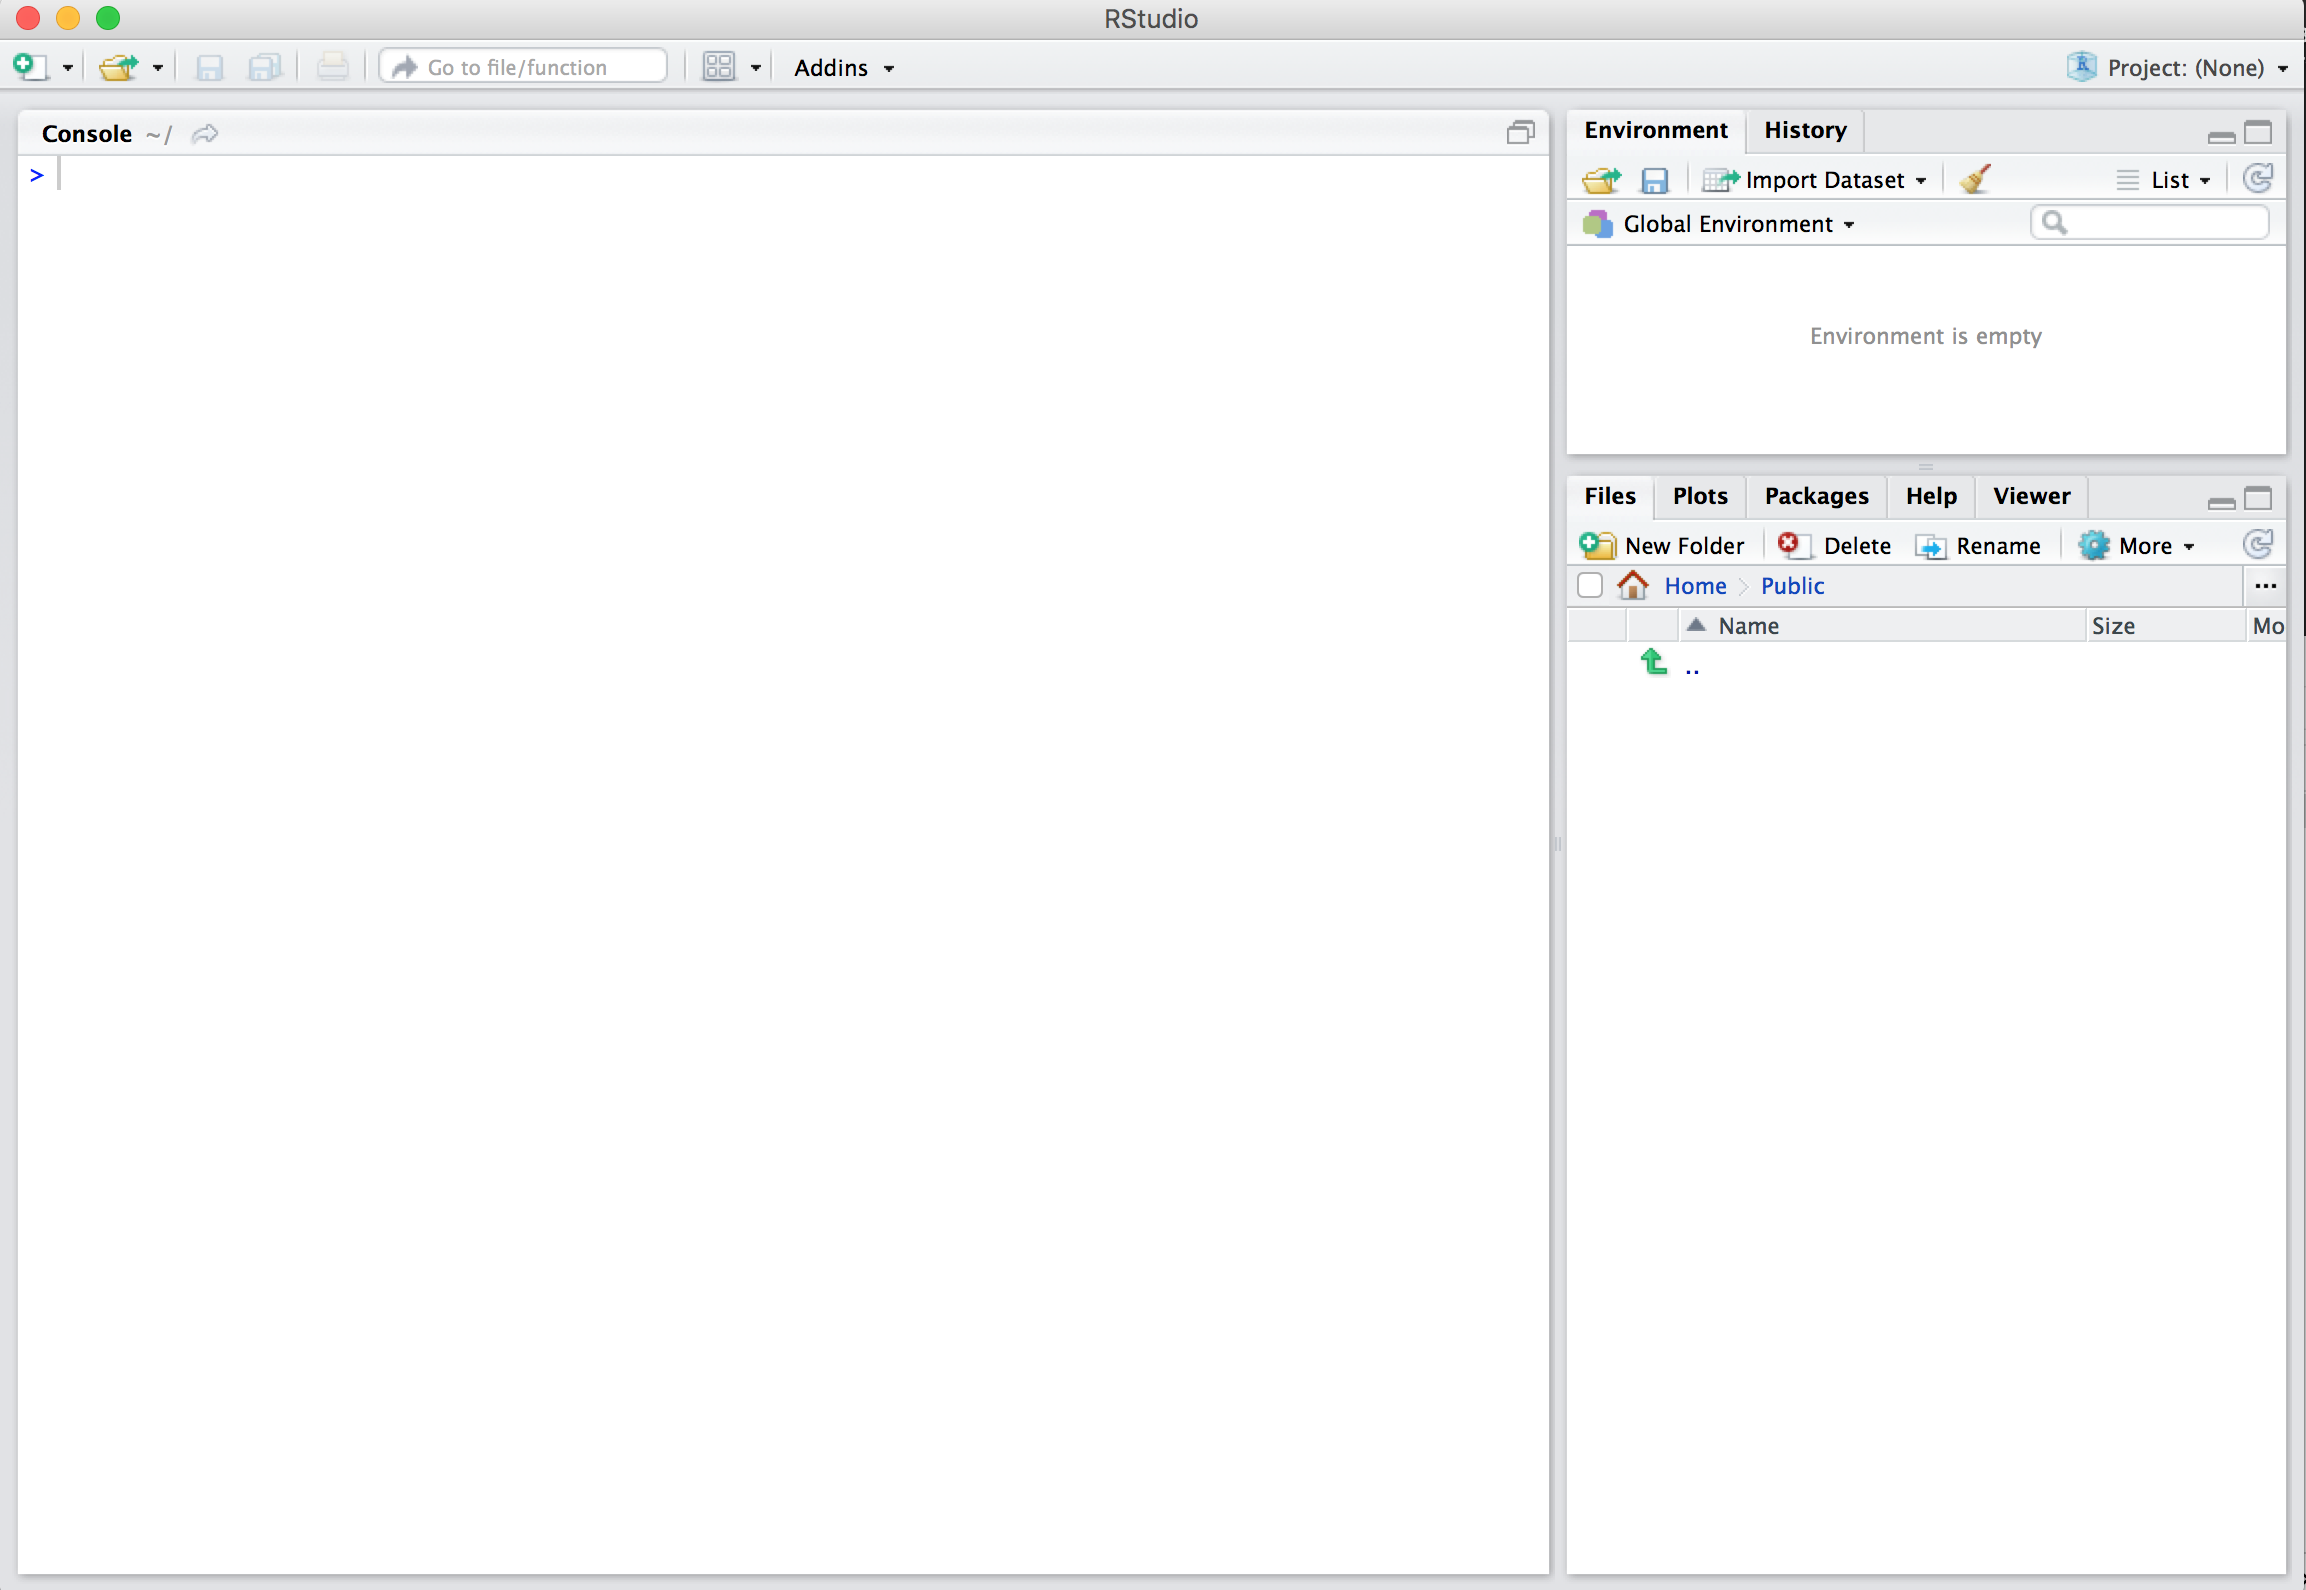
\includegraphics{images/rstudio.png}

Prenez le temps d'explorer cette interface, cliquez sur les différents
onglets, ouvrez les menus, allez faire un tour dans les préférences du
logiciel pour découvrir les différents panneaux de l'application, en
particulier la Console dans laquelle nous exécuterons très bientôt du
code \texttt{R}.

\section{\texorpdfstring{Comment exécuter du code \texttt{R}
?}{Comment exécuter du code R ?}}\label{sec-code}

Contrairement à d'autres logiciels comme Excel, STATA ou SAS qui
fournissent des interfaces où tout se fait en cliquant avec sa souris,
\texttt{R} est un langage interprété, ce qui signifie que vous devez
taper des commandes, écrites en code \texttt{R}. C'est-à-dire que vous
devez \textbf{programmer} en \texttt{R} (j'utilise les termes ``coder''
et ``programmer'' de manière interchangeable dans ce livre).

Il n'est pas nécessaire d'être un programmeur pour utiliser \texttt{R},
néanmoins, il est nécessaire de programmer ! Il existe en effet un
ensemble de concepts de programmation de base que les utilisateurs de
\texttt{R} doivent comprendre et maîtriser. Et progresser en
programmation vous permettra d'automatiser de plus en plus de choses, et
donc, à terme, de gagner beaucoup de temps. Par conséquent, bien que ce
livre ne soit pas un livre sur la programmation, vous en apprendrez
juste assez en programmation pour explorer et analyser efficacement des
données.

\subsection{La console}\label{la-console}

La façon la plus simple d'interagir avec \texttt{RStudio} (mais pas du
tout la meilleure !) consiste à taper directement des commandes que
\texttt{R} pourra comprendre \textbf{dans la Console}.

Cliquez dans la console (après le symbole \texttt{\textgreater{}}) et
tapez ceci, sans oublier de valider en tapant sur la touche
\texttt{Entrée} :

\begin{Shaded}
\begin{Highlighting}[]
\DecValTok{3} \SpecialCharTok{+} \DecValTok{8}
\end{Highlighting}
\end{Shaded}

\begin{verbatim}
[1] 11
\end{verbatim}

Félicitations, vous venez de taper votre première instruction \texttt{R}
: vous savez maintenant faire des additions !

Dans la version en ligne de ce livre (en html), à chaque fois que du
code \texttt{R} sera fourni, il apparaîtra dans un cadre grisé avec une
ligne bleue à gauche, comme ci-dessus. Vous pourrez toujours taper dans
\texttt{RStudio}, les commandes qui figurent dans ces blocs de code,
afin d'obtenir vous même les résultats souhaités. Dans ce livre, lorsque
les commandes \texttt{R} produisent des résultats, ils sont affichés
juste en dessous des blocs de code. Enfin, en passant la souris sur les
blocs de code, vous verrez apparaître, à droite, une icône de
presse-papier qui vous permettra de copier-coller les commandes du livre
dans la console de \texttt{RStudio} ou, très bientôt, dans vos scripts.

\begin{tcolorbox}[enhanced jigsaw, colbacktitle=quarto-callout-warning-color!10!white, colframe=quarto-callout-warning-color-frame, bottomtitle=1mm, opacityback=0, arc=.35mm, leftrule=.75mm, titlerule=0mm, colback=white, title=\textcolor{quarto-callout-warning-color}{\faExclamationTriangle}\hspace{0.5em}{Les risques du ``copier-coller'' {\faIcon{clipboard}}}, toptitle=1mm, breakable, coltitle=black, rightrule=.15mm, left=2mm, opacitybacktitle=0.6, toprule=.15mm, bottomrule=.15mm]

Attention : il est fortement conseillé de réserver les copier-coller aux
blocs de commandes de (très) grande taille, ou en cas d'erreur de
syntaxe inexplicable. L'expérience a en effet montré qu'\textbf{on
apprend beaucoup mieux {en tapant soi-même les commandes}}. Ça n'est que
comme cela que l'on peut prendre conscience de toutes les subtilités du
langage (par exemple, faut-il mettre une virgule ou un point, une
parenthèse ou un crochet, le symbole moins ou un tilde, etc.). Je vous
conseille donc de taper vous-même les commandes autant que possible.

\end{tcolorbox}

\subsection{Les scripts}\label{sec-script}

Taper du code directement dans la console est probablement la pire façon
de travailler dans \texttt{RStudio}. Cela est parfois utile pour faire
un rapide calcul, ou pour vérifier qu'une commande fonctionne
correctement. Mais la plupart du temps, \textbf{vous devriez taper vos
commandes dans un script}.

\begin{tcolorbox}[enhanced jigsaw, colbacktitle=quarto-callout-important-color!10!white, colframe=quarto-callout-important-color-frame, bottomtitle=1mm, opacityback=0, arc=.35mm, leftrule=.75mm, titlerule=0mm, colback=white, title=\textcolor{quarto-callout-important-color}{\faExclamation}\hspace{0.5em}{Définition importante !}, toptitle=1mm, breakable, coltitle=black, rightrule=.15mm, left=2mm, opacitybacktitle=0.6, toprule=.15mm, bottomrule=.15mm]

Un script est un fichier au format ``texte brut'' (cela signifie qu'il
n'y a pas de mise en forme et que ce fichier peut-être ouvert par
n'importe quel éditeur de texte, y compris les plus simples comme le
bloc notes de Windows), dans lequel vous pouvez taper :

\begin{enumerate}
\def\labelenumi{\arabic{enumi}.}
\tightlist
\item
  des instructions qui seront comprises par \texttt{R} comme si vous les
  tapiez directement dans la console
\item
  des lignes de commentaires, qui doivent obligatoirement commencer par
  le symbole \texttt{\#}.
\end{enumerate}

\end{tcolorbox}

Les avantages de travailler dans un script sont nombreux :

\begin{enumerate}
\def\labelenumi{\arabic{enumi}.}
\tightlist
\item
  Vous pouvez sauvegarder votre script à tout moment (vous devriez
  prendre l'habitude de le sauvegarder très régulièrement). Vous gardez
  ainsi la trace de toutes les commandes que vous avez tapées.
\item
  Vous pouvez aisément partager votre script pour collaborer avec vos
  collègues de promo et enseignants.
\item
  Vous pouvez documenter votre démarche et les différentes étapes de vos
  analyses. \textbf{Vous devez ajouter autant de commentaires que
  possible}. Cela permettra à vos collaborateurs de comprendre ce que
  vous avez fait. Et dans 6 mois, cela vous permettra de comprendre ce
  que vous avez fait. Si votre démarche vous paraît cohérente
  aujourd'hui, il n'est en effet pas garanti que vous vous souviendrez
  de chaque détail quand vous vous re-plongerez dans vos analyses dans
  quelques temps. Donc aidez-vous vous même en commentant vos scripts
  dès maintenant.
\item
  Un script bien structuré, bien indenté (avec les bons retours à la
  ligne, des sauts de lignes, des espaces, bref, de l'air) et clair
  permet de rendre vos analyses répétables. Si vous passez 15 heures à
  analyser un tableau de données précis, il vous suffira de quelques
  secondes pour analyser un nouveau jeu de données similaire : vous
  n'aurez que quelques lignes à modifier dans votre script original pour
  l'appliquer à de nouvelles données.
\end{enumerate}

Vous pouvez créer un script en cliquant dans le menu ``File
\textgreater{} New File \textgreater{} R Script''. Un nouveau panneau
s'ouvre dans l'application. Pensez à sauvegarder immédiatement votre
nouveau script en cliquant dans le menu ``File \textgreater{} Save'' ou
``File \textgreater{} Save as\ldots{}''. Il faut pour cela lui donner un
nom et choisir un emplacement sur votre disque dur.

\begin{tcolorbox}[enhanced jigsaw, colbacktitle=quarto-callout-important-color!10!white, colframe=quarto-callout-important-color-frame, bottomtitle=1mm, opacityback=0, arc=.35mm, leftrule=.75mm, titlerule=0mm, colback=white, title=\textcolor{quarto-callout-important-color}{\faExclamation}\hspace{0.5em}{Où sauvegarder vos scripts ? {\faIcon{save}}}, toptitle=1mm, breakable, coltitle=black, rightrule=.15mm, left=2mm, opacitybacktitle=0.6, toprule=.15mm, bottomrule=.15mm]

Je vous encourage vivement à créer, sur votre disque dur, un nouveau
dossier spécifique, que vous nommerez par exemple
\texttt{Data\_Analysis}. Il est important que le nom de ce dossier ne
contienne pas de caractères spéciaux (\emph{e.g.} accents, cédilles,
apostrophes, espaces, etc.). Ce dossier devrait être facilement
accessible : vous y enregistrerez tous vos scripts, vos jeux de données,
vos graphiques, etc.

Si vous travaillez sur les ordinateurs de l'université, créez
{obligatoirement} votre dossier sur le disque
\texttt{W:\textbackslash{}}. Il s'agit de votre espace personnel sur le
réseau de l'université. Cela vous garantit que vous retrouverez votre
script la prochaine fois, même si vous utilisez un ordinateur différent.

\end{tcolorbox}

À partir de maintenant, vous ne devriez plus taper de commande
directement dans la console. Tapez systématiquement vos commandes dans
un script et sauvegardez-le régulièrement.

Pour exécuter les commandes du script dans la console, il suffit de
placer le curseur sur la ligne contenant la commande et de presser les
touches \texttt{ctrl\ +\ enter} (ou \texttt{command\ +\ enter} sous
macOS). Si un message d'erreur s'affiche dans la console, c'est que
votre instruction était erronée. Modifiez la directement dans votre
script et pressez à nouveau les touches \texttt{ctrl\ +\ enter} (ou
\texttt{command\ +\ enter} sous macOS) pour tenter à nouveau votre
chance. Idéalement, votre script ne devrait contenir que des commandes
qui fonctionnent et des commentaires expliquant à quoi servent ces
commandes.

Voici un exemple de script que je ne vous demande pas de reproduire.
Lisez simplement attentivement son contenu :

\begin{Shaded}
\begin{Highlighting}[]
\CommentTok{\# Penser à installer le package ggplot2 si besoin}
\CommentTok{\# install.packages("ggplot2")}

\CommentTok{\# Chargement du package}
\FunctionTok{library}\NormalTok{(ggplot2)}

\CommentTok{\# Mise en mémoire des données de qualité de l\textquotesingle{}air à New{-}York de mai à}
\CommentTok{\# septembre 1973}
\FunctionTok{data}\NormalTok{(airquality)}

\CommentTok{\# Affichage des premières lignes du tableau de données}
\FunctionTok{head}\NormalTok{(airquality)}

\CommentTok{\# Quelle est la structure de ce tableau ?}
\FunctionTok{str}\NormalTok{(airquality)}

\CommentTok{\# Réalisation d\textquotesingle{}un graphique présentant la relation entre la concentration}
\CommentTok{\# en ozone atmosphérique en ppb et la température en degrés Fahrenheit}
\FunctionTok{ggplot}\NormalTok{(}\AttributeTok{data =}\NormalTok{ airquality, }\AttributeTok{mapping =} \FunctionTok{aes}\NormalTok{(}\AttributeTok{x =}\NormalTok{ Temp, }\AttributeTok{y =}\NormalTok{ Ozone)) }\SpecialCharTok{+}
  \FunctionTok{geom\_point}\NormalTok{() }\SpecialCharTok{+}
  \FunctionTok{geom\_smooth}\NormalTok{(}\AttributeTok{method =} \StringTok{"loess"}\NormalTok{)}

\CommentTok{\# On constate une augmentation importante de la concentration d\textquotesingle{}ozone }
\CommentTok{\# pour des températures supérieures à 75ºF}
\end{Highlighting}
\end{Shaded}

Même si vous ne comprenez pas encore les commandes qui figurent dans ce
script (ça viendra !), voici ce que vous devez en retenir :

\begin{enumerate}
\def\labelenumi{\arabic{enumi}.}
\tightlist
\item
  Le script contient plus de lignes de commentaires que de commandes
  \texttt{R}.
\item
  Chaque étape de l'analyse est décrite en détail.
\item
  Les 2 dernières lignes du script décrivent les résultats obtenus (ici,
  un graphique).
\item
  Seules des commandes pertinentes et qui fonctionnent ont été
  conservées dans ce script.
\item
  Chaque ligne de commentaire commence par \texttt{\#}. Il est ainsi
  possible de conserver certaines commandes \texttt{R} dans le script,
  ``pour mémoire'', sans pour autant qu'elle ne soient exécutées. C'est
  le cas pour la ligne \texttt{\#\ install.packages("ggplot2")}.
\end{enumerate}

Si j'exécute ce script dans la console de \texttt{RStudio} (en
sélectionnant toutes les lignes et en pressant les touches
\texttt{ctrl\ +\ enter} ou \texttt{command\ +\ enter} sous macOS), voilà
ce qui est produit :

\begin{verbatim}
  Ozone Solar.R Wind Temp Month Day
1    41     190  7.4   67     5   1
2    36     118  8.0   72     5   2
3    12     149 12.6   74     5   3
4    18     313 11.5   62     5   4
5    NA      NA 14.3   56     5   5
6    28      NA 14.9   66     5   6
\end{verbatim}

\begin{verbatim}
'data.frame':   153 obs. of  6 variables:
 $ Ozone  : int  41 36 12 18 NA 28 23 19 8 NA ...
 $ Solar.R: int  190 118 149 313 NA NA 299 99 19 194 ...
 $ Wind   : num  7.4 8 12.6 11.5 14.3 14.9 8.6 13.8 20.1 8.6 ...
 $ Temp   : int  67 72 74 62 56 66 65 59 61 69 ...
 $ Month  : int  5 5 5 5 5 5 5 5 5 5 ...
 $ Day    : int  1 2 3 4 5 6 7 8 9 10 ...
\end{verbatim}

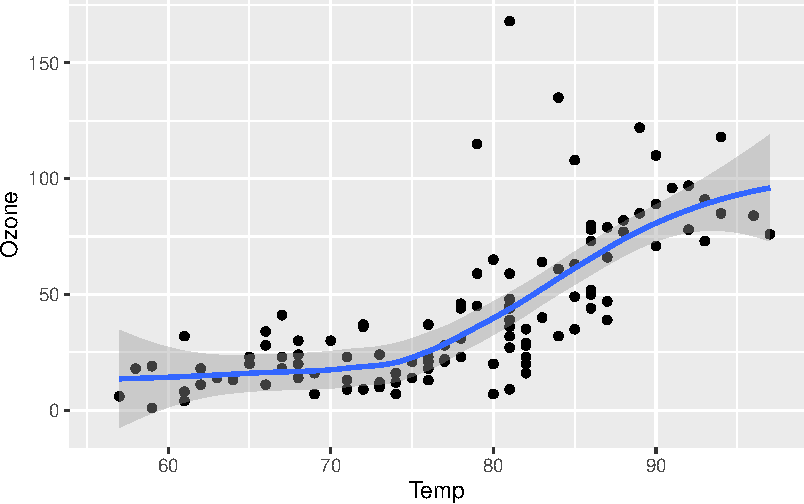
\includegraphics{01-RBasics_files/figure-pdf/unnamed-chunk-3-1.pdf}

\subsection{\texorpdfstring{Les projets, ou
\texttt{Rprojects}}{Les projets, ou Rprojects}}\label{sec-rproj}

Pour travailler le plus efficacement possible avec \texttt{RStudio},
vous devriez créer, à l'intérieur de votre dossier de travail, un
nouveau fichier très particulier, qui s'appelle, dans le jargon de
\texttt{RStudio}, un \textbf{\texttt{Rproject}}.

Pour le créer, cliquez simplement dans le Menu ``File \textgreater{} New
Project\ldots{}''. Cette boîte de dialogue devrait apparaître :

\begin{center}
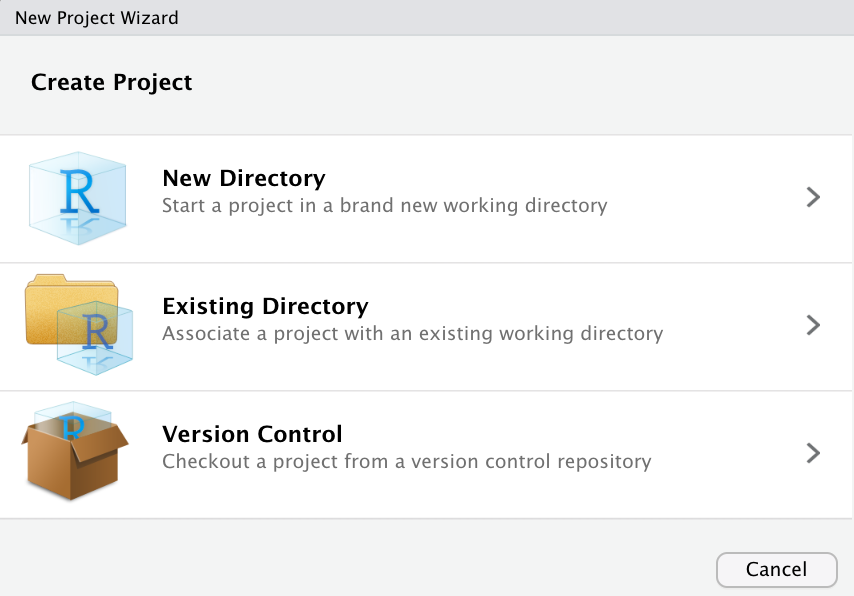
\includegraphics[width=0.6\textwidth,height=\textheight]{images/Rproj1.png}
\end{center}

Choisissez ``Existing Directory'', puis, dans la boîte de dialogue
suivante :

\begin{center}
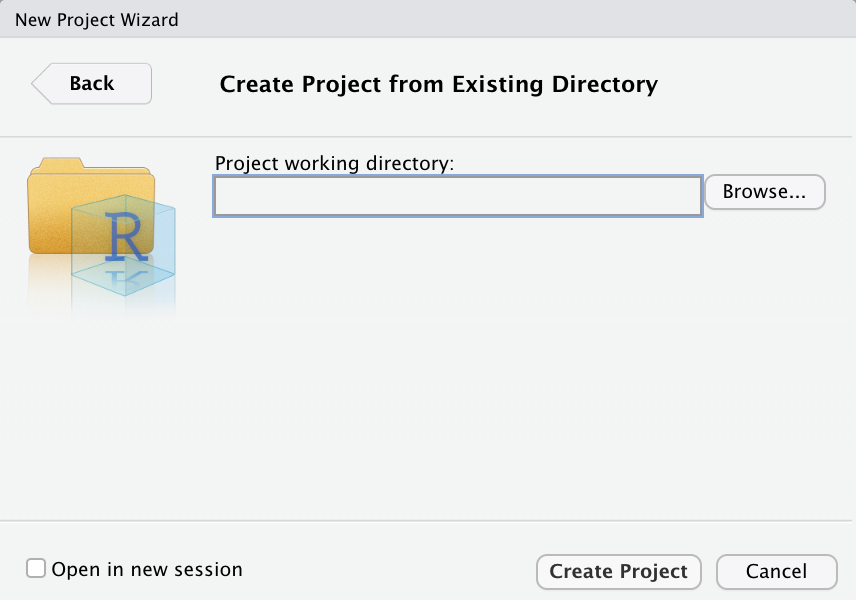
\includegraphics[width=0.6\textwidth,height=\textheight]{images/Rproj2.png}
\end{center}

cliquez sur ``Browse\ldots{}'', naviguez jusqu'au dossier que vous avez
créé plus tôt sur votre disque dur et qui contient votre script, puis
cliquez sur ``Create Project''. La fenêtre de \texttt{RStudio} se ferme,
puis une nouvelle fenêtre vierge apparaît. En apparence, rien n'a changé
ou presque. Pourtant :

\begin{enumerate}
\def\labelenumi{\arabic{enumi}.}
\tightlist
\item
  en haut à droite de la fenêtre de \texttt{RStudio}, le logiciel
  indique maintenant que vous êtes bel et bien à l'intérieur d'un
  \texttt{Rproject}. Au lieu de \texttt{Project:\ (None)}, on lit
  maintenant le nom du \texttt{Rproject} (chez moi,
  \texttt{Data\_Analysis})
\item
  dans le quart inférieur droit de l'interface, l'onglet ``Files'' ne
  présente plus le même aspect. Avant de créer le \texttt{Rproject}, cet
  onglet présentait le chemin vers le dossier utilisé par défaut par le
  logiciel, ainsi que son contenu. Il s'agissait d'un dossier système
  auquel il vaut mieux ne pas toucher pour éviter les problèmes. Après
  la création du \texttt{Rproject}, l'onglet ``Files'' indique le
  contenu du dossier contenant le projet. Autrement dit, c'est ici que
  vous trouverez vos scripts, tableaux de données dans différents
  formats, figures sauvegardées, etc. Dans cet onglet, vous pouvez donc
  cliquer sur le nom de votre script pour l'ouvrir à nouveau, le
  modifier, l'exécuter\ldots{}
\end{enumerate}

\begin{figure}

\begin{minipage}{0.50\linewidth}

\begin{figure}[H]

{\centering 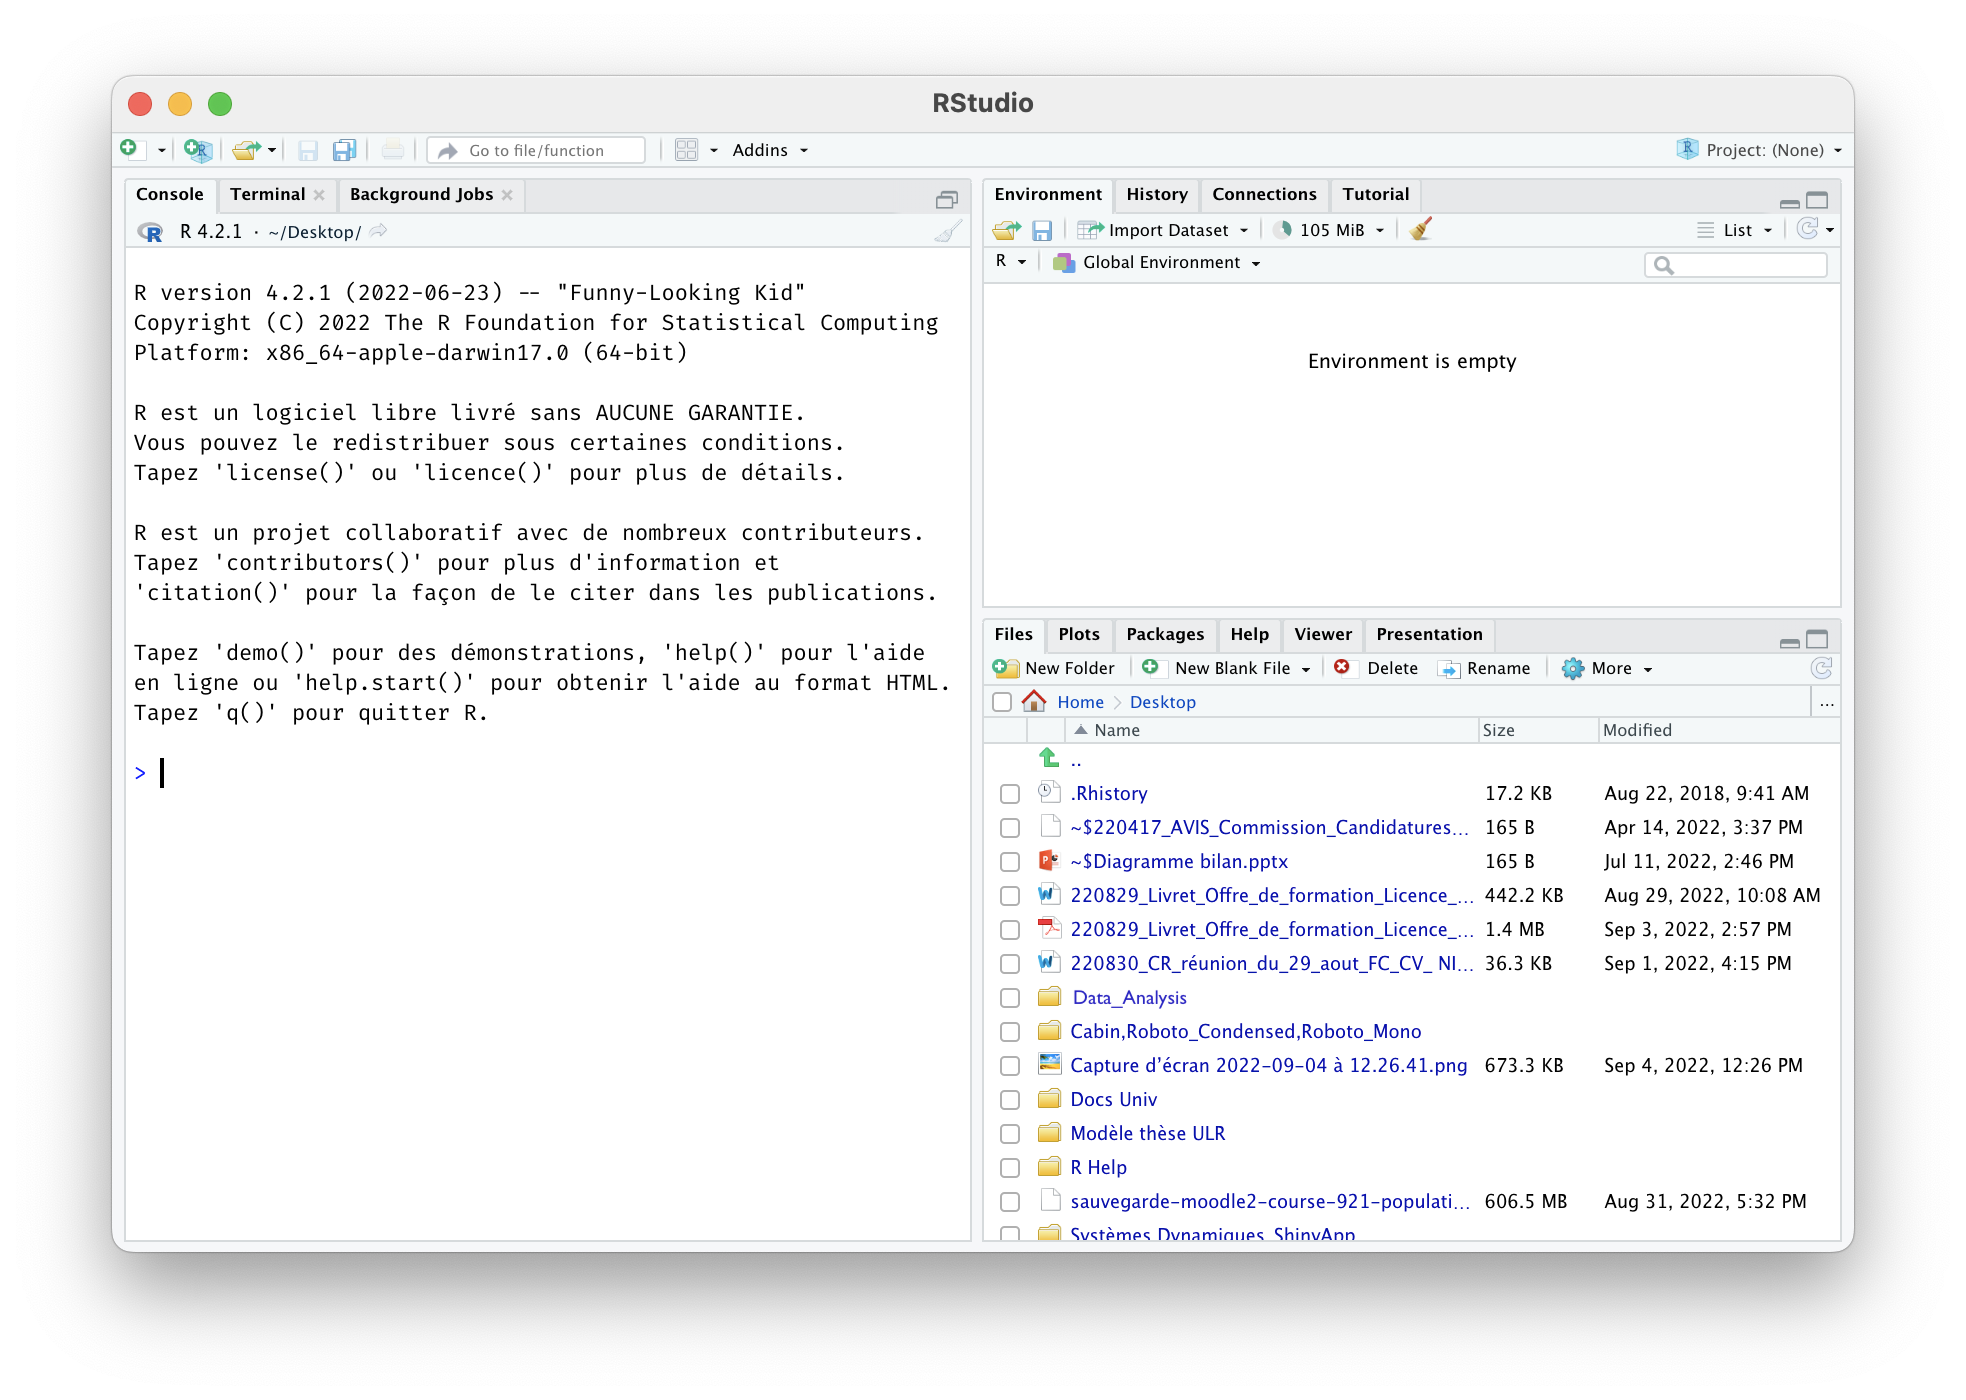
\includegraphics{images/Avant.png}

}

\subcaption{Sans \texttt{Rproject}}

\end{figure}%

\end{minipage}%
%
\begin{minipage}{0.50\linewidth}

\begin{figure}[H]

{\centering 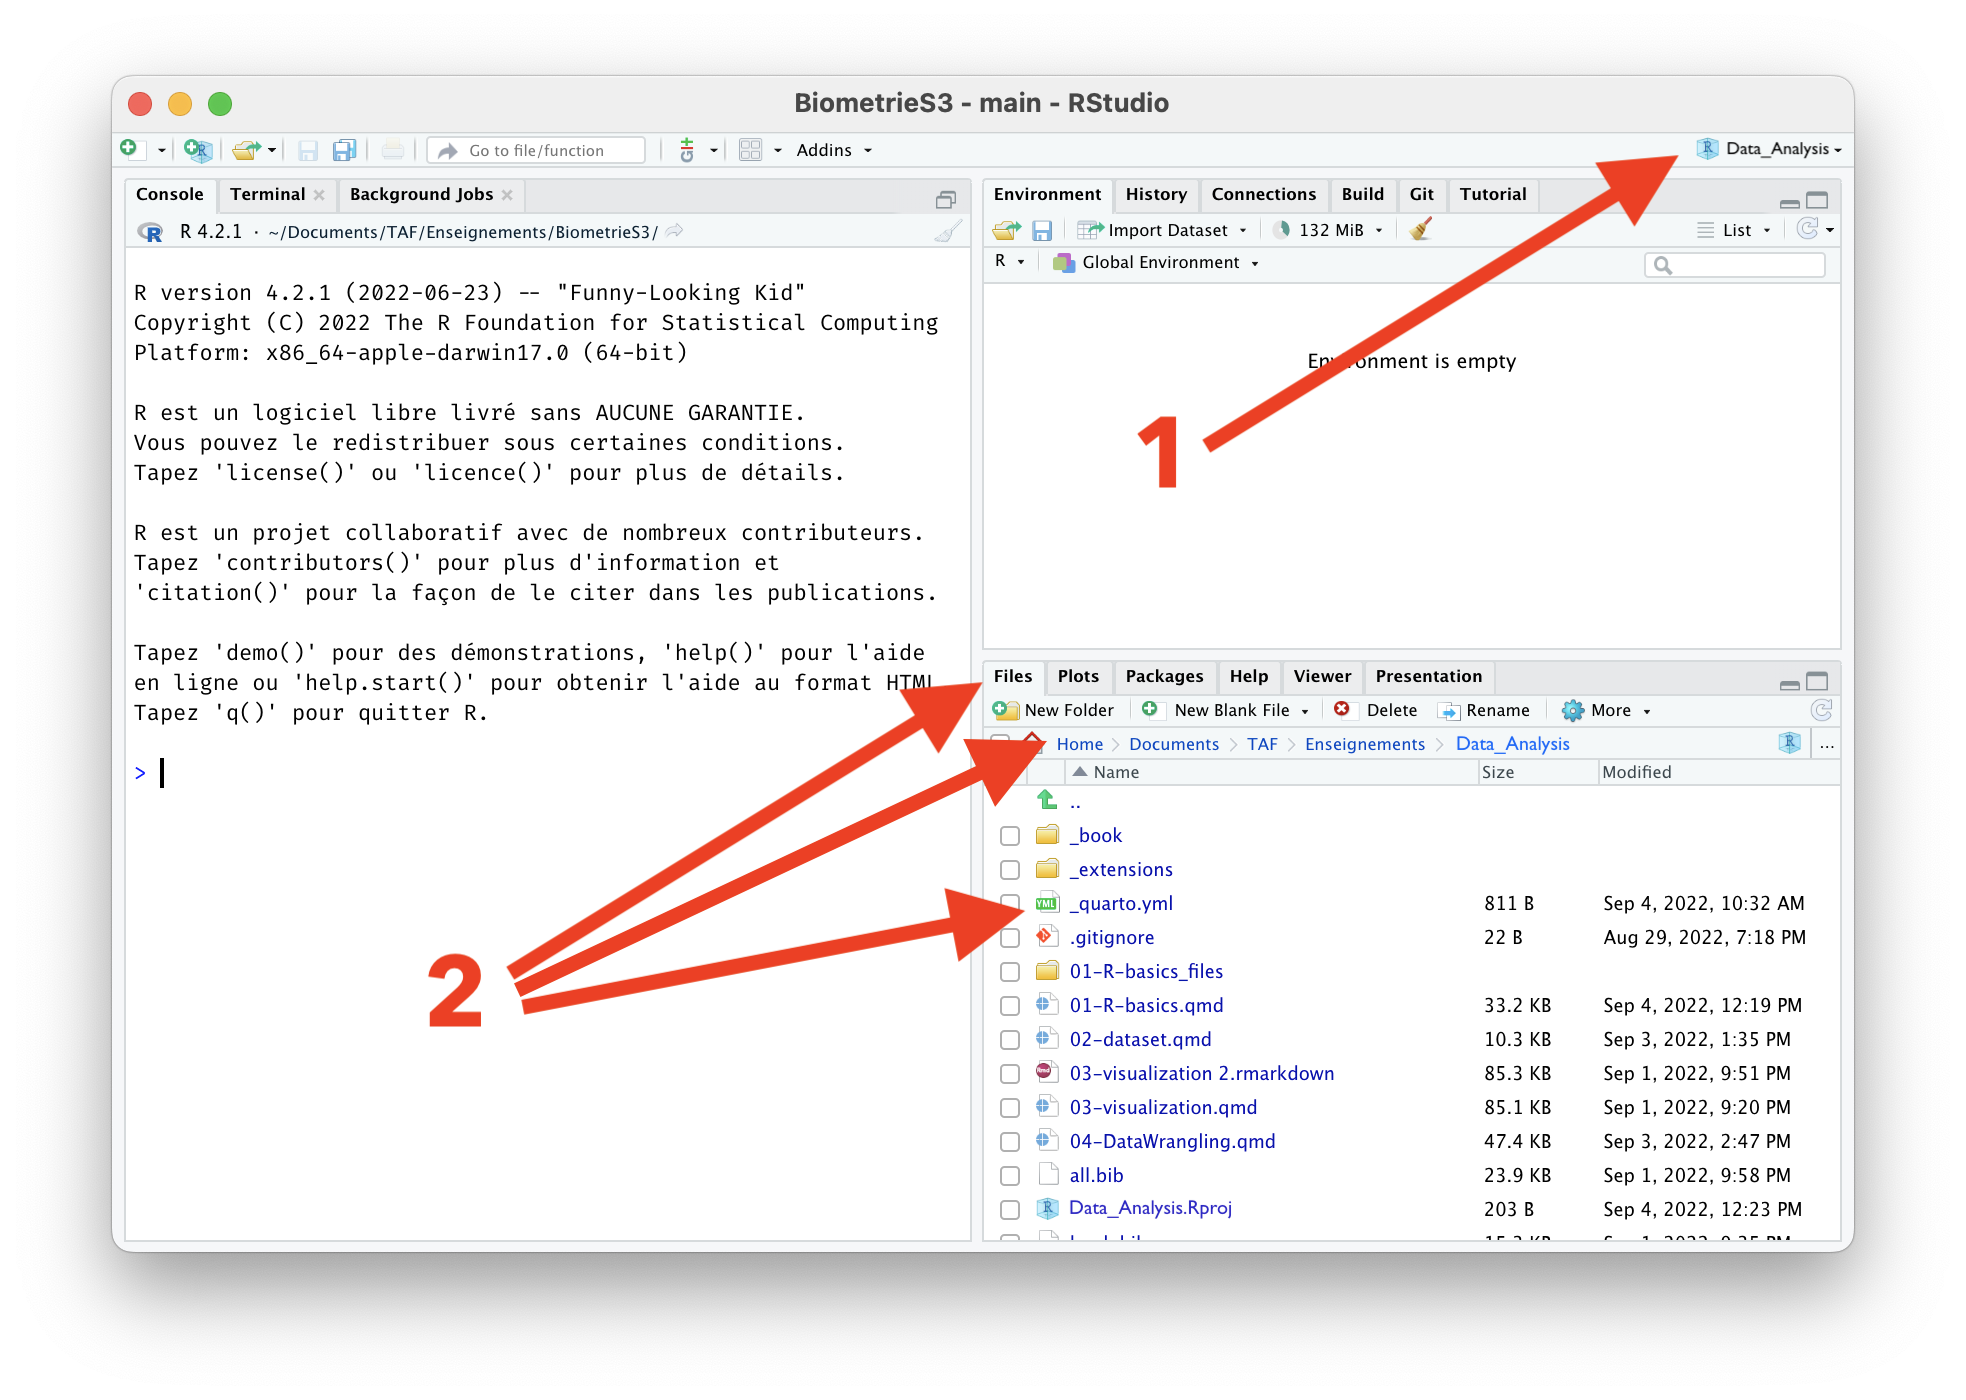
\includegraphics{images/Après.png}

}

\subcaption{Avec \texttt{RProject}}

\end{figure}%

\end{minipage}%

\end{figure}%

\begin{enumerate}
\def\labelenumi{\arabic{enumi}.}
\setcounter{enumi}{2}
\tightlist
\item
  un nouveau fichier portant l'extension \texttt{.Rproj} a été créé dans
  votre dossier de travail. La prochaine fois que vous voudrez
  travailler dans \texttt{RStudio}, il vous suffira de double-cliquer
  sur ce fichier dans l'explorateur de fichier de Windows ou le Finder
  de MacOS, pour que \texttt{RStudio} s'ouvre, et que vous retrouviez
  tous vos fichiers et scripts de la fois précédente
\end{enumerate}

\begin{center}

\includegraphics[width=0.2\textwidth,height=\textheight]{images/Rproj3.png}
\end{center}

Pour vérifier que tout s'est bien passé jusqu'ici, tapez la commande
suivante dans votre script puis envoyez-la dans la console en pressant
les touches \texttt{ctrl\ +\ entrée} (ou \texttt{command\ +\ entrée}
sous MacOS).

\begin{Shaded}
\begin{Highlighting}[]
\FunctionTok{getwd}\NormalTok{()}
\end{Highlighting}
\end{Shaded}

\texttt{RStudio} doit vous afficher, dans la console, le chemin jusqu'à
votre {répertoire de travail} ou ``Working Directory'' en anglais
(\texttt{getwd()} est l'abréviation de ``GET Working Directory''). Si
tout s'est bien passé, ce chemin doit être celui du dossier qui contient
votre script et le fichier \texttt{.Rproj} que vous venez de créer. Si
ce n'est pas le cas, reprenez calmement toutes les étapes décrites
depuis le début de la Section~\ref{sec-script}. Si ça ne fonctionne
toujours pas, contactez-moi sur Slack.

\begin{tcolorbox}[enhanced jigsaw, colbacktitle=quarto-callout-important-color!10!white, colframe=quarto-callout-important-color-frame, bottomtitle=1mm, opacityback=0, arc=.35mm, leftrule=.75mm, titlerule=0mm, colback=white, title=\textcolor{quarto-callout-important-color}{\faExclamation}\hspace{0.5em}{Pour résumer\ldots{} \faIcon{laptop-code}}, toptitle=1mm, breakable, coltitle=black, rightrule=.15mm, left=2mm, opacitybacktitle=0.6, toprule=.15mm, bottomrule=.15mm]

Les \texttt{Rprojects} sont un moyen très pratique de travailler
efficacement dans \texttt{RStudio} car ils permettent de gérer
facilement la question du répertoire de travail. Lorsque vous envisagez
de travailler sur un nouveau sujet/projet/jeu de données/compte-rendu de
TP\ldots, les étapes à suivre, pour vous mettre dans une configuration
idéale qui vous évitera bien des problèmes par la suite, sont donc les
suivantes :

\begin{enumerate}
\def\labelenumi{\arabic{enumi}.}
\tightlist
\item
  Sur votre ordinateur, créez un nouveau dossier avec un nom simple, et
  à un endroit facile d'accès (pas de caractères spéciaux dans le chemin
  du dossier si possible)
\item
  Démarrez \texttt{RStudio}
\item
  Dans le logiciel, cliquez dans le menu ``File \textgreater{} New
  Project\ldots{}''
\item
  Choisissez ``Existing Directory'', puis naviguez jusqu'au dossier que
  vous venez de créer
\item
  Cliquez sur ``Create Project''
\item
  Créer un nouveau script (menu ``File \textgreater{} New File
  \textgreater{} R script'')
\item
  Donnez un nom à votre script (menu ``File \textgreater{} Save
  As\ldots{}'') pour le sauvegarder. Par défaut, \texttt{RStudio} vous
  propose d'enregistrer votre script dans le dossier de votre
  \texttt{Rproject}, ce qui est parfait.
\item
  Tapez \texttt{getwd()} dans votre script et exécutez cette commande en
  l'envoyant dans la console.
\end{enumerate}

Si le chemin qui s'affiche est celui du dossier contenant votre
\texttt{Rproject} et votre script, félicitation, vous êtes prêt·e à
travailler. Avec un peu d'habitude, ces étapes ne prennent qu'une à deux
minutes.

\end{tcolorbox}

\subsection{Concepts de base en programmation et
terminologie}\label{concepts-de-base-en-programmation-et-terminologie}

Après ces considérations techniques sur l'utilisation et les réglages de
\texttt{RStudio}, nous entrons maintenant dans le vif du sujet avec la
découverte des premiers éléments de syntaxe du langage \texttt{R}.

\subsubsection{Objets, types, vecteurs, facteurs et tableaux de
données}\label{sec-objects}

Pour vous présenter les concepts de base et la terminologie de la
programmation dont nous aurons besoin, vous allez suivre des tutoriels
en ligne sur le site de DataCamp. Pour cette première prise en main,
tout va maintenant se passer dans votre navigateur internet, et vous
pouvez donc mettre de côté \texttt{RStudio} pour l'instant. Vous allez
voir que l'interface de DataCamp ressemble à une version simplifiée de
l'éditeur de script et de la console de \texttt{RStudio} : vous n'aurez
pas à vous soucier des réglages, de \texttt{Rprojects} ou de sauvegarder
quoi que ce soit. Si vous avez correctement créé votre compte gratuit
DataCamp comme indiqué au tout début de la Chapitre~\ref{sec-basics},
votre progression sera sauvegardée automatiquement. Il vous suffit de
cliquer sur les liens direct ci-dessous pour démarrer les tutoriels en
ligne.

Avant de démarrer, quelques précisions :

\begin{itemize}
\tightlist
\item
  pour chaque tutoriel que je vous demande de suivre, j'indique
  ci-dessous une liste des concepts de programmation qui sont couverts.
  N'hésitez pas à vous y référer et à y revenir tout au long du master
  (et au-delà !) si vous avez oublié certaines choses
\item
  ce tutoriel DataCamp contient 6 chapitres. Seuls les chapitres 1, 2,
  4, et 5 doivent être suivis. Nous ne travaillerons pas sur les
  matrices ni sur les listes
\item
  à la fin de chaque chapitre du tutoriel, revenez à ce livre en ligne
  pour cliquer sur le lien direct ver le chapitre suivant. Procéder
  ainsi vous évitera de suivre des chapitres inutiles du tutoriel, et
  cela vous permettra également d'éviter les demandes d'inscriptions
  payantes à DataCamp
\end{itemize}

Il est important de noter que, bien que ces tutoriels sont d'excellentes
introductions, une lecture seule, même attentive, est insuffisante pour
un apprentissage en profondeur et une rétention à long terme. Il faut
pour cela \textbf{pratiquer} et \textbf{répéter}. Outre les exercices
demandés dans DataCamp, que vous devez effectuer directement dans votre
navigateur, je vous encourage à prendre des notes, à multiplier les
essais, directement dans la console de \texttt{RStudio}, ou, de
préférence, dans un script que vous annoterez, pour vous assurer que
vous avez bien compris chaque partie.

Allez maintenant découvrir
\href{https://app.datacamp.com/learn/courses/introduction-a-r}{le cours
d'introduction à R} sur DataCamp, et cliquez sur les liens des chapitres
ci-dessous. Au fur et à mesure de votre travail, notez les termes
importants et ce à quoi ils font référence.

\begin{itemize}
\tightlist
\item
  \href{https://campus.datacamp.com/courses/introduction-a-r/chapitre-1-introduction?ex=1}{Chapitre
  1 : introduction}

  \begin{itemize}
  \tightlist
  \item
    La console : l'endroit où vous tapez des commandes
  \item
    Les objets : où les valeurs sont stockées, comment assigner des
    valeurs à des objets
  \item
    Les types de données : entiers, doubles/numériques, caractères et
    logiques
  \end{itemize}
\item
  \href{https://campus.datacamp.com/courses/introduction-a-r/chapitre-2-les-vecteurs?ex=1}{Chapitre
  2 : vecteurs}

  \begin{itemize}
  \tightlist
  \item
    Les vecteurs : des collections de valeurs du même type
  \end{itemize}
\item
  \href{https://campus.datacamp.com/courses/introduction-a-r/chapitre-4-facteurs?ex=1}{Chapitre
  4 : les facteurs}

  \begin{itemize}
  \tightlist
  \item
    Des données catégorielles (et non pas \emph{numériques})
    représentées dans \texttt{R} sous forme de \texttt{factor}s
  \end{itemize}
\item
  \href{https://campus.datacamp.com/courses/introduction-a-r/chapitre-5-les-jeux-de-donnees?ex=1}{Chapitre
  5 : les jeux de données ou \texttt{data.frame}}

  \begin{itemize}
  \tightlist
  \item
    Les \texttt{data.frame}s sont similaires aux feuilles de calcul
    rectangulaires que l'on peut produire dans un tableur. Dans
    \texttt{R}, ce sont des objets rectangulaires (des tableaux !)
    contenant des jeux de données : les lignes correspondent aux
    observations et les colonnes aux variables décrivant les
    observations. La plupart du temps, c'est le format de données que
    nous utiliserons. Plus de détails dans le Chapitre~\ref{sec-dataset}
  \end{itemize}
\end{itemize}

Avant de passer à la suite, il nous reste 2 grandes notions à découvrir
dans le domaine du code et de la syntaxe afin de pouvoir travailler
efficacement dans \texttt{R} : les opérateurs de comparaison d'une part,
et les fonctions d'autre part. Pour les découvrir et expérimenter, et
puisque vous avez terminé les tutoriels DataCamp, reprenez maintenant
\texttt{RStudio} et travaillez dans votre script.

\subsubsection{Opérateurs de comparaison}\label{sec-comparaison}

Comme leur nom l'indique, ils permettent de comparer des valeurs ou des
objets. Les principaux opérateurs de comparaison sont :

\begin{itemize}
\tightlist
\item
  \texttt{==} : égal à
\item
  \texttt{!=} : différent de
\item
  \texttt{\textgreater{}} : supérieur à
\item
  \texttt{\textless{}} : inférieur à
\item
  \texttt{\textgreater{}=} : supérieur ou égal à
\item
  \texttt{\textless{}=} : inférieur ou égal à
\end{itemize}

Ainsi, on peut tester si 3 est égal à 5 :

\begin{Shaded}
\begin{Highlighting}[]
\DecValTok{3} \SpecialCharTok{==} \DecValTok{5}
\end{Highlighting}
\end{Shaded}

\begin{verbatim}
[1] FALSE
\end{verbatim}

La réponse est bien entendu \texttt{FALSE}. Est-ce que 3 est inférieur à
5 ?

\begin{Shaded}
\begin{Highlighting}[]
\DecValTok{3} \SpecialCharTok{\textless{}} \DecValTok{5}
\end{Highlighting}
\end{Shaded}

\begin{verbatim}
[1] TRUE
\end{verbatim}

La réponse est maintenant \texttt{TRUE}. Lorsque l'on utilise un
opérateur de comparaison, la réponse est toujours soit vrai
(\texttt{TRUE}), soit faux (\texttt{FALSE}).

Il est aussi possible de comparer des chaînes de charactères :

\begin{Shaded}
\begin{Highlighting}[]
\StringTok{"Bonjour"} \SpecialCharTok{==} \StringTok{"Au revoir"}
\end{Highlighting}
\end{Shaded}

\begin{verbatim}
[1] FALSE
\end{verbatim}

\begin{Shaded}
\begin{Highlighting}[]
\StringTok{"Bonjour"} \SpecialCharTok{\textgreater{}=} \StringTok{"Au revoir"}
\end{Highlighting}
\end{Shaded}

\begin{verbatim}
[1] TRUE
\end{verbatim}

Manifestement, ``Bonjour'' est supérieur ou égal à ``Au revoir''. En
fait, \texttt{R} utilise l'ordre alphabétique pour comparer les chaînes
de caractères. Puisque dans l'alphabet, le ``B'' de ``Bonjour'' arrive
après le ``A'' de ``Au revoir'', pour \texttt{R}, ``Bonjour'' est
supérieur à ``Au revoir''.

Il est également possible d'utiliser ces opérateurs pour comparer un
chiffre et un vecteur :

\begin{Shaded}
\begin{Highlighting}[]
\NormalTok{tailles\_pop1 }\OtherTok{\textless{}{-}} \FunctionTok{c}\NormalTok{(}\DecValTok{112}\NormalTok{, }\DecValTok{28}\NormalTok{, }\DecValTok{86}\NormalTok{, }\DecValTok{14}\NormalTok{, }\DecValTok{154}\NormalTok{, }\DecValTok{73}\NormalTok{, }\DecValTok{63}\NormalTok{, }\DecValTok{48}\NormalTok{)}
\NormalTok{tailles\_pop1 }\SpecialCharTok{\textgreater{}} \DecValTok{80}
\end{Highlighting}
\end{Shaded}

\begin{verbatim}
[1]  TRUE FALSE  TRUE FALSE  TRUE FALSE FALSE FALSE
\end{verbatim}

Ici, l'opérateur nous permet d'identifier quels éléments du vecteur
\texttt{taille\_pop1} sont supérieurs à 80. Il s'agit des éléments
placés en première, troisième et cinquième positions.

Il est aussi possible de comparer 2 vecteurs qui contiennent le même
nombre d'éléments :

\begin{Shaded}
\begin{Highlighting}[]
\NormalTok{tailles\_pop2 }\OtherTok{\textless{}{-}} \FunctionTok{c}\NormalTok{(}\DecValTok{114}\NormalTok{, }\DecValTok{27}\NormalTok{, }\DecValTok{38}\NormalTok{, }\DecValTok{91}\NormalTok{, }\DecValTok{54}\NormalTok{, }\DecValTok{83}\NormalTok{, }\DecValTok{33}\NormalTok{, }\DecValTok{68}\NormalTok{)}
\NormalTok{tailles\_pop1 }\SpecialCharTok{\textgreater{}}\NormalTok{ tailles\_pop2}
\end{Highlighting}
\end{Shaded}

\begin{verbatim}
[1] FALSE  TRUE  TRUE FALSE  TRUE FALSE  TRUE FALSE
\end{verbatim}

Les comparaisons sont ici faites élément par élément. Ainsi, les
observations 2, 3, 5 et 7 du vecteur \texttt{tailles\_pop1} sont
supérieures aux observations 2, 3, 5 et 7 du vecteur
\texttt{tailles\_pop2} respectivement.

Ces vecteurs de vrais/faux sont très utiles car ils peuvent permettre de
compter le nombre d'éléments répondant à une certains condition :

\begin{Shaded}
\begin{Highlighting}[]
\FunctionTok{sum}\NormalTok{(tailles\_pop1 }\SpecialCharTok{\textgreater{}}\NormalTok{ tailles\_pop2)}
\end{Highlighting}
\end{Shaded}

\begin{verbatim}
[1] 4
\end{verbatim}

Lorsque l'on effectue une opération arithmétique (comme le calcul d'une
somme ou d'une moyenne) sur un vecteur de vrais/faux, les \texttt{TRUE}
sont remplacés par \texttt{1} et les \texttt{FALSE} par \texttt{0}. La
somme nous indique donc le nombre de vrais dans un vecteur de
vrais/faux, et la moyenne nous indique la proportion de vrais :

\begin{Shaded}
\begin{Highlighting}[]
\FunctionTok{mean}\NormalTok{(tailles\_pop1 }\SpecialCharTok{\textgreater{}}\NormalTok{ tailles\_pop2)}
\end{Highlighting}
\end{Shaded}

\begin{verbatim}
[1] 0.5
\end{verbatim}

\textbf{Note} : Attention, si les vecteurs comparés n'ont pas la même
taille, un message d'avertissement est affiché :

\begin{Shaded}
\begin{Highlighting}[]
\NormalTok{tailles\_pop3 }\OtherTok{\textless{}{-}} \FunctionTok{c}\NormalTok{(}\DecValTok{43}\NormalTok{, }\DecValTok{56}\NormalTok{, }\DecValTok{92}\NormalTok{)}
\NormalTok{tailles\_pop1}
\end{Highlighting}
\end{Shaded}

\begin{verbatim}
[1] 112  28  86  14 154  73  63  48
\end{verbatim}

\begin{Shaded}
\begin{Highlighting}[]
\NormalTok{tailles\_pop3}
\end{Highlighting}
\end{Shaded}

\begin{verbatim}
[1] 43 56 92
\end{verbatim}

\begin{Shaded}
\begin{Highlighting}[]
\NormalTok{tailles\_pop3 }\SpecialCharTok{\textgreater{}}\NormalTok{ tailles\_pop1}
\end{Highlighting}
\end{Shaded}

\begin{verbatim}
Warning in tailles_pop3 > tailles_pop1: la taille d'un objet plus long n'est
pas multiple de la taille d'un objet plus court
\end{verbatim}

\begin{verbatim}
[1] FALSE  TRUE  TRUE  TRUE FALSE  TRUE FALSE  TRUE
\end{verbatim}

Ici, \texttt{R} renvoie un résultat, accompagné d'un message
d'avertissement qui nous indique que tout ne s'est probablement pas
déroulé comme on le pensait. Dans un cas comme celui là, \texttt{R} va
en effet \emph{recycler} l'objet le plus court, ici
\texttt{tailles\_pop3} pour qu'une comparaison puisse être faite avec
chaque élément de l'objet le plus long (ici, \texttt{tailles\_pop1}).
Ainsi, 43 est comparé à 112, 56 est comparé à 28 et 92 est comparé à 86.
Puisque \texttt{tailles\_pop3} ne contient plus d'éléments, ils sont
recyclés, dans le même ordre : 43 est comparé à 14, 56 est comparé à
154, et ainsi de suite jusqu'à ce que tous les éléments de
\texttt{tailles\_pop1} aient été passés en revue.

Ce type de recyclage est très risqué car il est difficile de savoir ce
qui a été comparé avec quoi. En travaillant avec des tableaux plutôt
qu'avec des vecteurs, le problème est généralement évité puisque toutes
les colonnes d'un \texttt{data.frame} contiennent le même nombre
d'éléments.

\begin{tcolorbox}[enhanced jigsaw, colbacktitle=quarto-callout-warning-color!10!white, colframe=quarto-callout-warning-color-frame, bottomtitle=1mm, opacityback=0, arc=.35mm, leftrule=.75mm, titlerule=0mm, colback=white, title=\textcolor{quarto-callout-warning-color}{\faExclamationTriangle}\hspace{0.5em}{Erreur ou avertissement ? \faIcon{bomb} ou \faIcon{exclamation-triangle}
?}, toptitle=1mm, breakable, coltitle=black, rightrule=.15mm, left=2mm, opacitybacktitle=0.6, toprule=.15mm, bottomrule=.15mm]

Il ne faut pas confondre message d'erreur et message d'avertissement :

\begin{itemize}
\tightlist
\item
  Un message d'{erreur} commence généralement par \texttt{Error} ou
  \texttt{Erreur} et indique que \texttt{R} n'a pas compris ce que vous
  lui demandiez. Il n'a donc pas été en mesure de faire quoi que ce soit
  et votre commande n'a donc pas été exécutée. Vous devez absolument
  revenir à votre code et corriger la commande fautive car il y a fort à
  parier que si vous ne le faites pas, les commandes suivantes
  renverrons à leur tour un message d'erreur. Il est donc important de
  toujours revenir à la première erreur d'un script et de la corriger
  avant de passer à la suite.
\item
  Un message d'{avertissement} commence généralement par
  \texttt{Warning} et vous indique que quelque chose d'inhabituel, ou de
  ``non-optimal'' a été réalisé. Un résultat a été produit, mais
  peut-être n'est-il pas conforme à ce que vous attendiez. La prudence
  est donc requise.
\end{itemize}

Dans les deux cas, un message explique de façon plus ou moins claire ce
qui a posé problème. Progresser dans la maîtrise du logiciel et du
langage signifie en grande partie progresser dans la compréhension de la
signification de ces messages parfois obscures. Pour progresser, il faut
donc commencer par \textbf{lire attentivement ces messages}, et tenter
de comprendre ce qu'ils veulent dire.

\end{tcolorbox}

Dernière chose concernant les opérateurs de comparaison : la question
des données manquantes. Dans \texttt{R} les données manquantes sont
symbolisées par cette notation : \texttt{NA}, abréviation de ``Not
Available''. Le symbole \texttt{NaN} (comme ``Not a Number'') est
parfois aussi observé lorsque des opérations ont conduit à des
indéterminations. Mais c'est plus rare et la plupart du temps, les
\texttt{NaN}s peuvent être traités comme les \texttt{NA}s. L'un des
problèmes des données manquantes est qu'il est nécessaire de prendre des
précautions pour réaliser des comparaisons les impliquant :

\begin{Shaded}
\begin{Highlighting}[]
\DecValTok{3} \SpecialCharTok{==} \ConstantTok{NA}
\end{Highlighting}
\end{Shaded}

\begin{verbatim}
[1] NA
\end{verbatim}

On s'attend logiquement à ce que 3 ne soit pas considéré comme égal à
\texttt{NA}, et donc, on s'attend à obtenir \texttt{FALSE}. Pourtant, le
résultat est \texttt{NA}. La comparaison d'un élément quelconque à une
donnée manquante fournit toujours une donnée manquante : la comparaison
ne peut pas se faire, \texttt{R} n'a donc rien à retourner. C'est
également le cas aussi lorsque l'on compare deux valeurs manquantes :

\begin{Shaded}
\begin{Highlighting}[]
\ConstantTok{NA} \SpecialCharTok{==} \ConstantTok{NA}
\end{Highlighting}
\end{Shaded}

\begin{verbatim}
[1] NA
\end{verbatim}

C'est en fait assez logique. Imaginons que j'ignore l'âge de Pierre et
l'âge de Marie. Il n'y a aucune raison pour que leur âge soit le même,
mais il est tout à fait possible qu'il le soit. C'est impossible à
déterminer :

\begin{Shaded}
\begin{Highlighting}[]
\NormalTok{age\_Pierre }\OtherTok{\textless{}{-}} \ConstantTok{NA}
\NormalTok{age\_Marie }\OtherTok{\textless{}{-}} \ConstantTok{NA}
\NormalTok{age\_Pierre }\SpecialCharTok{==}\NormalTok{ age\_Marie}
\end{Highlighting}
\end{Shaded}

\begin{verbatim}
[1] NA
\end{verbatim}

Mais alors comment faire pour savoir si une valeur est manquante
puisqu'on ne peut pas utiliser les opérateurs de comparaison ? On
utilise la fonction \texttt{is.na()} :

\begin{Shaded}
\begin{Highlighting}[]
\FunctionTok{is.na}\NormalTok{(age\_Pierre)}
\end{Highlighting}
\end{Shaded}

\begin{verbatim}
[1] TRUE
\end{verbatim}

\begin{Shaded}
\begin{Highlighting}[]
\FunctionTok{is.na}\NormalTok{(tailles\_pop3)}
\end{Highlighting}
\end{Shaded}

\begin{verbatim}
[1] FALSE FALSE FALSE
\end{verbatim}

D'une façon générale, le point d'exclamation permet de signifier à
\texttt{R} que nous souhaitons obtenir le contraire d'une expression :

\begin{Shaded}
\begin{Highlighting}[]
\SpecialCharTok{!}\FunctionTok{is.na}\NormalTok{(age\_Pierre)}
\end{Highlighting}
\end{Shaded}

\begin{verbatim}
[1] FALSE
\end{verbatim}

\begin{Shaded}
\begin{Highlighting}[]
\SpecialCharTok{!}\FunctionTok{is.na}\NormalTok{(tailles\_pop3)}
\end{Highlighting}
\end{Shaded}

\begin{verbatim}
[1] TRUE TRUE TRUE
\end{verbatim}

Cette fonction nous sera très utile plus tard pour éliminer toutes les
lignes d'un tableau contenant des valeurs manquantes.

\subsubsection{L'utilisation des fonctions}\label{sec-functions}

Dans \texttt{R}, les fonctions sont des objets particuliers qui
permettent d'effectuer des tâches très variées. Du calcul d'une moyenne
à la création d'un graphique, en passant par la réalisation d'analyses
statistiques complexes ou simplement l'affichage du chemin du répertoire
de travail, tout, dans \texttt{R}, repose sur l'utilisation de
fonctions. Vous en avez déjà vu un certain nombre :

\begin{longtable}[]{@{}
  >{\raggedleft\arraybackslash}p{(\columnwidth - 2\tabcolsep) * \real{0.2800}}
  >{\raggedright\arraybackslash}p{(\columnwidth - 2\tabcolsep) * \real{0.7200}}@{}}
\toprule\noalign{}
\begin{minipage}[b]{\linewidth}\raggedleft
Fonction
\end{minipage} & \begin{minipage}[b]{\linewidth}\raggedright
Pour quoi faire ?
\end{minipage} \\
\midrule\noalign{}
\endhead
\bottomrule\noalign{}
\endlastfoot
\texttt{c()} & Créer des vecteurs \\
\texttt{class()} & Afficher ou modifier la classe d'un objet \\
\texttt{factor()} & Créer des facteurs \\
\texttt{getwd()} & Afficher le chemin du répertoire de travail \\
\texttt{head()} & Afficher les premiers éléments d'un objet \\
\texttt{is.na()} & Tester si un objet contient des valeurs manquantes \\
\texttt{mean()} & Calculer une moyenne \\
\texttt{names()} & Afficher ou modifier le nom des éléments d'un
vecteur \\
\texttt{order()} & Ordonner les éléments d'un objet \\
\texttt{subset()} & Extraire une partie des éléments d'un objet \\
\texttt{sum()} & Calculer une somme \\
\texttt{tail()} & Afficher les derniers éléments d'un objet \\
\end{longtable}

Cette liste va très rapidement s'allonger au fil des séances. Je vous
conseille donc vivement de tenir à jour une liste des fonctions
décrites, avec une explication de leur fonctionnement et éventuellement
un exemple de syntaxe.

Certaines fonctions ont besoin d'arguments (par exemple, la fonction
\texttt{factor()}), d'autres peuvent s'en passer (par exemple, la
fonction \texttt{getwd()}). Pour apprendre comment utiliser une fonction
particulière, pour découvrir quels sont ses arguments possibles, quel
est leur rôle et leur intérêt, la meilleure solution est de consulter
l'aide de cette fonction. Il suffit pour cela de taper un \texttt{?}
suivi du nom de la fonction :

\begin{Shaded}
\begin{Highlighting}[]
\NormalTok{?}\FunctionTok{factor}\NormalTok{()}
\end{Highlighting}
\end{Shaded}

Toutes les fonctions et jeux de données disponibles dans \texttt{R}
disposent d'un fichier d'aide similaire. Cela peut faire un peu peur au
premier abord (tout est en anglais !), mais ces fichiers d'aide ont
l'avantage d'être très complets, de fournir des exemples d'utilisation,
et ils sont tous construits sur le même modèle. Vous avez donc tout
intérêt à vous familiariser avec eux. Vous devriez d'ailleurs prendre
l'habitude de consulter l'aide de chaque fonction qui vous pose un
problème. Par exemple, le logarithme (en base 10) de 100 devrait faire
2, car 100 est égal à 10\^{}2. Pourtant :

\begin{Shaded}
\begin{Highlighting}[]
\FunctionTok{log}\NormalTok{(}\DecValTok{100}\NormalTok{)}
\end{Highlighting}
\end{Shaded}

\begin{verbatim}
[1] 4.60517
\end{verbatim}

Que se passe-t'il ? Pour le savoir, il faut consulter l'aide de la
fonction log :

\begin{Shaded}
\begin{Highlighting}[]
\NormalTok{?}\FunctionTok{log}\NormalTok{()}
\end{Highlighting}
\end{Shaded}

Ce fichier d'aide nous apprend que par défaut, la syntaxe de la fonction
\texttt{log()} est la suivante :

\begin{Shaded}
\begin{Highlighting}[]
\FunctionTok{log}\NormalTok{(x, }\AttributeTok{base =} \FunctionTok{exp}\NormalTok{(}\DecValTok{1}\NormalTok{))}
\end{Highlighting}
\end{Shaded}

Par défaut, la base du logarithme est fixée à \texttt{exp(1)}. Nous
avons donc calculé un logarithme népérien (en base \emph{e}). Cette
fonction prend donc 2 arguments :

\begin{enumerate}
\def\labelenumi{\arabic{enumi}.}
\tightlist
\item
  \texttt{x} ne possède pas de valeur par défaut : il nous faut
  obligatoirement fournir quelque chose (la rubrique ``Argument'' du
  fichier d'aide nous indique que \texttt{x} doit être un vecteur
  numérique ou complexe) afin que la fonction puisse calculer un
  logarithme
\item
  \texttt{base} possède un argument par défaut. Si nous ne spécifions
  pas nous même la valeur de \texttt{base}, elle sera fixée à sa valeur
  par défaut, c'est à dire \texttt{exp(1)}.
\end{enumerate}

Pour calculer le logarithme de 100 en base 10, il faut donc taper, au
choix, l'une de ces 3 expressions :

\begin{Shaded}
\begin{Highlighting}[]
\FunctionTok{log}\NormalTok{(}\AttributeTok{x =} \DecValTok{100}\NormalTok{, }\AttributeTok{base =} \DecValTok{10}\NormalTok{)}
\end{Highlighting}
\end{Shaded}

\begin{verbatim}
[1] 2
\end{verbatim}

\begin{Shaded}
\begin{Highlighting}[]
\FunctionTok{log}\NormalTok{(}\DecValTok{100}\NormalTok{, }\AttributeTok{base =} \DecValTok{10}\NormalTok{)}
\end{Highlighting}
\end{Shaded}

\begin{verbatim}
[1] 2
\end{verbatim}

\begin{Shaded}
\begin{Highlighting}[]
\FunctionTok{log}\NormalTok{(}\DecValTok{100}\NormalTok{, }\DecValTok{10}\NormalTok{)}
\end{Highlighting}
\end{Shaded}

\begin{verbatim}
[1] 2
\end{verbatim}

Le nom des arguments d'une fonction peut être omis tant que ses
arguments sont indiqués dans l'ordre attendu par la fonction (cet ordre
est celui qui est précisé à la rubrique ``Usage'' du fichier d'aide de
la fonction). Il est possible de modifier l'ordre des arguments d'une
fonction, mais il faut alors être parfaitement explicite et utiliser les
noms des arguments tels que définis dans le fichier d'aide.

Ainsi, pour calculer le logarithme de 100 en base 10, on ne peut pas
taper :

\begin{Shaded}
\begin{Highlighting}[]
\FunctionTok{log}\NormalTok{(}\DecValTok{10}\NormalTok{, }\DecValTok{100}\NormalTok{)}
\end{Highlighting}
\end{Shaded}

\begin{verbatim}
[1] 0.5
\end{verbatim}

car cela revient à calculer le logarithme de 10 en base 100. On peut en
revanche taper :

\begin{Shaded}
\begin{Highlighting}[]
\FunctionTok{log}\NormalTok{(}\AttributeTok{base =} \DecValTok{10}\NormalTok{, }\AttributeTok{x =} \DecValTok{100}\NormalTok{)}
\end{Highlighting}
\end{Shaded}

\begin{verbatim}
[1] 2
\end{verbatim}

\section{Les packages additionels}\label{sec-packages}

Une source de confusion importante pour les nouveaux utilisateurs de
\texttt{R} est la notion de package. Les packages étendent les
fonctionnalités de \texttt{R} en fournissant des fonctions, des données
et de la documentation supplémentaires et peuvent être téléchargés
gratuitement sur Internet. Ils sont écrits par une communauté mondiale
d'utilisateurs de \texttt{R}. Par exemple, parmi les plus de 18000
packages disponibles à l'heure actuelle, nous utiliseront fréquemment :

\begin{itemize}
\tightlist
\item
  Le package \texttt{ggplot2} pour la visualisation des données dans le
  Chapitre~\ref{sec-viz}
\item
  Le package \texttt{dplyr} pour manipuler des tableaux de données dans
  le Chapitre~\ref{sec-wrangling}
\end{itemize}

Une bonne analogie pour les packages \texttt{R} : ils sont comme les
apps que vous téléchargez sur un téléphone portable. \texttt{R} est
comme un nouveau téléphone mobile. Il est capable de faire certaines
choses lorsque vous l'utilisez pour la première fois, mais il ne sait
pas tout faire. Les packages sont comme les apps que vous pouvez
télécharger dans l'App Store et Google Play. Pour utiliser un package,
comme pour utiliser Instagram, vous devez :

\begin{enumerate}
\def\labelenumi{\arabic{enumi}.}
\tightlist
\item
  Le télécharger et l'installer. Vous ne le faites qu'une fois grâce à
  la commande \texttt{install.packages()}
\item
  Le charger (en d'autres termes, l'ouvrir) en utilisant la commande
  \texttt{library()} à chaque nouvelle session de travail
\end{enumerate}

Donc, tout comme vous ne pouvez commencer à partager des photos avec vos
amis sur Instagram que si vous installez d'abord l'application et que
vous l'ouvrez, vous ne pouvez accéder aux données et fonctions d'un
package \texttt{R} que si vous installez d'abord le package et le
chargez avec la fonction \texttt{library()}. Passons en revue ces 2
étapes.

\subsection{Installation d'un package}\label{installation-dun-package}

Il y a deux façons d'installer un package. Par example, pour installer
le package \texttt{ggplot2} :

\begin{enumerate}
\def\labelenumi{\arabic{enumi}.}
\tightlist
\item
  \textbf{Le plus simple} : Dans le quart inférieur droit de l'interface
  de \texttt{Rstudio} :

  \begin{enumerate}
  \def\labelenumii{\alph{enumii})}
  \tightlist
  \item
    Cliquez sur l'onglet ``Packages''
  \item
    Cliquez sur ``Install''
  \item
    Tapez le nom du package dans le champ ``Packages (separate multiple
    with space or comma):'' Pour notre exemple, tapez \texttt{ggplot2}
  \item
    Cliquez sur ``Install''
  \end{enumerate}
\item
  \textbf{Métode alternative} : Dans la console, tapez
  \texttt{install.packages("ggplot2")} (vous devez inclure les
  guillemets).
\end{enumerate}

En procédant de l'une ou l'autre façon, installez également les packages
suivants : \texttt{tidyverse} et \texttt{palmerpenguins}. Le
\texttt{tidyverse} est un ``méta-package'', qui permet en fait
d'installer de nombreux packages en une seule commande, dont
\texttt{ggplot2}, \texttt{tidyr}, \texttt{dplyr}, \texttt{magrittr} et
bien d'autres. Le package \texttt{palmerpenguins} contient un jeu de
données dont nous nous servirons copieusement dans les chapitres
suivants.

\begin{tcolorbox}[enhanced jigsaw, colbacktitle=quarto-callout-note-color!10!white, colframe=quarto-callout-note-color-frame, bottomtitle=1mm, opacityback=0, arc=.35mm, leftrule=.75mm, titlerule=0mm, colback=white, title=\textcolor{quarto-callout-note-color}{\faInfo}\hspace{0.5em}{Note : \texttt{install.packages()}}, toptitle=1mm, breakable, coltitle=black, rightrule=.15mm, left=2mm, opacitybacktitle=0.6, toprule=.15mm, bottomrule=.15mm]

Un package doit être installé une fois seulement sur un ordinateur, sauf
si une version plus récente est disponible et que vous souhaitez mettre
à jour ce package. Il n'est donc pas nécessaire de laisser ces commandes
dans votre script. Sinon, vous risquez de ré-installer les packages à
chaque nouvelle session de travail, ce qui est inutile et consomme
inutilement de la bande passante, des ressources numériques, et donc, du
carbone\ldots{} \faIcon{thermometer-three-quarters}
\faIcon{globe-americas}

\end{tcolorbox}

\subsection{Charger un package en
mémoire}\label{charger-un-package-en-muxe9moire}

Après avoir installé un package, vous pouvez le charger en utilisant la
fonction \texttt{library()}. Par exemple, pour charger \texttt{ggplot2}
et \texttt{dplyr} tapez ceci dans la console :

\begin{Shaded}
\begin{Highlighting}[]
\FunctionTok{library}\NormalTok{(ggplot2)}
\FunctionTok{library}\NormalTok{(dplyr)}
\end{Highlighting}
\end{Shaded}

Puisque ces packages font partie du \texttt{tidyverse}, on aurait pu les
charger tous les deux (et d'autres) en une seule étape en tapant :

\begin{Shaded}
\begin{Highlighting}[]
\FunctionTok{library}\NormalTok{(tidyverse)}
\end{Highlighting}
\end{Shaded}

Quand vous exécutez une commande, si vous voyez un message d'erreur
commençant par :

\texttt{Error:\ could\ not\ find\ function...}

c'est probablement parce que vous tentez d'utiliser une fonction qui
fait partie d'un package que vous n'avez pas chargé. Pour corriger
l'erreur, il suffit donc de charger le package approprié avec la
commande \texttt{library()}.

\begin{tcolorbox}[enhanced jigsaw, colbacktitle=quarto-callout-note-color!10!white, colframe=quarto-callout-note-color-frame, bottomtitle=1mm, opacityback=0, arc=.35mm, leftrule=.75mm, titlerule=0mm, colback=white, title=\textcolor{quarto-callout-note-color}{\faInfo}\hspace{0.5em}{Note : \texttt{library()}}, toptitle=1mm, breakable, coltitle=black, rightrule=.15mm, left=2mm, opacitybacktitle=0.6, toprule=.15mm, bottomrule=.15mm]

Vous devrez charger à nouveau chaque package que vous souhaitez utiliser
\textbf{à chaque fois que vous ouvrirez une nouvelle session de travail
dans \texttt{RStudio}} (à chaque nouveau démarrage du logiciel, donc).
C'est une erreur fréquente pour les débutants. Pour l'éviter, pensez
bien à intégrer, tout en haut de votre script, les commandes
\texttt{library()} nécessaires pour chaque package que vous comptez
utiliser.

\end{tcolorbox}

\section{Exercice}\label{sec-exo-1}

Dans votre dossier de travail, créez un nouveau script que vous nommerez
\texttt{ExoDiamonds.R}. Vous prendrez soin d'ajouter autant de
commentaires que nécessaire dans votre script afin de le structurer
correctement.

\begin{enumerate}
\def\labelenumi{\arabic{enumi}.}
\tightlist
\item
  Téléchargez (si besoin) et chargez le package \texttt{ggplot2}
\item
  Chargez le jeu de données \texttt{diamonds} grâce à la commande
  \texttt{data(diamonds)}
\item
  Déterminez le nombre de lignes et de colonnes de ce tableau nommé
  \texttt{diamonds}
\item
  Créez un nouveau tableau que vous nommerez \texttt{diamants\_chers}
  qui contiendra uniquement les informations des diamants dont le prix
  est supérieur ou égal à \$15000.
\item
  Combien de diamants coûtent \$15000 ou plus ?
\item
  Cela représente quelle proportion du jeu de données de départ ?
\item
  Triez ce tableau par ordre de prix décroissants et affichez les
  informations des 20 diamants les plus chers.
\end{enumerate}

\bookmarksetup{startatroot}

\chapter{Explorez votre premier jeu de données}\label{sec-dataset}

\section{Préambule}\label{pruxe9ambule-1}

Mettons en pratique tout ce que nous avons appris pour commencer à
explorer un jeu de données réel. Les données nous parviennent sous
différents formats, des images au texte en passant par des tableaux de
chiffres. Tout au long de ce document, nous nous concentrerons sur les
ensembles de données qui peuvent être stockés dans une feuille de
calcul, car il s'agit de la manière la plus courante de collecter des
données dans de nombreux domaines. N'oubliez pas ce que nous avons
appris dans la Section~\ref{sec-objects} : ces ensembles de données de
type ``tableurs'' sont appelés \texttt{data.frame} dans \texttt{R}, et
nous nous concentrerons sur l'utilisation de ces objets tout au long de
ce livre. S'il est évidemment possible d'importer dans \texttt{R} des
données stockées dans des fichiers Excel ou des fichiers textes, nous
allons dans un premier temps faire plus simple : nous travaillerons avec
des données déjà disponibles dans un packages que nous avons installé
dans la Section~\ref{sec-packages}.

Ainsi, commençons par charger les packages nécessaires pour ce chapitre
(cela suppose que vous les ayez déjà installés ; relisez la
Section~\ref{sec-packages} pour plus d'informations sur l'installation
et le chargement des packages \texttt{R} si vous ne l'avez pas déjà
fait). Au début de chaque chapitre, nous aurons systématiquement besoin
de charger quelques packages. Donc n'oubliez pas de les installer au
préalable si besoin.

\begin{Shaded}
\begin{Highlighting}[]
\CommentTok{\# Pensez à installer ces packages avant de les charger si besoin }
\FunctionTok{library}\NormalTok{(dplyr)}
\FunctionTok{library}\NormalTok{(palmerpenguins)}
\end{Highlighting}
\end{Shaded}

\section{\texorpdfstring{Le package
\texttt{palmerpenguins}}{Le package palmerpenguins}}\label{le-package-palmerpenguins}

Ce package (Horst, Hill, et Gorman 2022) contient un jeu de données
collectées par Kristen Gorman (membre du ``Long Term Ecological Research
Network'\,') et la station de Palmer en Antarctique (Gorman, Williams,
et Fraser 2014). Les données contiennent des informations au sujet de
330 individus appartenant à 3 espèces de manchots (voir
Figure~\ref{fig-ppenguins}) étudiés sur 3 îles de l'archipel de Palmer,
an Antarctique. Ces espèces ont fait l'objet de nombreuses études
comparatives, notamment afin de déterminer comment elles utilisent le
milieu pour acquérir des ressources. Puisque ces 3 espèces sont proches
sur le plan phylogénétique et qu'elles occupent le même habitat, la
question de la compétition inter-spécifique, pour l'espace et les
ressources, se pose tout naturellement.

\begin{figure}

\centering{

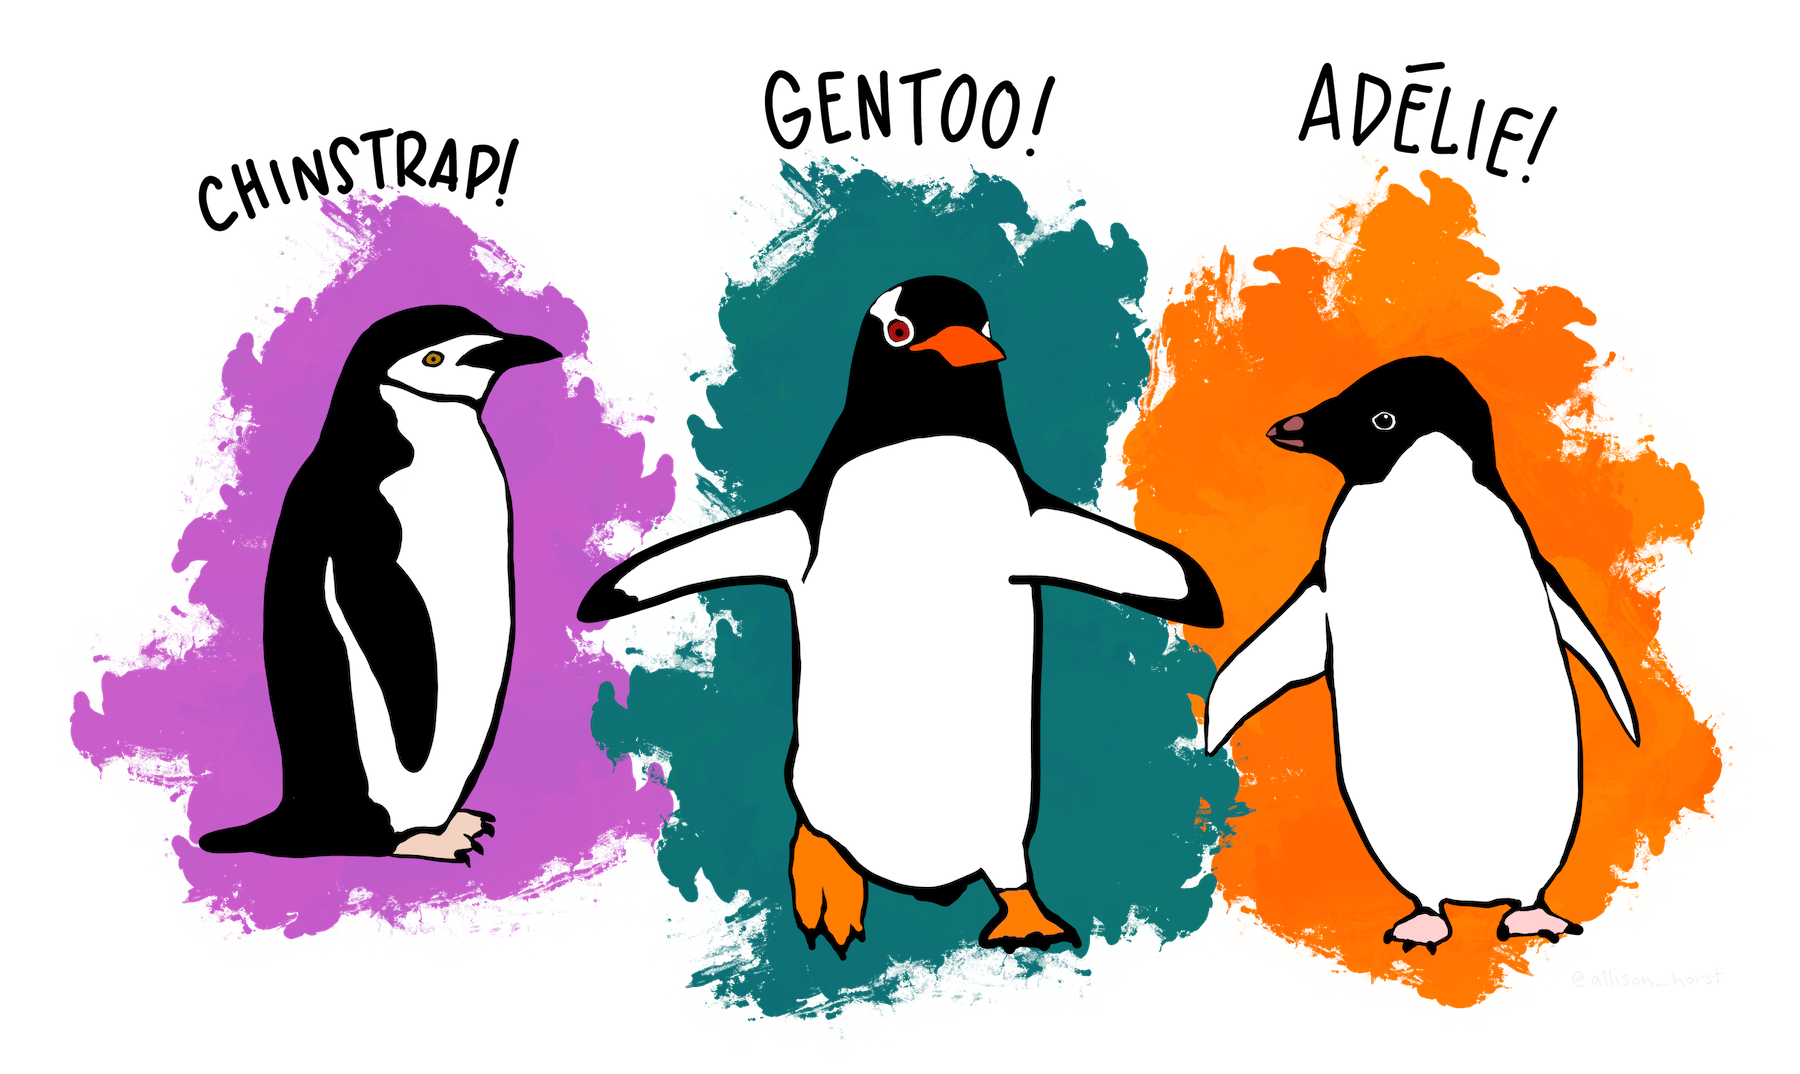
\includegraphics{images/Penguins.png}

}

\caption{\label{fig-ppenguins}Les 3 espèces de manchots de l'archipel de
Palmer. Illustration : Allison Horst}

\end{figure}%

\section{\texorpdfstring{Le data frame
\texttt{penguins}}{Le data frame penguins}}\label{le-data-frame-penguins}

Nous allons commencer par explorer le jeu de données \texttt{penguins}
qui est inclus avec le package \texttt{palmerpenguins} afin de nous
faire une idée de sa structure. Dans votre script, tapez la commande
suivante et exécutez la dans la console (selon les réglages de
\texttt{RStudio} et \emph{la largeur de votre console}, l'affichage peut
varier légèrement) :

\begin{Shaded}
\begin{Highlighting}[]
\NormalTok{penguins}
\end{Highlighting}
\end{Shaded}

\begin{verbatim}
# A tibble: 344 x 8
   species island    bill_length_mm bill_depth_mm flipper_length_mm body_mass_g
   <fct>   <fct>              <dbl>         <dbl>             <int>       <int>
 1 Adelie  Torgersen           39.1          18.7               181        3750
 2 Adelie  Torgersen           39.5          17.4               186        3800
 3 Adelie  Torgersen           40.3          18                 195        3250
 4 Adelie  Torgersen           NA            NA                  NA          NA
 5 Adelie  Torgersen           36.7          19.3               193        3450
 6 Adelie  Torgersen           39.3          20.6               190        3650
 7 Adelie  Torgersen           38.9          17.8               181        3625
 8 Adelie  Torgersen           39.2          19.6               195        4675
 9 Adelie  Torgersen           34.1          18.1               193        3475
10 Adelie  Torgersen           42            20.2               190        4250
# i 334 more rows
# i 2 more variables: sex <fct>, year <int>
\end{verbatim}

Essayons de décrypter cet affichage :

\begin{itemize}
\tightlist
\item
  \texttt{A\ tibble:\ 344\ x\ 8} : un tibble est un \texttt{data.frame}
  amélioré. Il a toutes les caractéristiques d'un \texttt{data.frame},
  (tapez \texttt{class(penguins)} pour vous en convaincre), mais en
  plus, il a quelques propriétés intéressantes sur lesquelles nous
  reviendrons plus tard. Ce \texttt{tibble} possède donc :

  \begin{itemize}
  \tightlist
  \item
    344 lignes
  \item
    8 colonnes, qui correspondent aux variables. Dans un
    \texttt{tibble}, les observations sont toujours en lignes et les
    variables en colonnes
  \end{itemize}
\item
  \texttt{species}, \texttt{island}, \texttt{bill\_length\_mm},
  \texttt{bill\_depth\_mm}, \texttt{flipper\_length\_mm}\ldots{} sont
  les noms des colonnes, c'est à dire les variables de ce jeu de données
\item
  Nous avons ensuite les 10 premières lignes du tableau
\item
  \texttt{...\ with\ 334\ more\ rows,\ and\ abbreviated\ variable\ names...},
  nous indique que 334 lignes ne logent pas à l'écran et que le nom de
  certains variables a été abrégé afin de permettre un affichage plus
  clair. Ces données font toutefois partie intégrante du tableau
  \texttt{penguins}
\item
  les noms complets de toutes les variables abrégées sont également
  indiqués
\end{itemize}

Cette façon d'afficher les tableaux est spécifique des \texttt{tibble}s.
Vous noterez que le type de chaque variable est indiqué entre
\texttt{\textless{}...\textgreater{}}, juste sous les noms de colonnes.
Voici certains des types de données que vous pourrez rencontrer :

\begin{itemize}
\tightlist
\item
  \texttt{\textless{}int\textgreater{}} : nombres entiers (``integers'')
\item
  \texttt{\textless{}dbl\textgreater{}} : nombres réels (``doubles'')
\item
  \texttt{\textless{}chr\textgreater{}} : caractères (``characters'')
\item
  \texttt{\textless{}fct\textgreater{}} : facteurs (``factors'')
\item
  \texttt{\textless{}ord\textgreater{}} : facteurs ordonnés
  (``ordinals'')
\item
  \texttt{\textless{}lgl\textgreater{}} : logiques (colonne de
  vrais/faux : ``logical'')
\item
  \texttt{\textless{}date\textgreater{}} : dates
\item
  \texttt{\textless{}time\textgreater{}} : heures
\item
  \texttt{\textless{}dttm\textgreater{}} : combinaison de date et
  d'heure (``date time'')
\end{itemize}

Cette façon d'afficher le contenu d'un tableau permet d'y voir
(beaucoup) plus clair que l'affichage classique d'un
\texttt{data.frame}. Malheureusement, ce n'est pas toujours suffisant.
Voyons quelles sont les autres méthodes permettant d'explorer un
\texttt{data.frame}.

\section{\texorpdfstring{Explorer un
\texttt{data.frame}}{Explorer un data.frame}}\label{explorer-un-data.frame}

Parmi les nombreuses façons d'avoir une idée des données contenues dans
un \texttt{data.frame} tel que \texttt{penguins}, on présente ici 3
fonctions qui prennent le nom du \texttt{data.frame} en guise
d'argument, et un opérateur :

\begin{itemize}
\tightlist
\item
  la fonction \texttt{View()} intégrée à \texttt{RStudio}. C'est celle
  que vous utiliserez le plus souvent. Attention, elle s'écrit avec un
  ``V'' majuscule
\item
  la fonction \texttt{glimpse()} chargée avec le package \texttt{dplyr}.
  Elle est très similaire à la fonction \texttt{str()} découverte dans
  les tutoriels de DataCamp
\item
  l'opérateur \texttt{\$} permet d'accéder à une unique variable d'un
  \texttt{data.frame}
\item
  la fonction \texttt{skim()} du package \texttt{skimr} permet d'obtenir
  un résumé complet mais très synthétique et visuel des variables d'un
  \texttt{data.frame}
\end{itemize}

\subsection{\texorpdfstring{\texttt{View()}}{View()}}\label{sec-view}

Tapez \texttt{View(penguins)} dans votre script et exécutez la commande.
Un nouvel onglet contenant ce qui ressemble à un tableur doit s'ouvrir.

\begin{tcolorbox}[enhanced jigsaw, colbacktitle=quarto-callout-tip-color!10!white, colframe=quarto-callout-tip-color-frame, bottomtitle=1mm, opacityback=0, arc=.35mm, leftrule=.75mm, titlerule=0mm, colback=white, title=\textcolor{quarto-callout-tip-color}{\faLightbulb}\hspace{0.5em}{Quizz : à quoi correspondent chacune des lignes de ce tableau ?}, toptitle=1mm, breakable, coltitle=black, rightrule=.15mm, left=2mm, opacitybacktitle=0.6, toprule=.15mm, bottomrule=.15mm]

\begin{enumerate}
\def\labelenumi{\alph{enumi}.}
\tightlist
\item
  aux données d'une espèce
\item
  aux données d'une île
\item
  aux données d'un individu
\item
  aux données d'une population (plusieurs manchots à la fois)
\end{enumerate}

\end{tcolorbox}

Ici, vous pouvez donc explorer la totalité du tableau, passer chaque
variable en revue, et même appliquer des filtres pour ne visualiser
qu'une partie des données. Par exemple, essayez de déterminer combien
d'individus sont issus de l'île ``Biscoe''.

Ce tableau n'est pas facile à manipuler. Il est impossible de corriger
des valeurs, et lorsque l'on applique des filtres, il est impossible de
récupérer uniquement les données filtrées. Nous verrons plus tard
comment les obtenir en tapant des commandes simples dans un script. La
seule utilité de ce tableau est donc l'exploration visuelle des données.

\subsection{\texorpdfstring{\texttt{glimpse()}}{glimpse()}}\label{glimpse}

La seconde façon d'explorer les données contenues dans un tableau est
d'utiliser la fonction \texttt{glimpse()} après avoir chargé le package
\texttt{dplyr} :

\begin{Shaded}
\begin{Highlighting}[]
\FunctionTok{glimpse}\NormalTok{(penguins)}
\end{Highlighting}
\end{Shaded}

\begin{verbatim}
Rows: 344
Columns: 8
$ species           <fct> Adelie, Adelie, Adelie, Adelie, Adelie, Adelie, Adel~
$ island            <fct> Torgersen, Torgersen, Torgersen, Torgersen, Torgerse~
$ bill_length_mm    <dbl> 39.1, 39.5, 40.3, NA, 36.7, 39.3, 38.9, 39.2, 34.1, ~
$ bill_depth_mm     <dbl> 18.7, 17.4, 18.0, NA, 19.3, 20.6, 17.8, 19.6, 18.1, ~
$ flipper_length_mm <int> 181, 186, 195, NA, 193, 190, 181, 195, 193, 190, 186~
$ body_mass_g       <int> 3750, 3800, 3250, NA, 3450, 3650, 3625, 4675, 3475, ~
$ sex               <fct> male, female, female, NA, female, male, female, male~
$ year              <int> 2007, 2007, 2007, 2007, 2007, 2007, 2007, 2007, 2007~
\end{verbatim}

Ici, les premières observations sont présentées en lignes pour chaque
variable du jeu de données. Là encore, le type de chaque variable est
précisé. Essayez d'identifier 3 variables catégorielles. À quoi
correspondent-elles ? En quoi sont-elles différentes des variables
numériques ?

\subsection{\texorpdfstring{L'opérateur
\texttt{\$}}{L'opérateur \$}}\label{lopuxe9rateur}

L'opérateur \texttt{\$} permet d'accéder à une unique variable grâce à
son nom. Par exemple on peut accéder à toutes les données concernant les
noms d'espèces (variable \texttt{species} du tableau \texttt{penguins})
en tapant :

\begin{Shaded}
\begin{Highlighting}[]
\NormalTok{penguins}\SpecialCharTok{$}\NormalTok{species}
\end{Highlighting}
\end{Shaded}

\begin{verbatim}
  [1] Adelie    Adelie    Adelie    Adelie    Adelie    Adelie    Adelie   
  [8] Adelie    Adelie    Adelie    Adelie    Adelie    Adelie    Adelie   
 [15] Adelie    Adelie    Adelie    Adelie    Adelie    Adelie    Adelie   
 [22] Adelie    Adelie    Adelie    Adelie    Adelie    Adelie    Adelie   
 [29] Adelie    Adelie    Adelie    Adelie    Adelie    Adelie    Adelie   
 [36] Adelie    Adelie    Adelie    Adelie    Adelie    Adelie    Adelie   
 [43] Adelie    Adelie    Adelie    Adelie    Adelie    Adelie    Adelie   
 [50] Adelie    Adelie    Adelie    Adelie    Adelie    Adelie    Adelie   
 [57] Adelie    Adelie    Adelie    Adelie    Adelie    Adelie    Adelie   
 [64] Adelie    Adelie    Adelie    Adelie    Adelie    Adelie    Adelie   
 [71] Adelie    Adelie    Adelie    Adelie    Adelie    Adelie    Adelie   
 [78] Adelie    Adelie    Adelie    Adelie    Adelie    Adelie    Adelie   
 [85] Adelie    Adelie    Adelie    Adelie    Adelie    Adelie    Adelie   
 [92] Adelie    Adelie    Adelie    Adelie    Adelie    Adelie    Adelie   
 [99] Adelie    Adelie    Adelie    Adelie    Adelie    Adelie    Adelie   
[106] Adelie    Adelie    Adelie    Adelie    Adelie    Adelie    Adelie   
[113] Adelie    Adelie    Adelie    Adelie    Adelie    Adelie    Adelie   
[120] Adelie    Adelie    Adelie    Adelie    Adelie    Adelie    Adelie   
[127] Adelie    Adelie    Adelie    Adelie    Adelie    Adelie    Adelie   
[134] Adelie    Adelie    Adelie    Adelie    Adelie    Adelie    Adelie   
[141] Adelie    Adelie    Adelie    Adelie    Adelie    Adelie    Adelie   
[148] Adelie    Adelie    Adelie    Adelie    Adelie    Gentoo    Gentoo   
[155] Gentoo    Gentoo    Gentoo    Gentoo    Gentoo    Gentoo    Gentoo   
[162] Gentoo    Gentoo    Gentoo    Gentoo    Gentoo    Gentoo    Gentoo   
[169] Gentoo    Gentoo    Gentoo    Gentoo    Gentoo    Gentoo    Gentoo   
[176] Gentoo    Gentoo    Gentoo    Gentoo    Gentoo    Gentoo    Gentoo   
[183] Gentoo    Gentoo    Gentoo    Gentoo    Gentoo    Gentoo    Gentoo   
[190] Gentoo    Gentoo    Gentoo    Gentoo    Gentoo    Gentoo    Gentoo   
[197] Gentoo    Gentoo    Gentoo    Gentoo    Gentoo    Gentoo    Gentoo   
[204] Gentoo    Gentoo    Gentoo    Gentoo    Gentoo    Gentoo    Gentoo   
[211] Gentoo    Gentoo    Gentoo    Gentoo    Gentoo    Gentoo    Gentoo   
[218] Gentoo    Gentoo    Gentoo    Gentoo    Gentoo    Gentoo    Gentoo   
[225] Gentoo    Gentoo    Gentoo    Gentoo    Gentoo    Gentoo    Gentoo   
[232] Gentoo    Gentoo    Gentoo    Gentoo    Gentoo    Gentoo    Gentoo   
[239] Gentoo    Gentoo    Gentoo    Gentoo    Gentoo    Gentoo    Gentoo   
[246] Gentoo    Gentoo    Gentoo    Gentoo    Gentoo    Gentoo    Gentoo   
[253] Gentoo    Gentoo    Gentoo    Gentoo    Gentoo    Gentoo    Gentoo   
[260] Gentoo    Gentoo    Gentoo    Gentoo    Gentoo    Gentoo    Gentoo   
[267] Gentoo    Gentoo    Gentoo    Gentoo    Gentoo    Gentoo    Gentoo   
[274] Gentoo    Gentoo    Gentoo    Chinstrap Chinstrap Chinstrap Chinstrap
[281] Chinstrap Chinstrap Chinstrap Chinstrap Chinstrap Chinstrap Chinstrap
[288] Chinstrap Chinstrap Chinstrap Chinstrap Chinstrap Chinstrap Chinstrap
[295] Chinstrap Chinstrap Chinstrap Chinstrap Chinstrap Chinstrap Chinstrap
[302] Chinstrap Chinstrap Chinstrap Chinstrap Chinstrap Chinstrap Chinstrap
[309] Chinstrap Chinstrap Chinstrap Chinstrap Chinstrap Chinstrap Chinstrap
[316] Chinstrap Chinstrap Chinstrap Chinstrap Chinstrap Chinstrap Chinstrap
[323] Chinstrap Chinstrap Chinstrap Chinstrap Chinstrap Chinstrap Chinstrap
[330] Chinstrap Chinstrap Chinstrap Chinstrap Chinstrap Chinstrap Chinstrap
[337] Chinstrap Chinstrap Chinstrap Chinstrap Chinstrap Chinstrap Chinstrap
[344] Chinstrap
Levels: Adelie Chinstrap Gentoo
\end{verbatim}

Cela nous permet de récupérer les données sous la forme d'un vecteur ou,
comme ici, d'un facteur. Attention toutefois, le tableau
\texttt{penguins} contient beaucoup de lignes. Récupérer une variable
grâce à cet opérateur peut rapidement saturer la console. Nous serons
amenés à manipuler des tableaux contenant plusieurs dizaines ou
centaines de milliers de lignes. C'est le cas du tableau
\texttt{diamonds} du package \texttt{ggplot2} que vous avez découvert
dans les exercice de la Section~\ref{sec-exo-1}.

Si, par exemple, vous souhaitez extraire les données relatives à la
clarté des diamants (colonne \texttt{clarity}) du tableau
\texttt{diamonds}, vous pouvez taper ceci :

\begin{Shaded}
\begin{Highlighting}[]
\FunctionTok{library}\NormalTok{(ggplot2)}
\NormalTok{diamonds}\SpecialCharTok{$}\NormalTok{clarity}
\end{Highlighting}
\end{Shaded}

Le résultat est pour le moins indigeste ! Lorsqu'un tableau contient de
nombreuses lignes, c'est rarement une bonne idée de transformer l'une de
ses colonnes en vecteur. Dans la mesure du possible, les données d'un
tableau doivent rester dans le tableau.

\subsection{\texorpdfstring{\texttt{skim()}}{skim()}}\label{skim}

Pour utiliser la fonction \texttt{skim()}, vous devez au préalable
installer le package \texttt{skimr} :

\begin{Shaded}
\begin{Highlighting}[]
\FunctionTok{install.packages}\NormalTok{(}\StringTok{"skimr"}\NormalTok{)}
\end{Highlighting}
\end{Shaded}

Ce package est un peu ``expérimental'' et il se peut que l'installation
pose problème. Si un message d'erreur apparaît lors de l'installation,
procédez comme suit :

\begin{enumerate}
\def\labelenumi{\arabic{enumi}.}
\tightlist
\item
  Quittez \texttt{RStudio} (sans oublier de sauvegarder votre travail au
  préalable)
\item
  Relancez \texttt{RStudio} et dans la console, tapez ceci :
\end{enumerate}

\begin{Shaded}
\begin{Highlighting}[]
\FunctionTok{install.packages}\NormalTok{(}\StringTok{"rlang"}\NormalTok{)}
\end{Highlighting}
\end{Shaded}

\begin{enumerate}
\def\labelenumi{\arabic{enumi}.}
\setcounter{enumi}{2}
\tightlist
\item
  Tentez d'installer \texttt{skimr} à nouveau.
\item
  Exécutez à nouveau tout votre script afin de retrouver votre travail
  dans l'état où il était avant de quitter \texttt{RStudio}.
\end{enumerate}

Si l'installation de \texttt{skimr} s'est bien passée, vous pouvez
maintenant taper ceci :

\begin{Shaded}
\begin{Highlighting}[]
\FunctionTok{library}\NormalTok{(skimr)}
\FunctionTok{skim}\NormalTok{(penguins)}
\end{Highlighting}
\end{Shaded}

\begin{longtable}[]{@{}ll@{}}
\caption{Data summary}\tabularnewline
\toprule\noalign{}
\endfirsthead
\endhead
\bottomrule\noalign{}
\endlastfoot
Name & penguins \\
Number of rows & 344 \\
Number of columns & 8 \\
\_\_\_\_\_\_\_\_\_\_\_\_\_\_\_\_\_\_\_\_\_\_\_ & \\
Column type frequency: & \\
factor & 3 \\
numeric & 5 \\
\_\_\_\_\_\_\_\_\_\_\_\_\_\_\_\_\_\_\_\_\_\_\_\_ & \\
Group variables & None \\
\end{longtable}

\textbf{Variable type: factor}

\begin{longtable}[]{@{}
  >{\raggedright\arraybackslash}p{(\columnwidth - 10\tabcolsep) * \real{0.1687}}
  >{\raggedleft\arraybackslash}p{(\columnwidth - 10\tabcolsep) * \real{0.1205}}
  >{\raggedleft\arraybackslash}p{(\columnwidth - 10\tabcolsep) * \real{0.1687}}
  >{\raggedright\arraybackslash}p{(\columnwidth - 10\tabcolsep) * \real{0.0964}}
  >{\raggedleft\arraybackslash}p{(\columnwidth - 10\tabcolsep) * \real{0.1084}}
  >{\raggedright\arraybackslash}p{(\columnwidth - 10\tabcolsep) * \real{0.3373}}@{}}
\toprule\noalign{}
\begin{minipage}[b]{\linewidth}\raggedright
skim\_variable
\end{minipage} & \begin{minipage}[b]{\linewidth}\raggedleft
n\_missing
\end{minipage} & \begin{minipage}[b]{\linewidth}\raggedleft
complete\_rate
\end{minipage} & \begin{minipage}[b]{\linewidth}\raggedright
ordered
\end{minipage} & \begin{minipage}[b]{\linewidth}\raggedleft
n\_unique
\end{minipage} & \begin{minipage}[b]{\linewidth}\raggedright
top\_counts
\end{minipage} \\
\midrule\noalign{}
\endhead
\bottomrule\noalign{}
\endlastfoot
species & 0 & 1.00 & FALSE & 3 & Ade: 152, Gen: 124, Chi: 68 \\
island & 0 & 1.00 & FALSE & 3 & Bis: 168, Dre: 124, Tor: 52 \\
sex & 11 & 0.97 & FALSE & 2 & mal: 168, fem: 165 \\
\end{longtable}

\textbf{Variable type: numeric}

\begin{longtable}[]{@{}
  >{\raggedright\arraybackslash}p{(\columnwidth - 20\tabcolsep) * \real{0.1800}}
  >{\raggedleft\arraybackslash}p{(\columnwidth - 20\tabcolsep) * \real{0.1000}}
  >{\raggedleft\arraybackslash}p{(\columnwidth - 20\tabcolsep) * \real{0.1400}}
  >{\raggedleft\arraybackslash}p{(\columnwidth - 20\tabcolsep) * \real{0.0800}}
  >{\raggedleft\arraybackslash}p{(\columnwidth - 20\tabcolsep) * \real{0.0700}}
  >{\raggedleft\arraybackslash}p{(\columnwidth - 20\tabcolsep) * \real{0.0700}}
  >{\raggedleft\arraybackslash}p{(\columnwidth - 20\tabcolsep) * \real{0.0800}}
  >{\raggedleft\arraybackslash}p{(\columnwidth - 20\tabcolsep) * \real{0.0800}}
  >{\raggedleft\arraybackslash}p{(\columnwidth - 20\tabcolsep) * \real{0.0700}}
  >{\raggedleft\arraybackslash}p{(\columnwidth - 20\tabcolsep) * \real{0.0700}}
  >{\raggedright\arraybackslash}p{(\columnwidth - 20\tabcolsep) * \real{0.0600}}@{}}
\toprule\noalign{}
\begin{minipage}[b]{\linewidth}\raggedright
skim\_variable
\end{minipage} & \begin{minipage}[b]{\linewidth}\raggedleft
n\_missing
\end{minipage} & \begin{minipage}[b]{\linewidth}\raggedleft
complete\_rate
\end{minipage} & \begin{minipage}[b]{\linewidth}\raggedleft
mean
\end{minipage} & \begin{minipage}[b]{\linewidth}\raggedleft
sd
\end{minipage} & \begin{minipage}[b]{\linewidth}\raggedleft
p0
\end{minipage} & \begin{minipage}[b]{\linewidth}\raggedleft
p25
\end{minipage} & \begin{minipage}[b]{\linewidth}\raggedleft
p50
\end{minipage} & \begin{minipage}[b]{\linewidth}\raggedleft
p75
\end{minipage} & \begin{minipage}[b]{\linewidth}\raggedleft
p100
\end{minipage} & \begin{minipage}[b]{\linewidth}\raggedright
hist
\end{minipage} \\
\midrule\noalign{}
\endhead
\bottomrule\noalign{}
\endlastfoot
bill\_length\_mm & 2 & 0.99 & 43.92 & 5.46 & 32.1 & 39.23 & 44.45 & 48.5
& 59.6 & ▃▇▇▆▁ \\
bill\_depth\_mm & 2 & 0.99 & 17.15 & 1.97 & 13.1 & 15.60 & 17.30 & 18.7
& 21.5 & ▅▅▇▇▂ \\
flipper\_length\_mm & 2 & 0.99 & 200.92 & 14.06 & 172.0 & 190.00 &
197.00 & 213.0 & 231.0 & ▂▇▃▅▂ \\
body\_mass\_g & 2 & 0.99 & 4201.75 & 801.95 & 2700.0 & 3550.00 & 4050.00
& 4750.0 & 6300.0 & ▃▇▆▃▂ \\
year & 0 & 1.00 & 2008.03 & 0.82 & 2007.0 & 2007.00 & 2008.00 & 2009.0 &
2009.0 & ▇▁▇▁▇ \\
\end{longtable}

Nous aurons l'occasion de revenir en détail sur la signification de tous
ces indices à la Section~\ref{sec-skim}. À ce stade, retenez que cette
fonction \texttt{skim()} permet d'accéder à un résumé très détaillé de
chaque variable d'un jeu de données. Par exemple, on apprend ici que la
masse corporelle moyenne des manchots de l'ensemble du jeu de données
vaut 4201.75 grammes (ligne \texttt{body\_mass\_g}, colonne
\texttt{mean}), avec un écart-type de 0.82 grammes (colonne
\texttt{sd}), et que la masse de 2 individus est manquante (colonne
\texttt{n\_missing}). Cette fonction nous sera donc très utile lorsque
nous aborderons la question des statistiques descriptives.

\subsection{Les fichiers d'aide}\label{les-fichiers-daide}

Une fonctionnalité particulièrement utile de \texttt{R} est son système
d'aide. On peut obtenir de l'aide au sujet de n'importe quelle fonction
et de n'importe quel jeu de données en tapant un ``\texttt{?}''
immédiatement suivi du nom de la fonction ou de l'objet.

Par exemple, examinez l'aide du jeu de données \texttt{penguins} :

\begin{Shaded}
\begin{Highlighting}[]
\NormalTok{?penguins}
\end{Highlighting}
\end{Shaded}

Vous devriez absolument prendre l'habitude d'examiner les fichiers
d'aide des fonctions ou jeux de données pour lesquels vous avez des
questions. Ces fichiers sont très complets, et même s'il peuvent
paraître impressionnants au premier abord, ils sont tous structurés sur
le même modèle et vous aideront à comprendre comment utiliser les
fonctions, quels sont les arguments possibles, à quoi ils servent et
comment les utiliser.

Prenez le temps d'examiner le fichier d'aide du jeu de données
\texttt{penguins}. Avant de passer à la suite, assurez-vous d'avoir
compris à quoi correspondent chacune des 8 variables de ce tableau.

\section{Exercices}\label{sec-exo-2}

Consultez l'aide du jeu de données \texttt{diamonds} du package
\texttt{ggplot2}.

\begin{itemize}
\tightlist
\item
  Quel est le code de la couleur la plus prisée ?
\item
  Quel est le code de la moins bonne clarté ?
\item
  À quoi correspond la variable \texttt{z} ?
\item
  En quoi la variable \texttt{depth} est-elle différente de la variable
  \texttt{z} ?
\end{itemize}

Installez le package \texttt{nycflights13} et consultez son aide en
tapant \texttt{help(package="nycflights13")}.

\begin{itemize}
\tightlist
\item
  Consultez l'aide des 5 jeux de données de ce package.
\item
  À quoi correspond la variable \texttt{visib} ?
\item
  Dans quel tableau se trouve-t-elle ?
\item
  Combien de lignes possède ce tableau ?
\end{itemize}

\bookmarksetup{startatroot}

\chapter{\texorpdfstring{Visualiser des données avec
\texttt{ggplot2}}{Visualiser des données avec ggplot2}}\label{sec-viz}

\section{Préambule}\label{pruxe9ambule-2}

Dans le Chapitre~\ref{sec-basics} et le Chapitre~\ref{sec-dataset}, vous
avez découvert les concepts essentiels qu'il est important de maîtriser
avant de commencer à explorer en détail des données dans \texttt{R}. Les
éléments de syntaxe abordés dans la Section~\ref{sec-code} sont nombreux
et vous n'avez probablement pas tout retenu. C'est pourquoi je vous
conseille de garder les tutoriels de DataCamp à portée de main afin de
pouvoir refaire les parties que vous maîtrisez le moins. Ce n'est qu'en
répétant plusieurs fois ces tutoriels que les choses seront vraiment
comprises et que vous les retiendrez. Ainsi, si des éléments de code
présentés ci-dessous vous semblent obscurs, revenez en arrière : toutes
les réponses à vos questions se trouvent probablement dans les chapitres
précédents.

Après la découverte des bases du langage \texttt{R}, nous abordons
maintenant les parties de ce livre qui concernent la ``science des
données'' (ou ``Data Science'' pour nos amis anglo-saxons). Nous allons
voir dans ce chapitre qu'outre les fonctions \texttt{View()} et
\texttt{glimpse()}, l'exploration visuelle \emph{via} la représentation
graphique des données est un moyen indispensable et très puissant pour
comprendre ce qui se passe dans un jeu de données.

\begin{tcolorbox}[enhanced jigsaw, colbacktitle=quarto-callout-important-color!10!white, colframe=quarto-callout-important-color-frame, bottomtitle=1mm, opacityback=0, arc=.35mm, leftrule=.75mm, titlerule=0mm, colback=white, title=\textcolor{quarto-callout-important-color}{\faExclamation}\hspace{0.5em}{Important}, toptitle=1mm, breakable, coltitle=black, rightrule=.15mm, left=2mm, opacitybacktitle=0.6, toprule=.15mm, bottomrule=.15mm]

La visualisation de vos données est un \textbf{préalable indispensable}
à toute analyse statistique.

\end{tcolorbox}

La visualisation des données est en outre un excellent point de départ
quand on découvre la programmation sous \texttt{R}, car ses bénéfices
sont clairs et immédiats : vous pouvez créer des graphiques élégants et
informatifs qui vous aident à comprendre les données. Dans ce chapitre,
vous allez donc plonger dans l'art de la visualisation des données, en
apprenant la structure de base des graphiques réalisés avec
\texttt{ggplot2} qui permettent de transformer des données numériques et
catégorielles en graphiques.

Toutefois, la visualisation seule ne suffit généralement pas. Il est en
effet souvent nécessaire de transformer les données pour produire des
représentations plus parlantes. Ainsi, dans le
Chapitre~\ref{sec-wrangling}, vous découvrirez les fonctions clés qui
vous permettront de sélectionner des variables importantes, de filtrer
des observations, de créer de nouvelles variables, ou d'en modifier la
forme.

Ce n'est qu'en combinant les transformations de données et
représentations graphiques d'une part, avec votre curiosité et votre
esprit critique d'autre part, que vous serez véritablement en mesure de
réaliser une analyse exploratoire de vos données à la fois utile et
pertinente. C'est la seule façon d'identifier des questions
intéressantes sur vos données, afin de tenter d'y répondre par les
analyses statistiques et la modélisation.

\section{Prérequis}\label{pruxe9requis}

Dans ce chapitre, nous aurons besoin des packages suivants :

\begin{Shaded}
\begin{Highlighting}[]
\FunctionTok{library}\NormalTok{(tidyverse)}
\FunctionTok{library}\NormalTok{(palmerpenguins)}
\FunctionTok{library}\NormalTok{(nycflights13)}
\FunctionTok{library}\NormalTok{(gapminder)}
\FunctionTok{library}\NormalTok{(scales)}
\end{Highlighting}
\end{Shaded}

Si ce n'est pas déjà fait, pensez à les installer avant de les charger
en mémoire.

Au niveau le plus élémentaire, les graphiques permettent de comprendre
comment les variables se comparent en termes de tendance centrale (à
quel endroit les valeurs ont tendance à être localisées, regroupées) et
leur dispersion (comment les données varient autour du centre). La chose
la plus importante à savoir sur les graphiques est qu'ils doivent être
créés pour que votre public (le professeur qui vous évalue, le collègue
avec qui vous collaborez, votre futur employeur, etc.) comprenne bien
les résultats et les informations que vous souhaitez transmettre. Il
s'agit d'un exercice d'équilibriste : d'une part, vous voulez mettre en
évidence autant de relations significatives et de résultats intéressants
que possible, mais de l'autre, vous ne voulez pas trop en inclure, afin
d'éviter de rendre votre graphique illisible ou de submerger votre
public. Tout comme n'importe quel paragraphe de document écrit, un
graphique doit permettre de \textbf{communiquer un message} (une idée
forte, un résultat marquant, une hypothèse nouvelle, etc).

Comme nous le verrons, les graphiques nous aident également à repérer
les tendances extrêmes et les valeurs aberrantes dans nos données. Nous
verrons aussi qu'une façon de faire, assez classique, consiste à
comparer la distribution d'une variable quantitative pour les différents
niveaux d'une variable catégorielle.

\begin{tcolorbox}[enhanced jigsaw, colbacktitle=quarto-callout-tip-color!10!white, colframe=quarto-callout-tip-color-frame, bottomtitle=1mm, opacityback=0, arc=.35mm, leftrule=.75mm, titlerule=0mm, colback=white, title=\textcolor{quarto-callout-tip-color}{\faLightbulb}\hspace{0.5em}{Objectifs}, toptitle=1mm, breakable, coltitle=black, rightrule=.15mm, left=2mm, opacitybacktitle=0.6, toprule=.15mm, bottomrule=.15mm]

Dans ce chapitre, vous apprendrez à :

\begin{enumerate}
\def\labelenumi{\arabic{enumi}.}
\tightlist
\item
  faire différents types de graphiques exploratoires avec le package
  \texttt{ggplot2} \faIcon{chart-line} \faIcon{chart-bar}
  \faIcon{chart-area}
\item
  choisir le ou les graphiques appropriés selon la nature des variables
  dont vous disposez ou que vous souhaitez mettre en relation
\item
  mettre vos graphiques en forme pour les intégrer dans vos rapports ou
  compte-rendus de TP
\end{enumerate}

\end{tcolorbox}

\section{La grammaire des graphiques}\label{sec-gggraph}

Les lettres \texttt{gg} du package \texttt{ggplot2} sont l'abréviation
de ``\textbf{g}rammar of \textbf{g}raphics'' : la grammaire des
graphiques. De la même manière que nous construisons des phrases en
respectant des règles grammaticales précises (usage des noms, des
verbes, des sujets et adjectifs\ldots), la grammaire des graphiques
établit un certain nombre de règles permettant de construire des
graphiques : elle précise les composants d'un graphique en suivant le
cadre théorique défini par Wilkinson (2005).

\subsection{Éléments de la
grammaire}\label{uxe9luxe9ments-de-la-grammaire}

En bref, la grammaire des graphiques nous dit que :

\begin{quote}
Un graphique est l'association (\texttt{mapping}) de données/variables
(\texttt{data}) à des attributs esthétiques (\texttt{aes}thetics)
d'objets géométriques (\texttt{geom}etric objects).
\end{quote}

Pour clarifier, on peut disséquer un graphique en 3 éléments essentiels
:

\begin{enumerate}
\def\labelenumi{\arabic{enumi}.}
\tightlist
\item
  \texttt{data} : le jeu de données contenant les variables que l'on va
  associer à des objets géométriques. Pour \texttt{ggplot2} les données
  doivent obligatoirement être stockées dans un \texttt{data.frame} ou
  un \texttt{tibble}
\item
  \texttt{geom} : les objets géométriques en question. Cela fait
  référence aux types d'objets que l'on peut observer sur le graphique
  (des points, des lignes, des barres, etc.)
\item
  \texttt{aes} : les attributs esthétiques des objets géométriques
  présents sur le graphique. Par exemple, la position sur les axes
  \texttt{x} et \texttt{y}, la couleur, la taille, la transparence, la
  forme, etc. Chacun de ces attributs esthétiques peut-être associé à
  une variable de notre jeu de données.
\end{enumerate}

Examinons un exemple pour bien comprendre.

\subsection{Gapminder}\label{gapminder}

En février 2006, un statisticien du nom de Hans Rosling a donné un TED
Talk intitulé
``\href{https://www.ted.com/talks/hans_rosling_shows_the_best_stats_you_ve_ever_seen}{The
best stats you'we ever seen}''. Au cours de cette conférence, Hans
Rosling présente des données sur l'économie mondiale, la santé et le
développement des pays du monde. Les données sont disponibles
\href{https://www.gapminder.org/tools/\#$chart-type=bubbles}{sur ce
site} et dans
\href{https://cran.r-project.org/web/packages/gapminder/index.html}{le
package \texttt{gapminder}}.

Pour l'année 2007, le jeu de données contient des informations pour 142
pays. Examinons les premières lignes de ce jeu de données :

\begin{longtable}[]{@{}llrrr@{}}
\caption{Les 6 premières lignes du jeu de données \texttt{gapminder}
pour l'année 2007.}\tabularnewline
\toprule\noalign{}
Country & Continent & Life Expectancy & Population & GDP per Capita \\
\midrule\noalign{}
\endfirsthead
\toprule\noalign{}
Country & Continent & Life Expectancy & Population & GDP per Capita \\
\midrule\noalign{}
\endhead
\bottomrule\noalign{}
\endlastfoot
Afghanistan & Asia & 43.828 & 31889923 & 974.5803 \\
Albania & Europe & 76.423 & 3600523 & 5937.0295 \\
Algeria & Africa & 72.301 & 33333216 & 6223.3675 \\
Angola & Africa & 42.731 & 12420476 & 4797.2313 \\
Argentina & Americas & 75.320 & 40301927 & 12779.3796 \\
Australia & Oceania & 81.235 & 20434176 & 34435.3674 \\
\end{longtable}

Pour chaque ligne, les variables suivantes sont décrites :

\begin{itemize}
\tightlist
\item
  \texttt{Country} : le pays
\item
  \texttt{Continent} : le continent
\item
  \texttt{Life\ Expectancy} : espérance de vie à la naissance
\item
  \texttt{Population} : nombre de personnes vivant dans le pays
\item
  \texttt{GDP\ per\ Capita} : produit intérieur brut (PIB) par habitant
  en dollars américains. GDP est l'abréviation de ``Growth Domestic
  Product''. C'est un indicateur de l'activité économique d'un pays,
  parfois utilisé comme une approximation du revenu moyen par habitant.
\end{itemize}

Examinons maintenant la Figure~\ref{fig-gapminder} qui représente ces
variables pour chacun des 142 pays de ce jeu de données (notez
l'utilisation de la notation scientifique dans la légende, et de
l'échelle logarithmique de l'axe des abscisses).

\begin{figure}

\centering{

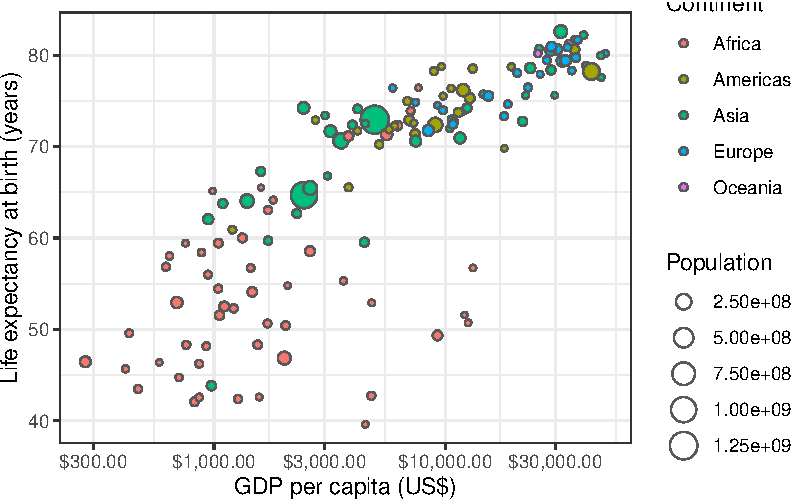
\includegraphics{03-Visualization_files/figure-pdf/fig-gapminder-1.pdf}

}

\caption{\label{fig-gapminder}Espérance de vie en fonction du PIB par
habitant en 2007.}

\end{figure}%

Si on décrypte ce graphique du point de vue de la grammaire des
graphiques, on voit que :

\begin{itemize}
\tightlist
\item
  la variable \texttt{GDP\ per\ Capita} est associée à
  l'\texttt{aes}thetic \texttt{x} de la position des points
\item
  la variable \texttt{Life\ Expectancy} est associée à
  l'\texttt{aes}thetic \texttt{y} de la position des points
\item
  la variable \texttt{Population} est associée à l'\texttt{aes}thetic
  \texttt{size} (taille) des points
\item
  la variable \texttt{Continent} est associée à l'\texttt{aes}thetic
  \texttt{color} (couleur) des points
\end{itemize}

Ici, l'objet géométrique (ou \texttt{geom}) qui représente les données
est le point. Les données (ou \texttt{data}) sont contenues dans le
tableau \texttt{gapminder} et chacune de ces variables est associée
(\texttt{mapping}) aux caractéristiques esthétiques des points.

\subsection{Autres éléments de la grammaire des
graphiques}\label{autres-uxe9luxe9ments-de-la-grammaire-des-graphiques}

Outre les éléments indispensables évoqués ici (\texttt{data},
\texttt{mapping}, \texttt{aes}, et \texttt{geom}), il existe d'autres
aspects de la grammaire des graphiques qui permettent de contrôler
l'aspect des graphiques. Ils ne sont pas toujours indispensables. Nous
en verrons néanmoins quelque-uns particulièrement utiles :

\begin{itemize}
\tightlist
\item
  \texttt{facet} : c'est un moyen très pratique de scinder le jeu de
  données en plusieurs sous-groupes et de produire automatiquement un
  graphique pour chacun d'entre eux.
\item
  \texttt{position} : permet notamment de modifier la position des
  barres d'un barplot.
\item
  \texttt{labs} : permet de définir les titres, sous-titres et légendes
  des axes d'un graphique
\item
  \texttt{theme} : permet de modifier l'apect général des graphiques en
  appliquant des thèmes prédéfinis ou en modifiant certains aspects de
  thèmes existants
\end{itemize}

\subsection{\texorpdfstring{Le package
\texttt{ggplot2}}{Le package ggplot2}}\label{le-package-ggplot2}

Comme indiqué plus haut, le package \texttt{ggplot2} (Wickham et al.
2024) permet de réaliser des graphiques dans \texttt{R} en respectant
les principes de la grammaire des graphiques. Vous avez probablement
remarqué que depuis le début de la section Section~\ref{sec-gggraph},
beaucoup de termes sont écrits dans la police réservée au \texttt{code}
informatique. C'est parce que les éléments de la grammaire des
graphiques sont tous précisés dans la fonction \texttt{ggplot()} qui
demande, au grand minimum, que les éléments suivants soient spécifiés :

\begin{itemize}
\tightlist
\item
  le nom du \texttt{data.frame} contenant les variables qui seront
  utilisées pour le graphique. Ce nom correspond à l'argument
  \texttt{data} de la fonction \texttt{ggplot()}.
\item
  l'association des variables à des attributs esthétiques. Cela se fait
  grâce à l'argument \texttt{mapping} et la fonction \texttt{aes()}
\end{itemize}

Après avoir spécifié ces éléments, on ajoute des couches supplémentaires
au graphique grâce au signe \texttt{+}. La couche la plus essentielle à
ajouter à un graphique, est une couche contenant un élément géométrique,
ou \texttt{geom} (par exemple des points, des lignes ou des barres).
D'autres couches peuvent s'ajouter pour spécifier des titres, des
\texttt{facet}s ou des modifications des axes et des thèmes du
graphique.

Dans le cadre de ce cours, nous verrons un grand nombre de types de
gra{[}hiques distincts, y compris les 5 types de graphiques les plus
courants :

\begin{enumerate}
\def\labelenumi{\arabic{enumi}.}
\tightlist
\item
  les nuages de points
\item
  les graphiques en lignes
\item
  les histogrammes
\item
  les diagrammes bâtons
\item
  les boîtes à moustaches
\end{enumerate}

\subsection{Votre premier graphique}\label{votre-premier-graphique}

Reprenons maintenant le jeu de données \texttt{penguins} :

\begin{Shaded}
\begin{Highlighting}[]
\NormalTok{penguins}
\end{Highlighting}
\end{Shaded}

\begin{verbatim}
# A tibble: 344 x 8
   species island    bill_length_mm bill_depth_mm flipper_length_mm body_mass_g
   <fct>   <fct>              <dbl>         <dbl>             <int>       <int>
 1 Adelie  Torgersen           39.1          18.7               181        3750
 2 Adelie  Torgersen           39.5          17.4               186        3800
 3 Adelie  Torgersen           40.3          18                 195        3250
 4 Adelie  Torgersen           NA            NA                  NA          NA
 5 Adelie  Torgersen           36.7          19.3               193        3450
 6 Adelie  Torgersen           39.3          20.6               190        3650
 7 Adelie  Torgersen           38.9          17.8               181        3625
 8 Adelie  Torgersen           39.2          19.6               195        4675
 9 Adelie  Torgersen           34.1          18.1               193        3475
10 Adelie  Torgersen           42            20.2               190        4250
# i 334 more rows
# i 2 more variables: sex <fct>, year <int>
\end{verbatim}

Comme évoqué plus haut, il s'agit d'un \texttt{tibble}. Plusieurs de ses
variables concernent la biométrie des manchots, en particulier de son
bec (voir Figure~\ref{fig-morpho}).

\begin{figure}

\centering{

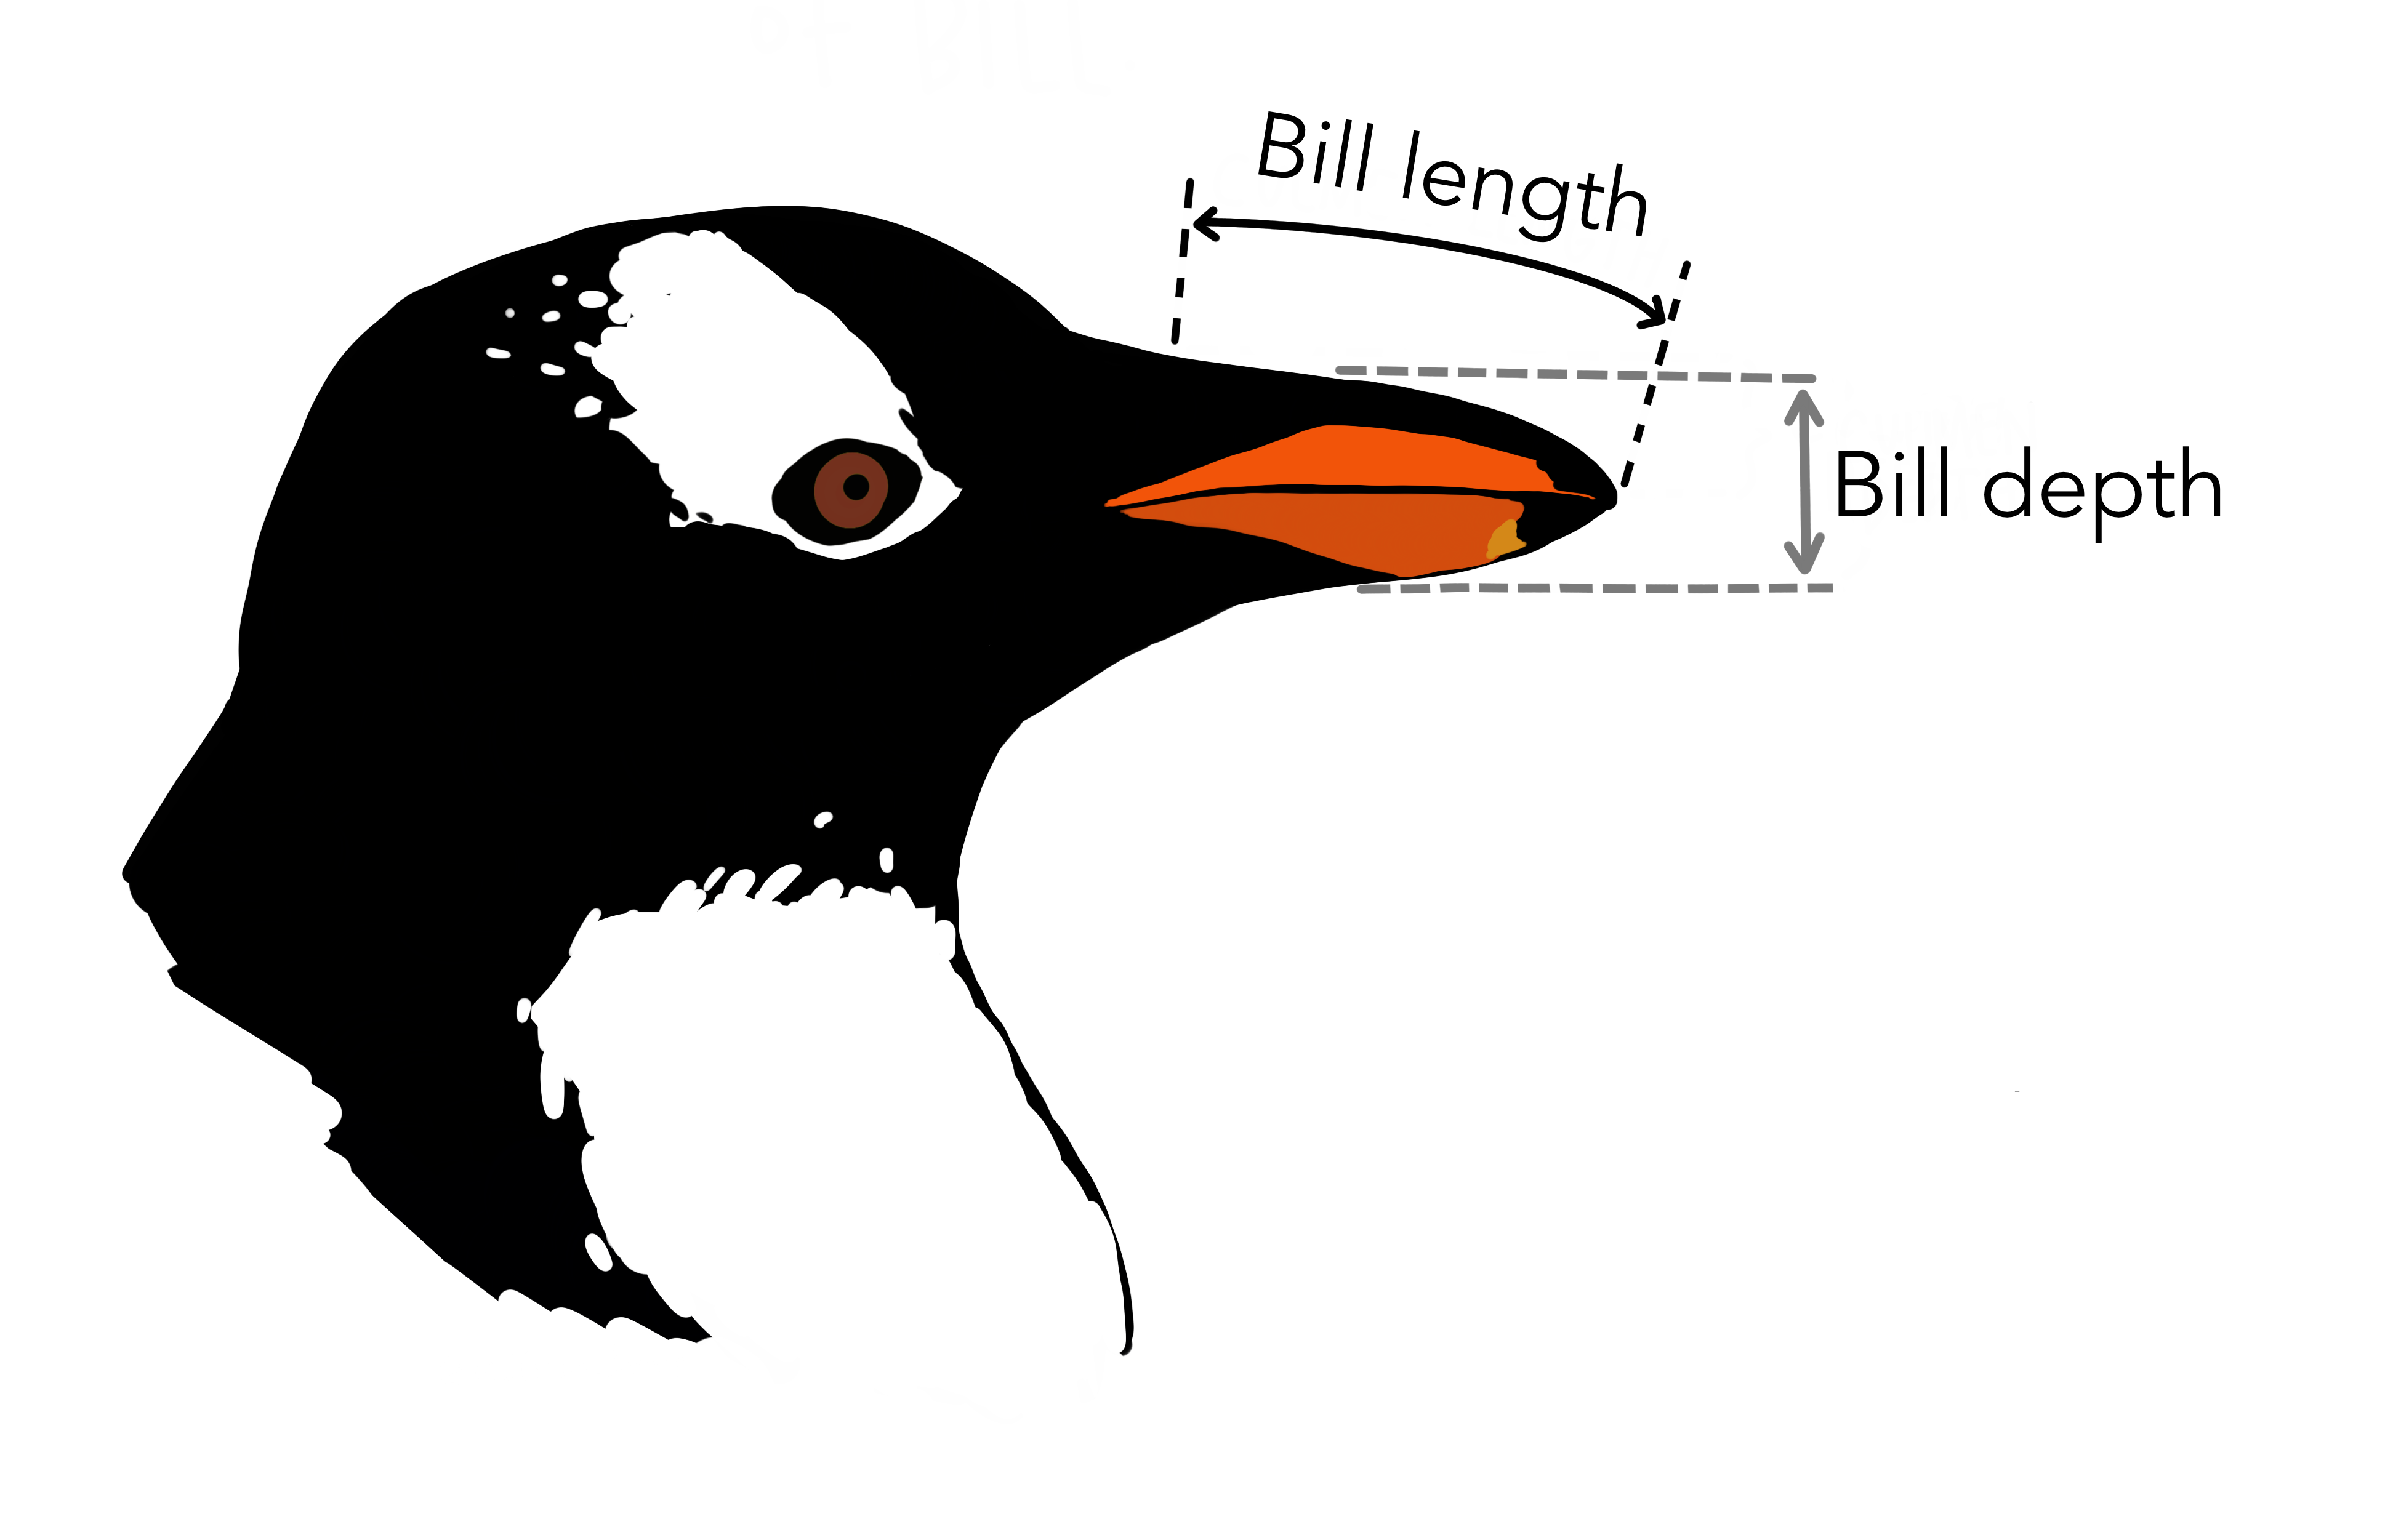
\includegraphics[width=0.5\textwidth,height=\textheight]{images/culmen_depth.png}

}

\caption{\label{fig-morpho}Morphométrie du bec des manchots.
Illustration de Allison Horst}

\end{figure}%

Supposons qu'on cherche à déterminer si la longueur du bec des manchots
est proportionnelle à leur masse. Pour produire un graphique permettant
de le déterminer, nous avons besoin des éléments suivants :

\begin{enumerate}
\def\labelenumi{\arabic{enumi}.}
\tightlist
\item
  \texttt{data} : le tableau \texttt{penguins}
\item
  un objet géométrique, ici, des points (\texttt{geom\_point()}) puisque
  nous disposons de 2 variables numériques (plus de détails à ce sujet
  plus bas)
\item
  l'association de certaines variables du jeu de données (ici,
  \texttt{body\_mass\_g} et \texttt{bill\_length\_mm}) à certaines
  caractéristiques esthétiques du graphiques (ici, la position sur les
  axes des \texttt{x} et des \texttt{y}), grâce à l'argument
  \texttt{mapping} et la fonction \texttt{aes()}.
\end{enumerate}

Concrètement, voilà le code qu'il faut taper dans votre script :

\begin{Shaded}
\begin{Highlighting}[]
\FunctionTok{ggplot}\NormalTok{(}\AttributeTok{data =}\NormalTok{ penguins, }\AttributeTok{mapping =} \FunctionTok{aes}\NormalTok{(}\AttributeTok{x =}\NormalTok{ body\_mass\_g, }\AttributeTok{y =}\NormalTok{ bill\_length\_mm))}
\end{Highlighting}
\end{Shaded}

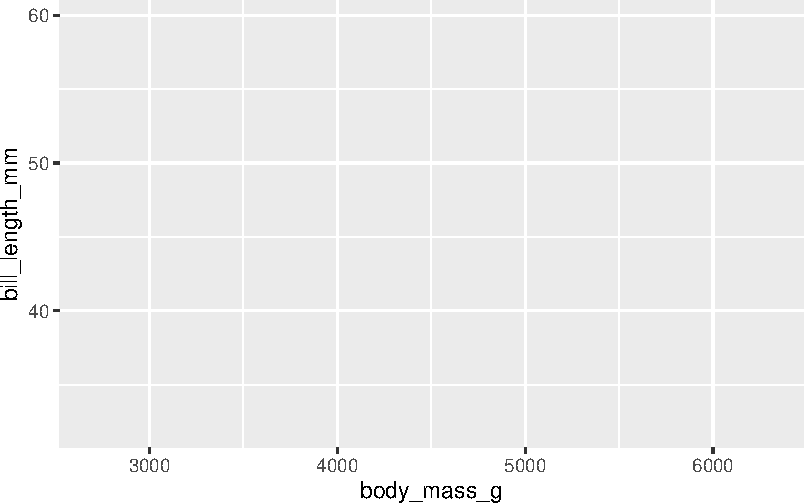
\includegraphics{03-Visualization_files/figure-pdf/unnamed-chunk-5-1.pdf}

Cette première ligne de code permet de faire plusieurs choses :

\begin{enumerate}
\def\labelenumi{\arabic{enumi}.}
\tightlist
\item
  on indique à \texttt{R} qu'on souhaite faire un graphique (avec la
  fonction \texttt{ggplot()})
\item
  on indique à \texttt{R} que les données sont contenues dans l'objet
  \texttt{penguins} avec \texttt{data\ =\ penguins}
\item
  on associe (avec \texttt{mapping\ =} la variable
  \texttt{body\_mass\_g} à l'axe des \texttt{x} et la variable
  \texttt{bill\_length\_mm} à l'axe des \texttt{y}. On fait cela grâce à
  \texttt{aes(x\ =\ body\_mass\_g,\ y\ =\ bill\_length\_mm)}
\end{enumerate}

Cette commande génère la première couche du graphique. Il n'y a pas
encore de données car nous n'avons pas indiqué quel type d'objet
géométrique nous souhaitons afficher, mais la fenêtre graphique est bel
et bien créée, les axes apparaissent, ils sont légendés et leur échelle
est adaptée aux variables du tableau \texttt{penguins} que nous avons
sélectionnées. Pour terminer le graphique, il nous faut donc ajouter une
seconde couche, celle de l'objet géométrique :

\begin{Shaded}
\begin{Highlighting}[]
\FunctionTok{ggplot}\NormalTok{(}\AttributeTok{data =}\NormalTok{ penguins, }\AttributeTok{mapping =} \FunctionTok{aes}\NormalTok{(}\AttributeTok{x =}\NormalTok{ body\_mass\_g, }\AttributeTok{y =}\NormalTok{ bill\_length\_mm)) }\SpecialCharTok{+}
  \FunctionTok{geom\_point}\NormalTok{()}
\end{Highlighting}
\end{Shaded}

\begin{verbatim}
Warning: Removed 2 rows containing missing values or values outside the scale range
(`geom_point()`).
\end{verbatim}

\begin{figure}[H]

{\centering 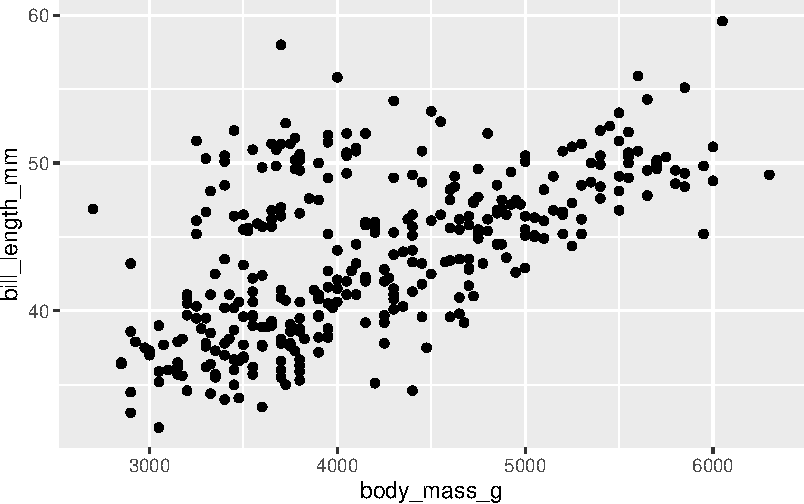
\includegraphics{03-Visualization_files/figure-pdf/unnamed-chunk-6-1.pdf}

}

\caption{Relation entre masse corporelle et longueur du bec chez les
manchots de l'archipel de Palmer}

\end{figure}%

Au moment de produire ce graphique, \texttt{R} nous indique que 2 lignes
du tableau \texttt{penguins} ne figurent pas sur ce graphique car elles
possèdent des données manquantes (\texttt{NA}), pour l'une et/ou l'autre
des variables que nous avons sélectionnées. La fonction
\texttt{geom\_point()} est donc incapable de les placer sur le
graphique.

Vous avez donc ici un premier exemple de graphique très simple. Il est
loin d'être parfait (à minima, le titre des axes devrait être modifié),
mais il a le mérite de vous présenter la syntaxe que vous devrez
utiliser pour produire presque tous les graphiques qui vous seront
utiles avec \texttt{ggplot2}. En outre, on peut percevoir qu'il semble
exister une relation positive (mais imparfaite) entre longueur des becs
et masse des individus. Il faut toutefois être prudent car nous avons
ici utilisé toutes les données disponibles (donc les données des 3
espèces à la fois), ce qui est loin d'être pertinent.

\begin{tcolorbox}[enhanced jigsaw, colbacktitle=quarto-callout-tip-color!10!white, colframe=quarto-callout-tip-color-frame, bottomtitle=1mm, opacityback=0, arc=.35mm, leftrule=.75mm, titlerule=0mm, colback=white, title=\textcolor{quarto-callout-tip-color}{\faLightbulb}\hspace{0.5em}{En résumé}, toptitle=1mm, breakable, coltitle=black, rightrule=.15mm, left=2mm, opacitybacktitle=0.6, toprule=.15mm, bottomrule=.15mm]

\begin{itemize}
\tightlist
\item
  Au sein de la fonction \texttt{ggplot()}, on spécifie 2 composants de
  la grammaire des graphiques :

  \begin{enumerate}
  \def\labelenumi{\arabic{enumi}.}
  \tightlist
  \item
    le nom du tableau contenant les données grâce à l'argument
    \texttt{data\ =\ penguins}
  \item
    l'association (\texttt{mapping}) des variables du tableau de données
    à des caractéristiques esthétiques (\texttt{aes()}) en précisant
    \texttt{aes(x\ =\ body\_mass\_g,\ y\ =\ bill\_length\_mm)} :

    \begin{itemize}
    \tightlist
    \item
      la variable \texttt{body\_mass\_g} est associée à l'esthétique de
      position \texttt{x}
    \item
      la variable \texttt{bill\_length\_mm} est associée à l'esthétique
      de position \texttt{y}
    \end{itemize}
  \end{enumerate}
\item
  On ajoute une couche au graphique \texttt{ggplot()} grâce au symbole
  \texttt{+}. La couche en question précise le troisième élément
  indispensable de la grammaire des graphiques : l'objet
  \texttt{geom}étrique. Ici, les objets sont des \texttt{point}s. On le
  spécifie grâce à la fonction \texttt{geom\_point()}.
\end{itemize}

\end{tcolorbox}

Quelques remarques concernant les couches :

\begin{itemize}
\tightlist
\item
  Notez que le signe \texttt{+} est placé \emph{à la fin de la ligne}.
  Vous recevrez un message d'erreur si vous le placez au début.
\item
  Quand vous ajoutez une couche à un graphique, je vous encourage
  vivement à presser la touche \texttt{enter} de votre clavier juste
  après le symbole \texttt{+}. Ainsi, le code correspondant à chaque
  couche sera sur une ligne distincte, ce qui augmente considérablement
  la lisibilité de votre code.
\item
  Comme indiqué dans la Section~\ref{sec-functions}, tant que les
  arguments d'une fonction sont spécifiés dans l'ordre, on peut se
  passer d'écrire leur nom. Ainsi, les deux blocs de commande suivants
  produisent exactement le même résultat :
\end{itemize}

\begin{Shaded}
\begin{Highlighting}[]
\CommentTok{\# Le nom des arguments est précisé}
\FunctionTok{ggplot}\NormalTok{(}\AttributeTok{data =}\NormalTok{ penguins, }\AttributeTok{mapping =} \FunctionTok{aes}\NormalTok{(}\AttributeTok{x =}\NormalTok{ body\_mass\_g, }\AttributeTok{y =}\NormalTok{ bill\_length\_mm)) }\SpecialCharTok{+}
  \FunctionTok{geom\_point}\NormalTok{()}

\CommentTok{\# Le nom des arguments est omis}
\FunctionTok{ggplot}\NormalTok{(penguins, }\FunctionTok{aes}\NormalTok{(}\AttributeTok{x =}\NormalTok{ body\_mass\_g, }\AttributeTok{y =}\NormalTok{ bill\_length\_mm)) }\SpecialCharTok{+}
  \FunctionTok{geom\_point}\NormalTok{()}
\end{Highlighting}
\end{Shaded}

\subsection{Exercices}\label{sec-exo-3}

\begin{enumerate}
\def\labelenumi{\arabic{enumi}.}
\tightlist
\item
  Donnez une raison pratique expliquant pourquoi les variables
  \texttt{body\_mass\_g} et \texttt{bill\_length\_mm} ont une relation
  positive
\item
  Quelles variables (pas nécessairement dans le tableau
  \texttt{penguins}) pourraient avoir une corrélation négative (relation
  négative) avec \texttt{body\_mass\_g} ? Pourquoi ? Rappelez-vous que
  nous étudions ici des variables numériques.
\item
  Citez les éléments de ce graphique/de ces données qui vous sautent le
  plus aux yeux ?
\item
  Créez un nouveau nuage de points en utilisant d'autres variables du
  jeu de données \texttt{penguins}
\end{enumerate}

\section{Quel graphique dans quelle situation
?}\label{quel-graphique-dans-quelle-situation}

Il n'est pas possible de faire n'importe quel type de graphique dans
n'importe quelle situation. Selon le nombre de variables dont on dispose
ou que l'on souhaite examiner, et selon la nature de ces variables
(numériques et/ou catégorielles), le choix des types de graphiques
possibles sera limité. Par exemple, les diagrammes bâtons sont réservés
aux variables catégorielles, alors que les histogrammes sont possibles
uniquement avec les variables numériques continues. Néanmoins, dans
certaines situations, plusieurs choix de graphiques seront possibles, et
vous aurez donc une certaine liberté. Vos choix seront alors guidés par
les objectifs que vous souhaiterez atteindre grâce aux graphiques, ainsi
que par vos préférences.

\begin{tcolorbox}[enhanced jigsaw, colbacktitle=quarto-callout-note-color!10!white, colframe=quarto-callout-note-color-frame, bottomtitle=1mm, opacityback=0, arc=.35mm, leftrule=.75mm, titlerule=0mm, colback=white, title=\textcolor{quarto-callout-note-color}{\faInfo}\hspace{0.5em}{Objectifs}, toptitle=1mm, breakable, coltitle=black, rightrule=.15mm, left=2mm, opacitybacktitle=0.6, toprule=.15mm, bottomrule=.15mm]

Dans la suite de ce chapitre, nous traiterons donc des situations les
plus courantes : quel(s) type(s) de graphique(s) produire lorsque l'on
dispose d'une, deux ou trois variables ? Quel(s) type(s) de graphique(s)
produire lorsque les variables sont toutes numériques, toutes
catégorielles, ou lorsqu'on dispose de variables des deux types ?

Pour chaque situation, un ou des exemples seront fournis à partir des
données du tableau \texttt{penguins}. Cela sera aussi l'occasion de
présenter quelques-unes des nombreuses subtilités liées à l'utilisation
du package \texttt{ggplot2}.

\end{tcolorbox}

\section{Une seule variable
numérique}\label{une-seule-variable-numuxe9rique}

Lorsque l'on souhaite examiner une unique variable numérique, deux types
de représentations graphiques sont en général possibles :

\begin{enumerate}
\def\labelenumi{\arabic{enumi}.}
\tightlist
\item
  les histogrammes : la variable d'intérêt est placée sur l'axe des
  \texttt{x} du graphique. Les valeurs utilisées sur l'axe des
  \texttt{y} est calculée automatiquement par le logiciel.
\item
  les nuages de points : la variable d'intérêt est placée sur l'axe des
  \texttt{y}. L'axe des \texttt{x} porte soit un simple numéro d'indice
  pour chaque observation, soit une unique valeur sans importance, la
  même pour toutes les observations.
\end{enumerate}

Les syntaxes et options pour ces 2 types de graphiques sont présentées
ci-dessous.

\subsection{Les histogrammes}\label{sec-histo}

\subsubsection{Syntaxe élémentaire}\label{syntaxe-uxe9luxe9mentaire}

Imaginons que l'on s'intéresse à la variable \texttt{body\_mass\_g} du
jeu de données \texttt{penguins}.

La syntaxe permettant de produire un histogramme, sous sa forme la plus
simple, est la suivante :

\begin{Shaded}
\begin{Highlighting}[]
\FunctionTok{ggplot}\NormalTok{(penguins, }\FunctionTok{aes}\NormalTok{(}\AttributeTok{x =}\NormalTok{ body\_mass\_g)) }\SpecialCharTok{+}
  \FunctionTok{geom\_histogram}\NormalTok{()}
\end{Highlighting}
\end{Shaded}

\begin{verbatim}
`stat_bin()` using `bins = 30`. Pick better value with `binwidth`.
\end{verbatim}

\begin{verbatim}
Warning: Removed 2 rows containing non-finite outside the scale range
(`stat_bin()`).
\end{verbatim}

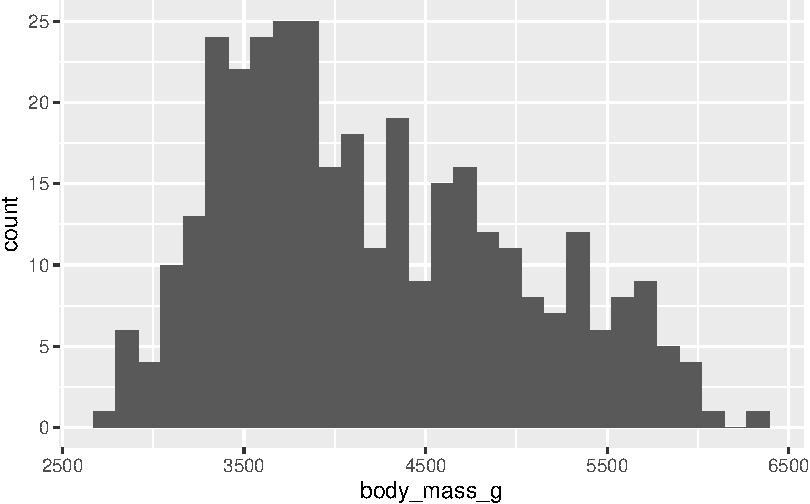
\includegraphics{03-Visualization_files/figure-pdf/unnamed-chunk-8-1.pdf}

Deux messages nous sont adressés par le logiciel :

\begin{enumerate}
\def\labelenumi{\arabic{enumi}.}
\tightlist
\item
  \texttt{Warning:\ Removed\ 2\ rows\ containing\ non-finite\ values\ (stat\_bin)}.
  Ce message indique, comme pour le premier nuage de points, que 2
  individus du tableau \texttt{penguins} ont une masse corporelle
  inconnue (\texttt{NA}). Ces 2 individus (donc les deux lignes
  correspondantes), ont été ignorés pour produire ce graphique
\item
  \texttt{\textquotesingle{}stat\_bin()\textquotesingle{}\ using\ \textquotesingle{}bins\ =\ 30\textquotesingle{}.\ Pick\ better\ value\ with\ \textquotesingle{}binwidth\textquotesingle{}}.
  Ce message indique que \texttt{R} a choisi pour nous les limites des
  classes utilisées pour faire l'histogramme. Sur un histogramme, la
  variable d'intérêt (toujours numérique et continue), qui apparaît sur
  l'axe des abscisses, est en effet ``découpée'' en plusieurs classes,
  en général de même taille, afin de permettre une représentation de la
  \textbf{distribution des valeurs}. Ici, \texttt{R} indique qu'il a
  créé 30 catégories pour nous, et que nous pouvons faire un choix
  différent grâce à l'argument \texttt{binwidth}. Nous y reviendrons un
  peu plus loin.
\end{enumerate}

Sur ce graphique, l'axe des abscisses porte donc la variable continue
``découpée'' en classes de mêmes largeur, et l'axe des ordonnées
renseigne sur le nombre (\texttt{count} ou fréquence absolue)
d'individus observés dans chaque classe. Les zones du graphique où les
barres sont les plus hautes indiquent donc les caractéristiques des
individus observés le plus fréquemment. À l'inverse, les barres les plus
courtes correspondent à des valeurs de masse rarement observées. Au
final, ce type de graphique permet de visualiser \textbf{la distribution
des données pour une variable numérique continue}.

Ici, on constate qu'une majorité d'individus semble avoir des masses
proches de 3500 grammes. Une autre portion non négligeable des individus
(mais moins importante) semble avoir une masse légèrement supérieure à
4500 grammes. Enfin, les masses supérieures à 6000 grammes sont très
rares. L'histogramme nous permet également de visualiser l'étendue des
données : les manchots étudiés ici ont des masses qui s'étalent d'un peu
plus de 2500 grammes à un peu moins de 6500 grammes.

\subsubsection{Couleur}\label{couleur}

Pour rendre ce graphique plus facilement lisible, on peut en modifier la
couleur :

\begin{itemize}
\tightlist
\item
  la couleur de remplissage des barres peut-être spécifiée grâce à
  l'argument \texttt{fill\ =}
\item
  la couleur de contour des barres peut-être spécifiée grâce à
  l'argument \texttt{color\ =}
\end{itemize}

Une liste des couleurs disponibles dans \texttt{R} peut être affichée
dans la console en tapant :

\begin{Shaded}
\begin{Highlighting}[]
\FunctionTok{colors}\NormalTok{()}
\end{Highlighting}
\end{Shaded}

Vous pouvez voir à quelle couleur correspond chacun de ces noms
\href{http://www.stat.columbia.edu/~tzheng/files/Rcolor.pdf}{dans ce
document pdf}.

Mettons à jour notre histogramme en ajoutant un peu de couleur :

\begin{Shaded}
\begin{Highlighting}[]
\FunctionTok{ggplot}\NormalTok{(penguins, }\FunctionTok{aes}\NormalTok{(}\AttributeTok{x =}\NormalTok{ body\_mass\_g)) }\SpecialCharTok{+}
  \FunctionTok{geom\_histogram}\NormalTok{(}\AttributeTok{fill =} \StringTok{"steelblue"}\NormalTok{, }\AttributeTok{color =} \StringTok{"black"}\NormalTok{)}
\end{Highlighting}
\end{Shaded}

\begin{verbatim}
`stat_bin()` using `bins = 30`. Pick better value with `binwidth`.
\end{verbatim}

\begin{verbatim}
Warning: Removed 2 rows containing non-finite outside the scale range
(`stat_bin()`).
\end{verbatim}

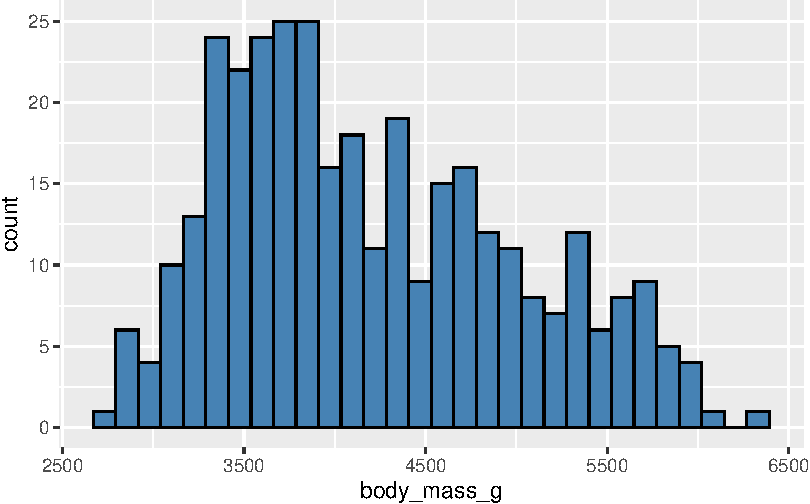
\includegraphics{03-Visualization_files/figure-pdf/unnamed-chunk-10-1.pdf}

Les 30 classes de masses sont maintenant plus facilement visibles et
distingables.

\subsubsection{\texorpdfstring{À l'intérieur ou à l'extérieur de
\texttt{aes()}
?}{À l'intérieur ou à l'extérieur de aes() ?}}\label{uxe0-lintuxe9rieur-ou-uxe0-lextuxe9rieur-de-aes}

Les couleurs de remplissage et de contour des barres d'un histogramme
font partie des caractéristiques esthétiques du graphique. Pourtant,
elles ne sont pas précisées à l'intérieur de la fonction \texttt{aes()}.
La raison est simple mais importante :

\begin{tcolorbox}[enhanced jigsaw, colbacktitle=quarto-callout-important-color!10!white, colframe=quarto-callout-important-color-frame, bottomtitle=1mm, opacityback=0, arc=.35mm, leftrule=.75mm, titlerule=0mm, colback=white, title=\textcolor{quarto-callout-important-color}{\faExclamation}\hspace{0.5em}{Important}, toptitle=1mm, breakable, coltitle=black, rightrule=.15mm, left=2mm, opacitybacktitle=0.6, toprule=.15mm, bottomrule=.15mm]

On place à l'intérieur de \texttt{aes()} uniquement les caractéristiques
esthétiques du graphique que l'on souhaite associer à des
\textbf{variables du jeu de données}.

\end{tcolorbox}

Ici, les couleurs que l'on indique sont des constantes : toutes les
barres ont les mêmes couleur de remplissage et de contour. On n'associe
pas une variable du jeu de données à ces caractéristiques esthétiques.
On place donc \texttt{fill\ =} et \texttt{color\ =} à l'extérieur de
\texttt{aes()}. Si on se trompe, voilà ce qui se produit :

\begin{Shaded}
\begin{Highlighting}[]
\FunctionTok{ggplot}\NormalTok{(penguins, }\FunctionTok{aes}\NormalTok{(}\AttributeTok{x =}\NormalTok{ body\_mass\_g)) }\SpecialCharTok{+}
  \FunctionTok{geom\_histogram}\NormalTok{(}\FunctionTok{aes}\NormalTok{(}\AttributeTok{fill =} \StringTok{"steelblue"}\NormalTok{, }\AttributeTok{color =} \StringTok{"black"}\NormalTok{))}
\end{Highlighting}
\end{Shaded}

\begin{verbatim}
`stat_bin()` using `bins = 30`. Pick better value with `binwidth`.
\end{verbatim}

\begin{verbatim}
Warning: Removed 2 rows containing non-finite outside the scale range
(`stat_bin()`).
\end{verbatim}

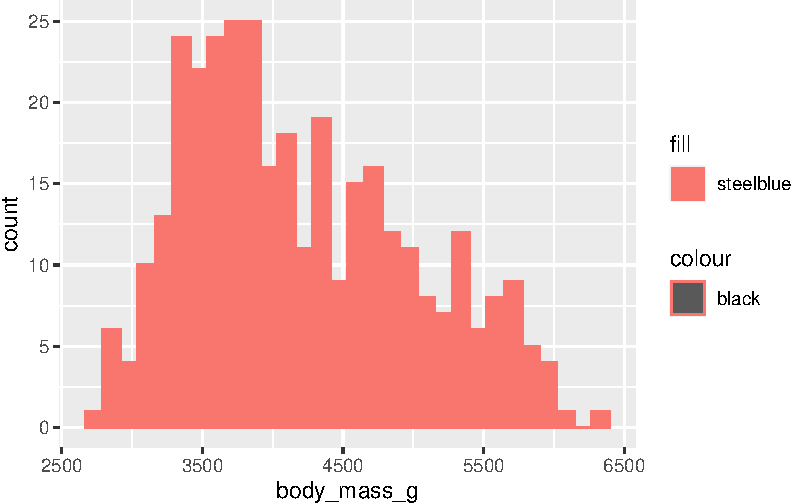
\includegraphics{03-Visualization_files/figure-pdf/unnamed-chunk-11-1.pdf}

Les couleurs qui apparaissent ne correspondent pas à ce qui est demandé,
et une légende ne correspondant à rien apparaît à droite du graphique.
La syntaxe utilisée ici suppose en effet que \texttt{"steelblue"} et
\texttt{"black"} seraient des variables du jeu de données
\texttt{penguins}. Puisqu'elles n'existent pas, \texttt{R} essaie de se
débrouiller pour interpréter comme il peut ce qu'on lui demande, et
finit par produire ce graphique incohérent. La couleur utilisée est la
première couleur de la palette par défaut de \texttt{ggplot2}.

Pour élaborer des graphiques plus avancés, il faudra donc toujours vous
poser la question suivante : la caractéristique esthétique que je
souhaite modifier doit-elle être associée à une \textbf{valeur
constante} que je fixe pour toutes les barres ou tous les points d'un
graphique, et alors, je l'indique \textbf{en dehors} de \texttt{aes()},
ou est-elle au contraire associée à \textbf{une variable du jeu de
données}, et alors, je l'indique \textbf{à l'intérieur} de
\texttt{aes()}.

Il est bien sûr possible d'avoir un mélange des deux. Par exemple, le
code suivant permet d'associer la couleur de remplissage au sexe des
individus étudiés (variable \texttt{sex} du jeu de données
\texttt{penguins}), et de spécifier une valeur constante pour la couleur
de contour des barres (ici, le noir) :

\begin{Shaded}
\begin{Highlighting}[]
\FunctionTok{ggplot}\NormalTok{(penguins, }\FunctionTok{aes}\NormalTok{(}\AttributeTok{x =}\NormalTok{ body\_mass\_g)) }\SpecialCharTok{+}
  \FunctionTok{geom\_histogram}\NormalTok{(}\FunctionTok{aes}\NormalTok{(}\AttributeTok{fill =}\NormalTok{ sex), }\AttributeTok{color =} \StringTok{"black"}\NormalTok{)}
\end{Highlighting}
\end{Shaded}

\begin{verbatim}
`stat_bin()` using `bins = 30`. Pick better value with `binwidth`.
\end{verbatim}

\begin{verbatim}
Warning: Removed 2 rows containing non-finite outside the scale range
(`stat_bin()`).
\end{verbatim}

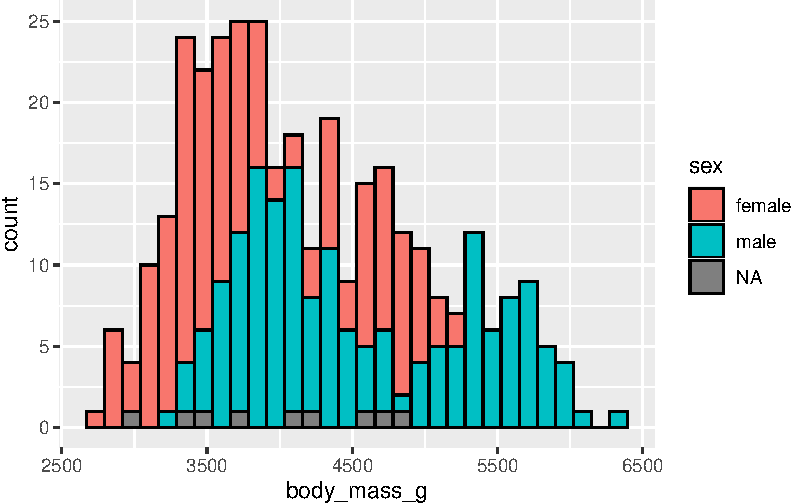
\includegraphics{03-Visualization_files/figure-pdf/unnamed-chunk-12-1.pdf}

On constate que toutes les barres ont un contour noir, mais que
plusieurs couleurs de remplissage apparaissent maintenant, selon le sexe
des individus, dans chaque classe de masse. Une légende adaptée est
aussi créée automatiquement à droite du graphique. On apprend ainsi que
les individus les plus lourds sont tous des mâles. On constate également
que le sexe de certains individus est inconnu.

Au final, nous ne sommes déjà plus dans la situation où on examine une
unique variable numérique. Nous avons en effet ici un graphique nous
permettant de mettre en relation une variable numérique (la masse des
individus en grammes) et une variable catégorielle (le sexe des
individus). Nous reviendrons plus tard sur ce type de graphiques.

\subsubsection{La largeur des classes}\label{la-largeur-des-classes}

Comme évoqué plus haut, par défaut, \texttt{R} choisit arbitrairement de
découper la variable numérique utilisée en 30 classes de même largeur
afin de produire l'histogramme. Ça n'est que rarement un bon choix, et
malheureusement, il n'y a pas de règle permettant de définir à coup sûr
le bon nombre de classes pour visualiser au mieux la distribution d'une
variable numérique. Il faut en effet presque toujours procéder par
essais-erreurs successifs. Il est possible d'ajuster les
caractéristiques (nombre et/ou largeur) des classes de l'histogramme de
l'une des 3 façons suivantes :

\begin{enumerate}
\def\labelenumi{\arabic{enumi}.}
\tightlist
\item
  En ajustant le nombre de classes avec \texttt{bins}.
\item
  En précisant la largeur des classes avec \texttt{binwidth}.
\item
  En fournissant manuellement les limites des classes avec
  \texttt{breaks}.
\end{enumerate}

\begin{Shaded}
\begin{Highlighting}[]
\FunctionTok{ggplot}\NormalTok{(penguins, }\FunctionTok{aes}\NormalTok{(}\AttributeTok{x =}\NormalTok{ body\_mass\_g)) }\SpecialCharTok{+}
  \FunctionTok{geom\_histogram}\NormalTok{(}\AttributeTok{fill =} \StringTok{"steelblue"}\NormalTok{, }\AttributeTok{color =} \StringTok{"black"}\NormalTok{,}
                 \AttributeTok{bins =} \DecValTok{10}\NormalTok{)}
\end{Highlighting}
\end{Shaded}

\begin{verbatim}
Warning: Removed 2 rows containing non-finite outside the scale range
(`stat_bin()`).
\end{verbatim}

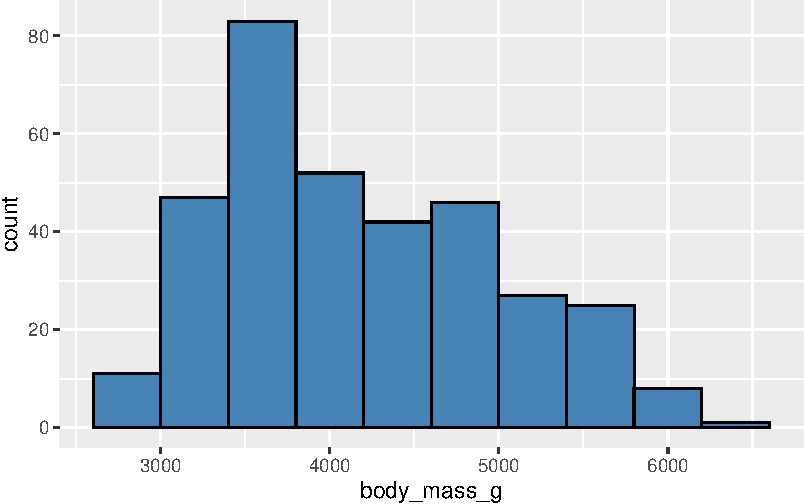
\includegraphics{03-Visualization_files/figure-pdf/unnamed-chunk-13-1.pdf}

Ici, diminuer le nombre de classes à 10 a pour effet de trop lisser la
distribution des données. On ne visualise plus les variations subtiles
de la distribution. À l'inverse, trop augmenter le nombre de classes
n'est pas pertinent non plus :

\begin{Shaded}
\begin{Highlighting}[]
\FunctionTok{ggplot}\NormalTok{(penguins, }\FunctionTok{aes}\NormalTok{(}\AttributeTok{x =}\NormalTok{ body\_mass\_g)) }\SpecialCharTok{+}
  \FunctionTok{geom\_histogram}\NormalTok{(}\AttributeTok{fill =} \StringTok{"steelblue"}\NormalTok{, }\AttributeTok{color =} \StringTok{"black"}\NormalTok{,}
                 \AttributeTok{bins =} \DecValTok{100}\NormalTok{)}
\end{Highlighting}
\end{Shaded}

\begin{verbatim}
Warning: Removed 2 rows containing non-finite outside the scale range
(`stat_bin()`).
\end{verbatim}

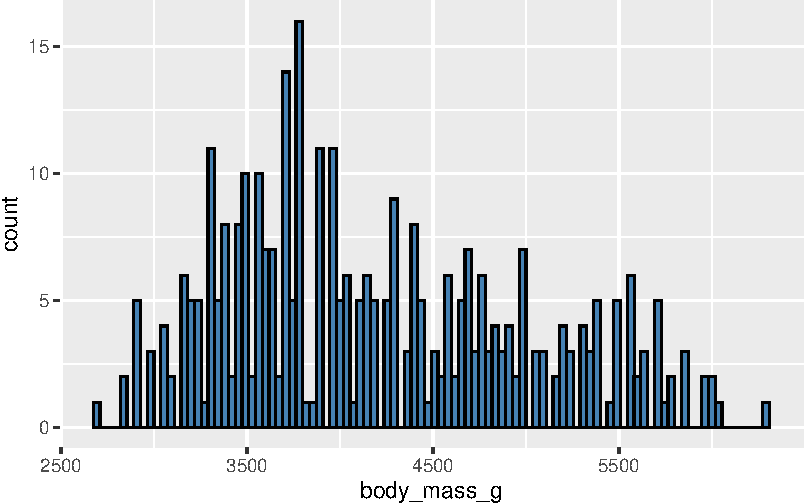
\includegraphics{03-Visualization_files/figure-pdf/unnamed-chunk-14-1.pdf}

Ici, passer à 100 classes de taille génère un histogramme plein de
trous, avec des classes très étroites, dont certaines sont très
représentées, et immédiatement suivies ou précédées par des classes très
peu représentées. Cela n'a pas de logique, et c'est presque toujours le
signe qu'il faut réduire le nombre de classes.

Au final, pour ces données, un nombre de classes compris entre 20 et 30
semble un bon choix :

\begin{Shaded}
\begin{Highlighting}[]
\FunctionTok{ggplot}\NormalTok{(penguins, }\FunctionTok{aes}\NormalTok{(}\AttributeTok{x =}\NormalTok{ body\_mass\_g)) }\SpecialCharTok{+}
  \FunctionTok{geom\_histogram}\NormalTok{(}\AttributeTok{fill =} \StringTok{"steelblue"}\NormalTok{, }\AttributeTok{color =} \StringTok{"black"}\NormalTok{,}
                 \AttributeTok{bins =} \DecValTok{25}\NormalTok{)}
\end{Highlighting}
\end{Shaded}

\begin{verbatim}
Warning: Removed 2 rows containing non-finite outside the scale range
(`stat_bin()`).
\end{verbatim}

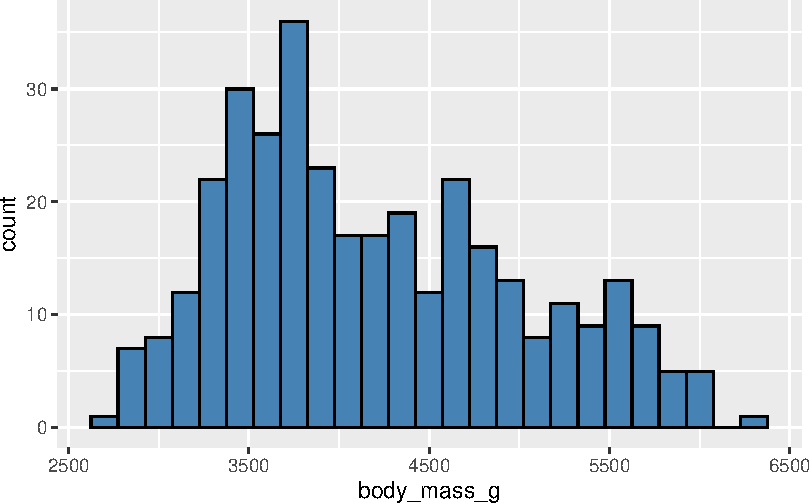
\includegraphics{03-Visualization_files/figure-pdf/unnamed-chunk-15-1.pdf}

C'est un bon choix, entre trop peu d'information, et trop de bruit
visuel. Évidemment, ce nombre sera différent pour chaque jeu de données.
On constate ici à peu près 3 pics (autour de 3500 grammes, un peu
au-dessus de 4500 grammes, et autour de 5500 grammes) qui reflètent bien
la distribution de ces données.

On peut également modifier \textbf{la largeur des classes} (et non plus
leur nombre) avec \texttt{binwidth} :

\begin{Shaded}
\begin{Highlighting}[]
\FunctionTok{ggplot}\NormalTok{(penguins, }\FunctionTok{aes}\NormalTok{(}\AttributeTok{x =}\NormalTok{ body\_mass\_g)) }\SpecialCharTok{+}
  \FunctionTok{geom\_histogram}\NormalTok{(}\AttributeTok{fill =} \StringTok{"steelblue"}\NormalTok{, }\AttributeTok{color =} \StringTok{"black"}\NormalTok{,}
                 \AttributeTok{binwidth =} \DecValTok{200}\NormalTok{)}
\end{Highlighting}
\end{Shaded}

\begin{verbatim}
Warning: Removed 2 rows containing non-finite outside the scale range
(`stat_bin()`).
\end{verbatim}

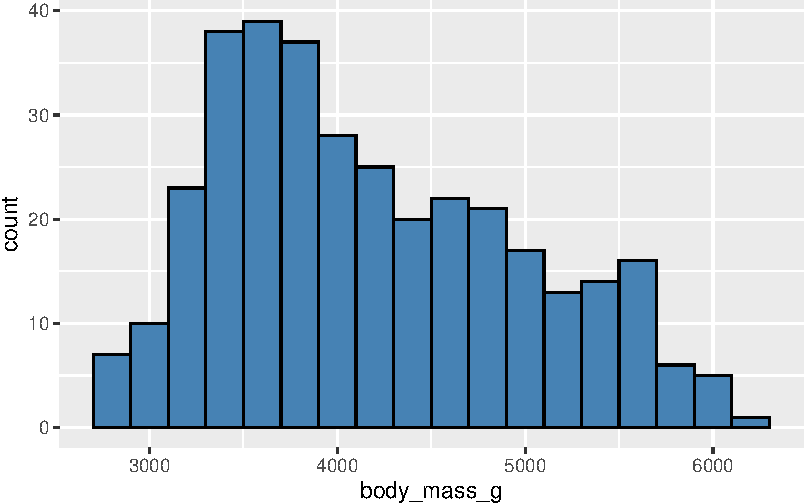
\includegraphics{03-Visualization_files/figure-pdf/unnamed-chunk-16-1.pdf}

Ici, chaque catégorie recouvre 200 grammes. Avec l'argument
\texttt{bins}, on indique à \texttt{R} combien on souhaite obtenir de
classes, et il détermine automatiquement leur largeur. Avec
\texttt{binwidth}, on indique la largeur des classes souhaitées, et
\texttt{R} détermine automatiquement le nombre de classes nécessaires
pour couvrir la totalité des données.

Enfin, il est possible de déterminer manuellement les limites des
classes souhaitées avec l'argument \texttt{breaks} :

\begin{Shaded}
\begin{Highlighting}[]
\FunctionTok{ggplot}\NormalTok{(penguins, }\FunctionTok{aes}\NormalTok{(}\AttributeTok{x =}\NormalTok{ body\_mass\_g)) }\SpecialCharTok{+}
  \FunctionTok{geom\_histogram}\NormalTok{(}\AttributeTok{fill =} \StringTok{"steelblue"}\NormalTok{, }\AttributeTok{color =} \StringTok{"black"}\NormalTok{,}
                 \AttributeTok{breaks =} \FunctionTok{c}\NormalTok{(}\DecValTok{2500}\NormalTok{, }\DecValTok{2750}\NormalTok{, }\DecValTok{3000}\NormalTok{, }\DecValTok{3500}\NormalTok{, }\DecValTok{4000}\NormalTok{, }\DecValTok{4500}\NormalTok{, }\DecValTok{5000}\NormalTok{, }\DecValTok{6000}\NormalTok{, }\DecValTok{7000}\NormalTok{))}
\end{Highlighting}
\end{Shaded}

\begin{verbatim}
Warning: Removed 2 rows containing non-finite outside the scale range
(`stat_bin()`).
\end{verbatim}

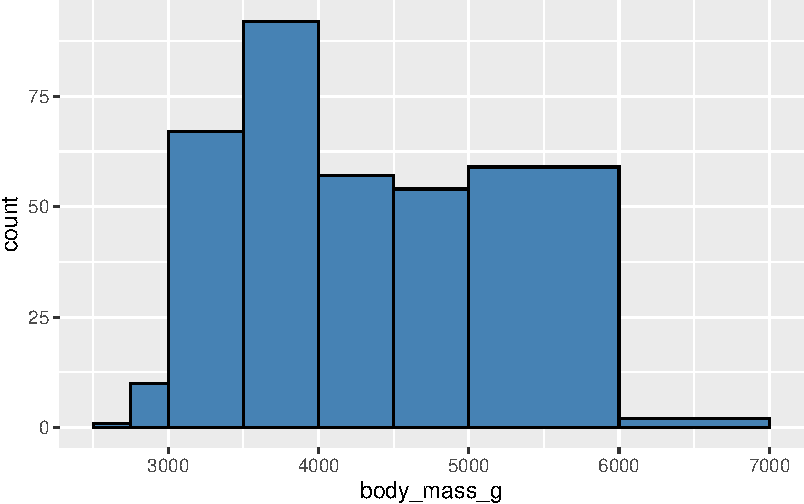
\includegraphics{03-Visualization_files/figure-pdf/unnamed-chunk-17-1.pdf}

Vous constatez ici que les choix effectués ne sont pas très pertinents :
toutes les classes n'ont pas la même largeur. Cela rend l'interprétation
difficile. Il est donc vivement conseillé, pour spécifier
\texttt{breaks}, de créer des suites régulières, comme avec la fonction
\texttt{seq()} (consultez son fichier d'aide et les exemples) :

\begin{Shaded}
\begin{Highlighting}[]
\NormalTok{limites }\OtherTok{\textless{}{-}} \FunctionTok{seq}\NormalTok{(}\AttributeTok{from =} \DecValTok{2500}\NormalTok{, }\AttributeTok{to =} \DecValTok{6500}\NormalTok{, }\AttributeTok{by =} \DecValTok{250}\NormalTok{)}
\NormalTok{limites}
\end{Highlighting}
\end{Shaded}

\begin{verbatim}
 [1] 2500 2750 3000 3250 3500 3750 4000 4250 4500 4750 5000 5250 5500 5750 6000
[16] 6250 6500
\end{verbatim}

\begin{Shaded}
\begin{Highlighting}[]
\FunctionTok{ggplot}\NormalTok{(penguins, }\FunctionTok{aes}\NormalTok{(}\AttributeTok{x =}\NormalTok{ body\_mass\_g)) }\SpecialCharTok{+}
  \FunctionTok{geom\_histogram}\NormalTok{(}\AttributeTok{fill =} \StringTok{"steelblue"}\NormalTok{, }\AttributeTok{color =} \StringTok{"black"}\NormalTok{,}
                 \AttributeTok{breaks =}\NormalTok{ limites)}
\end{Highlighting}
\end{Shaded}

\begin{figure}[H]

{\centering 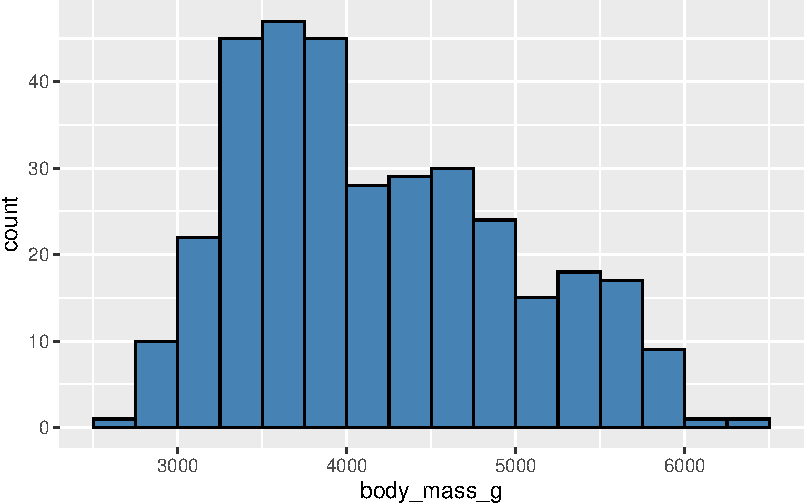
\includegraphics{03-Visualization_files/figure-pdf/unnamed-chunk-18-1.pdf}

}

\caption{Un exemple d'utilisation de l'argument \texttt{breaks}}

\end{figure}%

Il est important que toute la gamme des valeurs de
\texttt{body\_mass\_g} soit bien couverte par les limites des classes
que nous avons définies, sinon, certaines valeurs sont omises et
l'histogramme est donc incomplet/incorrect. Une façon de s'en assurer
est d'afficher le résumé des données pour la colonne
\texttt{body\_mass\_g} du jeu de données \texttt{penguins} :

\begin{Shaded}
\begin{Highlighting}[]
\FunctionTok{summary}\NormalTok{(penguins}\SpecialCharTok{$}\NormalTok{body\_mass\_g)}
\end{Highlighting}
\end{Shaded}

\begin{verbatim}
   Min. 1st Qu.  Median    Mean 3rd Qu.    Max.    NA's 
   2700    3550    4050    4202    4750    6300       2 
\end{verbatim}

On voit ici que les masses varient de 2700 à 6300 grammes. Les classes
que nous avons définies couvrent une plage de masses plus large (de 2500
à 6500). Toutes les données sont donc bien intégrées à l'histogramme.

\subsubsection{\texorpdfstring{\texttt{geom\_rug} et
\texttt{geom\_density}}{geom\_rug et geom\_density}}\label{sec-density}

La fonction \texttt{geom\_histogram()} n'est pas la seule qui permette
de visualiser la distribution des données. Il est en effet possible
d'utiliser d'autres objets géométriques, en plus ou à la place de
\texttt{geom\_histogram()} pour ajouter de l'information sur le
graphique, ou pour visualiser différemment la distribution des mêmes
données.

La fonction \texttt{geom\_rug()} permet d'ajouter les données réelles
sous forme de segments, sous un histogramme. Cela prend souvent l'aspect
d'une sorte de tapis, d'où le nom de la fonction (``rug'' signifie
``tapis'' en anglais). Pour ajouter une couche supplémentaire au
graphique, on ajoute simplement un \texttt{+} à la fin de la dernière
ligne, et sur la ligne suivante, on ajoute un objet géométrique
supplémentaire :

\begin{Shaded}
\begin{Highlighting}[]
\FunctionTok{ggplot}\NormalTok{(penguins, }\FunctionTok{aes}\NormalTok{(}\AttributeTok{x =}\NormalTok{ body\_mass\_g)) }\SpecialCharTok{+}
  \FunctionTok{geom\_histogram}\NormalTok{(}\AttributeTok{fill =} \StringTok{"steelblue"}\NormalTok{, }\AttributeTok{color =} \StringTok{"black"}\NormalTok{,}
                 \AttributeTok{bins =} \DecValTok{25}\NormalTok{) }\SpecialCharTok{+}
  \FunctionTok{geom\_rug}\NormalTok{()}
\end{Highlighting}
\end{Shaded}

\begin{verbatim}
Warning: Removed 2 rows containing non-finite outside the scale range
(`stat_bin()`).
\end{verbatim}

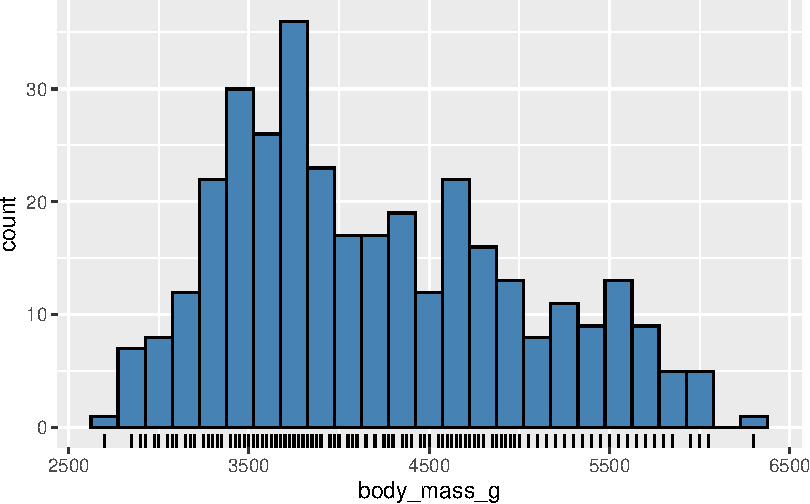
\includegraphics{03-Visualization_files/figure-pdf/unnamed-chunk-20-1.pdf}

Les tirets qui sont maintenant visibles en-dessous de l'histogramme
correspondent aux 342 valeurs de masses réellement observées dans le jeu
de données. Puisque certaines tailles ont été observées plusieurs fois,
faire des tirets semi-transparents nous permettra de mieux visualiser
quelles tailles ont été observées fréquemment ou rarement. On peut
régler la transparence des éléments d'un graphique avec l'argument
\texttt{alpha\ =}, qui prend des valeurs comprises entre 0 (transparence
totale) et 1 (opacité totale) :

\begin{Shaded}
\begin{Highlighting}[]
\FunctionTok{ggplot}\NormalTok{(penguins, }\FunctionTok{aes}\NormalTok{(}\AttributeTok{x =}\NormalTok{ body\_mass\_g)) }\SpecialCharTok{+}
  \FunctionTok{geom\_histogram}\NormalTok{(}\AttributeTok{fill =} \StringTok{"steelblue"}\NormalTok{, }\AttributeTok{color =} \StringTok{"black"}\NormalTok{,}
                 \AttributeTok{bins =} \DecValTok{25}\NormalTok{) }\SpecialCharTok{+}
  \FunctionTok{geom\_rug}\NormalTok{(}\AttributeTok{alpha =} \FloatTok{0.3}\NormalTok{)}
\end{Highlighting}
\end{Shaded}

\begin{verbatim}
Warning: Removed 2 rows containing non-finite outside the scale range
(`stat_bin()`).
\end{verbatim}

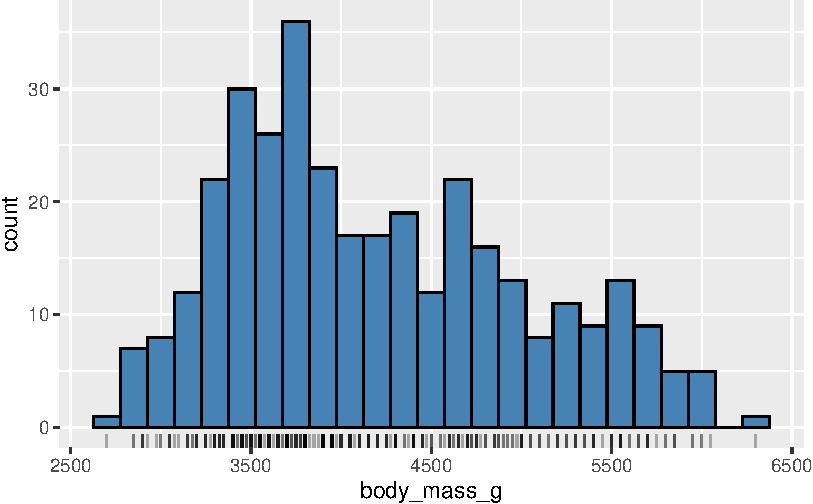
\includegraphics{03-Visualization_files/figure-pdf/unnamed-chunk-21-1.pdf}

Les tirets sont maintenant d'autant plus foncés que les tailles ont été
observées un grand nombre de fois. On retrouve bien ici la distribution
décrite plus haut, avec 3 principaux groupes de valeurs. Cela révèle
certainement en partie la complexité des données : ces tailles
correspondent en effet aux mesures effectuées chez 3 espèces distinctes
qui peuvent avoir des caractéristiques différentes, sans compter que le
sexe des individus, qui n'apparaît pas ici, entre aussi probablement en
jeu. Nous y reviendrons plus tard.

La fonction \texttt{geom\_density()} permet de s'affranchir de la
question du nombre ou de la largeur des classes de taille :

\begin{Shaded}
\begin{Highlighting}[]
\FunctionTok{ggplot}\NormalTok{(penguins, }\FunctionTok{aes}\NormalTok{(}\AttributeTok{x =}\NormalTok{ body\_mass\_g)) }\SpecialCharTok{+}
  \FunctionTok{geom\_density}\NormalTok{(}\AttributeTok{fill =} \StringTok{"steelblue"}\NormalTok{, }\AttributeTok{color =} \StringTok{"black"}\NormalTok{, }\AttributeTok{alpha =} \FloatTok{0.7}\NormalTok{, }\AttributeTok{bw =} \DecValTok{300}\NormalTok{)}
\end{Highlighting}
\end{Shaded}

\begin{verbatim}
Warning: Removed 2 rows containing non-finite outside the scale range
(`stat_density()`).
\end{verbatim}

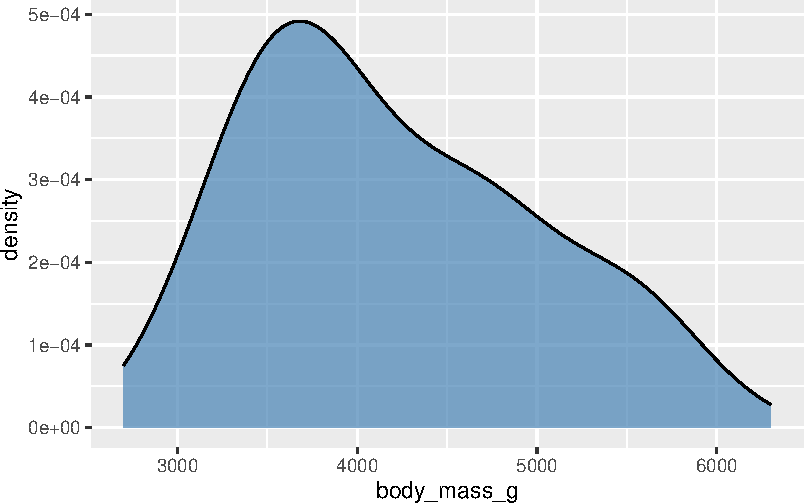
\includegraphics{03-Visualization_files/figure-pdf/unnamed-chunk-22-1.pdf}

On obtient une sorte d'histogramme lissé qui fait bien apparaître les 3
tailles les plus fréquentes (au niveau des 3 ``bosses'' du graphique).
Inutile ici de spécifier un nombre de classes de taille, ou leur largeur
: le lissage est ici automatique. On peut modifier l'importance du
lissage avec l'argument \texttt{bw}, mais la valeur choisie par défaut
par \texttt{R} est généralement tout à fait satisfaisante. Vous pouvez
essayer avec une valeur de lissage de 30, puis de 500 pour vous rendre
compte de l'effet de ce paramètre.

Notez également que si l'histogramme présentait des valeurs d'abondance
sur l'axe des \texttt{y} (des nombres d'individus), le graphique de
densité présente, comme son nom l'indique, l'information de densité des
observations. Cela signifie que la surface totale sous la courbe (en
bleu) vaut 1. Cela peut s'avérer utile pour comparer plusieurs
distributions pour lesquelles on disposes de tailles d'échantillons très
différentes.

Enfin, on peut créer un graphique qui présentera à la fois l'histogramme
(avec \texttt{geom\_histogram()}), les données individuelles (avec
\texttt{geom\_rug()}) et la courbe de densité (avec
\texttt{geom\_density()}). Mais pour que tout s'affiche correctement, il
faut indiquer à \texttt{geom\_histogram} que l'axe des \texttt{y} doit
porter les densités et non les abondances. On fait cela en précisant
\texttt{y\ =\ after\_stat(density)}, cela indique à \texttt{R} que la
variable \texttt{density} ne figure pas dans le tableau
\texttt{penguins}, mais qu'elle est calculée par la fonction
\texttt{geom\_histogram()} :

\begin{Shaded}
\begin{Highlighting}[]
\FunctionTok{ggplot}\NormalTok{(penguins, }\FunctionTok{aes}\NormalTok{(}\AttributeTok{x =}\NormalTok{ body\_mass\_g)) }\SpecialCharTok{+}
  \FunctionTok{geom\_histogram}\NormalTok{(}\FunctionTok{aes}\NormalTok{(}\AttributeTok{y =} \FunctionTok{after\_stat}\NormalTok{(density)),}
                 \AttributeTok{fill =} \StringTok{"steelblue"}\NormalTok{, }\AttributeTok{color =} \StringTok{"black"}\NormalTok{,}
                 \AttributeTok{bins =} \DecValTok{25}\NormalTok{, }\AttributeTok{alpha =} \FloatTok{0.7}\NormalTok{) }\SpecialCharTok{+}
  \FunctionTok{geom\_rug}\NormalTok{(}\AttributeTok{alpha =} \FloatTok{0.3}\NormalTok{) }\SpecialCharTok{+}
  \FunctionTok{geom\_density}\NormalTok{(}\AttributeTok{color =} \StringTok{"purple"}\NormalTok{, }\AttributeTok{linewidth =} \DecValTok{2}\NormalTok{)}
\end{Highlighting}
\end{Shaded}

\begin{verbatim}
Warning: Removed 2 rows containing non-finite outside the scale range
(`stat_bin()`).
\end{verbatim}

\begin{verbatim}
Warning: Removed 2 rows containing non-finite outside the scale range
(`stat_density()`).
\end{verbatim}

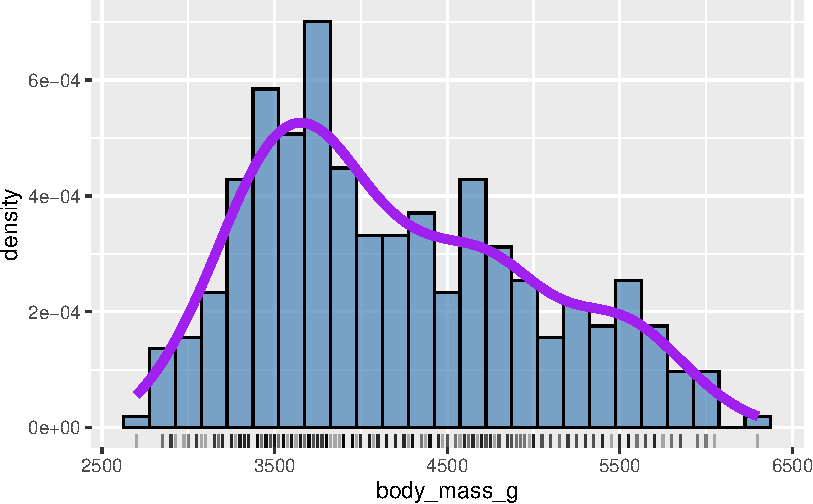
\includegraphics{03-Visualization_files/figure-pdf/unnamed-chunk-23-1.pdf}

Notez l'utilisation des arguments \texttt{alpha}, \texttt{color} et
\texttt{size}, pour modifier l'aspect de différents éléments du
graphique. Assurez-vous d'avoir compris comment on les utilise, et
faites vos propres expériences.

\subsubsection{\texorpdfstring{Un mot sur la position de la fonction
\texttt{aes()}}{Un mot sur la position de la fonction aes()}}\label{un-mot-sur-la-position-de-la-fonction-aes}

Sur le dernier exemple, vous constatez que la fonction \texttt{aes()}
apparaît une fois à l'intérieur de la fonction \texttt{ggplot()}, et une
autre fois à l'intérieur de \texttt{geom\_histogram()}. Pourquoi ne pas
avoir tapé, plus simplement :

\begin{Shaded}
\begin{Highlighting}[]
\FunctionTok{ggplot}\NormalTok{(penguins, }\FunctionTok{aes}\NormalTok{(}\AttributeTok{x =}\NormalTok{ body\_mass\_g, }\AttributeTok{y =} \FunctionTok{after\_stat}\NormalTok{(density))) }\SpecialCharTok{+}
  \FunctionTok{geom\_histogram}\NormalTok{(}\AttributeTok{fill =} \StringTok{"steelblue"}\NormalTok{, }\AttributeTok{color =} \StringTok{"black"}\NormalTok{,}
                 \AttributeTok{bins =} \DecValTok{25}\NormalTok{, }\AttributeTok{alpha =} \FloatTok{0.7}\NormalTok{) }\SpecialCharTok{+}
  \FunctionTok{geom\_rug}\NormalTok{(}\AttributeTok{alpha =} \FloatTok{0.3}\NormalTok{) }\SpecialCharTok{+}
  \FunctionTok{geom\_density}\NormalTok{(}\AttributeTok{color =} \StringTok{"purple"}\NormalTok{, }\AttributeTok{linewidth =} \DecValTok{2}\NormalTok{)}
\end{Highlighting}
\end{Shaded}

L'explication est relativement simple, mais importante :

\begin{tcolorbox}[enhanced jigsaw, colbacktitle=quarto-callout-important-color!10!white, colframe=quarto-callout-important-color-frame, bottomtitle=1mm, opacityback=0, arc=.35mm, leftrule=.75mm, titlerule=0mm, colback=white, title=\textcolor{quarto-callout-important-color}{\faExclamation}\hspace{0.5em}{Important}, toptitle=1mm, breakable, coltitle=black, rightrule=.15mm, left=2mm, opacitybacktitle=0.6, toprule=.15mm, bottomrule=.15mm]

Ce qui est spécifié dans la fonction \texttt{ggplot()} s'applique à
toutes les couches du graphiques (donc ici, aux 3 couches
\texttt{geom\_histogram()}, \texttt{geom\_rug()} et
\texttt{geom\_density()}).

Ce qui est spécifié dans une fonction \texttt{geom\_...()} ne s'applique
qu'à cette couche géométrique particulière.

\end{tcolorbox}

Ainsi, ajouter \texttt{y\ =\ after\_stat(density)} à l'intérieur de
\texttt{ggplot()} renvoie donc un message d'erreur, car seule la
fonction \texttt{geom\_histogram()} calcule la variable
\texttt{density}, seule la fonction \texttt{geom\_histogram()} sait quoi
faire de cette variable. Dans notre exemple, il est en revanche logique
d'ajouter \texttt{aes(x\ =\ body\_mass\_g)} dans la fonction
\texttt{ggplot()}, car nos trois couches géométriques ont besoin de cet
argument, et pour les 3 couches géométriques, on associe bien cette
variable \texttt{body\_mass\_g} à l'axe des \texttt{x}. Toutefois, rien
ne nous empêche d'écrire ceci à la place :

\begin{Shaded}
\begin{Highlighting}[]
\FunctionTok{ggplot}\NormalTok{(}\AttributeTok{data =}\NormalTok{ penguins) }\SpecialCharTok{+}
  \FunctionTok{geom\_histogram}\NormalTok{(}\FunctionTok{aes}\NormalTok{(}\AttributeTok{x =}\NormalTok{ body\_mass\_g, }\AttributeTok{y =} \FunctionTok{after\_stat}\NormalTok{(density)),}
                 \AttributeTok{fill =} \StringTok{"steelblue"}\NormalTok{, }\AttributeTok{color =} \StringTok{"black"}\NormalTok{,}
                 \AttributeTok{bins =} \DecValTok{25}\NormalTok{, }\AttributeTok{alpha =} \FloatTok{0.7}\NormalTok{) }\SpecialCharTok{+}
  \FunctionTok{geom\_rug}\NormalTok{(}\FunctionTok{aes}\NormalTok{(}\AttributeTok{x =}\NormalTok{ body\_mass\_g),}
           \AttributeTok{alpha =} \FloatTok{0.3}\NormalTok{) }\SpecialCharTok{+}
  \FunctionTok{geom\_density}\NormalTok{(}\FunctionTok{aes}\NormalTok{(}\AttributeTok{x =}\NormalTok{ body\_mass\_g),}
               \AttributeTok{color =} \StringTok{"purple"}\NormalTok{, }\AttributeTok{linewidth =} \DecValTok{2}\NormalTok{)}
\end{Highlighting}
\end{Shaded}

\begin{verbatim}
Warning: Removed 2 rows containing non-finite outside the scale range
(`stat_bin()`).
\end{verbatim}

\begin{verbatim}
Warning: Removed 2 rows containing non-finite outside the scale range
(`stat_density()`).
\end{verbatim}

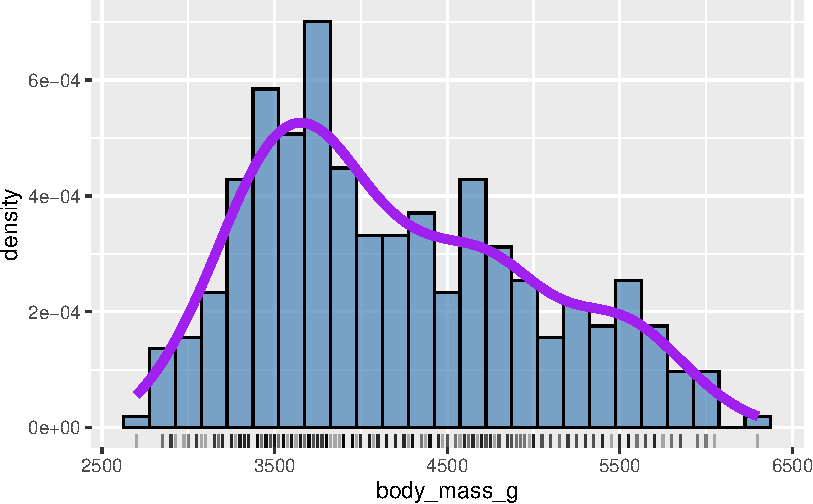
\includegraphics{03-Visualization_files/figure-pdf/unnamed-chunk-25-1.pdf}

C'est plus long, mais c'est tout à fait correct et ça produit exactement
le même résultat qu'auparavant.

\subsection{Les nuages de points et stripcharts}\label{sec-cloud}

Pour ces deux types de graphiques, la variable numérique sera portée par
l'axe des \texttt{y}, et toutes les valeurs seront visibles, de façon
non agrégée (contrairement aux histogrammes où les valeurs individuelles
sont rassemblées à l'intérieur de classes). La différence entre les deux
types de graphiques tient à la nature des informations qui figureront
sur l'axe des \texttt{x} :

\begin{itemize}
\tightlist
\item
  Pour les nuages de points, l'axe des \texttt{x} portera simplement
  l'information du numéro d'observation pour chaque individu. L'individu
  placé sur la première ligne du tableau de données portera l'indice
  \texttt{1}. L'individu placé sur la deuxième ligne du tableau de
  données portera l'indice \texttt{2}, et ainsi de suite jusqu'à
  l'individu placé sur la dernière ligne du tableau (il portera ici
  l'indice 344 puisque le tableau compte 344 lignes)
\item
  Pour un stripchart, l'axe des \texttt{x} portera une unique valeur, la
  même pour tous les individus
\end{itemize}

Dans les deux cas, l'axe des \texttt{x} ne nous sera pas vraiment utile.
Il nous servira simplement à afficher des points sur un graphique, mais
puisque nous ne disposons que d'une unique variable, c'est bien l'axe
des \texttt{y} qui nous intéressera en priorité. Pour faire un nuage de
points, on utilise \texttt{geom\_point()}, et pour un stripchart
\texttt{geom\_jitter()}. Commençons par examiner le nuage de points pour
la variable \texttt{body-mass-g} :

\begin{Shaded}
\begin{Highlighting}[]
\FunctionTok{ggplot}\NormalTok{(penguins, }\FunctionTok{aes}\NormalTok{(}\AttributeTok{x =} \FunctionTok{seq\_along}\NormalTok{(body\_mass\_g), }\AttributeTok{y =}\NormalTok{ body\_mass\_g)) }\SpecialCharTok{+}
  \FunctionTok{geom\_point}\NormalTok{()}
\end{Highlighting}
\end{Shaded}

\begin{verbatim}
Warning: Removed 2 rows containing missing values or values outside the scale range
(`geom_point()`).
\end{verbatim}

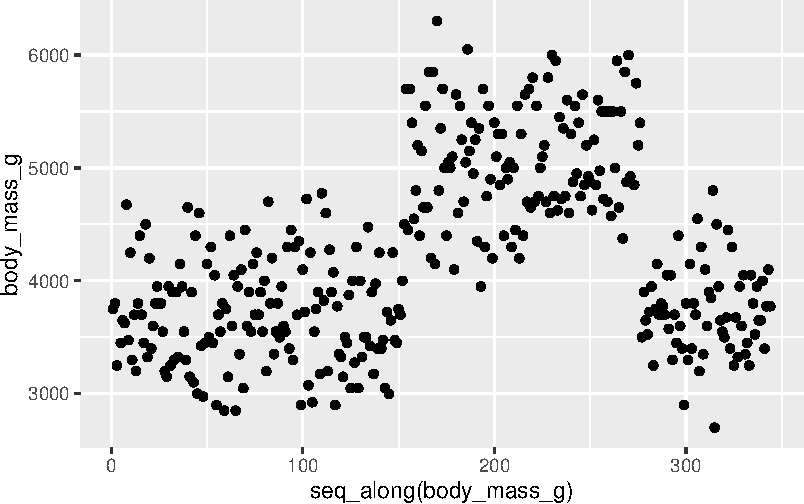
\includegraphics{03-Visualization_files/figure-pdf/unnamed-chunk-26-1.pdf}

C'est la fonction \texttt{seq\_along()}, que l'on associe à l'axe des
\texttt{x}, qui permet de faire apparaître les numéros de lignes du
tableau \texttt{penguins}. On constate ici que 3 groupes de points sont
présents :

\begin{enumerate}
\def\labelenumi{\arabic{enumi}.}
\tightlist
\item
  Pour les lignes 1 à 150 (environ), un premier groupe de points
  présente des masses comprises entre 3000 et 4800 grammes environ.
\item
  Pour les lignes 151 à 275 (environ), un second groupes de points
  présente des masses comprises entre 4000 et plus de 6000 grammes.
\item
  Pour les lignes 276 à 344 (environ), un troisième groupe de points
  présente des valeurs similaires à celles du premier groupe.
\end{enumerate}

En examinant le tableau \texttt{penguins} de plus près, on se rend
compte que les 3 espèces de manchots sont présentées dans l'ordre.
Ainsi, ces 3 groupes correspondent à 3 espèces différentes. Pour le
visualiser, il suffit d'associer la variable \texttt{species} à la
couleur des points. Puisqu'on cherche à associer une variable du tableau
de données à une caractéristique esthétique d'un objet géométrique, on
renseigne \texttt{color\ =\ species} à l'intérieur de \texttt{aes()} :

\begin{Shaded}
\begin{Highlighting}[]
\FunctionTok{ggplot}\NormalTok{(penguins, }\FunctionTok{aes}\NormalTok{(}\AttributeTok{x =} \FunctionTok{seq\_along}\NormalTok{(body\_mass\_g), }\AttributeTok{y =}\NormalTok{ body\_mass\_g)) }\SpecialCharTok{+}
  \FunctionTok{geom\_point}\NormalTok{(}\FunctionTok{aes}\NormalTok{(}\AttributeTok{color =}\NormalTok{ species))}
\end{Highlighting}
\end{Shaded}

\begin{verbatim}
Warning: Removed 2 rows containing missing values or values outside the scale range
(`geom_point()`).
\end{verbatim}

\begin{figure}[H]

\centering{

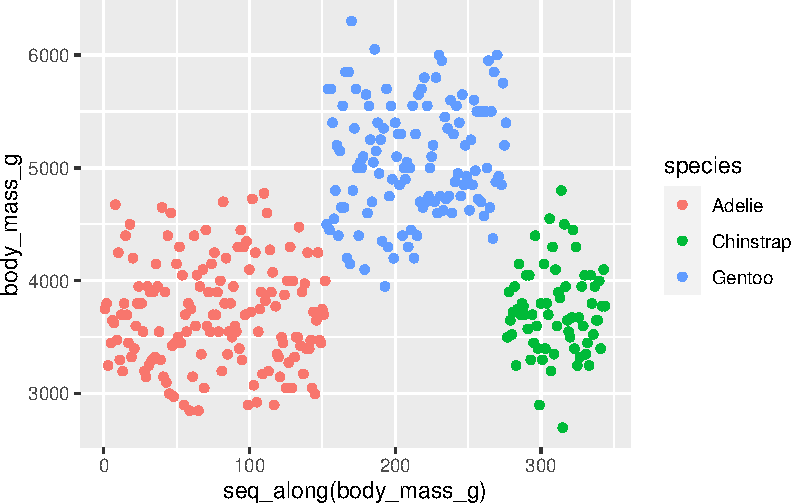
\includegraphics{03-Visualization_files/figure-pdf/fig-cloud-1.pdf}

}

\caption{\label{fig-cloud}Nuage de points des masses corporelles des 3
espèces de manchots}

\end{figure}%

Attention, nous ne sommes déjà plus dans la situation d'une unique
variable numérique : nous avons ici visualisé 2 variables : une
numérique (portée par l'axe des \texttt{y}) et une catégorielle
(l'espèce représentée par la couleur des points). Ici, on constate que
les espèces Adélie et Chinstrap semblent avoir approximativement la même
gamme de masses, alors que les Gentoo semblent nettement plus lourds.

Comme pour les histogrammes, on peut utiliser des caractéristiques
esthétiques variées pour modifier l'apparence des points :

\begin{itemize}
\tightlist
\item
  \texttt{alpha} : la transparence. Choisir une valeur comprise entre 0
  (invisible) et 1 (totalement opaque)
\item
  \texttt{size} : la taille des points
\item
  \texttt{color} : la couleur des points (ou de leur contour pour les
  symboles qui permettent de spécifier une couleur de remplissage et une
  couleur de contour)
\item
  \texttt{fill} : la couleur de remplissage des points (pour les
  symboles qui permettent de spécifier une couleur de remplissage et une
  couleur de contour)
\item
  \texttt{shape} : pour modifier les symboles utilisés. Les symboles
  possibles sont codés ainsi :
\end{itemize}

\begin{figure}

\centering{

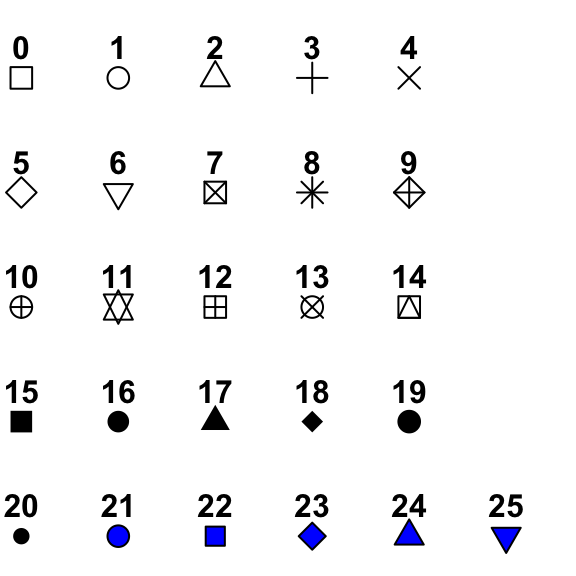
\includegraphics[width=0.5\textwidth,height=\textheight]{images/pch.png}

}

\caption{\label{fig-pch}Liste des symboles et codes correspondants pour
les graphiques faisant apparaître des points. Pour les symboles 21 à 25,
il sera possible de spécifier une couleur de remplissage \texttt{fill}
et une couleur de contour \texttt{color}. Pour tous les autres symboles,
les changements de couleurs se feront avec l'argument \texttt{color}.}

\end{figure}%

Chacune de ces caractéristiques esthétiques peut être associée à une
variable d'un tableau (il faut alors le spécifier à l'intérieur de
\texttt{aes()}), ou à une valeur unique, constante et identique pour
tous les points du graphique (il faut alors le spécifier à l'extérieur
de \texttt{aes()}). Par exemple :

\begin{Shaded}
\begin{Highlighting}[]
\FunctionTok{ggplot}\NormalTok{(penguins, }\FunctionTok{aes}\NormalTok{(}\AttributeTok{x =} \FunctionTok{seq\_along}\NormalTok{(body\_mass\_g), }\AttributeTok{y =}\NormalTok{ body\_mass\_g)) }\SpecialCharTok{+}
  \FunctionTok{geom\_point}\NormalTok{(}\AttributeTok{shape =} \DecValTok{23}\NormalTok{, }\AttributeTok{fill =} \StringTok{"steelblue"}\NormalTok{, }\AttributeTok{color =} \StringTok{"black"}\NormalTok{, }
             \AttributeTok{size =} \DecValTok{3}\NormalTok{, }\AttributeTok{alpha =} \FloatTok{0.5}\NormalTok{)}
\end{Highlighting}
\end{Shaded}

\begin{verbatim}
Warning: Removed 2 rows containing missing values or values outside the scale range
(`geom_point()`).
\end{verbatim}

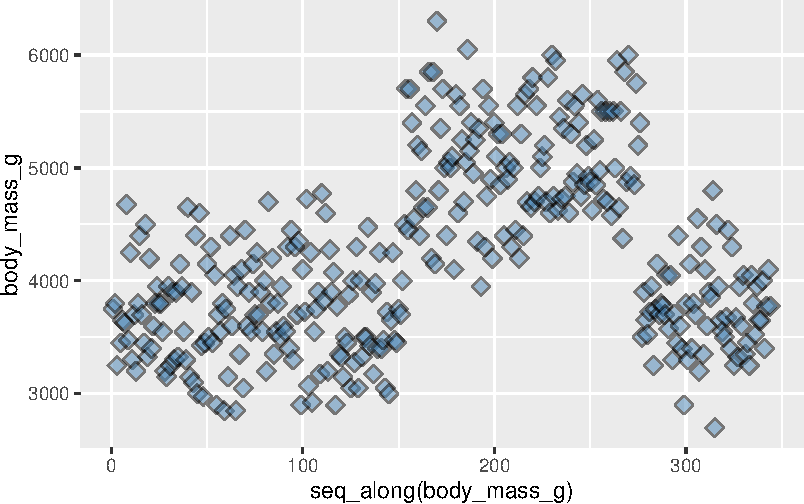
\includegraphics{03-Visualization_files/figure-pdf/unnamed-chunk-28-1.pdf}

L'ajout de la transparence permet de régler le problème des points qui
se superposent (un phénomène nommé ``overplotting'').

Examinons à présent un exemple de stripchart :

\begin{Shaded}
\begin{Highlighting}[]
\FunctionTok{ggplot}\NormalTok{(penguins, }\FunctionTok{aes}\NormalTok{(}\AttributeTok{x =} \StringTok{""}\NormalTok{, }\AttributeTok{y =}\NormalTok{ body\_mass\_g)) }\SpecialCharTok{+}
  \FunctionTok{geom\_jitter}\NormalTok{()}
\end{Highlighting}
\end{Shaded}

\begin{verbatim}
Warning: Removed 2 rows containing missing values or values outside the scale range
(`geom_point()`).
\end{verbatim}

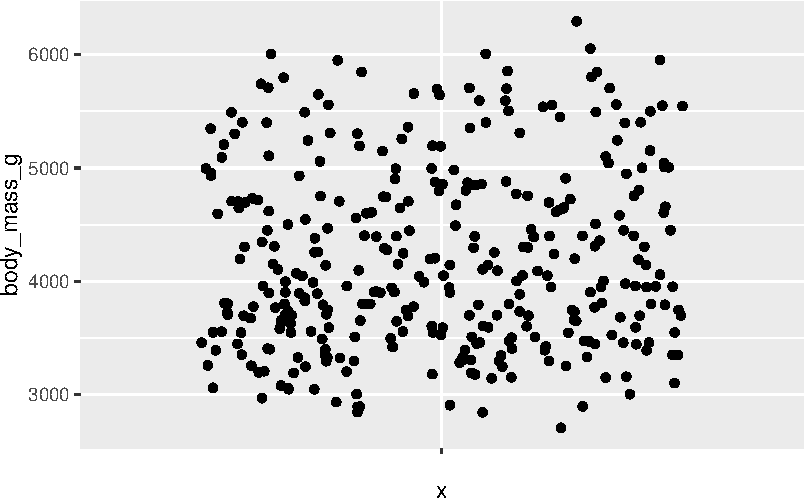
\includegraphics{03-Visualization_files/figure-pdf/unnamed-chunk-29-1.pdf}

En indiquant \texttt{x\ =\ ""}, nous créons une unique catégorie pour
l'axe des abscisses, qui sera utilisée pour placer les valeurs de tous
les individus. Les valeurs de \texttt{body\_mass\_g} sont lues sur l'axe
des \texttt{y}, comme pour un nuage de point classique. Si les points
apparaissent dispersés, c'est en raison de 2 arguments spécifiques de la
fonction \texttt{geom\_jitter()} :

\begin{itemize}
\tightlist
\item
  \texttt{width\ =} permet de spécifier l'étendue horizontale du bruit
  aléatoire qui sera utilisé pour placer les points
\item
  \texttt{height\ =} permet de spécifier l'étendue verticale du bruit
  aléatoire qui sera utilisé pour placer les points
\end{itemize}

Si nous ne renseignons pas nous même ces deux arguments, ils sont fixés
automatiquement par le logiciel, ce qui n'est pas souhaitable, notamment
pour le bruit vertical. Pour mieux comprendre, voyons ce qui se passe
dans 3 situations :

\begin{Shaded}
\begin{Highlighting}[]
\FunctionTok{ggplot}\NormalTok{(penguins, }\FunctionTok{aes}\NormalTok{(}\AttributeTok{x =} \StringTok{""}\NormalTok{, }\AttributeTok{y =}\NormalTok{ body\_mass\_g)) }\SpecialCharTok{+}
  \FunctionTok{geom\_jitter}\NormalTok{(}\AttributeTok{width =} \DecValTok{0}\NormalTok{, }\AttributeTok{height =} \DecValTok{0}\NormalTok{)}

\FunctionTok{ggplot}\NormalTok{(penguins, }\FunctionTok{aes}\NormalTok{(}\AttributeTok{x =} \StringTok{""}\NormalTok{, }\AttributeTok{y =}\NormalTok{ body\_mass\_g)) }\SpecialCharTok{+}
  \FunctionTok{geom\_jitter}\NormalTok{(}\AttributeTok{width =} \FloatTok{0.1}\NormalTok{, }\AttributeTok{height =} \DecValTok{0}\NormalTok{)}

\FunctionTok{ggplot}\NormalTok{(penguins, }\FunctionTok{aes}\NormalTok{(}\AttributeTok{x =} \StringTok{""}\NormalTok{, }\AttributeTok{y =}\NormalTok{ body\_mass\_g)) }\SpecialCharTok{+}
  \FunctionTok{geom\_jitter}\NormalTok{(}\AttributeTok{width =} \FloatTok{0.1}\NormalTok{, }\AttributeTok{height =} \DecValTok{2000}\NormalTok{)}
\end{Highlighting}
\end{Shaded}

\begin{figure}

\begin{minipage}{0.33\linewidth}

\centering{

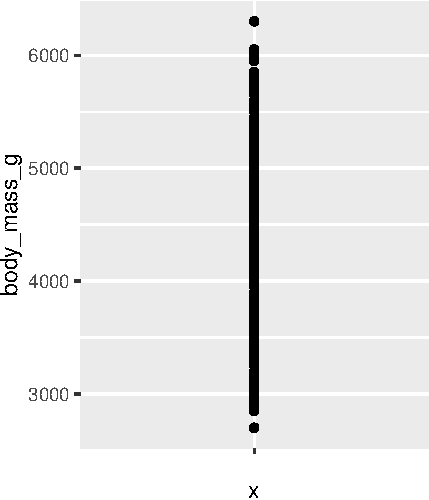
\includegraphics{03-Visualization_files/figure-pdf/fig-jitter-1.pdf}

}

\subcaption{\label{fig-jitter-1}Pas de dispersion horizontale, pas de
dispersion verticale}

\end{minipage}%
%
\begin{minipage}{0.33\linewidth}

\centering{

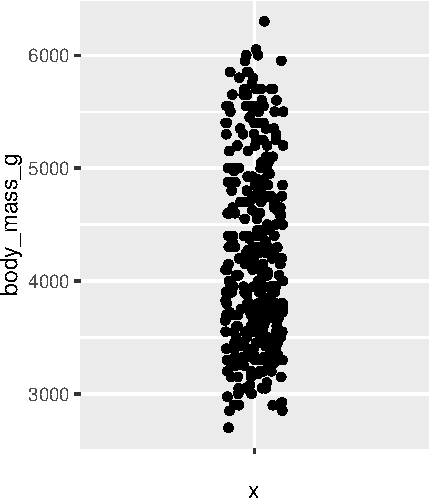
\includegraphics{03-Visualization_files/figure-pdf/fig-jitter-2.pdf}

}

\subcaption{\label{fig-jitter-2}Faible dispersion horizontale, pas de
dispersion verticale}

\end{minipage}%
%
\begin{minipage}{0.33\linewidth}

\centering{

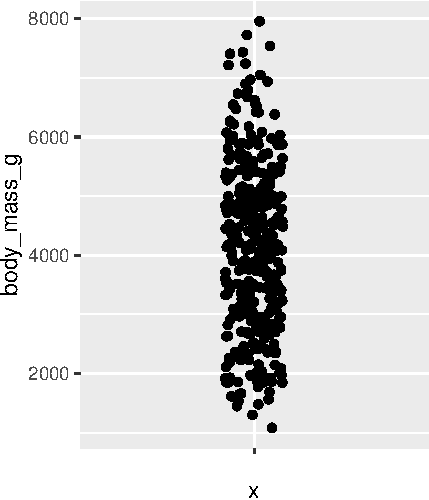
\includegraphics{03-Visualization_files/figure-pdf/fig-jitter-3.pdf}

}

\subcaption{\label{fig-jitter-3}Faible dispersion horizontale, forte
dispersion verticale}

\end{minipage}%

\caption{\label{fig-jitter}Trois exemples de stripchart}

\end{figure}%

\begin{itemize}
\item
  Le premier exemple (Figure~\ref{fig-jitter-1}) ne présente aucune
  dispersion, ni horizontale (\texttt{width\ =\ 0}), ni verticale
  (\texttt{height\ =\ 0}). Les points apparaissent donc tous alignés,
  ils ont en effet tous la même valeur sur l'axe des abscisses. Leur
  position sur l'axe des \texttt{y} reflète la masse réellement observée
  pour chaque individu. Cette façon de représenter les données n'est pas
  très utile car la superposition des points vient empêcher la
  visualisation correcte de la distribution : ici, il est impossible de
  dire quelles sont les masses les plus fréquemment observées ou les
  plus rarement observées.
\item
  Le second exemple (Figure~\ref{fig-jitter-2}) présente une dispersion
  horizontale modérée (\texttt{width\ =\ 0.1}) et pas de dispersion
  verticale (\texttt{height\ =\ 0}). Ici, tous les points ne sont plus
  alignés sur une seule droite. Puisque nous avons fixé
  \texttt{width\ =\ 0.1}, la position horizontale des points est choisie
  aléatoirement par \texttt{R} : il ajoute un léger bruit horizontal
  aléatoire, soit positif, soit négatif, avant de placer les points le
  long de l'axe des abscisses. Plus la valeur de \texttt{width} sera
  élevée, plus l'étendue du bruit horizontal sera importante. Sur l'axe
  des \texttt{y} en revanche, aucun bruit n'a été ajouté
  (\texttt{height\ =\ 0}). La position des points le long de cet axe
  reflète donc parfaitement la masse de chaque individu telle
  qu'enregistrées dans le tableau \texttt{penguins} et c'est bien ce que
  nous voulons. D'ailleurs, on constate que l'axe des ordonnées est
  strictement identique (même étendue, même graduations\ldots) pour les
  2 premiers sous-graphiques. C'est ce type de représentation que nous
  recherchons. En effet, l'absence de bruit vertical nous permet de
  visualiser correctement (donc sans distorsion) la variable numérique
  choisie (ici \texttt{body\_mass\_g}), et le bruit horizontal nous
  permet d'étaler légèrement les points de part et d'autres d'un axe
  vertical virtuel, ce qui a pour effet de réduire l'overplotting, et ce
  qui nous permet donc de visualiser les zones où les points sont plus
  nombreux/denses et les zones où les observations sont plus rares. Ici,
  on observe une majorité de points entre 3000 et 4000 grammes, une
  densité de points intermédiaire entre 4000 et 5000 grammes, et des
  points moins nombreux (donc moins d'individus) pour les masses
  supérieures à 5000 grammes.
\item
  Le troisième exemple (Figure~\ref{fig-jitter-3}) présente une
  dispersion horizontale modérée (\texttt{width\ =\ 0.1}) et une
  importante dispersion verticale (\texttt{height\ =\ 2000}). Cela
  signifie que la position des points sur l'axe des \texttt{y} ne
  reflète plus les vraies valeurs de masses enregistrées dans le tableau
  \texttt{penguins}, mais des valeurs de masses auxquelles un bruit
  aléatoire a été ajouté ou retiré. C'est ce qui explique que l'axe des
  ordonnées ne présente pas la même échelle que pour les 2 autres
  graphiques. Ce n'est évidemment pas souhaitable, car si nous voulons
  bel et bien ajouter un bruit horizontal pour éviter la superposition
  des points, il est essentiel de ne pas modifier la position verticale
  des points qui nous renseigne sur la variable d'intérêt. Ici, la
  Figure~\ref{fig-jitter-3} présente un axe des \texttt{y} différent des
  2 autres sous-figures, et la position verticale des points a été
  tellement altérée qu'on ne peut plus distinguer la sur-abondance de
  données entre 3000 et 4000 grammes, ni la sous-représentation des
  observations au-dessus de 5000 grammes. Il sera donc important à
  l'avenir de toujours fixer \texttt{height\ =\ 0} pour faire un
  stripchart correct.
\end{itemize}

\begin{tcolorbox}[enhanced jigsaw, colbacktitle=quarto-callout-important-color!10!white, colframe=quarto-callout-important-color-frame, bottomtitle=1mm, opacityback=0, arc=.35mm, leftrule=.75mm, titlerule=0mm, colback=white, title=\textcolor{quarto-callout-important-color}{\faExclamation}\hspace{0.5em}{Important}, toptitle=1mm, breakable, coltitle=black, rightrule=.15mm, left=2mm, opacitybacktitle=0.6, toprule=.15mm, bottomrule=.15mm]

Sur un stripchart :

\begin{itemize}
\tightlist
\item
  la position \textbf{verticale} des points ne doit jamais être
  modifiée. On fixera donc toujours \texttt{height\ =\ 0}
\item
  la position \textbf{horizontale} des points doit être modifiée afin
  d'éviter l'overplotting et de visualiser les zones de fortes et
  faibles densités de points. On choisira donc en général des valeurs de
  \texttt{width} comprises entre \texttt{0.1} et \texttt{0.4}
\end{itemize}

\end{tcolorbox}

Enfin, puisqu'un stripchart permet d'afficher des points sur un
graphiques, les arguments permettant de modifier l'aspect des points
sont les mêmes que pour les nuages de points. Par exemple :

\begin{Shaded}
\begin{Highlighting}[]
\FunctionTok{ggplot}\NormalTok{(penguins, }\FunctionTok{aes}\NormalTok{(}\AttributeTok{x =} \StringTok{""}\NormalTok{, }\AttributeTok{y =}\NormalTok{ body\_mass\_g)) }\SpecialCharTok{+}
  \FunctionTok{geom\_jitter}\NormalTok{(}\FunctionTok{aes}\NormalTok{(}\AttributeTok{color =}\NormalTok{ species, }\AttributeTok{shape =}\NormalTok{ species),}
              \AttributeTok{size =} \DecValTok{3}\NormalTok{, }\AttributeTok{alpha =} \FloatTok{0.6}\NormalTok{, }
              \AttributeTok{width =} \FloatTok{0.1}\NormalTok{, }\AttributeTok{height =} \DecValTok{0}\NormalTok{)}
\end{Highlighting}
\end{Shaded}

\begin{verbatim}
Warning: Removed 2 rows containing missing values or values outside the scale range
(`geom_point()`).
\end{verbatim}

\begin{figure}[H]

\centering{

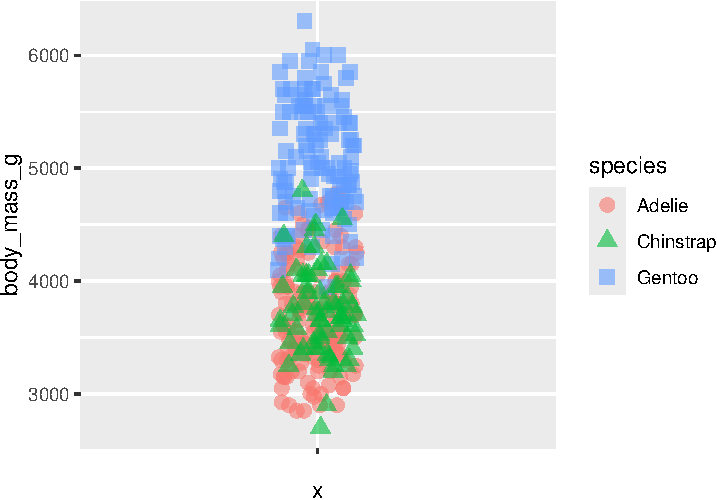
\includegraphics{03-Visualization_files/figure-pdf/fig-strip-1.pdf}

}

\caption{\label{fig-strip}Un exemple de stripchart}

\end{figure}%

Sur cette figure, comme pour le nuage de points réalisé plus haut, j'ai
associé la variable \texttt{species} à la couleur des points (donc à
l'intérieur de \texttt{aes()}). J'ai également associé cette variable à
la forme des points \texttt{shape\ =\ species} à l'intérieur de
\texttt{aes()}. C'est ce qui explique que chacune des 3 espèces apparaît
sous la forme de symboles de formes et de couleurs différents. Pour
limiter l'overplotting, j'ai spécifié un bruit horizontal, et j'ai fixé
le bruit vertical à zéro. Enfin j'ai augmenté la taille des symboles
(avec \texttt{size\ =\ 3}, en dehors de \texttt{aes()} car \texttt{3}
est une constante qui s'appliquera à tous les points du graphique de la
même manière) et leur transparence (avec \texttt{alpha\ =\ 0.6},
toujours en dehors de \texttt{aes()} pour la même raison). On constate
ici encore que les masses corporelles des manchots Adélie et Chinstrap
sont très similaires, et inférieures à celles de l'espèce Gentoo.

\subsection{Exercices}\label{sec-exo-4}

\begin{enumerate}
\def\labelenumi{\arabic{enumi}.}
\item
  À quoi sert l'argument \texttt{stroke} pour les nuages de points et
  les stripcharts ?
\item
  Créez de nouveaux graphiques (histogramme et diagramme de densité)
  avec la variable contenant l'information de la longueur des nageoires
  des manchots \texttt{flipper\_length\_mm}. Décrivez les graphiques
  obtenus. Vos observations sont-elles cohérentes avec ce que nous
  savons maintenant des masses individuelles ?
\item
  Visualisez ces données avec un nuage de points ou un stripchart.
  Retrouvez-vous les mêmes informations de distribution ?
\end{enumerate}

\section{Une seule variable
catégorielle}\label{une-seule-variable-catuxe9gorielle}

\subsection{Les diagrammes bâtons}\label{les-diagrammes-buxe2tons}

Comme nous l'avons vu plus haut, les histogrammes permettent de
visualiser la distribution d'une \textbf{variable numérique continue}.
Souvent, on souhaite visualiser la distribution d'une \textbf{variable
catégorielle}. C'est une tâche relativement aisée puisqu'elle consiste
simplement à compter combien d'éléments tombent dans chacune des
catégories (ou modalités) de la variable catégorielle. Le meilleur moyen
de visualiser de telles données de comptage (\emph{aka} fréquences) est
de réaliser un diagramme bâtons, autrement appelé \textbf{barplot} ou
\textbf{barchart}.

Une difficulté, toutefois, concerne la façon dont les données sont
présentées : est-ce que la variable d'intérêt est ``pré-comptée'' ou non
? Par exemple, le code ci-dessous crée 2 \texttt{data.frame} qui
représentent la même collection de fruits : 3 pommes, 2 oranges et 4
bananes :

\begin{Shaded}
\begin{Highlighting}[]
\NormalTok{panier }\OtherTok{\textless{}{-}} \FunctionTok{tibble}\NormalTok{(}
  \AttributeTok{fruit =} \FunctionTok{c}\NormalTok{(}\StringTok{"pomme"}\NormalTok{, }\StringTok{"pomme"}\NormalTok{, }\StringTok{"banane"}\NormalTok{, }\StringTok{"pomme"}\NormalTok{, }\StringTok{"orange"}\NormalTok{, }\StringTok{"banane"}\NormalTok{, }\StringTok{"orange"}\NormalTok{, }\StringTok{"banane"}\NormalTok{, }\StringTok{"banane"}\NormalTok{)}
\NormalTok{)}

\NormalTok{panier\_counted }\OtherTok{\textless{}{-}} \FunctionTok{tibble}\NormalTok{(}
  \AttributeTok{fruit =} \FunctionTok{c}\NormalTok{(}\StringTok{"pomme"}\NormalTok{, }\StringTok{"orange"}\NormalTok{, }\StringTok{"banane"}\NormalTok{),}
  \AttributeTok{nombre =} \FunctionTok{c}\NormalTok{(}\DecValTok{3}\NormalTok{, }\DecValTok{2}\NormalTok{, }\DecValTok{4}\NormalTok{)}
\NormalTok{)}
\end{Highlighting}
\end{Shaded}

Le tableau \texttt{panier} contient des données qui n'ont pas encore été
comptées. Le tableau contient donc une unique variable nommée
\texttt{fruit} :

\begin{Shaded}
\begin{Highlighting}[]
\NormalTok{panier}
\end{Highlighting}
\end{Shaded}

\begin{verbatim}
# A tibble: 9 x 1
  fruit 
  <chr> 
1 pomme 
2 pomme 
3 banane
4 pomme 
5 orange
6 banane
7 orange
8 banane
9 banane
\end{verbatim}

À l'inverse, le tableau \texttt{panier\_counted} contient des données
qui ont déjà été comptées. Le tableau contient donc 2 variables dans 2
colonnes distinctes : une colonne \texttt{fruit} et une colonne
\texttt{nombre}, mais seulement 3 lignes puisque seulement 3 modalités
(les catégories de la variable catégorielle) sont présentes pour la
variable \texttt{fruit} :

\begin{Shaded}
\begin{Highlighting}[]
\NormalTok{panier\_counted}
\end{Highlighting}
\end{Shaded}

\begin{verbatim}
# A tibble: 3 x 2
  fruit  nombre
  <chr>   <dbl>
1 pomme       3
2 orange      2
3 banane      4
\end{verbatim}

Les deux tableaux \texttt{panier} et \texttt{panier\_counted}
représentent exactement les mêmes données, mais sous deux formats
différents. Du fait de ces deux formats possibles, deux objets
géométriques distincts devront être utilisés pour représenter les
données. Le graphique obtenu sera le même, mais à chaque format de
tableau son \texttt{geom\_...()}.

\subsubsection{\texorpdfstring{\texttt{geom\_bar()} et
\texttt{geom\_col()}}{geom\_bar() et geom\_col()}}\label{geom_bar-et-geom_col}

Pour visualiser les données non pré-comptées, on utilise
\texttt{geom\_bar()} :

\begin{Shaded}
\begin{Highlighting}[]
\FunctionTok{ggplot}\NormalTok{(panier, }\FunctionTok{aes}\NormalTok{(}\AttributeTok{x =}\NormalTok{ fruit)) }\SpecialCharTok{+}
  \FunctionTok{geom\_bar}\NormalTok{()}
\end{Highlighting}
\end{Shaded}

\begin{figure}[H]

\centering{

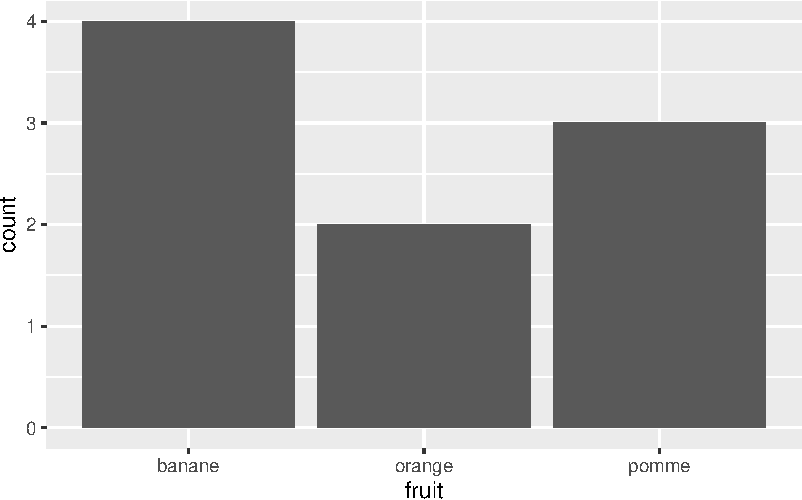
\includegraphics{03-Visualization_files/figure-pdf/fig-barplot-1.pdf}

}

\caption{\label{fig-barplot}Barplot pour des données non pré-comptées.}

\end{figure}%

Pour visualiser les données déjà pré-comptées, on utilise
\texttt{geom\_col()} :

\begin{Shaded}
\begin{Highlighting}[]
\FunctionTok{ggplot}\NormalTok{(panier\_counted, }\FunctionTok{aes}\NormalTok{(}\AttributeTok{x =}\NormalTok{ fruit, }\AttributeTok{y =}\NormalTok{ nombre)) }\SpecialCharTok{+}
  \FunctionTok{geom\_col}\NormalTok{()}
\end{Highlighting}
\end{Shaded}

\begin{figure}[H]

\centering{

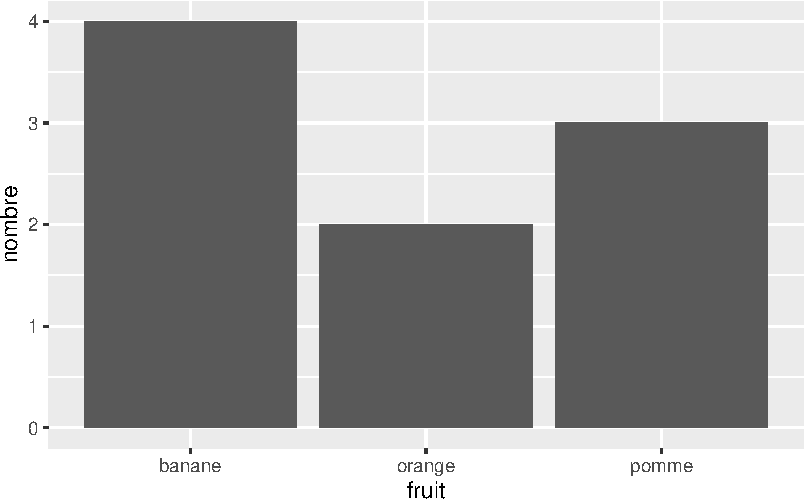
\includegraphics{03-Visualization_files/figure-pdf/fig-barplotcol-1.pdf}

}

\caption{\label{fig-barplotcol}Barplot pour des données pré-comptées.}

\end{figure}%

Notez que les figures Figure~\ref{fig-barplot} et
Figure~\ref{fig-barplotcol} sont absolument identiques (à l'exception du
titre de l'axe des ordonnées), mais qu'elles ont été créées à partir de
2 tableaux de données différents. En particulier, notez que :

\begin{itemize}
\tightlist
\item
  Le code qui génère la figure Figure~\ref{fig-barplot} utilise le jeu
  de données \texttt{panier}, et n'associe pas de variable à l'axe des
  ordonnées : dans la fonction \texttt{aes()}, seule la variable
  associée à \texttt{x} est précisée. C'est la fonction
  \texttt{geom\_bar()} qui calcule automatiquement les abondances (ou
  fréquences) pour chaque catégorie de la variable \texttt{fruit}. La
  variable \texttt{count} est ainsi générée automatiquement et associée
  à \texttt{y}.
\item
  Le code qui génère la figure Figure~\ref{fig-barplotcol} utilise le
  jeu de données \texttt{panier\_counted}. Ici, c'est bien l'utilisateur
  qui associe la variable \texttt{nombre} à l'axe des \texttt{y} à
  l'intérieur de la fonction \texttt{aes()}. La fonction
  \texttt{geom\_col()} a besoin de 2 variables (une variable
  catégorielle pour l'axe des \texttt{x} et une numérique pour l'axe des
  \texttt{y}) pour fonctionner.
\end{itemize}

Autrement dit, lorsque vous souhaiterez créer un diagramme bâtons, il
faudra donc au préalable vérifier de quel type de données vous disposez
pour choisir l'objet géométrique approprié :

\begin{tcolorbox}[enhanced jigsaw, colbacktitle=quarto-callout-important-color!10!white, colframe=quarto-callout-important-color-frame, bottomtitle=1mm, opacityback=0, arc=.35mm, leftrule=.75mm, titlerule=0mm, colback=white, title=\textcolor{quarto-callout-important-color}{\faExclamation}\hspace{0.5em}{Diagrammes bâtons}, toptitle=1mm, breakable, coltitle=black, rightrule=.15mm, left=2mm, opacitybacktitle=0.6, toprule=.15mm, bottomrule=.15mm]

\begin{itemize}
\tightlist
\item
  Si la variable catégorielle n'est pas pré-comptée dans le tableau de
  données \faIcon{arrow-right} \texttt{geom\_bar()}. La variable
  catégorielle est associée à l'esthétique \texttt{x} du graphique. On
  ne renseigne pas \texttt{y}.
\item
  Si la variable catégorielle est pré-comptée dans le tableau de données
  \faIcon{arrow-right} \texttt{geom\_col()}. La variable catégorielle
  est associée à l'esthétique \texttt{x} du graphique. On associe
  explicitement les comptages à l'esthétique \texttt{y} du graphique.
\end{itemize}

\end{tcolorbox}

Enfin, notez que l'ordre des modalité (ou catégories) qui apparaissent
sur l'axe des abscisses est l'ordre alphabétique : la modalité
\texttt{banane} apparaît à gauche, puis la modalité \texttt{orange} et
enfin la modalité \texttt{pomme}. Bien souvent, cet ordre alphabétique
n'est pas pertinent. Nous verrons plus loin comment faire pour trier les
catégories par ordre croissant ou décroissant. C'est en effet une
possibilité intéressante qui est impossible pour les histogrammes (car
l'axe des \texttt{x} porte une variable numérique continue qu'il est
impossible de ``mélanger''), mais souvent vivement recommandée pour les
diagrammes bâtons.

\subsubsection{Un exemple concret}\label{un-exemple-concret}

Revenons aux manchots. Imaginons que nous souhaitions connaître le
nombre d'individus étudiés pour chaque espèce. Dans le jeu de données
\texttt{penguins}, la variable \texttt{species} indique à quelle espèce
appartiennent chacun des 344 individus étudiés. Une façon simple de
représenter ces données est donc la suivante :

\begin{Shaded}
\begin{Highlighting}[]
\FunctionTok{ggplot}\NormalTok{(penguins, }\FunctionTok{aes}\NormalTok{(}\AttributeTok{x =}\NormalTok{ species)) }\SpecialCharTok{+}
  \FunctionTok{geom\_bar}\NormalTok{()}
\end{Highlighting}
\end{Shaded}

\begin{figure}[H]

\centering{

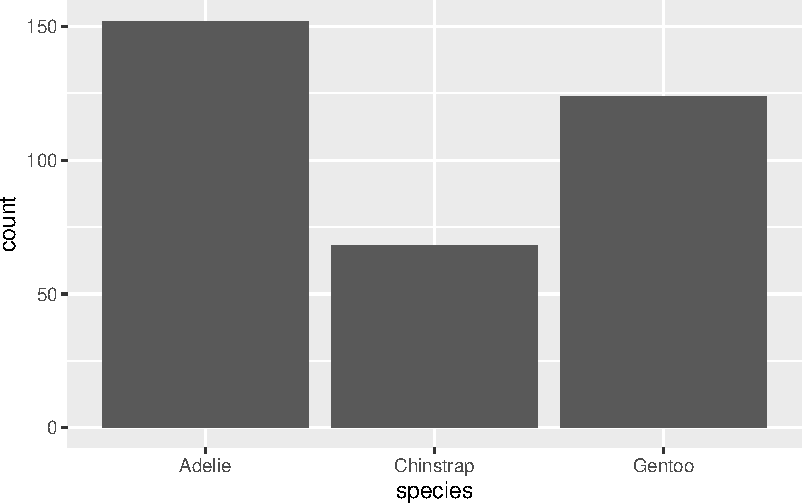
\includegraphics{03-Visualization_files/figure-pdf/fig-bpspecies-1.pdf}

}

\caption{\label{fig-bpspecies}Effectifs pour les 3 espèces de manchots
étudiées}

\end{figure}%

Ici, \texttt{geom\_bar()} a compté le nombre d'occurrences de chaque
espèce dans le tableau \texttt{penguins} et a automatiquement associé ce
nombre à l'axe des ordonnées.

Là encore, les modalités sont triées par ordre alphabétique sur l'axe
des abscisses. Il est généralement plus utile de trier les catégories
par ordre décroissant. Nous pouvons faire cela facilement grâce à la
fonction \texttt{fct\_infreq()} du package \texttt{forcats}, qui permet
de modifier l'ordre des modalités d'une variable catégorielle (ou
facteur). Si vous avez installé le \texttt{tidyverse}, le package
\texttt{forcast} doit être disponible sur votre ordinateur. N'oubliez
pas de le charger si besoin :

\begin{Shaded}
\begin{Highlighting}[]
\FunctionTok{library}\NormalTok{(forcats)}
\FunctionTok{ggplot}\NormalTok{(penguins, }\FunctionTok{aes}\NormalTok{(}\AttributeTok{x =} \FunctionTok{fct\_infreq}\NormalTok{(species))) }\SpecialCharTok{+}
  \FunctionTok{geom\_bar}\NormalTok{()}
\end{Highlighting}
\end{Shaded}

\begin{figure}[H]

\centering{

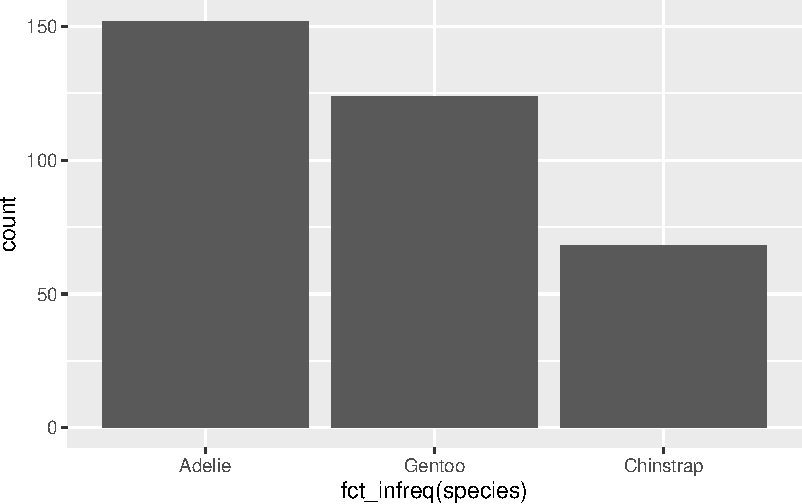
\includegraphics{03-Visualization_files/figure-pdf/fig-bpspecies-infreq-1.pdf}

}

\caption{\label{fig-bpspecies-infreq}Effectifs pour les 3 espèces de
manchots étudiées, triés en ordre décroissant}

\end{figure}%

Ordonner les catégories par ordre décroissant est souvent indispensable
afin de faciliter la lecture du graphique et les comparaisons entre
catégories.

Si nous souhaitons connaître le nombre précis d'individus de chaque
espèce, il nous faut faire appel à plusieurs fonctions du package
\texttt{dplyr} que nous détaillerons dans le chapitre
Chapitre~\ref{sec-wrangling}. Ci-dessous, nous créons un nouveau tableau
\texttt{species\_table} contenant le nombre d'individus de chaque espèce
et les espèces sont ordonnées par abondance décroissante :

\begin{Shaded}
\begin{Highlighting}[]
\NormalTok{species\_table }\OtherTok{\textless{}{-}}\NormalTok{ penguins }\SpecialCharTok{\%\textgreater{}\%}   \CommentTok{\# On prend le tableau penguins, puis...}
  \FunctionTok{count}\NormalTok{(species) }\SpecialCharTok{\%\textgreater{}\%}            \CommentTok{\# On compte les effectifs de chaque espèce, puis...}
  \FunctionTok{arrange}\NormalTok{(}\FunctionTok{desc}\NormalTok{(n))              }\CommentTok{\# On trie par effectif décroissants ...}
\NormalTok{species\_table                   }\CommentTok{\# Enfin, on affiche la nouvelle table}
\end{Highlighting}
\end{Shaded}

\begin{verbatim}
# A tibble: 3 x 2
  species       n
  <fct>     <int>
1 Adelie      152
2 Gentoo      124
3 Chinstrap    68
\end{verbatim}

Ici, la table a été triée par effectifs décroissants. Mais attention,
\textbf{les niveaux} du facteur \texttt{species} n'ont pas été modifiés
:

\begin{Shaded}
\begin{Highlighting}[]
\FunctionTok{factor}\NormalTok{(species\_table}\SpecialCharTok{$}\NormalTok{species)}
\end{Highlighting}
\end{Shaded}

\begin{verbatim}
[1] Adelie    Gentoo    Chinstrap
Levels: Adelie Chinstrap Gentoo
\end{verbatim}

Le premier niveau est toujours \texttt{Adélie}, puis \texttt{Chinstrap},
en enfin \texttt{Gentoo}, et non pas l'ordre du tableau nouvellement
créé (\texttt{Adelie}, puis \texttt{Gentoo}, puis \texttt{Chinstrap})
car les niveaux sont toujours triés par ordre alphabétique. La
conséquence est que si nous devions faire un diagramme bâtons avec ces
données, la fonction \texttt{geom\_col()} ne permettrait pas d'ordonner
les catégories correctement :

\begin{Shaded}
\begin{Highlighting}[]
\FunctionTok{ggplot}\NormalTok{(species\_table, }\FunctionTok{aes}\NormalTok{(}\AttributeTok{x =}\NormalTok{ species, }\AttributeTok{y =}\NormalTok{ n)) }\SpecialCharTok{+}
  \FunctionTok{geom\_col}\NormalTok{()}
\end{Highlighting}
\end{Shaded}

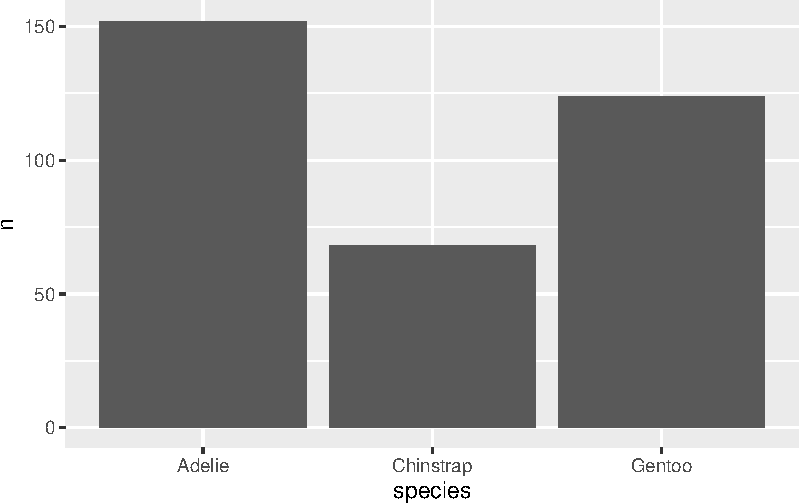
\includegraphics{03-Visualization_files/figure-pdf/unnamed-chunk-42-1.pdf}

Si nous souhaitons trier ces catégories par effectif décroissant, la
fonction \texttt{fct\_infreq()} ne nous est ici d'aucune utilité. En
effet, le tableau \texttt{species\_table} contient une seule ligne pour
chaque espèce, donc une fréquence de \texttt{1} pour chaque espèce. Le
critère de la fréquence d'occurrence des modalités dans le tableau de
données ne peut donc pas être utilisé. Pour parvenir à nos fins avec ce
tableau déjà précompté, il faut cette fois utiliser la fonction
\texttt{fct\_reorder()} pour ordonner correctement les catégories. Cette
fonction prends 3 arguments :

\begin{enumerate}
\def\labelenumi{\arabic{enumi}.}
\tightlist
\item
  La variable catégorielle dont on souhaite réordonner les niveaux (ici,
  la variable \texttt{species} du tableau \texttt{species\_table}).
\item
  Une variable numérique qui permet d'ordonner les catégories (ici, la
  variable \texttt{n} du même tableau).
\item
  L'argument optionnel \texttt{.desc} qui permet de préciser si le tri
  doit être fait en ordre croissant (c'est le cas par défaut) ou
  décroissant.
\end{enumerate}

\begin{Shaded}
\begin{Highlighting}[]
\FunctionTok{ggplot}\NormalTok{(species\_table, }
       \FunctionTok{aes}\NormalTok{(}\AttributeTok{x =} \FunctionTok{fct\_reorder}\NormalTok{(species, n, }\AttributeTok{.desc =} \ConstantTok{TRUE}\NormalTok{), }\AttributeTok{y =}\NormalTok{ n)) }\SpecialCharTok{+}
  \FunctionTok{geom\_col}\NormalTok{()}
\end{Highlighting}
\end{Shaded}

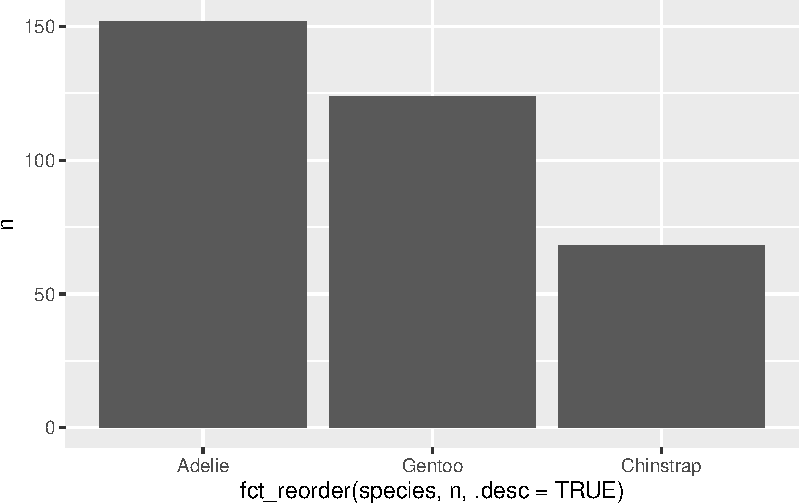
\includegraphics{03-Visualization_files/figure-pdf/unnamed-chunk-43-1.pdf}

Vous voyez donc que selon le type de données dont vous disposez (soit un
tableau comme \texttt{penguins}, avec toutes les observations, soit un
tableau beaucoup plus compact comme \texttt{species\_table}), la
démarche permettant de produire un diagramme bâtons, dans lequel les
catégories seront triées, sera différente.

Une dernière précision : inverser l'ordre des variables sur les axes du
graphiques permet de faire un diagramme bâtons horizontal. C'est parfois
très utile lorsque les modalités de la variable catégorielle sont
nombreuses et/ou que leur nom est long. Faire apparaître les modalités
sur l'axe des \texttt{y} au lieu de l'axe des \texttt{x} peut rendre
leur lecture plus aisée :

\begin{Shaded}
\begin{Highlighting}[]
\FunctionTok{ggplot}\NormalTok{(penguins, }\FunctionTok{aes}\NormalTok{(}\AttributeTok{y =} \FunctionTok{fct\_infreq}\NormalTok{(species))) }\SpecialCharTok{+}
  \FunctionTok{geom\_bar}\NormalTok{(}\AttributeTok{fill =} \StringTok{"steelblue"}\NormalTok{, }\AttributeTok{color =} \StringTok{"black"}\NormalTok{, }\AttributeTok{alpha =} \FloatTok{0.7}\NormalTok{)}
\end{Highlighting}
\end{Shaded}

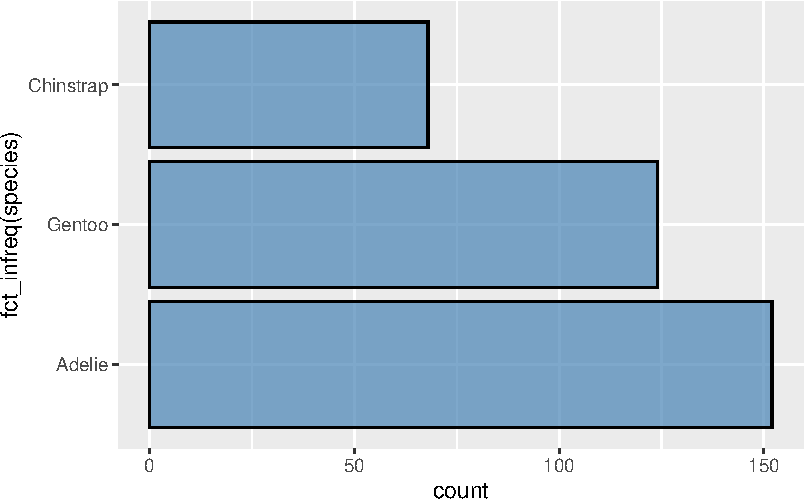
\includegraphics{03-Visualization_files/figure-pdf/unnamed-chunk-44-1.pdf}

\begin{Shaded}
\begin{Highlighting}[]
\FunctionTok{ggplot}\NormalTok{(species\_table, }
       \FunctionTok{aes}\NormalTok{(}\AttributeTok{y =} \FunctionTok{fct\_reorder}\NormalTok{(species, n, }\AttributeTok{.desc =} \ConstantTok{TRUE}\NormalTok{), }\AttributeTok{x =}\NormalTok{ n)) }\SpecialCharTok{+}
  \FunctionTok{geom\_col}\NormalTok{(}\AttributeTok{fill =} \StringTok{"firebrick"}\NormalTok{, }\AttributeTok{color =} \StringTok{"black"}\NormalTok{, }\AttributeTok{alpha =} \FloatTok{0.7}\NormalTok{)}
\end{Highlighting}
\end{Shaded}

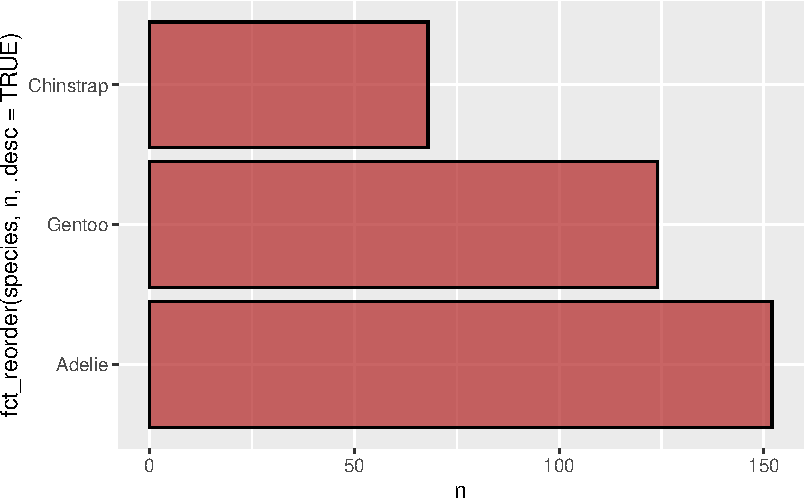
\includegraphics{03-Visualization_files/figure-pdf/unnamed-chunk-44-2.pdf}

\subsubsection{Exercices}\label{sec-exo-6}

\begin{enumerate}
\def\labelenumi{\arabic{enumi}.}
\tightlist
\item
  Quelle est la différence entre un histogramme et un diagramme bâtons ?
\item
  Pourquoi les histogrammes sont-ils inadaptés pour visualiser des
  données catégorielles ?
\item
  Pourquoi ne peut-on pas trier un histogramme par ordre croissant ?
\item
  Quelle île de l'archipel Palmer a fourni le plus grand nombre de
  manchots pour cette étude ?
\end{enumerate}

\subsection{Éviter à tout prix les diagrammes
circulaires}\label{sec-pie}

À mon grand désarroi, l'un des graphiques classiquement utilisé pour
représenter la distribution d'une variable catégorielle est le diagramme
circulaire (ou diagramme camembert, piechart en anglais). C'est presque
toujours \textbf{la plus mauvaise visualisation possible} pour
représenter les effectifs ou pourcentages associés aux modalités d'une
variable catégorielle. Je vous demande de l'éviter à tout prix. Notre
cerveau n'est en effet pas correctement équipé pour comparer des angles
et des surfaces. Ainsi, par exemple, nous avons naturellement tendance à
surestimer les angles supérieurs à 90º, et à sous-estimer les angles
inférieurs à 90º. En d'autres termes, il est difficile pour les humains
de comparer des grandeurs sur des diagrammes circulaires.

À titre d'exemple, examinez ce diagramme, qui reprend les mêmes chiffres
que précédemment, et tentez de répondre aux questions suivantes :

\begin{figure}

\centering{

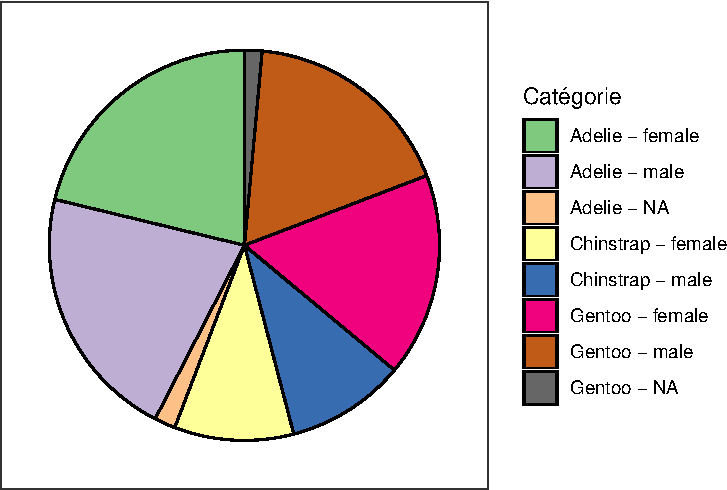
\includegraphics{03-Visualization_files/figure-pdf/fig-pie-1.pdf}

}

\caption{\label{fig-pie}Répartition des effectifs par espèce et par
sexe}

\end{figure}%

\begin{itemize}
\tightlist
\item
  Quelle est la catégorie la plus représentée ?
\item
  De combien de fois la part des Gentoo mâles est-elle supérieure à
  celle des Chinstrap femelles ? (1,5 fois, 2 fois, 2.5 fois ?\ldots)
\item
  Quelle est la quatrième catégorie la plus représentée ?
\end{itemize}

Il est difficile (voir impossible) de répondre précisément à ces
questions avec le diagramme circulaire de la Figure~\ref{fig-pie}, alors
qu'il est très simple d'obtenir des réponses précises avec un diagramme
bâtons tel que présenté à la Figure~\ref{fig-bpspecies-sex} ci-dessous
(vérifiez-le !) :

\begin{figure}

\centering{

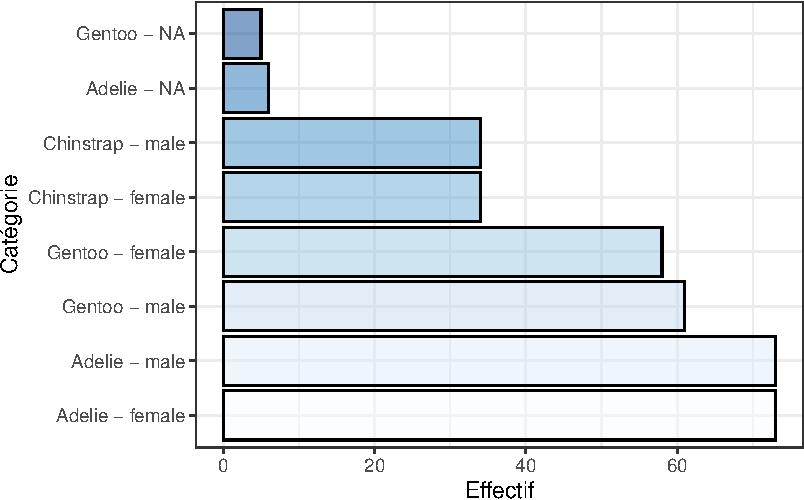
\includegraphics{03-Visualization_files/figure-pdf/fig-bpspecies-sex-1.pdf}

}

\caption{\label{fig-bpspecies-sex}Répartition des effectifs par espèce
et par sexe}

\end{figure}%

\section{Deux variables numériques}\label{sec-deuxnum}

La représentation graphique la plus adaptée à la visualisation des
relations entre deux variables numériques est aussi l'une des plus
simples : il s'agit des nuages de points que nous avons déjà évoqués.
Ici dépendant, puisque nous disposons de 2 variables numériques, nous
allons en associer une à l'axe des \texttt{x} et l'autre à l'axe des
\texttt{y}. Si l'on pressent que l'une des deux variables pourrait
``expliquer'' la seconde, ou être en partie responsable de ses
variations, on l'appelle \textbf{variable explicative} et on la placera
alors sur l'axe des \texttt{x}. L'autre variable, celle que l'on suppose
influencée par la première est appelée \textbf{variable expliquée}, et
sera associée à l'axe des \texttt{y}.

Les nuages de points de 2 variables numériques permettent donc de
visualiser les relations (supposées ou réelles) entre deux variables.

\subsection{Nuage de points}\label{nuage-de-points}

\subsubsection{Syntaxe élémentaire}\label{syntaxe-uxe9luxe9mentaire-1}

Prenons un exemple : nous souhaitons examiner les relations qui existent
entre la masse corporelle des individus et la longueur de leur nageoire.
Une relation allométrique simple suppose en effet que plus un individu
est grand et lourd, plus ses membres seront développés. La nature de la
relation allométrique peut toutefois être radicalement différente selon
les espèces. Pour l'instant, nous ne nous intéressons pas aux
éventuelles différences entre espèces et nous examinerons donc
l'ensemble des données, toutes espèces confondues.

\begin{Shaded}
\begin{Highlighting}[]
\FunctionTok{ggplot}\NormalTok{(penguins, }\FunctionTok{aes}\NormalTok{(}\AttributeTok{x =}\NormalTok{ body\_mass\_g, }\AttributeTok{y =}\NormalTok{ flipper\_length\_mm)) }\SpecialCharTok{+}
  \FunctionTok{geom\_point}\NormalTok{()}
\end{Highlighting}
\end{Shaded}

\begin{verbatim}
Warning: Removed 2 rows containing missing values or values outside the scale range
(`geom_point()`).
\end{verbatim}

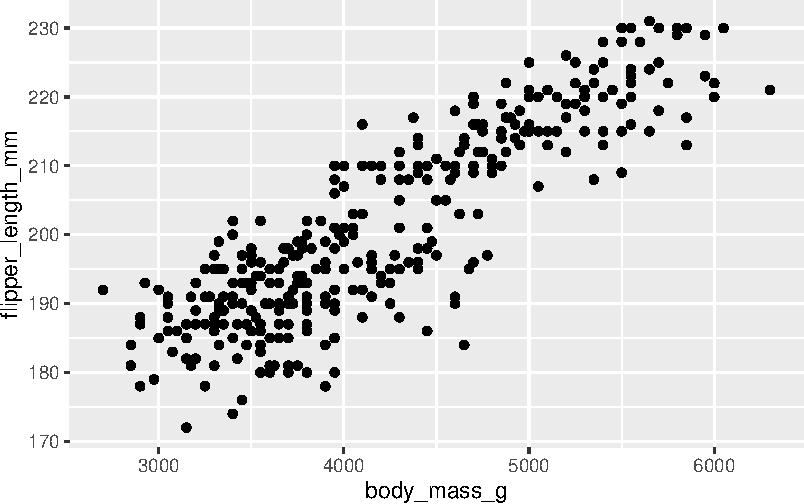
\includegraphics{03-Visualization_files/figure-pdf/unnamed-chunk-47-1.pdf}

Ici, j'associe \texttt{body\_mass\_g} à l'axe des \texttt{x} car je
suppose que c'est la variable explicative. Il est en effet plus logique
de considérer que la masse corporelle influence la longueur des
nageoires plutôt que le contraire. La variable expliquée, ici
\texttt{flipper\_length\_mm} est associée à l'axe des \texttt{y}.

La syntaxe est donc très simple, et le graphique obtenu permet de
constater que plus les individus sont lourds, plus leurs nageoires sont
longues.

\subsubsection{Droite de tendance}\label{droite-de-tendance}

Si l'on souhaite visualiser (modéliser !) cette association entre les
deux variables, on peut ajouter sur ce graphique une courbe de tendance
ou une droite de régression avec l'objet géométrique
\texttt{geom\_smooth()} :

\begin{Shaded}
\begin{Highlighting}[]
\FunctionTok{ggplot}\NormalTok{(penguins, }\FunctionTok{aes}\NormalTok{(}\AttributeTok{x =}\NormalTok{ body\_mass\_g, }\AttributeTok{y =}\NormalTok{ flipper\_length\_mm)) }\SpecialCharTok{+}
  \FunctionTok{geom\_point}\NormalTok{() }\SpecialCharTok{+}
  \FunctionTok{geom\_smooth}\NormalTok{(}\AttributeTok{method =} \StringTok{"lm"}\NormalTok{)}
\end{Highlighting}
\end{Shaded}

\begin{verbatim}
`geom_smooth()` using formula = 'y ~ x'
\end{verbatim}

\begin{verbatim}
Warning: Removed 2 rows containing non-finite outside the scale range
(`stat_smooth()`).
\end{verbatim}

\begin{verbatim}
Warning: Removed 2 rows containing missing values or values outside the scale range
(`geom_point()`).
\end{verbatim}

\includegraphics{03-Visualization_files/figure-pdf/unnamed-chunk-48-1.pdf}

L'argument \texttt{method\ =\ "lm"} indique que nous souhaitons ajouter
une droite de régression (\texttt{lm} est l'abréviation de ``linear
model''). L'intervalle grisé autour de la droite représente
l'incertitude associée à la régression et indique que la ``vraie''
droite de régression, dans la population générale (et pas seulement dans
notre échantillon de 344 individus) est probablement située dans cette
zone grisée. Nous aurons l'occasion de revenir en détail sur la notion
de régression linéaire et d'incertitude associée plus loin dans ce
livre.

\subsubsection{Autres caractéristiques
esthétiques}\label{autres-caractuxe9ristiques-esthuxe9tiques}

Comme pour tous les graphiques faisant apparaître des points, il est
possible de modifier les caractéristiques esthétiques habituelles, soit
en les associant à des variables du jeu de données (et en l'indiquant à
l'intérieur de \texttt{aes()}), soit en les fixant à des valeurs
constantes qui s'appliqueront à tous les points (et en l'indiquant alors
en dehors de \texttt{aes()}). L'exemple ci-dessous illustre ces
possibilités :

\begin{Shaded}
\begin{Highlighting}[]
\FunctionTok{ggplot}\NormalTok{(penguins, }\FunctionTok{aes}\NormalTok{(}\AttributeTok{x =}\NormalTok{ body\_mass\_g, }\AttributeTok{y =}\NormalTok{ flipper\_length\_mm, }\AttributeTok{fill =}\NormalTok{ species)) }\SpecialCharTok{+}
  \FunctionTok{geom\_point}\NormalTok{(}\AttributeTok{shape =} \DecValTok{21}\NormalTok{, }\AttributeTok{color =} \StringTok{"black"}\NormalTok{, }\AttributeTok{alpha =} \FloatTok{0.6}\NormalTok{) }\SpecialCharTok{+}
  \FunctionTok{geom\_smooth}\NormalTok{(}\FunctionTok{aes}\NormalTok{(}\AttributeTok{color =}\NormalTok{ species), }\AttributeTok{method =} \StringTok{"lm"}\NormalTok{, }\AttributeTok{se =} \ConstantTok{FALSE}\NormalTok{)}
\end{Highlighting}
\end{Shaded}

\begin{verbatim}
`geom_smooth()` using formula = 'y ~ x'
\end{verbatim}

\begin{verbatim}
Warning: Removed 2 rows containing non-finite outside the scale range
(`stat_smooth()`).
\end{verbatim}

\begin{verbatim}
Warning: Removed 2 rows containing missing values or values outside the scale range
(`geom_point()`).
\end{verbatim}

\includegraphics{03-Visualization_files/figure-pdf/unnamed-chunk-49-1.pdf}

L'argument \texttt{se\ =\ FALSE} de la fonction \texttt{geom\_smooth()}
permet de ne pas afficher l'intervalle d'incertitude de la régression
linéaire. Ici, j'ai associé la couleur de remplissage des points et la
couleur des droites de régression aux espèces (donc à l'intérieur de
\texttt{aes()}, soit dans \texttt{ggplot()} soit dans
\texttt{geom\_smooth()}), et j'ai fixé pour tous les points, le choix du
type de symbole (\texttt{shape\ =\ 21}, voir Figure~\ref{fig-pch}), la
couleur de contour (\texttt{color\ =\ "black"}) et la transparence
\texttt{alpha\ =\ 0.6}.

Là encore, il ne s'agit plus strictement d'un graphique représentant les
relations entre 2 variables numériques, mais bien entre 3 variables :
deux variables numériques (\texttt{body\_mass\_g} et
\texttt{flipper\_length\_mm}) et une variable catégorielle ou facteur
(\texttt{species}). Il est finalement très simple d'ajouter d'autres
variables sur un graphique bivarié tel qu'un nuage de points.

\subsection{Les graphiques en lignes}\label{les-graphiques-en-lignes}

Les graphiques en lignes, ou ``linegraphs'' sont généralement utilisés
lorsque l'axe des \texttt{x} porte une information \textbf{temporelle},
et l'axe des \texttt{y} une autre variable numérique. Le temps est une
variable naturellement ordonnée : les jours, semaines, mois, années, se
suivent naturellement. Les graphiques en lignes devraient être évités
lorsqu'il n'y a pas une organisation séquentielle évidente de la
variable portée par l'axe des \texttt{x}. Ainsi, lorsque l'une des 2
variables dont on dispose est une variable numérique temporelle (des
dates, des heures, etc.), on la place sur l'axe des \texttt{x} et la
seconde variable, dont on étudiera les fluctuations au cours du temps,
sur l'axe des \texttt{y}. On peut alors relier les valeurs grâce à
l'objet géométrique \texttt{geom\_line()} afin de créer une série
temporelle. Pour illustrer cela, examinons un autre jeu de données qui
contient une variable temporelle :

\begin{Shaded}
\begin{Highlighting}[]
\NormalTok{economics}
\end{Highlighting}
\end{Shaded}

\begin{verbatim}
# A tibble: 574 x 6
   date         pce    pop psavert uempmed unemploy
   <date>     <dbl>  <dbl>   <dbl>   <dbl>    <dbl>
 1 1967-07-01  507. 198712    12.6     4.5     2944
 2 1967-08-01  510. 198911    12.6     4.7     2945
 3 1967-09-01  516. 199113    11.9     4.6     2958
 4 1967-10-01  512. 199311    12.9     4.9     3143
 5 1967-11-01  517. 199498    12.8     4.7     3066
 6 1967-12-01  525. 199657    11.8     4.8     3018
 7 1968-01-01  531. 199808    11.7     5.1     2878
 8 1968-02-01  534. 199920    12.3     4.5     3001
 9 1968-03-01  544. 200056    11.7     4.1     2877
10 1968-04-01  544  200208    12.3     4.6     2709
# i 564 more rows
\end{verbatim}

Le jeu de données \texttt{economics} est fourni avec le package
\texttt{ggplot2}. Puisque vous avez chargé ce package (ou le
\texttt{tidyverse} qui contient ce package), vous devriez pouvoir
accéder à ce tableau sans difficulté. Nous nous intéresserons ici à la
variable \texttt{date} que nous placerons sur l'axe des \texttt{x} et à
la variable \texttt{uempmed} qui est la durée de chômage médiane dans la
population américaine, en nombre de semaines, que nous placerons sur
l'axe des \texttt{y}. Examinons donc comment la durée médiane du du
chômage a évolué au fil du temps :

\begin{Shaded}
\begin{Highlighting}[]
\FunctionTok{ggplot}\NormalTok{(economics, }\FunctionTok{aes}\NormalTok{(}\AttributeTok{x =}\NormalTok{ date, }\AttributeTok{y =}\NormalTok{ uempmed)) }\SpecialCharTok{+}
  \FunctionTok{geom\_line}\NormalTok{()}
\end{Highlighting}
\end{Shaded}

\includegraphics{03-Visualization_files/figure-pdf/unnamed-chunk-51-1.pdf}

Notez que puisque la variable \texttt{date} du tableau
\texttt{economics} est comprise par \texttt{R} comme étant du type
``variable temporelle'' (le type indiqué dans le tableau, juste sous le
nom de variable, est \texttt{\textless{}date\textgreater{}}), l'axe des
abscisses du graphique, qui est associé à cette variable, est
correctement mis en forme : seules les années apparaissent.

Les graphiques en lignes permettent de visualiser des
progressions/évolutions lorsqu'il existe une temporalité entre les
données. Sur l'exemple, traité plus haut, du lien entre masse et
longueur des nageoire des manchots, relier les points n'aurait
absolument aucun sens puisque toutes les observations sont indépendantes
: elles correspondent à des individus différents. Soyez donc prudents
lorsque vous reliez les points dur un graphique. Cela n'est possible que
lorsque les données le permettent. Vous devez donc toujours vous poser
la question de la pertinence de vos choix de représentations.

Comme pour les autres types de graphiques, il est possible de modifier
les caractéristiques esthétiques des lignes sur un graphique, en
particulier :

\begin{itemize}
\tightlist
\item
  \texttt{color} : la couleur des lignes
\item
  \texttt{size} : l'épaisseur des lignes
\item
  \texttt{linetype} : le type de ligne (continue, pointillée, tirets,
  etc. Essayez plusieurs valeurs entières pour comparer les types de
  lignes)
\end{itemize}

\begin{Shaded}
\begin{Highlighting}[]
\FunctionTok{ggplot}\NormalTok{(economics, }\FunctionTok{aes}\NormalTok{(}\AttributeTok{x =}\NormalTok{ date, }\AttributeTok{y =}\NormalTok{ uempmed)) }\SpecialCharTok{+}
  \FunctionTok{geom\_line}\NormalTok{(}\AttributeTok{color =} \StringTok{"orange"}\NormalTok{, }\AttributeTok{linetype =} \DecValTok{2}\NormalTok{)}
\end{Highlighting}
\end{Shaded}

\includegraphics{03-Visualization_files/figure-pdf/unnamed-chunk-52-1.pdf}

L'argument \texttt{linetype} est également utilisable par l'objet
géométrique \texttt{geom\_smooth()} :

\begin{Shaded}
\begin{Highlighting}[]
\FunctionTok{ggplot}\NormalTok{(economics, }\FunctionTok{aes}\NormalTok{(}\AttributeTok{x =}\NormalTok{ date, }\AttributeTok{y =}\NormalTok{ uempmed)) }\SpecialCharTok{+}
  \FunctionTok{geom\_line}\NormalTok{() }\SpecialCharTok{+}
  \FunctionTok{geom\_smooth}\NormalTok{(}\AttributeTok{se =} \ConstantTok{FALSE}\NormalTok{, }\AttributeTok{linetype =} \DecValTok{4}\NormalTok{, }\AttributeTok{color =} \StringTok{"red"}\NormalTok{)}
\end{Highlighting}
\end{Shaded}

\begin{verbatim}
`geom_smooth()` using method = 'loess' and formula = 'y ~ x'
\end{verbatim}

\includegraphics{03-Visualization_files/figure-pdf/unnamed-chunk-53-1.pdf}

Globalement, la durée médiane de chômage aux USA varie de façon
cyclique. La durée des cycles varie selon les période entre 5 et 10 ans
environ. Depuis les années 2000, la durée de chômage a augmenté de façon
très importante, pour passer de 5 à 6 semaines en 2001, à plus de 25
semaines en 2011.

\subsection{Les cartes}\label{les-cartes}

Les latitudes et longitudes sont un autre type de variable numériques
très particulières qui permettent notamment de produire des cartes. Il
s'agit ici d'un domaine extrêmement vaste qui dépasse largement le cadre
de ce livre. Retenez simplement qu'il est possible de produire des
cartes très informatives avec \texttt{ggplot2}, et quelques autres
packages spécialisés :

\includegraphics{images/map.png} En règle général, les cartes portent un
grand nombre de variables, numériques et/ou catégorielles. Mais tout
commence toujours par 2 variables numériques, les latitudes et longitude
des structures/informations que l'on souhaite représenter (traits de
côte, profiles bathymétriques, lieux d'observations diverses, \ldots).

\section{Deux variables
catégorielles}\label{deux-variables-catuxe9gorielles}

Lorsque l'on souhaite examiner les relations entre deux variables
catégorielles (ou facteurs), on a en général le choix entre les types de
représentations graphiques suivants :

\begin{itemize}
\tightlist
\item
  les diagrammes bâtons empilés
\item
  les diagrammes bâtons juxtaposés
\item
  les diagrammes bâtons ``facettés''
\item
  les graphiques en mosaïque (ou mosaic plots)
\end{itemize}

Pour toutes ces méthodes, des données qui n'ont pas été comptées au
préalable sont requises. Il est en effet beaucoup plus simple de
travailler avec le \texttt{tidyverse} (donc avec \texttt{ggplot2})
lorsque chaque ligne d'un tableau correspond à une observation plutôt
qu'à une somme d'observation. C'est le concept de \textbf{tableau
rangé}, central dans le traitement de données ainsi que pour
l'utilisation de tous les packages du \texttt{tidyverse}, et qui stipule
qu'un tableau de données devrait contenir une unique ligne pour chaque
observation, et une unique colonne pour chaque variable. Nous aurons
l'occasion (notamment en L3) de voir des tableaux qui ne respectent pas
ces règles et que nous devrons donc ré-organiser pour permettre leur
analyse et les représentations graphiques.

Nous allons passer ces différentes possibilités en revue pour examiner
les liens entre 2 variables catégorielles du jeu de données
\texttt{penguins} : \texttt{species} et \texttt{sex}. La première
renseigne sur l'espèce à laquelle un individu étudié appartient. La
seconde renseigne sur le sexe de chaque individu. L'étude du sex-ratio
est en effet souvent essentielle pour comprendre l'écologie des espèces.
Les sexe-ratios sont-ils équilibrés ou non. Et s'ils ne sont pas
équilibrés, sont-ils en faveur des mâles ou des femelles ?

\subsection{Diagrammes bâtons empilés}\label{sec-empil}

La façon la plus simple (mais rarement la meilleure) de procéder pour
visualiser 2 facteurs conjointement est de créer un diagramme bâtons
empilés :

\begin{Shaded}
\begin{Highlighting}[]
\FunctionTok{ggplot}\NormalTok{(penguins, }\FunctionTok{aes}\NormalTok{(}\AttributeTok{x =}\NormalTok{ species, }\AttributeTok{fill =}\NormalTok{ sex)) }\SpecialCharTok{+}
  \FunctionTok{geom\_bar}\NormalTok{()}
\end{Highlighting}
\end{Shaded}

\includegraphics{03-Visualization_files/figure-pdf/unnamed-chunk-54-1.pdf}

Ici, les espèces sont associées à l'axe des \texttt{x}
(\texttt{x\ =\ species}) et la couleur de remplissage des barres est
associée au sexe des individus (\texttt{fill\ =\ sex}), à l'intérieur de
la fonction \texttt{aes()}. Comme toujours, on peut modifier certaines
caractéristiques esthétiques (couleur de contour des barres,
transparence, etc.) et ré-ordonner les espèces sur l'axe des abscisses :

\begin{Shaded}
\begin{Highlighting}[]
\FunctionTok{ggplot}\NormalTok{(penguins, }\FunctionTok{aes}\NormalTok{(}\AttributeTok{x =} \FunctionTok{fct\_infreq}\NormalTok{(species), }\AttributeTok{fill =}\NormalTok{ sex)) }\SpecialCharTok{+}
  \FunctionTok{geom\_bar}\NormalTok{(}\AttributeTok{alpha =} \FloatTok{0.6}\NormalTok{, }\AttributeTok{color =} \StringTok{"black"}\NormalTok{)}
\end{Highlighting}
\end{Shaded}

\includegraphics{03-Visualization_files/figure-pdf/unnamed-chunk-55-1.pdf}

Ce type de visualisation est utile pour se rendre compte des ordres de
grandeur. On voit ici clairement que l'espèce Adélie est la plus
représentée dans cette étude, suivie par l'espèce Gentoo, et enfin
l'espèce Chinstrap. Pour chacune de ces 3 espèces, le sex-ratio a l'air
très équilibré. Toutefois, des différences subtiles de proportions entre
mâles et femelles selon les espèces pourraient être masqués par les
effectifs inégaux entre espèces. Il peut donc être préférable, pour
comparer des proportions, de normaliser les effectifs de toutes les
espèces pour ramener chaque barre du graphique à la même hauteur :

\begin{Shaded}
\begin{Highlighting}[]
\FunctionTok{ggplot}\NormalTok{(penguins, }\FunctionTok{aes}\NormalTok{(}\AttributeTok{x =} \FunctionTok{fct\_infreq}\NormalTok{(species), }\AttributeTok{fill =}\NormalTok{ sex)) }\SpecialCharTok{+}
  \FunctionTok{geom\_bar}\NormalTok{(}\AttributeTok{alpha =} \FloatTok{0.6}\NormalTok{, }\AttributeTok{color =} \StringTok{"black"}\NormalTok{, }\AttributeTok{position =} \StringTok{"fill"}\NormalTok{)}
\end{Highlighting}
\end{Shaded}

\includegraphics{03-Visualization_files/figure-pdf/unnamed-chunk-56-1.pdf}

L'argument \texttt{position\ =\ "fill"} de la fonction
\texttt{geom\_bar()} permet de transformer en proportions les abondances
de chaque modalités de la variable portée par l'axe des \texttt{x}.
L'axe des ordonnées varie maintenant entre 0 et 1 (0\% et 100\%), ce qui
rend les comparaisons plus aisées. Ici, le fait que le sexe de quelques
individus n'ait pas pu être déterminé vient gêner la lecture du
graphique. On peut supprimer ces valeurs grâce à la fonction
\texttt{filter()} du packages \texttt{dplyr}. Nous verrons dans le
\#sec-wrangling la signification du code suivant. Pour l'instant retenez
simplement qu'il permet d'éliminer les individus dont le sexe est
inconnu :

\begin{Shaded}
\begin{Highlighting}[]
\NormalTok{penguins }\SpecialCharTok{\%\textgreater{}\%} 
  \FunctionTok{filter}\NormalTok{(}\SpecialCharTok{!}\FunctionTok{is.na}\NormalTok{(sex)) }\SpecialCharTok{\%\textgreater{}\%} 
  \FunctionTok{ggplot}\NormalTok{(}\FunctionTok{aes}\NormalTok{(}\AttributeTok{x =} \FunctionTok{fct\_infreq}\NormalTok{(species), }\AttributeTok{fill =}\NormalTok{ sex)) }\SpecialCharTok{+}
  \FunctionTok{geom\_bar}\NormalTok{(}\AttributeTok{alpha =} \FloatTok{0.6}\NormalTok{, }\AttributeTok{color =} \StringTok{"black"}\NormalTok{, }\AttributeTok{position =} \StringTok{"fill"}\NormalTok{)}
\end{Highlighting}
\end{Shaded}

\includegraphics{03-Visualization_files/figure-pdf/unnamed-chunk-57-1.pdf}

On peut maintenant constater très facilement que le sex-ratio est
parfaitement équilibré pour les espèces Adélie et Chinstrap, et qu'il
est très légèrement en faveur des mâles pour l'espèce Gentoo.

\subsection{Diagrammes bâtons juxtaposés}\label{sec-juxta}

La syntaxe permettant de produire un diagramme bâtons juxtaposé est très
similaire à celle décrite ci-dessus :

\begin{Shaded}
\begin{Highlighting}[]
\FunctionTok{ggplot}\NormalTok{(penguins, }\FunctionTok{aes}\NormalTok{(}\AttributeTok{x =} \FunctionTok{fct\_infreq}\NormalTok{(species), }\AttributeTok{fill =}\NormalTok{ sex)) }\SpecialCharTok{+}
  \FunctionTok{geom\_bar}\NormalTok{(}\AttributeTok{alpha =} \FloatTok{0.6}\NormalTok{, }\AttributeTok{color =} \StringTok{"black"}\NormalTok{, }\AttributeTok{position =} \StringTok{"dodge"}\NormalTok{)}
\end{Highlighting}
\end{Shaded}

\includegraphics{03-Visualization_files/figure-pdf/unnamed-chunk-58-1.pdf}

La seule chose qui a changé est la valeur prise par l'argument
\texttt{position}, que l'on fixe ici à \texttt{dodge}. L'avantage de
cette représentation est qu'elle permet à la fois de visualiser les
effectifs de chaque catégorie et sous-catégorie (espèce et sexe), ainsi
que de comparer les proportions au sein de chaque espèce. Un
inconvénient et que lorsque les catégories n'ont pas toutes le même
nombre de sous-catégories, les barres ont des largeurs différentes. Ici,
l'espèce Chinstrap, qui n'a que 2 sous catégories (\texttt{female} et
\texttt{male}) présente des barres plus larges que les deux autres
espèces qui présentent chacune 3 sous-catégories (\texttt{female},
\texttt{male} et \texttt{NA}). Pour y remédier, on peut :

\begin{itemize}
\tightlist
\item
  soit retirer les données manquantes, comme précédemment :
\end{itemize}

\begin{Shaded}
\begin{Highlighting}[]
\NormalTok{penguins }\SpecialCharTok{\%\textgreater{}\%} 
  \FunctionTok{filter}\NormalTok{(}\SpecialCharTok{!}\FunctionTok{is.na}\NormalTok{(sex)) }\SpecialCharTok{\%\textgreater{}\%} 
  \FunctionTok{ggplot}\NormalTok{(}\FunctionTok{aes}\NormalTok{(}\AttributeTok{x =} \FunctionTok{fct\_infreq}\NormalTok{(species), }\AttributeTok{fill =}\NormalTok{ sex)) }\SpecialCharTok{+}
  \FunctionTok{geom\_bar}\NormalTok{(}\AttributeTok{alpha =} \FloatTok{0.6}\NormalTok{, }\AttributeTok{color =} \StringTok{"black"}\NormalTok{, }\AttributeTok{position =} \StringTok{"dodge"}\NormalTok{)}
\end{Highlighting}
\end{Shaded}

\includegraphics{03-Visualization_files/figure-pdf/unnamed-chunk-59-1.pdf}

\begin{itemize}
\tightlist
\item
  soit imposer que toutes les sous-catégories apparaissent pour chaque
  catégorie :
\end{itemize}

\begin{Shaded}
\begin{Highlighting}[]
\FunctionTok{ggplot}\NormalTok{(penguins, }\FunctionTok{aes}\NormalTok{(}\AttributeTok{x =} \FunctionTok{fct\_infreq}\NormalTok{(species), }\AttributeTok{fill =}\NormalTok{ sex)) }\SpecialCharTok{+}
  \FunctionTok{geom\_bar}\NormalTok{(}\AttributeTok{alpha =} \FloatTok{0.6}\NormalTok{, }\AttributeTok{color =} \StringTok{"black"}\NormalTok{,}
           \AttributeTok{position =} \FunctionTok{position\_dodge}\NormalTok{(}\AttributeTok{preserve =} \StringTok{"single"}\NormalTok{) )}
\end{Highlighting}
\end{Shaded}

\includegraphics{03-Visualization_files/figure-pdf/unnamed-chunk-60-1.pdf}

Ici, l'argument \texttt{position} prend une valeur plus complexe puisque
nous faisons appel à une fonction nommée \texttt{position\_dodge()}.
C'est l'argument \texttt{preserve\ =\ "single"} qui permet de s'assurer
que toutes les sous-catégories sont bien représentées au sein de chaque
catégorie, et donc, que toutes les barres ont bien la même largueur.

Le choix d'une méthode ou de l'autre dépend de ce que l'on souhaite
montrer : il n'y a pas une façon de faire meilleure ou moins bonne que
l'autre. Tout dépend de l'objectif poursuivi par l'auteur du graphique.

\subsection{Diagrammes bâtons ``facettés''}\label{sec-facet}

Dans le jargon de \texttt{ggplot2}, les \texttt{facet}s sont simplement
des sous-graphiques. Typiquement, une variable catégorielle peut être
utilisée pour représenter un sous-graphique pour chaque modalité de
cette variable. Ici, on peut par exemple produire un diagramme bâton
pour chaque espèce, et l'axe des \texttt{x} de chaque graphique portera
la variable \texttt{sex} :

\begin{Shaded}
\begin{Highlighting}[]
\FunctionTok{ggplot}\NormalTok{(penguins, }\FunctionTok{aes}\NormalTok{(}\AttributeTok{x =}\NormalTok{ sex)) }\SpecialCharTok{+}
  \FunctionTok{geom\_bar}\NormalTok{() }\SpecialCharTok{+}
  \FunctionTok{facet\_wrap}\NormalTok{(}\SpecialCharTok{\textasciitilde{}}\NormalTok{species)}
\end{Highlighting}
\end{Shaded}

\includegraphics{03-Visualization_files/figure-pdf/unnamed-chunk-61-1.pdf}

C'est la fonction \texttt{facet\_wrap()} qui permet de produire
plusieurs sous graphiques. Examinons quelques-une de ces particularités
:

\begin{itemize}
\tightlist
\item
  sa syntaxe fait appel à la notion de ``formule'', utilisée pour
  certaines fonctions spécifiques dans le langage \texttt{R}. Nous en
  verrons des exemples en L3 pour illustrer certains tests statistiques.
  Le tilde \texttt{\textasciitilde{}} se lit ``en fonction de''. Ici
  \texttt{\textasciitilde{}species} signifie ``crée des facets en
  fonction des espèces'', autrement dit, produit un sous-graphique par
  modalité de la variable \texttt{species}.
\item
  par défaut, les axes de tous les sous graphiques sont strictement
  identiques, en abscisse comme en ordonnée. On peut modifier ce
  comportement grâce à l'un des arguments suivants :
  \texttt{scales\ =\ "free\_x"} (pour que les axes des abscisses soient
  indépendants entre les sous-graphiques), \texttt{scales\ =\ "free\_y"}
  (pour que les axes des ordonnées soient indépendants entre les
  sous-graphiques) ou \texttt{scales\ =\ "free"} (pour quelles deux axes
  soient indépendants entre les sous-graphiques)
\item
  l'argument \texttt{ncol\ =} permet de spécifier le nombre de colonnes
  souhaité pour l'organisation des sous-graphiques
\end{itemize}

Voici un exemple de ces syntaxes :

\begin{Shaded}
\begin{Highlighting}[]
\FunctionTok{ggplot}\NormalTok{(penguins, }\FunctionTok{aes}\NormalTok{(}\AttributeTok{x =}\NormalTok{ sex)) }\SpecialCharTok{+}
  \FunctionTok{geom\_bar}\NormalTok{() }\SpecialCharTok{+}
  \FunctionTok{facet\_wrap}\NormalTok{(}\SpecialCharTok{\textasciitilde{}}\NormalTok{species, }\AttributeTok{scales =} \StringTok{"free\_y"}\NormalTok{, }\AttributeTok{ncol =} \DecValTok{2}\NormalTok{)}
\end{Highlighting}
\end{Shaded}

\includegraphics{03-Visualization_files/figure-pdf/unnamed-chunk-62-1.pdf}

Les 3 sous-graphiques sont maintenant disposés dans 2 colonnes, et si
l'axe des \texttt{x} est toujours le même pour chaque sous-graphique,
les axes des \texttt{y} sont différents pour les 3 sous-graphiques.

Pour égayer un peu ce graphique, ajoutons une couleur de remplissage
pour les barres, selon l'espèce :

\begin{Shaded}
\begin{Highlighting}[]
\FunctionTok{ggplot}\NormalTok{(penguins, }\FunctionTok{aes}\NormalTok{(}\AttributeTok{x =}\NormalTok{ sex, }\AttributeTok{fill =}\NormalTok{ species)) }\SpecialCharTok{+}
  \FunctionTok{geom\_bar}\NormalTok{(}\AttributeTok{color =} \StringTok{"black"}\NormalTok{, }\AttributeTok{alpha =} \FloatTok{0.7}\NormalTok{) }\SpecialCharTok{+}
  \FunctionTok{facet\_wrap}\NormalTok{(}\SpecialCharTok{\textasciitilde{}}\NormalTok{species, }\AttributeTok{scales =} \StringTok{"free\_y"}\NormalTok{, }\AttributeTok{ncol =} \DecValTok{2}\NormalTok{)}
\end{Highlighting}
\end{Shaded}

\includegraphics{03-Visualization_files/figure-pdf/unnamed-chunk-63-1.pdf}

La légende qui est automatiquement créée à droite est inutile puisque
les sous-graphiques indiquent déjà le nom des espèces. Pour retirer une
légende inutile, on peut utiliser l'argument
\texttt{show.legend\ =\ FALSE} de la plupart des objets géométriques :

\begin{Shaded}
\begin{Highlighting}[]
\FunctionTok{ggplot}\NormalTok{(penguins, }\FunctionTok{aes}\NormalTok{(}\AttributeTok{x =}\NormalTok{ sex, }\AttributeTok{fill =}\NormalTok{ species)) }\SpecialCharTok{+}
  \FunctionTok{geom\_bar}\NormalTok{(}\AttributeTok{color =} \StringTok{"black"}\NormalTok{, }\AttributeTok{alpha =} \FloatTok{0.7}\NormalTok{, }\AttributeTok{show.legend =} \ConstantTok{FALSE}\NormalTok{) }\SpecialCharTok{+}
  \FunctionTok{facet\_wrap}\NormalTok{(}\SpecialCharTok{\textasciitilde{}}\NormalTok{species, }\AttributeTok{scales =} \StringTok{"free\_y"}\NormalTok{, }\AttributeTok{ncol =} \DecValTok{2}\NormalTok{)}
\end{Highlighting}
\end{Shaded}

\includegraphics{03-Visualization_files/figure-pdf/unnamed-chunk-64-1.pdf}

\subsection{Mosaïc plots}\label{sec-mosa}

Les graphiques en mosaïque sont une alternative aux diagrammes bâtons en
tous genre. Ils permettent de visualiser à la fois les effectifs et de
comparer les proportions. La difficulté de ce genre de graphique est
qu'il n'existe pas d'objet géométrique permettant de les représenter
simplement dans le package \texttt{ggplot2}. Le package
\texttt{ggmosaic} de Jeppson, Hofmann, et Cook (2021) est toutefois
entièrement dédié à ce type de graphique. Installez ce package puis
chargez-le en mémoire :

\begin{Shaded}
\begin{Highlighting}[]
\FunctionTok{install.packages}\NormalTok{(}\StringTok{"ggmosaic"}\NormalTok{)}
\FunctionTok{library}\NormalTok{(ggmosaic)}
\end{Highlighting}
\end{Shaded}

On peut maintenant accéder à un nouvel objet géométrique,
\texttt{geom\_mosaic()}, dont l'utilisation est un peu différente de
celle que nous avons vu jusqu'ici :

\begin{Shaded}
\begin{Highlighting}[]
\FunctionTok{ggplot}\NormalTok{(penguins) }\SpecialCharTok{+}
  \FunctionTok{geom\_mosaic}\NormalTok{(}\FunctionTok{aes}\NormalTok{(}\AttributeTok{x =} \FunctionTok{product}\NormalTok{(species), }\AttributeTok{fill =}\NormalTok{ sex))}
\end{Highlighting}
\end{Shaded}

\includegraphics{03-Visualization_files/figure-pdf/unnamed-chunk-67-1.pdf}

Il faut obligatoirement :

\begin{enumerate}
\def\labelenumi{\arabic{enumi}.}
\tightlist
\item
  spécifier \texttt{aes()} à l'intérieur de \texttt{geom\_mosaic()} et
  non à l'intérieur de \texttt{ggplot()}
\item
  utiliser la fonction \texttt{product()} (qui fait elle aussi partie du
  package \texttt{ggmosaic}) pour indiquer quelle variable catégorielle
  on souhaite associer à l'axe des \texttt{x}
\item
  Comme pour les diagrammes bâtons, la couleur de remplissage est
  associée à la seconde variable catégorielle de façon tout à fait
  classique
\end{enumerate}

Comme pour les diagrammes en bâtons empilés pour lesquels on spécifie
\texttt{position\ =\ "fill"}, toutes les barres d'un graphique en
mosaïque ont la même hauteur, ce qui permet de visualiser les
proportions de chaque sexe pour chaque espèce, mais pas les effectifs.
C'est ici la largueur des barres qui est proportionnelle aux effectifs
de chaque espèce. Si on n'accède par directement aux valeurs absolues,
on peut néanmoins effectuer des comparaisons d'ordres de grandeur.
L'espèce Adélie est ainsi la plus représentée dans nos données, suivie
de l'espèce Gentoo puis de l'espèce Chinstrap.

Au final, le choix d'un graphique doit vous permettre de mettre en
évidence les relations qui vous paraissent importantes de la façon la
plus visuelle et évidente possible pour une personne ne connaissant pas
vos données. Votre choix dépendra donc des données disponibles et de
votre objectif (p.~ex. comparaisons de proportions ou de valeurs
absolues, nombreuses modalités ou seulement quelques unes, etc.).

\section{Une variable de chaque type}\label{sec-oneeach}

Les représentations graphiques réalisables et pertinentes lorsque l'on
dispose d'une variable numérique et d'un facteur sont souvent des
adaptations des graphiques précédents. Globalement, trois choix
s'offrent à nous :

\begin{enumerate}
\def\labelenumi{\arabic{enumi}.}
\tightlist
\item
  les histogrammes facettés
\item
  les stripcharts
\item
  les boîtes à moustaches. Nous donnerons ici un simple. La
  signification de tous les éléments de ces graphiques sera fournie à la
  Section~\ref{sec-reframe}
\end{enumerate}

Pour illustrer ces différentes possibilités, intéressons nous maintenant
à la relation qui existe entre l'épaisseur du bec des manchots
(\texttt{bill\_depth\_mm}, variable numérique) et l'espèce
(\texttt{species}, variable catégorielle ou facteur)

\subsection{Histogrammes ``facettés''}\label{sec-factorhisto}

La syntaxe est ici tout à fait classique. Pour réaliser un histogramme,
on place la variable numérique sur l'axe des abscisses. La variable
catégorielle nous servira à créer les sous graphiques, ici, un par
espèce. Afin de faciliter les comparaisons, nous placerons les
sous-graphiques les uns sous les autres en spécifiant
\texttt{ncol\ =\ 1}. Enfin, l'aspect général sera amélioré en modifiant
quelques caractéristiques esthétiques :

\begin{Shaded}
\begin{Highlighting}[]
\FunctionTok{ggplot}\NormalTok{(penguins, }\FunctionTok{aes}\NormalTok{(}\AttributeTok{x =}\NormalTok{ bill\_depth\_mm)) }\SpecialCharTok{+}
  \FunctionTok{geom\_histogram}\NormalTok{(}\AttributeTok{fill =} \StringTok{"steelblue"}\NormalTok{, }\AttributeTok{color =} \StringTok{"black"}\NormalTok{, }
                 \AttributeTok{alpha =} \FloatTok{0.6}\NormalTok{, }\AttributeTok{bins =} \DecValTok{20}\NormalTok{) }\SpecialCharTok{+}
  \FunctionTok{facet\_wrap}\NormalTok{(}\SpecialCharTok{\textasciitilde{}}\NormalTok{species, }\AttributeTok{ncol =} \DecValTok{1}\NormalTok{)}
\end{Highlighting}
\end{Shaded}

\begin{verbatim}
Warning: Removed 2 rows containing non-finite outside the scale range
(`stat_bin()`).
\end{verbatim}

\includegraphics{03-Visualization_files/figure-pdf/unnamed-chunk-68-1.pdf}

On peut aussi choisir d'utiliser une couleur pour chaque espèce (mais on
n'affichera pas la légende puisque les espèces sont déjà séparées dans
les sous graphiques). En outre, puisque les effectifs des Chinstrap sont
bien plus faibles que pour les deux autres espèces, on a intérêt à
``libérer'' l'axe des \texttt{y} afin que l'histogramme des Chinstrap
soit plus facilement lisible (il apparaît pour l'instant très ``écrasé''
comparé aux autres).

\begin{Shaded}
\begin{Highlighting}[]
\FunctionTok{ggplot}\NormalTok{(penguins, }\FunctionTok{aes}\NormalTok{(}\AttributeTok{x =}\NormalTok{ bill\_depth\_mm, }\AttributeTok{fill =}\NormalTok{ species)) }\SpecialCharTok{+}
  \FunctionTok{geom\_histogram}\NormalTok{(}\AttributeTok{show.legend =} \ConstantTok{FALSE}\NormalTok{, }\AttributeTok{color =} \StringTok{"black"}\NormalTok{, }
                 \AttributeTok{alpha =} \FloatTok{0.6}\NormalTok{, }\AttributeTok{bins =} \DecValTok{20}\NormalTok{) }\SpecialCharTok{+}
  \FunctionTok{facet\_wrap}\NormalTok{(}\SpecialCharTok{\textasciitilde{}}\NormalTok{species, }\AttributeTok{ncol =} \DecValTok{1}\NormalTok{, }\AttributeTok{scales =} \StringTok{"free\_y"}\NormalTok{)}
\end{Highlighting}
\end{Shaded}

\begin{verbatim}
Warning: Removed 2 rows containing non-finite outside the scale range
(`stat_bin()`).
\end{verbatim}

\includegraphics{03-Visualization_files/figure-pdf/unnamed-chunk-69-1.pdf}

Les Gentoo, qui ont pourtant des masses corporelles supérieures à celle
des deux autres espèces (voir Figure~\ref{fig-cloud} de la
Section~\ref{sec-cloud}), ont visiblement des becs moins épais (entre 12
et 17 mm) que les deux autres espèces (entre 16 et 22 mm).

\begin{tcolorbox}[enhanced jigsaw, colbacktitle=quarto-callout-important-color!10!white, colframe=quarto-callout-important-color-frame, bottomtitle=1mm, opacityback=0, arc=.35mm, leftrule=.75mm, titlerule=0mm, colback=white, title=\textcolor{quarto-callout-important-color}{\faExclamation}\hspace{0.5em}{Important}, toptitle=1mm, breakable, coltitle=black, rightrule=.15mm, left=2mm, opacitybacktitle=0.6, toprule=.15mm, bottomrule=.15mm]

C'est la position des données le long de l'axe des \texttt{x} qui nous
permet de faire des comparaisons pertinentes. Il est donc essentiel de
présenter les différents histogrammes les uns sous les autres, en
conservant la même échelle pour les abscisses de tous les
sous-graphiques.

\end{tcolorbox}

Ici, on peut donc discuter de la distribution de la variable numérique
pour chaque modalité de la variable catégorielle (\emph{i.e.} quelle
distribution de l'épaisseur des becs pour chaque espèce), mais on peut
en plus faire des comparaisons entre modalités (entre les espèces). Cela
est beaucoup plus pertinent que de s'intéresser à la distribution de
l'épaisseur des becs toutes espèces confondues.

\subsection{Les stripcharts}\label{sec-factorstrip}

Nous avons déjà abordé ce type de graphique dans la
Section~\ref{sec-cloud}. Contrairement à la situation où nous n'avions
qu'une variable numérique et où nous devions fixer \texttt{x\ =\ ""}
pour que toutes les observations se placent au même niveau de l'axe des
abscisses (voir Figure~\ref{fig-strip}), nous allons ici associer la
variable catégorielle à l'axe des \texttt{x}. La variable numérique sera
quant-à-elle toujours associée à l'axe des ordonnées :

\begin{Shaded}
\begin{Highlighting}[]
\FunctionTok{ggplot}\NormalTok{(penguins, }\FunctionTok{aes}\NormalTok{(}\AttributeTok{x =}\NormalTok{ species, }\AttributeTok{y =}\NormalTok{ bill\_depth\_mm)) }\SpecialCharTok{+}
  \FunctionTok{geom\_jitter}\NormalTok{(}\AttributeTok{width =} \FloatTok{0.20}\NormalTok{, }\AttributeTok{height =} \DecValTok{0}\NormalTok{)}
\end{Highlighting}
\end{Shaded}

\begin{verbatim}
Warning: Removed 2 rows containing missing values or values outside the scale range
(`geom_point()`).
\end{verbatim}

\begin{figure}[H]

\centering{

\includegraphics{03-Visualization_files/figure-pdf/fig-facstrip-1.pdf}

}

\caption{\label{fig-facstrip}Un exemple de stripchart}

\end{figure}%

Notez que la position des points sur l'axe des \texttt{y} doit
parfaitement correspondre aux valeurs contenues dans le jeu de données
pour la variable numérique d'intérêt. Cela signifie que l'argument
\texttt{height} doit obligatoirement être fixé à 0.

Comme pour les diagrammes bâtons, il est possible de produire des
stripcharts horizontaux. Les modifications à apporter sont alors les
suivantes :

\begin{itemize}
\tightlist
\item
  la variable numérique est associée à l'axe des \texttt{x}
\item
  la variable catégorielle est associée à l'axe des \texttt{y}
\item
  la dispersion horizontale \texttt{width} doit obligatoirement être
  fixée à 0
\item
  la dispersion verticale \texttt{height} doit être comprise entre 0.1
  et 0.4 pour étaler les points de chaque modalité et ainsi éviter
  l'overplotting
\end{itemize}

\begin{Shaded}
\begin{Highlighting}[]
\FunctionTok{ggplot}\NormalTok{(penguins, }\FunctionTok{aes}\NormalTok{(}\AttributeTok{x =}\NormalTok{ bill\_depth\_mm, }\AttributeTok{y =}\NormalTok{ species)) }\SpecialCharTok{+}
  \FunctionTok{geom\_jitter}\NormalTok{(}\AttributeTok{width =} \DecValTok{0}\NormalTok{, }\AttributeTok{height =} \FloatTok{0.20}\NormalTok{, }\AttributeTok{alpha =} \FloatTok{0.6}\NormalTok{)}
\end{Highlighting}
\end{Shaded}

\begin{verbatim}
Warning: Removed 2 rows containing missing values or values outside the scale range
(`geom_point()`).
\end{verbatim}

\includegraphics{03-Visualization_files/figure-pdf/unnamed-chunk-71-1.pdf}

\subsection{Les boîtes à moustaches ou boxplots}\label{sec-boxplot}

Voilà à quoi ressemble un graphique de ce type pour les données qui nous
intéressent (épaisseur des becs selon l'espèce) :

\begin{Shaded}
\begin{Highlighting}[]
\FunctionTok{ggplot}\NormalTok{(penguins, }\FunctionTok{aes}\NormalTok{(}\AttributeTok{x =}\NormalTok{ species, }\AttributeTok{y =}\NormalTok{ bill\_depth\_mm)) }\SpecialCharTok{+}
  \FunctionTok{geom\_boxplot}\NormalTok{()}
\end{Highlighting}
\end{Shaded}

\begin{verbatim}
Warning: Removed 2 rows containing non-finite outside the scale range
(`stat_boxplot()`).
\end{verbatim}

\includegraphics{03-Visualization_files/figure-pdf/unnamed-chunk-72-1.pdf}

Dans la forme, ça ressemble un à un stripchart (comparez par exemple
avec la syntaxe et les résultats obtenus à la
Figure~\ref{fig-facstrip}). Néanmoins, ici, au lieu de visualiser tous
les points du jeu de données, seules quelques valeurs caractéristiques
sont utilisées pour construire le boîte à moustache de chaque espèce.
Les différents éléments d'un boxplot, sont les suivants :

\begin{itemize}
\tightlist
\item
  La limite inférieure de la boîte correspond au premier quartile : 25\%
  des données de l'échantillon sont situées au-dessous de cette valeur.
\item
  La limite supérieure de la boîte correspond au troisième quartile :
  25\% des données de l'échantillon sont situées au-dessus de cette
  valeur.
\item
  Le segment épais à l'intérieur de la boîte correspond au second
  quartile : c'est la médiane de l'échantillon. 50\% des données de
  l'échantillon sont situées au-dessus de cette valeur, et 50\%
  au-dessous.
\item
  La hauteur de la boîte correspond à ce que l'on appelle l'étendue
  inter-quartile ou Inter Quartile Range (IQR) en anglais. On trouve
  dans cette boîte 50\% des observations de l'échantillon. C'est une
  mesure de la dispersion des 50\% des données les plus centrales. Une
  boîte plus allongée indique donc une plus grande dispersion.
\item
  Les moustaches correspondent à des valeurs qui sont en dessous du
  premier quartile (pour la moustache du bas) et au-dessus du troisième
  quartile (pour la moustache du haut). La règle utilisée dans
  \texttt{R} est que ces moustaches s'étendent jusqu'aux valeurs
  minimales et maximales de l'échantillon, mais elles ne peuvent en
  aucun cas s'étendre au-delà de 1,5 fois la hauteur de la boîte (1,5
  fois l'IQR) vers le haut et le bas. Si des points apparaissent au-delà
  des moustaches (vers le haut ou le bas), ces points sont appelés
  ``outliers''. On peut en observer un pour l'espèce Adélie. Ce sont des
  points qui s'éloignent du centre de la distribution de façon
  importante puisqu'ils sont au-delà de 1,5 fois l'IQR de part et
  d'autre du premier ou du troisième quartile. Il peut s'agir
  d'anomalies de mesures, d'anomalies de saisie des données, ou tout
  simplement, d'enregistrements tout à fait valides mais atypiques ou
  extrêmes. J'attire votre attention sur le fait que la définition de
  ces outliers est relativement arbitraire. Nous pourrions faire le
  choix d'étendre les moustaches jusqu'à 1,8 fois l'IQR (ou 2, ou 2,5).
  Nous observerions alors beaucoup moins d'outliers. D'une façons
  générale, la longueur des moustaches renseigne sur la variabilité des
  données en dehors de la zone centrale. Plus elles sont longues, plus
  la variabilité est importante. Et dans tous les cas, l'examen attentif
  des outliers est utile car il nous permet d'en apprendre plus sur le
  comportement extrême de certaines observations.
\end{itemize}

Lorsque les boîtes ont une forme à peu près symétrique de part et
d'autre de la médiane (c'est le cas pour notre exemple), cela signifie
qu'un histogramme des mêmes données serait symétrique également (on peut
le vérifier avec les histogrammes de la Section~\ref{sec-factorhisto}).

\subsubsection{L'intervalle de confiance à 95\% de la
médiane}\label{lintervalle-de-confiance-uxe0-95-de-la-muxe9diane}

On peut également ajouter une encoche autour de la valeur de médiane en
ajoutant l'argument \texttt{notch\ =\ TRUE} à la fonction
\texttt{geom\_boxplot()} :

\begin{Shaded}
\begin{Highlighting}[]
\FunctionTok{ggplot}\NormalTok{(penguins, }\FunctionTok{aes}\NormalTok{(}\AttributeTok{x =}\NormalTok{ species, }\AttributeTok{y =}\NormalTok{ bill\_depth\_mm)) }\SpecialCharTok{+}
  \FunctionTok{geom\_boxplot}\NormalTok{(}\AttributeTok{notch =} \ConstantTok{TRUE}\NormalTok{)}
\end{Highlighting}
\end{Shaded}

\begin{verbatim}
Warning: Removed 2 rows containing non-finite outside the scale range
(`stat_boxplot()`).
\end{verbatim}

\includegraphics{03-Visualization_files/figure-pdf/unnamed-chunk-73-1.pdf}

L'encoche qui apparaît sur chaque boîte à moustache correspond à
l'étendue de l'intervalle de confiance à 95\% de la médiane. Pour chaque
échantillon, nous espérons que la médiane calculée soit le reflet fidèle
de la vraie valeur de médiane de la population générale. Mais il sera
toujours impossible d'en avoir la certitude absolue. Le mieux que l'on
puisse faire, c'est quantifier l'incertitude associée à l'estimation de
la médiane à partir des données d'un échantillon. L'intervalle de
confiance nous indique qu'il y a de bonnes chances que la vraie valeur
de médiane de la population générale (qui restera à jamais inconnue) se
trouve dans cet intervalle.

Nous reviendrons sur cette notion importante plus tard dans le cursus,
car ce type de graphique nous permettra d'anticiper sur les résultats
des tests statistiques de comparaison de moyennes.

Au final, nous avons 3 moyens d'obtenir des informations de distribution
:

\begin{itemize}
\tightlist
\item
  observer l'ensemble des données brutes grâce à un nuage de points ou
  stripchart
\item
  regrouper en partie les données brutes dans les classes d'un
  histogramme. On ne visualise plus l'ensemble des données
  individuelles, mais un résumé de ces données puisqu'on ne dispose plus
  que d'une unique valeur pour chaque classe de l'histogramme.
  L'histogramme peut donc résumer des centaines voire des milliers de
  points sous la forme d'un petit nombre de classes (entre 10 et 40 en
  général)
\item
  regrouper très fortement les données brutes sous la forme d'une boîte
  à moustache. Les boîtes à moustaches permettent de résumer
  l'information de centaines ou milliers de points sous la forme d'un
  résumé statistique composé de 5 valeurs (minimum et maximum, médiane,
  premier et troisième quartiles), ou 7 si l'on ajoute les encoches des
  intervalles de confiance à 95\% des médianes. On observe alors moins
  facilement les nuances subtiles de distribution qu'avec un histogramme
  ou les données brutes, mais l'avantage est qu'on peut comparer
  facilement les grandes tendances d'un grand nombre de séries de
  données (parfois plusieurs dizaines) en plaçant des boîtes à
  moustaches côte à côte.
\end{itemize}

La Figure~\ref{fig-comboxplot} illustre ces 3 possibilités de
visualisation de la distribution d'une variable numérique (ici, la
distribution des masses corporelles des manchots Adélie) :

\begin{figure}

\centering{

\includegraphics{03-Visualization_files/figure-pdf/fig-comboxplot-1.pdf}

}

\caption{\label{fig-comboxplot}Trois façons de visualiser la
distribution des masses des manchots Adélie}

\end{figure}%

\section{Trois variables (et plus !)}\label{trois-variables-et-plus}

Lorsque l'on dispose de 3 variables, les situations possibles commencent
à être nombreuses :

\begin{itemize}
\tightlist
\item
  trois variables numériques
\item
  deux variables numériques et un facteur
\item
  une variable numérique et deux facteurs
\item
  trois facteurs
\end{itemize}

Pour chacune de ces situations, on peut en générale reprendre les types
de graphiques proposés dans les 3 sections précédentes consacrées aux
situations où l'on dispose de 2 variables (), et :

\begin{itemize}
\tightlist
\item
  soit ajouter une variable sous forme de code couleur (avec
  \texttt{color} ou \texttt{fill} à l'intérieur de \texttt{aes()})
\item
  soit ajouter une variable sous forme de \texttt{facets} (avec
  \texttt{facet\_wrap()} ou avec \texttt{facet\_grid()})
\end{itemize}

Les possibilités sont très nombreuses et il ne sera pas possible d'être
exhaustif ici. Je fournis néanmoins quelques exemples ci-dessous afin
que vous compreniez bien la logique. Ensuite, ça sera à vous
d'expérimenter selon les données dont vous disposez, les questions
scientifiques que vous vous posez, et les relations que vous souhaitez
explorer/visualiser.

\subsection{Trois variables
numériques}\label{trois-variables-numuxe9riques}

Dans cette situation, on fait en général un nuage de points qui porte
une variable numérique sur chaque axe, et on associe la troisième
variable numérique soit à la couleur des points, soit à leur taille
(soit aux deux à la fois). Par exemple, pour examiner les relations
entre longueur du bec, épaisseur du bec, et masse corporelle, on peut
procéder ainsi :

\begin{Shaded}
\begin{Highlighting}[]
\FunctionTok{ggplot}\NormalTok{(penguins, }\FunctionTok{aes}\NormalTok{(}\AttributeTok{x =}\NormalTok{ bill\_length\_mm, }\AttributeTok{y =}\NormalTok{ bill\_depth\_mm,}
                     \AttributeTok{size =}\NormalTok{ body\_mass\_g)) }\SpecialCharTok{+}
  \FunctionTok{geom\_point}\NormalTok{(}\AttributeTok{shape =} \DecValTok{21}\NormalTok{, }\AttributeTok{fill =} \StringTok{"steelblue"}\NormalTok{, }\AttributeTok{color =} \StringTok{"black"}\NormalTok{, }\AttributeTok{alpha =} \FloatTok{0.6}\NormalTok{)}
\end{Highlighting}
\end{Shaded}

\begin{verbatim}
Warning: Removed 2 rows containing missing values or values outside the scale range
(`geom_point()`).
\end{verbatim}

\includegraphics{03-Visualization_files/figure-pdf/unnamed-chunk-75-1.pdf}

C'est ce qu'on appelle un ``bubble plot''. Ici on constate que les
individus qui ont les becs les plus courts, sont aussi ceux qui ont un
bec épais (groupe de points en haut à gauche). Ces individus sont parmi
les plus légers (symboles de petite taille). À l'inverse, les individus
ayant les becs les plus longs ont aussi des becs peu épais (groupes de
points situés en bas à droite). Ces individus sont parmi les plus lourds
du jeu de données (symboles de grandes taille).

Une autre façon de visualiser ces mêmes données consiste à associer la
masse des individus à la couleur de remplissage des symboles :

\begin{Shaded}
\begin{Highlighting}[]
\FunctionTok{ggplot}\NormalTok{(penguins, }\FunctionTok{aes}\NormalTok{(}\AttributeTok{x =}\NormalTok{ bill\_length\_mm, }\AttributeTok{y =}\NormalTok{ bill\_depth\_mm,}
                     \AttributeTok{fill =}\NormalTok{ body\_mass\_g)) }\SpecialCharTok{+}
  \FunctionTok{geom\_point}\NormalTok{(}\AttributeTok{shape =} \DecValTok{21}\NormalTok{, }\AttributeTok{color =} \StringTok{"black"}\NormalTok{, }\AttributeTok{alpha =} \FloatTok{0.6}\NormalTok{, }\AttributeTok{size =} \DecValTok{2}\NormalTok{)}
\end{Highlighting}
\end{Shaded}

\begin{verbatim}
Warning: Removed 2 rows containing missing values or values outside the scale range
(`geom_point()`).
\end{verbatim}

\includegraphics{03-Visualization_files/figure-pdf/unnamed-chunk-76-1.pdf}

Cette fois, les individus les plus légers apparaissent en bleu très
sombre, et les individus les plus lourds en bleu très clair. Ce choix de
couleur nous est imposé, mais nous verrons plus loin comment le modifier
pour rendre ce type de graphique plus facile à lire. Lorsque nous
associons une variable numérique continue à la couleur des points, la
légende qui est générée automatiquement pour nous par \texttt{R} sera
toujours un gradient de couleurs. Si vous revenez en arrière au niveau
des graphiques en mosaïques (Section~\ref{sec-mosa}), ou au niveau des
diagrammes bâtons juxtaposés (Section~\ref{sec-juxta}), vous verrez que
lorsque la couleur est associée à une variable catégorielle (ou
facteur), la légende présente des couleurs distinctes, une pour chaque
modalité du facteur considéré. Là encore, \texttt{R} choisit les
couleurs pour nous. Mais là encore, nous verrons comment imposer des
couleurs différentes si les choix par défaut ne nous conviennent pas.

Enfin, il est évidemment possible de jouer à la fois sur la couleur et
sur la taille des symboles :

\begin{Shaded}
\begin{Highlighting}[]
\FunctionTok{ggplot}\NormalTok{(penguins, }\FunctionTok{aes}\NormalTok{(}\AttributeTok{x =}\NormalTok{ bill\_length\_mm, }\AttributeTok{y =}\NormalTok{ bill\_depth\_mm,}
                     \AttributeTok{fill =}\NormalTok{ body\_mass\_g, }\AttributeTok{size =}\NormalTok{ body\_mass\_g)) }\SpecialCharTok{+}
  \FunctionTok{geom\_point}\NormalTok{(}\AttributeTok{shape =} \DecValTok{21}\NormalTok{, }\AttributeTok{color =} \StringTok{"black"}\NormalTok{, }\AttributeTok{alpha =} \FloatTok{0.6}\NormalTok{)}
\end{Highlighting}
\end{Shaded}

\begin{verbatim}
Warning: Removed 2 rows containing missing values or values outside the scale range
(`geom_point()`).
\end{verbatim}

\includegraphics{03-Visualization_files/figure-pdf/unnamed-chunk-77-1.pdf}

Ici, l'information de masse est donc associée à 2 caractéristiques
esthétiques distinctes : la couleur de remplissage des points et leur
taille. Cela rend la lecture plus facile dans certaines situations.

Au final, nous avons donc associé 3 variables numériques à 4
caractéristiques esthétiques du graphique :

\begin{itemize}
\tightlist
\item
  \texttt{bill\_length\_mm} est associée à \texttt{x}
\item
  \texttt{bill\_depth\_mm} est associée à \texttt{y}
\item
  \texttt{body\_mass\_g} est associé à \texttt{fill}
\item
  \texttt{body\_mass\_g} est associé à \texttt{size}
\end{itemize}

Rien ne nous empêche d'ajouter des variables et des caractéristiques
esthétiques. C'est ce que nous allons voir tout de suite.

\subsection{Cinq variables !}\label{cinq-variables}

Pour commencer, essayez de reproduire le graphique suivant :

\begin{verbatim}
Warning: Removed 11 rows containing missing values or values outside the scale range
(`geom_point()`).
\end{verbatim}

\includegraphics{03-Visualization_files/figure-pdf/unnamed-chunk-78-1.pdf}

Ici, 5 variables du jeu de données (3 numériques et 2 facteurs) sont
associées à 5 caractéristiques esthétiques du graphique. Le graphique
est donc très riche, on peut voir par exemple :

\begin{itemize}
\tightlist
\item
  que les 3 espèces ont des morphologies de bec assez distinctes : les
  Gentoo ont des becs longs et fins, les Chinstrap ont des becs longs et
  épais, et les Adélie ont des becs courts et épais.
\item
  qu'un dimorphisme sexuel est présent au niveau du bec : pour chaque
  espèce, les mâles ont des becs plus longs et épais que les femelles
\item
  qu'un dimorphisme sexuel est présent au niveau des masses : pour
  chaque espèce, les mâles sont plus lourds que les femelles
\end{itemize}

Au final, beaucoup d'informations sont présentées sur ce graphique et
c'est presque trop. Même en améliorant l'aspect général du graphique
pour le rendre plus lisible (voir ci-dessous), il vaut parfois mieux se
limiter à 2 ou 3 variables et faire plusieurs graphiques, plutôt que de
tout mettre sur le même. Une bonne solution consiste souvent à mettre 2
ou 3 variables sur un graphique, mais à faire plusieurs sous-graphiques
pour chaque modalité d'une 4ème et/ou d'une 5ème variable catégorielle.

\includegraphics{03-Visualization_files/figure-pdf/unnamed-chunk-79-1.pdf}

En particulier, sur ce graphique, il est presque impossible de
déterminer la masse des individus mâles. La légende indique en effet des
tailles de cercles qui correspondent à des masses spécifiques. Mais nous
n'avons aucune indication pour la taille des triangles. Il vaudrait donc
mieux procéder ainsi :

\begin{figure}

\centering{

\includegraphics{03-Visualization_files/figure-pdf/fig-multivar-1.pdf}

}

\caption{\label{fig-multivar}Relation entre la morphologie du bec, la
masse et le sexe chez trois espèces de manchots de l'archipel Palmer}

\end{figure}%

En associant le sexe des individus à la couleur de remplissage plutôt
qu'à la forme des points, et en faisant un sous-graphique par espèce, on
élimine la difficulté de lecture liée à la taille des symboles
triangulaires. L'information concernant la masse des individus est donc
plus facile à visualiser. Le dimorphisme sexuel de taille des becs,
présent pour chaque espèce, apparaît beaucoup plus clairement qu'avant
(les mâles ont des becs plus longs et épais que les femelles). Mais les
\textbf{différences inter-spécifiques} de morphologie des becs sont
moins visibles qu'avant, notamment pour les différences de longueur des
becs selon les espèces. On ne peut malheureusement pas gagner sur les
tableaux à la fois. C'est la raison pour laquelle les choix de
graphiques que vous ferez devront refléter les questions auxquelles vous
vous intéressez, et les messages que vous souhaitez faire passer.

\subsection{Deux variables numériques et un facteur}\label{sec-simpson}

L'exemple qui suit est fondamental pour bien comprendre l'importance
d'explorer en détail tous les aspects d'un jeu de données pour éviter de
dire de grosses bêtises.

Imaginez que dans le jeu de données \texttt{penguins}, on souhaite
étudier la relation qui existe entre l'épaisseur du bec des individus et
la longueur des nageoires. Ces deux variables étant numériques, il
semble logique de commencer par faire un nuage de points :

\begin{Shaded}
\begin{Highlighting}[]
\FunctionTok{ggplot}\NormalTok{(penguins, }\FunctionTok{aes}\NormalTok{(}\AttributeTok{x =}\NormalTok{ bill\_depth\_mm, }\AttributeTok{y =}\NormalTok{ flipper\_length\_mm)) }\SpecialCharTok{+}
  \FunctionTok{geom\_point}\NormalTok{()}
\end{Highlighting}
\end{Shaded}

\begin{verbatim}
Warning: Removed 2 rows containing missing values or values outside the scale range
(`geom_point()`).
\end{verbatim}

\includegraphics{03-Visualization_files/figure-pdf/unnamed-chunk-81-1.pdf}

Nous avons vu plus haut que pour visualiser le relations qui existent
entre deux variables numériques, il est possible d'ajouter une courbe ou
une droite de tendance avec la fonction \texttt{geom\_smooth()} :

\begin{Shaded}
\begin{Highlighting}[]
\FunctionTok{ggplot}\NormalTok{(penguins, }\FunctionTok{aes}\NormalTok{(}\AttributeTok{x =}\NormalTok{ bill\_depth\_mm, }\AttributeTok{y =}\NormalTok{ flipper\_length\_mm)) }\SpecialCharTok{+}
  \FunctionTok{geom\_point}\NormalTok{() }\SpecialCharTok{+}
  \FunctionTok{geom\_smooth}\NormalTok{(}\AttributeTok{method =} \StringTok{"lm"}\NormalTok{)}
\end{Highlighting}
\end{Shaded}

\begin{verbatim}
`geom_smooth()` using formula = 'y ~ x'
\end{verbatim}

\begin{verbatim}
Warning: Removed 2 rows containing non-finite outside the scale range
(`stat_smooth()`).
\end{verbatim}

\begin{verbatim}
Warning: Removed 2 rows containing missing values or values outside the scale range
(`geom_point()`).
\end{verbatim}

\includegraphics{03-Visualization_files/figure-pdf/unnamed-chunk-82-1.pdf}

Si l'on s'en tient à ça, la relation semble claire : plus le bec des
individus est épais, plus leurs nageoires sont courtes, et inversement.
En outre, nous avons visiblement deux groupes d'individus qui présentent
des caractéristiques distinctes : certains ont des becs fins et des
nageoires très longues, quand d'autres ont des becs épais et des
nageoires courtes. Et quasiment aucun individu ne présente de
caractéristiques intermédiaires (becs d'épaisseur moyenne épais et
nageoires moyennes).

En réalité, cette vision des choses est totalement trompeuse ! N'oubliez
pas que nous avons 3 espèces distinctes dans ce jeu de données, et que
ces espèces peuvent présenter des caractéristiques morphologiques très
variées. Examiner la relation becs-nageoires tel que nous l'avons fait,
sans considérer les espèces, n'a strictement aucun sens ! Pour s'en
convaincre, il suffit d'associer la couleur (des points et des lignes) à
l'espèce :

\begin{Shaded}
\begin{Highlighting}[]
\FunctionTok{ggplot}\NormalTok{(penguins, }\FunctionTok{aes}\NormalTok{(}\AttributeTok{x =}\NormalTok{ bill\_depth\_mm, }\AttributeTok{y =}\NormalTok{ flipper\_length\_mm,}
                     \AttributeTok{color =}\NormalTok{ species)) }\SpecialCharTok{+}
  \FunctionTok{geom\_point}\NormalTok{() }\SpecialCharTok{+}
  \FunctionTok{geom\_smooth}\NormalTok{(}\AttributeTok{method =} \StringTok{"lm"}\NormalTok{)}
\end{Highlighting}
\end{Shaded}

\begin{verbatim}
`geom_smooth()` using formula = 'y ~ x'
\end{verbatim}

\begin{verbatim}
Warning: Removed 2 rows containing non-finite outside the scale range
(`stat_smooth()`).
\end{verbatim}

\begin{verbatim}
Warning: Removed 2 rows containing missing values or values outside the scale range
(`geom_point()`).
\end{verbatim}

\includegraphics{03-Visualization_files/figure-pdf/unnamed-chunk-83-1.pdf}

Le résultat obtenu ici est à l'opposé de nos conclusions précédentes :
la relation entre les deux variables numérique est en fait positive ! Au
sein de chaque espèce, les individus possédant les becs les plus épais
sont aussi ceux qui possèdent les nageoires les plus longues !

En statistiques ce phénomène (observer une relation inverse lorsque
plusieurs groupes sont combinés) s'appelle le paradoxe de Simpson, et je
vous encourage à consulter
\href{https://fr.wikipedia.org/wiki/Paradoxe_de_Simpson}{la page
wikipédia qui y est consacrée}.

Ici, si la relation entre nos deux variables numériques s'inverse
lorsque l'on examine cette relation à l'échelle de chaque modalité de la
variable catégorielle. Une façon encore plus nette de mettre la relation
positive en évidence est la suivante :

\begin{Shaded}
\begin{Highlighting}[]
\FunctionTok{ggplot}\NormalTok{(penguins, }\FunctionTok{aes}\NormalTok{(}\AttributeTok{x =}\NormalTok{ bill\_depth\_mm, }\AttributeTok{y =}\NormalTok{ flipper\_length\_mm,}
                     \AttributeTok{color =}\NormalTok{ species)) }\SpecialCharTok{+}
  \FunctionTok{geom\_point}\NormalTok{(}\AttributeTok{show.legend =} \ConstantTok{FALSE}\NormalTok{) }\SpecialCharTok{+}
  \FunctionTok{geom\_smooth}\NormalTok{(}\AttributeTok{method =} \StringTok{"lm"}\NormalTok{, }\AttributeTok{show.legend =} \ConstantTok{FALSE}\NormalTok{) }\SpecialCharTok{+}
  \FunctionTok{facet\_wrap}\NormalTok{(}\SpecialCharTok{\textasciitilde{}}\NormalTok{species, }\AttributeTok{scales =} \StringTok{"free"}\NormalTok{)}
\end{Highlighting}
\end{Shaded}

\begin{verbatim}
`geom_smooth()` using formula = 'y ~ x'
\end{verbatim}

\begin{verbatim}
Warning: Removed 2 rows containing non-finite outside the scale range
(`stat_smooth()`).
\end{verbatim}

\begin{verbatim}
Warning: Removed 2 rows containing missing values or values outside the scale range
(`geom_point()`).
\end{verbatim}

\includegraphics{03-Visualization_files/figure-pdf/unnamed-chunk-84-1.pdf}

Même sans connaître en détail le principe et les limites de la
régression linéaire, vous comprenez j'espère à quel point l'exploration
rigoureuse d'un jeu de données est importante. Par exemple, nous avons
vu que plus tôt que, pour chaque espèce, les mâles sont plus lourds que
les femelles. Est-ce que des différences morphologiques entre les sexes
pourraient expliquer la relation que nous observons ici entre épaisseur
du bec et longueur des nageoires ? Est-il possible qu'un second effet
Simpson se cache dans ces données ? Si on distingue les deux sexes au
sein de chaque espèce, la relation existe-t-elle toujours ? Et si oui,
est-elle toujours positive ou s'inverse-t-elle à nouveau ? Pour le
savoir, on peut utiliser une autre fonction permettant de produire des
sous-graphiques, la fonction \texttt{facte\_grid()}, qui permet de faire
un sous graphique pour chaque combinaison de modalités de 2 variables
catégorielles :

\begin{Shaded}
\begin{Highlighting}[]
\NormalTok{penguins }\SpecialCharTok{\%\textgreater{}\%} 
  \FunctionTok{filter}\NormalTok{(}\SpecialCharTok{!}\FunctionTok{is.na}\NormalTok{(sex)) }\SpecialCharTok{\%\textgreater{}\%}    \CommentTok{\# Elimine les individus dont le sexe est inconnu}
  \FunctionTok{ggplot}\NormalTok{(}\FunctionTok{aes}\NormalTok{(}\AttributeTok{x =}\NormalTok{ bill\_depth\_mm, }\AttributeTok{y =}\NormalTok{ flipper\_length\_mm,}
                     \AttributeTok{color =}\NormalTok{ species, }\AttributeTok{shape =}\NormalTok{ sex)) }\SpecialCharTok{+}
  \FunctionTok{geom\_point}\NormalTok{(}\AttributeTok{show.legend =} \ConstantTok{FALSE}\NormalTok{) }\SpecialCharTok{+}
  \FunctionTok{geom\_smooth}\NormalTok{(}\AttributeTok{method =} \StringTok{"lm"}\NormalTok{, }\AttributeTok{show.legend =} \ConstantTok{FALSE}\NormalTok{) }\SpecialCharTok{+}
  \FunctionTok{facet\_grid}\NormalTok{(sex }\SpecialCharTok{\textasciitilde{}}\NormalTok{ species, }\AttributeTok{scales =} \StringTok{"free"}\NormalTok{)}
\end{Highlighting}
\end{Shaded}

\begin{verbatim}
`geom_smooth()` using formula = 'y ~ x'
\end{verbatim}

\includegraphics{03-Visualization_files/figure-pdf/unnamed-chunk-85-1.pdf}

La syntaxe \texttt{sex\ \textasciitilde{}\ species} indique que l'on
souhaite un sous-graphique pour chaque combinaison des modalités des
facteurs \texttt{sex} et \texttt{species}. Les graphiques correspondant
aux différents sexes apparaîtront sur des lignes distinctes, et les
espèces sur des colonnes distinctes. On constate ici que si la relation
semble toujours positive et assez nette pour les mâles des 3 espèces, la
situation est moins tranchée pour les femelles, en particulier pour les
espèces Adélie et Chinstrap.

Nous avons vu dans ce chapitre quelques exemples et des règles à suivre
strictement (notamment, quels types de graphiques pour quelles types de
variables). Mais les possibilités sont infinies, et je vous encourage
donc à poursuivre l'exploration. Toutes les combinaisons des éléments
que nous avons décrits sont possibles. Entre les \textbf{facets}, qui
permettent de faire des sous graphiques pour chaque modalités (ou
combinaisons de modalités) d'une ou deux variables catégorielles, les
\textbf{caractéristiques esthétiques} auxquelles ont peut associer un
nombre conséquent de variables numériques et/ou catégorielles, et les
nombreux \textbf{objets géométriques} existants (nous n'avons fait
qu'utiliser les plus courants, mais il en existe \emph{beaucoup
d'autres}), les possibilités sont infinies. À vous de faire preuve de
curiosité et d'explorer d'autres types de visualisation. L'avantage de
\texttt{ggplot2} est que tous les graphiques se construisent sur le même
modèle :

\begin{tcolorbox}[enhanced jigsaw, colbacktitle=quarto-callout-important-color!10!white, colframe=quarto-callout-important-color-frame, bottomtitle=1mm, opacityback=0, arc=.35mm, leftrule=.75mm, titlerule=0mm, colback=white, title=\textcolor{quarto-callout-important-color}{\faExclamation}\hspace{0.5em}{Important}, toptitle=1mm, breakable, coltitle=black, rightrule=.15mm, left=2mm, opacitybacktitle=0.6, toprule=.15mm, bottomrule=.15mm]

\begin{Shaded}
\begin{Highlighting}[]
\FunctionTok{ggplot}\NormalTok{(TABLEAU, }\FunctionTok{aes}\NormalTok{(}\AttributeTok{x =}\NormalTok{ VAR1, }\AttributeTok{y =}\NormalTok{ VAR2, }\AttributeTok{fill =}\NormalTok{ VAR3, ...)) }\SpecialCharTok{+}
  \FunctionTok{geom\_XXX}\NormalTok{() }\SpecialCharTok{+}
  \FunctionTok{geom\_YYY}\NormalTok{() }\SpecialCharTok{+}
  \FunctionTok{facet\_ZZZ}\NormalTok{()}
\end{Highlighting}
\end{Shaded}

\end{tcolorbox}

Quand on a bien compris ce principe, on peut quasiment tout faire, les
réponses aux questions qu'on se pose se trouvant presque toujours dans
les fichiers d'aide des fonctions.

\section{Peaufiner l'apparence}\label{peaufiner-lapparence}

Jusqu'ici, les morceaux de code que nous avons vus permettent de
produire une large gamme de \textbf{graphiques exploratoires}. Mais il y
a une différence de taille entre des graphiques que l'on fait pour soi,
afin de comprendre et explorer des données, et des graphiques que l'on
fait pour communiquer à autrui des informations ou le fruit de nos
découvertes.

Les graphiques que l'on souhaite intégrer à un compte-rendu ou un
rapport doivent :

\begin{itemize}
\tightlist
\item
  avoir des labels corrects pour les axes (penser à toujours indiquer
  l'unité des variables portées par les axes)
\item
  avoir des labels corrects pour les légendes situées à droite de la
  plupart des graphiques (voir les nombreux exemples décrits plus haut)
\item
  avoir éventuellement un titre. Il ne sera pas toujours utile de
  l'intégrer à la figure car la plupart du temps, les titres sont
  ajoutés manuellement dans le traitement de texte que vous utilisez
\item
  utiliser des couleurs agréables et faciles à distinguer (y compris
  pour les personnes atteintes de daltonisme)
\item
  utiliser des échelles adaptées (ordres de grandeur, échelles
  logarithmiques, etc.)
\item
  si possible avoir tous le même thème (mêmes choix de couleurs, de
  contours, de polices de caractères, etc.)
\end{itemize}

Donc, lorsqu'on obtient un graphique exploratoire parlant et que l'on
souhaite l'intégrer à un rapport ou un compte-rendu, 3 étapes sont
nécessaires à sa mise en forme :

\begin{enumerate}
\def\labelenumi{\arabic{enumi}.}
\tightlist
\item
  modifier les légendes avec la fonction \texttt{labs()}
\item
  modifier les échelles avec les nombreuses fonctions
  \texttt{scale\_XXX\_YYY()}
\item
  modifier le thème général avec les fonctions \texttt{theme\_XX()}
\end{enumerate}

\subsection{Les légendes ou labels}\label{sec-labels}

Le point de départ le plus évident est d'ajouter des labels de qualité.
La fonction \texttt{labs()} du package \texttt{ggplot2} permet d'ajouter
plusieurs types de labels sur vos graphiques :

\begin{itemize}
\tightlist
\item
  Un titre (\texttt{title\ =}) : il doit résumer les résultats les plus
  importants.
\item
  Un sous-titre (\texttt{subtitle\ =}) : il permet de donner quelques
  détails supplémentaires.
\item
  Une légende (\texttt{caption\ =}) : souvent utilisée pour présenter la
  source des données du graphique.
\item
  Un titre pour chaque axe (\texttt{x\ =} et \texttt{y\ =}) : permet de
  préciser les variables portées par les axes et leurs unités.
\item
  Un titre pour les échelles de couleurs, de forme, de taille, etc.
\end{itemize}

Reprenons par exemple le graphique permettant de visualiser la relation
entre épaisseur et longueur du bec selon la masse des individus :

\begin{Shaded}
\begin{Highlighting}[]
\FunctionTok{ggplot}\NormalTok{(penguins, }\FunctionTok{aes}\NormalTok{(}\AttributeTok{x =}\NormalTok{ bill\_length\_mm, }\AttributeTok{y =}\NormalTok{ bill\_depth\_mm,}
                     \AttributeTok{fill =}\NormalTok{ body\_mass\_g, }\AttributeTok{size =}\NormalTok{ body\_mass\_g)) }\SpecialCharTok{+}
  \FunctionTok{geom\_point}\NormalTok{(}\AttributeTok{shape =} \DecValTok{21}\NormalTok{, }\AttributeTok{color =} \StringTok{"black"}\NormalTok{, }\AttributeTok{alpha =} \FloatTok{0.6}\NormalTok{)}
\end{Highlighting}
\end{Shaded}

\begin{verbatim}
Warning: Removed 2 rows containing missing values or values outside the scale range
(`geom_point()`).
\end{verbatim}

\includegraphics{03-Visualization_files/figure-pdf/unnamed-chunk-87-1.pdf}

Nous préciser les légendes en ajoutant la fonction \texttt{labs()} sur
une nouvelle couche du graphique :

\begin{Shaded}
\begin{Highlighting}[]
\FunctionTok{ggplot}\NormalTok{(penguins, }\FunctionTok{aes}\NormalTok{(}\AttributeTok{x =}\NormalTok{ bill\_length\_mm, }\AttributeTok{y =}\NormalTok{ bill\_depth\_mm,}
                     \AttributeTok{fill =}\NormalTok{ body\_mass\_g, }\AttributeTok{size =}\NormalTok{ body\_mass\_g)) }\SpecialCharTok{+}
  \FunctionTok{geom\_point}\NormalTok{(}\AttributeTok{shape =} \DecValTok{21}\NormalTok{, }\AttributeTok{color =} \StringTok{"black"}\NormalTok{, }\AttributeTok{alpha =} \FloatTok{0.6}\NormalTok{) }\SpecialCharTok{+}
  \FunctionTok{labs}\NormalTok{(}\AttributeTok{title =} \StringTok{"Forme du bec de 3 espèces de manchots et relation avec leur masse"}\NormalTok{,}
       \AttributeTok{subtitle =} \StringTok{"Les manchots les plus lourds ont des becs longs et fins"}\NormalTok{,}
       \AttributeTok{x =} \StringTok{"Longueur du bec (mm)"}\NormalTok{,}
       \AttributeTok{y =} \StringTok{"Épaisseur du bec (mm)"}\NormalTok{,}
       \AttributeTok{caption =} \StringTok{"Source :  package \textquotesingle{}palmerpenguins\textquotesingle{}"}\NormalTok{)}
\end{Highlighting}
\end{Shaded}

\begin{verbatim}
Warning: Removed 2 rows containing missing values or values outside the scale range
(`geom_point()`).
\end{verbatim}

\includegraphics{03-Visualization_files/figure-pdf/unnamed-chunk-88-1.pdf}

Pour annoter correctement les légendes situées à droite, il convient
d'avoir bien compris ce qui, dans notre code, a permis à \texttt{R} de
générer automatiquement ces légendes. Le gradient de couleur a été créé
parce que nous avons tapé \texttt{fill\ =\ body\_mass\_g}. Et l'échelle
de taille des symboles a été créée parce que nous avons tapé
\texttt{size\ =\ body\_mass\_g}. Dans la fonction \texttt{labs()}, nous
devons donc préciser \texttt{fill\ =\ "..."} et \texttt{size\ =\ "..."}
pour modifier le titre de ces 2 légendes :

\begin{Shaded}
\begin{Highlighting}[]
\FunctionTok{ggplot}\NormalTok{(penguins, }\FunctionTok{aes}\NormalTok{(}\AttributeTok{x =}\NormalTok{ bill\_length\_mm, }\AttributeTok{y =}\NormalTok{ bill\_depth\_mm,}
                     \AttributeTok{fill =}\NormalTok{ body\_mass\_g, }\AttributeTok{size =}\NormalTok{ body\_mass\_g)) }\SpecialCharTok{+}
  \FunctionTok{geom\_point}\NormalTok{(}\AttributeTok{shape =} \DecValTok{21}\NormalTok{, }\AttributeTok{color =} \StringTok{"black"}\NormalTok{, }\AttributeTok{alpha =} \FloatTok{0.6}\NormalTok{) }\SpecialCharTok{+}
  \FunctionTok{labs}\NormalTok{(}\AttributeTok{title =} \StringTok{"Forme du bec de 3 espèces de manchots et relation avec leur masse"}\NormalTok{,}
       \AttributeTok{subtitle =} \StringTok{"Les manchots les plus lourds ont des becs longs et fins"}\NormalTok{,}
       \AttributeTok{x =} \StringTok{"Longueur du bec (mm)"}\NormalTok{,}
       \AttributeTok{y =} \StringTok{"Épaisseur du bec (mm)"}\NormalTok{,}
       \AttributeTok{caption =} \StringTok{"Source :  package \textquotesingle{}palmerpenguins\textquotesingle{}"}\NormalTok{,}
       \AttributeTok{fill =} \StringTok{"Masse (g)"}\NormalTok{,}
       \AttributeTok{size =} \StringTok{"Masse (g)"}\NormalTok{)}
\end{Highlighting}
\end{Shaded}

\begin{verbatim}
Warning: Removed 2 rows containing missing values or values outside the scale range
(`geom_point()`).
\end{verbatim}

\begin{figure}[H]

\centering{

\includegraphics{03-Visualization_files/figure-pdf/fig-label-1.pdf}

}

\caption{\label{fig-label}Une figure correctement légendée}

\end{figure}%

À partir de maintenant, vous devriez systématiquement légender les axes
de vos graphiques et annoter vos légendes correctement, en n'oubliant
pas de préciser les unités lorsque c'est pertinent, pour tous les
graphiques que vous intégrez dans vos rapports, compte-rendus, mémoires,
présentation, etc.

\subsection{Les échelles}\label{les-uxe9chelles}

Tous les détails des graphiques que vous produisez peuvent être édités.
C'est notamment le cas des échelles. Qu'il s'agisse de modifier
l'étendue des axes, la densité du quadrillage, la position des tirets
sur les axes, le nom des catégories figurant sur les axes ou dans les
légendes ou encore les couleurs utilisées pour différentes catégories
d'objets géométriques, tout est possible dans \texttt{ggplot2}.

Nous n'avons pas le temps ici d'aborder toutes ces questions en détail.
Je vous encourage donc à consulter l'ouvrage en ligne intitulé
\href{http://r4ds.had.co.nz/}{R for data science}, et en particulier
\href{http://r4ds.had.co.nz/graphics-for-communication.html\#scales}{son
chapitre dédié aux échelles}, si vous avez besoin d'apporter des
modifications à vos graphiques et que vous ne trouvez pas comment faire
dans cet ouvrage.

\subsubsection{La gestion des couleurs}\label{la-gestion-des-couleurs}

Nous allons néanmoins examiner quelques possibilités, à commencer par la
façon de procéder pour modifier les couleurs choisies par défaut par
\texttt{ggplot2}. Reprenons la figure Figure~\ref{fig-label}, et
changeons le gradient de couleur proposé par défaut par \texttt{R}. Il
est possible de modifier ces couleurs de plusieurs façons :

\begin{itemize}
\tightlist
\item
  soit en utilisant d'autres palettes de couleurs prédéfinies
\item
  soit en choisissant manuellement les couleurs
\end{itemize}

Toutes les fonctions permettant d'altérer les légendes commencent par
\texttt{scale\_}. Vient ensuite le nom de l'esthétique que l'on souhaite
modifier (ici \texttt{fill\_}) et enfin, le nom d'une fonction à
appliquer. Les possibilités sont nombreuses et vous pouvez en avoir un
aperçu en tapant le début du nom de la fonction et en parcourant la
liste proposée par \texttt{RStudio} sous le curseur. Il faut toutefois
distinguer 2 types d'échelles de couleurs : les échelles continues
(c'est notre cas ici) et les échelles discrètes (quand l'esthétique de
couleur est associée à une variable catégorielle, nous en verrons un
exemple plus loin).

Par exemple, il est possible d'utiliser la palette \texttt{viridis}.
Selon
\href{https://cran.r-project.org/web/packages/viridis/vignettes/intro-to-viridis.html}{ses
auteurs} :

\begin{quote}
``Use {[}this palette{]} to make plots that are pretty, better represent
your data, easier to read by those with colorblindness, and print well
in gray scale.
\end{quote}

Pour utiliser cette palette, il suffit d'ajouter une couche à notre
graphique :

\begin{Shaded}
\begin{Highlighting}[]
\FunctionTok{ggplot}\NormalTok{(penguins, }\FunctionTok{aes}\NormalTok{(}\AttributeTok{x =}\NormalTok{ bill\_length\_mm, }\AttributeTok{y =}\NormalTok{ bill\_depth\_mm,}
                     \AttributeTok{fill =}\NormalTok{ body\_mass\_g, }\AttributeTok{size =}\NormalTok{ body\_mass\_g)) }\SpecialCharTok{+}
  \FunctionTok{geom\_point}\NormalTok{(}\AttributeTok{shape =} \DecValTok{21}\NormalTok{, }\AttributeTok{color =} \StringTok{"black"}\NormalTok{, }\AttributeTok{alpha =} \FloatTok{0.6}\NormalTok{) }\SpecialCharTok{+}
  \FunctionTok{labs}\NormalTok{(}\AttributeTok{title =} \StringTok{"Forme du bec de 3 espèces de manchots et relation avec leur masse"}\NormalTok{,}
       \AttributeTok{subtitle =} \StringTok{"Les manchots les plus lourds ont des becs longs et fins"}\NormalTok{,}
       \AttributeTok{x =} \StringTok{"Longueur du bec (mm)"}\NormalTok{,}
       \AttributeTok{y =} \StringTok{"Épaisseur du bec (mm)"}\NormalTok{,}
       \AttributeTok{caption =} \StringTok{"Source :  package \textquotesingle{}palmerpenguins\textquotesingle{}"}\NormalTok{,}
       \AttributeTok{fill =} \StringTok{"Masse (g)"}\NormalTok{,}
       \AttributeTok{size =} \StringTok{"Masse (g)"}\NormalTok{) }\SpecialCharTok{+}
  \FunctionTok{scale\_fill\_viridis\_c}\NormalTok{()}
\end{Highlighting}
\end{Shaded}

\begin{verbatim}
Warning: Removed 2 rows containing missing values or values outside the scale range
(`geom_point()`).
\end{verbatim}

\includegraphics{03-Visualization_files/figure-pdf/unnamed-chunk-90-1.pdf}

La palette \texttt{viridis} est proposée pour les échelles continues
(d'où le \texttt{\_c} à la fin du nom de fonction), ou pour les échelles
discrètes (\texttt{scale\_fill\_viridis\_d}). Des fonctions équivalentes
existent pour les couleurs de contour (\texttt{scale\_color\_viridis\_c}
et \texttt{scale\_color\_viridis\_d}). Allez lire le fichier d'aide de
cette fonction pour en apprendre plus sur son fonctionnement et ses
nombreuses options.

Ici, les individus les plus lourds apparaissent en jaune, et les plus
légers en bleu sombre. Si on souhaite faire le contraire, c'est possible
:

\begin{Shaded}
\begin{Highlighting}[]
\FunctionTok{ggplot}\NormalTok{(penguins, }\FunctionTok{aes}\NormalTok{(}\AttributeTok{x =}\NormalTok{ bill\_length\_mm, }\AttributeTok{y =}\NormalTok{ bill\_depth\_mm,}
                     \AttributeTok{fill =}\NormalTok{ body\_mass\_g, }\AttributeTok{size =}\NormalTok{ body\_mass\_g)) }\SpecialCharTok{+}
  \FunctionTok{geom\_point}\NormalTok{(}\AttributeTok{shape =} \DecValTok{21}\NormalTok{, }\AttributeTok{color =} \StringTok{"black"}\NormalTok{, }\AttributeTok{alpha =} \FloatTok{0.6}\NormalTok{) }\SpecialCharTok{+}
  \FunctionTok{labs}\NormalTok{(}\AttributeTok{title =} \StringTok{"Forme du bec de 3 espèces de manchots et relation avec leur masse"}\NormalTok{,}
       \AttributeTok{subtitle =} \StringTok{"Les manchots les plus lourds ont des becs longs et fins"}\NormalTok{,}
       \AttributeTok{x =} \StringTok{"Longueur du bec (mm)"}\NormalTok{,}
       \AttributeTok{y =} \StringTok{"Épaisseur du bec (mm)"}\NormalTok{,}
       \AttributeTok{caption =} \StringTok{"Source :  package \textquotesingle{}palmerpenguins\textquotesingle{}"}\NormalTok{,}
       \AttributeTok{fill =} \StringTok{"Masse (g)"}\NormalTok{,}
       \AttributeTok{size =} \StringTok{"Masse (g)"}\NormalTok{) }\SpecialCharTok{+}
  \FunctionTok{scale\_fill\_viridis\_c}\NormalTok{(}\AttributeTok{direction =} \SpecialCharTok{{-}}\DecValTok{1}\NormalTok{)}
\end{Highlighting}
\end{Shaded}

\begin{verbatim}
Warning: Removed 2 rows containing missing values or values outside the scale range
(`geom_point()`).
\end{verbatim}

\includegraphics{03-Visualization_files/figure-pdf/unnamed-chunk-91-1.pdf}

D'autres palettes de couleurs sont également accessibles grâce à
l'argument \texttt{option\ =} de ces fonctions :

\begin{Shaded}
\begin{Highlighting}[]
\FunctionTok{ggplot}\NormalTok{(penguins, }\FunctionTok{aes}\NormalTok{(}\AttributeTok{x =}\NormalTok{ bill\_length\_mm, }\AttributeTok{y =}\NormalTok{ bill\_depth\_mm,}
                     \AttributeTok{fill =}\NormalTok{ body\_mass\_g, }\AttributeTok{size =}\NormalTok{ body\_mass\_g)) }\SpecialCharTok{+}
  \FunctionTok{geom\_point}\NormalTok{(}\AttributeTok{shape =} \DecValTok{21}\NormalTok{, }\AttributeTok{color =} \StringTok{"black"}\NormalTok{, }\AttributeTok{alpha =} \FloatTok{0.6}\NormalTok{) }\SpecialCharTok{+}
  \FunctionTok{labs}\NormalTok{(}\AttributeTok{title =} \StringTok{"Forme du bec de 3 espèces de manchots et relation avec leur masse"}\NormalTok{,}
       \AttributeTok{subtitle =} \StringTok{"Les manchots les plus lourds ont des becs longs et fins"}\NormalTok{,}
       \AttributeTok{x =} \StringTok{"Longueur du bec (mm)"}\NormalTok{,}
       \AttributeTok{y =} \StringTok{"Épaisseur du bec (mm)"}\NormalTok{,}
       \AttributeTok{caption =} \StringTok{"Source :  package \textquotesingle{}palmerpenguins\textquotesingle{}"}\NormalTok{,}
       \AttributeTok{fill =} \StringTok{"Masse (g)"}\NormalTok{,}
       \AttributeTok{size =} \StringTok{"Masse (g)"}\NormalTok{) }\SpecialCharTok{+}
  \FunctionTok{scale\_fill\_viridis\_c}\NormalTok{(}\AttributeTok{option =} \StringTok{"A"}\NormalTok{)}
\end{Highlighting}
\end{Shaded}

\begin{verbatim}
Warning: Removed 2 rows containing missing values or values outside the scale range
(`geom_point()`).
\end{verbatim}

\includegraphics{03-Visualization_files/figure-pdf/unnamed-chunk-92-1.pdf}

Voici toutes les possibilités :

\includegraphics{03-Visualization_files/figure-pdf/unnamed-chunk-93-1.pdf}

Dernière chose concernant \texttt{viridis} : la fonction
\texttt{scale\_fill\_viridis\_b()} discrétise la variable continue pour
en faire une échelle discontinue. Il est en effet parfois plus facile de
repérer une couleur parmi une palette de 4 ou 5 couleurs distinctes,
plutôt qu'au sein d'un gradient. Voilà à quoi cela ressemble :

\begin{Shaded}
\begin{Highlighting}[]
\FunctionTok{ggplot}\NormalTok{(penguins, }\FunctionTok{aes}\NormalTok{(}\AttributeTok{x =}\NormalTok{ bill\_length\_mm, }\AttributeTok{y =}\NormalTok{ bill\_depth\_mm,}
                     \AttributeTok{fill =}\NormalTok{ body\_mass\_g, }\AttributeTok{size =}\NormalTok{ body\_mass\_g)) }\SpecialCharTok{+}
  \FunctionTok{geom\_point}\NormalTok{(}\AttributeTok{shape =} \DecValTok{21}\NormalTok{, }\AttributeTok{color =} \StringTok{"black"}\NormalTok{, }\AttributeTok{alpha =} \FloatTok{0.6}\NormalTok{) }\SpecialCharTok{+}
  \FunctionTok{labs}\NormalTok{(}\AttributeTok{title =} \StringTok{"Forme du bec de 3 espèces de manchots et relation avec leur masse"}\NormalTok{,}
       \AttributeTok{subtitle =} \StringTok{"Les manchots les plus lourds ont des becs longs et fins"}\NormalTok{,}
       \AttributeTok{x =} \StringTok{"Longueur du bec (mm)"}\NormalTok{,}
       \AttributeTok{y =} \StringTok{"Épaisseur du bec (mm)"}\NormalTok{,}
       \AttributeTok{caption =} \StringTok{"Source :  package \textquotesingle{}palmerpenguins\textquotesingle{}"}\NormalTok{,}
       \AttributeTok{fill =} \StringTok{"Masse (g)"}\NormalTok{,}
       \AttributeTok{size =} \StringTok{"Masse (g)"}\NormalTok{) }\SpecialCharTok{+}
  \FunctionTok{scale\_fill\_viridis\_b}\NormalTok{(}\AttributeTok{option =} \StringTok{"E"}\NormalTok{)}
\end{Highlighting}
\end{Shaded}

\begin{verbatim}
Warning: Removed 2 rows containing missing values or values outside the scale range
(`geom_point()`).
\end{verbatim}

\includegraphics{03-Visualization_files/figure-pdf/unnamed-chunk-94-1.pdf}

Outre les fonctions d'échelles proposant les palettes \texttt{viridis},
les fonctions se terminant par \texttt{\_gradient()},
\texttt{\_gradient2()} et \texttt{\_gradientn()} permettent de spécifier
manuellement les couleurs à intégrer dans un dégradé. Avec la fonction
\texttt{scale\_fill\_gradient()} on indique simplement les couleurs du
début de de la fin du gradient :

\begin{Shaded}
\begin{Highlighting}[]
\FunctionTok{ggplot}\NormalTok{(penguins, }\FunctionTok{aes}\NormalTok{(}\AttributeTok{x =}\NormalTok{ bill\_length\_mm, }\AttributeTok{y =}\NormalTok{ bill\_depth\_mm,}
                     \AttributeTok{fill =}\NormalTok{ body\_mass\_g, }\AttributeTok{size =}\NormalTok{ body\_mass\_g)) }\SpecialCharTok{+}
  \FunctionTok{geom\_point}\NormalTok{(}\AttributeTok{shape =} \DecValTok{21}\NormalTok{, }\AttributeTok{color =} \StringTok{"black"}\NormalTok{, }\AttributeTok{alpha =} \FloatTok{0.6}\NormalTok{) }\SpecialCharTok{+}
  \FunctionTok{labs}\NormalTok{(}\AttributeTok{title =} \StringTok{"Forme du bec de 3 espèces de manchots et relation avec leur masse"}\NormalTok{,}
       \AttributeTok{subtitle =} \StringTok{"Les manchots les plus lourds ont des becs longs et fins"}\NormalTok{,}
       \AttributeTok{x =} \StringTok{"Longueur du bec (mm)"}\NormalTok{,}
       \AttributeTok{y =} \StringTok{"Épaisseur du bec (mm)"}\NormalTok{,}
       \AttributeTok{caption =} \StringTok{"Source :  package \textquotesingle{}palmerpenguins\textquotesingle{}"}\NormalTok{,}
       \AttributeTok{fill =} \StringTok{"Masse (g)"}\NormalTok{,}
       \AttributeTok{size =} \StringTok{"Masse (g)"}\NormalTok{) }\SpecialCharTok{+}
  \FunctionTok{scale\_fill\_gradient}\NormalTok{(}\AttributeTok{low =} \StringTok{"gold"}\NormalTok{, }\AttributeTok{high =} \StringTok{"firebrick3"}\NormalTok{)}
\end{Highlighting}
\end{Shaded}

\begin{verbatim}
Warning: Removed 2 rows containing missing values or values outside the scale range
(`geom_point()`).
\end{verbatim}

\includegraphics{03-Visualization_files/figure-pdf/unnamed-chunk-95-1.pdf}

N'importe quelle nom de couleur valide, ou n'importe que code couleur
hexadécimal fonctionne (voir par exemple \href{}{ce site} pour trouver
les codes hexadécimaux dont vous avez besoin) :

\begin{Shaded}
\begin{Highlighting}[]
\FunctionTok{ggplot}\NormalTok{(penguins, }\FunctionTok{aes}\NormalTok{(}\AttributeTok{x =}\NormalTok{ bill\_length\_mm, }\AttributeTok{y =}\NormalTok{ bill\_depth\_mm,}
                     \AttributeTok{fill =}\NormalTok{ body\_mass\_g, }\AttributeTok{size =}\NormalTok{ body\_mass\_g)) }\SpecialCharTok{+}
  \FunctionTok{geom\_point}\NormalTok{(}\AttributeTok{shape =} \DecValTok{21}\NormalTok{, }\AttributeTok{color =} \StringTok{"black"}\NormalTok{, }\AttributeTok{alpha =} \FloatTok{0.6}\NormalTok{) }\SpecialCharTok{+}
  \FunctionTok{labs}\NormalTok{(}\AttributeTok{title =} \StringTok{"Forme du bec de 3 espèces de manchots et relation avec leur masse"}\NormalTok{,}
       \AttributeTok{subtitle =} \StringTok{"Les manchots les plus lourds ont des becs longs et fins"}\NormalTok{,}
       \AttributeTok{x =} \StringTok{"Longueur du bec (mm)"}\NormalTok{,}
       \AttributeTok{y =} \StringTok{"Épaisseur du bec (mm)"}\NormalTok{,}
       \AttributeTok{caption =} \StringTok{"Source :  package \textquotesingle{}palmerpenguins\textquotesingle{}"}\NormalTok{,}
       \AttributeTok{fill =} \StringTok{"Masse (g)"}\NormalTok{,}
       \AttributeTok{size =} \StringTok{"Masse (g)"}\NormalTok{) }\SpecialCharTok{+}
  \FunctionTok{scale\_fill\_gradient}\NormalTok{(}\AttributeTok{low =} \StringTok{"\#A0F87D"}\NormalTok{, }\AttributeTok{high =} \StringTok{"\#151197"}\NormalTok{)}
\end{Highlighting}
\end{Shaded}

\begin{verbatim}
Warning: Removed 2 rows containing missing values or values outside the scale range
(`geom_point()`).
\end{verbatim}

\includegraphics{03-Visualization_files/figure-pdf/unnamed-chunk-96-1.pdf}

Avec la fonction \texttt{scale\_fill\_gradient2()}, nous avons plus de
contrôle : on indique une couleur de départ, une couleur d'arrivée, mais
aussi, une couleur intermédiaire, et la valeur numérique à laquelle
cette couleur doit apparaître :

\begin{Shaded}
\begin{Highlighting}[]
\FunctionTok{ggplot}\NormalTok{(penguins, }\FunctionTok{aes}\NormalTok{(}\AttributeTok{x =}\NormalTok{ bill\_length\_mm, }\AttributeTok{y =}\NormalTok{ bill\_depth\_mm,}
                     \AttributeTok{fill =}\NormalTok{ body\_mass\_g, }\AttributeTok{size =}\NormalTok{ body\_mass\_g)) }\SpecialCharTok{+}
  \FunctionTok{geom\_point}\NormalTok{(}\AttributeTok{shape =} \DecValTok{21}\NormalTok{, }\AttributeTok{color =} \StringTok{"black"}\NormalTok{, }\AttributeTok{alpha =} \FloatTok{0.6}\NormalTok{) }\SpecialCharTok{+}
  \FunctionTok{labs}\NormalTok{(}\AttributeTok{title =} \StringTok{"Forme du bec de 3 espèces de manchots et relation avec leur masse"}\NormalTok{,}
       \AttributeTok{subtitle =} \StringTok{"Les manchots les plus lourds ont des becs longs et fins"}\NormalTok{,}
       \AttributeTok{x =} \StringTok{"Longueur du bec (mm)"}\NormalTok{,}
       \AttributeTok{y =} \StringTok{"Épaisseur du bec (mm)"}\NormalTok{,}
       \AttributeTok{caption =} \StringTok{"Source :  package \textquotesingle{}palmerpenguins\textquotesingle{}"}\NormalTok{,}
       \AttributeTok{fill =} \StringTok{"Masse (g)"}\NormalTok{,}
       \AttributeTok{size =} \StringTok{"Masse (g)"}\NormalTok{) }\SpecialCharTok{+}
  \FunctionTok{scale\_fill\_gradient2}\NormalTok{(}\AttributeTok{low =} \StringTok{"deeppink"}\NormalTok{, }\AttributeTok{high =} \StringTok{"gold"}\NormalTok{, }\AttributeTok{mid =} \StringTok{"darkslateblue"}\NormalTok{,}
                       \AttributeTok{midpoint =} \DecValTok{4500}\NormalTok{)}
\end{Highlighting}
\end{Shaded}

\begin{verbatim}
Warning: Removed 2 rows containing missing values or values outside the scale range
(`geom_point()`).
\end{verbatim}

\includegraphics{03-Visualization_files/figure-pdf/unnamed-chunk-97-1.pdf}

Je vous laisse explorer l'aide de cette fonction ainsi que celle de
\texttt{scale\_fill\_gradientn()} pour savoir comment en utiliser toutes
les possibilités.

Lorsqu'une variable catégorielle est associée à la couleur, il est
évidemment possible aussi d'effectuer les choix de palettes. Voyons en
exemple en associant la couleur de remplissage des points à l'espèce
plutôt qu'à la masse :

\begin{Shaded}
\begin{Highlighting}[]
\FunctionTok{ggplot}\NormalTok{(penguins, }\FunctionTok{aes}\NormalTok{(}\AttributeTok{x =}\NormalTok{ bill\_length\_mm, }\AttributeTok{y =}\NormalTok{ bill\_depth\_mm,}
                     \AttributeTok{fill =}\NormalTok{ species, }\AttributeTok{size =}\NormalTok{ body\_mass\_g)) }\SpecialCharTok{+}
  \FunctionTok{geom\_point}\NormalTok{(}\AttributeTok{shape =} \DecValTok{21}\NormalTok{, }\AttributeTok{color =} \StringTok{"black"}\NormalTok{, }\AttributeTok{alpha =} \FloatTok{0.6}\NormalTok{) }\SpecialCharTok{+}
  \FunctionTok{labs}\NormalTok{(}\AttributeTok{title =} \StringTok{"Forme du bec de 3 espèces de manchots et relation avec leur masse"}\NormalTok{,}
       \AttributeTok{subtitle =} \StringTok{"Les manchots les plus lourds ont des becs longs et fins"}\NormalTok{,}
       \AttributeTok{x =} \StringTok{"Longueur du bec (mm)"}\NormalTok{,}
       \AttributeTok{y =} \StringTok{"Épaisseur du bec (mm)"}\NormalTok{,}
       \AttributeTok{caption =} \StringTok{"Source :  package \textquotesingle{}palmerpenguins\textquotesingle{}"}\NormalTok{,}
       \AttributeTok{fill =} \StringTok{"Espèce"}\NormalTok{,}
       \AttributeTok{size =} \StringTok{"Masse (g)"}\NormalTok{)}
\end{Highlighting}
\end{Shaded}

\begin{verbatim}
Warning: Removed 2 rows containing missing values or values outside the scale range
(`geom_point()`).
\end{verbatim}

\includegraphics{03-Visualization_files/figure-pdf/unnamed-chunk-98-1.pdf}

La version discrète de \texttt{viridis} peut maintenant être appliquée.
Les mêmes options que pour la version continue sont disponibles :

\begin{Shaded}
\begin{Highlighting}[]
\FunctionTok{ggplot}\NormalTok{(penguins, }\FunctionTok{aes}\NormalTok{(}\AttributeTok{x =}\NormalTok{ bill\_length\_mm, }\AttributeTok{y =}\NormalTok{ bill\_depth\_mm,}
                     \AttributeTok{fill =}\NormalTok{ species, }\AttributeTok{size =}\NormalTok{ body\_mass\_g)) }\SpecialCharTok{+}
  \FunctionTok{geom\_point}\NormalTok{(}\AttributeTok{shape =} \DecValTok{21}\NormalTok{, }\AttributeTok{color =} \StringTok{"black"}\NormalTok{, }\AttributeTok{alpha =} \FloatTok{0.6}\NormalTok{) }\SpecialCharTok{+}
  \FunctionTok{labs}\NormalTok{(}\AttributeTok{title =} \StringTok{"Forme du bec de 3 espèces de manchots et relation avec leur masse"}\NormalTok{,}
       \AttributeTok{subtitle =} \StringTok{"Les manchots les plus lourds ont des becs longs et fins"}\NormalTok{,}
       \AttributeTok{x =} \StringTok{"Longueur du bec (mm)"}\NormalTok{,}
       \AttributeTok{y =} \StringTok{"Épaisseur du bec (mm)"}\NormalTok{,}
       \AttributeTok{caption =} \StringTok{"Source :  package \textquotesingle{}palmerpenguins\textquotesingle{}"}\NormalTok{,}
       \AttributeTok{fill =} \StringTok{"Espèce"}\NormalTok{,}
       \AttributeTok{size =} \StringTok{"Masse (g)"}\NormalTok{) }\SpecialCharTok{+}
  \FunctionTok{scale\_fill\_viridis\_d}\NormalTok{(}\AttributeTok{option =} \StringTok{"B"}\NormalTok{)}
\end{Highlighting}
\end{Shaded}

\begin{verbatim}
Warning: Removed 2 rows containing missing values or values outside the scale range
(`geom_point()`).
\end{verbatim}

\includegraphics{03-Visualization_files/figure-pdf/unnamed-chunk-99-1.pdf}

Les possibilités sont nombreuses, notamment grâce aux fonctions
\texttt{scale\_fill\_brewer()} (pour les couleurs de remplissages
associées à une variable catégorielle) et
\texttt{scale\_color\_brewer()} (pour les couleurs de contour associées
à une variable catégorielle). L'utilisation est simple, un précise
simplement quelle palette on souhaite utiliser parmi la liste des
palettes disponibles :

\includegraphics{images/brewer.png}

Certaines palettes sont séquentielles (lorsque les catégories se suivent
logiquement, pour les variables catégorielles ordinales en particulier),
d'autres contiennent des couleurs indépendantes :

\begin{Shaded}
\begin{Highlighting}[]
\FunctionTok{ggplot}\NormalTok{(penguins, }\FunctionTok{aes}\NormalTok{(}\AttributeTok{x =}\NormalTok{ bill\_length\_mm, }\AttributeTok{y =}\NormalTok{ bill\_depth\_mm,}
                     \AttributeTok{fill =}\NormalTok{ species, }\AttributeTok{size =}\NormalTok{ body\_mass\_g)) }\SpecialCharTok{+}
  \FunctionTok{geom\_point}\NormalTok{(}\AttributeTok{shape =} \DecValTok{21}\NormalTok{, }\AttributeTok{color =} \StringTok{"black"}\NormalTok{, }\AttributeTok{alpha =} \FloatTok{0.6}\NormalTok{) }\SpecialCharTok{+}
  \FunctionTok{labs}\NormalTok{(}\AttributeTok{title =} \StringTok{"Forme du bec de 3 espèces de manchots et relation avec leur masse"}\NormalTok{,}
       \AttributeTok{subtitle =} \StringTok{"Les manchots les plus lourds ont des becs longs et fins"}\NormalTok{,}
       \AttributeTok{x =} \StringTok{"Longueur du bec (mm)"}\NormalTok{,}
       \AttributeTok{y =} \StringTok{"Épaisseur du bec (mm)"}\NormalTok{,}
       \AttributeTok{caption =} \StringTok{"Source :  package \textquotesingle{}palmerpenguins\textquotesingle{}"}\NormalTok{,}
       \AttributeTok{fill =} \StringTok{"Espèce"}\NormalTok{,}
       \AttributeTok{size =} \StringTok{"Masse (g)"}\NormalTok{) }\SpecialCharTok{+}
  \FunctionTok{scale\_fill\_brewer}\NormalTok{(}\AttributeTok{palette =} \StringTok{"Accent"}\NormalTok{)}
\end{Highlighting}
\end{Shaded}

\begin{verbatim}
Warning: Removed 2 rows containing missing values or values outside the scale range
(`geom_point()`).
\end{verbatim}

\includegraphics{03-Visualization_files/figure-pdf/unnamed-chunk-100-1.pdf}

Enfin, il est possible de spécifier manuellement la liste des couleurs
que l'on souhaite utiliser avec la fonction
\texttt{scale\_fill\_manual()}. il faut bien entendu indiquer autant de
couleurs que de modalités pour notre variable catégorielle (ici 3
espèces dont 3 couleurs) :

\begin{Shaded}
\begin{Highlighting}[]
\FunctionTok{ggplot}\NormalTok{(penguins, }\FunctionTok{aes}\NormalTok{(}\AttributeTok{x =}\NormalTok{ bill\_length\_mm, }\AttributeTok{y =}\NormalTok{ bill\_depth\_mm,}
                     \AttributeTok{fill =}\NormalTok{ species, }\AttributeTok{size =}\NormalTok{ body\_mass\_g)) }\SpecialCharTok{+}
  \FunctionTok{geom\_point}\NormalTok{(}\AttributeTok{shape =} \DecValTok{21}\NormalTok{, }\AttributeTok{color =} \StringTok{"black"}\NormalTok{, }\AttributeTok{alpha =} \FloatTok{0.6}\NormalTok{) }\SpecialCharTok{+}
  \FunctionTok{labs}\NormalTok{(}\AttributeTok{title =} \StringTok{"Forme du bec de 3 espèces de manchots et relation avec leur masse"}\NormalTok{,}
       \AttributeTok{subtitle =} \StringTok{"Les manchots les plus lourds ont des becs longs et fins"}\NormalTok{,}
       \AttributeTok{x =} \StringTok{"Longueur du bec (mm)"}\NormalTok{,}
       \AttributeTok{y =} \StringTok{"Épaisseur du bec (mm)"}\NormalTok{,}
       \AttributeTok{caption =} \StringTok{"Source :  package \textquotesingle{}palmerpenguins\textquotesingle{}"}\NormalTok{,}
       \AttributeTok{fill =} \StringTok{"Espèce"}\NormalTok{,}
       \AttributeTok{size =} \StringTok{"Masse (g)"}\NormalTok{) }\SpecialCharTok{+}
  \FunctionTok{scale\_fill\_manual}\NormalTok{(}\AttributeTok{values =} \FunctionTok{c}\NormalTok{(}\StringTok{"deepskyblue"}\NormalTok{, }\StringTok{"darkorchid3"}\NormalTok{, }\StringTok{"lightsalmon"}\NormalTok{))}
\end{Highlighting}
\end{Shaded}

\begin{verbatim}
Warning: Removed 2 rows containing missing values or values outside the scale range
(`geom_point()`).
\end{verbatim}

\includegraphics{03-Visualization_files/figure-pdf/unnamed-chunk-101-1.pdf}

Dernière chose concernant les couleurs : un choix de fonction
\texttt{scale\_XXX\_XXX()} inapproprié est une cause d'erreur très
fréquente ! Par exemple, pour la première figure de la partie consacrée
au paradoxe de Simpson (Section~\ref{sec-simpson}), la couleur des
points et des lignes n'est pas spécifiée avec \texttt{fill} mais avec
\texttt{color}. C'est donc bien une fonction qui commence par
\texttt{scale\_color\_} qu'il faut utiliser :

\begin{Shaded}
\begin{Highlighting}[]
\FunctionTok{ggplot}\NormalTok{(penguins, }\FunctionTok{aes}\NormalTok{(}\AttributeTok{x =}\NormalTok{ bill\_depth\_mm, }\AttributeTok{y =}\NormalTok{ flipper\_length\_mm,}
                     \AttributeTok{color =}\NormalTok{ species)) }\SpecialCharTok{+}
  \FunctionTok{geom\_point}\NormalTok{() }\SpecialCharTok{+}
  \FunctionTok{geom\_smooth}\NormalTok{(}\AttributeTok{method =} \StringTok{"lm"}\NormalTok{) }\SpecialCharTok{+}
  \FunctionTok{labs}\NormalTok{(}\AttributeTok{x =} \StringTok{"Épaisseur du bec (mm)"}\NormalTok{, }\AttributeTok{y =} \StringTok{"Longueur des nageoires (mm)"}\NormalTok{,}
       \AttributeTok{color =} \StringTok{"Espèce"}\NormalTok{) }\SpecialCharTok{+}
  \FunctionTok{scale\_color\_brewer}\NormalTok{(}\AttributeTok{palette =} \StringTok{"Set2"}\NormalTok{)}
\end{Highlighting}
\end{Shaded}

\begin{verbatim}
`geom_smooth()` using formula = 'y ~ x'
\end{verbatim}

\begin{verbatim}
Warning: Removed 2 rows containing non-finite outside the scale range
(`stat_smooth()`).
\end{verbatim}

\begin{verbatim}
Warning: Removed 2 rows containing missing values or values outside the scale range
(`geom_point()`).
\end{verbatim}

\includegraphics{03-Visualization_files/figure-pdf/unnamed-chunk-102-1.pdf}

Comme pour les fonctions \texttt{geom\_XXX()}, les fonctions
\texttt{scale\_color\_XXX()} et \texttt{scale\_fill\_XXX()} sont très
nombreuses. Je vous encourage donc à explorer les fichiers d'aide et à
faire des essais.

\subsubsection{Les autres échelles}\label{les-autres-uxe9chelles}

Les deux autres échelles que vous pourrez être couramment appelés à
modifier sont les échelles des axes des \texttt{x} et des \texttt{y}.
Les fonctions qui permettent de la faire sont construites comme ces des
échelles de couleurs : \texttt{scale\_x\_XXX()} et
\texttt{scale\_y\_XXX()}. La dernière partie du nom de la fonction sera,
la plupart du temps, soit \texttt{discrete} si une variable catégorielle
est associée à l'axe, soit \texttt{continuous} si une variable numérique
y est associée.

Reprenons l'exemple du stripchart suivant :

\begin{Shaded}
\begin{Highlighting}[]
\FunctionTok{ggplot}\NormalTok{(penguins, }\FunctionTok{aes}\NormalTok{(}\AttributeTok{x =}\NormalTok{ species, }\AttributeTok{y =}\NormalTok{ bill\_depth\_mm)) }\SpecialCharTok{+}
  \FunctionTok{geom\_jitter}\NormalTok{(}\AttributeTok{width =} \FloatTok{0.20}\NormalTok{, }\AttributeTok{height =} \DecValTok{0}\NormalTok{)}
\end{Highlighting}
\end{Shaded}

\begin{verbatim}
Warning: Removed 2 rows containing missing values or values outside the scale range
(`geom_point()`).
\end{verbatim}

\includegraphics{03-Visualization_files/figure-pdf/unnamed-chunk-103-1.pdf}

On commence par légender les axes avec \texttt{labs()} :

\begin{Shaded}
\begin{Highlighting}[]
\FunctionTok{ggplot}\NormalTok{(penguins, }\FunctionTok{aes}\NormalTok{(}\AttributeTok{x =}\NormalTok{ species, }\AttributeTok{y =}\NormalTok{ bill\_depth\_mm)) }\SpecialCharTok{+}
  \FunctionTok{geom\_jitter}\NormalTok{(}\AttributeTok{width =} \FloatTok{0.20}\NormalTok{, }\AttributeTok{height =} \DecValTok{0}\NormalTok{) }\SpecialCharTok{+}
  \FunctionTok{labs}\NormalTok{(}\AttributeTok{x =} \StringTok{"Espèce"}\NormalTok{, }\AttributeTok{y =} \StringTok{"Épaisseur du bec (mm)"}\NormalTok{)}
\end{Highlighting}
\end{Shaded}

\begin{verbatim}
Warning: Removed 2 rows containing missing values or values outside the scale range
(`geom_point()`).
\end{verbatim}

\includegraphics{03-Visualization_files/figure-pdf/unnamed-chunk-104-1.pdf}

Si on souhaite renommer l'espèce \texttt{Adelie} en \texttt{Adélie}
(avec un accent sur le ``e'' donc), il faut modifier l'échelle de l'axe
des \texttt{x}, qui porte une variable catégorielle :

\begin{Shaded}
\begin{Highlighting}[]
\FunctionTok{ggplot}\NormalTok{(penguins, }\FunctionTok{aes}\NormalTok{(}\AttributeTok{x =}\NormalTok{ species, }\AttributeTok{y =}\NormalTok{ bill\_depth\_mm)) }\SpecialCharTok{+}
  \FunctionTok{geom\_jitter}\NormalTok{(}\AttributeTok{width =} \FloatTok{0.20}\NormalTok{, }\AttributeTok{height =} \DecValTok{0}\NormalTok{) }\SpecialCharTok{+}
  \FunctionTok{labs}\NormalTok{(}\AttributeTok{x =} \StringTok{"Espèce"}\NormalTok{, }\AttributeTok{y =} \StringTok{"Épaisseur du bec (mm)"}\NormalTok{) }\SpecialCharTok{+}
  \FunctionTok{scale\_x\_discrete}\NormalTok{(}\AttributeTok{label =} \FunctionTok{c}\NormalTok{(}\StringTok{"Adélie"}\NormalTok{, }\StringTok{"Chinstrap"}\NormalTok{, }\StringTok{"Gentoo"}\NormalTok{))}
\end{Highlighting}
\end{Shaded}

\begin{verbatim}
Warning: Removed 2 rows containing missing values or values outside the scale range
(`geom_point()`).
\end{verbatim}

\includegraphics{03-Visualization_files/figure-pdf/unnamed-chunk-105-1.pdf}

Pour l'axe des \texttt{y}, qui porte une variable continue, on peut
avoir besoin de faire apparaître des graduations tous les 2 millimètres
(au lieu de tous les 2,5 millimètres) :

\begin{Shaded}
\begin{Highlighting}[]
\FunctionTok{ggplot}\NormalTok{(penguins, }\FunctionTok{aes}\NormalTok{(}\AttributeTok{x =}\NormalTok{ species, }\AttributeTok{y =}\NormalTok{ bill\_depth\_mm)) }\SpecialCharTok{+}
  \FunctionTok{geom\_jitter}\NormalTok{(}\AttributeTok{width =} \FloatTok{0.20}\NormalTok{, }\AttributeTok{height =} \DecValTok{0}\NormalTok{) }\SpecialCharTok{+}
  \FunctionTok{labs}\NormalTok{(}\AttributeTok{x =} \StringTok{"Espèce"}\NormalTok{, }\AttributeTok{y =} \StringTok{"Épaisseur du bec (mm)"}\NormalTok{) }\SpecialCharTok{+}
  \FunctionTok{scale\_x\_discrete}\NormalTok{(}\AttributeTok{label =} \FunctionTok{c}\NormalTok{(}\StringTok{"Adélie"}\NormalTok{, }\StringTok{"Chinstrap"}\NormalTok{, }\StringTok{"Gentoo"}\NormalTok{)) }\SpecialCharTok{+}
  \FunctionTok{scale\_y\_continuous}\NormalTok{(}\AttributeTok{breaks =} \FunctionTok{seq}\NormalTok{(}\AttributeTok{from =} \DecValTok{12}\NormalTok{, }\AttributeTok{to =} \DecValTok{22}\NormalTok{, }\AttributeTok{by =} \DecValTok{2}\NormalTok{))}
\end{Highlighting}
\end{Shaded}

\begin{verbatim}
Warning: Removed 2 rows containing missing values or values outside the scale range
(`geom_point()`).
\end{verbatim}

\includegraphics{03-Visualization_files/figure-pdf/unnamed-chunk-106-1.pdf}

Il est également très fréquent de souhaiter étendre les axes au-delà des
seules valeurs observées, pour faire apparaître le 0 par exemple. C'est
tellement fréquent qu'une fonction de raccourci très facile à utiliser
nous permet d'éviter le recours à une fonction
\texttt{scale\_XXX\_XXX()}. Même si dans ce cas précis, ça n'est pas
très pertinent, voilà un exemple :

\begin{Shaded}
\begin{Highlighting}[]
\FunctionTok{ggplot}\NormalTok{(penguins, }\FunctionTok{aes}\NormalTok{(}\AttributeTok{x =}\NormalTok{ species, }\AttributeTok{y =}\NormalTok{ bill\_depth\_mm)) }\SpecialCharTok{+}
  \FunctionTok{geom\_jitter}\NormalTok{(}\AttributeTok{width =} \FloatTok{0.20}\NormalTok{, }\AttributeTok{height =} \DecValTok{0}\NormalTok{) }\SpecialCharTok{+}
  \FunctionTok{labs}\NormalTok{(}\AttributeTok{x =} \StringTok{"Espèce"}\NormalTok{, }\AttributeTok{y =} \StringTok{"Épaisseur du bec (mm)"}\NormalTok{) }\SpecialCharTok{+}
  \FunctionTok{scale\_x\_discrete}\NormalTok{(}\AttributeTok{label =} \FunctionTok{c}\NormalTok{(}\StringTok{"Adélie"}\NormalTok{, }\StringTok{"Chinstrap"}\NormalTok{, }\StringTok{"Gentoo"}\NormalTok{)) }\SpecialCharTok{+}
  \FunctionTok{expand\_limits}\NormalTok{(}\AttributeTok{y =} \DecValTok{0}\NormalTok{)}
\end{Highlighting}
\end{Shaded}

\begin{verbatim}
Warning: Removed 2 rows containing missing values or values outside the scale range
(`geom_point()`).
\end{verbatim}

\includegraphics{03-Visualization_files/figure-pdf/unnamed-chunk-107-1.pdf}

Enfin, il arrive que les valeurs prises par une variable numérique
recouvrent plusieurs ordres de grandeurs (avec par exemple des valeurs
de l'ordre des dizaines, des centaines et des milliers). Utiliser une
échelle logarithmique permet, dans cette situation, de mieux visualiser
la variabilité des données, notamment parmi les valeurs les plus
faibles. Les fonctions \texttt{scale\_x\_log10()} et
\texttt{scale\_y\_log10()} permettent d'effectuer ce changement
d'échelle tout en conservant des valeurs normales sur les axes.

Outre ces changements d'échelles pour les axes et les couleurs, il est
possible de modifier manuellement toutes les échelles générées
automatiquement par les fonction \texttt{geom\_XXX()} (par exemple,
l'échelle des tailles, ou les types de symboles utilisés pour distinguer
plusieurs catégories de points). Il ``suffit'' pour cela de trouver la
bonne fonction (par exemple \texttt{scale\_size\_continuous()},
\texttt{scale\_shape\_manual()}, \ldots{} Il est evidemment impossible
de faire le tour de toutes ces fonctions. Mais sachez qu'elles existent
et consultez leurs fichiers d'aide le jour où vous en avez besoin.

\subsection{Les thèmes}\label{les-thuxe8mes}

L'apparence de tout ce qui ne concerne pas directement les données d'un
graphique est sous le contrôle d'un thème. Les thèmes contrôlent
l'apparence générale du graphique : quelles polices et tailles de
caractères sont utilisées, quel sera l'arrière plan du graphique,
faut-il intégrer un quadrillage sous le graphique, et si oui, quelles
doivent être ses caractéristiques ?

Il est possible de spécifier chaque élément manuellement. Nous nous
contenterons ici de passer en revue quelques thèmes prédéfinis qui
devraient couvrir la plupart de vos besoins.

Reprenons par exemple le code suivant :

\begin{Shaded}
\begin{Highlighting}[]
\FunctionTok{ggplot}\NormalTok{(penguins, }\FunctionTok{aes}\NormalTok{(}\AttributeTok{x =}\NormalTok{ bill\_length\_mm, }\AttributeTok{y =}\NormalTok{ bill\_depth\_mm,}
                     \AttributeTok{fill =}\NormalTok{ species, }\AttributeTok{size =}\NormalTok{ body\_mass\_g)) }\SpecialCharTok{+}
  \FunctionTok{geom\_point}\NormalTok{(}\AttributeTok{shape =} \DecValTok{21}\NormalTok{, }\AttributeTok{color =} \StringTok{"black"}\NormalTok{, }\AttributeTok{alpha =} \FloatTok{0.6}\NormalTok{) }\SpecialCharTok{+}
  \FunctionTok{labs}\NormalTok{(}\AttributeTok{title =} \StringTok{"Forme du bec de 3 espèces de manchots et relation avec leur masse"}\NormalTok{,}
       \AttributeTok{subtitle =} \StringTok{"Les manchots les plus lourds ont des becs longs et fins"}\NormalTok{,}
       \AttributeTok{x =} \StringTok{"Longueur du bec (mm)"}\NormalTok{,}
       \AttributeTok{y =} \StringTok{"Épaisseur du bec (mm)"}\NormalTok{,}
       \AttributeTok{caption =} \StringTok{"Source :  package \textquotesingle{}palmerpenguins\textquotesingle{}"}\NormalTok{,}
       \AttributeTok{fill =} \StringTok{"Espèce"}\NormalTok{,}
       \AttributeTok{size =} \StringTok{"Masse (g)"}\NormalTok{) }\SpecialCharTok{+}
  \FunctionTok{scale\_fill\_viridis\_d}\NormalTok{(}\AttributeTok{option =} \StringTok{"B"}\NormalTok{)}
\end{Highlighting}
\end{Shaded}

\begin{verbatim}
Warning: Removed 2 rows containing missing values or values outside the scale range
(`geom_point()`).
\end{verbatim}

\includegraphics{03-Visualization_files/figure-pdf/unnamed-chunk-108-1.pdf}

Le thème utilisé par défaut est \texttt{theme\_gray()}. Il est notamment
responsable de l'arrière plan gris et du quadrillage blanc. Pour changer
de thème, il suffit d'ajouter une couche au graphique en donnant le nom
du nouveau thème :

\begin{Shaded}
\begin{Highlighting}[]
\FunctionTok{ggplot}\NormalTok{(penguins, }\FunctionTok{aes}\NormalTok{(}\AttributeTok{x =}\NormalTok{ bill\_length\_mm, }\AttributeTok{y =}\NormalTok{ bill\_depth\_mm,}
                     \AttributeTok{fill =}\NormalTok{ species, }\AttributeTok{size =}\NormalTok{ body\_mass\_g)) }\SpecialCharTok{+}
  \FunctionTok{geom\_point}\NormalTok{(}\AttributeTok{shape =} \DecValTok{21}\NormalTok{, }\AttributeTok{color =} \StringTok{"black"}\NormalTok{, }\AttributeTok{alpha =} \FloatTok{0.6}\NormalTok{) }\SpecialCharTok{+}
  \FunctionTok{labs}\NormalTok{(}\AttributeTok{title =} \StringTok{"Forme du bec de 3 espèces de manchots et relation avec leur masse"}\NormalTok{,}
       \AttributeTok{subtitle =} \StringTok{"Les manchots les plus lourds ont des becs longs et fins"}\NormalTok{,}
       \AttributeTok{x =} \StringTok{"Longueur du bec (mm)"}\NormalTok{,}
       \AttributeTok{y =} \StringTok{"Épaisseur du bec (mm)"}\NormalTok{,}
       \AttributeTok{caption =} \StringTok{"Source :  package \textquotesingle{}palmerpenguins\textquotesingle{}"}\NormalTok{,}
       \AttributeTok{fill =} \StringTok{"Espèce"}\NormalTok{,}
       \AttributeTok{size =} \StringTok{"Masse (g)"}\NormalTok{) }\SpecialCharTok{+}
  \FunctionTok{scale\_fill\_viridis\_d}\NormalTok{(}\AttributeTok{option =} \StringTok{"B"}\NormalTok{) }\SpecialCharTok{+}
  \FunctionTok{theme\_bw}\NormalTok{()}
\end{Highlighting}
\end{Shaded}

\begin{verbatim}
Warning: Removed 2 rows containing missing values or values outside the scale range
(`geom_point()`).
\end{verbatim}

\includegraphics{03-Visualization_files/figure-pdf/unnamed-chunk-109-1.pdf}

Le fond gris a disparu, et le quadrillage a changé de couleur. Les
thèmes complets proposés par \texttt{ggplot2} que vous pouvez utiliser
sont les suivants :

\begin{itemize}
\tightlist
\item
  \texttt{theme\_bw()} : fond blanc et quadrillage.
\item
  \texttt{theme\_classic()} : thème classique, avec des axes mais pas de
  quadrillage.
\item
  \texttt{theme\_dark()} : fond sombre pour augmenter le contraste.
\item
  \texttt{theme\_gray()} : thème par défaut : fond gris et quadrillage
  blanc.
\item
  \texttt{theme\_light()} : axes et quadrillages discrets.
\item
  \texttt{theme\_linedraw()} : uniquement des lignes noires.
\item
  \texttt{theme\_minimal()} : pas d'arrière plan, pas d'axes,
  quadrillage discret.
\item
  \texttt{theme\_void()} : thème vide, seuls les objets géométriques
  restent visibles.
\end{itemize}

\begin{Shaded}
\begin{Highlighting}[]
\FunctionTok{ggplot}\NormalTok{(penguins, }\FunctionTok{aes}\NormalTok{(}\AttributeTok{x =}\NormalTok{ bill\_length\_mm, }\AttributeTok{y =}\NormalTok{ bill\_depth\_mm,}
                     \AttributeTok{fill =}\NormalTok{ species, }\AttributeTok{size =}\NormalTok{ body\_mass\_g)) }\SpecialCharTok{+}
  \FunctionTok{geom\_point}\NormalTok{(}\AttributeTok{shape =} \DecValTok{21}\NormalTok{, }\AttributeTok{color =} \StringTok{"black"}\NormalTok{, }\AttributeTok{alpha =} \FloatTok{0.6}\NormalTok{) }\SpecialCharTok{+}
  \FunctionTok{labs}\NormalTok{(}\AttributeTok{title =} \StringTok{"Forme du bec de 3 espèces de manchots et relation avec leur masse"}\NormalTok{,}
       \AttributeTok{subtitle =} \StringTok{"Les manchots les plus lourds ont des becs longs et fins"}\NormalTok{,}
       \AttributeTok{x =} \StringTok{"Longueur du bec (mm)"}\NormalTok{,}
       \AttributeTok{y =} \StringTok{"Épaisseur du bec (mm)"}\NormalTok{,}
       \AttributeTok{caption =} \StringTok{"Source :  package \textquotesingle{}palmerpenguins\textquotesingle{}"}\NormalTok{,}
       \AttributeTok{fill =} \StringTok{"Espèce"}\NormalTok{,}
       \AttributeTok{size =} \StringTok{"Masse (g)"}\NormalTok{) }\SpecialCharTok{+}
  \FunctionTok{scale\_fill\_viridis\_d}\NormalTok{(}\AttributeTok{option =} \StringTok{"B"}\NormalTok{) }\SpecialCharTok{+}
  \FunctionTok{theme\_minimal}\NormalTok{()}
\end{Highlighting}
\end{Shaded}

\begin{verbatim}
Warning: Removed 2 rows containing missing values or values outside the scale range
(`geom_point()`).
\end{verbatim}

\includegraphics{03-Visualization_files/figure-pdf/unnamed-chunk-110-1.pdf}

Tous les thèmes possèdent la même liste d'argument. L'un d'entre eux est
l'argument \texttt{base\_family}, qui permet de spécifier une police de
caractères différente de celle utilisée par défaut. Évidemment, vous ne
pourrez utiliser que des polices qui sont disponibles sur l'ordinateur
que vous utilisez. Un bon tutoriel expliquant comment indiquer à
\texttt{R} les polices qui sont disponibles sur votre ordinateur est
\href{https://r-coder.com/custom-fonts-r/}{disponible ici}. N'hésitez
pas à revenir vers moi pour toute question à ce sujet.

Dans l'exemple ci-dessous, j'utilise la police ``Gill Sans''. Si cette
police n'est pas disponible sur votre ordinateur, ce code produira une
erreur (ou \texttt{R} prendra simplement la police par défaut. Si c'est
le cas, remplacez-la par une police de votre ordinateur. Attention, son
nom exact doit être utilisé. Cela signifie bien sûr le respect des
espaces, majuscules, etc.

\begin{Shaded}
\begin{Highlighting}[]
\FunctionTok{ggplot}\NormalTok{(penguins, }\FunctionTok{aes}\NormalTok{(}\AttributeTok{x =}\NormalTok{ bill\_length\_mm, }\AttributeTok{y =}\NormalTok{ bill\_depth\_mm,}
                     \AttributeTok{fill =}\NormalTok{ species, }\AttributeTok{size =}\NormalTok{ body\_mass\_g)) }\SpecialCharTok{+}
  \FunctionTok{geom\_point}\NormalTok{(}\AttributeTok{shape =} \DecValTok{21}\NormalTok{, }\AttributeTok{color =} \StringTok{"black"}\NormalTok{, }\AttributeTok{alpha =} \FloatTok{0.6}\NormalTok{) }\SpecialCharTok{+}
  \FunctionTok{labs}\NormalTok{(}\AttributeTok{title =} \StringTok{"Forme du bec de 3 espèces de manchots et relation avec leur masse"}\NormalTok{,}
       \AttributeTok{subtitle =} \StringTok{"Les manchots les plus lourds ont des becs longs et fins"}\NormalTok{,}
       \AttributeTok{x =} \StringTok{"Longueur du bec (mm)"}\NormalTok{,}
       \AttributeTok{y =} \StringTok{"Épaisseur du bec (mm)"}\NormalTok{,}
       \AttributeTok{caption =} \StringTok{"Source :  package \textquotesingle{}palmerpenguins\textquotesingle{}"}\NormalTok{,}
       \AttributeTok{fill =} \StringTok{"Espèce"}\NormalTok{,}
       \AttributeTok{size =} \StringTok{"Masse (g)"}\NormalTok{) }\SpecialCharTok{+}
  \FunctionTok{scale\_fill\_viridis\_d}\NormalTok{(}\AttributeTok{option =} \StringTok{"B"}\NormalTok{) }\SpecialCharTok{+}
  \FunctionTok{theme\_minimal}\NormalTok{(}\AttributeTok{base\_family =} \StringTok{"Gill Sans"}\NormalTok{)}
\end{Highlighting}
\end{Shaded}

\includegraphics{images/fonts1.pdf}

Il est également possible de spécifier la taille de police qui devrait
être utilisée par défaut. On spécifie la taille de base avec l'argument
\texttt{base\_size\ =}, et toutes les autres tailles de polices seront
mises à jour pour refléter le changement. Ainsi, les différences de
tailles entre titre, sous-titres, légendes des axes, etc, seront
maintenues :

\begin{Shaded}
\begin{Highlighting}[]
\FunctionTok{ggplot}\NormalTok{(penguins, }\FunctionTok{aes}\NormalTok{(}\AttributeTok{x =}\NormalTok{ bill\_length\_mm, }\AttributeTok{y =}\NormalTok{ bill\_depth\_mm,}
                     \AttributeTok{fill =}\NormalTok{ species, }\AttributeTok{size =}\NormalTok{ body\_mass\_g)) }\SpecialCharTok{+}
  \FunctionTok{geom\_point}\NormalTok{(}\AttributeTok{shape =} \DecValTok{21}\NormalTok{, }\AttributeTok{color =} \StringTok{"black"}\NormalTok{, }\AttributeTok{alpha =} \FloatTok{0.6}\NormalTok{) }\SpecialCharTok{+}
  \FunctionTok{labs}\NormalTok{(}\AttributeTok{title =} \StringTok{"Forme du bec des manchots et relation avec leur masse"}\NormalTok{,}
       \AttributeTok{subtitle =} \StringTok{"Les manchots les plus lourds ont des becs longs et fins"}\NormalTok{,}
       \AttributeTok{x =} \StringTok{"Longueur du bec (mm)"}\NormalTok{,}
       \AttributeTok{y =} \StringTok{"Épaisseur du bec (mm)"}\NormalTok{,}
       \AttributeTok{caption =} \StringTok{"Source :  package \textquotesingle{}palmerpenguins\textquotesingle{}"}\NormalTok{,}
       \AttributeTok{fill =} \StringTok{"Espèce"}\NormalTok{,}
       \AttributeTok{size =} \StringTok{"Masse (g)"}\NormalTok{) }\SpecialCharTok{+}
  \FunctionTok{scale\_fill\_viridis\_d}\NormalTok{(}\AttributeTok{option =} \StringTok{"B"}\NormalTok{) }\SpecialCharTok{+}
  \FunctionTok{theme\_minimal}\NormalTok{(}\AttributeTok{base\_family =} \StringTok{"Gill Sans"}\NormalTok{, }\AttributeTok{base\_size =} \DecValTok{14}\NormalTok{)}
\end{Highlighting}
\end{Shaded}

\includegraphics{images/fonts2.pdf}

Le choix d'un thème et d'une police adaptés doivent vous permettre de
faire des graphiques originaux et clairs. Rappelez-vous toujours que vos
choix en matière de graphiques doivent avoir pour objectif principal de
rendre les tendances plus faciles à décrypter pour un lecteur non
familier de vos données. C'est un outil de communication au même titre
que n'importe quel paragraphe d'un rapport ou compte-rendu. Et comme
pour un paragraphe, la première version d'un graphique est rarement la
bonne.

Vous devriez donc maintenant être bien armés pour produire 95\% des
graphiques dont vous aurez besoin tout au long de votre cursus
universitaire. Toutefois, un point important a pour l'instant été omis :
l'ajout de barres d'erreurs sur vos graphiques. Nous verrons comment
faire cela au Chapitre~\ref{sec-vizincert}, après avoir appris à
manipuler efficacement des tableaux de données avec les packages
\texttt{tidyr} et \texttt{dplyr} dans les chapitres~\ref{sec-tidyr} et
\ref{sec-wrangling} respectivement.

Quoi qu'il en soit, il est maintenant attendu de vous que vous utilisez
\texttt{R} et ce que vous avez appris de \texttt{ggplot2} pour produire
tous les graphiques que vous serez amenés à intégrer à vos
comptes-rendus de TP et à vos rapports.

\section{Pour conclure\ldots{}}\label{pour-conclure}

Quoi que vous en pensiez, nous n'avons fait qu'effleurer ce qu'il est
possible de faire avec \texttt{R} en matière de visualisation de
données. Par exemple, il est possible de se servir du logiciel et de ses
possibilités graphiques très puissantes comme d'un SIG. Par ailleurs, de
très nombreux types de visualisations originales permettent, entre
autres, d'explorer différemment des distributions statistiques, ou de
visualiser des relations complexes entre variables. Par exemple, essayez
de voir à quoi ressemble un \texttt{violin\ plot}, un
\texttt{lollipop\ plot} ou un \texttt{cleveland\ dot\ plot} et comment
les faire dans \texttt{R}. Ou encore, jetez un œil au package
\texttt{ggridges} et tentez de comprendre à quoi il sert et dans quelle
situation il peut être intéressant de l'utiliser.

Enfin, je vous encourage vivement à faire preuve de curiosité et à
explorer de votre côté. C'est comme cela que vous trouverez des idées
originales vous permettant de mettre vos données en valeur. De très
nombreux exemples (avec le code !) sont notamment disponibles sur
\href{https://r-graph-gallery.com}{le site de la R graph gallery}. Je ne
peux que vous encourager à aller y faire un tour de temps en
temps\ldots{}

\section{Exercices}\label{exercices}

\begin{enumerate}
\def\labelenumi{\arabic{enumi}.}
\tightlist
\item
  Avec le jeu de données \texttt{diamonds}, du packages
  \texttt{ggplot2}, tapez les commandes suivantes pour créer un nouveau
  tableau \texttt{diams} contenant moins de lignes (3000 au lieu de près
  de 54000) :
\end{enumerate}

\begin{Shaded}
\begin{Highlighting}[]
\FunctionTok{library}\NormalTok{(dplyr)}
\FunctionTok{set.seed}\NormalTok{(}\DecValTok{4532}\NormalTok{) }\CommentTok{\# Afin que tout le monde récupère les mêmes lignes}
\NormalTok{diams }\OtherTok{\textless{}{-}}\NormalTok{ diamonds }\SpecialCharTok{\%\textgreater{}\%}
  \FunctionTok{sample\_n}\NormalTok{(}\DecValTok{3000}\NormalTok{)}
\end{Highlighting}
\end{Shaded}

\begin{enumerate}
\def\labelenumi{\arabic{enumi}.}
\setcounter{enumi}{1}
\tightlist
\item
  Avec ce nouveau tableau \texttt{diams}, tapez le code permettant de
  créer le graphique ci-dessous. Indice : affichez le tableau
  \texttt{diams} dans la console afin de voir quelles sont les variables
  disponibles.
\end{enumerate}

\begin{figure}[H]

{\centering \includegraphics{03-Visualization_files/figure-pdf/unnamed-chunk-116-1.pdf}

}

\caption{Prix de 3000 diamants en fonction de leur taille en carats et
de leur clarté.}

\end{figure}%

\begin{enumerate}
\def\labelenumi{\arabic{enumi}.}
\setcounter{enumi}{2}
\item
  Selon vous, à quoi sont dues les bandes verticales que l'on observe
  sur ce graphique ?
\item
  Installez et chargez en mémoire le package \texttt{nycflights13}
\item
  Examinez le tableau \texttt{flights} de ce package, et lisez son
  fichier d'aide pour comprendre à quoi correspondent ces données
\item
  Créer un nouveau jeu de données en exécutant ces commandes :
\end{enumerate}

\begin{Shaded}
\begin{Highlighting}[]
\FunctionTok{set.seed}\NormalTok{(}\DecValTok{1234}\NormalTok{)}
\NormalTok{small\_flights }\OtherTok{\textless{}{-}}\NormalTok{ flights }\SpecialCharTok{\%\textgreater{}\%}
  \FunctionTok{filter}\NormalTok{(}\SpecialCharTok{!}\FunctionTok{is.na}\NormalTok{(arr\_delay),}
\NormalTok{         distance }\SpecialCharTok{\textless{}} \DecValTok{3000}\NormalTok{)  }\SpecialCharTok{\%\textgreater{}\%}
  \FunctionTok{sample\_n}\NormalTok{(}\DecValTok{1000}\NormalTok{)}
\end{Highlighting}
\end{Shaded}

\begin{enumerate}
\def\labelenumi{\arabic{enumi}.}
\setcounter{enumi}{6}
\tightlist
\item
  Ce nouveau jeu de données de petite taille (1000 lignes) est nommé
  \texttt{small\_flights}. Il contient les mêmes variables que le
  tableau \texttt{flights} mais ne contient qu'une petite fraction de
  ses lignes. Les lignes retenues ont été choisies au hasard. Vous
  pouvez visualiser son contenu en tapant son nom dans la console ou en
  utilisant la fonction \texttt{View()}.
\end{enumerate}

En vous appuyant sur les fonctions et les principes de la grammaire des
graphiques que vous avez découverts dans ce chapitre, et en vous servant
de ce nouveau jeu de données, tapez les commandes qui permettent de
produire le graphique ci-dessous :

\includegraphics{03-Visualization_files/figure-pdf/unnamed-chunk-118-1.pdf}

Quelques indices :

\begin{itemize}
\tightlist
\item
  Les couleurs utilisées sont celles de la palette \texttt{Set1} du
  package \texttt{RColorBrewer}.
\item
  Les variables utilisées sont \texttt{origin}, \texttt{air\_time} et
  \texttt{distance}.
\item
  La transparence des symboles est fixée à \texttt{0.8}.
\end{itemize}

\begin{enumerate}
\def\labelenumi{\arabic{enumi}.}
\setcounter{enumi}{7}
\tightlist
\item
  Toujours avec ce jeu de données \texttt{small-flights}, tapez les
  commandes permettant de produire le graphique ci-dessous :
\end{enumerate}

\includegraphics{03-Visualization_files/figure-pdf/unnamed-chunk-119-1.pdf}

Quelques indices :

\begin{itemize}
\tightlist
\item
  Les couleurs utilisées sont celles de la palettes \texttt{Accent} du
  package \texttt{RColorBrewer}.
\item
  Les variables utilisées sont \texttt{month}, \texttt{carrier} et
  \texttt{origin}.
\item
  La variable \texttt{month} est codée sous forme numérique dans le
  tableau de données. Il faudra la transformer en facteur avec la
  fonction \texttt{factor(month)} au moment de l'associer à un axe du
  graphique.
\end{itemize}

\bookmarksetup{startatroot}

\chapter{\texorpdfstring{(Ar)ranger des données avec
\texttt{tidyr}}{(Ar)ranger des données avec tidyr}}\label{sec-tidyr}

\section{Préambule}\label{pruxe9ambule-3}

Dans la Section~\ref{sec-objects}, nous avons introduit le concept de
tableaux de données ou \texttt{data.frame} dans \texttt{R}. Il s'agit
d'une représentation rectangulaire des données, à la manière d'un
tableur, dans laquelle les lignes correspondent aux observations et les
colonnes correspondent à des variables décrivant chaque observation.

Dans ce chapitre, nous allons aller plus loin en présentant le concept
de \textbf{tidy data}, ou ``données nettes/rangées/soignées/ordonnées''.
Vous verrez que l'idée d'avoir des données stockées dans un format
``net'' va plus loin que la simple définition usuelle que le terme
``rangé'' peut avoir lorsque les données sont simplement bien organisées
dans un tableur. Nous définirons le terme ``tidy data'' de manière plus
rigoureuse, en établissant un ensemble de règles permettant de stocker
les données correctement afin de rendre plus aisées les analyses
statistiques et les représentations graphiques.

Jusqu'à maintenant, vous avez utilisé des données qui étaient déjà dans
ce format (c'est le cas des données contenues dans \texttt{penguins}, ou
dans \texttt{diamonds} par exemple). Pourtant, la plupart du temps, les
données que vous manipulerez dans \texttt{R} seront importées depuis un
tableur dans lequel vous ou vos collaborateurs en aurez fait la saisie.
S'assurer que les données importées manuellement dans \texttt{R} sont
correctement ``nettoyées'' et mises en forme de ``tidy data'' est
indispensable pour éviter les problèmes lors de la réalisation de
graphiques (voir Chapitre~\ref{sec-viz}) comme lors de la manipulation
des données pour en tirer de l'information statistique pertinente (ce
que nous verrons au Chapitre~\ref{sec-wrangling}).

\section{Pré-requis}\label{sec-prerek}

Dans ce chapitre, nous aurons besoin des packages suivants :

\begin{Shaded}
\begin{Highlighting}[]
\FunctionTok{library}\NormalTok{(tidyverse)}
\FunctionTok{library}\NormalTok{(palmerpenguins)}
\FunctionTok{library}\NormalTok{(readxl)  }\CommentTok{\# la dernière lettre est un "L" minuscule, pas le chiffre 1...}
\end{Highlighting}
\end{Shaded}

Comme d'habitude, si vous recevez des messages d'erreur, c'est
probablement parce que le package que vous essayez de charger en mémoire
n'a pas été installé au préalable. Consultez la
Section~\ref{sec-packages} si vous ne savez plus comment procéder.

Outre ces packages classiques, nous aurons aussi besoin du package
\texttt{EDAWR} qui n'est pas disponible sur les serveurs habituels de
\texttt{R}. Pour l'installer, on procède de la façon suivante :

\begin{enumerate}
\def\labelenumi{\arabic{enumi}.}
\tightlist
\item
  Installez et chargez en mémoire le package \texttt{remotes} :
\end{enumerate}

\begin{Shaded}
\begin{Highlighting}[]
\FunctionTok{install.packages}\NormalTok{(}\StringTok{"remotes"}\NormalTok{)}
\FunctionTok{library}\NormalTok{(remotes)}
\end{Highlighting}
\end{Shaded}

\begin{enumerate}
\def\labelenumi{\arabic{enumi}.}
\setcounter{enumi}{1}
\tightlist
\item
  Installez le package \texttt{EDAWR} grâce à la fonction
  \texttt{install\_github()} du package \texttt{remotes} qui va chercher
  le package sur le site https://github.com :
\end{enumerate}

\begin{Shaded}
\begin{Highlighting}[]
\FunctionTok{install\_github}\NormalTok{(}\StringTok{"rstudio/EDAWR"}\NormalTok{)}
\end{Highlighting}
\end{Shaded}

Attention, sur les ordinateurs de l'université cette procédure ne
fonctionne pas toujours. Si vous rencontrez des difficultés, suivez les
instructions décrites à la fin de cette Section~\ref{sec-prerek}.

\begin{enumerate}
\def\labelenumi{\arabic{enumi}.}
\setcounter{enumi}{2}
\tightlist
\item
  Chargez le package \texttt{EDAWR} de la façon habituelle :
\end{enumerate}

\begin{Shaded}
\begin{Highlighting}[]
\FunctionTok{library}\NormalTok{(EDAWR)}
\end{Highlighting}
\end{Shaded}

Le package \texttt{EDAWR} contient plusieurs jeux de données dont nous
allons nous servir pour illustrer les questions liées au format des
tableaux de données. Pour en avoir la liste, vous pouvez taper :

\begin{Shaded}
\begin{Highlighting}[]
\FunctionTok{data}\NormalTok{(}\AttributeTok{package =} \StringTok{"EDAWR"}\NormalTok{)}
\end{Highlighting}
\end{Shaded}

\textbf{En cas de problème pour installer le package \texttt{EDAWR} sur
les ordinateurs de l'université.}

Vous pouvez télécharger manuellement les 4 jeux de données dont nous
aurons besoin grâce à ces 4 liens :

\begin{itemize}
\tightlist
\item
  \href{data/cases.rdata}{cases}
\item
  \href{data/population.rdata}{population}
\item
  \href{data/rates.rdata}{rates}
\item
  \href{data/storms.rdata}{storms}
\end{itemize}

Une fois téléchargés, les données contenues dans ces 4 fichiers peuvent
être importées dans \texttt{RStudio} en cliquant sur
\texttt{File\ \textgreater{}\ Open\ File...}, puis en sélectionnant un à
un chacun des fichiers. Pour chaque fichier un nouvel objet doit
apparaître dans votre environnement de travail (onglet
\texttt{Environnement}, dans le panneau en haut à droite de
\texttt{RStudio}). L'inconvénient de cette méthode est que les fichiers
d'aide de ces jeux de données ne seront pas disponibles dans
\texttt{RStudio.} Vous pouvez toutefois en consulter une version brute
(non mise en forme)
\href{https://github.com/rstudio/EDAWR/tree/master/man}{en cliquant
ici}.

\section{C'est quoi des ``tidy data'' ?}\label{cest-quoi-des-tidy-data}

Les ``tidy data'' (nous les appellerons ``données rangées'' dans la
suite de ce livre), sont des données qui respectent un format
standardisé. En particulier :

\begin{itemize}
\tightlist
\item
  Chaque variable est dans une colonne unique.
\item
  Chaque colonne contient une unique variable.
\item
  Chaque ligne correspond à une observation pour chaque variable.
\item
  Les cellules du tableau représentent les valeurs de chaque observation
  pour chaque variable.
\end{itemize}

\begin{figure}

\centering{

\includegraphics[width=0.9\textwidth,height=\textheight]{images/tidy.png}

}

\caption{\label{fig-tidyschema}La définition des `données rangées',
d'après \url{http://r4ds.had.co.nz/tidy-data.html}.}

\end{figure}%

Malheureusement, les données peuvent être présentées sous de nombreux
formats qui ne respectent pas ces règles de base. La modification des
tableaux est donc souvent un préambule nécessaire à toute analyse
statistique ou représentation graphique.

Par exemple, examinez le tableau \texttt{cases} du package
\texttt{EDAWR}, qui présente le nombre de cas de tuberculose dans 3 pays
en 2011, 2012 et 2013.

\begin{Shaded}
\begin{Highlighting}[]
\NormalTok{cases}
\end{Highlighting}
\end{Shaded}

\begin{verbatim}
  country  2011  2012  2013
1      FR  7000  6900  7000
2      DE  5800  6000  6200
3      US 15000 14000 13000
\end{verbatim}

Dans ce tableau, essayez d'identifier quelles sont les variables en
présence. Indice, vous devriez en trouver 3.

Essayez d'identifier également où se trouvent ces variables.

Pour ma part, je compte les 3 variables suivantes :

\begin{enumerate}
\def\labelenumi{\arabic{enumi}.}
\tightlist
\item
  \texttt{country} : qui indique les pays dans lesquels les cas de
  tuberculose ont été dénombrés. Cette variable occupe la première
  colonne du tableau.
\item
  La seconde variable est l'année, qui peut prendre les valeurs 2011,
  2012 ou 2013. Cette variable occupe la ligne des titres des 3 colonnes
  de droite du tableau.
\item
  Et enfin, la troisième variable est le nombre de cas de tuberculose
  observés dans chaque pays et chaque année. Cette troisième variable
  occupe 3 lignes et 3 colonnes du tableau.
\end{enumerate}

Autrement dit, les variables peuvent être visualisées de la façon
suivante :

\begin{figure}

\centering{

\includegraphics[width=0.5\textwidth,height=\textheight]{images/gather.png}

}

\caption{\label{fig-gather}Position des variables dans le tableau
\texttt{cases} du package \texttt{EDAWR}.}

\end{figure}%

Donc même si nous disposons ici d'un tableau rectangulaire classique,
nous sommes bien loin du format des données rangées.

\subsection{\texorpdfstring{La fonction
\texttt{pivot\_longer()}}{La fonction pivot\_longer()}}\label{la-fonction-pivot_longer}

Afin de transformer les données non rangées du tableau \texttt{cases} en
données rangées, nous allons utiliser la fonction
\texttt{pivot\_longer()} du package \texttt{tidyr}. Avant d'aller plus
loin, essayez d'imaginer à quoi le tableau rangé devrait ressembler.

La fonction \texttt{pivot\_longer()} prend 4 arguments :

\begin{enumerate}
\def\labelenumi{\arabic{enumi}.}
\tightlist
\item
  \texttt{data} : le nom du tableau de données que l'on souhaite
  ``ranger''.
\item
  \texttt{cols} : La liste des colonnes du tableau initial que l'on
  souhaite rassembler en 2 nouvelles variables. Ici, les colonnes 2, 3
  et 4 (on pourra les noter \texttt{2:4} ou, en utilisant leur nom,
  \texttt{"2011":"2013"}).
\item
  \texttt{names\_to} : le nom d'une nouvelle variable qui contiendra les
  en-têtes des colonnes qui constituent la seconde variable. Ici, nous
  nommerons cette seconde variable \texttt{year} car elle devra contenir
  les années 2011, 2012 et 2013.
\item
  \texttt{values\_to} : le nom d'une nouvelle variable qui contiendra
  les informations correspondant à la troisième variable identifiée plus
  haut. Nous appellerons cette variables \texttt{n\_cases} car elle
  contiendra les nombres de cas de tuberculose (7000, 5800, 15000, etc).
\end{enumerate}

\begin{Shaded}
\begin{Highlighting}[]
\FunctionTok{pivot\_longer}\NormalTok{(}\AttributeTok{data =}\NormalTok{ cases, }
             \AttributeTok{cols =} \StringTok{\textasciigrave{}}\AttributeTok{2011}\StringTok{\textasciigrave{}}\SpecialCharTok{:}\StringTok{\textasciigrave{}}\AttributeTok{2013}\StringTok{\textasciigrave{}}\NormalTok{, }
             \AttributeTok{names\_to =} \StringTok{"year"}\NormalTok{, }
             \AttributeTok{values\_to =} \StringTok{"n\_cases"}\NormalTok{)}
\end{Highlighting}
\end{Shaded}

\begin{verbatim}
# A tibble: 9 x 3
  country year  n_cases
  <chr>   <chr>   <dbl>
1 FR      2011     7000
2 FR      2012     6900
3 FR      2013     7000
4 DE      2011     5800
5 DE      2012     6000
6 DE      2013     6200
7 US      2011    15000
8 US      2012    14000
9 US      2013    13000
\end{verbatim}

Nous avons bien transformé le tableau de départ en un ``tableau rangé''
: chacune de nos 3 variables se trouve dans une unique colone, et chaque
ligne correspond à une observation pour chacune de ces 3 variables.
Comme d'habitude, si nous souhaitons pouvoir utiliser ce nouveau
tableau, il faut lui donner un nom :

\begin{Shaded}
\begin{Highlighting}[]
\NormalTok{cases\_tidy }\OtherTok{\textless{}{-}} \FunctionTok{pivot\_longer}\NormalTok{(}\AttributeTok{data =}\NormalTok{ cases, }
                           \AttributeTok{cols =} \StringTok{\textasciigrave{}}\AttributeTok{2011}\StringTok{\textasciigrave{}}\SpecialCharTok{:}\StringTok{\textasciigrave{}}\AttributeTok{2013}\StringTok{\textasciigrave{}}\NormalTok{, }
                           \AttributeTok{names\_to =} \StringTok{"year"}\NormalTok{, }
                           \AttributeTok{values\_to =} \StringTok{"n\_cases"}\NormalTok{)}
\end{Highlighting}
\end{Shaded}

Il nous est maintenant plus facile de manipuler ces données pour en
tirer de l'information, grâce à des analyses statistiques ou des
représentations graphiques :

\begin{Shaded}
\begin{Highlighting}[]
\FunctionTok{ggplot}\NormalTok{(cases\_tidy, }\FunctionTok{aes}\NormalTok{(}\AttributeTok{x =}\NormalTok{ country, }\AttributeTok{y =}\NormalTok{ n\_cases, }\AttributeTok{fill =}\NormalTok{ year)) }\SpecialCharTok{+}
  \FunctionTok{geom\_col}\NormalTok{(}\AttributeTok{position =} \StringTok{"dodge"}\NormalTok{, }\AttributeTok{color =} \StringTok{"black"}\NormalTok{) }\SpecialCharTok{+}
  \FunctionTok{scale\_fill\_brewer}\NormalTok{(}\AttributeTok{palette =} \StringTok{"Accent"}\NormalTok{) }\SpecialCharTok{+}
  \FunctionTok{theme\_minimal}\NormalTok{() }\SpecialCharTok{+}
  \FunctionTok{labs}\NormalTok{(}\AttributeTok{x =} \StringTok{"Pays"}\NormalTok{,}
       \AttributeTok{y =} \StringTok{"Nombre de cas"}\NormalTok{,}
       \AttributeTok{fill =} \StringTok{"Année"}\NormalTok{,}
       \AttributeTok{title =} \StringTok{"Évolution du nombre de cas de tuberculose entre 2011 et 2013"}\NormalTok{,}
       \AttributeTok{subtitle =} \StringTok{"DE : Allemagne, FR : France, US : États{-}Unis"}\NormalTok{)}
\end{Highlighting}
\end{Shaded}

\begin{figure}[H]

\centering{

\includegraphics{04-TidyData_files/figure-pdf/fig-casesbarplot-1.pdf}

}

\caption{\label{fig-casesbarplot}Évolution du nombre de cas de
tuberculose dans 3 pays, de 2011 à 2013.}

\end{figure}%

On constate ici qu'entre 2011 et 2013, le nombre de cas de tuberculose a
légèrement augmenté en Allemagne, est resté stable en France, et a
diminué aux États-Unis.

Notez ici que la variable \texttt{year} de notre nouveau tableau est
considérée comme une variable de type ``chaîne de caractères'' et non
comme une variable numérique. On peut le voir en affichant notre tableau
en tapant son nom, ou en utilisant la fonction \texttt{str()} déjà
décrite plus tôt :

\begin{Shaded}
\begin{Highlighting}[]
\FunctionTok{str}\NormalTok{(cases\_tidy)}
\end{Highlighting}
\end{Shaded}

\begin{verbatim}
tibble [9 x 3] (S3: tbl_df/tbl/data.frame)
 $ country: chr [1:9] "FR" "FR" "FR" "DE" ...
 $ year   : chr [1:9] "2011" "2012" "2013" "2011" ...
 $ n_cases: num [1:9] 7000 6900 7000 5800 6000 6200 15000 14000 13000
\end{verbatim}

C'est le comportement par défaut de la fonction \texttt{pivot\_longer()}
: les anciens titres de colonnes sont convertis en chaînes de
caractères. Si ce comportement n'est pas souhaitable, il y a 2
alternatives possibles :

\begin{enumerate}
\def\labelenumi{\arabic{enumi}.}
\tightlist
\item
  utiliser les arguments \texttt{names\_transform} et/ou
  \texttt{values\_transform} de la fonction \texttt{pivot\_longer()}.
  Cela permet de spécifier comment transformer les variables
  nouvellement créées au moment de leur création.
\item
  utiliser les fonctions \texttt{mutate()} et \texttt{as.numeric()} ou
  \texttt{as.integer()} après avoir modifié le tableau de départ avec
  \texttt{pivot\_longer()}. Cette façon de faire sera décrite dans la
  Section~\ref{sec-mutate}.
\end{enumerate}

\begin{Shaded}
\begin{Highlighting}[]
\CommentTok{\# On commence par afficher \textasciigrave{}cases\textasciigrave{}}
\NormalTok{cases }
\end{Highlighting}
\end{Shaded}

\begin{verbatim}
  country  2011  2012  2013
1      FR  7000  6900  7000
2      DE  5800  6000  6200
3      US 15000 14000 13000
\end{verbatim}

\begin{Shaded}
\begin{Highlighting}[]
\CommentTok{\# On utilise ensuite pivot\_longer() avec l\textquotesingle{}argument }
\CommentTok{\# names\_transform pour transformer year en variable entière}
\FunctionTok{pivot\_longer}\NormalTok{(}\AttributeTok{data =}\NormalTok{ cases, }
             \AttributeTok{cols =} \StringTok{\textasciigrave{}}\AttributeTok{2011}\StringTok{\textasciigrave{}}\SpecialCharTok{:}\StringTok{\textasciigrave{}}\AttributeTok{2013}\StringTok{\textasciigrave{}}\NormalTok{, }
             \AttributeTok{names\_to =} \StringTok{"year"}\NormalTok{, }
             \AttributeTok{values\_to =} \StringTok{"n\_cases"}\NormalTok{,}
             \AttributeTok{names\_transform =} \FunctionTok{list}\NormalTok{(}\AttributeTok{year =}\NormalTok{ as.integer))}
\end{Highlighting}
\end{Shaded}

\begin{verbatim}
# A tibble: 9 x 3
  country  year n_cases
  <chr>   <int>   <dbl>
1 FR       2011    7000
2 FR       2012    6900
3 FR       2013    7000
4 DE       2011    5800
5 DE       2012    6000
6 DE       2013    6200
7 US       2011   15000
8 US       2012   14000
9 US       2013   13000
\end{verbatim}

On voit ici que la variable \texttt{year} est maintenant une colonne
numérique (\texttt{\textless{}int\textgreater{}} : nombres entiers), et
non plus une variable de type ``character''. En utilisant
\texttt{as.numeric()} au lieu de \texttt{as.integer()}, on aurait
transformé la variable \texttt{year} en
\texttt{\textless{}dbl\textgreater{}} (nombre réel au lieu de nombre
entier), ce qui ici, reviendrait exactement au même.

De la même façon, on peut avoir besoin de présenter la colonne
\texttt{year} sous la forme d'un facteur :

\begin{Shaded}
\begin{Highlighting}[]
\FunctionTok{pivot\_longer}\NormalTok{(}\AttributeTok{data =}\NormalTok{ cases, }
             \AttributeTok{cols =} \StringTok{\textasciigrave{}}\AttributeTok{2011}\StringTok{\textasciigrave{}}\SpecialCharTok{:}\StringTok{\textasciigrave{}}\AttributeTok{2013}\StringTok{\textasciigrave{}}\NormalTok{, }
             \AttributeTok{names\_to =} \StringTok{"year"}\NormalTok{, }
             \AttributeTok{values\_to =} \StringTok{"n\_cases"}\NormalTok{,}
             \AttributeTok{names\_transform =} \FunctionTok{list}\NormalTok{(}\AttributeTok{year =}\NormalTok{ as.factor))}
\end{Highlighting}
\end{Shaded}

\begin{verbatim}
# A tibble: 9 x 3
  country year  n_cases
  <chr>   <fct>   <dbl>
1 FR      2011     7000
2 FR      2012     6900
3 FR      2013     7000
4 DE      2011     5800
5 DE      2012     6000
6 DE      2013     6200
7 US      2011    15000
8 US      2012    14000
9 US      2013    13000
\end{verbatim}

\subsection{\texorpdfstring{La fonction
\texttt{pivot\_wider()}}{La fonction pivot\_wider()}}\label{sec-spread}

La fonction \texttt{pivot\_wider()} permet de réaliser l'opération
inverse de \texttt{pivot\_longer()}. Elle ``disperse'' une unique
colonne catégorielle en plusieurs colonnes, le tableau obtenu est donc
plus large (``wider'') que le tableau de départ.

Reprenons par exemple notre tableau \texttt{cases\_tidy} :

\begin{Shaded}
\begin{Highlighting}[]
\NormalTok{cases\_tidy}
\end{Highlighting}
\end{Shaded}

\begin{verbatim}
# A tibble: 9 x 3
  country year  n_cases
  <chr>   <chr>   <dbl>
1 FR      2011     7000
2 FR      2012     6900
3 FR      2013     7000
4 DE      2011     5800
5 DE      2012     6000
6 DE      2013     6200
7 US      2011    15000
8 US      2012    14000
9 US      2013    13000
\end{verbatim}

La fonction \texttt{pivot\_wider()} prend 3 arguments :

\begin{enumerate}
\def\labelenumi{\arabic{enumi}.}
\tightlist
\item
  Le nom du tableau contenant les données (ici, \texttt{cases\_tidy}).
\item
  \texttt{names\_from} : le nom de la variable contenant les catégories
  qui devront être transformées en colonnes (ici, \texttt{year}).
\item
  \texttt{values\_from} : le nom de la variable contenant les valeurs
  qui devront remplir les nouvelles colonnes (ici, \texttt{n\_cases}).
\end{enumerate}

\begin{Shaded}
\begin{Highlighting}[]
\FunctionTok{pivot\_wider}\NormalTok{(}\AttributeTok{data =}\NormalTok{ cases\_tidy, }
            \AttributeTok{names\_from =}\NormalTok{ year, }
            \AttributeTok{values\_from =}\NormalTok{ n\_cases)}
\end{Highlighting}
\end{Shaded}

\begin{verbatim}
# A tibble: 3 x 4
  country `2011` `2012` `2013`
  <chr>    <dbl>  <dbl>  <dbl>
1 FR        7000   6900   7000
2 DE        5800   6000   6200
3 US       15000  14000  13000
\end{verbatim}

Cette fonction sera donc rarement utilisée puisqu'elle ne permet pas
d'obtenir des ``tableaux rangés''. Toutefois, elle pourra vous être
utile dans 2 situations :

\begin{enumerate}
\def\labelenumi{\arabic{enumi}.}
\tightlist
\item
  pour mettre en forme des données appariées afin de réaliser certains
  tests statistiques et graphiques spécifiques (plus de détails à ce
  sujet dans le Chapitre~\ref{sec-moy2})
\item
  pour présenter des résultats sous forme synthétique. Prenons un
  exemple avec le jeu de données \texttt{penguins}. Imaginons que vous
  deviez créer un tableau \texttt{resum} présentant les effectifs de
  mâles et de femelles des 3 espèces de manchots. Une possibilité serait
  de taper ceci :
\end{enumerate}

\begin{Shaded}
\begin{Highlighting}[]
\NormalTok{resum }\OtherTok{\textless{}{-}}\NormalTok{ penguins }\SpecialCharTok{|\textgreater{}} 
  \FunctionTok{group\_by}\NormalTok{(species, sex) }\SpecialCharTok{|\textgreater{}} 
  \FunctionTok{count}\NormalTok{()}
\NormalTok{resum}
\end{Highlighting}
\end{Shaded}

\begin{verbatim}
# A tibble: 8 x 3
# Groups:   species, sex [8]
  species   sex        n
  <fct>     <fct>  <int>
1 Adelie    female    73
2 Adelie    male      73
3 Adelie    <NA>       6
4 Chinstrap female    34
5 Chinstrap male      34
6 Gentoo    female    58
7 Gentoo    male      61
8 Gentoo    <NA>       5
\end{verbatim}

Les commandes permettant de produire ce tableau seront expliquées dans
le Chapitre~\ref{sec-wrangling}. On peut cependant constater ici que ce
tableau contient 8 lignes et 3 colonnes. Il s'agit bien d'un ``tableau
rangé'' parfaitement adapté pour faire des statistiques et des
visualisations graphiques, mais son format n'est pas terrible si notre
objectif est de le faire figurer dans un rapport. La solution : utiliser
\texttt{pivot\_wider()} :

\begin{Shaded}
\begin{Highlighting}[]
\NormalTok{resum\_large }\OtherTok{\textless{}{-}} \FunctionTok{pivot\_wider}\NormalTok{(resum, }
            \AttributeTok{names\_from =}\NormalTok{ sex, }
            \AttributeTok{values\_from =}\NormalTok{ n)}

\NormalTok{resum\_large}
\end{Highlighting}
\end{Shaded}

\begin{verbatim}
# A tibble: 3 x 4
# Groups:   species [3]
  species   female  male  `NA`
  <fct>      <int> <int> <int>
1 Adelie        73    73     6
2 Chinstrap     34    34    NA
3 Gentoo        58    61     5
\end{verbatim}

Ce nouveau tableau contient maintenant 3 lignes (une par espèce), et 4
colonnes : une pour la variable \texttt{species}, et 3 pour la variable
\texttt{sex}, soit une colonne pour les femelles, une colonne pour les
mâles, et une pour les individus dont le sexe est inconnu
(\texttt{\textasciigrave{}NA\textasciigrave{}}). On parle de tableau au
\textbf{format large} (par opposition au ``tableau rangé'', dit ``format
long''). Cela rend la présentation dans un rapport plus aisée.

Notez également que pour l'espèce Chinstrap, tous les individus ont été
sexés correctement. Le tableau au format large devrait donc indiquer
\texttt{0} au lieu de \texttt{NA} dans la indique quatrième colonne de
la deuxième ligne. En effet, \texttt{NA} signifie ``Not Available'',
autrement dit : données manquantes. Ici, il ne s'agit pas du tout d'une
données manquantes : cela signifie simplement qu'aucun individu de
l'espèce Chinstrap ne possède un sexe inconnu. Nous pouvons donc
indiquer à \texttt{R} quelle valeur utiliser pour les catégories qui ne
sont pas représentées dans le tableau de départ grâce à l'argument
\texttt{values\_fill} :

\begin{Shaded}
\begin{Highlighting}[]
\FunctionTok{pivot\_wider}\NormalTok{(resum, }
            \AttributeTok{names\_from =}\NormalTok{ sex, }
            \AttributeTok{values\_from =}\NormalTok{ n, }
            \AttributeTok{values\_fill =} \DecValTok{0}\NormalTok{)}
\end{Highlighting}
\end{Shaded}

\begin{verbatim}
# A tibble: 3 x 4
# Groups:   species [3]
  species   female  male  `NA`
  <fct>      <int> <int> <int>
1 Adelie        73    73     6
2 Chinstrap     34    34     0
3 Gentoo        58    61     5
\end{verbatim}

D'autres arguments existent. \textbf{Je vous encourage vivement} à
consulter l'aide des fonctions \texttt{pivot\_longer()} et
\texttt{pivot\_wider()} et à faire des essais.

\subsection{\texorpdfstring{Les fonctions \texttt{separate()} et
\texttt{unite()}}{Les fonctions separate() et unite()}}\label{les-fonctions-separate-et-unite}

Ces fonctions sont complémentaires : tout comme \texttt{pivot\_longer()}
et \texttt{pivot\_wider()}, elles effectuent 2 opérations opposées.
Reprenons le jeu de données \texttt{cases\_tidy} :

\begin{Shaded}
\begin{Highlighting}[]
\NormalTok{cases\_tidy}
\end{Highlighting}
\end{Shaded}

\begin{verbatim}
# A tibble: 9 x 3
  country year  n_cases
  <chr>   <chr>   <dbl>
1 FR      2011     7000
2 FR      2012     6900
3 FR      2013     7000
4 DE      2011     5800
5 DE      2012     6000
6 DE      2013     6200
7 US      2011    15000
8 US      2012    14000
9 US      2013    13000
\end{verbatim}

Imaginons que nous ayons besoin de séparer les données de la colonne
\texttt{year} en 2 variables : le siècle d'une part, et l'année d'autre
part. La fonction \texttt{separate()} permet de faire exactement cela :

\begin{Shaded}
\begin{Highlighting}[]
\FunctionTok{separate}\NormalTok{(cases\_tidy, year, }\AttributeTok{into =} \FunctionTok{c}\NormalTok{(}\StringTok{"century"}\NormalTok{, }\StringTok{"year"}\NormalTok{), }\AttributeTok{sep =} \DecValTok{2}\NormalTok{)}
\end{Highlighting}
\end{Shaded}

\begin{verbatim}
# A tibble: 9 x 4
  country century year  n_cases
  <chr>   <chr>   <chr>   <dbl>
1 FR      20      11       7000
2 FR      20      12       6900
3 FR      20      13       7000
4 DE      20      11       5800
5 DE      20      12       6000
6 DE      20      13       6200
7 US      20      11      15000
8 US      20      12      14000
9 US      20      13      13000
\end{verbatim}

\begin{enumerate}
\def\labelenumi{\arabic{enumi}.}
\tightlist
\item
  Le premier argument est le nom du tableau de données.
\item
  Le second argument est la variable que l'on souhaite scinder en
  plusieurs morceaux.
\item
  \texttt{into} est un vecteur qui contient le nom des nouvelles
  colonnes à créer
\item
  \texttt{sep} peut prendre plusieurs formes. Lorsqu'on utilise un
  nombre, ce nombre correspond à la position de la coupure dans la
  variable d'origine. Ici, la variable d'origine a été coupée après le
  second caractère. Il est aussi possible d'utiliser des nombres
  négatifs : \texttt{R} compte alors à partir de la droite au lieu de
  compter à partir de la gauche. Enfin, il est aussi possible d'utiliser
  un symbole. Par exemple, certaines variables contiennent des tirets
  \texttt{-} ou des slashs \texttt{\textbackslash{}}. Utiliser ces
  caractères en guise de séparateur permet de couper les variables à ce
  niveau là. Nous en verrons un exemple plus tard.
\end{enumerate}

Notez ici que les 2 nouvelles variables sont de type
\texttt{\textless{}chr\textgreater{}}. Si nous souhaitons que ces
variables soient considérées comme numériques, nous devons ajouter un
argument lorsque nous utilisons \texttt{separate()} :

\begin{Shaded}
\begin{Highlighting}[]
\NormalTok{cases\_split }\OtherTok{\textless{}{-}} \FunctionTok{separate}\NormalTok{(cases\_tidy, }
\NormalTok{                        year, }
                        \AttributeTok{into =} \FunctionTok{c}\NormalTok{(}\StringTok{"century"}\NormalTok{, }\StringTok{"year"}\NormalTok{), }
                        \AttributeTok{sep =} \DecValTok{2}\NormalTok{, }
                        \AttributeTok{convert =} \ConstantTok{TRUE}\NormalTok{)}
\NormalTok{cases\_split}
\end{Highlighting}
\end{Shaded}

\begin{verbatim}
# A tibble: 9 x 4
  country century  year n_cases
  <chr>     <int> <int>   <dbl>
1 FR           20    11    7000
2 FR           20    12    6900
3 FR           20    13    7000
4 DE           20    11    5800
5 DE           20    12    6000
6 DE           20    13    6200
7 US           20    11   15000
8 US           20    12   14000
9 US           20    13   13000
\end{verbatim}

Notre nouvel objet \texttt{cases\_split} contient maintenant 2 nouvelles
colonnes de nombres entiers, l'une contenant le siècle, l'autre
contenant l'année.

La fonction \texttt{unite()} fait exactement le contraire : elle
fusionne 2 colonnes existantes en accolant leurs contenus (et en
ajoutant un séparateur) :

\begin{Shaded}
\begin{Highlighting}[]
\FunctionTok{unite}\NormalTok{(cases\_split, new, century, year)}
\end{Highlighting}
\end{Shaded}

\begin{verbatim}
# A tibble: 9 x 3
  country new   n_cases
  <chr>   <chr>   <dbl>
1 FR      20_11    7000
2 FR      20_12    6900
3 FR      20_13    7000
4 DE      20_11    5800
5 DE      20_12    6000
6 DE      20_13    6200
7 US      20_11   15000
8 US      20_12   14000
9 US      20_13   13000
\end{verbatim}

La colonne \texttt{new} a été créée par la fusion des colonnes
\texttt{century} et \texttt{year} du tableau \texttt{cases\_split}. Si
l'on souhaite supprimer le tiret, il nous faut le spécifier
explicitement :

\begin{Shaded}
\begin{Highlighting}[]
\FunctionTok{unite}\NormalTok{(cases\_split, new, century, year, }\AttributeTok{sep =} \StringTok{""}\NormalTok{)}
\end{Highlighting}
\end{Shaded}

\begin{verbatim}
# A tibble: 9 x 3
  country new   n_cases
  <chr>   <chr>   <dbl>
1 FR      2011     7000
2 FR      2012     6900
3 FR      2013     7000
4 DE      2011     5800
5 DE      2012     6000
6 DE      2013     6200
7 US      2011    15000
8 US      2012    14000
9 US      2013    13000
\end{verbatim}

\subsection{Exercices}\label{sec-exo-9}

Examinez les tableaux \texttt{rates}, \texttt{storms} et
\texttt{population} du package \texttt{EDAWR}.

\begin{enumerate}
\def\labelenumi{\arabic{enumi}.}
\tightlist
\item
  Ces tableaux sont-ils des ``tableaux rangés'' (tidy data) ?
\item
  Si oui, quelles sont les variables représentées ?
\item
  Si non, transformez-les en ``tableaux rangés''.
\end{enumerate}

\section{Importer des données depuis un
tableur}\label{importer-des-donnuxe9es-depuis-un-tableur}

\subsection{Les règles de base}\label{les-ruxe8gles-de-base}

Jusqu'à maintenant, nous avons travaillé exclusivement avec des jeux de
données déjà disponibles dans \texttt{R}. La plupart du temps, les
données sur lesquelles vous devrez travailler devront au préalable être
importées dans \texttt{R} ou \texttt{RStudio}, à partir de fichiers
issus de tableurs. De tels fichiers se présentent généralement sous l'un
des 2 formats suivants :

\begin{enumerate}
\def\labelenumi{\arabic{enumi}.}
\tightlist
\item
  Fichiers au format \texttt{.csv} : il s'agit d'un format de fichier
  dit ``texte brut'', c'est à dire qu'il peut être ouvert avec n'importe
  quel éditeur de texte, y compris le bloc notes de Windows. L'extension
  \texttt{.csv} est l'abréviation de \emph{Comma Separated Values},
  autrement dit, dans ce type de fichiers, les colonnes sont séparées
  par des virgules. Cela peut poser problème en France puisque le
  symbole des décimales est souvent aussi la virgule (et non le point
  comme dans les pays anglo-saxons). Le séparateur de colonnes utilisé
  en France dans les fichiers \texttt{.csv} est alors souvent le
  point-virgule. Il est possible de créer des fichiers \texttt{.csv} à
  partir de n'importe quel tableur en choisissant
  \texttt{Fichier\ \textgreater{}\ Exporter...} ou
  \texttt{Fichier\ \textgreater{}\ Enregistrer\ sous...} puis en
  sélectionnant le format approprié (les dénominations sont variables
  selon les logiciels : format texte brut, format csv, plain text,
  etc\ldots).
\item
  Fichiers au format tableur : \texttt{.xls} ou \texttt{.xlsx} pour
  Excel, \texttt{.calc} pour Open Office.
\end{enumerate}

Dans les 2 cas, pour que \texttt{R} puisse importer les données
contenues dans ces fichiers, un certain nombre de règles doivent être
respectées :

\begin{enumerate}
\def\labelenumi{\arabic{enumi}.}
\tightlist
\item
  La première chose à laquelle il faut veiller est la présentation des
  données. Les variables doivent être en colonnes et les observations en
  lignes. Dans l'idéal, les données doivent donc être ``rangées''.
\item
  Les cases vides qui correspondent à des données manquantes doivent
  contenir les lettres \texttt{NA} en majuscule. Il est important de
  bien faire la distinction entre les vrais zéros (\emph{i.e.} les
  grandeurs mesurées pour lesquelles un zéro a été obtenu), et les
  valeurs manquantes, c'est à dire pour lesquelles aucune valeur n'a pu
  être obtenue (\emph{e.g.} variable non mesurée pour un individu donné
  ou à une station donnée).
\item
  Il est généralement conseillé d'utiliser la première ligne du tableau
  pour stocker le nom des variables.
\item
  Pour les noms de fichiers, de colonnes ou dans le contenu des
  colonnes, il vaut mieux éviter les caractères spéciaux tels que \#,
  \$, \%, \^{}, \&, *, (, ), \{, \}, {[}, {]}, \textbackslash, /, les
  accents, cédilles, guillemets ou apostrophes\ldots{} Cela pourrait
  causer des erreurs dans \texttt{R}. Si votre fichier en contient,
  faites une recherche (\emph{via} le menu
  \texttt{Edition\ \textgreater{}\ Rechercher\ et\ remplacer...}) pour
  remplacer chaque instance par un caractère qui ne posera pas de
  problème.
\item
  Évitez les espaces dans vos noms de variables, d'observations ou de
  catégories et remplacez-les par des points ou, de préférence, des
  tirets bas \texttt{\_}.
\item
  Si des noms de lignes sont présents dans votre tableau, chaque ligne
  doit avoir un nom unique (il ne faut pas que plusieurs lignes portent
  le même nom).
\item
  Des noms courts pour les variables sont généralement plus faciles à
  manipuler par la suite.
\item
  La première valeur de votre tableau devrait toujours se trouver dans
  la cellule A1 du tableur. Autrement dit, il ne devrait jamais y avoir
  de lignes incomplètes ou de lignes de commentaires au-dessus des
  données, ou de colonne vide à gauche de votre tableau. D'ailleurs, il
  ne devrait jamais y avoir de commentaires à droite ou en dessous de
  vos données non plus.
\end{enumerate}

\begin{tcolorbox}[enhanced jigsaw, colbacktitle=quarto-callout-important-color!10!white, colframe=quarto-callout-important-color-frame, bottomtitle=1mm, opacityback=0, arc=.35mm, leftrule=.75mm, titlerule=0mm, colback=white, title=\textcolor{quarto-callout-important-color}{\faExclamation}\hspace{0.5em}{Différence de philosophie}, toptitle=1mm, breakable, coltitle=black, rightrule=.15mm, left=2mm, opacitybacktitle=0.6, toprule=.15mm, bottomrule=.15mm]

Quand on travaille dans un tableur, on double clique sur le nom du
fichier pour l'ouvrir dans le logiciel approprié (Excel par exemple),
puis on en modifie ensuite le contenu en ajoutant ou supprimant des
cellules, en modifiant des données déjà existantes ou en créant des
graphiques par exemple. Les modifications sont en général sauvegardées
au fur et à mesure, manuellement ou automatiquement. Au final, le
fichier de départ a été modifié : son contenu n'est plus le même après
votre séance de travail et il est virtuellement impossible de garder la
trace de toutes les opérations qui ont été effectuées lors de la séance
de travail.

Lorsqu'on importe des données issues d'un tableur dans \texttt{R} ou
\texttt{RStudio}, la philosophie est totalement différente : les données
sont copiées dans la mémoire vive de l'ordinateur au moment de
l'importation, et on ne travaille donc pas directement dans le fichier
de données. On travaille dans \texttt{RStudio} pour mettre en forme les
données, ajouter ou modifier des variables, faire des graphiques et des
tests statistiques, \textbf{en tapant des commandes dans un script}. À
aucun moment le fichier tableur de départ n'est modifié, à aucun moment
son contenu n'est altéré. Tout le travail que l'on effectue sur les
données importées n'existe que :

\begin{enumerate}
\def\labelenumi{\arabic{enumi}.}
\tightlist
\item
  dans la mémoire vive de l'ordinateur,
\item
  et sous la forme de commandes tapées dans un script.
\end{enumerate}

Pour sauvegarder notre travail, on enregistre notre script. À la
prochaine session de travail, nous n'aurons plus qu'à ré-ouvrir notre
script dans \texttt{RStudio}, puis à ré-envoyer dans la console la
totalité des commandes qu'il contient. Ainsi, les données du fichier
tableur seront ré-importées puis toutes les analyses seront exécutées à
nouveau et on pourra reprendre le travail là où on l'avait laissé. Cela
présente le très gros avantage de ne jamais modifier les données brutes
contenues dans le fichier de départ. En outre, un script ne contient en
général que quelques centaines de lignes de code au format texte brut.
Cela en fait des fichiers très peu volumineux qu'il est facile de
dupliquer, modifier, échanger, etc. Ils contiennent la trace de toutes
les modifications et opérations que nous faisons subir aux données, ce
qui en fait un outil indispensable pour la \textbf{reproductibilité des
analyses}.

\end{tcolorbox}

\subsection{Fichiers au format tableur (.xls ou
.xlsx)}\label{sec-tableur}

À titre d'exemple, téléchargez le fichier
\href{data/dauphin.xls}{dauphin.xls} et placez-le dans votre répertoire
de travail. Ce jeu de données contient des résultats de dosages de
différents métaux lourds (cadmium, cuivre et mercure) dans différents
organes (foie et rein) de plusieurs dauphins communs \emph{Delphinus
delphis}. Les informations de taille, d'âge et de statut reproducteur
sont également précisées. Ouvrez ce fichier dans un tableur. Vous
constaterez que son format ne permet pas de l'importer tel quel dans
\texttt{R} :

\begin{itemize}
\tightlist
\item
  Il contient des lignes vides inutiles au-dessus des données.
\item
  Il contient des commentaires inutiles au-dessus des données.
\item
  Les titres de colonnes sont complexes et contiennent des caractères
  spéciaux.
\item
  Dans le tableau, les données manquantes sont représentées soit par des
  ``\texttt{*}'', soit par des cellules vides.
\end{itemize}

Importer un tel jeu de données dans \texttt{R} par les méthodes
classiques (c'est-à-dire sans utiliser \texttt{RStudio} et uniquement
grâce aux fonctions de base de \texttt{R}) demanderait donc un gros
travail de mise en forme préalable. Heureusement, \texttt{RStudio} et le
package \texttt{readxl} facilitent grandement le processus.

Dans \texttt{RStudio}, localisez l'onglet \texttt{Files} situé dans le
panneau en bas à droite de l'interface du logiciel. Dans ce panneau,
naviguez jusqu'à votre répertoire de travail, qui doit maintenant
contenir le fichier \texttt{daupin.xls} que vous avez téléchargé.
Cliquez sur son nom, puis, dans le menu qui s'affiche, choisissez
\texttt{Import\ Dataset...} :

\begin{figure}

\centering{

\includegraphics[width=0.7\textwidth,height=\textheight]{images/import.png}

}

\caption{\label{fig-import}L'option \texttt{Import\ Dataset...} dans la
fenêtre \texttt{Files} de \texttt{RStudio}.}

\end{figure}%

La nouvelle fenêtre qui s'ouvre est celle de l'\emph{assistant
d'importation} (Figure~\ref{fig-import2}).

\begin{figure}

\centering{

\includegraphics[width=1\textwidth,height=\textheight]{images/import2.png}

}

\caption{\label{fig-import2}L'assistant d'importation de
\texttt{RStudio}.}

\end{figure}%

Cette fenêtre contient plusieurs zones importantes :

\begin{enumerate}
\def\labelenumi{\arabic{enumi}.}
\tightlist
\item
  \texttt{File/URL} (en haut) : lien vers le fichier contenant les
  données, sur votre ordinateur ou en ligne.
\item
  \texttt{Data\ Preview} : zone principale affichant les 50 premières
  lignes du fichier que l'on souhaite importer.
\item
  \texttt{Import\ Options} (en bas à gauche) : zone dans laquelle des
  options permettant d'importer les données correctement peuvent être
  spécifiées.
\item
  \texttt{Code\ Preview} (en bas à droite) : les lignes de codes que
  vous pourrez copier-coller dans votre script une fois les réglages
  corrects effectués.
\end{enumerate}

Ici, nous constatons que les données ne sont pas au bon format. La
première chose que nous pouvons faire est d'indiquer à \texttt{R} que
nous souhaitons ignorer les 9 premières lignes du fichier. Ensuite, nous
précisons à RStudio que l'étoile ``\texttt{*}'' a été utilisée pour
indiquer des données manquantes (Figure~\ref{fig-import3}) :

\begin{figure}

\centering{

\includegraphics[width=1\textwidth,height=\textheight]{images/import3.png}

}

\caption{\label{fig-import3}Les bons réglages pour ce fichier.}

\end{figure}%

Notez qu'à chaque fois que vous modifiez une valeur dans la zone
\texttt{Import\ Options}, 2 choses se produisent simultanément :

\begin{enumerate}
\def\labelenumi{\arabic{enumi}.}
\tightlist
\item
  La zone \texttt{Data\ Preview} est mise à jour. Cela permet de
  s'assurer que les changements effectués ont bien les effets escomptés.
\item
  La zone \texttt{Code\ Preview} est mise à jour. Cela permet de
  copier-coller dans un script les commandes permettant d'importer
  correctement les données. Ici, voilà le code que nous devons ajouter à
  notre script :
\end{enumerate}

\begin{Shaded}
\begin{Highlighting}[]
\NormalTok{dauphin }\OtherTok{\textless{}{-}} \FunctionTok{read\_excel}\NormalTok{(}\StringTok{"data/dauphin.xls"}\NormalTok{, }\AttributeTok{na =} \StringTok{"*"}\NormalTok{, }\AttributeTok{skip =} \DecValTok{9}\NormalTok{)}
\end{Highlighting}
\end{Shaded}

La commande \texttt{library(readxl)} est inutile puisque nous l'avons
déjà saisie au début de ce chapitre. Nous disposons maintenant d'un
nouvel objet nommé \texttt{dauphin}. Il est stocké sous la forme d'un
\texttt{tibble} :

\begin{Shaded}
\begin{Highlighting}[]
\NormalTok{dauphin}
\end{Highlighting}
\end{Shaded}

\begin{verbatim}
# A tibble: 93 x 9
   `N°`      Sexe  `Statut reproducteur` `Taille en cm` `Age en années`
   <chr>     <chr> <chr>                          <dbl>           <dbl>
 1 Numéro 1  f     imm                              315               3
 2 Numéro 2  f     imm                              357               4
 3 Numéro 3  f     pnl                              439              34
 4 Numéro 4  f     imm                              316               4
 5 Numéro 5  f     l                                435              26
 6 Numéro 6  f     pnl                              388               6
 7 Numéro 7  f     mat                              410              NA
 8 Numéro 8  m     imm                              355              NA
 9 Numéro 9  m     imm                              222              NA
10 Numéro 10 m     imm                              412               9
# i 83 more rows
# i 4 more variables: `Cd (mg.kg-1)` <dbl>, `Cu (mg.kg-1)` <dbl>,
#   `Hg (mg.kg-1)` <dbl>, Organe <chr>
\end{verbatim}

Notez toutefois que les noms de colonnes complexes sont toujours
présents. Avec de tels noms, les variables ne seront pas faciles à
manipuler et les risques d'erreurs de frappes seront nombreux. Nous
avons tout intérêt à les modifier à l'aide de la fonction
\texttt{names()} :

\begin{Shaded}
\begin{Highlighting}[]
\FunctionTok{names}\NormalTok{(dauphin) }\OtherTok{\textless{}{-}} \FunctionTok{c}\NormalTok{(}\StringTok{"ID"}\NormalTok{, }\StringTok{"Sexe"}\NormalTok{, }\StringTok{"Statut"}\NormalTok{, }\StringTok{"Taille"}\NormalTok{,}
                    \StringTok{"Age"}\NormalTok{, }\StringTok{"Cd"}\NormalTok{, }\StringTok{"Cu"}\NormalTok{, }\StringTok{"Hg"}\NormalTok{, }\StringTok{"Organe"}\NormalTok{)}
\NormalTok{dauphin}
\end{Highlighting}
\end{Shaded}

\begin{verbatim}
# A tibble: 93 x 9
   ID        Sexe  Statut Taille   Age     Cd    Cu    Hg Organe
   <chr>     <chr> <chr>   <dbl> <dbl>  <dbl> <dbl> <dbl> <chr> 
 1 Numéro 1  f     imm       315     3  29.6   3.24 NA    rein  
 2 Numéro 2  f     imm       357     4  55.1   4.42 NA    rein  
 3 Numéro 3  f     pnl       439    34 129.    5.01  9.02 rein  
 4 Numéro 4  f     imm       316     4  71.2   4.33 NA    rein  
 5 Numéro 5  f     l         435    26 192     5.15 NA    rein  
 6 Numéro 6  f     pnl       388     6  NA     4.12  4.53 rein  
 7 Numéro 7  f     mat       410    NA  76     5.1  33.9  foie  
 8 Numéro 8  m     imm       355    NA  74.4   4.72 13.3  foie  
 9 Numéro 9  m     imm       222    NA   0.09  9.5   2.89 foie  
10 Numéro 10 m     imm       412     9  85.6   5.42 NA    rein  
# i 83 more rows
\end{verbatim}

Enfin, vous pouvez également noter que certaines variables devraient
être modifiées :

\begin{itemize}
\tightlist
\item
  Les variables \texttt{Sexe}, \texttt{Statut} (qui contient
  l'information de statut reproducteur des dauphins) et \texttt{Organe}
  (qui indique dans quel organe les métaux ont été dosés) sont de type
  \texttt{\textless{}chr\textgreater{}}. L'idéal serait de disposer de
  facteurs puisqu'ils s'agit de variables catégorielles.
\item
  La variable \texttt{ID} est totalement inutile puisqu'elle est
  parfaitement redondante avec le numéro de ligne. Nous pourrions donc
  la supprimer.
\item
  Certaines catégories (ou niveaux) de la variable \texttt{Statut}
  devraient être ordonnées puisqu'elles reflètent une progression
  logique : \texttt{imm} (immature), \texttt{mat} (mature), \texttt{pnl}
  (pregnant not lactating), \texttt{pl} (pregnant lactating), \texttt{l}
  (lactating), \texttt{repos} (repos somatique).
\end{itemize}

Nous verrons dans le Chapitre~\ref{sec-wrangling} comment effectuer
simplement ces différentes opérations.

\subsection{Fichiers au format texte brut (.csv)}\label{sec-plaintext}

Nous allons utiliser les mêmes données que précédemment, mais cette
fois-ci, elles sont contenues dans un fichier au format \texttt{.csv}.
Téléchargez le fichier \href{data/dauphin.csv}{dauphin.csv} (pour cela,
faites un clic droit sur le lien et choisissez
\texttt{Enregistrez\ la\ cible\ du\ lien\ sous...} ou une mention
équivalente), placez-le dans votre répertoire de travail, et ouvrez-le
avec le bloc notes Windows ou tout autre éditeur de texte brut
disponible sur votre ordinateur. \textbf{Attention} : Microsoft Word
n'est pas un éditeur de texte brut. Un fichier au format \texttt{.doc}
ou \texttt{.docx} est illisible dans un éditeur de texte brut car outre
le texte, ces formats de documents contiennent toutes les informations
concernant la mise en forme du texte (polices de caractères, tailles,
couleurs et autres attributs, présence de figures, de tableaux dans le
document, etc.).

À l'inverse, les fichiers au format \texttt{.txt}, \texttt{.csv},
\texttt{.tsv} et même \texttt{.R} (vos scripts !) sont des fichiers au
format texte brut. Vous pouvez d'ailleurs essayer d'ouvrir
\texttt{dauphin.csv} depuis \texttt{RStudio}, en allant dans la fenêtre
\texttt{Files} puis en cliquant sur le nom du fichier et en choisissant
\texttt{View\ File}. \texttt{RStudio} ouvre un nouvel onglet à côté de
votre script vous permettant d'inspecter le contenu de ce fichier. Par
rapport au fichier Excel, vous pouvez noter un certain nombre de
différences :

\begin{enumerate}
\def\labelenumi{\arabic{enumi}.}
\tightlist
\item
  Les colonnes sont séparées par des tabulations (il aurait pu s'agir de
  virgules, de points-virgules, d'un caractère spécial ou de simples
  espaces).
\item
  Les nombres décimaux utilisent la virgule (et non le point comme dans
  les pays anglo-saxons).
\item
  Les noms de colonnes ont déjà été corrigés/simplifiés par rapport au
  tableau d'origine.
\item
  Les valeurs manquantes sont toutes codées par des \texttt{NA}s.
\end{enumerate}

Un travail d'édition du fichier \texttt{.xls} de départ a donc été
réalisé en amont de l'enregistrement au format \texttt{.csv}.

Attention, à ce stade, vous avez ouvert un fichier au format texte brut
dans \texttt{RStudio}, mais les données contenues dans ce fichier n'ont
pas été importées dans \texttt{R} pour autant. Pour les importer, on
procède comme pour les fichiers au format tableur (voir
Section~\ref{sec-tableur} ci-dessus).

On commence par cliquer sur \texttt{dauphin.csv} dans l'onglet
\texttt{Files} de \texttt{RStudio.} On sélectionne ensuite
\texttt{Import\ Dataset...} :

\begin{figure}

\centering{

\includegraphics[width=0.8\textwidth,height=\textheight]{images/importcsv1.png}

}

\caption{\label{fig-importcsv1}Importer un fichier \texttt{.csv} depuis
l'onglet \texttt{Files} de \texttt{RStudio}.}

\end{figure}%

La fenêtre qui s'ouvre est en tous points identique à celle obtenue pour
l'importation de fichiers tableurs (Figure~\ref{fig-importcsv2}).

\begin{figure}

\centering{

\includegraphics[width=1\textwidth,height=\textheight]{images/importcsv2.png}

}

\caption{\label{fig-importcsv2}Importer un fichier \texttt{.csv} depuis
l'onglet \texttt{Files} de \texttt{RStudio}.}

\end{figure}%

Nous voyons ici que par défaut, \texttt{RStudio} considère qu'une unique
colonne est présente. En effet, les fichiers \texttt{.csv} utilisent
généralement la virgule pour séparer les colonnes. Ce n'est pas le cas
ici. Il nous faut donc sélectionner, dans le champ \texttt{Delimiter},
l'option \texttt{Tab} (tabulation) et non \texttt{Comma} (virgule).

À ce stade, chaque variable est maintenant reconnue comme telle, chaque
variable occupe donc une colonne distincte. Mais les colonnes
\texttt{Cd}, \texttt{Cu} et \texttt{Hg} ne contiennent pas les bonnes
valeurs (vous pouvez le vérifier en consultant l'onglet
\texttt{dauphin.csv} que vous avez ouvert un peu plus tôt à côté de
votre script). La cause est simple : \texttt{R} s'attend à ce que les
nombres décimaux utilisent le point en guise de symbole des décimales.
Or, notre fichier \texttt{.csv} utilise la virgule. C'est une convention
qui dépend du pays dans lequel vous vous trouvez, et de la langue de
votre système d'exploitation (en langage technique, on parle de
\texttt{Locale}). Le fichier \texttt{dauphin.csv} ayant été créé sur un
ordinateur français, la virgule a été utilisée en guise de symbole des
décimales. Pour l'indiquer à \texttt{R}, cliquez sur
\texttt{Locale\ \textgreater{}\ Configure...}, changez le \texttt{.} en
\texttt{,} dans le champ \texttt{Decimal\ Mark} et validez en cliquant
sur \texttt{Configure}.

\begin{figure}

\centering{

\includegraphics[width=0.5\textwidth,height=\textheight]{images/importcsv3.png}

}

\caption{\label{fig-importcsv3}Changement du symbole utilisé pour les
décimales.}

\end{figure}%

Les données sont maintenant au bon format, prêtes à être importées dans
\texttt{RStudio.} Afin de ne pas écraser l'objet \texttt{dauphin} que
nous avons créé à partir du fichier tableur un peu plus tôt, nous
stockerons ces nouvelles données dans un objet nommé \texttt{dauphin2}.
Pour cela, ajoutez un \texttt{2} au nom \texttt{dauphin} dans le champ
\texttt{Name} en bas à gauche :

\begin{figure}

\centering{

\includegraphics[width=1\textwidth,height=\textheight]{images/importcsv4.png}

}

\caption{\label{fig-importcsv4}Les données, dans un format correct
permettant l'importation.}

\end{figure}%

Nous n'avons plus qu'à copier-coller dans notre script le code généré
automatiquement en bas à droite de la fenêtre. Comme précédemment, la
ligne \texttt{library(readr)} est inutile : ce fait package fait partie
du \texttt{tidyverse} et nous l'avons donc déjà chargé en début de
chapitre.

\begin{Shaded}
\begin{Highlighting}[]
\NormalTok{dauphin2 }\OtherTok{\textless{}{-}} \FunctionTok{read\_delim}\NormalTok{(}\StringTok{"data/dauphin.csv"}\NormalTok{, }
                       \StringTok{"}\SpecialCharTok{\textbackslash{}t}\StringTok{"}\NormalTok{, }\AttributeTok{escape\_double =} \ConstantTok{FALSE}\NormalTok{, }
                       \AttributeTok{locale =} \FunctionTok{locale}\NormalTok{(}\AttributeTok{decimal\_mark =} \StringTok{","}\NormalTok{), }
                       \AttributeTok{trim\_ws =} \ConstantTok{TRUE}\NormalTok{)}
\end{Highlighting}
\end{Shaded}

\begin{verbatim}
Rows: 93 Columns: 9
-- Column specification --------------------------------------------------------
Delimiter: "\t"
chr (3): Sexe, Statut, Organe
dbl (6): Id, Taille, Age, Cd, Cu, Hg

i Use `spec()` to retrieve the full column specification for this data.
i Specify the column types or set `show_col_types = FALSE` to quiet this message.
\end{verbatim}

Notez que :

\begin{enumerate}
\def\labelenumi{\arabic{enumi}.}
\tightlist
\item
  C'est le package \texttt{readr} et non plus \texttt{readxl} qui est
  utilisé.
\item
  La fonction \texttt{read\_delim()} a remplacé la fonction
  \texttt{read\_excel()}. Il existe beaucoup d'autres fonctions selon le
  format de vos données (par exemple \texttt{read\_csv()} et
  \texttt{read\_csv2()}). Il est inutile de toutes les connaître dans la
  mesure où généralement, \texttt{RStudio} vous propose automatiquement
  la plus appropriée.
\item
  \texttt{R} indique de quelle façon les colonnes ont été ``parsées'',
  autrement dit, \texttt{R} indique quelles fonctions ont été utilisées
  pour reconnaître le type des données présentes dans chaque colonne.
\end{enumerate}

Toutes les fonctions permettant d'importer des données n'ont pas
nécessairement le même comportement. Ainsi, si l'on compare les objets
importés depuis le fichier tableur (\texttt{dauphin}) et depuis le
fichier texte brut (\texttt{dauphin2}), le type de certaines variables
peut être différent :

\begin{Shaded}
\begin{Highlighting}[]
\NormalTok{dauphin}
\end{Highlighting}
\end{Shaded}

\begin{verbatim}
# A tibble: 93 x 9
   ID        Sexe  Statut Taille   Age     Cd    Cu    Hg Organe
   <chr>     <chr> <chr>   <dbl> <dbl>  <dbl> <dbl> <dbl> <chr> 
 1 Numéro 1  f     imm       315     3  29.6   3.24 NA    rein  
 2 Numéro 2  f     imm       357     4  55.1   4.42 NA    rein  
 3 Numéro 3  f     pnl       439    34 129.    5.01  9.02 rein  
 4 Numéro 4  f     imm       316     4  71.2   4.33 NA    rein  
 5 Numéro 5  f     l         435    26 192     5.15 NA    rein  
 6 Numéro 6  f     pnl       388     6  NA     4.12  4.53 rein  
 7 Numéro 7  f     mat       410    NA  76     5.1  33.9  foie  
 8 Numéro 8  m     imm       355    NA  74.4   4.72 13.3  foie  
 9 Numéro 9  m     imm       222    NA   0.09  9.5   2.89 foie  
10 Numéro 10 m     imm       412     9  85.6   5.42 NA    rein  
# i 83 more rows
\end{verbatim}

\begin{Shaded}
\begin{Highlighting}[]
\NormalTok{dauphin2}
\end{Highlighting}
\end{Shaded}

\begin{verbatim}
# A tibble: 93 x 9
      Id Sexe  Statut Taille   Age     Cd    Cu    Hg Organe
   <dbl> <chr> <chr>   <dbl> <dbl>  <dbl> <dbl> <dbl> <chr> 
 1     1 f     imm       315     3  29.6   3.24 NA    rein  
 2     2 f     imm       357     4  55.1   4.42 NA    rein  
 3     3 f     pnl       439    34 129.    5.01  9.02 rein  
 4     4 f     imm       316     4  71.2   4.33 NA    rein  
 5     5 f     l         435    26 192     5.15 NA    rein  
 6     6 f     pnl       388     6  NA     4.12  4.53 rein  
 7     7 f     mat       410    NA  76     5.1  33.9  foie  
 8     8 m     imm       355    NA  74.4   4.72 13.3  foie  
 9     9 m     imm       222    NA   0.09  9.5   2.89 foie  
10    10 m     imm       412     9  85.6   5.42 NA    rein  
# i 83 more rows
\end{verbatim}

En particulier selon la version des packages que vous utilisez et les
réglages spécifiques de vos systèmes d'exploitation, les variables
\texttt{Taille} et \texttt{Age} sont parfois considérées comme réelles
dans \texttt{dauphin} (\texttt{\textless{}dbl\textgreater{}}) mais comme
entières dans \texttt{dauphin2} (\texttt{\textless{}int\textgreater{}},
ce n'est pas le cas ici). Afin d'éviter les confusions dans la suite du
document, nous allons supprimer \texttt{dauphin2} en tapant :

\begin{Shaded}
\begin{Highlighting}[]
\FunctionTok{rm}\NormalTok{(dauphin2)}
\end{Highlighting}
\end{Shaded}

Taper \texttt{dauphin2} dans la console devrait maintenant produire une
erreur :

\begin{Shaded}
\begin{Highlighting}[]
\NormalTok{dauphin2}
\end{Highlighting}
\end{Shaded}

\begin{verbatim}
Error in eval(expr, envir, enclos): objet 'dauphin2' introuvable
\end{verbatim}

\subsection{En cas de problème\ldots{}}\label{sec-importproblem}

Il arrive parfois que l'importation de fichiers textes bruts par la
méthode décrite ci-dessus échoue en raison d'un bug du package
\texttt{readr} qui gère mal la présence de caractères spéciaux (accents,
cédilles, etc) dans le chemin des fichiers que l'on tente d'importer. À
l'heure où j'écris ces lignes, ce bug déjà ancien est toujours présent
sur certains systèmes. Il est donc utile de connaître une méthode
alternative pour importer de tels fichiers dans \texttt{R}. Cette
méthode repose sur ``la mère de toutes les fonctions d'importation'' :
\texttt{read.table()}.

La fonction \texttt{read.table()} est à la base de la plupart des
fonctions d'importation décrites dans ce chapitre. Il est donc important
d'en connaître la syntaxe et les arguments les plus courants. Cette
fonction requiert en général les arguments suivants :

\begin{enumerate}
\def\labelenumi{\arabic{enumi}.}
\tightlist
\item
  Le chemin du fichier texte contenant les données à importer. Si le
  fichier se trouve dans votre répertoire de travail, il suffit de
  donner son nom. S'il est dans un sous-dossier de votre répertoire de
  travail, il faut donner le nom complet :
  \texttt{"sous\_dossier/nom\_du\_fichier.csv"}.
\item
  \texttt{sep} : la spécification du symbole utilisé en guise de
  séparateur de colonnes dans le fichier texte. Cela peut-être la
  virgule (\texttt{sep\ =\ ","}), le point virgule
  (\texttt{sep\ =\ ";"}) ou encore la tabulation
  (\texttt{sep\ =\ "\textbackslash{}t"}) selon les fichiers importés.
\item
  \texttt{dec} : la spécification du symbole utilisé en guise de symbole
  pour les décimales. Il n'est pas nécessaire de spécifier cet argument
  lorsque le symbole dans le fichier source est le point. Mais si c'est
  une virgule (comme c'est souvent le cas dans les pays francophones),
  il faut alors préciser \texttt{dec\ =\ ","}.
\item
  \texttt{header} : la première ligne du fichier source contient-elle
  des noms de variables. Si oui, il faut indiquer
  \texttt{header\ =\ TRUE}.
\end{enumerate}

Ainsi, par exemple, pour le fichier \texttt{dauphin.csv} que j'ai placé
dans un sous-dossier de mon répertoire de travail nommé \texttt{data},
on peut taper ceci :

\begin{Shaded}
\begin{Highlighting}[]
\NormalTok{dauph }\OtherTok{\textless{}{-}} \FunctionTok{read.table}\NormalTok{(}\StringTok{"data/dauphin.csv"}\NormalTok{,}
                    \AttributeTok{sep =} \StringTok{"}\SpecialCharTok{\textbackslash{}t}\StringTok{"}\NormalTok{,}
                    \AttributeTok{dec =} \StringTok{","}\NormalTok{,}
                    \AttributeTok{header =} \ConstantTok{TRUE}\NormalTok{)}
\NormalTok{dauph}
\end{Highlighting}
\end{Shaded}

\begin{verbatim}
   Id Sexe Statut Taille Age     Cd    Cu     Hg Organe
1   1    f    imm    315   3  29.60  3.24     NA   rein
2   2    f    imm    357   4  55.10  4.42     NA   rein
3   3    f    pnl    439  34 129.30  5.01   9.02   rein
4   4    f    imm    316   4  71.20  4.33     NA   rein
5   5    f      l    435  26 192.00  5.15     NA   rein
6   6    f    pnl    388   6     NA  4.12   4.53   rein
7   7    f    mat    410  NA  76.00  5.10  33.90   foie
8   8    m    imm    355  NA  74.40  4.72  13.30   foie
9   9    m    imm    222  NA   0.09  9.50   2.89   foie
10 10    m    imm    412   9  85.60  5.42     NA   rein
11 11    m    imm    310   4  39.80  3.62     NA   rein
12 12    f    pnl    452  28 193.90  6.34   8.70   rein
13 13    m    imm    299   3  25.80  5.10   7.40   foie
14 14    f     pl    432  14  77.30  8.75 128.80   foie
15 15    m    imm    392   4  36.70  5.10  13.70   foie
16 16    f    pnl    445  22  88.40  8.40 141.90   foie
17 17    f    imm    348  NA  49.80  6.30  32.40   foie
18 18    m    imm    210  NA   0.05  5.50   3.09   foie
19 19    f     pl    430  NA  57.90  7.00  14.10   foie
20 20    m    imm    264  NA   4.40  3.40   1.25   foie
21 21    f    pnl    433  23 155.90  8.51     NA   rein
22 22    f    imm    447  27  43.40  3.56     NA   rein
23 23    m    mat    548  21  57.90  3.21     NA   rein
24 24    m    imm    308   2  29.70  3.93     NA   rein
25 25    f    pnl    435  21  55.40  4.35     NA   rein
26 26    f      l    465  14 146.80  5.78     NA   rein
27 27    m    imm    334   1   1.55  3.35     NA   rein
28 28    f      l    434  22  55.00  3.53     NA   rein
29 29    f    pnl    387   6  90.10  4.17     NA   rein
30 30    f  repos    444  40 107.30  5.01     NA   rein
31 31    m    mat    581  18 164.30  5.69     NA   rein
32 32    f    imm    359  11     NA  3.97     NA   rein
33 33    f    imm    245  NA   0.07  5.80   1.30   foie
34 34    m    imm    346   4  34.40  2.65  21.60   foie
35 35    f    imm    370  NA  36.40  3.80  15.70   foie
36 36    f      l    432  27  80.10  3.96     NA   rein
37 37    m    imm    279   2   7.84  3.63     NA   rein
38 38    f    imm    316   3  34.20  3.21     NA   rein
39 39    m    imm    315   2  16.50  3.35     NA   rein
40 40    f    pnl    363   8  56.20  4.00     NA   rein
41 41    f    pnl    457  14 123.30  5.86   4.23   rein
42 42    m    imm    472   9 109.60  4.50     NA   rein
43 43    f     pl    442  16 193.10  5.25   6.38   rein
44 44    m    imm    422  10  75.10  6.90  53.15   foie
45 45    f    imm    193   1     NA  5.70     NA   rein
46 46    m    imm    324   4  31.60  4.50   7.90   foie
47 47    f    pnl    478  36  82.20  6.70 243.60   foie
48 48    f    pnl    451  NA 584.70  5.26     NA   rein
49 49    m    imm    245  NA   0.07  6.00   5.70   foie
50 50    f    pnl    405  NA  70.00  6.90  28.70   foie
51 51    m    imm    433  NA  55.20  7.50  52.50   foie
52 52    m    imm    326  NA  19.90  3.70  11.00   foie
53 53    f    pnl    440  22  84.00  9.10 207.40   foie
54 54    f    pnl    431  NA  90.30  4.64     NA   rein
55 55    f     pl    428  12 108.30  4.47   3.93   rein
56 56    f    imm    308  NA  50.80  5.00  27.00   foie
57 57    f    pnl    422  14  70.40  7.30  62.90   foie
58 58    f     pl    426  12  94.40  8.00  85.00   foie
59 59    f    imm    216  NA   0.01  4.20   3.53   foie
60 60    f    imm    314  NA  37.10  4.40  15.20   foie
61 61    f    pnl    394   9  78.50  6.20  55.20   foie
62 62    m    imm    400   5  89.10  4.83     NA   rein
63 63    f    pnl    416  NA  67.80  7.50  95.90   foie
64 64    f    imm    275   2   2.30  3.00   1.20   foie
65 65    m    imm    382  10  89.10  4.62     NA   rein
66 66    f    imm    320   6     NA  4.65     NA   rein
67 67    f     pl    418  12  89.10  4.26   5.44   rein
68 68    f    pnl    423  12  71.90  7.20  72.50   foie
69 69    f      l    407  11  64.40  5.10  39.00   foie
70 70    f     pl    459  22  76.20 10.70 178.20   foie
71 71    m    imm    215  NA   0.04  4.40   2.74   foie
72 72    m    imm    354   5  31.80  5.40 172.10   foie
73 73    m    imm    237  NA   0.07  7.10   1.29   foie
74 74    m    mat    513  18  44.30  5.80  49.80   foie
75 75    f     pl    431  15  80.80  9.40 145.20   foie
76 76    m    mat    519  15  71.30  4.41     NA   rein
77 77    f    pnl    386   8 918.80  7.38     NA   rein
78 78    f    imm    378   5 129.20  6.38     NA   rein
79 79    f    imm    342   4  89.40  4.68     NA   rein
80 80    m    mat    582  21 127.10  5.76     NA   rein
81 81    f      l    453  24  59.40  7.90 141.90   foie
82 82    f    imm    242   1   7.20  4.30   3.48   foie
83 83    f    imm    292   3  33.20  3.60     NA   rein
84 84    m    mat    545  25  89.30  2.67     NA   rein
85 85    f    imm    185  NA   0.01  5.50   2.58   foie
86 86    m    imm    340  NA  42.00  4.20   9.90   foie
87 87    m    imm    232   5   0.08  6.40   1.10   foie
88 88    m    mat    560  24  35.70  5.70  69.70   foie
89 89    m    imm    308  NA  38.20  4.40  11.50   foie
90 90    m    imm    227  NA   3.40  3.70   3.08   foie
91 91    f     pl    460  19  98.90  3.63     NA   rein
92 92    f      l    436  35  94.00  4.01     NA   rein
93 93    m    mat    582  27  82.20  3.39     NA   rein
\end{verbatim}

Puisque la fonction \texttt{read.table()} importe les données sous la
forme d'un \texttt{data.frame}, il est nécessaire de transformer le
tableau obtenu en \texttt{tibble} grâce à la fonction
\texttt{as\_tibble()} afin de bénéficier de tous les avantages de ce
format d'objet.

\begin{Shaded}
\begin{Highlighting}[]
\NormalTok{dauph }\OtherTok{\textless{}{-}} \FunctionTok{as\_tibble}\NormalTok{(dauph)}
\NormalTok{dauph}
\end{Highlighting}
\end{Shaded}

\begin{verbatim}
# A tibble: 93 x 9
      Id Sexe  Statut Taille   Age     Cd    Cu    Hg Organe
   <int> <chr> <chr>   <int> <int>  <dbl> <dbl> <dbl> <chr> 
 1     1 f     imm       315     3  29.6   3.24 NA    rein  
 2     2 f     imm       357     4  55.1   4.42 NA    rein  
 3     3 f     pnl       439    34 129.    5.01  9.02 rein  
 4     4 f     imm       316     4  71.2   4.33 NA    rein  
 5     5 f     l         435    26 192     5.15 NA    rein  
 6     6 f     pnl       388     6  NA     4.12  4.53 rein  
 7     7 f     mat       410    NA  76     5.1  33.9  foie  
 8     8 m     imm       355    NA  74.4   4.72 13.3  foie  
 9     9 m     imm       222    NA   0.09  9.5   2.89 foie  
10    10 m     imm       412     9  85.6   5.42 NA    rein  
# i 83 more rows
\end{verbatim}

\subsection{Exercices}\label{sec-exo-10}

\begin{enumerate}
\def\labelenumi{\arabic{enumi}.}
\tightlist
\item
  L'objet \texttt{dauphin} est-il ``tidy'' (autrement dit, s'agit-il de
  ``données rangées'') ? Justifiez.
\item
  Produisez le graphique ci-dessous :
\end{enumerate}

\begin{figure}

\centering{

\includegraphics{04-TidyData_files/figure-pdf/fig-exercicedauphin-1.pdf}

}

\caption{\label{fig-exercicedauphin}Figure à reproduire.}

\end{figure}%

Indice : les droites de régression avec les intervalles de confiance
sont ajoutés grâce à la fonction \texttt{geom\_smooth(method\ =\ "lm")}.

\begin{enumerate}
\def\labelenumi{\arabic{enumi}.}
\setcounter{enumi}{2}
\tightlist
\item
  Importez dans \texttt{R} le jeu de données
  \href{data/whoTB.csv}{whoTB.csv}. Ce jeu de données contient les cas
  de tuberculose (TB) rapportés par l'Organisation Mondiale de la Santé
  (OMS, ou WHO en anglais : World Health Organization). Les cas sont
  répertoriés par année, pays, âge, sexe, type de tuberculose et méthode
  de diagnostique. Selon vous, ce jeu de données est-il ``rangé'' ?
  Pourquoi ?
\item
  Si ce jeu de données n'est pas rangé, rangez-le en utilisant les
  fonctions du packages \texttt{tidyr} que nous avons découvertes dans
  ce chapitre : \texttt{pivot\_longer()}, \texttt{pivot\_wider()},
  \texttt{separate()} et \texttt{unite()}. Vous n'aurez pas
  nécessairement besoin d'utiliser ces 4 fonctions, et à l'inverse,
  certaines devront peut-être être utilisées plusieurs fois.
\end{enumerate}

Pour vous aider, l'OMS donne la signification des codes utilisés en
guise de noms pour la plupart des colonnes. Ainsi :

\begin{itemize}
\tightlist
\item
  \texttt{new} indique des nouveaux cas, \texttt{old} des anciens (ici,
  seuls des nouveaux cas sont rapportés).
\item
  Le type de cas est précisé ensuite :

  \begin{itemize}
  \tightlist
  \item
    \texttt{sp} signifie ``Smear Positive'' (tuberculose pulmonaire à
    frottis positif).
  \item
    \texttt{sn} signifie ``Smear Negative'' (tuberculose pulmonaire à
    frottis négatif).
  \item
    \texttt{rel} signifie ``relapse'' (rechute).
  \item
    \texttt{ep} signifie ``Extra Pulmonary'' (tuberculose
    extra-pulmonaire).
  \end{itemize}
\item
  Le sexe est codé par \texttt{m} (male) ou \texttt{f} (female).
\item
  Enfin, les chiffres correspondent à des tranches d'âges : 014 signifie
  ``de 0 à 14 ans'', ``1524'' signifie ``de 15 à 24 ans'', etc.
\end{itemize}

Dans ces colonnes aux noms composés, les nombres de cas de tuberculose
sont rapportés.

\bookmarksetup{startatroot}

\chapter{\texorpdfstring{Manipuler des tableaux avec
\texttt{dplyr}}{Manipuler des tableaux avec dplyr}}\label{sec-wrangling}

\section{Pré-requis}\label{pruxe9-requis}

Nous abordons ici une étape essentielle de toute analyse de données : la
manipulation de tableaux, la sélection de lignes, de colonnes, la
création de nouvelles variables, etc. Bien souvent, les données brutes
que nous importons dans \texttt{R} ne sont pas utiles en l'état. Il nous
faut parfois sélectionner seulement certaines lignes pour travailler sur
une petite partie du jeu de données. Il nous faut parfois modifier des
variables existantes (pour modifier les unités par exemple) ou en créer
de nouvelles à partir des variables existantes. Nous avons aussi très
souvent besoin de constituer des groupes et d'obtenir des statistiques
descriptives pour chaque groupe (moyenne, écart-type, erreur type, etc).
Nous verrons dans ce chapitre comment faire tout cela grâce au package
\texttt{dplyr} qui fournit un cadre cohérent et des fonctions simples
permettant d'effectuer tous les tripatouillages de données dont nous
pourrons avoir besoin.

Dans ce chapitre, nous aurons besoin des packages suivants :

\begin{Shaded}
\begin{Highlighting}[]
\FunctionTok{library}\NormalTok{(tidyverse)}
\FunctionTok{library}\NormalTok{(palmerpenguins)}
\FunctionTok{library}\NormalTok{(nycflights13)}
\end{Highlighting}
\end{Shaded}

\section{\texorpdfstring{Le pipe
\texttt{\textbar{}\textgreater{}}}{Le pipe \textbar\textgreater{}}}\label{le-pipe}

Avant d'entrer dans le vif du sujet, je souhaite introduire ici la
notion de ``pipe'' (prononcer à l'anglo-saxonne). Le pipe est un
opérateur que nous avons déjà vu apparaître à plusieurs reprises dans
les chapitres précédents sans expliquer son fonctionnement.

\begin{marginfigure}

\caption{\label{fig-pipepref}Pour que ces raccourcis fonctionnent,
assurez-vous que l'option \texttt{Use\ native\ pipe\ operator} est bien
cochée dans les préférences de \texttt{RStudio}.}

\centering{

\includegraphics[width=3.51in,height=\textheight]{images/PipePref.png}

}

\end{marginfigure}%

Le pipe, noté \texttt{\textbar{}\textgreater{}}, peut être obtenu en
pressant les touches \texttt{ctrl\ +\ shift\ +\ M} de votre clavier (ou
\texttt{command\ +\ shift\ +\ M} sous macOS). Il peut aussi être noté de
la façon suivante : \texttt{\textbar{}\textgreater{}}. Historiquement,
c'est d'ailleurs ce symbole qui était systématiquement utilisé et qui
apparaissait en pressant les raccourcis claviers décrits plus haut (voir
Figure~\ref{fig-pipepref} ci-contre). Ce pipe est apparu dans le package
\texttt{magrittr} qui fait partie du \texttt{tidyverse}. Cet opérateur
s'est avéré tellement utile et a permis de rendre les scripts tellement
plus faciles à lire, que depuis la version \texttt{4.1.0} de \texttt{R},
un pipe ``natif'' (\texttt{\textbar{}\textgreater{}}, disponible par
défaut, sans avoir besoin de charger le moindre package) a été rendu
disponible.

Il permet d'enchaîner logiquement des actions les unes à la suite des
autres. Globalement, le pipe prend l'objet situé à sa gauche, et le
transmet à la fonction situé à sa droite. En d'autres termes, les 2
expressions suivantes sont strictement équivalentes :

\begin{Shaded}
\begin{Highlighting}[]
\CommentTok{\# Ici, "f" est une fonction quelconque, }
\CommentTok{\# "x" et "y" sont 2 objets dont la fonction a besoin.}

\CommentTok{\# Il s\textquotesingle{}agit d\textquotesingle{}un exemple fictif : ne tapez pas ceci dans votre script !}
\FunctionTok{f}\NormalTok{(x, y)}
\NormalTok{x }\SpecialCharTok{|\textgreater{}} \FunctionTok{f}\NormalTok{(y)}
\end{Highlighting}
\end{Shaded}

Travailler avec le pipe est très intéressant car toutes les fonctions de
\texttt{dplyr} que nous allons décrire ensuite sont construites autour
de la même syntaxe : on leur fournit un \texttt{data.frame} (ou encore
mieux, un \texttt{tibble}), elles effectuent une opération et renvoient
un nouveau \texttt{data.frame} (ou un nouveau \texttt{tibble}). Il est
ainsi possible de créer des groupes de commandes cohérentes qui
permettent, grâce à l'enchaînement d'étapes simples, d'aboutir à des
résultats complexes.

De la même façon que le \texttt{+} permet d'ajouter une couche
supplémentaire à un graphique \texttt{ggplot2}, le pipe
\texttt{\textbar{}\textgreater{}} permet d'ajouter une opération
supplémentaire dans un groupe de commandes.

Pour reprendre un exemple de la Section~\ref{sec-empil} sur les
diagrammes bâtons empilés, nous avions utilisé ce code :

\begin{Shaded}
\begin{Highlighting}[]
\NormalTok{penguins }\SpecialCharTok{|\textgreater{}} 
  \FunctionTok{filter}\NormalTok{(}\SpecialCharTok{!}\FunctionTok{is.na}\NormalTok{(sex)) }\SpecialCharTok{|\textgreater{}} 
  \FunctionTok{ggplot}\NormalTok{(}\FunctionTok{aes}\NormalTok{(}\AttributeTok{x =} \FunctionTok{fct\_infreq}\NormalTok{(species), }\AttributeTok{fill =}\NormalTok{ sex)) }\SpecialCharTok{+}
  \FunctionTok{geom\_bar}\NormalTok{(}\AttributeTok{alpha =} \FloatTok{0.6}\NormalTok{, }\AttributeTok{color =} \StringTok{"black"}\NormalTok{, }\AttributeTok{position =} \StringTok{"fill"}\NormalTok{)}
\end{Highlighting}
\end{Shaded}

\includegraphics{05-DataWrangling_files/figure-pdf/unnamed-chunk-4-1.pdf}

Ligne par ligne, voilà la signification de ce code :

\begin{itemize}
\tightlist
\item
  ``Prend le tableau \texttt{penguins}, puis\ldots{}''
\item
  ``transmets-le à la fonction \texttt{filter()} pour éliminer les
  lignes pour lequel le sexe est inconnu, puis\ldots{}''
\item
  ``transmets le résultat à la fonction \texttt{ggplot()} pour en faire
  un graphique''
\end{itemize}

On aurait pu faire la même chose ainsi :

\begin{Shaded}
\begin{Highlighting}[]
\NormalTok{penguins\_clean }\OtherTok{\textless{}{-}} \FunctionTok{filter}\NormalTok{(penguins, }\SpecialCharTok{!}\FunctionTok{is.na}\NormalTok{(sex))}
\FunctionTok{ggplot}\NormalTok{(penguins\_clean, }\FunctionTok{aes}\NormalTok{(}\AttributeTok{x =} \FunctionTok{fct\_infreq}\NormalTok{(species), }\AttributeTok{fill =}\NormalTok{ sex)) }\SpecialCharTok{+}
    \FunctionTok{geom\_bar}\NormalTok{(}\AttributeTok{alpha =} \FloatTok{0.6}\NormalTok{, }\AttributeTok{color =} \StringTok{"black"}\NormalTok{, }\AttributeTok{position =} \StringTok{"fill"}\NormalTok{)}
\end{Highlighting}
\end{Shaded}

\includegraphics{05-DataWrangling_files/figure-pdf/unnamed-chunk-5-1.pdf}

C'est strictement équivalent. La deuxième méthode à l'inconvénient de
nous obliger à créer un objet intermédiaire (que j'ai ici nommé
\texttt{penguins\_clean}). Lorsque l'on a de nombreuses fonctions à
enchaîner, il faut donc créer de nombreux objets intermédiaires dont
nous n'avons besoin qu'une seule fois, ce qui peut être source de
nombreuses erreurs.

Une troisième façon de procéder est la suivante :

\begin{Shaded}
\begin{Highlighting}[]
\FunctionTok{ggplot}\NormalTok{(}\FunctionTok{filter}\NormalTok{(penguins, }\SpecialCharTok{!}\FunctionTok{is.na}\NormalTok{(sex)), }
       \FunctionTok{aes}\NormalTok{(}\AttributeTok{x =} \FunctionTok{fct\_infreq}\NormalTok{(species), }\AttributeTok{fill =}\NormalTok{ sex)) }\SpecialCharTok{+}
    \FunctionTok{geom\_bar}\NormalTok{(}\AttributeTok{alpha =} \FloatTok{0.6}\NormalTok{, }\AttributeTok{color =} \StringTok{"black"}\NormalTok{, }\AttributeTok{position =} \StringTok{"fill"}\NormalTok{)}
\end{Highlighting}
\end{Shaded}

\includegraphics{05-DataWrangling_files/figure-pdf/unnamed-chunk-6-1.pdf}

Cette fois, on ne crée plus d'objet intermédiaire, mais on intègre
directement la fonction \texttt{filter()} à l'intérieur de la fonction
\texttt{ggplot()}. Le code devient un peu moins lisible, et quand ça
n'est pas deux fonctions mais 4, 5 ou plus que nous devons enchaîner,
procéder ainsi est la garantie que des erreurs seront commises et
qu'elles seront très difficiles à corriger.

On préfère donc toujours utiliser le pipe qui a le mérite de placer
chaque fonction sur une nouvelle ligne, et de permettre une lecture plus
simple du code, ligne par ligne, étape par étape, et non de façon
imbriquée, de l'intérieur d'une commande vers l'extérieur :

\begin{Shaded}
\begin{Highlighting}[]
\NormalTok{penguins }\SpecialCharTok{|\textgreater{}} 
  \FunctionTok{filter}\NormalTok{(}\SpecialCharTok{!}\FunctionTok{is.na}\NormalTok{(sex)) }\SpecialCharTok{|\textgreater{}} 
  \FunctionTok{ggplot}\NormalTok{(}\FunctionTok{aes}\NormalTok{(}\AttributeTok{x =} \FunctionTok{fct\_infreq}\NormalTok{(species), }\AttributeTok{fill =}\NormalTok{ sex)) }\SpecialCharTok{+}
  \FunctionTok{geom\_bar}\NormalTok{(}\AttributeTok{alpha =} \FloatTok{0.6}\NormalTok{, }\AttributeTok{color =} \StringTok{"black"}\NormalTok{, }\AttributeTok{position =} \StringTok{"fill"}\NormalTok{)}
\end{Highlighting}
\end{Shaded}

Notez bien qu'avec le pipe, le premier argument des fonctions
\texttt{filter()} et \texttt{ggplot()} a disparu : le pipe a fourni
automatiquement à \texttt{filter()} les données du tableau
\texttt{penguins}. Il a ensuite fourni automatiquement à
\texttt{ggplot()} les données modifiées par la fonction
\texttt{filter()}.

Comme pour le \texttt{+} de \texttt{ggplot2}, il est conseillé de placer
un seul pipe par ligne, toujours à la fin, et de revenir à la ligne pour
préciser l'étape suivante.

Toutes les commandes que nous utiliserons à partir de maintenant
reposeront sur le pipe puisqu'il permet de rendre le code plus lisible.

\section{Les verbes du tripatouillage de
données}\label{les-verbes-du-tripatouillage-de-donnuxe9es}

Nous allons ici nous concentrer sur les fonctions les plus couramment
utilisées pour manipuler et résumer des données. Nous aborderons ici une
dizaine des principaux verbes de la manipulation des données, chacun
correspondant à une fonction précise de \texttt{dplyr}. Chaque section
de ce chapitre sera consacrée à la présentation d'un exemple utilisant
un ou plusieurs de ces verbes.

Les 6 verbes sont :

\begin{enumerate}
\def\labelenumi{\arabic{enumi}.}
\tightlist
\item
  \texttt{filter()} : choisir des lignes dans un tableau à partir de
  conditions spécifiques (filtrer).
\item
  \texttt{select()} : sélectionner des colonnes d'un tableau.
\item
  \texttt{mutate()} : créer de nouvelles variables en transformant et
  combinant des variables existantes (muter).
\item
  \texttt{arrange()} : trier les lignes d'un tableau selon un ou
  plusieurs critères (arranger).
\item
  \texttt{summarise()} et \texttt{reframe()} : calculer des résumés
  statistiques des données (résumer). Souvent utilisé en combinaison
  avec \texttt{group\_by()} (grouper par), qui permet de constituer des
  groupes au sein des données.
\item
  \texttt{left\_join()} et \texttt{inner\_join()} : associer, fusionner
  2 \texttt{data.frame}s en faisant correspondre les éléments d'une
  colonne commune entre les 2 tableaux (joindre). Il y a de nombreuses
  façons de joindre des tableaux, et donc, de nombreuses fonctions de
  jointure (\texttt{left\_join()}, \texttt{right\_join()},
  \texttt{inner\_join()}, \texttt{full\_join()}, \texttt{outer\_join()},
  \texttt{cross\_join()}, \texttt{nest\_join()}\ldots). Nous nous
  contenterons d'examiner les fonctions les plus basiques et qui
  devraient couvrir l'essentiel de vos besoins.
\end{enumerate}

Toutes ces fonctions, tous ces verbes, sont utilisés de la même façon :
on prend un \texttt{data.frame}, grâce au pipe, on le transmet à l'une
de ces fonctions dont on précise les arguments entre parenthèses, la
fonction nous renvoie un nouveau tableau modifié. Évidemment, on peut
enchaîner les actions pour modifier plusieurs fois le même tableau,
c'est tout l'intérêt du pipe.

Enfin, gardez en tête qu'il existe beaucoup plus de fonctions dans
\texttt{dplyr} que la dizaine que nous allons détailler ici. Nous
verrons parfois quelques variantes, mais globalement, maîtriser ces
fonctions simples devrait vous permettre de conduire une très large
gamme de manipulations de données, et ainsi vous faciliter la vie pour
la production de graphiques et l'analyse statistique de vos données.

\section{\texorpdfstring{Filtrer des lignes avec
\texttt{filter()}}{Filtrer des lignes avec filter()}}\label{sec-filter}

\subsection{Principe}\label{principe}

\begin{figure}

\centering{

\includegraphics[width=0.5\textwidth,height=\textheight]{images/filter.png}

}

\caption{\label{fig-filterfig}Schéma de la fonction \texttt{filter()}
tiré de la `cheatsheet' de \texttt{dplyr} et \texttt{tidyr}.}

\end{figure}%

Comme son nom l'indique, \texttt{filter()} permet de filtrer des lignes
en spécifiant un ou des critères de tri portant sur une ou plusieurs
variables. Nous pouvons ainsi créer un nouveau tableau ne contenant que
les données de l'espèce Adélie :

\begin{Shaded}
\begin{Highlighting}[]
\NormalTok{peng\_adelie }\OtherTok{\textless{}{-}}\NormalTok{ penguins }\SpecialCharTok{|\textgreater{}} 
  \FunctionTok{filter}\NormalTok{(species }\SpecialCharTok{==} \StringTok{"Adelie"}\NormalTok{)}
\end{Highlighting}
\end{Shaded}

La première ligne de code nous permet :

\begin{enumerate}
\def\labelenumi{\arabic{enumi}.}
\tightlist
\item
  d'indiquer le nom du nouvel objet dans lequel les données modifiées
  seront stockées (ici, \texttt{peng\_adelie})
\item
  d'indiquer de quel objet les données doivent être extraites
  (\texttt{penguins})
\item
  de passer cet objet à la fonction suivante avec un pipe
  \texttt{\textbar{}\textgreater{}}
\end{enumerate}

Le premier argument de la fonction \texttt{filter()} doit être le nom
d'un \texttt{data.frame} ou d'un \texttt{tibble}. Ici, puisque nous
utilisons le pipe, il est inutile de spécifier cet argument : c'est ce
qui est placé à gauche du pipe qui est utilisé comme premier argument de
la fonction \texttt{filter()}. Les arguments suivants constituent la ou
les conditions qui doivent être respectées par les lignes du tableau de
départ afin d'être intégrées au nouveau tableau de données.

\subsection{Exercice}\label{exercice}

Créez un objet nommé \texttt{adelie\_light} qui contiendra uniquement
les données de l'espèce Adélie, et uniquement pour les individus pesant
3700 grammes ou moins. Indice : relisez la Section~\ref{sec-comparaison}

Vérifiez que cet objet contient bien 81 lignes.

\subsection{Les conditions logiques}\label{les-conditions-logiques}

Dans la Section~\ref{sec-comparaison}, nous avons présenté en détail le
fonctionnement des opérateurs de comparaison dans \texttt{R}. Relisez
cette section si vous ne savez plus de quoi il s'agit. Les opérateurs de
comparaison permettent de vérifier l'égalité ou l'inégalité entre des
éléments. Ils renvoient \texttt{TRUE} ou \texttt{FALSE} et seront
particulièrement utiles pour filtrer des lignes dans un tableau. Voici à
nouveau la liste des opérateurs de comparaison usuels :

\begin{itemize}
\tightlist
\item
  \texttt{==} : égal à
\item
  \texttt{!=} : différent de
\item
  \texttt{\textgreater{}} : supérieur à
\item
  \texttt{\textless{}} : inférieur à
\item
  \texttt{\textgreater{}=} : supérieur ou égal à
\item
  \texttt{\textless{}=} : inférieur ou égal à
\end{itemize}

À cette liste, nous pouvons ajouter quelques éléments utiles :

\begin{itemize}
\tightlist
\item
  \texttt{is.na()} : renvoie \texttt{TRUE} en cas de données manquantes.
\item
  \texttt{!} : permet de tester le contraire d'une expression logique.
  Par exemple \texttt{!is.na()} renvoie \texttt{TRUE} s'il n'y a pas de
  données manquantes.
\item
  \texttt{\%in\%} : permet de tester si l'élément de gauche est contenu
  dans la série d'éléments fournie à droite. Par exemple
  \texttt{2\ \%in\%\ 1:5} renvoie \texttt{TRUE}, mais
  \texttt{2\ \%in\%\ 5:10} renvoie \texttt{FALSE}.
\item
  \texttt{\textbar{}} : opérateur logique \texttt{OU}. Permet de tester
  qu'une condition \texttt{OU} une autre est remplie.
\item
  \texttt{\&} : opérateur logique \texttt{ET}. Permet de tester qu'une
  condition \texttt{ET} une autre sont remplies.
\end{itemize}

Voyons comment utiliser ces opérateurs avec la fonction
\texttt{filter()}.

Dans le tableau \texttt{penguins}, quels sont les individus pour
lesquels la masse n'a pas été mesurée ? Une bonne façon de le savoir est
de regarder si, pour la variable \texttt{body\_mass\_g}, des données
manquantes sont présentes :

\begin{Shaded}
\begin{Highlighting}[]
\NormalTok{penguins }\SpecialCharTok{|\textgreater{}} 
  \FunctionTok{filter}\NormalTok{(}\FunctionTok{is.na}\NormalTok{(body\_mass\_g))}
\end{Highlighting}
\end{Shaded}

\begin{verbatim}
# A tibble: 2 x 8
  species island    bill_length_mm bill_depth_mm flipper_length_mm body_mass_g
  <fct>   <fct>              <dbl>         <dbl>             <int>       <int>
1 Adelie  Torgersen             NA            NA                NA          NA
2 Gentoo  Biscoe                NA            NA                NA          NA
# i 2 more variables: sex <fct>, year <int>
\end{verbatim}

Seules les lignes contenant \texttt{NA} dans la colonne
\texttt{body\_mass\_g} sont retenues. Il y a donc 2 individus dont la
masse est inconnue. D'ailleurs, pour ces individu, aucune mesure
biométrique n'est disponible. il s'agit d'un manchot Adélie, et d'un
manchot Gentoo, tous les deux de sexe inconnu.

Dans le même ordre d'idée, y a t-il des individus dont on ne connait pas
le sexe mais dont on connait les mesures biométriques (au moins la
masse) ? Là encore, une façon d'obtenir cette information est de
sélectionner les individus dont le sexe est manquant, mais pour lesquels
la masse n'est pas manquante :

\begin{Shaded}
\begin{Highlighting}[]
\NormalTok{penguins }\SpecialCharTok{|\textgreater{}} 
  \FunctionTok{filter}\NormalTok{(}\FunctionTok{is.na}\NormalTok{(sex),}
         \SpecialCharTok{!}\FunctionTok{is.na}\NormalTok{(body\_mass\_g))}
\end{Highlighting}
\end{Shaded}

\begin{verbatim}
# A tibble: 9 x 8
  species island    bill_length_mm bill_depth_mm flipper_length_mm body_mass_g
  <fct>   <fct>              <dbl>         <dbl>             <int>       <int>
1 Adelie  Torgersen           34.1          18.1               193        3475
2 Adelie  Torgersen           42            20.2               190        4250
3 Adelie  Torgersen           37.8          17.1               186        3300
4 Adelie  Torgersen           37.8          17.3               180        3700
5 Adelie  Dream               37.5          18.9               179        2975
6 Gentoo  Biscoe              44.5          14.3               216        4100
7 Gentoo  Biscoe              46.2          14.4               214        4650
8 Gentoo  Biscoe              47.3          13.8               216        4725
9 Gentoo  Biscoe              44.5          15.7               217        4875
# i 2 more variables: sex <fct>, year <int>
\end{verbatim}

Notez l'utilisation du \texttt{!} pour la seconde condition. Nous
récupérons ici les lignes pour lesquelles \texttt{body\_mass\_g} n'est
pas \texttt{NA} et pour lesquelles \texttt{sex} est \texttt{NA}. Seules
les lignes qui respectent cette double condition sont retenues. Cette
syntaxe est équivalente à :

\begin{Shaded}
\begin{Highlighting}[]
\NormalTok{penguins }\SpecialCharTok{|\textgreater{}} 
  \FunctionTok{filter}\NormalTok{(}\FunctionTok{is.na}\NormalTok{(sex) }\SpecialCharTok{\&} \SpecialCharTok{!}\FunctionTok{is.na}\NormalTok{(body\_mass\_g))}
\end{Highlighting}
\end{Shaded}

\begin{verbatim}
# A tibble: 9 x 8
  species island    bill_length_mm bill_depth_mm flipper_length_mm body_mass_g
  <fct>   <fct>              <dbl>         <dbl>             <int>       <int>
1 Adelie  Torgersen           34.1          18.1               193        3475
2 Adelie  Torgersen           42            20.2               190        4250
3 Adelie  Torgersen           37.8          17.1               186        3300
4 Adelie  Torgersen           37.8          17.3               180        3700
5 Adelie  Dream               37.5          18.9               179        2975
6 Gentoo  Biscoe              44.5          14.3               216        4100
7 Gentoo  Biscoe              46.2          14.4               214        4650
8 Gentoo  Biscoe              47.3          13.8               216        4725
9 Gentoo  Biscoe              44.5          15.7               217        4875
# i 2 more variables: sex <fct>, year <int>
\end{verbatim}

Dans la fonction \texttt{filter()}, séparer plusieurs conditions par des
virgules signifie que seules les lignes qui remplissent toutes les
conditions seront retenues. C'est donc l'équivalent du \texttt{ET}
logique.

Enfin, pour illustrer l'utilisation de \texttt{\textbar{}} (le
\texttt{OU} logique) et de \texttt{\%in\%}, imaginons que nous
souhaitions extraire les informations des individus de l'espèce Adélie
qui vivent soit sur l'île Biscoe, soit sur l'île Dream, et dont le bec
mesure moins de 42 mm de longueur :

\begin{Shaded}
\begin{Highlighting}[]
\NormalTok{adel\_small }\OtherTok{\textless{}{-}}\NormalTok{ penguins }\SpecialCharTok{|\textgreater{}} 
  \FunctionTok{filter}\NormalTok{(species }\SpecialCharTok{==} \StringTok{"Adelie"}\NormalTok{, }
\NormalTok{         island }\SpecialCharTok{==} \StringTok{"Biscoe"} \SpecialCharTok{|}\NormalTok{ island }\SpecialCharTok{==} \StringTok{"Dream"}\NormalTok{, }
\NormalTok{         bill\_length\_mm }\SpecialCharTok{\textless{}} \DecValTok{42}\NormalTok{)}
\NormalTok{adel\_small}
\end{Highlighting}
\end{Shaded}

\begin{verbatim}
# A tibble: 91 x 8
   species island bill_length_mm bill_depth_mm flipper_length_mm body_mass_g
   <fct>   <fct>           <dbl>         <dbl>             <int>       <int>
 1 Adelie  Biscoe           37.8          18.3               174        3400
 2 Adelie  Biscoe           37.7          18.7               180        3600
 3 Adelie  Biscoe           35.9          19.2               189        3800
 4 Adelie  Biscoe           38.2          18.1               185        3950
 5 Adelie  Biscoe           38.8          17.2               180        3800
 6 Adelie  Biscoe           35.3          18.9               187        3800
 7 Adelie  Biscoe           40.6          18.6               183        3550
 8 Adelie  Biscoe           40.5          17.9               187        3200
 9 Adelie  Biscoe           37.9          18.6               172        3150
10 Adelie  Biscoe           40.5          18.9               180        3950
# i 81 more rows
# i 2 more variables: sex <fct>, year <int>
\end{verbatim}

Examinez ce tableau avec \texttt{View()} pour vérifier que la variable
\texttt{island} contient bien uniquement les valeurs \texttt{Biscoe} et
\texttt{Dream} correspondant aux 2 îles qui nous intéressent. Nous avons
extrait ici les individus des îles Biscoe \textbf{et} Dream, pourtant,
il nous a fallu utiliser le \texttt{OU} logique. Car chaque individu
n'est issu que d'une unique île, or nous souhaitons récupérer toutes les
lignes pour lesquelles l'île est soit \texttt{Biscoe}, soit
\texttt{Dream} (l'une \textbf{ou} l'autre). Pour chaque ligne, les deux
conditions ne peuvent pas être vraies l'une \textbf{et} l'autre en même
temps. En revanche, on retient chaque ligne qui remplit la première
condition \textbf{ou} la seconde.

Une autre solution pour obtenir le même tableau est de remplacer
l'expression contenant \texttt{\textbar{}} par une expression contenant
\texttt{\%in\%} :

\begin{Shaded}
\begin{Highlighting}[]
\NormalTok{adel\_small2 }\OtherTok{\textless{}{-}}\NormalTok{ penguins }\SpecialCharTok{|\textgreater{}} 
  \FunctionTok{filter}\NormalTok{(species }\SpecialCharTok{==} \StringTok{"Adelie"}\NormalTok{, }
\NormalTok{         island }\SpecialCharTok{\%in\%} \FunctionTok{c}\NormalTok{(}\StringTok{"Biscoe"}\NormalTok{, }\StringTok{"Dream"}\NormalTok{), }
\NormalTok{         bill\_length\_mm }\SpecialCharTok{\textless{}} \DecValTok{42}\NormalTok{)}
\NormalTok{adel\_small2}
\end{Highlighting}
\end{Shaded}

\begin{verbatim}
# A tibble: 91 x 8
   species island bill_length_mm bill_depth_mm flipper_length_mm body_mass_g
   <fct>   <fct>           <dbl>         <dbl>             <int>       <int>
 1 Adelie  Biscoe           37.8          18.3               174        3400
 2 Adelie  Biscoe           37.7          18.7               180        3600
 3 Adelie  Biscoe           35.9          19.2               189        3800
 4 Adelie  Biscoe           38.2          18.1               185        3950
 5 Adelie  Biscoe           38.8          17.2               180        3800
 6 Adelie  Biscoe           35.3          18.9               187        3800
 7 Adelie  Biscoe           40.6          18.6               183        3550
 8 Adelie  Biscoe           40.5          17.9               187        3200
 9 Adelie  Biscoe           37.9          18.6               172        3150
10 Adelie  Biscoe           40.5          18.9               180        3950
# i 81 more rows
# i 2 more variables: sex <fct>, year <int>
\end{verbatim}

Ici, toutes les lignes du tableau dont la variable \texttt{island} est
égale à un élément du vecteur \texttt{c("Biscoe",\ "Dream")} sont
retenues. L'utilisation du \texttt{OU} logique peut être source
d'erreur. Je préfère donc utiliser \texttt{\%in\%} qui me semble plus
parlant. La fonction \texttt{identical()} nous confirme que les deux
façons de faire produisent exactement le même résultat. Libre à vous de
privilégier la méthode qui vous convient le mieux :

\begin{Shaded}
\begin{Highlighting}[]
\FunctionTok{identical}\NormalTok{(adel\_small, adel\_small2)}
\end{Highlighting}
\end{Shaded}

\begin{verbatim}
[1] TRUE
\end{verbatim}

\section{\texorpdfstring{Sélectionner des variables avec
\texttt{select()}}{Sélectionner des variables avec select()}}\label{sec-select}

\begin{figure}

\centering{

\includegraphics[width=0.5\textwidth,height=\textheight]{images/select.png}

}

\caption{\label{fig-selectfig}Schéma de la fonction \texttt{select()}
tiré de la `cheatsheet' de \texttt{dplyr} et \texttt{tidyr}.}

\end{figure}%

Il n'est pas rare de travailler avec des tableaux contenant des
centaines, voir des milliers de colonnes. Dans de tels cas, il peut être
utile de réduire le jeu de données aux variables qui vous intéressent.
Le rôle de la fonction \texttt{select()} est de retenir uniquement les
colonnes dont on a spécifié le nom, afin de recentrer l'analyse sur les
variables utiles.

\texttt{select()} n'est pas particulièrement utile pour le jeu de
données \texttt{penguins} puisqu'il ne contient que 8 variables.
Toutefois, on peut malgré tout ces données pour comprendre le
fonctionnement général de \texttt{select()}. Ainsi, pour sélectionner
uniquement les colonnes \texttt{species}, \texttt{sex} et
\texttt{body\_mass\_g}, on tape :

\begin{Shaded}
\begin{Highlighting}[]
\CommentTok{\# Sélection de variables par leur nom}
\NormalTok{penguins }\SpecialCharTok{|\textgreater{}}
  \FunctionTok{select}\NormalTok{(species, sex, body\_mass\_g)}
\end{Highlighting}
\end{Shaded}

\begin{verbatim}
# A tibble: 344 x 3
   species sex    body_mass_g
   <fct>   <fct>        <int>
 1 Adelie  male          3750
 2 Adelie  female        3800
 3 Adelie  female        3250
 4 Adelie  <NA>            NA
 5 Adelie  female        3450
 6 Adelie  male          3650
 7 Adelie  female        3625
 8 Adelie  male          4675
 9 Adelie  <NA>          3475
10 Adelie  <NA>          4250
# i 334 more rows
\end{verbatim}

Pour retenir des colonnes qui sont côte à côte dans le tableau de
départ, on peut utiliser l'opérateur \texttt{:} pour les sélectionner :

\begin{Shaded}
\begin{Highlighting}[]
\CommentTok{\# Sélection de toutes les variables entre \textasciigrave{}island\textasciigrave{} et \textasciigrave{}bill\_depth\_mm\textasciigrave{} (inclues)}
\NormalTok{penguins }\SpecialCharTok{|\textgreater{}}
  \FunctionTok{select}\NormalTok{(island}\SpecialCharTok{:}\NormalTok{bill\_depth\_mm)}
\end{Highlighting}
\end{Shaded}

\begin{verbatim}
# A tibble: 344 x 3
   island    bill_length_mm bill_depth_mm
   <fct>              <dbl>         <dbl>
 1 Torgersen           39.1          18.7
 2 Torgersen           39.5          17.4
 3 Torgersen           40.3          18  
 4 Torgersen           NA            NA  
 5 Torgersen           36.7          19.3
 6 Torgersen           39.3          20.6
 7 Torgersen           38.9          17.8
 8 Torgersen           39.2          19.6
 9 Torgersen           34.1          18.1
10 Torgersen           42            20.2
# i 334 more rows
\end{verbatim}

À l'inverse, si on veut supprimer certaines colonnes, on peut utiliser
la notation \texttt{-} :

\begin{Shaded}
\begin{Highlighting}[]
\CommentTok{\# Sélection de toutes les variables de \textasciigrave{}penguins\textasciigrave{} à l\textquotesingle{}exception}
\CommentTok{\# de celles comprises entre \textasciigrave{}island\textasciigrave{} et \textasciigrave{}bill\_depth\_mm\textasciigrave{} (inclues)}
\NormalTok{penguins }\SpecialCharTok{|\textgreater{}}
  \FunctionTok{select}\NormalTok{(}\SpecialCharTok{{-}}\NormalTok{(island}\SpecialCharTok{:}\NormalTok{bill\_depth\_mm))}
\end{Highlighting}
\end{Shaded}

\begin{verbatim}
# A tibble: 344 x 5
   species flipper_length_mm body_mass_g sex     year
   <fct>               <int>       <int> <fct>  <int>
 1 Adelie                181        3750 male    2007
 2 Adelie                186        3800 female  2007
 3 Adelie                195        3250 female  2007
 4 Adelie                 NA          NA <NA>    2007
 5 Adelie                193        3450 female  2007
 6 Adelie                190        3650 male    2007
 7 Adelie                181        3625 female  2007
 8 Adelie                195        4675 male    2007
 9 Adelie                193        3475 <NA>    2007
10 Adelie                190        4250 <NA>    2007
# i 334 more rows
\end{verbatim}

Il y a beaucoup de fonctions permettant de sélectionner des variables
dont les noms respectent certains critères. Par exemple :

\begin{itemize}
\tightlist
\item
  \texttt{starts\_with("abc")} : renvoie toutes les variables dont les
  noms commencent par ``abc''
\item
  \texttt{ends\_with("xyz")} : renvoie toutes les variables dont les
  noms se terminent par ``xyz''
\item
  \texttt{contains("ijk")} : renvoie toutes les variables dont les noms
  contiennent ``ijk''
\end{itemize}

Il en existe beaucoup d'autres. Vous pouvez consulter l'aide de
\texttt{?select()} pour en savoir plus.

Ainsi, il est par exemple possible d'extraire toutes les variables
contenant le mot ``mm'' ainsi :

\begin{Shaded}
\begin{Highlighting}[]
\NormalTok{penguins }\SpecialCharTok{|\textgreater{}}
  \FunctionTok{select}\NormalTok{(}\FunctionTok{contains}\NormalTok{(}\StringTok{"mm"}\NormalTok{))}
\end{Highlighting}
\end{Shaded}

\begin{verbatim}
# A tibble: 344 x 3
   bill_length_mm bill_depth_mm flipper_length_mm
            <dbl>         <dbl>             <int>
 1           39.1          18.7               181
 2           39.5          17.4               186
 3           40.3          18                 195
 4           NA            NA                  NA
 5           36.7          19.3               193
 6           39.3          20.6               190
 7           38.9          17.8               181
 8           39.2          19.6               195
 9           34.1          18.1               193
10           42            20.2               190
# i 334 more rows
\end{verbatim}

Évidemment, le tableau \texttt{penguins} n'est pas modifié par cette
opération : il contient toujours les 8 variables de départ. Pour
travailler avec ces tableaux de données contenant moins de variables, il
faut les stocker dans un nouvel objet en leur donnant un nom :

\begin{Shaded}
\begin{Highlighting}[]
\NormalTok{measures }\OtherTok{\textless{}{-}}\NormalTok{ penguins }\SpecialCharTok{|\textgreater{}}
  \FunctionTok{select}\NormalTok{(}\FunctionTok{contains}\NormalTok{(}\StringTok{"mm"}\NormalTok{))}
\end{Highlighting}
\end{Shaded}

Enfin, on peut utiliser \texttt{select()} pour renommer des variables.
Mais ce n'est que rarement utile car \texttt{select()} élimine toutes
les variables qui n'ont pas été explicitement nommées :

\begin{Shaded}
\begin{Highlighting}[]
\NormalTok{penguins }\SpecialCharTok{|\textgreater{}}
  \FunctionTok{select}\NormalTok{(species}\SpecialCharTok{:}\NormalTok{island,}
         \AttributeTok{b\_length =}\NormalTok{ bill\_length\_mm,}
         \AttributeTok{flipper =}\NormalTok{ flipper\_length\_mm)}
\end{Highlighting}
\end{Shaded}

\begin{verbatim}
# A tibble: 344 x 4
   species island    b_length flipper
   <fct>   <fct>        <dbl>   <int>
 1 Adelie  Torgersen     39.1     181
 2 Adelie  Torgersen     39.5     186
 3 Adelie  Torgersen     40.3     195
 4 Adelie  Torgersen     NA        NA
 5 Adelie  Torgersen     36.7     193
 6 Adelie  Torgersen     39.3     190
 7 Adelie  Torgersen     38.9     181
 8 Adelie  Torgersen     39.2     195
 9 Adelie  Torgersen     34.1     193
10 Adelie  Torgersen     42       190
# i 334 more rows
\end{verbatim}

Il est donc généralement préférable d'utiliser \texttt{rename()} pour
renommer certaines variables sans en éliminer aucune :

\begin{Shaded}
\begin{Highlighting}[]
\NormalTok{penguins }\SpecialCharTok{|\textgreater{}}
  \FunctionTok{rename}\NormalTok{(}\AttributeTok{b\_length =}\NormalTok{ bill\_length\_mm,}
         \AttributeTok{flipper =}\NormalTok{ flipper\_length\_mm)}
\end{Highlighting}
\end{Shaded}

\begin{verbatim}
# A tibble: 344 x 8
   species island    b_length bill_depth_mm flipper body_mass_g sex     year
   <fct>   <fct>        <dbl>         <dbl>   <int>       <int> <fct>  <int>
 1 Adelie  Torgersen     39.1          18.7     181        3750 male    2007
 2 Adelie  Torgersen     39.5          17.4     186        3800 female  2007
 3 Adelie  Torgersen     40.3          18       195        3250 female  2007
 4 Adelie  Torgersen     NA            NA        NA          NA <NA>    2007
 5 Adelie  Torgersen     36.7          19.3     193        3450 female  2007
 6 Adelie  Torgersen     39.3          20.6     190        3650 male    2007
 7 Adelie  Torgersen     38.9          17.8     181        3625 female  2007
 8 Adelie  Torgersen     39.2          19.6     195        4675 male    2007
 9 Adelie  Torgersen     34.1          18.1     193        3475 <NA>    2007
10 Adelie  Torgersen     42            20.2     190        4250 <NA>    2007
# i 334 more rows
\end{verbatim}

\section{\texorpdfstring{Créer de nouvelles variables avec
\texttt{mutate()}}{Créer de nouvelles variables avec mutate()}}\label{sec-mutate}

\subsection{Principe}\label{principe-1}

\begin{figure}

\centering{

\includegraphics[width=0.5\textwidth,height=\textheight]{images/mutate.png}

}

\caption{\label{fig-mutatefig}Schéma de la fonction \texttt{mutate()}
tiré de la `cheatsheet' de \texttt{dplyr} et \texttt{tidyr}.}

\end{figure}%

La fonction \texttt{mutate()} permet de créer de nouvelles variables à
partir des variables existantes, ou de modifier des variables déjà
présentes dans un jeu de données. Il est en effet fréquent d'avoir
besoin de calculer de nouvelles variables, souvent plus informatives que
les variables disponibles.

Voyons un exemple. À partir de \texttt{penguins}, nous allons calculer
une nouvelle variable et en modifier une autre :

\begin{enumerate}
\def\labelenumi{\arabic{enumi}.}
\tightlist
\item
  \texttt{ratio} : le rapport entre la longueur du bec et son épaisseur.
  Cela nous donnera un indice de la compacité du bec. Des valeurs
  faibles de ce ratio indiqueront un bec très trapu, alors que des
  valeurs fortes indiqueront un bec très effilé
\item
  \texttt{mass\_kg} : la masse, qui est ici exprimée en grammes sera
  transformée en kilogrammes par une simple division par 1000
\end{enumerate}

\begin{Shaded}
\begin{Highlighting}[]
\NormalTok{penguins }\SpecialCharTok{|\textgreater{}}
  \FunctionTok{mutate}\NormalTok{(}\AttributeTok{ratio =}\NormalTok{ bill\_length\_mm }\SpecialCharTok{/}\NormalTok{ bill\_depth\_mm,}
         \AttributeTok{mass\_kg =}\NormalTok{ body\_mass\_g }\SpecialCharTok{/} \DecValTok{1000}\NormalTok{)}
\end{Highlighting}
\end{Shaded}

\begin{verbatim}
# A tibble: 344 x 10
   species island    bill_length_mm bill_depth_mm flipper_length_mm body_mass_g
   <fct>   <fct>              <dbl>         <dbl>             <int>       <int>
 1 Adelie  Torgersen           39.1          18.7               181        3750
 2 Adelie  Torgersen           39.5          17.4               186        3800
 3 Adelie  Torgersen           40.3          18                 195        3250
 4 Adelie  Torgersen           NA            NA                  NA          NA
 5 Adelie  Torgersen           36.7          19.3               193        3450
 6 Adelie  Torgersen           39.3          20.6               190        3650
 7 Adelie  Torgersen           38.9          17.8               181        3625
 8 Adelie  Torgersen           39.2          19.6               195        4675
 9 Adelie  Torgersen           34.1          18.1               193        3475
10 Adelie  Torgersen           42            20.2               190        4250
# i 334 more rows
# i 4 more variables: sex <fct>, year <int>, ratio <dbl>, mass_kg <dbl>
\end{verbatim}

Si on ne souhaite conserver que les variables nouvellement créées par
\texttt{mutate()} et éliminer toutes les autres, on peut utiliser
\texttt{transmute()} :

\begin{Shaded}
\begin{Highlighting}[]
\NormalTok{penguins }\SpecialCharTok{|\textgreater{}}
  \FunctionTok{transmute}\NormalTok{(}\AttributeTok{ratio =}\NormalTok{ bill\_length\_mm }\SpecialCharTok{/}\NormalTok{ bill\_depth\_mm,}
            \AttributeTok{mass\_kg =}\NormalTok{ body\_mass\_g }\SpecialCharTok{/} \DecValTok{1000}\NormalTok{)}
\end{Highlighting}
\end{Shaded}

\begin{verbatim}
# A tibble: 344 x 2
   ratio mass_kg
   <dbl>   <dbl>
 1  2.09    3.75
 2  2.27    3.8 
 3  2.24    3.25
 4 NA      NA   
 5  1.90    3.45
 6  1.91    3.65
 7  2.19    3.62
 8  2       4.68
 9  1.88    3.48
10  2.08    4.25
# i 334 more rows
\end{verbatim}

Et comme toujours, pour pouvoir réutiliser ces données, on leur donne un
nom :

\begin{Shaded}
\begin{Highlighting}[]
\NormalTok{pengu\_ratio }\OtherTok{\textless{}{-}}\NormalTok{  penguins }\SpecialCharTok{|\textgreater{}}
  \FunctionTok{transmute}\NormalTok{(}\AttributeTok{ratio =}\NormalTok{ bill\_length\_mm }\SpecialCharTok{/}\NormalTok{ bill\_depth\_mm,}
            \AttributeTok{mass\_kg =}\NormalTok{ body\_mass\_g }\SpecialCharTok{/} \DecValTok{1000}\NormalTok{)}
\end{Highlighting}
\end{Shaded}

\subsection{Transformer des variables en
facteurs}\label{transformer-des-variables-en-facteurs}

Il n'est pas rare que les tableaux de données que nous importons
contiennent des colonnes numériques ou de chaînes de caractères qui
devraient en réalité être reconnues en tant que facteurs. La fonction
\texttt{mutate()} nous permet de changer rapidement le type d'une
variable afin qu'elle soit reconnue comme un facteur. Plusieurs
variables du tableau \texttt{dauphin}, importé plus tôt, devrait être
transformées en facteur :

\begin{Shaded}
\begin{Highlighting}[]
\NormalTok{dauphin}
\end{Highlighting}
\end{Shaded}

\begin{verbatim}
# A tibble: 93 x 9
   ID        Sexe  Statut Taille   Age     Cd    Cu    Hg Organe
   <chr>     <chr> <chr>   <dbl> <dbl>  <dbl> <dbl> <dbl> <chr> 
 1 Numéro 1  f     imm       315     3  29.6   3.24 NA    rein  
 2 Numéro 2  f     imm       357     4  55.1   4.42 NA    rein  
 3 Numéro 3  f     pnl       439    34 129.    5.01  9.02 rein  
 4 Numéro 4  f     imm       316     4  71.2   4.33 NA    rein  
 5 Numéro 5  f     l         435    26 192     5.15 NA    rein  
 6 Numéro 6  f     pnl       388     6  NA     4.12  4.53 rein  
 7 Numéro 7  f     mat       410    NA  76     5.1  33.9  foie  
 8 Numéro 8  m     imm       355    NA  74.4   4.72 13.3  foie  
 9 Numéro 9  m     imm       222    NA   0.09  9.5   2.89 foie  
10 Numéro 10 m     imm       412     9  85.6   5.42 NA    rein  
# i 83 more rows
\end{verbatim}

C'est le cas des variables \texttt{Sexe}, \texttt{Statut} et
\texttt{Organe}. Par ailleurs, la variable \texttt{ID} pourrait être
supprimée puisqu'elle n'apporte aucune information est est parfaitement
redondante avec les numéros de ligne du tableau. Voyons comment réaliser
toutes ces actions :

\begin{Shaded}
\begin{Highlighting}[]
\NormalTok{dauphin\_clean }\OtherTok{\textless{}{-}}\NormalTok{ dauphin }\SpecialCharTok{|\textgreater{}} 
  \FunctionTok{select}\NormalTok{(}\SpecialCharTok{{-}}\NormalTok{ID) }\SpecialCharTok{|\textgreater{}}                 \CommentTok{\# Suppression de la colonne ID, puis}
  \FunctionTok{mutate}\NormalTok{(}\AttributeTok{Sexe =} \FunctionTok{factor}\NormalTok{(Sexe),     }\CommentTok{\# Transformation de Sexe en facteur}
         \AttributeTok{Organe =} \FunctionTok{factor}\NormalTok{(Organe), }\CommentTok{\# Transformation d\textquotesingle{}Organe en facteur}
         \AttributeTok{Statut =} \FunctionTok{factor}\NormalTok{(Statut,  }\CommentTok{\# Transformation de Statut en facteur}
                         \AttributeTok{levels =} \FunctionTok{c}\NormalTok{(}\StringTok{"imm"}\NormalTok{, }\StringTok{"mat"}\NormalTok{, }\StringTok{"pnl"}\NormalTok{, }\StringTok{"pl"}\NormalTok{, }\StringTok{"l"}\NormalTok{, }\StringTok{"repos"}\NormalTok{)))}
\end{Highlighting}
\end{Shaded}

L'objet \texttt{dauphin\_clean} contient les résultats de nos
manipulations :

\begin{Shaded}
\begin{Highlighting}[]
\NormalTok{dauphin\_clean}
\end{Highlighting}
\end{Shaded}

\begin{verbatim}
# A tibble: 93 x 8
   Sexe  Statut Taille   Age     Cd    Cu    Hg Organe
   <fct> <fct>   <dbl> <dbl>  <dbl> <dbl> <dbl> <fct> 
 1 f     imm       315     3  29.6   3.24 NA    rein  
 2 f     imm       357     4  55.1   4.42 NA    rein  
 3 f     pnl       439    34 129.    5.01  9.02 rein  
 4 f     imm       316     4  71.2   4.33 NA    rein  
 5 f     l         435    26 192     5.15 NA    rein  
 6 f     pnl       388     6  NA     4.12  4.53 rein  
 7 f     mat       410    NA  76     5.1  33.9  foie  
 8 m     imm       355    NA  74.4   4.72 13.3  foie  
 9 m     imm       222    NA   0.09  9.5   2.89 foie  
10 m     imm       412     9  85.6   5.42 NA    rein  
# i 83 more rows
\end{verbatim}

Vous notez que \texttt{ID} a disparu et que les 3 variables modifiées
sont maintenant bel et bien des facteurs. Vous avez probablement
remarqué également que pour la variable \texttt{Statut}, la syntaxe que
j'ai utilisée est légèrement différente de celle des variables
\texttt{Sexe} et \texttt{Organe}. Pour en comprendre la raison, tapez
ceci pour afficher le contenu de ces facteurs :

\begin{Shaded}
\begin{Highlighting}[]
\NormalTok{dauphin\_clean}\SpecialCharTok{$}\NormalTok{Sexe}
\end{Highlighting}
\end{Shaded}

\begin{verbatim}
 [1] f f f f f f f m m m m f m f m f f m f m f f m m f f m f f f m f f m f f m f
[39] m f f m f m f m f f m f m m f f f f f f f f f m f f m f f f f f m m m m f m
[77] f f f m f f f m f m m m m m f f m
Levels: f m
\end{verbatim}

\begin{Shaded}
\begin{Highlighting}[]
\NormalTok{dauphin\_clean}\SpecialCharTok{$}\NormalTok{Organe}
\end{Highlighting}
\end{Shaded}

\begin{verbatim}
 [1] rein rein rein rein rein rein foie foie foie rein rein rein foie foie foie
[16] foie foie foie foie foie rein rein rein rein rein rein rein rein rein rein
[31] rein rein foie foie foie rein rein rein rein rein rein rein rein foie rein
[46] foie foie rein foie foie foie foie foie rein rein foie foie foie foie foie
[61] foie rein foie foie rein rein rein foie foie foie foie foie foie foie foie
[76] rein rein rein rein rein foie foie rein rein foie foie foie foie foie foie
[91] rein rein rein
Levels: foie rein
\end{verbatim}

\begin{Shaded}
\begin{Highlighting}[]
\NormalTok{dauphin\_clean}\SpecialCharTok{$}\NormalTok{Statut}
\end{Highlighting}
\end{Shaded}

\begin{verbatim}
 [1] imm   imm   pnl   imm   l     pnl   mat   imm   imm   imm   imm   pnl  
[13] imm   pl    imm   pnl   imm   imm   pl    imm   pnl   imm   mat   imm  
[25] pnl   l     imm   l     pnl   repos mat   imm   imm   imm   imm   l    
[37] imm   imm   imm   pnl   pnl   imm   pl    imm   imm   imm   pnl   pnl  
[49] imm   pnl   imm   imm   pnl   pnl   pl    imm   pnl   pl    imm   imm  
[61] pnl   imm   pnl   imm   imm   imm   pl    pnl   l     pl    imm   imm  
[73] imm   mat   pl    mat   pnl   imm   imm   mat   l     imm   imm   mat  
[85] imm   imm   imm   mat   imm   imm   pl    l     mat  
Levels: imm mat pnl pl l repos
\end{verbatim}

Pour les 2 premiers facteurs, les niveaux des facteurs (ou modalités)
sont classés par ordre alphabétique. Ainsi, pour le facteur
\texttt{Sexe}, la catégorie \texttt{f} (femelle) apparaît avant
\texttt{m} (mâles) dans la liste des niveaux (\texttt{Levels:\ ...}).
Pour le facteur \texttt{Organe}, la modalité \texttt{foie} apparaît
avant la modalité \texttt{rein}. L'ordre des modalités d'un facteur est
celui qui sera utilisé par défaut pour ordonner les catégories sur les
axes d'un graphique ou dans les légendes. L'ordre alphabétique convient
parfaitement pour le \texttt{Sexe} ou l'\texttt{Organe} puisqu'il n'y a
pas, pour ces facteurs, d'ordre dans les modalités.

\begin{Shaded}
\begin{Highlighting}[]
\FunctionTok{levels}\NormalTok{(dauphin\_clean}\SpecialCharTok{$}\NormalTok{Sexe)}
\end{Highlighting}
\end{Shaded}

\begin{verbatim}
[1] "f" "m"
\end{verbatim}

\begin{Shaded}
\begin{Highlighting}[]
\FunctionTok{levels}\NormalTok{(dauphin\_clean}\SpecialCharTok{$}\NormalTok{Organe)}
\end{Highlighting}
\end{Shaded}

\begin{verbatim}
[1] "foie" "rein"
\end{verbatim}

Pour le facteur \texttt{Statut} en revanche, l'ordre importe, car il
reflète des stades qui se succèdent logiquement au cours de la vie des
individus (et des femelles plus particulièrement). Sur un graphique, on
souhaite donc que ces catégories apparaissent dans un ordre bien précis,
différent de l'ordre alphabétique. C'est la raison pour laquelle,
lorsque l'on crée un facteur avec la fonction \texttt{factor()}, on peut
spécifier explicitement un ordre pour les catégories grâce à l'argument
\texttt{levels\ =}. Il suffit ensuite de fournir un vecteur contenant le
nom de chaque catégorie, dans l'ordre souhaité.

Il existe de nombreuses façons de ré-ordonner les modalités d'un facteur
le long des axes d'un graphique. Voyons un exemple avec la
Figure~\ref{fig-bxpltcol} :

\begin{Shaded}
\begin{Highlighting}[]
\NormalTok{dauphin\_clean }\SpecialCharTok{|\textgreater{}} 
  \FunctionTok{ggplot}\NormalTok{(}\FunctionTok{aes}\NormalTok{(}\AttributeTok{x =}\NormalTok{ Organe, }\AttributeTok{y =}\NormalTok{ Cu, }\AttributeTok{fill =}\NormalTok{ Sexe)) }\SpecialCharTok{+}
  \FunctionTok{geom\_boxplot}\NormalTok{(}\AttributeTok{notch =} \ConstantTok{TRUE}\NormalTok{) }\SpecialCharTok{+}
  \FunctionTok{scale\_fill\_brewer}\NormalTok{(}\AttributeTok{palette =} \StringTok{"Accent"}\NormalTok{) }\SpecialCharTok{+}
  \FunctionTok{theme\_bw}\NormalTok{()}
\end{Highlighting}
\end{Shaded}

\begin{figure}[H]

\centering{

\includegraphics{05-DataWrangling_files/figure-pdf/fig-bxpltcol-1.pdf}

}

\caption{\label{fig-bxpltcol}Un exemple de figure avec 2 facteurs et des
modalités ordonnées automatiquement par ordre alphabétique}

\end{figure}%

Imaginons que je souhaite faire apparaître les concentrations en cuivre
dans les reins à gauche, et les concentrations en cuivre dans le foie à
droite, et que je souhaite inverser l'ordre des catégories pour les
sexes (les mâles avant les femelles). Une première possibilité consiste
à modifier l'ordre des catégories de façon explicite lorsque je crée les
facteurs \texttt{Sexe} et \texttt{Organe} grâce à l'argument
\texttt{levels} de la fonction \texttt{factor()} :

\begin{Shaded}
\begin{Highlighting}[]
\NormalTok{dauphin\_clean }\SpecialCharTok{|\textgreater{}} 
  \FunctionTok{mutate}\NormalTok{(}\AttributeTok{Sexe =} \FunctionTok{factor}\NormalTok{(Sexe, }\AttributeTok{levels =} \FunctionTok{c}\NormalTok{(}\StringTok{"m"}\NormalTok{, }\StringTok{"f"}\NormalTok{)),}
         \AttributeTok{Organe =} \FunctionTok{factor}\NormalTok{(Organe, }\AttributeTok{levels =} \FunctionTok{c}\NormalTok{(}\StringTok{"rein"}\NormalTok{, }\StringTok{"foie"}\NormalTok{))) }\SpecialCharTok{|\textgreater{}} 
  \FunctionTok{ggplot}\NormalTok{(}\FunctionTok{aes}\NormalTok{(}\AttributeTok{x =}\NormalTok{ Organe, }\AttributeTok{y =}\NormalTok{ Cu, }\AttributeTok{fill =}\NormalTok{ Sexe)) }\SpecialCharTok{+}
  \FunctionTok{geom\_boxplot}\NormalTok{(}\AttributeTok{notch =} \ConstantTok{TRUE}\NormalTok{) }\SpecialCharTok{+}
  \FunctionTok{scale\_fill\_brewer}\NormalTok{(}\AttributeTok{palette =} \StringTok{"Accent"}\NormalTok{) }\SpecialCharTok{+}
  \FunctionTok{theme\_bw}\NormalTok{()}
\end{Highlighting}
\end{Shaded}

\begin{figure}[H]

\centering{

\includegraphics{05-DataWrangling_files/figure-pdf/fig-bxpltcol2-1.pdf}

}

\caption{\label{fig-bxpltcol2}La même figure mais avec les modalités des
2 facteurs ordonnées manuellement}

\end{figure}%

Remarquez que l'ordre des catégories a changé sur l'axe des abscisses,
mais que les couleurs de remplissage ne sont plus associées aux mêmes
sexes non plus.

Une autre solution est de faire appel au package \texttt{forcats} (c'est
un anagramme de \texttt{factors}) qui est automatiquement chargé en
mémoire avec le \texttt{tidyverse}. Ce package contient de nombreuses
fonctions permettant de manipuler les facteurs, et toutes commencent par
\texttt{fct\_}. Par exemple, pour inverser l'ordre des catégories d'un
facteur (et donc pour arriver au même résultat que précédemment), on
peut utiliser \texttt{fct\_rev()} :

\begin{Shaded}
\begin{Highlighting}[]
\NormalTok{dauphin\_clean }\SpecialCharTok{|\textgreater{}} 
  \FunctionTok{ggplot}\NormalTok{(}\FunctionTok{aes}\NormalTok{(}\AttributeTok{x =} \FunctionTok{fct\_rev}\NormalTok{(Organe), }\AttributeTok{y =}\NormalTok{ Cu, }\AttributeTok{fill =} \FunctionTok{fct\_rev}\NormalTok{(Sexe))) }\SpecialCharTok{+}
  \FunctionTok{geom\_boxplot}\NormalTok{(}\AttributeTok{notch =} \ConstantTok{TRUE}\NormalTok{) }\SpecialCharTok{+}
  \FunctionTok{scale\_fill\_brewer}\NormalTok{(}\AttributeTok{palette =} \StringTok{"Accent"}\NormalTok{) }\SpecialCharTok{+}
  \FunctionTok{theme\_bw}\NormalTok{()}
\end{Highlighting}
\end{Shaded}

\begin{figure}[H]

\centering{

\includegraphics{05-DataWrangling_files/figure-pdf/fig-bxpltcol3-1.pdf}

}

\caption{\label{fig-bxpltcol3}La même figure mais avec les modalités des
2 facteurs inversées avec \texttt{fct\_rev()}}

\end{figure}%

Il conviendrait ici de changer les légendes de l'axe des \texttt{x} et
de l'échelle de couleurs avec la fonction \texttt{labs()} (voir
Section~\ref{sec-labels}).

Il existe de nombreuses autres fonctions très utiles dans le package
\texttt{forcats}. L'une d'entre elles est la fonction
\texttt{fct\_recode()}, qui permet de changer le nom des modalités d'un
facteur. Par exemple :

\begin{Shaded}
\begin{Highlighting}[]
\NormalTok{dauphin }\SpecialCharTok{|\textgreater{}} 
  \FunctionTok{mutate}\NormalTok{(}\AttributeTok{Sexe =} \FunctionTok{fct\_recode}\NormalTok{(Sexe, }
                           \StringTok{"Femelle"} \OtherTok{=} \StringTok{"f"}\NormalTok{,}
                           \StringTok{"Mâle"} \OtherTok{=} \StringTok{"m"}\NormalTok{))}
\end{Highlighting}
\end{Shaded}

\begin{verbatim}
# A tibble: 93 x 9
   ID        Sexe    Statut Taille   Age     Cd    Cu    Hg Organe
   <chr>     <fct>   <chr>   <dbl> <dbl>  <dbl> <dbl> <dbl> <chr> 
 1 Numéro 1  Femelle imm       315     3  29.6   3.24 NA    rein  
 2 Numéro 2  Femelle imm       357     4  55.1   4.42 NA    rein  
 3 Numéro 3  Femelle pnl       439    34 129.    5.01  9.02 rein  
 4 Numéro 4  Femelle imm       316     4  71.2   4.33 NA    rein  
 5 Numéro 5  Femelle l         435    26 192     5.15 NA    rein  
 6 Numéro 6  Femelle pnl       388     6  NA     4.12  4.53 rein  
 7 Numéro 7  Femelle mat       410    NA  76     5.1  33.9  foie  
 8 Numéro 8  Mâle    imm       355    NA  74.4   4.72 13.3  foie  
 9 Numéro 9  Mâle    imm       222    NA   0.09  9.5   2.89 foie  
10 Numéro 10 Mâle    imm       412     9  85.6   5.42 NA    rein  
# i 83 more rows
\end{verbatim}

Cela permet de transformer la catégorie \texttt{f} en \texttt{Femelle}
et la catégorie \texttt{m} en \texttt{Mâle}, et ainsi de rendre plus
clair la signification des catégories sur un graphique :

\begin{Shaded}
\begin{Highlighting}[]
\NormalTok{dauphin }\SpecialCharTok{|\textgreater{}} 
  \FunctionTok{mutate}\NormalTok{(}\AttributeTok{Sexe =} \FunctionTok{fct\_recode}\NormalTok{(Sexe, }
                           \StringTok{"Femelle"} \OtherTok{=} \StringTok{"f"}\NormalTok{,}
                           \StringTok{"Mâle"} \OtherTok{=} \StringTok{"m"}\NormalTok{)) }\SpecialCharTok{|\textgreater{}} 
  \FunctionTok{ggplot}\NormalTok{(}\FunctionTok{aes}\NormalTok{(}\AttributeTok{x =} \FunctionTok{fct\_rev}\NormalTok{(Organe), }\AttributeTok{y =}\NormalTok{ Cu, }\AttributeTok{fill =} \FunctionTok{fct\_rev}\NormalTok{(Sexe))) }\SpecialCharTok{+}
  \FunctionTok{geom\_boxplot}\NormalTok{(}\AttributeTok{notch =} \ConstantTok{TRUE}\NormalTok{) }\SpecialCharTok{+}
  \FunctionTok{scale\_fill\_brewer}\NormalTok{(}\AttributeTok{palette =} \StringTok{"Accent"}\NormalTok{) }\SpecialCharTok{+}
  \FunctionTok{labs}\NormalTok{(}\AttributeTok{x =} \StringTok{"Organe"}\NormalTok{, }\AttributeTok{fill =} \StringTok{"Sexe"}\NormalTok{, }\AttributeTok{y =} \StringTok{"Concentration en cuivre (µg/g de poids sec)"}\NormalTok{) }\SpecialCharTok{+}
  \FunctionTok{theme\_bw}\NormalTok{()}
\end{Highlighting}
\end{Shaded}

\begin{figure}[H]

\centering{

\includegraphics{05-DataWrangling_files/figure-pdf/fig-bxpltcol4-1.pdf}

}

\caption{\label{fig-bxpltcol4}La même figure mais avec les modalités
plus claires pour le facteur \texttt{Sexe}}

\end{figure}%

Enfin, il existe une autre façon de procéder lorsque toutes les
variables \texttt{\textless{}chr\textgreater{}} d'un tableau doivent
être transformées en facteur. \texttt{mutate\_if()} permet en effet
d'appliquer la même fonction à toutes les variables respectant une
condition précise. Ici, toutes les colonnes possédant le type
\texttt{\textless{}chr\textgreater{}} seront transformées en facteur.
Nous pouvons donc taper ceci :

\begin{Shaded}
\begin{Highlighting}[]
\NormalTok{dauphin }\SpecialCharTok{|\textgreater{}} 
  \FunctionTok{mutate\_if}\NormalTok{(is.character, as.factor)}
\end{Highlighting}
\end{Shaded}

\begin{verbatim}
# A tibble: 93 x 9
   ID        Sexe  Statut Taille   Age     Cd    Cu    Hg Organe
   <fct>     <fct> <fct>   <dbl> <dbl>  <dbl> <dbl> <dbl> <fct> 
 1 Numéro 1  f     imm       315     3  29.6   3.24 NA    rein  
 2 Numéro 2  f     imm       357     4  55.1   4.42 NA    rein  
 3 Numéro 3  f     pnl       439    34 129.    5.01  9.02 rein  
 4 Numéro 4  f     imm       316     4  71.2   4.33 NA    rein  
 5 Numéro 5  f     l         435    26 192     5.15 NA    rein  
 6 Numéro 6  f     pnl       388     6  NA     4.12  4.53 rein  
 7 Numéro 7  f     mat       410    NA  76     5.1  33.9  foie  
 8 Numéro 8  m     imm       355    NA  74.4   4.72 13.3  foie  
 9 Numéro 9  m     imm       222    NA   0.09  9.5   2.89 foie  
10 Numéro 10 m     imm       412     9  85.6   5.42 NA    rein  
# i 83 more rows
\end{verbatim}

Un inconvénient de cette fonction est qu'il est impossible de changer
manuellement l'ordre des catégories d'un facteur en même temps. On est
alors obligé de procéder en deux temps :

\begin{Shaded}
\begin{Highlighting}[]
\NormalTok{dauphin\_clean }\OtherTok{\textless{}{-}}\NormalTok{ dauphin }\SpecialCharTok{|\textgreater{}} 
  \FunctionTok{select}\NormalTok{(}\SpecialCharTok{{-}}\NormalTok{ID) }\SpecialCharTok{|\textgreater{}}                            \CommentTok{\# Suppression de la colonne ID, puis}
  \FunctionTok{mutate\_if}\NormalTok{(is.character, as.factor) }\SpecialCharTok{|\textgreater{}}     \CommentTok{\# Transformation en facteur de toutes les variables \textless{}chr\textgreater{}, puis}
  \FunctionTok{mutate}\NormalTok{(}\AttributeTok{Sexe =} \FunctionTok{fct\_recode}\NormalTok{(Sexe,            }\CommentTok{\# Changement des modalités du facteur Sexe, puis}
                           \StringTok{"Femelle"} \OtherTok{=} \StringTok{"f"}\NormalTok{,}
                           \StringTok{"Mâle"} \OtherTok{=} \StringTok{"m"}\NormalTok{),}
         \AttributeTok{Organe =} \FunctionTok{fct\_rev}\NormalTok{(Organe),          }\CommentTok{\# Inversion des modalités du facteur Organe}
         \AttributeTok{Statut =} \FunctionTok{fct\_relevel}\NormalTok{(Statut,       }\CommentTok{\# Ré{-}agencement de l\textquotesingle{}ordre des modalités du facteur Statut}
                              \StringTok{"imm"}\NormalTok{, }\StringTok{"mat"}\NormalTok{, }\StringTok{"pnl"}\NormalTok{, }\StringTok{"l"}\NormalTok{, }\StringTok{"pl"}\NormalTok{, }\StringTok{"repos"}\NormalTok{))}
\end{Highlighting}
\end{Shaded}

Dans le code ci-dessus, la fonction \texttt{fct\_relevel()} joue le même
rôle que \texttt{factor(...,\ levels\ =\ c(...))}.

Au final, toutes les transformations que nous avons fait subir à ce jeu
de données n'ont qu'un seul objectif : ``ranger'' ce jeu de données.
Nous avons importé \texttt{dauphin} depuis un fichier externe, puis nous
avons supprimé les variables inutiles et modifié celles qui devaient
l'être. Toutes ces étapes peuvent être enchaînées grâce au pipe, de la
façon suivante :

\begin{Shaded}
\begin{Highlighting}[]
\CommentTok{\# Importation et mise en forme du jeu de données \textasciigrave{}dauphin\textasciigrave{}}
\FunctionTok{library}\NormalTok{(readxl)}
\NormalTok{dauphin }\OtherTok{\textless{}{-}} \FunctionTok{read\_excel}\NormalTok{(}\StringTok{"data/dauphin.xls"}\NormalTok{, }
                      \AttributeTok{na =} \StringTok{"*"}\NormalTok{, }\AttributeTok{skip =} \DecValTok{9}\NormalTok{) }\SpecialCharTok{|\textgreater{}}   \CommentTok{\# Importer, puis}
  \FunctionTok{rename}\NormalTok{(}\AttributeTok{ID =} \StringTok{\textasciigrave{}}\AttributeTok{N°}\StringTok{\textasciigrave{}}\NormalTok{,                 }\CommentTok{\# Raccourcir les noms, puis}
         \AttributeTok{Statut =} \StringTok{\textasciigrave{}}\AttributeTok{Statut reproducteur}\StringTok{\textasciigrave{}}\NormalTok{,}
         \AttributeTok{Taille =} \StringTok{\textasciigrave{}}\AttributeTok{Taille en cm}\StringTok{\textasciigrave{}}\NormalTok{,}
         \AttributeTok{Age =} \StringTok{\textasciigrave{}}\AttributeTok{Age en années}\StringTok{\textasciigrave{}}\NormalTok{,}
         \AttributeTok{Cd =} \StringTok{\textasciigrave{}}\AttributeTok{Cd (mg.kg{-}1)}\StringTok{\textasciigrave{}}\NormalTok{,}
         \AttributeTok{Cu =} \StringTok{\textasciigrave{}}\AttributeTok{Cu (mg.kg{-}1)}\StringTok{\textasciigrave{}}\NormalTok{,}
         \AttributeTok{Hg =} \StringTok{\textasciigrave{}}\AttributeTok{Hg (mg.kg{-}1)}\StringTok{\textasciigrave{}}\NormalTok{) }\SpecialCharTok{|\textgreater{}} 
  \FunctionTok{select}\NormalTok{(}\SpecialCharTok{{-}}\NormalTok{ID) }\SpecialCharTok{|\textgreater{}}                   \CommentTok{\# Supprimer la variable \textasciigrave{}ID\textasciigrave{}, puis}
  \FunctionTok{mutate\_if}\NormalTok{(is.character,           }\CommentTok{\# \textquotesingle{}Factoriser\textquotesingle{} les variables \textless{}chr\textgreater{}, puis}
\NormalTok{            as.factor) }\SpecialCharTok{|\textgreater{}}          
  \FunctionTok{mutate}\NormalTok{(}\AttributeTok{Sexe =} \FunctionTok{fct\_recode}\NormalTok{(Sexe,    }\CommentTok{\# Modifier les modalités des facteurs}
                           \StringTok{"Female"} \OtherTok{=} \StringTok{"f"}\NormalTok{,}
                           \StringTok{"Male"} \OtherTok{=} \StringTok{"m"}\NormalTok{),}
         \AttributeTok{Organe =} \FunctionTok{fct\_rev}\NormalTok{(Organe), }
         \AttributeTok{Statut =} \FunctionTok{fct\_relevel}\NormalTok{(Statut,}
                              \StringTok{"imm"}\NormalTok{, }\StringTok{"mat"}\NormalTok{, }\StringTok{"pnl"}\NormalTok{, }\StringTok{"l"}\NormalTok{, }\StringTok{"pl"}\NormalTok{, }\StringTok{"repos"}\NormalTok{))}

\NormalTok{dauphin}
\end{Highlighting}
\end{Shaded}

\begin{verbatim}
# A tibble: 93 x 8
   Sexe   Statut Taille   Age     Cd    Cu    Hg Organe
   <fct>  <fct>   <dbl> <dbl>  <dbl> <dbl> <dbl> <fct> 
 1 Female imm       315     3  29.6   3.24 NA    rein  
 2 Female imm       357     4  55.1   4.42 NA    rein  
 3 Female pnl       439    34 129.    5.01  9.02 rein  
 4 Female imm       316     4  71.2   4.33 NA    rein  
 5 Female l         435    26 192     5.15 NA    rein  
 6 Female pnl       388     6  NA     4.12  4.53 rein  
 7 Female mat       410    NA  76     5.1  33.9  foie  
 8 Male   imm       355    NA  74.4   4.72 13.3  foie  
 9 Male   imm       222    NA   0.09  9.5   2.89 foie  
10 Male   imm       412     9  85.6   5.42 NA    rein  
# i 83 more rows
\end{verbatim}

Évidemment, je ne vous demande pas d'être capable de produire un code
tel que celui-ci du premier coup. D'ailleurs, ça n'est jamais comme ça
qu'on construit ce type de bloc d'instructions. On procède étape par
étape, et quand la première étape fonctionne, alors on passe à la
suivante en ajoutant un pipe. Mais on s'assure bien que chaque étape
fonctionne avant de passer à la suivante.

Outre les fonctions \texttt{fct\_rev()}, \texttt{fct\_recode()} et
\texttt{fct\_relevel()} abordées ici, on peut aussi noter :

\begin{itemize}
\tightlist
\item
  \texttt{fct\_reorder()} et \texttt{fct\_reorder2()}, pour ordonner
  automatiquement les niveaux d'un facteur en fonction d'une autre
  variable numérique (pour avoir par exemple des séries rangées par
  ordre de moyennes croissantes sur un graphique).
\item
  \texttt{fct\_infreq()}, pour ordonner automatiquement les niveaux d'un
  facteur par ordre de fréquence croissante, ce qui est notamment utile
  pour faire des diagrammes bâtons ordonnés.
\item
  \texttt{fct\_collapse()}, pour fusionner deux ou plusieurs niveaux
  d'un facteur.
\end{itemize}

Nous n'avons pas le temps de développer ici des exemples pour chacune de
ces fonctions, mais sachez que ces fonctions existent. Vous trouverez
des exemples détaillés dans
\href{http://r4ds.had.co.nz/factors.html\#modifying-factor-levels}{le
chapitre consacré aux facteurs} de l'ouvrage en ligne
\href{http://r4ds.had.co.nz/}{R for Data Science}. C'est en anglais,
mais les exemples sont très parlants. N'hésitez pas à consulter cet
ouvrage et à faire des essais de mise en application avec les jeux de
données vus ici (e.g.~\texttt{dauphin} ou \texttt{squid}).

\subsection{Exercices}\label{sec-exo-12}

\begin{enumerate}
\def\labelenumi{\arabic{enumi}.}
\item
  Dans \texttt{ggplot2} le jeu de données \texttt{mpg} contient des
  informations sur 234 modèles de voitures. Examinez ce jeu de données
  avec la fonction \texttt{View()} et consultez l'aide pour savoir à
  quoi correspondent les différentes variables. Quelle(s) variable(s)
  nous renseignent sur la consommation des véhicules ? À quoi correspond
  la variable \texttt{disp} ?
\item
  La consommation sur autoroute est donnée en miles par gallon. Créez
  une nouvelle variable \texttt{conso} qui contiendra la consommation
  sur autoroute exprimée en nombre de litres pour 100 kilomètres.
\item
  Faites un graphique présentant la relation entre la cylindrée en
  litres et la consommation sur autoroute exprimée en nombre de litres
  pour 100 kilomètres. Vous exclurez de ce graphique les véhicules dont
  la \texttt{class}e est \texttt{2seater} (il s'agit de voitures de
  sports très compactes qu'il est difficile de mesurer aux autres). Sur
  votre graphique, la couleur devrait représenter le type de véhicule.
  Vous ajouterez une droite de régression en utilisant
  \texttt{geom\_smooth(method\ =\ "lm")}. Votre graphique devrait
  ressembler à ceci :
\end{enumerate}

\begin{figure}

\centering{

\includegraphics{05-DataWrangling_files/figure-pdf/fig-consommation-1.pdf}

}

\caption{\label{fig-consommation}Consommation en fonction de la
cylindrée}

\end{figure}%

\begin{enumerate}
\def\labelenumi{\arabic{enumi}.}
\setcounter{enumi}{3}
\tightlist
\item
  Ce graphique présente-t-il correctement l'ensemble des données de ces
  2 variables ? Pourquoi ? Comparez la Figure~\ref{fig-consommation} de
  la question 3 ci-dessus et la Figure~\ref{fig-consommation2} présentée
  ci-dessous. Selon vous, quels arguments et/ou fonctions ont été
  modifiés pour arriver à ce nouveau graphique ? Quels sont les
  avantages et les inconvénients de ce graphique par rapport au
  précédent ?
\end{enumerate}

\begin{figure}

\centering{

\includegraphics{05-DataWrangling_files/figure-pdf/fig-consommation2-1.pdf}

}

\caption{\label{fig-consommation2}Consommation en fonction de la
cylindrée}

\end{figure}%

\section{\texorpdfstring{Trier des lignes avec
\texttt{arrange()}}{Trier des lignes avec arrange()}}\label{sec-arrange}

\begin{figure}

\centering{

\includegraphics[width=0.4\textwidth,height=\textheight]{images/arrange.png}

}

\caption{\label{fig-arrangefig}Schéma de la fonction \texttt{arrange()}
tiré de la `cheatsheet' de \texttt{dplyr} et \texttt{tidyr}.}

\end{figure}%

La fonction \texttt{arrange()} permet de trier des tableaux en ordonnant
les éléments d'une ou plusieurs colonnes. Les tris peuvent être en ordre
croissants (c'est le cas par défaut) ou décroissants (grâce à la
fonction \texttt{desc()}, abréviation de ``descending'').

\texttt{arrange()} fonctionne donc comme \texttt{filter()}, mais au lieu
de sélectionner des lignes, cette fonction change leur ordre. Il faut
lui fournir le nom d'un tableau et au minimum le nom d'une variable
selon laquelle le tri doit être réalisé. Si plusieurs variables sont
fournies, chaque variable supplémentaire permet de résoudre les
égalités. Ainsi, pour ordonner le tableau \texttt{penguins} par ordre
croissant d'épaisseur de bec (\texttt{bill\_depth\_mm}), on tape :

\begin{Shaded}
\begin{Highlighting}[]
\NormalTok{penguins }\SpecialCharTok{|\textgreater{}}
  \FunctionTok{arrange}\NormalTok{(bill\_depth\_mm)}
\end{Highlighting}
\end{Shaded}

\begin{verbatim}
# A tibble: 344 x 8
   species island bill_length_mm bill_depth_mm flipper_length_mm body_mass_g
   <fct>   <fct>           <dbl>         <dbl>             <int>       <int>
 1 Gentoo  Biscoe           42.9          13.1               215        5000
 2 Gentoo  Biscoe           46.1          13.2               211        4500
 3 Gentoo  Biscoe           44.9          13.3               213        5100
 4 Gentoo  Biscoe           43.3          13.4               209        4400
 5 Gentoo  Biscoe           46.5          13.5               210        4550
 6 Gentoo  Biscoe           42            13.5               210        4150
 7 Gentoo  Biscoe           44            13.6               208        4350
 8 Gentoo  Biscoe           40.9          13.7               214        4650
 9 Gentoo  Biscoe           45.5          13.7               214        4650
10 Gentoo  Biscoe           42.6          13.7               213        4950
# i 334 more rows
# i 2 more variables: sex <fct>, year <int>
\end{verbatim}

Notez que la variable \texttt{dbill\_depth\_mm} est maintenant triée en
ordre croissant. Notez également que 2 individus ont un bec dont
l'épaisseur vaut exactement 13,5 mm. Comparez le tableau précédent avec
celui-ci :

\begin{Shaded}
\begin{Highlighting}[]
\NormalTok{penguins }\SpecialCharTok{|\textgreater{}}
  \FunctionTok{arrange}\NormalTok{(bill\_depth\_mm, bill\_length\_mm)}
\end{Highlighting}
\end{Shaded}

\begin{verbatim}
# A tibble: 344 x 8
   species island bill_length_mm bill_depth_mm flipper_length_mm body_mass_g
   <fct>   <fct>           <dbl>         <dbl>             <int>       <int>
 1 Gentoo  Biscoe           42.9          13.1               215        5000
 2 Gentoo  Biscoe           46.1          13.2               211        4500
 3 Gentoo  Biscoe           44.9          13.3               213        5100
 4 Gentoo  Biscoe           43.3          13.4               209        4400
 5 Gentoo  Biscoe           42            13.5               210        4150
 6 Gentoo  Biscoe           46.5          13.5               210        4550
 7 Gentoo  Biscoe           44            13.6               208        4350
 8 Gentoo  Biscoe           40.9          13.7               214        4650
 9 Gentoo  Biscoe           42.6          13.7               213        4950
10 Gentoo  Biscoe           42.7          13.7               208        3950
# i 334 more rows
# i 2 more variables: sex <fct>, year <int>
\end{verbatim}

Les lignes des 2 individus dont l'épaisseur du bec vaut 13,5 mm ont été
inversées : la variable \texttt{bill\_length\_mm} a été utilisée pour
ordonner les lignes en cas d'égalité de la variable
\texttt{bill\_depth\_mm}.

Comme indiqué plus haut, il est possible de trier les données par ordre
décroissant :

\begin{Shaded}
\begin{Highlighting}[]
\NormalTok{penguins }\SpecialCharTok{|\textgreater{}}
  \FunctionTok{arrange}\NormalTok{(}\FunctionTok{desc}\NormalTok{(bill\_depth\_mm))}
\end{Highlighting}
\end{Shaded}

\begin{verbatim}
# A tibble: 344 x 8
   species   island   bill_length_mm bill_depth_mm flipper_length_mm body_mass_g
   <fct>     <fct>             <dbl>         <dbl>             <int>       <int>
 1 Adelie    Torgers~           46            21.5               194        4200
 2 Adelie    Torgers~           38.6          21.2               191        3800
 3 Adelie    Dream              42.3          21.2               191        4150
 4 Adelie    Torgers~           34.6          21.1               198        4400
 5 Adelie    Dream              39.2          21.1               196        4150
 6 Adelie    Biscoe             41.3          21.1               195        4400
 7 Chinstrap Dream              54.2          20.8               201        4300
 8 Adelie    Torgers~           42.5          20.7               197        4500
 9 Adelie    Biscoe             39.6          20.7               191        3900
10 Chinstrap Dream              52            20.7               210        4800
# i 334 more rows
# i 2 more variables: sex <fct>, year <int>
\end{verbatim}

Cela est particulièrement utile après l'obtention de résumés groupés
(obtenus avec la fonction \texttt{count()}) pour connaître la catégorie
la plus représentée. Par exemple, si nous souhaitons connaître l'espèce
et le sexe les plus fréquemment observés, on peut procéder ainsi :

\begin{enumerate}
\def\labelenumi{\arabic{enumi}.}
\tightlist
\item
  prendre le tableau \texttt{penguins}, \emph{puis,}
\item
  compter le nombre d'observation par espèce et sexe avec la fonction
  \texttt{count}, \emph{puis,}
\item
  trier les données par effectif décroissant.
\end{enumerate}

\begin{Shaded}
\begin{Highlighting}[]
\NormalTok{penguins }\SpecialCharTok{|\textgreater{}}
  \FunctionTok{count}\NormalTok{(species, sex) }\SpecialCharTok{|\textgreater{}}
  \FunctionTok{arrange}\NormalTok{(}\FunctionTok{desc}\NormalTok{(n))}
\end{Highlighting}
\end{Shaded}

\begin{verbatim}
# A tibble: 8 x 3
  species   sex        n
  <fct>     <fct>  <int>
1 Adelie    female    73
2 Adelie    male      73
3 Gentoo    male      61
4 Gentoo    female    58
5 Chinstrap female    34
6 Chinstrap male      34
7 Adelie    <NA>       6
8 Gentoo    <NA>       5
\end{verbatim}

Deux catégories sont aussi fréquemment observées l'une que l'autre : les
mâles et femelles de l'espèce Adélie, pour lesquels 73 individus ont été
observés.

\section{\texorpdfstring{Créer des résumés avec
\texttt{summarise()}}{Créer des résumés avec summarise()}}\label{sec-summarise}

Dans cette partie, nous allons en réalité traiter un peu plus que de la
simple fonction \texttt{summarise()}. Nous aborderons :

\begin{itemize}
\tightlist
\item
  \texttt{summarise()} : pour créer des résumés de données simples à
  partir des colonnes d'un tableau
\item
  \texttt{count()} : pour compter le nombre d'observations pour chaque
  niveau d'un facteur (ou modalité d'une variable catégorielle)
\item
  \texttt{group\_by()} : pour effectuer des opérations pour chaque
  niveau d'un facteur (ou modalité d'une variable catégorielle). Cette
  dernière fonction a été rendue presque obsolète par une mise à jour
  récente du package \texttt{dplyr} qui introduit un nouvel argument
  pour plusieurs fonctions, dont \texttt{summarise()} (mais aussi
  \texttt{mutate()}, \texttt{filter()} et quelques autres) : l'argument
  \texttt{.by}. Un peu comme \texttt{group-by()}, ce nouvel argument
  permet d'effectuer des opérations pour chaque niveau d'un facteur (ou
  modalité d'une variable catégorielle). À notre niveau, les différences
  entre la fonction \texttt{group\_by()} et l'argument \texttt{.by} ne
  sont pas importantes. Nous utiliserons donc de préférence la notation
  la plus simple, celle de l'argument \texttt{.by}.
\end{itemize}

La fonction \texttt{reframe()} est très proche de la fonction
\texttt{summarise()} car elle permet de créer des résumés de données
plus élaborés à partir des colonnes d'un tableau. Nous verrons comment
l'utiliser dans le chapitre dédié aux statistiques descriptives
(Chapitre~\ref{sec-EDA}).

\begin{tcolorbox}[enhanced jigsaw, colbacktitle=quarto-callout-note-color!10!white, colframe=quarto-callout-note-color-frame, bottomtitle=1mm, opacityback=0, arc=.35mm, leftrule=.75mm, titlerule=0mm, colback=white, title=\textcolor{quarto-callout-note-color}{\faInfo}\hspace{0.5em}{Lien avec les statistiques descriptives}, toptitle=1mm, breakable, coltitle=black, rightrule=.15mm, left=2mm, opacitybacktitle=0.6, toprule=.15mm, bottomrule=.15mm]

Cette section est importante car elle permet de faire un premier lien
avec les statistiques. La plupart des fonctions décrites ici servent en
effet à produire des résumés statistiques pour des variables de tous
types, ou pour des modalités spécifiques de facteurs d'intérêt.

\end{tcolorbox}

\subsection{\texorpdfstring{Principe de la fonction
\texttt{summarise()}}{Principe de la fonction summarise()}}\label{principe-de-la-fonction-summarise}

\begin{center}
\includegraphics[width=0.55\textwidth,height=\textheight]{images/summarizearrow.png}
\end{center}

\begin{figure}

\centering{

\includegraphics[width=0.4\textwidth,height=\textheight]{images/summarize.png}

}

\caption{\label{fig-summarise2}Schéma de la fonction
\texttt{summarise()} tiré de la `cheatsheet' de \texttt{dplyr} et
\texttt{tidyr}.}

\end{figure}%

La Figure~\ref{fig-summarise2} ci-dessus indique comment travaille la
fonction \texttt{summarise()} : elle prend plusieurs valeurs
(potentiellement, un très grand nombre) et les réduit à \textbf{une
unique valeur qui les résume}. La valeur qui résume les données est
choisie par l'utilisateur. Il peut s'agir par exemple d'un calcul de
moyenne, de quartile ou de variance, il peut s'agir de calculer une
somme, ou d'extraire la valeur maximale ou minimale, ou encore, il peut
tout simplement s'agir de déterminer un nombre d'observations. Mais le
fonctionnement est toujours le même : la fonction \texttt{summarise()}
ne renvoie qu'une unique valeur pour une variable donnée (ou pour chaque
modalité d'une variable catégorielle).

Ainsi, pour connaître la moyenne de la longueur du bec des manchots de
l'île de Palmer, il suffit d'utiliser le tableau \texttt{penguins} du
package \texttt{palmerpenguins} et sa variable \texttt{bill\_length\_mm}
que nous avons déjà utilisée plus tôt :

\begin{Shaded}
\begin{Highlighting}[]
\NormalTok{penguins }\SpecialCharTok{|\textgreater{}}
  \FunctionTok{summarise}\NormalTok{(}\AttributeTok{moyenne =} \FunctionTok{mean}\NormalTok{(bill\_length\_mm))}
\end{Highlighting}
\end{Shaded}

\begin{verbatim}
# A tibble: 1 x 1
  moyenne
    <dbl>
1      NA
\end{verbatim}

La fonction \texttt{mean()} permet de calculer une moyenne. Ici, la
valeur retournée est \texttt{NA} car 2 individus n'ont pas été mesurés,
et le tableau contient donc des valeurs manquantes :

\begin{Shaded}
\begin{Highlighting}[]
\NormalTok{penguins }\SpecialCharTok{|\textgreater{}}
  \FunctionTok{filter}\NormalTok{(}\FunctionTok{is.na}\NormalTok{(bill\_length\_mm))}
\end{Highlighting}
\end{Shaded}

\begin{verbatim}
# A tibble: 2 x 8
  species island    bill_length_mm bill_depth_mm flipper_length_mm body_mass_g
  <fct>   <fct>              <dbl>         <dbl>             <int>       <int>
1 Adelie  Torgersen             NA            NA                NA          NA
2 Gentoo  Biscoe                NA            NA                NA          NA
# i 2 more variables: sex <fct>, year <int>
\end{verbatim}

Pour obtenir la valeur souhaitée, il faut indiquer à \texttt{R}
d'exclure les valeurs manquantes lors du calcul de moyenne :

\begin{Shaded}
\begin{Highlighting}[]
\NormalTok{penguins }\SpecialCharTok{|\textgreater{}}
  \FunctionTok{summarise}\NormalTok{(}\AttributeTok{moyenne =} \FunctionTok{mean}\NormalTok{(bill\_length\_mm, }\AttributeTok{na.rm =} \ConstantTok{TRUE}\NormalTok{))}
\end{Highlighting}
\end{Shaded}

\begin{verbatim}
# A tibble: 1 x 1
  moyenne
    <dbl>
1    43.9
\end{verbatim}

La longueur moyenne du bec des manchots (toutes espèces confondues) est
donc de 43.9 millimètres.

De la même façon, on peut demander plusieurs calculs d'indices à la
fois, par exemple la moyenne et l'écart-type (avec la fonction
\texttt{sd()}) de la longueur des becs :

\begin{Shaded}
\begin{Highlighting}[]
\NormalTok{penguins }\SpecialCharTok{|\textgreater{}}
  \FunctionTok{summarise}\NormalTok{(}\AttributeTok{moyenne =} \FunctionTok{mean}\NormalTok{(bill\_length\_mm, }\AttributeTok{na.rm =} \ConstantTok{TRUE}\NormalTok{),}
            \AttributeTok{ecart\_type =} \FunctionTok{sd}\NormalTok{(bill\_length\_mm, }\AttributeTok{na.rm =} \ConstantTok{TRUE}\NormalTok{))}
\end{Highlighting}
\end{Shaded}

\begin{verbatim}
# A tibble: 1 x 2
  moyenne ecart_type
    <dbl>      <dbl>
1    43.9       5.46
\end{verbatim}

Ici, l'écart-type vaut 5.5 millimètres.

La fonction \texttt{summarise()} permet donc de calculer des indices
statistiques variés, et permet aussi d'accéder à plusieurs variables à
la fois. Par exemple. pour calculer les moyennes, médianes, minima et
maxima des longueurs de nageoires et de masses corporelles, on peut
procéder ainsi :

\begin{Shaded}
\begin{Highlighting}[]
\NormalTok{penguins }\SpecialCharTok{|\textgreater{}} 
  \FunctionTok{summarise}\NormalTok{(}\AttributeTok{moy\_flip =} \FunctionTok{mean}\NormalTok{(flipper\_length\_mm, }\AttributeTok{na.rm =} \ConstantTok{TRUE}\NormalTok{),}
            \AttributeTok{med\_flip =} \FunctionTok{median}\NormalTok{(flipper\_length\_mm, }\AttributeTok{na.rm =} \ConstantTok{TRUE}\NormalTok{),}
            \AttributeTok{min\_flip =} \FunctionTok{min}\NormalTok{(flipper\_length\_mm, }\AttributeTok{na.rm =} \ConstantTok{TRUE}\NormalTok{),}
            \AttributeTok{max\_flip =} \FunctionTok{max}\NormalTok{(flipper\_length\_mm, }\AttributeTok{na.rm =} \ConstantTok{TRUE}\NormalTok{),}
            \AttributeTok{moy\_mass =} \FunctionTok{mean}\NormalTok{(body\_mass\_g, }\AttributeTok{na.rm =} \ConstantTok{TRUE}\NormalTok{),}
            \AttributeTok{med\_mass =} \FunctionTok{median}\NormalTok{(body\_mass\_g, }\AttributeTok{na.rm =} \ConstantTok{TRUE}\NormalTok{),}
            \AttributeTok{min\_mass =} \FunctionTok{min}\NormalTok{(body\_mass\_g, }\AttributeTok{na.rm =} \ConstantTok{TRUE}\NormalTok{),}
            \AttributeTok{max\_mass =} \FunctionTok{max}\NormalTok{(body\_mass\_g, }\AttributeTok{na.rm =} \ConstantTok{TRUE}\NormalTok{))}
\end{Highlighting}
\end{Shaded}

\begin{verbatim}
# A tibble: 1 x 8
  moy_flip med_flip min_flip max_flip moy_mass med_mass min_mass max_mass
     <dbl>    <dbl>    <int>    <int>    <dbl>    <dbl>    <int>    <int>
1     201.      197      172      231    4202.     4050     2700     6300
\end{verbatim}

La fonction \texttt{summarise()} est donc très utile pour produire des
résumés informatifs des données, mais nos exemples ne sont ici pas très
pertinents puisque nous avons jusqu'ici calculé des indices sans
distinguer les espèces. Si les 3 espèces de manchots ont des
caractéristiques très différentes, calculer des moyennes toutes espèces
confondues n'a pas de sens. Voyons maintenant comment obtenir ces même
indices pour chaque espèce.

\subsection{\texorpdfstring{Intérêt de l'argument
\texttt{.by}}{Intérêt de l'argument .by}}\label{intuxe9ruxeat-de-largument-.by}

La fonction \texttt{summarise()} devient particulièrement puissante
lorsqu'on y ajoute l'argument \texttt{.by} :

\begin{figure}

\centering{

\includegraphics[width=0.65\textwidth,height=\textheight]{images/groupby.png}

}

\caption{\label{fig-groupby}Fonctionnement de l'argument \texttt{.by}
travaillant de concert avec \texttt{summarise()}, tiré de la
`cheatsheet' de \texttt{dplyr} et \texttt{tidyr}}

\end{figure}%

Comme son nom l'indique, l'argument \texttt{.by} permet de créer des
sous-groupes dans un tableau, afin que le résumé des données soit
calculé \textbf{pour chacun des sous-groupes plutôt que sur l'ensemble
du tableau}. En ce sens, son fonctionnement est analogue à celui des
\texttt{facet}s de \texttt{ggplot2} qui permettent de scinder les
données d'un graphique en plusieurs sous-groupes.

Pour revenir à l'exemple de la longueur du bec des manchots, imaginons
que nous souhaitions calculer les moyennes et les écart-types pour
chacune des trois espèces. Voilà comment procéder :

\begin{Shaded}
\begin{Highlighting}[]
\NormalTok{penguins }\SpecialCharTok{|\textgreater{}}
  \FunctionTok{summarise}\NormalTok{(}\AttributeTok{moyenne =} \FunctionTok{mean}\NormalTok{(bill\_length\_mm, }\AttributeTok{na.rm =} \ConstantTok{TRUE}\NormalTok{),}
            \AttributeTok{ecart\_type =} \FunctionTok{sd}\NormalTok{(bill\_length\_mm, }\AttributeTok{na.rm =} \ConstantTok{TRUE}\NormalTok{),}
            \AttributeTok{.by =}\NormalTok{ species)}
\end{Highlighting}
\end{Shaded}

\begin{verbatim}
# A tibble: 3 x 3
  species   moyenne ecart_type
  <fct>       <dbl>      <dbl>
1 Adelie       38.8       2.66
2 Gentoo       47.5       3.08
3 Chinstrap    48.8       3.34
\end{verbatim}

Ici, les étapes sont les suivantes :

\begin{enumerate}
\def\labelenumi{\arabic{enumi}.}
\tightlist
\item
  On prend le tableau \texttt{penguins}, \emph{puis}
\item
  On résume les données sous la forme de moyennes et d'écart-types
\item
  On demande un calcul pour chaque modalité de la variable
  \texttt{species}
\end{enumerate}

Là où nous avions auparavant une seule valeur de moyenne et d'écart-type
pour l'ensemble des individus du tableau de données, nous avons
maintenant une valeur de moyenne et d'écart-type pour chaque modalité de
la variable espèce. Puisque le facteur \texttt{species} contient 3
modalités (\texttt{Adelie}, \texttt{Chinstrap} et \texttt{Gentoo}), le
résumé des données contient maintenant 3 lignes.

Cette syntaxe très simple est presque équivalente à celle de la fonction
\texttt{group\_by()} :

\begin{Shaded}
\begin{Highlighting}[]
\NormalTok{penguins }\SpecialCharTok{|\textgreater{}}
  \FunctionTok{group\_by}\NormalTok{(species) }\SpecialCharTok{|\textgreater{}} 
  \FunctionTok{summarise}\NormalTok{(}\AttributeTok{moyenne =} \FunctionTok{mean}\NormalTok{(bill\_length\_mm, }\AttributeTok{na.rm =} \ConstantTok{TRUE}\NormalTok{),}
            \AttributeTok{ecart\_type =} \FunctionTok{sd}\NormalTok{(bill\_length\_mm, }\AttributeTok{na.rm =} \ConstantTok{TRUE}\NormalTok{))}
\end{Highlighting}
\end{Shaded}

\begin{verbatim}
# A tibble: 3 x 3
  species   moyenne ecart_type
  <fct>       <dbl>      <dbl>
1 Adelie       38.8       2.66
2 Chinstrap    48.8       3.34
3 Gentoo       47.5       3.08
\end{verbatim}

Les valeurs obtenues sont les mêmes, mais d'une part, les commandes sont
fournies avec une syntaxe et dans un ordre différents :

\begin{enumerate}
\def\labelenumi{\arabic{enumi}.}
\tightlist
\item
  On prend le tableau \texttt{penguins}, \emph{puis}
\item
  On groupe les données par espèce, \emph{puis}
\item
  On résume les données sous la forme de moyennes et d'écart-types
\end{enumerate}

Et l'objet obtenu au final n'est pas strictement identique : avec la
fonction \texttt{group\_by()}, et dans certaines situations, le tibble
obtenu conserve l'information du regroupement effectué, ce qui peut être
utile dans certaines situations, mais peut parfois poser problème et
causer l'affichage de messages d'avertissements dans la console. Ce
comportement n'est pas observé avec l'argument \texttt{.by} qui ne
groupe les données qu'au moment du calcul des indices dans la fonction
\texttt{summarise()} et n'en conserve pas la trace ensuite. C'est la
raison pour laquelle nous privilégierons cette méthode.

Pour aller plus loin, ajoutons à ce résumé 2 variables supplémentaires :
le nombre de mesures et l'\textbf{erreur standard} (notée \(se\)), qui
peut être calculée de la façon suivante :

\[se \approx \frac{s}{\sqrt{n}}\]

avec \(s\), l'écart-type de l'échantillon et \(n\), la taille de
l'échantillon (plus d'informations sur cette statistique très importante
dans la Chapitre~\ref{sec-disp}). Nous allons donc calculer ici ces
résumés, et nous donnerons un nom au tableau créé pour pouvoir
ré-utiliser ces statistiques descriptives :

\begin{Shaded}
\begin{Highlighting}[]
\NormalTok{stats\_esp }\OtherTok{\textless{}{-}}\NormalTok{ penguins }\SpecialCharTok{|\textgreater{}}
  \FunctionTok{summarise}\NormalTok{(}\AttributeTok{moyenne =} \FunctionTok{mean}\NormalTok{(bill\_length\_mm, }\AttributeTok{na.rm =} \ConstantTok{TRUE}\NormalTok{),}
            \AttributeTok{ecart\_type =} \FunctionTok{sd}\NormalTok{(bill\_length\_mm, }\AttributeTok{na.rm =} \ConstantTok{TRUE}\NormalTok{),}
            \AttributeTok{nb\_obs =} \FunctionTok{n}\NormalTok{(),}
            \AttributeTok{erreur\_std =}\NormalTok{ ecart\_type }\SpecialCharTok{/} \FunctionTok{sqrt}\NormalTok{(nb\_obs),}
            \AttributeTok{.by =}\NormalTok{ species)}

\NormalTok{stats\_esp}
\end{Highlighting}
\end{Shaded}

\begin{verbatim}
# A tibble: 3 x 5
  species   moyenne ecart_type nb_obs erreur_std
  <fct>       <dbl>      <dbl>  <int>      <dbl>
1 Adelie       38.8       2.66    152      0.216
2 Gentoo       47.5       3.08    124      0.277
3 Chinstrap    48.8       3.34     68      0.405
\end{verbatim}

Vous constatez ici que nous avons 4 statistiques descriptives pour
chaque espèce. Deux choses sont importantes à retenir ici :

\begin{enumerate}
\def\labelenumi{\arabic{enumi}.}
\tightlist
\item
  on peut obtenir le nombre d'observations dans chaque sous-groupe d'un
  tableau groupé en utilisant la fonction \texttt{n()}. Cette fonction
  n'a besoin d'aucun argument : elle détermine automatiquement la taille
  des groupes créés par \texttt{.by} (ou par la fonction
  \texttt{group\_by()}).
\item
  on peut créer de nouvelles variables en utilisant le nom de variables
  créées auparavant. Ainsi, nous avons créé la variable
  \texttt{erreur\_std} en utilisant deux variables créées au préalable :
  \texttt{ecart-type} et \texttt{nb\_obs}
\end{enumerate}

\subsection{Grouper par plus d'une
variable}\label{grouper-par-plus-dune-variable}

Jusqu'ici, nous avons groupé les données par espèce. Il est tout à fait
possible de grouper les données par plus d'une variable, par exemple,
par espèce et par sexe :

\begin{Shaded}
\begin{Highlighting}[]
\NormalTok{stats\_esp\_sex }\OtherTok{\textless{}{-}}\NormalTok{ penguins }\SpecialCharTok{|\textgreater{}}
  \FunctionTok{summarise}\NormalTok{(}\AttributeTok{moyenne =} \FunctionTok{mean}\NormalTok{(bill\_length\_mm, }\AttributeTok{na.rm =} \ConstantTok{TRUE}\NormalTok{),}
            \AttributeTok{ecart\_type =} \FunctionTok{sd}\NormalTok{(bill\_length\_mm, }\AttributeTok{na.rm =} \ConstantTok{TRUE}\NormalTok{),}
            \AttributeTok{nb\_obs =} \FunctionTok{n}\NormalTok{(),}
            \AttributeTok{erreur\_std =}\NormalTok{ ecart\_type }\SpecialCharTok{/} \FunctionTok{sqrt}\NormalTok{(nb\_obs),}
            \AttributeTok{.by =} \FunctionTok{c}\NormalTok{(species, sex))}

\NormalTok{stats\_esp\_sex}
\end{Highlighting}
\end{Shaded}

\begin{verbatim}
# A tibble: 8 x 6
  species   sex    moyenne ecart_type nb_obs erreur_std
  <fct>     <fct>    <dbl>      <dbl>  <int>      <dbl>
1 Adelie    male      40.4       2.28     73      0.267
2 Adelie    female    37.3       2.03     73      0.237
3 Adelie    <NA>      37.8       2.80      6      1.14 
4 Gentoo    female    45.6       2.05     58      0.269
5 Gentoo    male      49.5       2.72     61      0.348
6 Gentoo    <NA>      45.6       1.37      5      0.615
7 Chinstrap female    46.6       3.11     34      0.533
8 Chinstrap male      51.1       1.56     34      0.268
\end{verbatim}

En plus de la variable \texttt{species}, la tableau
\texttt{stats\_esp\_sex} contient une variable \texttt{sex}. Les
statistiques que nous avons calculées plus tôt sont maintenant
disponibles pour chaque espèce et chaque sexe. D'ailleurs, puisque le
sexe de certains individus est inconnu, nous avons également des lignes
pour lesquelles le sexe affiché est \texttt{NA}. Pour les éliminer, il
suffit de retirer les lignes du tableau pour lesquelles le sexe des
individus est inconnu avant de recalculer les mêmes indices :

\begin{Shaded}
\begin{Highlighting}[]
\NormalTok{stats\_esp\_sex2 }\OtherTok{\textless{}{-}}\NormalTok{ penguins }\SpecialCharTok{|\textgreater{}}
  \FunctionTok{filter}\NormalTok{(}\SpecialCharTok{!}\FunctionTok{is.na}\NormalTok{(sex)) }\SpecialCharTok{|\textgreater{}} 
  \FunctionTok{summarise}\NormalTok{(}\AttributeTok{moyenne =} \FunctionTok{mean}\NormalTok{(bill\_length\_mm, }\AttributeTok{na.rm =} \ConstantTok{TRUE}\NormalTok{),}
            \AttributeTok{ecart\_type =} \FunctionTok{sd}\NormalTok{(bill\_length\_mm, }\AttributeTok{na.rm =} \ConstantTok{TRUE}\NormalTok{),}
            \AttributeTok{nb\_obs =} \FunctionTok{n}\NormalTok{(),}
            \AttributeTok{erreur\_std =}\NormalTok{ ecart\_type }\SpecialCharTok{/} \FunctionTok{sqrt}\NormalTok{(nb\_obs),}
            \AttributeTok{.by =} \FunctionTok{c}\NormalTok{(species, sex))}

\NormalTok{stats\_esp\_sex2}
\end{Highlighting}
\end{Shaded}

\begin{verbatim}
# A tibble: 6 x 6
  species   sex    moyenne ecart_type nb_obs erreur_std
  <fct>     <fct>    <dbl>      <dbl>  <int>      <dbl>
1 Adelie    male      40.4       2.28     73      0.267
2 Adelie    female    37.3       2.03     73      0.237
3 Gentoo    female    45.6       2.05     58      0.269
4 Gentoo    male      49.5       2.72     61      0.348
5 Chinstrap female    46.6       3.11     34      0.533
6 Chinstrap male      51.1       1.56     34      0.268
\end{verbatim}

Si vous ne comprenez pas la commande \texttt{filter(!is.na(sex))}, je
vous encourage vivement à relire la Section~\ref{sec-filter}.

Enfin, lorsque nous groupons par plusieurs variables, il peut être utile
de présenter les résultats sous la forme d'un tableau large (grâce à la
fonction \texttt{pivot\_wider()}) pour l'intégration dans un rapport par
exemple (voir la Section~\ref{sec-spread}). La fonction
\texttt{pivot\_wider()} permet de passer d'un tableau qui possède ce
format :

\begin{Shaded}
\begin{Highlighting}[]
\NormalTok{penguins }\SpecialCharTok{|\textgreater{}}
  \FunctionTok{filter}\NormalTok{(}\SpecialCharTok{!}\FunctionTok{is.na}\NormalTok{(sex)) }\SpecialCharTok{|\textgreater{}} 
  \FunctionTok{summarise}\NormalTok{(}\AttributeTok{moyenne =} \FunctionTok{mean}\NormalTok{(bill\_length\_mm, }\AttributeTok{na.rm =} \ConstantTok{TRUE}\NormalTok{),}
            \AttributeTok{.by =} \FunctionTok{c}\NormalTok{(species, sex))}
\end{Highlighting}
\end{Shaded}

\begin{verbatim}
# A tibble: 6 x 3
  species   sex    moyenne
  <fct>     <fct>    <dbl>
1 Adelie    male      40.4
2 Adelie    female    37.3
3 Gentoo    female    45.6
4 Gentoo    male      49.5
5 Chinstrap female    46.6
6 Chinstrap male      51.1
\end{verbatim}

à un tableau sous ce format :

\begin{Shaded}
\begin{Highlighting}[]
\NormalTok{penguins }\SpecialCharTok{|\textgreater{}}
  \FunctionTok{filter}\NormalTok{(}\SpecialCharTok{!}\FunctionTok{is.na}\NormalTok{(sex)) }\SpecialCharTok{|\textgreater{}} 
  \FunctionTok{summarise}\NormalTok{(}\AttributeTok{moyenne =} \FunctionTok{mean}\NormalTok{(bill\_length\_mm, }\AttributeTok{na.rm =} \ConstantTok{TRUE}\NormalTok{),}
            \AttributeTok{.by =} \FunctionTok{c}\NormalTok{(species, sex)) }\SpecialCharTok{|\textgreater{}} 
  \FunctionTok{pivot\_wider}\NormalTok{(}\AttributeTok{names\_from =}\NormalTok{ sex,}
              \AttributeTok{values\_from =}\NormalTok{ moyenne)}
\end{Highlighting}
\end{Shaded}

\begin{verbatim}
# A tibble: 3 x 3
  species    male female
  <fct>     <dbl>  <dbl>
1 Adelie     40.4   37.3
2 Gentoo     49.5   45.6
3 Chinstrap  51.1   46.6
\end{verbatim}

Sous cette forme, les données ne sont plus ``rangées'', c'est à dire que
nous n'avons plus une observation par ligne et une variable par colonne.
En effet ici, la variable \texttt{sex} est maintenant ``étalée'' dans 2
colonnes distinctes : chaque modalité du facteur de départ
(\texttt{female} et \texttt{male}) est utilisée en tant que titre de
nouvelles colonnes, et la variable \texttt{moyenne} est répartie dans
deux colonnes. Ce format de tableau n'est pas idéal pour les
statistiques ou les représentations graphiques, mais il est plus
synthétique, et donc plus facile à inclure dans un rapport ou un
compte-rendu.

\subsection{Un raccourci pratique pour compter des
effectifs}\label{sec-count}

Il est extrêmement fréquent d'avoir à grouper des données en fonction
d'une variable catégorielle puis d'avoir à compter le nombre
d'observations de chaque modalité avec \texttt{n()} :

\begin{Shaded}
\begin{Highlighting}[]
\NormalTok{penguins }\SpecialCharTok{|\textgreater{}} 
  \FunctionTok{summarise}\NormalTok{(}\AttributeTok{effectif =} \FunctionTok{n}\NormalTok{(), }
            \AttributeTok{.by =}\NormalTok{ species)}
\end{Highlighting}
\end{Shaded}

\begin{verbatim}
# A tibble: 3 x 2
  species   effectif
  <fct>        <int>
1 Adelie         152
2 Gentoo         124
3 Chinstrap       68
\end{verbatim}

ou encore :

\begin{Shaded}
\begin{Highlighting}[]
\NormalTok{penguins }\SpecialCharTok{|\textgreater{}} 
  \FunctionTok{group\_by}\NormalTok{(species) }\SpecialCharTok{|\textgreater{}} 
  \FunctionTok{summarise}\NormalTok{(}\AttributeTok{effectif =} \FunctionTok{n}\NormalTok{())}
\end{Highlighting}
\end{Shaded}

\begin{verbatim}
# A tibble: 3 x 2
  species   effectif
  <fct>        <int>
1 Adelie         152
2 Chinstrap       68
3 Gentoo         124
\end{verbatim}

Ces deux opérations sont tellement fréquentes (regrouper puis compter)
que le package \texttt{dplyr} nous fournit un raccourci : la fonction
\texttt{count()}.

Le code ci-dessus est équivalent à celui-ci :

\begin{Shaded}
\begin{Highlighting}[]
\NormalTok{penguins }\SpecialCharTok{|\textgreater{}} 
  \FunctionTok{count}\NormalTok{(species)}
\end{Highlighting}
\end{Shaded}

\begin{verbatim}
# A tibble: 3 x 2
  species       n
  <fct>     <int>
1 Adelie      152
2 Chinstrap    68
3 Gentoo      124
\end{verbatim}

Notez qu'avec la fonction \texttt{count()}, la colonne qui contient les
comptages s'appelle toujours \texttt{n} par défaut. Comme avec
\texttt{.by} et \texttt{group\_by()}, il est bien sûr possible
d'utiliser \texttt{count()} avec plusieurs variables :

\begin{Shaded}
\begin{Highlighting}[]
\NormalTok{penguins }\SpecialCharTok{|\textgreater{}} 
  \FunctionTok{count}\NormalTok{(species, sex)}
\end{Highlighting}
\end{Shaded}

\begin{verbatim}
# A tibble: 8 x 3
  species   sex        n
  <fct>     <fct>  <int>
1 Adelie    female    73
2 Adelie    male      73
3 Adelie    <NA>       6
4 Chinstrap female    34
5 Chinstrap male      34
6 Gentoo    female    58
7 Gentoo    male      61
8 Gentoo    <NA>       5
\end{verbatim}

\begin{Shaded}
\begin{Highlighting}[]
\NormalTok{penguins }\SpecialCharTok{|\textgreater{}} 
  \FunctionTok{filter}\NormalTok{(}\SpecialCharTok{!}\FunctionTok{is.na}\NormalTok{(sex)) }\SpecialCharTok{|\textgreater{}} 
  \FunctionTok{count}\NormalTok{(species, sex)}
\end{Highlighting}
\end{Shaded}

\begin{verbatim}
# A tibble: 6 x 3
  species   sex        n
  <fct>     <fct>  <int>
1 Adelie    female    73
2 Adelie    male      73
3 Chinstrap female    34
4 Chinstrap male      34
5 Gentoo    female    58
6 Gentoo    male      61
\end{verbatim}

Et il est évidemment possible de présenter le résultats sous un format
de tableau large :

\begin{Shaded}
\begin{Highlighting}[]
\NormalTok{penguins }\SpecialCharTok{|\textgreater{}} 
  \FunctionTok{filter}\NormalTok{(}\SpecialCharTok{!}\FunctionTok{is.na}\NormalTok{(sex)) }\SpecialCharTok{|\textgreater{}} 
  \FunctionTok{count}\NormalTok{(species, sex) }\SpecialCharTok{|\textgreater{}} 
  \FunctionTok{pivot\_wider}\NormalTok{(}\AttributeTok{names\_from =}\NormalTok{ sex,}
              \AttributeTok{values\_from =}\NormalTok{ n)}
\end{Highlighting}
\end{Shaded}

\begin{verbatim}
# A tibble: 3 x 3
  species   female  male
  <fct>      <int> <int>
1 Adelie        73    73
2 Chinstrap     34    34
3 Gentoo        58    61
\end{verbatim}

Vous connaissez maintenant plusieurs méthodes pour calculer à la main
des statistiques descriptives pour des variables entières, ou pour des
sous-groupes de lignes (par espèce, par sexe, par sexe et par
espèce\ldots). Globalement, toutes les fonctions de R qui prennent une
série de chiffres en guise d'argument, et qui renvoient une valeur
unique, peuvent être utilisées avec la fonction \texttt{summarise()}. En
particulier, vous pouvez utiliser les fonctions suivantes pour faire des
analyses exploratoires :

\begin{itemize}
\tightlist
\item
  \texttt{mean()} : calcul de la moyenne
\item
  \texttt{median()} : calcul de la médiane
\item
  \texttt{min()} : affichage de la valeur minimale
\item
  \texttt{max()} : affichage de la valeur minimale
\item
  \texttt{n\_distinct()} : calcul du nombre de valeurs différentes
\item
  \texttt{n()} : calcul du nombre d'observations
\item
  \texttt{var()} : calcul de la variance
\item
  \texttt{sd()} : calcul de l'écart-type
\item
  \texttt{IQR()} : calcul de l'intervalle inter-quartiles
\end{itemize}

Et la liste n'est bien sûr pas exhaustive

\subsection{Exercices}\label{sec-exo10}

\begin{enumerate}
\def\labelenumi{\arabic{enumi}.}
\tightlist
\item
  Avec le tableau \texttt{diamonds} du package \texttt{ggplot2}, faites
  un tableau indiquant combien de diamants de chaque couleur on dispose.
  Vous devriez obtenir le tableau suivant :
\end{enumerate}

\begin{verbatim}
# A tibble: 7 x 2
  color     n
  <ord> <int>
1 D      6775
2 E      9797
3 F      9542
4 G     11292
5 H      8304
6 I      5422
7 J      2808
\end{verbatim}

\begin{enumerate}
\def\labelenumi{\arabic{enumi}.}
\setcounter{enumi}{1}
\item
  Examinez le tableau \texttt{weather} du package \texttt{nycflights13}
  et lisez son fichier d'aide pour comprendre à quoi correspondent les
  données et comment elles ont été acquises.
\item
  À partir du tableau \texttt{weather} faites un tableau indiquant les
  vitesses de vents minimales, maximales et moyennes, enregistrées
  chaque mois dans chaque aéroport de New York. Indice : les 3 aéroports
  de New York sont Newark, LaGuardia Airport et John F. Kennedy, notés
  respectivement \texttt{EWR}, \texttt{LGA} et \texttt{JFK} dans la
  variable \texttt{origin}. Votre tableau devrait ressembler à ceci :
\end{enumerate}

\begin{verbatim}
# A tibble: 36 x 5
   origin month max_wind min_wind moy_wind
   <chr>  <int>    <dbl>    <dbl>    <dbl>
 1 EWR        1     42.6        0     9.87
 2 EWR        2   1048.         0    12.2 
 3 EWR        3     29.9        0    11.6 
 4 EWR        4     25.3        0     9.63
 5 EWR        5     33.4        0     8.49
 6 EWR        6     34.5        0     9.55
 7 EWR        7     20.7        0     9.15
 8 EWR        8     21.9        0     7.62
 9 EWR        9     23.0        0     8.03
10 EWR       10     26.5        0     8.32
# i 26 more rows
\end{verbatim}

\begin{enumerate}
\def\labelenumi{\arabic{enumi}.}
\setcounter{enumi}{3}
\tightlist
\item
  Sachant que les vitesses du vent sont exprimées en miles par heure,
  certaines valeurs sont-elles surprenantes ? À l'aide de la fonction
  \texttt{filter()}, éliminez la ou les valeurs aberrantes. Vous devriez
  obtenir ce tableau :
\end{enumerate}

\begin{verbatim}
# A tibble: 36 x 5
   origin month max_wind min_wind moy_wind
   <chr>  <int>    <dbl>    <dbl>    <dbl>
 1 EWR        1     42.6        0     9.87
 2 EWR        2     31.1        0    10.7 
 3 EWR        3     29.9        0    11.6 
 4 EWR        4     25.3        0     9.63
 5 EWR        5     33.4        0     8.49
 6 EWR        6     34.5        0     9.55
 7 EWR        7     20.7        0     9.15
 8 EWR        8     21.9        0     7.62
 9 EWR        9     23.0        0     8.03
10 EWR       10     26.5        0     8.32
# i 26 more rows
\end{verbatim}

\begin{enumerate}
\def\labelenumi{\arabic{enumi}.}
\setcounter{enumi}{4}
\tightlist
\item
  En utilisant les données de vitesse de vent du tableau
  \texttt{weather}, produisez le graphique suivant :
\end{enumerate}

\includegraphics{05-DataWrangling_files/figure-pdf/windspeed-1.pdf}

Indications :

\begin{itemize}
\tightlist
\item
  les vitesses de vent aberrantes ont été éliminées grâce à la fonction
  \texttt{filter()}
\item
  la fonction \texttt{geom\_jitter()} a été utilisée avec l'argument
  \texttt{height\ =\ 0}
\item
  la transparence des points est fixée à \texttt{0.2}
\end{itemize}

\begin{enumerate}
\def\labelenumi{\arabic{enumi}.}
\setcounter{enumi}{5}
\tightlist
\item
  À votre avis :
\end{enumerate}

\begin{itemize}
\tightlist
\item
  pourquoi les points sont-ils organisés en bandes horizontales ?
\item
  pourquoi n'y a-t-il jamais de vent entre 0 et environ 3 miles à
  l'heure (mph) ?
\item
  Sachant qu'en divisant des mph par 1.151 on obtient des vitesses en
  nœuds, que nous apprend cette commande :
\end{itemize}

\begin{Shaded}
\begin{Highlighting}[]
\FunctionTok{sort}\NormalTok{(}\FunctionTok{unique}\NormalTok{(weather}\SpecialCharTok{$}\NormalTok{wind\_speed)) }\SpecialCharTok{/} \FloatTok{1.151}
\end{Highlighting}
\end{Shaded}

\begin{verbatim}
 [1]   0.000000   2.999427   3.999235   4.999044   5.998853   6.998662
 [7]   7.998471   8.998280   9.998089  10.997897  11.997706  12.997515
[13]  13.997324  14.997133  15.996942  16.996751  17.996560  18.996368
[19]  19.996177  20.995986  21.995795  22.995604  23.995413  24.995222
[25]  25.995030  26.994839  27.994648  28.994457  29.994266  30.994075
[31]  31.993884  32.993692  33.993501  34.993310  36.992928 910.825873
\end{verbatim}

\section{\texorpdfstring{Utiliser \texttt{.by} avec d'autres
fonctions}{Utiliser .by avec d'autres fonctions}}\label{utiliser-.by-avec-dautres-fonctions}

Outre la fonction \texttt{summarise()}, de nombreuses autres fonctions
du \texttt{tidyverse} possèdent un argument \texttt{.by}. C'est par
exemple le cas des fonctions \texttt{filter()} et \texttt{mutate()}
décrites plus haut, ou de la fonction \texttt{reframe()} que nous
découvrirons dans la Section~\ref{sec-reframe}.

\subsection{\texorpdfstring{Un exemple avec
\texttt{filter()}}{Un exemple avec filter()}}\label{sec-filterby}

Pour vous montrer à quel point cet argument peut-être utile dans
d'autres contextes que celui du calcul de résumés statistiques, prenons
un premier exemple. Imaginez que nous souhaitions identifier, dans le
tableau \texttt{penguins}, les 10\% des individus les plus lourds pour
chaque espèce. Une première façon de faire serait de procéder espèce par
espèce, en tapant ceci :

\begin{Shaded}
\begin{Highlighting}[]
\CommentTok{\# Pour l\textquotesingle{}espèce Adélie}
\NormalTok{adelie }\OtherTok{\textless{}{-}}\NormalTok{ penguins }\SpecialCharTok{|\textgreater{}} 
  \FunctionTok{filter}\NormalTok{(species }\SpecialCharTok{==} \StringTok{"Adelie"}\NormalTok{)}

\NormalTok{adelie\_lourds }\OtherTok{\textless{}{-}}\NormalTok{ adelie }\SpecialCharTok{|\textgreater{}} 
  \FunctionTok{filter}\NormalTok{(body\_mass\_g }\SpecialCharTok{\textgreater{}} \FunctionTok{quantile}\NormalTok{(body\_mass\_g, }\FloatTok{0.9}\NormalTok{, }\AttributeTok{na.rm =} \ConstantTok{TRUE}\NormalTok{))}

\NormalTok{adelie\_lourds }
\end{Highlighting}
\end{Shaded}

\begin{verbatim}
# A tibble: 15 x 8
   species island    bill_length_mm bill_depth_mm flipper_length_mm body_mass_g
   <fct>   <fct>              <dbl>         <dbl>             <int>       <int>
 1 Adelie  Torgersen           39.2          19.6               195        4675
 2 Adelie  Torgersen           34.6          21.1               198        4400
 3 Adelie  Torgersen           42.5          20.7               197        4500
 4 Adelie  Dream               39.8          19.1               184        4650
 5 Adelie  Dream               44.1          19.7               196        4400
 6 Adelie  Dream               39.6          18.8               190        4600
 7 Adelie  Biscoe              41.3          21.1               195        4400
 8 Adelie  Torgersen           41.8          19.4               198        4450
 9 Adelie  Torgersen           42.9          17.6               196        4700
10 Adelie  Dream               39.6          18.1               186        4450
11 Adelie  Dream               40.3          18.5               196        4350
12 Adelie  Biscoe              41            20                 203        4725
13 Adelie  Biscoe              43.2          19                 197        4775
14 Adelie  Biscoe              45.6          20.3               191        4600
15 Adelie  Dream               37.5          18.5               199        4475
# i 2 more variables: sex <fct>, year <int>
\end{verbatim}

Ici, j'ai commencé par créer un tableau \texttt{adelie} qui ne contient
que les individus de cette espèce. L'expression
\texttt{quantile(body\_mass\_g,\ 0.9,\ na.rm\ =\ TRUE)} permet
d'identifier le quatre vingt dixième percentile des masses corporelles
en grammes pour cette espèce, et la fonction \texttt{filter()} me permet
de ne récupérer que les individus dont la masse est supérieure à cette
valeur. Ici, nous récupérons 15 individus dans le tableau
\texttt{adelie\_lourds}, qui correspondent donc aux 10\% des individus
les plus lourds pour cette espèce. Pour obtenir la même choses pour les
3 espèces, il me faut reproduire ce code pour les manchots Chinstrap et
Gentoo, puis il faut que je fusionne les 3 tableaux (voir les détails de
cette fonction dans la Section~\ref{sec-bindrows}) :

\begin{Shaded}
\begin{Highlighting}[]
\CommentTok{\# Pour l\textquotesingle{}espèce Chinstrap}
\NormalTok{chinstrap }\OtherTok{\textless{}{-}}\NormalTok{ penguins }\SpecialCharTok{|\textgreater{}} 
  \FunctionTok{filter}\NormalTok{(species }\SpecialCharTok{==} \StringTok{"Chinstrap"}\NormalTok{)}

\NormalTok{chinstrap\_lourds }\OtherTok{\textless{}{-}}\NormalTok{ chinstrap }\SpecialCharTok{|\textgreater{}} 
  \FunctionTok{filter}\NormalTok{(body\_mass\_g }\SpecialCharTok{\textgreater{}} \FunctionTok{quantile}\NormalTok{(body\_mass\_g, }\FloatTok{0.9}\NormalTok{, }\AttributeTok{na.rm =} \ConstantTok{TRUE}\NormalTok{))}

\NormalTok{chinstrap\_lourds }
\end{Highlighting}
\end{Shaded}

\begin{verbatim}
# A tibble: 7 x 8
  species   island bill_length_mm bill_depth_mm flipper_length_mm body_mass_g
  <fct>     <fct>           <dbl>         <dbl>             <int>       <int>
1 Chinstrap Dream            49.2          18.2               195        4400
2 Chinstrap Dream            52.8          20                 205        4550
3 Chinstrap Dream            54.2          20.8               201        4300
4 Chinstrap Dream            52            20.7               210        4800
5 Chinstrap Dream            53.5          19.9               205        4500
6 Chinstrap Dream            50.8          18.5               201        4450
7 Chinstrap Dream            49            19.6               212        4300
# i 2 more variables: sex <fct>, year <int>
\end{verbatim}

\begin{Shaded}
\begin{Highlighting}[]
\CommentTok{\# Pour l\textquotesingle{}espèce Gentoo}
\NormalTok{gentoo }\OtherTok{\textless{}{-}}\NormalTok{ penguins }\SpecialCharTok{|\textgreater{}} 
  \FunctionTok{filter}\NormalTok{(species }\SpecialCharTok{==} \StringTok{"Gentoo"}\NormalTok{)}

\NormalTok{gentoo\_lourds }\OtherTok{\textless{}{-}}\NormalTok{ gentoo }\SpecialCharTok{|\textgreater{}} 
  \FunctionTok{filter}\NormalTok{(body\_mass\_g }\SpecialCharTok{\textgreater{}} \FunctionTok{quantile}\NormalTok{(body\_mass\_g, }\FloatTok{0.9}\NormalTok{, }\AttributeTok{na.rm =} \ConstantTok{TRUE}\NormalTok{))}

\NormalTok{gentoo\_lourds }
\end{Highlighting}
\end{Shaded}

\begin{verbatim}
# A tibble: 12 x 8
   species island bill_length_mm bill_depth_mm flipper_length_mm body_mass_g
   <fct>   <fct>           <dbl>         <dbl>             <int>       <int>
 1 Gentoo  Biscoe           48.4          14.6               213        5850
 2 Gentoo  Biscoe           49.3          15.7               217        5850
 3 Gentoo  Biscoe           49.2          15.2               221        6300
 4 Gentoo  Biscoe           59.6          17                 230        6050
 5 Gentoo  Biscoe           49.5          16.2               229        5800
 6 Gentoo  Biscoe           48.6          16                 230        5800
 7 Gentoo  Biscoe           51.1          16.3               220        6000
 8 Gentoo  Biscoe           45.2          16.4               223        5950
 9 Gentoo  Biscoe           49.8          15.9               229        5950
10 Gentoo  Biscoe           55.1          16                 230        5850
11 Gentoo  Biscoe           48.8          16.2               222        6000
12 Gentoo  Biscoe           50.4          15.7               222        5750
# i 2 more variables: sex <fct>, year <int>
\end{verbatim}

\begin{Shaded}
\begin{Highlighting}[]
\CommentTok{\# Fusion des 3 tableaux}
\NormalTok{heavy\_penguins }\OtherTok{\textless{}{-}} \FunctionTok{bind\_rows}\NormalTok{(adelie\_lourds, chinstrap\_lourds, gentoo\_lourds)}
\NormalTok{heavy\_penguins}
\end{Highlighting}
\end{Shaded}

\begin{verbatim}
# A tibble: 34 x 8
   species island    bill_length_mm bill_depth_mm flipper_length_mm body_mass_g
   <fct>   <fct>              <dbl>         <dbl>             <int>       <int>
 1 Adelie  Torgersen           39.2          19.6               195        4675
 2 Adelie  Torgersen           34.6          21.1               198        4400
 3 Adelie  Torgersen           42.5          20.7               197        4500
 4 Adelie  Dream               39.8          19.1               184        4650
 5 Adelie  Dream               44.1          19.7               196        4400
 6 Adelie  Dream               39.6          18.8               190        4600
 7 Adelie  Biscoe              41.3          21.1               195        4400
 8 Adelie  Torgersen           41.8          19.4               198        4450
 9 Adelie  Torgersen           42.9          17.6               196        4700
10 Adelie  Dream               39.6          18.1               186        4450
# i 24 more rows
# i 2 more variables: sex <fct>, year <int>
\end{verbatim}

Nous récupérons ainsi une unique table contenant 34 que nous pourrions
ensuite utiliser pour des statistiques et/ou des représentations
graphiques. L'utilisation de l'argument \texttt{.by} pourrait toutefois
nous éviter de taper beaucoup de code pour aboutir au même résultat :

\begin{Shaded}
\begin{Highlighting}[]
\NormalTok{penguins }\SpecialCharTok{|\textgreater{}} 
  \FunctionTok{filter}\NormalTok{(body\_mass\_g }\SpecialCharTok{\textgreater{}} \FunctionTok{quantile}\NormalTok{(body\_mass\_g, }\FloatTok{0.9}\NormalTok{, }\AttributeTok{na.rm =} \ConstantTok{TRUE}\NormalTok{),}
         \AttributeTok{.by =}\NormalTok{ species)}
\end{Highlighting}
\end{Shaded}

\begin{verbatim}
# A tibble: 34 x 8
   species island    bill_length_mm bill_depth_mm flipper_length_mm body_mass_g
   <fct>   <fct>              <dbl>         <dbl>             <int>       <int>
 1 Adelie  Torgersen           39.2          19.6               195        4675
 2 Adelie  Torgersen           34.6          21.1               198        4400
 3 Adelie  Torgersen           42.5          20.7               197        4500
 4 Adelie  Dream               39.8          19.1               184        4650
 5 Adelie  Dream               44.1          19.7               196        4400
 6 Adelie  Dream               39.6          18.8               190        4600
 7 Adelie  Biscoe              41.3          21.1               195        4400
 8 Adelie  Torgersen           41.8          19.4               198        4450
 9 Adelie  Torgersen           42.9          17.6               196        4700
10 Adelie  Dream               39.6          18.1               186        4450
# i 24 more rows
# i 2 more variables: sex <fct>, year <int>
\end{verbatim}

Cette syntaxe évite de dupliquer le code inutilement, elle évite d'avoir
à créer des objets supplémentaires inutiles, et permet donc de limiter
les risques d'erreur. Il vous sera donc très utile par la suite de
prendre l'habitude de réfléchir aux questions posées en pensant à cet
argument \texttt{.by}.

\subsection{\texorpdfstring{Un exemple avec
\texttt{mutate()}}{Un exemple avec mutate()}}\label{un-exemple-avec-mutate}

Pour bien enfoncer le clou, voici un autre exemple, impliquant la
fonction \texttt{mutate()}. Imaginez que nous ayons besoin d'identifier,
toujours dans le tableau \texttt{penguins}, les individus de chaque
espèce dont la longueur du bec est supérieure à la moyenne de l'espèce.
Il nous faut donc calculer, pour chaque espèce, la moyenne des longueurs
de bec, puis créer une nouvelle colonne de vrais/faux pour chaque
individu de chaque espèce : ceux dont le bec est supérieur à la moyenne
auront \texttt{TRUE} dans cette nouvelle colonne, les autres auront
\texttt{FALSE}. Voilà comment nous pourrions procéder grâce à l'argument
\texttt{.by} :

\begin{Shaded}
\begin{Highlighting}[]
\NormalTok{becs }\OtherTok{\textless{}{-}}\NormalTok{ penguins }\SpecialCharTok{|\textgreater{}} 
  \FunctionTok{mutate}\NormalTok{(}\AttributeTok{long\_bill =}\NormalTok{ bill\_length\_mm }\SpecialCharTok{\textgreater{}=} \FunctionTok{mean}\NormalTok{(bill\_length\_mm, }\AttributeTok{na.rm =} \ConstantTok{TRUE}\NormalTok{),}
         \AttributeTok{.by =}\NormalTok{ species)}

\NormalTok{becs}
\end{Highlighting}
\end{Shaded}

\begin{verbatim}
# A tibble: 344 x 9
   species island    bill_length_mm bill_depth_mm flipper_length_mm body_mass_g
   <fct>   <fct>              <dbl>         <dbl>             <int>       <int>
 1 Adelie  Torgersen           39.1          18.7               181        3750
 2 Adelie  Torgersen           39.5          17.4               186        3800
 3 Adelie  Torgersen           40.3          18                 195        3250
 4 Adelie  Torgersen           NA            NA                  NA          NA
 5 Adelie  Torgersen           36.7          19.3               193        3450
 6 Adelie  Torgersen           39.3          20.6               190        3650
 7 Adelie  Torgersen           38.9          17.8               181        3625
 8 Adelie  Torgersen           39.2          19.6               195        4675
 9 Adelie  Torgersen           34.1          18.1               193        3475
10 Adelie  Torgersen           42            20.2               190        4250
# i 334 more rows
# i 3 more variables: sex <fct>, year <int>, long_bill <lgl>
\end{verbatim}

Vous voyez qu'on peut obtenir le résultat souhaité en une seule
commande. Pour mieux voir la nouvelle colonne :

\begin{Shaded}
\begin{Highlighting}[]
\NormalTok{becs }\SpecialCharTok{|\textgreater{}} 
  \FunctionTok{relocate}\NormalTok{(long\_bill)}
\end{Highlighting}
\end{Shaded}

\begin{verbatim}
# A tibble: 344 x 9
   long_bill species island    bill_length_mm bill_depth_mm flipper_length_mm
   <lgl>     <fct>   <fct>              <dbl>         <dbl>             <int>
 1 TRUE      Adelie  Torgersen           39.1          18.7               181
 2 TRUE      Adelie  Torgersen           39.5          17.4               186
 3 TRUE      Adelie  Torgersen           40.3          18                 195
 4 NA        Adelie  Torgersen           NA            NA                  NA
 5 FALSE     Adelie  Torgersen           36.7          19.3               193
 6 TRUE      Adelie  Torgersen           39.3          20.6               190
 7 TRUE      Adelie  Torgersen           38.9          17.8               181
 8 TRUE      Adelie  Torgersen           39.2          19.6               195
 9 FALSE     Adelie  Torgersen           34.1          18.1               193
10 TRUE      Adelie  Torgersen           42            20.2               190
# i 334 more rows
# i 3 more variables: body_mass_g <int>, sex <fct>, year <int>
\end{verbatim}

Avec ce nouveau tableau, nous pourrions faire des statistiques ou des
graphiques intéressants :

\begin{Shaded}
\begin{Highlighting}[]
\NormalTok{becs }\SpecialCharTok{|\textgreater{}} 
  \FunctionTok{filter}\NormalTok{(}\SpecialCharTok{!}\FunctionTok{is.na}\NormalTok{(sex)) }\SpecialCharTok{|\textgreater{}} 
  \FunctionTok{ggplot}\NormalTok{(}\FunctionTok{aes}\NormalTok{(}\AttributeTok{x =}\NormalTok{ species, }\AttributeTok{y =}\NormalTok{ body\_mass\_g, }\AttributeTok{color =}\NormalTok{ long\_bill)) }\SpecialCharTok{+}
  \FunctionTok{geom\_jitter}\NormalTok{(}\AttributeTok{height =} \DecValTok{0}\NormalTok{, }\AttributeTok{width =} \FloatTok{0.2}\NormalTok{) }\SpecialCharTok{+}
  \FunctionTok{facet\_wrap}\NormalTok{(}\SpecialCharTok{\textasciitilde{}}\NormalTok{sex, }\AttributeTok{ncol =} \DecValTok{2}\NormalTok{) }\SpecialCharTok{+}
  \FunctionTok{labs}\NormalTok{(}\AttributeTok{x =} \StringTok{""}\NormalTok{, }\AttributeTok{y =} \StringTok{"Masse corporelle (g)"}\NormalTok{, }\AttributeTok{color =} \StringTok{"Taille du bec"}\NormalTok{) }\SpecialCharTok{+}
  \FunctionTok{theme\_bw}\NormalTok{() }\SpecialCharTok{+}
  \FunctionTok{scale\_color\_manual}\NormalTok{(}\AttributeTok{values =} \FunctionTok{c}\NormalTok{(}\StringTok{"purple"}\NormalTok{, }\StringTok{"orange"}\NormalTok{), }\AttributeTok{labels =} \FunctionTok{c}\NormalTok{(}\StringTok{"Court"}\NormalTok{, }\StringTok{"Long"}\NormalTok{))}
\end{Highlighting}
\end{Shaded}

\begin{figure}[H]

\centering{

\includegraphics{05-DataWrangling_files/figure-pdf/fig-billlength-1.pdf}

}

\caption{\label{fig-billlength}Masse en gramme des mâles et des femelles
des 3 espèces de manchots. Les femelles ont majoritairement un bec plus
court (en violet) que la moyenne de l'espèce et les mâles plus longs (en
orange) que la moyenne de l'espèce.}

\end{figure}%

Mais attention, ça n'est pas du tout la même chose que de taper ceci :

\begin{Shaded}
\begin{Highlighting}[]
\NormalTok{penguins }\SpecialCharTok{|\textgreater{}} 
  \FunctionTok{filter}\NormalTok{(}\SpecialCharTok{!}\FunctionTok{is.na}\NormalTok{(sex)) }\SpecialCharTok{|\textgreater{}} 
  \FunctionTok{ggplot}\NormalTok{(}\FunctionTok{aes}\NormalTok{(}\AttributeTok{x =}\NormalTok{ species, }\AttributeTok{y =}\NormalTok{ body\_mass\_g, }\AttributeTok{color =}\NormalTok{ bill\_length\_mm }\SpecialCharTok{\textgreater{}=} \FunctionTok{mean}\NormalTok{(bill\_length\_mm, }\AttributeTok{na.rm =} \ConstantTok{TRUE}\NormalTok{))) }\SpecialCharTok{+}
  \FunctionTok{geom\_jitter}\NormalTok{(}\AttributeTok{height =} \DecValTok{0}\NormalTok{, }\AttributeTok{width =} \FloatTok{0.2}\NormalTok{) }\SpecialCharTok{+}
  \FunctionTok{facet\_wrap}\NormalTok{(}\SpecialCharTok{\textasciitilde{}}\NormalTok{sex, }\AttributeTok{ncol =} \DecValTok{2}\NormalTok{) }\SpecialCharTok{+}
  \FunctionTok{labs}\NormalTok{(}\AttributeTok{x =} \StringTok{""}\NormalTok{, }\AttributeTok{y =} \StringTok{"Masse corporelle (g)"}\NormalTok{, }\AttributeTok{color =} \StringTok{"Taille du bec"}\NormalTok{) }\SpecialCharTok{+}
  \FunctionTok{theme\_bw}\NormalTok{() }\SpecialCharTok{+}
  \FunctionTok{scale\_color\_manual}\NormalTok{(}\AttributeTok{values =} \FunctionTok{c}\NormalTok{(}\StringTok{"purple"}\NormalTok{, }\StringTok{"orange"}\NormalTok{), }\AttributeTok{labels =} \FunctionTok{c}\NormalTok{(}\StringTok{"Court"}\NormalTok{, }\StringTok{"Long"}\NormalTok{))}
\end{Highlighting}
\end{Shaded}

\begin{figure}[H]

\centering{

\includegraphics{05-DataWrangling_files/figure-pdf/fig-billlength2-1.pdf}

}

\caption{\label{fig-billlength2}Masse en gramme des mâles et des
femelles des 3 espèces de manchots. Les manchots Adélie ont
majoritairement un bec plus court (en violet) que la moyenne toutes
espèces confondues.}

\end{figure}%

Dans ce code, deux choses ont changé

\begin{enumerate}
\def\labelenumi{\arabic{enumi}.}
\tightlist
\item
  je suis parti du tableau \texttt{penguins} pour faire le graphique, et
  non du tableau \texttt{becs} créé plus haut
\item
  et j'ai associé la couleur des points à cette expression :
  \texttt{bill\_length\_mm\ \textgreater{}=\ mean(bill\_length\_mm,\ na.rm\ =\ TRUE)}.
\end{enumerate}

Autrement dit, les points seront d'une couleur si l'individu possède un
bec plus long que la moyenne, et d'une autre couleur sinon. Mais
attention, ici, il est impossible de travailler \textbf{à l'échelle de
chaque espèce}. La moyenne des longueurs de becs qui est calculée est la
moyenne \textbf{toutes espèces confondues}. Par conséquent, les manchots
Adélie, qui ont les becs plus courts que les 2 autres espèces,
apparaissent majoritairement en violet et les deux autres espèces en
orange. Si ce graphique peut être utile également, il ne raconte donc
pas du tout la même histoire que le précédent. Ici, nous voyons des
différences inter-spécifiques, auparavant, nous mettions en évidence un
dimorphisme sexuel.

\section{\texorpdfstring{Associer plusieurs tableaux avec
\texttt{left\_join()} et
\texttt{inner\_join()}}{Associer plusieurs tableaux avec left\_join() et inner\_join()}}\label{associer-plusieurs-tableaux-avec-left_join-et-inner_join}

\subsection{Principe}\label{principe-2}

Une autre règle que nous n'avons pas encore évoquée au sujet des ``tidy
data'' ou ``données rangées'' est la suivante :

\begin{quote}
Chaque tableau contient des données appartenant à une unité
d'observation cohérente et unique.
\end{quote}

Ainsi, le package \texttt{nycflights13} contient 5 tableaux distincts :

\begin{Shaded}
\begin{Highlighting}[]
\FunctionTok{help}\NormalTok{(}\AttributeTok{package =} \StringTok{"nycflights13"}\NormalTok{)}
\end{Highlighting}
\end{Shaded}

\begin{itemize}
\tightlist
\item
  \texttt{flights} contient des informations concernant les vols
  intérieurs ayant décollé des 3 aéroports de New York en 2013 (par
  exemple heure prévue de décollage et d'arrivée, heure effective de
  décollage et d'arrivée, numéro du vol et compagnie aérienne, date et
  heure du vol, code des aéroports d'origine et de destination, etc.)
\item
  \texttt{airlines} contient des informations au sujet des compagnies
  aériennes (code et nom complet de chaque compagnie aérienne)
\item
  \texttt{airports} contient des informations au sujet des aéroports de
  New York et de tous les aéroports desservis par les vols au décollage
  de New York (code et nom complet de chaque aéroport, latitude,
  longitude et altitude de chaque aéroport, etc.)
\item
  \texttt{planes} contient des informations au sujet de chacun des
  avions ayant desservi Ney York en 2013 (numéro d'immatriculation,
  année de fabrication, type d'avion, modèle et fabricant, type de
  moteur, nombre de places, vitesse de croisière, etc.)
\end{itemize}

Ça n'aurait pas de sens de faire figurer toutes ces informations dans le
même tableau. Pourtant, lorsque l'on traite des données, on constate
souvent qu'un même tableau contient des variables qui concernent des
unités d'observations différentes qu'il conviendrait de scinder en
plusieurs tableaux. Et à l'inverse, lorsque nous disposons de plusieurs
tableaux, il est parfois nécessaire de récupérer des informations dans
plusieurs d'entre eux afin, notamment de produire des tableaux de
synthèse ou de rechercher des tendances inattendues.

Pour illustrer ce besoin, nous allons nous poser 2 questions en relation
avec les données du package \texttt{nycflights13} :

\begin{enumerate}
\def\labelenumi{\arabic{enumi}.}
\tightlist
\item
  Quelles sont les destinations les plus fréquemment desservies par les
  vols ayant décollé de New York en 2013 ?
\item
  Peut-on dire que les retards constatés à l'arrivée des vols sont liés
  à l'année de fabrication des avions (et donc, dans une certaine
  mesure, à leur vétusté) ?
\end{enumerate}

Répondre à la première question est assez simple : il suffit en
apparence de compter, parmi les vols du tableau \texttt{flights}, le
nombre de vols pour chaque destinations (variable \texttt{dest}), puis
de trier le résultat par ordre décroissant :

\begin{Shaded}
\begin{Highlighting}[]
\NormalTok{flights }\SpecialCharTok{|\textgreater{}}
  \FunctionTok{count}\NormalTok{(dest) }\SpecialCharTok{|\textgreater{}}
  \FunctionTok{arrange}\NormalTok{(}\FunctionTok{desc}\NormalTok{(n))}
\end{Highlighting}
\end{Shaded}

\begin{verbatim}
# A tibble: 105 x 2
   dest      n
   <chr> <int>
 1 ORD   17283
 2 ATL   17215
 3 LAX   16174
 4 BOS   15508
 5 MCO   14082
 6 CLT   14064
 7 SFO   13331
 8 FLL   12055
 9 MIA   11728
10 DCA    9705
# i 95 more rows
\end{verbatim}

Le problème est ici que les aéroports de destination sont renseignés
sous la forme d'un code à 3 lettres. À quel aéroport correspondent les
codes \texttt{ORD} et \texttt{ATL} ? S'agit-il d'Orlando et Atlanta ?
Pour le savoir, il faut aller chercher l'information qui se trouve dans
le tableau \texttt{airports} : il contient, parmi d'autres variables,
les codes et les noms de 1458 aéroports aux État-Unis. Il va donc nous
falloir trouver un moyen de fusionner les informations du tableau que
nous venons de créer (et auquel nous allons donner le nom
\texttt{popular\_dest}), avec les informations contenues dans le tableau
\texttt{airports}.

\begin{Shaded}
\begin{Highlighting}[]
\NormalTok{popular\_dest }\OtherTok{\textless{}{-}}\NormalTok{ flights }\SpecialCharTok{|\textgreater{}}
  \FunctionTok{count}\NormalTok{(dest) }\SpecialCharTok{|\textgreater{}}
  \FunctionTok{arrange}\NormalTok{(}\FunctionTok{desc}\NormalTok{(n))}
\end{Highlighting}
\end{Shaded}

Pour répondre à la deuxième question, on commence là aussi par chercher
des informations dans le tableau \texttt{flights} au sujet des retards à
l'arrivée. Pour limiter la taille des tableaux que l'on va manipuler, on
va se concentrer sur les vols ayant eu plus de 15 minutes de retard à
l'arrivée :

\begin{Shaded}
\begin{Highlighting}[]
\NormalTok{late\_flights }\OtherTok{\textless{}{-}}\NormalTok{ flights }\SpecialCharTok{|\textgreater{}} 
  \FunctionTok{filter}\NormalTok{(arr\_delay }\SpecialCharTok{\textgreater{}} \DecValTok{15}\NormalTok{)}

\NormalTok{late\_flights}
\end{Highlighting}
\end{Shaded}

\begin{verbatim}
# A tibble: 77,630 x 19
    year month   day dep_time sched_dep_time dep_delay arr_time sched_arr_time
   <int> <int> <int>    <int>          <int>     <dbl>    <int>          <int>
 1  2013     1     1      533            529         4      850            830
 2  2013     1     1      542            540         2      923            850
 3  2013     1     1      555            600        -5      913            854
 4  2013     1     1      559            600        -1      941            910
 5  2013     1     1      602            605        -3      821            805
 6  2013     1     1      608            600         8      807            735
 7  2013     1     1      624            630        -6      909            840
 8  2013     1     1      628            630        -2     1016            947
 9  2013     1     1      635            635         0     1028            940
10  2013     1     1      656            705        -9     1007            940
# i 77,620 more rows
# i 11 more variables: arr_delay <dbl>, carrier <chr>, flight <int>,
#   tailnum <chr>, origin <chr>, dest <chr>, air_time <dbl>, distance <dbl>,
#   hour <dbl>, minute <dbl>, time_hour <dttm>
\end{verbatim}

Nous obtenons un tableau de 77630, mais nous n'avons aucune information
sur la date de construction (et donc sur l'âge) de ces avions. Nous
avons toutefois l'information de l'immatriculation de chaque avion dans
la colonne \texttt{tailnum}. Or, le tableau \texttt{planes}, qui
contient des informations sur les caractéristiques des avions, indique,
pour chacun d'entre eux, à la fois l'immatriculation et l'année de
construction. Là encore, il va donc nous falloir fusionner les
informations de deux tableaux : \texttt{late\_flights} que nous venons
de créer, et \texttt{planes}.

\begin{Shaded}
\begin{Highlighting}[]
\NormalTok{planes}
\end{Highlighting}
\end{Shaded}

\begin{verbatim}
# A tibble: 3,322 x 9
   tailnum  year type              manufacturer model engines seats speed engine
   <chr>   <int> <chr>             <chr>        <chr>   <int> <int> <int> <chr> 
 1 N10156   2004 Fixed wing multi~ EMBRAER      EMB-~       2    55    NA Turbo~
 2 N102UW   1998 Fixed wing multi~ AIRBUS INDU~ A320~       2   182    NA Turbo~
 3 N103US   1999 Fixed wing multi~ AIRBUS INDU~ A320~       2   182    NA Turbo~
 4 N104UW   1999 Fixed wing multi~ AIRBUS INDU~ A320~       2   182    NA Turbo~
 5 N10575   2002 Fixed wing multi~ EMBRAER      EMB-~       2    55    NA Turbo~
 6 N105UW   1999 Fixed wing multi~ AIRBUS INDU~ A320~       2   182    NA Turbo~
 7 N107US   1999 Fixed wing multi~ AIRBUS INDU~ A320~       2   182    NA Turbo~
 8 N108UW   1999 Fixed wing multi~ AIRBUS INDU~ A320~       2   182    NA Turbo~
 9 N109UW   1999 Fixed wing multi~ AIRBUS INDU~ A320~       2   182    NA Turbo~
10 N110UW   1999 Fixed wing multi~ AIRBUS INDU~ A320~       2   182    NA Turbo~
# i 3,312 more rows
\end{verbatim}

Le package \texttt{dplyr} fournit toute une gamme de fonctions
permettant d'effectuer des associations de tableaux en fonction de
critères spécifiés par l'utilisateur, et nous allons en utiliser deux.

\subsection{\texorpdfstring{\texttt{inner\_join()}}{inner\_join()}}\label{inner_join}

\begin{figure}

\centering{

\includegraphics[width=0.5\textwidth,height=\textheight]{images/innerjoin.png}

}

\caption{\label{fig-inner}Schéma de la fonction \texttt{inner\_join()}
tiré de la `cheatsheet' de \texttt{dplyr} et \texttt{tidyr}.}

\end{figure}%

La fonction \texttt{inner\_join()} permet de relier deux tableaux en ne
conservant que les lignes qui sont présentes à la fois dans l'un et dans
l'autre. Il faut identifier, dans chacun des tableaux, une colonne
contenant des données en commun, qui servira de guide pour mettre les
lignes correctes les unes en face des autres. Ici, pour notre première
questions, nous partons de notre tableau \texttt{popular\_dest}, qui
contient les codes des aéroports dans sa colonne \texttt{dest}, et nous
faisons une ``jointure interne'' avec le tableau \texttt{airports} qui
contient lui aussi une colonne contenant les codes des aéroports : la
variable \texttt{faa}.

\begin{Shaded}
\begin{Highlighting}[]
\NormalTok{inner\_popular }\OtherTok{\textless{}{-}}\NormalTok{ popular\_dest }\SpecialCharTok{|\textgreater{}}
  \FunctionTok{inner\_join}\NormalTok{(airports, }\AttributeTok{by =} \FunctionTok{join\_by}\NormalTok{(dest }\SpecialCharTok{==}\NormalTok{ faa))}
\NormalTok{inner\_popular}
\end{Highlighting}
\end{Shaded}

\begin{verbatim}
# A tibble: 101 x 9
   dest      n name                           lat    lon   alt    tz dst   tzone
   <chr> <int> <chr>                        <dbl>  <dbl> <dbl> <dbl> <chr> <chr>
 1 ORD   17283 Chicago Ohare Intl            42.0  -87.9   668    -6 A     Amer~
 2 ATL   17215 Hartsfield Jackson Atlanta ~  33.6  -84.4  1026    -5 A     Amer~
 3 LAX   16174 Los Angeles Intl              33.9 -118.    126    -8 A     Amer~
 4 BOS   15508 General Edward Lawrence Log~  42.4  -71.0    19    -5 A     Amer~
 5 MCO   14082 Orlando Intl                  28.4  -81.3    96    -5 A     Amer~
 6 CLT   14064 Charlotte Douglas Intl        35.2  -80.9   748    -5 A     Amer~
 7 SFO   13331 San Francisco Intl            37.6 -122.     13    -8 A     Amer~
 8 FLL   12055 Fort Lauderdale Hollywood I~  26.1  -80.2     9    -5 A     Amer~
 9 MIA   11728 Miami Intl                    25.8  -80.3     8    -5 A     Amer~
10 DCA    9705 Ronald Reagan Washington Na~  38.9  -77.0    15    -5 A     Amer~
# i 91 more rows
\end{verbatim}

Le nouvel objet \texttt{inner\_popular} contient donc les données du
tableau \texttt{popular\_dest} auxquelles ont été ajoutées les colonnes
correspondantes du tableau \texttt{airports.} C'est l'argument
\texttt{by\ =\ join\_by()} de la fonction \texttt{inner\_join()} qui
nous garantit que les bonnes lignes des deux tableaux sont mises face à
face et que nous ne nous retrouvons pas avec des données totalement
mélangées : pour chaque élément de la colonne \texttt{dest} du tableau
\texttt{popular\_dest}, l'élément correspondant de la colonne
\texttt{faa} du tableau \texttt{airports} est identifié, et les
variables de ces 2 lignes sont mises bout à bout dans un nouveau
tableau. L'opération se répète pour tous les éléments de \texttt{dest}
et de \texttt{faa}, et seules les lignes communes qui sont présente à la
fois dans \texttt{popular\_dest} et dans \texttt{airports} sont
conservées.

Si tout ce qui nous intéresse, c'est de connaître le nom complet des
aéroports les plus populaires, on peut utiliser \texttt{select()} pour
ne garder que les variables intéressantes :

\begin{Shaded}
\begin{Highlighting}[]
\NormalTok{inner\_popular }\OtherTok{\textless{}{-}}\NormalTok{ popular\_dest }\SpecialCharTok{|\textgreater{}}
  \FunctionTok{inner\_join}\NormalTok{(airports, }\AttributeTok{by =} \FunctionTok{join\_by}\NormalTok{(dest }\SpecialCharTok{==}\NormalTok{ faa)) }\SpecialCharTok{|\textgreater{}}
  \FunctionTok{select}\NormalTok{(dest, name, n)}
\NormalTok{inner\_popular}
\end{Highlighting}
\end{Shaded}

\begin{verbatim}
# A tibble: 101 x 3
   dest  name                                   n
   <chr> <chr>                              <int>
 1 ORD   Chicago Ohare Intl                 17283
 2 ATL   Hartsfield Jackson Atlanta Intl    17215
 3 LAX   Los Angeles Intl                   16174
 4 BOS   General Edward Lawrence Logan Intl 15508
 5 MCO   Orlando Intl                       14082
 6 CLT   Charlotte Douglas Intl             14064
 7 SFO   San Francisco Intl                 13331
 8 FLL   Fort Lauderdale Hollywood Intl     12055
 9 MIA   Miami Intl                         11728
10 DCA   Ronald Reagan Washington Natl       9705
# i 91 more rows
\end{verbatim}

On peut noter plusieurs choses dans ce nouveau tableau :

\begin{itemize}
\tightlist
\item
  \texttt{ORD} n'est pas l'aéroport d'Orlando mais l'aéroport
  international de Chicago Ohare. C'est donc la destination la plus
  fréquente au départ de New York.
\item
  \texttt{ATL} est bien l'aéroport d'Atlanta.
\item
  \texttt{inner\_popular} contient 101 lignes alors que notre tableau de
  départ en contenait 105.
\end{itemize}

\begin{Shaded}
\begin{Highlighting}[]
\FunctionTok{nrow}\NormalTok{(popular\_dest)}
\end{Highlighting}
\end{Shaded}

\begin{verbatim}
[1] 105
\end{verbatim}

\begin{Shaded}
\begin{Highlighting}[]
\FunctionTok{nrow}\NormalTok{(inner\_popular)}
\end{Highlighting}
\end{Shaded}

\begin{verbatim}
[1] 101
\end{verbatim}

Certaines lignes ont donc été supprimées car le code aéroport dans
\texttt{popular\_dest} (notre tableau de départ) n'a pas été retrouvé
dans la colonne \texttt{faa} du tableau \texttt{airports}. C'est le
principe même de la jointure interne (voir Figure~\ref{fig-inner}) :
seules les lignes communes trouvées dans les 2 tableaux sont conservées.
Pour connaitre quelles lignes ont éte éliminées, on peut utiliser
\texttt{anti\_join()} :

\begin{Shaded}
\begin{Highlighting}[]
\NormalTok{popular\_dest }\SpecialCharTok{|\textgreater{}}
  \FunctionTok{anti\_join}\NormalTok{(airports, }\AttributeTok{by =} \FunctionTok{join\_by}\NormalTok{(dest }\SpecialCharTok{==}\NormalTok{ faa))}
\end{Highlighting}
\end{Shaded}

\begin{verbatim}
# A tibble: 4 x 2
  dest      n
  <chr> <int>
1 SJU    5819
2 BQN     896
3 STT     522
4 PSE     365
\end{verbatim}

Si l'on souhaite absolument conserver toutes les lignes du tableau de
départ, il faut faire une jointure gauche, ou ``left join'' (voir
Section~\ref{sec-leftjoin} ci-dessous).

Pour notre deuxième question, on procède exactement de la même façon :
on réalise une jointure de tableaux entre \texttt{late-flights} et
\texttt{planes} :

\begin{Shaded}
\begin{Highlighting}[]
\NormalTok{inner\_late }\OtherTok{\textless{}{-}}\NormalTok{ late\_flights }\SpecialCharTok{|\textgreater{}} 
  \FunctionTok{inner\_join}\NormalTok{(planes, }\AttributeTok{by =} \FunctionTok{join\_by}\NormalTok{(tailnum))}

\NormalTok{inner\_late}
\end{Highlighting}
\end{Shaded}

\begin{verbatim}
# A tibble: 66,434 x 27
   year.x month   day dep_time sched_dep_time dep_delay arr_time sched_arr_time
    <int> <int> <int>    <int>          <int>     <dbl>    <int>          <int>
 1   2013     1     1      533            529         4      850            830
 2   2013     1     1      542            540         2      923            850
 3   2013     1     1      555            600        -5      913            854
 4   2013     1     1      624            630        -6      909            840
 5   2013     1     1      628            630        -2     1016            947
 6   2013     1     1      702            700         2     1058           1014
 7   2013     1     1      709            700         9      852            832
 8   2013     1     1      715            713         2      911            850
 9   2013     1     1      732            645        47     1011            941
10   2013     1     1      739            739         0     1104           1038
# i 66,424 more rows
# i 19 more variables: arr_delay <dbl>, carrier <chr>, flight <int>,
#   tailnum <chr>, origin <chr>, dest <chr>, air_time <dbl>, distance <dbl>,
#   hour <dbl>, minute <dbl>, time_hour <dttm>, year.y <int>, type <chr>,
#   manufacturer <chr>, model <chr>, engines <int>, seats <int>, speed <int>,
#   engine <chr>
\end{verbatim}

Ici, la variable qui nous permet d'associer les bonnes informations du
tableau \texttt{planes} avec les bonnes lignes du tableau
\texttt{late\_flights} porte le même nom dans les deux tableaux :
\texttt{tailnum}. C'est la raison pour laquelle nous spécifions
simplement \texttt{by\ =\ join\_by(tailnum)} (et non pas
\texttt{by\ =\ join\_by(tailnum\ ==\ tailnum)}) dans la fonction
\texttt{inner\_join()}. Là encore, nous avons perdu des lignes en cours
de route : de 77630 lignes dans le tableau \texttt{late\_flights}, nous
passons à 66434 dans le tableau \texttt{inner\_late} après la jointure.

Pour simplifier la suite des analyses, nous pouvons sélectionner les
seules variables qui nous intéressent, et calculer l'âge des avions :

\begin{Shaded}
\begin{Highlighting}[]
\NormalTok{inner\_late }\OtherTok{\textless{}{-}}\NormalTok{ late\_flights }\SpecialCharTok{|\textgreater{}} 
  \FunctionTok{inner\_join}\NormalTok{(planes, }\AttributeTok{by =} \FunctionTok{join\_by}\NormalTok{(tailnum)) }\SpecialCharTok{|\textgreater{}} 
  \FunctionTok{select}\NormalTok{(tailnum, arr\_delay, year.y) }\SpecialCharTok{|\textgreater{}} 
  \FunctionTok{mutate}\NormalTok{(}\AttributeTok{age =} \DecValTok{2013} \SpecialCharTok{{-}}\NormalTok{ year.y)}

\NormalTok{inner\_late}
\end{Highlighting}
\end{Shaded}

\begin{verbatim}
# A tibble: 66,434 x 4
   tailnum arr_delay year.y   age
   <chr>       <dbl>  <int> <dbl>
 1 N24211         20   1998    15
 2 N619AA         33   1990    23
 3 N516JB         19   2000    13
 4 N11107         29   2002    11
 5 N33289         29   2004     9
 6 N779JB         44   2009     4
 7 N26226         20   1998    15
 8 N841UA         21   2001    12
 9 N37456         30   2012     1
10 N37408         26   2001    12
# i 66,424 more rows
\end{verbatim}

Notez bien que nos deux tableaux contenaient une variable nommée
\texttt{year}, mais que l'information de ces 2 variables était
différente :

\begin{itemize}
\tightlist
\item
  dans le tableau \texttt{late\_flights}, \texttt{year} correspond à
  l'année où chaque vol a décollé de New York (donc 2013 pour tous les
  vols)
\item
  dans le tableau \texttt{planes}, \texttt{year} correspond à l'année de
  fabrication de chaque avion.
\end{itemize}

Lors de la jointure, un suffixe est donc ajouté automatiquement aux deux
variables \texttt{year} pour que ces 2 colonnes ne soient pas fusionnées
et éviter les confusions : \texttt{year.x} (pour la colonne du premier
tableau) et \texttt{year.y} (pour la colonne du deuxième tableau, celle
qui nous intéresse.

Pour répondre à la question posée au départ, il ne reste plus qu'à
visualiser les résultats sur un graphique par exemple :

\begin{Shaded}
\begin{Highlighting}[]
\NormalTok{inner\_late }\SpecialCharTok{|\textgreater{}} 
  \FunctionTok{ggplot}\NormalTok{(}\FunctionTok{aes}\NormalTok{(}\AttributeTok{x =}\NormalTok{ age, }\AttributeTok{y =}\NormalTok{ arr\_delay)) }\SpecialCharTok{+}
  \FunctionTok{geom\_point}\NormalTok{(}\AttributeTok{alpha =} \FloatTok{0.4}\NormalTok{) }\SpecialCharTok{+}
  \FunctionTok{geom\_smooth}\NormalTok{() }\SpecialCharTok{+}
  \FunctionTok{labs}\NormalTok{(}\AttributeTok{x =} \StringTok{"Âge des avions (en années)"}\NormalTok{, }\AttributeTok{y =} \StringTok{"Retard à l\textquotesingle{}arrivée des vols (en minutes)"}\NormalTok{) }\SpecialCharTok{+}
  \FunctionTok{theme\_bw}\NormalTok{()}
\end{Highlighting}
\end{Shaded}

\begin{verbatim}
`geom_smooth()` using method = 'gam' and formula = 'y ~ s(x, bs = "cs")'
\end{verbatim}

\begin{verbatim}
Warning: Removed 1244 rows containing non-finite outside the scale range
(`stat_smooth()`).
\end{verbatim}

\begin{verbatim}
Warning: Removed 1244 rows containing missing values or values outside the scale range
(`geom_point()`).
\end{verbatim}

\includegraphics{05-DataWrangling_files/figure-pdf/unnamed-chunk-95-1.pdf}

Manifestement, l'âge des avions n'a pas grand chose à voir avec
l'importance des retards constatés à l'arrivée des vols. En tous cas,
s'il existe une relation, elle n'est certainement pas aussi simple qu'on
aurait pu le penser.

\subsection{\texorpdfstring{\texttt{left\_join()}}{left\_join()}}\label{sec-leftjoin}

\begin{figure}

\centering{

\includegraphics[width=0.5\textwidth,height=\textheight]{images/leftjoin.png}

}

\caption{\label{fig-left}Schéma de la fonction \texttt{left\_join()}
tiré de la `cheatsheet' de \texttt{dplyr} et \texttt{tidyr}.}

\end{figure}%

Comme indiqué par la Figure~\ref{fig-left} ci-dessus, une jointure
gauche fonctionne comme \texttt{inner\_join()}, mais elle permet de
conserver \emph{toutes} les lignes du tableau de gauche, et de leur
faire correspondre les lignes du second tableau. Si aucune
correspondance n'est trouvée dans le second tableau, des données
manquantes sont ajoutées sous forme de \texttt{NA}s. Voyons ce que cela
donne avec les mêmes exemples que précédemment :

\begin{Shaded}
\begin{Highlighting}[]
\NormalTok{left\_popular }\OtherTok{\textless{}{-}}\NormalTok{ popular\_dest }\SpecialCharTok{|\textgreater{}}
  \FunctionTok{left\_join}\NormalTok{(airports, }\AttributeTok{by =} \FunctionTok{join\_by}\NormalTok{(dest }\SpecialCharTok{==}\NormalTok{ faa)) }\SpecialCharTok{|\textgreater{}}
  \FunctionTok{select}\NormalTok{(dest, name, n)}
\NormalTok{left\_popular}
\end{Highlighting}
\end{Shaded}

\begin{verbatim}
# A tibble: 105 x 3
   dest  name                                   n
   <chr> <chr>                              <int>
 1 ORD   Chicago Ohare Intl                 17283
 2 ATL   Hartsfield Jackson Atlanta Intl    17215
 3 LAX   Los Angeles Intl                   16174
 4 BOS   General Edward Lawrence Logan Intl 15508
 5 MCO   Orlando Intl                       14082
 6 CLT   Charlotte Douglas Intl             14064
 7 SFO   San Francisco Intl                 13331
 8 FLL   Fort Lauderdale Hollywood Intl     12055
 9 MIA   Miami Intl                         11728
10 DCA   Ronald Reagan Washington Natl       9705
# i 95 more rows
\end{verbatim}

En apparence, le tableau \texttt{left\_popular}, créé avec
\texttt{left\_join()} semble identique au tableau
\texttt{inner\_popular} créé avec \texttt{inner\_join()}. Pourtant, ce
n'est pas le cas :

\begin{Shaded}
\begin{Highlighting}[]
\FunctionTok{identical}\NormalTok{(inner\_popular, left\_popular)}
\end{Highlighting}
\end{Shaded}

\begin{verbatim}
[1] FALSE
\end{verbatim}

En l'occurrence, nous avons vu que \texttt{inner\_popular} ne contenait
pas autant de ligne que le tableau de départ \texttt{popular\_dest}.
Avec une jointure gauche, les lignes du tableau de départ sont toutes
conservées. \texttt{popular\_dest} et \texttt{left\_popular} ont donc le
même nombre de lignes.

\begin{Shaded}
\begin{Highlighting}[]
\FunctionTok{nrow}\NormalTok{(inner\_popular)}
\end{Highlighting}
\end{Shaded}

\begin{verbatim}
[1] 101
\end{verbatim}

\begin{Shaded}
\begin{Highlighting}[]
\FunctionTok{nrow}\NormalTok{(left\_popular)}
\end{Highlighting}
\end{Shaded}

\begin{verbatim}
[1] 105
\end{verbatim}

\begin{Shaded}
\begin{Highlighting}[]
\FunctionTok{nrow}\NormalTok{(popular\_dest)}
\end{Highlighting}
\end{Shaded}

\begin{verbatim}
[1] 105
\end{verbatim}

Pour savoir quelles lignes de \texttt{popular\_dest} manquent dans
\texttt{inner\_dest} (il devrait y en avoir 4), il suffit de filtrer les
lignes de \texttt{left\_dest} qui contiennent des données manquantes
dans la colonne \texttt{name} :

\begin{Shaded}
\begin{Highlighting}[]
\NormalTok{left\_popular }\SpecialCharTok{|\textgreater{}}
  \FunctionTok{filter}\NormalTok{(}\FunctionTok{is.na}\NormalTok{(name))}
\end{Highlighting}
\end{Shaded}

\begin{verbatim}
# A tibble: 4 x 3
  dest  name      n
  <chr> <chr> <int>
1 SJU   <NA>   5819
2 BQN   <NA>    896
3 STT   <NA>    522
4 PSE   <NA>    365
\end{verbatim}

On trouve évidemment les mêmes résultats qu'avec la fonction
\texttt{anti\_join()} évoquée plus haut. Une rapide recherche sur
internet vous apprendra que ces aéroports ne sont pas situés sur le sol
américain. Trois d'entre eux sont situés à Puerto Rico (\texttt{SJU},
\texttt{BQN} et \texttt{PSE}) et le dernier (\texttt{STT}) est situé aux
Îles Vierges.

De la même façon, répondre à la deuxième question avec une jointure
gauche est presque identique à ce que nous avons vu avec
\texttt{inner\_join()} :

\begin{Shaded}
\begin{Highlighting}[]
\NormalTok{late\_flights }\SpecialCharTok{|\textgreater{}} 
  \FunctionTok{inner\_join}\NormalTok{(planes, }\AttributeTok{by =} \FunctionTok{join\_by}\NormalTok{(tailnum)) }\SpecialCharTok{|\textgreater{}} 
  \FunctionTok{select}\NormalTok{(tailnum, arr\_delay, year.y) }\SpecialCharTok{|\textgreater{}} 
  \FunctionTok{mutate}\NormalTok{(}\AttributeTok{age =} \DecValTok{2013} \SpecialCharTok{{-}}\NormalTok{ year.y) }\SpecialCharTok{|\textgreater{}} 
  \FunctionTok{ggplot}\NormalTok{(}\FunctionTok{aes}\NormalTok{(}\AttributeTok{x =}\NormalTok{ age, }\AttributeTok{y =}\NormalTok{ arr\_delay)) }\SpecialCharTok{+}
  \FunctionTok{geom\_point}\NormalTok{(}\AttributeTok{alpha =} \FloatTok{0.4}\NormalTok{) }\SpecialCharTok{+}
  \FunctionTok{geom\_smooth}\NormalTok{() }\SpecialCharTok{+}
  \FunctionTok{labs}\NormalTok{(}\AttributeTok{x =} \StringTok{"Âge des avions (en années)"}\NormalTok{, }\AttributeTok{y =} \StringTok{"Retard à l\textquotesingle{}arrivée des vols (en minutes)"}\NormalTok{) }\SpecialCharTok{+}
  \FunctionTok{theme\_bw}\NormalTok{()}
\end{Highlighting}
\end{Shaded}

\begin{verbatim}
`geom_smooth()` using method = 'gam' and formula = 'y ~ s(x, bs = "cs")'
\end{verbatim}

\begin{verbatim}
Warning: Removed 1244 rows containing non-finite outside the scale range
(`stat_smooth()`).
\end{verbatim}

\begin{verbatim}
Warning: Removed 1244 rows containing missing values or values outside the scale range
(`geom_point()`).
\end{verbatim}

\includegraphics{05-DataWrangling_files/figure-pdf/unnamed-chunk-101-1.pdf}

Attention toutefois : le fait que \texttt{left\_join()} et
\texttt{inner\_join()} fournisse le même résultat n'est pas
systématique. Ici, c'est bien le choix de la question d'intérêt qui fait
que nous pouvons choisir l'une ou l'autre de ces fonctions de façon
interchangeable. Mais ça ne sera pas toujours le cas. Quand on a besoin
de conserver toutes les lignes du tableau de départ (ce qui est souvent
le cas), il faudra utiliser \texttt{left\_join()}.

Il y aurait bien plus à dire sur les jointures :

\begin{itemize}
\tightlist
\item
  Quelles sont les autres possibilités de jointures
  (\texttt{right\_join()}, \texttt{outer\_join()},
  \texttt{full\_join()}, \texttt{semi\_join()}, \texttt{cross\_join()},
  \texttt{nest\_join()}, etc\ldots) ?
\item
  Que se passe-t-il si les colonnes communes des 2 tableaux contiennent
  des éléments dupliqués ?
\item
  Est-il possible de joindre des tableaux en associant plus d'une
  colonne de chaque tableau d'origine (la réponse est oui !) ?
\end{itemize}

Pour avoir la réponse à toutes ces questions, je vous conseille de lire
\href{http://r4ds.had.co.nz/relational-data.html}{ce chapitre} de cet
ouvrage très complet sur ``la science des données'' avec R et le
\texttt{tidyverse} : \href{http://r4ds.had.co.nz}{R for Data Science}.
Les deux fonctions \texttt{inner\_join()} et \texttt{left\_join()}
décrites ici devraient néanmoins vous permettre de couvrir l'essentiel
de vos besoins. Et il je vous encourage vivement à explorer les fichiers
d'aide des fonctions de jointures car il s'agit de fonctions tr`´s
puissantes et dont les possibilités sont très larges.

\subsection{Accoler deux tableaux}\label{sec-bindrows}

Outre l'association de tableaux en utilisant des jointures, il est
parfois utile d'accoler 2 tableaux :

\begin{itemize}
\tightlist
\item
  Soit l'un au-dessous de l'autre, quand ils ont les mêmes nombres de
  colonnes, et si possible, les mêmes variables aux mêmes endroits. La
  fonction \texttt{bind\_rows()} permet de faire cela.
\item
  Soit l'un à côté de l'autre quand ils ont le même nombre de lignes, et
  si possible les mêmes observations en lignes. La fonction
  \texttt{bind\_cols()} permet de faire cela.
\end{itemize}

Prenons un exemple. Imaginons que nous ayons 2 tableaux contenant les
mêmes variables. Le premier, nommé \texttt{colorado}, contient les
informations des vols ayant décollé de New York en 2013 et ayant atterri
à l'aéroport de Yempa Valley au Colorado (aéroport \texttt{HDN}).

\begin{Shaded}
\begin{Highlighting}[]
\NormalTok{colorado }\OtherTok{\textless{}{-}}\NormalTok{ flights }\SpecialCharTok{|\textgreater{}}
  \FunctionTok{filter}\NormalTok{(dest }\SpecialCharTok{==} \StringTok{"HDN"}\NormalTok{)}

\NormalTok{colorado}
\end{Highlighting}
\end{Shaded}

\begin{verbatim}
# A tibble: 15 x 19
    year month   day dep_time sched_dep_time dep_delay arr_time sched_arr_time
   <int> <int> <int>    <int>          <int>     <dbl>    <int>          <int>
 1  2013     1     5      829            830        -1     1047           1111
 2  2013     1    12      827            830        -3     1112           1111
 3  2013     1    19      843            830        13     1123           1111
 4  2013     1    26      828            830        -2     1114           1111
 5  2013    12    21      916            830        46     1149           1117
 6  2013    12    28      913            829        44     1128           1116
 7  2013     2     2      858            830        28     1124           1111
 8  2013     2     9       NA            830        NA       NA           1111
 9  2013     2    16      834            830         4     1114           1111
10  2013     2    23      826            830        -4     1050           1111
11  2013     3     2      854            830        24     1104           1111
12  2013     3     9      838            830         8     1107           1111
13  2013     3    16      845            830        15     1154           1111
14  2013     3    23      835            830         5     1104           1111
15  2013     3    30      825            830        -5     1045           1111
# i 11 more variables: arr_delay <dbl>, carrier <chr>, flight <int>,
#   tailnum <chr>, origin <chr>, dest <chr>, air_time <dbl>, distance <dbl>,
#   hour <dbl>, minute <dbl>, time_hour <dttm>
\end{verbatim}

Le second est nommé \texttt{indiana}. Il contient les informations des
vols ayant décollé de New York en 2013 et ayant atterri à l'aéroport de
South Bend en Indiana (aéroport \texttt{SBN}).

\begin{Shaded}
\begin{Highlighting}[]
\NormalTok{indiana }\OtherTok{\textless{}{-}}\NormalTok{ flights }\SpecialCharTok{|\textgreater{}}
  \FunctionTok{filter}\NormalTok{(dest }\SpecialCharTok{==} \StringTok{"SBN"}\NormalTok{)}

\NormalTok{indiana}
\end{Highlighting}
\end{Shaded}

\begin{verbatim}
# A tibble: 10 x 19
    year month   day dep_time sched_dep_time dep_delay arr_time sched_arr_time
   <int> <int> <int>    <int>          <int>     <dbl>    <int>          <int>
 1  2013    10    18     1820           1745        35     2030           2011
 2  2013    11     1     2012           1905        67     2221           2131
 3  2013    11    22     2013           1905        68     2224           2131
 4  2013    12     1     1241           1215        26     1431           1431
 5  2013     8    30     1909           1910        -1     2117           2136
 6  2013     9     1      833            840        -7     1030           1040
 7  2013     9     8      847            840         7     1043           1040
 8  2013     9    20     1948           1950        -2     2207           2216
 9  2013     9    22      837            840        -3     1025           1040
10  2013     9    27     2011           1950        21     2209           2216
# i 11 more variables: arr_delay <dbl>, carrier <chr>, flight <int>,
#   tailnum <chr>, origin <chr>, dest <chr>, air_time <dbl>, distance <dbl>,
#   hour <dbl>, minute <dbl>, time_hour <dttm>
\end{verbatim}

Puisque les variables de ces 2 tableaux sont les mêmes, nous pouvons
``empiler'' ces 2 tableaux pour n'en former qu'un seul :

\begin{Shaded}
\begin{Highlighting}[]
\FunctionTok{bind\_rows}\NormalTok{(colorado, indiana)}
\end{Highlighting}
\end{Shaded}

\begin{verbatim}
# A tibble: 25 x 19
    year month   day dep_time sched_dep_time dep_delay arr_time sched_arr_time
   <int> <int> <int>    <int>          <int>     <dbl>    <int>          <int>
 1  2013     1     5      829            830        -1     1047           1111
 2  2013     1    12      827            830        -3     1112           1111
 3  2013     1    19      843            830        13     1123           1111
 4  2013     1    26      828            830        -2     1114           1111
 5  2013    12    21      916            830        46     1149           1117
 6  2013    12    28      913            829        44     1128           1116
 7  2013     2     2      858            830        28     1124           1111
 8  2013     2     9       NA            830        NA       NA           1111
 9  2013     2    16      834            830         4     1114           1111
10  2013     2    23      826            830        -4     1050           1111
# i 15 more rows
# i 11 more variables: arr_delay <dbl>, carrier <chr>, flight <int>,
#   tailnum <chr>, origin <chr>, dest <chr>, air_time <dbl>, distance <dbl>,
#   hour <dbl>, minute <dbl>, time_hour <dttm>
\end{verbatim}

Vous noterez que le nombre de lignes du nouveau tableau est la somme des
nombres de lignes des 2 tableaux de départ. Bien sûr, cette opération
n'est utile que si les tableaux nous sont fournis séparément. Ici, il
aurait été bien plus rapide d'obtenir le même résultat en tapant :

\begin{Shaded}
\begin{Highlighting}[]
\NormalTok{flights }\SpecialCharTok{|\textgreater{}}
  \FunctionTok{filter}\NormalTok{(dest }\SpecialCharTok{\%in\%} \FunctionTok{c}\NormalTok{(}\StringTok{"HDN"}\NormalTok{, }\StringTok{"SBN"}\NormalTok{))}
\end{Highlighting}
\end{Shaded}

\begin{verbatim}
# A tibble: 25 x 19
    year month   day dep_time sched_dep_time dep_delay arr_time sched_arr_time
   <int> <int> <int>    <int>          <int>     <dbl>    <int>          <int>
 1  2013     1     5      829            830        -1     1047           1111
 2  2013     1    12      827            830        -3     1112           1111
 3  2013     1    19      843            830        13     1123           1111
 4  2013     1    26      828            830        -2     1114           1111
 5  2013    10    18     1820           1745        35     2030           2011
 6  2013    11     1     2012           1905        67     2221           2131
 7  2013    11    22     2013           1905        68     2224           2131
 8  2013    12     1     1241           1215        26     1431           1431
 9  2013    12    21      916            830        46     1149           1117
10  2013    12    28      913            829        44     1128           1116
# i 15 more rows
# i 11 more variables: arr_delay <dbl>, carrier <chr>, flight <int>,
#   tailnum <chr>, origin <chr>, dest <chr>, air_time <dbl>, distance <dbl>,
#   hour <dbl>, minute <dbl>, time_hour <dttm>
\end{verbatim}

Le fonctionnement de \texttt{bind\_cols()} est le même :

\begin{Shaded}
\begin{Highlighting}[]
\NormalTok{a }\OtherTok{\textless{}{-}} \FunctionTok{tibble}\NormalTok{(}\AttributeTok{x =} \DecValTok{1}\SpecialCharTok{:}\DecValTok{3}\NormalTok{,}
            \AttributeTok{y =} \FunctionTok{c}\NormalTok{(}\DecValTok{2}\NormalTok{, }\DecValTok{4}\NormalTok{, }\DecValTok{6}\NormalTok{),}
            \AttributeTok{z =} \FunctionTok{c}\NormalTok{(}\ConstantTok{TRUE}\NormalTok{, }\ConstantTok{FALSE}\NormalTok{, }\ConstantTok{FALSE}\NormalTok{))}

\NormalTok{b }\OtherTok{\textless{}{-}} \FunctionTok{tibble}\NormalTok{(}\AttributeTok{r =} \DecValTok{10}\SpecialCharTok{:}\DecValTok{8}\NormalTok{,}
            \AttributeTok{s =} \FunctionTok{rnorm}\NormalTok{(}\DecValTok{3}\NormalTok{))}

\NormalTok{a}
\end{Highlighting}
\end{Shaded}

\begin{verbatim}
# A tibble: 3 x 3
      x     y z    
  <int> <dbl> <lgl>
1     1     2 TRUE 
2     2     4 FALSE
3     3     6 FALSE
\end{verbatim}

\begin{Shaded}
\begin{Highlighting}[]
\NormalTok{b}
\end{Highlighting}
\end{Shaded}

\begin{verbatim}
# A tibble: 3 x 2
      r      s
  <int>  <dbl>
1    10 -0.252
2     9  2.14 
3     8 -0.229
\end{verbatim}

\begin{Shaded}
\begin{Highlighting}[]
\FunctionTok{bind\_cols}\NormalTok{(a,b)}
\end{Highlighting}
\end{Shaded}

\begin{verbatim}
# A tibble: 3 x 5
      x     y z         r      s
  <int> <dbl> <lgl> <int>  <dbl>
1     1     2 TRUE     10 -0.252
2     2     4 FALSE     9  2.14 
3     3     6 FALSE     8 -0.229
\end{verbatim}

Ici, puisque \texttt{a} et \texttt{b} ont le même nombre de lignes, il
est possible de les accoler. Cela n'a de sens que si les lignes des 2
tableaux correspondent aux mêmes observations.

\section{Exercices}\label{sec-exo-13}

\begin{enumerate}
\def\labelenumi{\arabic{enumi}.}
\tightlist
\item
  Créez un tableau \texttt{delayed} indiquant, pour chaque compagnie
  aérienne et chaque mois de l'année, le nombre de vols ayant eu un
  retard supérieur à 30 minutes à l'arrivée à destination. Ce tableau
  devrait contenir uniquement 3 colonnes :
\end{enumerate}

\begin{itemize}
\tightlist
\item
  \texttt{carrier} : la compagnie aérienne.
\item
  \texttt{month} : le mois de l'année 2013.
\item
  \texttt{n\_delayed} : le nombre de vols ayant plus de 30 minutes de
  retard.
\end{itemize}

\begin{enumerate}
\def\labelenumi{\arabic{enumi}.}
\setcounter{enumi}{1}
\tightlist
\item
  Créez un tableau \texttt{total} indiquant le nombre total de vols
  affrétés (et non annulés) par chaque compagnie aérienne et chaque mois
  de l'année. Ce tableau devrait contenir seulement 3 colonnes :
\end{enumerate}

\begin{itemize}
\tightlist
\item
  \texttt{carrier} : la compagnie aérienne.
\item
  \texttt{month} : le mois de l'année 2013.
\item
  \texttt{n\_total} : le nombre total de vols arrivés à destination.
\end{itemize}

\begin{enumerate}
\def\labelenumi{\arabic{enumi}.}
\setcounter{enumi}{2}
\item
  Fusionnez ces 2 tableaux en réalisant la jointure appropriée. Le
  tableau final, que vous nommerez \texttt{carrier\_stats} devrait
  contenir 185 lignes. Si certaines colonnes contiennent des données
  manquantes, remplacez-les par des 0 à l'aide des fonctions
  \texttt{mutate()} et \texttt{replace\_na()}.
\item
  Ajoutez à votre tableau \texttt{carrier\_stats} une variable
  \texttt{rate} qui contient la proportion de vols arrivés à destination
  avec plus de 30 minutes de retard, pour chaque compagnie aérienne et
  chaque mois de l'année.
\item
  Ajoutez à votre tableau \texttt{carrier\_stats} le nom complet des
  compagnies aériennes en réalisant la jointure appropriée avec le
  tableau \texttt{airlines}.
\item
  Faites un graphique synthétique présentant ces résultats de la façon
  la plus claire possible
\item
  Quelle compagnie aérienne semble se comporter très différemment des
  autres ? À quoi pouvez-vous attribuer ce comportement atypique ?
\item
  Pour les compagnies affrétant un grand nombre de vols chaque année
  (e.g.~\texttt{UA}, \texttt{B6} et \texttt{EV}), quelles sont les
  périodes où les plus fortes proportions de vols en retard sont
  observées ? Et les plus faibles ? Quelle(s) hypothèse(s) pouvez-vous
  formuler pour expliquer ces observations ?
\item
  Faites un tableau synthétique présentant ces résultats de la façon la
  plus compacte et claire que possible, afin par exemple de les intégrer
  à un rapport.
\end{enumerate}

\bookmarksetup{startatroot}

\chapter{Exploration statistique des données}\label{sec-EDA}

\section{Pré-requis}\label{pruxe9-requis-1}

La première étape de toute analyse de données est
l'\textbf{exploration}. Avant de se lancer dans des tests statistiques
et des procédures complexes, et à supposer que les données dont vous
disposez sont déjà dans un format approprié, il est toujours très utile
:

\begin{enumerate}
\def\labelenumi{\arabic{enumi}.}
\item
  d'explorer visuellement les données dont on dispose en faisant des
  graphiques nombreux et variés, afin de comprendre, notamment quelle
  est la distribution des variables numériques, quelles sont les
  catégories les plus représentées pour les variables qualitatives
  (facteurs), quelles sont les relations les plus marquantes entre
  variables numériques et/ou catégorielles, etc. Vous avez appris au
  Chapitre~\ref{sec-viz} comment produire toutes sortes de graphiques
  avec le package \texttt{ggplot2}. Il va maintenant falloir vous poser
  la question du choix des graphiques à produire du point de vue de
  l'exploration statistique de données inconnues.
\item
  d'explorer les données en calculant des indices de statistiques
  descriptives. Ces indices relèvent en général de 2 catégories : les
  indices de position (e.g.~moyennes, médianes, quartiles\ldots) et les
  indices de dispersion (e.g.~variance, écart-type, intervalle
  inter-quartiles\ldots). Nous avons déjà vu comment utiliser la
  fonction \texttt{summarise()} et son argument \texttt{.by} pour
  calculer des moyennes ou des effectifs pour plusieurs sous-groupes de
  nos jeux de données (Section~\ref{sec-summarise}). Dans ce chapitre,
  nous irons plus loin, et nous découvrirons d'une part comment calculer
  d'autres indices statistiques pertinents, et comment utiliser d'autres
  fonctions encore plus utiles que \texttt{summarise()}.
\end{enumerate}

Nous verrons ensuite dans le Chapitre~\ref{sec-disp} comment calculer
des indices d'incertitude (Section~\ref{sec-errstd} et
Section~\ref{sec-confint}). Attention, il ne faudra pas confondre
indices de dispersion et indices d'incertitude. Et enfin, avant de
passer aux tests statistiques, nous verrons comment visualiser
dispersion et incertitude au Chapitre~\ref{sec-vizincert}.

Afin d'explorer ces questions, nous aurons besoin des packages suivants
:

\begin{Shaded}
\begin{Highlighting}[]
\FunctionTok{library}\NormalTok{(tidyverse)}
\FunctionTok{library}\NormalTok{(skimr)}
\FunctionTok{library}\NormalTok{(palmerpenguins)}
\FunctionTok{library}\NormalTok{(nycflights13)}
\end{Highlighting}
\end{Shaded}

Comme vous le savez maintenant, les packages du \texttt{tidyverse}
(Wickham 2023) permettent de manipuler facilement des tableaux de
données et de réaliser des graphiques. Charger le \texttt{tidyverse}
permet d'accéder, entre autres, aux packages \texttt{readr} (Wickham,
Hester, et Bryan 2024), pour importer facilement des fichiers
\texttt{.csv} au format \texttt{tibble}, \texttt{tidyr} (Wickham,
Vaughan, et Girlich 2024) et \texttt{dplyr} (Wickham et al. 2023) pour
manipuler des tableaux de données ou encore \texttt{ggplot2} (Wickham et
al. 2024) pour produire des graphiques. Le package \texttt{skimr}
(Waring et al. 2022) permet de calculer des résumés de données très
informatifs. Les packages \texttt{palmerpenguins} (Horst, Hill, et
Gorman 2022) et \texttt{nycflights13} (Wickham 2021) fournissent des
jeux de données qui seront faciles à manipuler pour illustrer ce
chapitre (et les suivants).

\begin{tcolorbox}[enhanced jigsaw, colbacktitle=quarto-callout-warning-color!10!white, colframe=quarto-callout-warning-color-frame, bottomtitle=1mm, opacityback=0, arc=.35mm, leftrule=.75mm, titlerule=0mm, colback=white, title=\textcolor{quarto-callout-warning-color}{\faExclamationTriangle}\hspace{0.5em}{Important}, toptitle=1mm, breakable, coltitle=black, rightrule=.15mm, left=2mm, opacitybacktitle=0.6, toprule=.15mm, bottomrule=.15mm]

Si vous avez installé le \texttt{tidyverse} ou \texttt{dplyr} avant le
printemps 2023, ré-installez \texttt{dplyr} avec
\texttt{install.packages("dplyr")}. Ce package a en effet été mis à jour
courant 2023, et nous aurons besoin de sa version v1.1.0 ou d'une
version plus récente pour utiliser certaines fonctions. Chargez-le
ensuite en mémoire avec \texttt{library(dplyr)}.

\end{tcolorbox}

\begin{tcolorbox}[enhanced jigsaw, colbacktitle=quarto-callout-important-color!10!white, colframe=quarto-callout-important-color-frame, bottomtitle=1mm, opacityback=0, arc=.35mm, leftrule=.75mm, titlerule=0mm, colback=white, title=\textcolor{quarto-callout-important-color}{\faExclamation}\hspace{0.5em}{Attention}, toptitle=1mm, breakable, coltitle=black, rightrule=.15mm, left=2mm, opacitybacktitle=0.6, toprule=.15mm, bottomrule=.15mm]

Pensez à installer tous les packages listés ci-dessus avant de les
charger en mémoire si vous ne l'avez pas déjà fait. Si vous ne savez
plus comment faire, consultez d'urgence la Section~\ref{sec-packages}

\end{tcolorbox}

Pour travailler dans de bonnes conditions, et puisque nous abordons
maintenant les statistiques à proprement parler, je vous conseille de
créez un nouveau script dans le même dossier que votre
\texttt{Rproject}. Là encore, si vous ne savez plus comment faire
consultez la Section~\ref{sec-code}.

\section{\texorpdfstring{Créer des résumés avec la fonction
\texttt{reframe()}}{Créer des résumés avec la fonction reframe()}}\label{sec-reframe}

Dans la Section~\ref{sec-summarise}, nous avons vu comment utiliser la
fonction \texttt{summarise()} et éventuellement son argument
\texttt{.by} pour calculer des statistiques descriptives variées.
N'hésitez pas à relire cette section si vous n'êtes pas sûr d'avoir tout
compris ou tout retenu. Les calculs que nous pouvons faire grâce à la
fonction \texttt{summarise()} impliquent des fonctions statistiques qui
ne renvoient qu'une valeur à la fois lorsqu'on leur fournit une série de
valeurs. Par exemple, si on dispose d'un vecteur numérique (les entiers
compris entre 1 et 100 pour l'exemple) :

\begin{Shaded}
\begin{Highlighting}[]
\DecValTok{1}\SpecialCharTok{:}\DecValTok{100}
\end{Highlighting}
\end{Shaded}

\begin{verbatim}
  [1]   1   2   3   4   5   6   7   8   9  10  11  12  13  14  15  16  17  18
 [19]  19  20  21  22  23  24  25  26  27  28  29  30  31  32  33  34  35  36
 [37]  37  38  39  40  41  42  43  44  45  46  47  48  49  50  51  52  53  54
 [55]  55  56  57  58  59  60  61  62  63  64  65  66  67  68  69  70  71  72
 [73]  73  74  75  76  77  78  79  80  81  82  83  84  85  86  87  88  89  90
 [91]  91  92  93  94  95  96  97  98  99 100
\end{verbatim}

la fonction \texttt{mean()} ne renvoie qu'une valeur, la moyenne des 100
nombres contenus dans le vecteur :

\begin{Shaded}
\begin{Highlighting}[]
\FunctionTok{mean}\NormalTok{(}\DecValTok{1}\SpecialCharTok{:}\DecValTok{100}\NormalTok{)}
\end{Highlighting}
\end{Shaded}

\begin{verbatim}
[1] 50.5
\end{verbatim}

De même pour les fonctions \texttt{sd()}, ou \texttt{median()}, ou
toutes les autres fonctions listées à la fin de la
Section~\ref{sec-count} :

\begin{Shaded}
\begin{Highlighting}[]
\FunctionTok{sd}\NormalTok{(}\DecValTok{1}\SpecialCharTok{:}\DecValTok{100}\NormalTok{)}
\end{Highlighting}
\end{Shaded}

\begin{verbatim}
[1] 29.01149
\end{verbatim}

\begin{Shaded}
\begin{Highlighting}[]
\FunctionTok{median}\NormalTok{(}\DecValTok{1}\SpecialCharTok{:}\DecValTok{100}\NormalTok{)}
\end{Highlighting}
\end{Shaded}

\begin{verbatim}
[1] 50.5
\end{verbatim}

Il existe toutefois des fonctions qui renvoient plus d'une valeur à la
fois. Par exemple, la fonction \texttt{quantile()} (que nous avons
utilisée dans un autre contexte à la Section~\ref{sec-filterby}),
renvoie par défaut 5 éléments :

\begin{enumerate}
\def\labelenumi{\arabic{enumi}.}
\tightlist
\item
  la valeur minimale contenue dans le vecteur (ou quantile 0\%) : c'est
  la valeur la plus faible contenue dans la série de données
\item
  le premier quartile du vecteur (Q1 ou quantile 25\%) est la valeur
  coupant l'échantillon en deux : 25\% des observations du vecteur y
  sont inférieures et 75\% y sont supérieures
\item
  la médiane du vecteur (Q2 ou quantile 50\%) est la valeur coupant
  l'échantillon en deux : 50\% des observations du vecteur sont
  inférieures à cette valeur et 50\% y sont supérieures
\item
  le troisième quartile du vecteur (Q3 ou quantile 75\%) est la valeur
  coupant l'échantillon en deux : 75\% des observations du vecteur y
  sont inférieures et 25\% y sont supérieures
\item
  la valeur maximale contenue dans le vecteur (ou quantile 100\%) :
  c'est la valeur la plus élevée contenue dans la série de données.
\end{enumerate}

Par exemple, toujours avec le vecteur des entiers contenus entre 1 et
100 :

\begin{Shaded}
\begin{Highlighting}[]
\FunctionTok{quantile}\NormalTok{(}\DecValTok{1}\SpecialCharTok{:}\DecValTok{100}\NormalTok{)}
\end{Highlighting}
\end{Shaded}

\begin{verbatim}
    0%    25%    50%    75%   100% 
  1.00  25.75  50.50  75.25 100.00 
\end{verbatim}

L'objet obtenu est un vecteur dont chaque élément porte un nom. Pour
transformer cet objet en tibble, on utilise la fonction
\texttt{enframe()} :

\begin{Shaded}
\begin{Highlighting}[]
\FunctionTok{enframe}\NormalTok{(}\FunctionTok{quantile}\NormalTok{(}\DecValTok{1}\SpecialCharTok{:}\DecValTok{100}\NormalTok{))}
\end{Highlighting}
\end{Shaded}

\begin{verbatim}
# A tibble: 5 x 2
  name  value
  <chr> <dbl>
1 0%      1  
2 25%    25.8
3 50%    50.5
4 75%    75.2
5 100%  100  
\end{verbatim}

Il peut être très utile de calculer ces différentes valeurs pour
plusieurs variables à la fois, ou pour plusieurs sous-groupes d'un jeu
de données. Le problème est que nous ne pouvons pas utiliser
\texttt{summarise()} car la fonction \texttt{quantile()} ne renvoie pas
qu'une unique valeur. Par exemple, pour calculer les quantiles des
longueurs de becs pour chaque espèce de manchots, on pourrait être tenté
de taper ceci :

\begin{Shaded}
\begin{Highlighting}[]
\NormalTok{penguins }\SpecialCharTok{|\textgreater{}} 
  \FunctionTok{summarise}\NormalTok{(}\AttributeTok{Indices =} \FunctionTok{quantile}\NormalTok{(bill\_length\_mm, }\AttributeTok{na.rm =} \ConstantTok{TRUE}\NormalTok{), }
            \AttributeTok{.by =}\NormalTok{ species)}
\end{Highlighting}
\end{Shaded}

\begin{verbatim}
Warning: Returning more (or less) than 1 row per `summarise()` group was deprecated in
dplyr 1.1.0.
i Please use `reframe()` instead.
i When switching from `summarise()` to `reframe()`, remember that `reframe()`
  always returns an ungrouped data frame and adjust accordingly.
\end{verbatim}

\begin{verbatim}
# A tibble: 15 x 2
   species   Indices
   <fct>       <dbl>
 1 Adelie       32.1
 2 Adelie       36.8
 3 Adelie       38.8
 4 Adelie       40.8
 5 Adelie       46  
 6 Gentoo       40.9
 7 Gentoo       45.3
 8 Gentoo       47.3
 9 Gentoo       49.6
10 Gentoo       59.6
11 Chinstrap    40.9
12 Chinstrap    46.3
13 Chinstrap    49.6
14 Chinstrap    51.1
15 Chinstrap    58  
\end{verbatim}

C'est dans ces situations que la fonction \texttt{reframe()} est utile.
Elle joue le même rôle que \texttt{summarise()}, mais dans les situation
où les fonctions statistiques renvoient plus d'une valeur à la fois :

\begin{Shaded}
\begin{Highlighting}[]
\NormalTok{penguins }\SpecialCharTok{|\textgreater{}} 
  \FunctionTok{reframe}\NormalTok{(}\AttributeTok{Indices =} \FunctionTok{quantile}\NormalTok{(bill\_length\_mm, }\AttributeTok{na.rm =} \ConstantTok{TRUE}\NormalTok{), }
          \AttributeTok{.by =}\NormalTok{ species)}
\end{Highlighting}
\end{Shaded}

\begin{verbatim}
# A tibble: 15 x 2
   species   Indices
   <fct>       <dbl>
 1 Adelie       32.1
 2 Adelie       36.8
 3 Adelie       38.8
 4 Adelie       40.8
 5 Adelie       46  
 6 Gentoo       40.9
 7 Gentoo       45.3
 8 Gentoo       47.3
 9 Gentoo       49.6
10 Gentoo       59.6
11 Chinstrap    40.9
12 Chinstrap    46.3
13 Chinstrap    49.6
14 Chinstrap    51.1
15 Chinstrap    58  
\end{verbatim}

Au contraire de \texttt{summarise()}, \texttt{reframe()} ne renvoie pas
de message d'avertissement dans cette situation. Dans cet exemple, on ne
sait malheureusement pas à quoi correspondent les chiffres renvoyés
puisque l'information des quartiles a disparu (quelles valeurs
correspondent aux médianes ou aux premiers quartiles par exemple). Pour
y remédier, on doit transformer le vecteur renvoyé par
\texttt{quantile()} en tibble. Nous avons déjà vu comment le faire grâce
à la fonction \texttt{enframe()}. Par ailleurs, puisque la fonction va
maintenant renvoyer un tableau, on n'a pas besoin de lui fournir de nom
de colonnes (je retire donc \texttt{Indices\ =} de mon code) :

\begin{Shaded}
\begin{Highlighting}[]
\NormalTok{penguins }\SpecialCharTok{|\textgreater{}} 
  \FunctionTok{reframe}\NormalTok{(}\FunctionTok{enframe}\NormalTok{(}\FunctionTok{quantile}\NormalTok{(bill\_length\_mm, }\AttributeTok{na.rm =} \ConstantTok{TRUE}\NormalTok{)), }
          \AttributeTok{.by =}\NormalTok{ species)}
\end{Highlighting}
\end{Shaded}

\begin{verbatim}
# A tibble: 15 x 3
   species   name  value
   <fct>     <chr> <dbl>
 1 Adelie    0%     32.1
 2 Adelie    25%    36.8
 3 Adelie    50%    38.8
 4 Adelie    75%    40.8
 5 Adelie    100%   46  
 6 Gentoo    0%     40.9
 7 Gentoo    25%    45.3
 8 Gentoo    50%    47.3
 9 Gentoo    75%    49.6
10 Gentoo    100%   59.6
11 Chinstrap 0%     40.9
12 Chinstrap 25%    46.3
13 Chinstrap 50%    49.6
14 Chinstrap 75%    51.1
15 Chinstrap 100%   58  
\end{verbatim}

Enfin, comme décrit à la Section~\ref{sec-spread}, il est possible de
modifier la forme de ce tableau avec \texttt{pivot\_wider()}, pour le
lire plus facilement et éventuellement l'intégrer dans un rapport ou
compte-rendu :

\begin{Shaded}
\begin{Highlighting}[]
\NormalTok{penguins }\SpecialCharTok{|\textgreater{}}
  \FunctionTok{reframe}\NormalTok{(}\FunctionTok{enframe}\NormalTok{(}\FunctionTok{quantile}\NormalTok{(bill\_length\_mm, }\AttributeTok{na.rm =} \ConstantTok{TRUE}\NormalTok{)), }
          \AttributeTok{.by =}\NormalTok{ species) }\SpecialCharTok{|\textgreater{}} 
  \FunctionTok{pivot\_wider}\NormalTok{(}\AttributeTok{names\_from =}\NormalTok{ species,}
              \AttributeTok{values\_from =}\NormalTok{ value)}
\end{Highlighting}
\end{Shaded}

\begin{verbatim}
# A tibble: 5 x 4
  name  Adelie Gentoo Chinstrap
  <chr>  <dbl>  <dbl>     <dbl>
1 0%      32.1   40.9      40.9
2 25%     36.8   45.3      46.3
3 50%     38.8   47.3      49.6
4 75%     40.8   49.6      51.1
5 100%    46     59.6      58  
\end{verbatim}

Ces statistiques nous permettent de constater que les manchots de
l'espèce Adélie semblent avoir des becs plus courts que les 2 autres
espèces (les 5 quantiles le confirment). Les manchots Gentoo et
Chinstrap ont en revanche des becs de longueur à peu près similaires,
bien que ceux des Chinstrap soient peut-être très légèrement plus longs
(Q1, médiane et Q3 supérieurs à ceux des Gentoo). On peut vérifier tout
ça graphiquement avec des boîtes à moustaches, puisque les 5 valeurs de
quantiles sont justement celles qui sont utilisées pour tracer les
boîtes à moustaches :

\begin{Shaded}
\begin{Highlighting}[]
\NormalTok{penguins }\SpecialCharTok{|\textgreater{}} 
  \FunctionTok{ggplot}\NormalTok{(}\FunctionTok{aes}\NormalTok{(}\AttributeTok{x =}\NormalTok{ species, }\AttributeTok{y =}\NormalTok{ bill\_length\_mm)) }\SpecialCharTok{+}
  \FunctionTok{geom\_boxplot}\NormalTok{() }\SpecialCharTok{+}
  \FunctionTok{labs}\NormalTok{(}\AttributeTok{x =} \StringTok{"Espèce"}\NormalTok{, }\AttributeTok{y =} \StringTok{"Longueur du bec (mm)"}\NormalTok{) }\SpecialCharTok{+}
  \FunctionTok{theme\_bw}\NormalTok{()}
\end{Highlighting}
\end{Shaded}

\begin{verbatim}
Warning: Removed 2 rows containing non-finite outside the scale range
(`stat_boxplot()`).
\end{verbatim}

\includegraphics{06-EDA_files/figure-pdf/unnamed-chunk-11-1.pdf}

Ou avec un graphique de densité :

\begin{Shaded}
\begin{Highlighting}[]
\NormalTok{penguins }\SpecialCharTok{|\textgreater{}} 
  \FunctionTok{ggplot}\NormalTok{(}\FunctionTok{aes}\NormalTok{(}\AttributeTok{x =}\NormalTok{ bill\_length\_mm, }\AttributeTok{fill =}\NormalTok{ species)) }\SpecialCharTok{+}
  \FunctionTok{geom\_density}\NormalTok{(}\AttributeTok{alpha =} \FloatTok{0.5}\NormalTok{, }\AttributeTok{show.legend =} \ConstantTok{FALSE}\NormalTok{) }\SpecialCharTok{+}
  \FunctionTok{geom\_rug}\NormalTok{() }\SpecialCharTok{+}
  \FunctionTok{labs}\NormalTok{(}\AttributeTok{x =} \StringTok{"Longueur du bec (mm)"}\NormalTok{, }\AttributeTok{y =} \StringTok{"Densité"}\NormalTok{) }\SpecialCharTok{+}
  \FunctionTok{facet\_wrap}\NormalTok{(}\SpecialCharTok{\textasciitilde{}}\NormalTok{species, }\AttributeTok{ncol =} \DecValTok{1}\NormalTok{) }\SpecialCharTok{+}
  \FunctionTok{scale\_fill\_brewer}\NormalTok{(}\AttributeTok{palette =} \StringTok{"Accent"}\NormalTok{) }\SpecialCharTok{+}
  \FunctionTok{theme\_bw}\NormalTok{()}
\end{Highlighting}
\end{Shaded}

\begin{verbatim}
Warning: Removed 2 rows containing non-finite outside the scale range
(`stat_density()`).
\end{verbatim}

\includegraphics{06-EDA_files/figure-pdf/unnamed-chunk-12-1.pdf}

À ce stade, vous devriez être capables de créer (et d'interpréter !) ce
type de graphiques. Si ce n'est pas le cas, relisez d'urgence les
sections~\ref{sec-density} et \ref{sec-boxplot}.

\begin{tcolorbox}[enhanced jigsaw, colbacktitle=quarto-callout-tip-color!10!white, colframe=quarto-callout-tip-color-frame, bottomtitle=1mm, opacityback=0, arc=.35mm, leftrule=.75mm, titlerule=0mm, colback=white, title=\textcolor{quarto-callout-tip-color}{\faLightbulb}\hspace{0.5em}{À retenir}, toptitle=1mm, breakable, coltitle=black, rightrule=.15mm, left=2mm, opacitybacktitle=0.6, toprule=.15mm, bottomrule=.15mm]

\begin{itemize}
\tightlist
\item
  la fonction \texttt{summarise()} s'utilise avec des fonctions
  statistiques qui ne renvoient qu'une valeur (par exemple
  \texttt{mean()}, \texttt{median()}, \texttt{sd()},
  \texttt{var()}\ldots)
\item
  la fonction \texttt{reframe()} s'utilise avec des fonctions
  statistiques qui renvoient plusieurs valeurs (par exemple
  \texttt{quantile()}, \texttt{range()}\ldots)
\end{itemize}

\end{tcolorbox}

Les fonctions \texttt{summarise()} et \texttt{reframe()}, avec leur
argument \texttt{.by()} (ou la fonction \texttt{group\_by()}) permettent
donc de calculer n'importe quel indice de statistique descriptive sur un
tableau de données entier ou sur des modalités ou combinaisons de
modalités de facteurs. Il existe par ailleurs de nombreuses fonctions,
disponibles de base dans \texttt{R} ou dans certains packages
spécifiques, qui permettent de fournir des résumés plus ou moins
automatiques de tout ou partie des variables d'un jeu de données. Nous
allons maintenant en décrire 2, mais il en existe beaucoup d'autres : à
vous d'explorer les possibilités et d'utiliser les fonctions qui vous
paraissent les plus pertinentes, les plus simples à utiliser, les plus
visuelles ou les plus complètes.

\section{\texorpdfstring{Créer des résumés de données avec la fonction
\texttt{summary()}}{Créer des résumés de données avec la fonction summary()}}\label{cruxe9er-des-ruxe9sumuxe9s-de-donnuxe9es-avec-la-fonction-summary}

La fonction \texttt{summary()} (à ne pas confondre avec
\texttt{summarise()}) permet d'obtenir des résumés de données pour tous
types d'objets dans \texttt{R}. Selon la classe des objets que l'on
transmets à \texttt{summary()}, la nature des résultats obtenus
changera. Nous verrons ainsi aux chapitres~\ref{sec-anova} et
\ref{sec-regression} que cette fonction peut être utilisée pour examiner
les résultats d'analyses de variances ou de modèles de régressions
linéaires. Pour l'instant, nous nous intéressons à 3 situations :

\begin{enumerate}
\def\labelenumi{\arabic{enumi}.}
\tightlist
\item
  ce que renvoie la fonction quand on lui fournit un vecteur
\item
  ce que renvoie la fonction quand on lui fournit un facteur
\item
  ce que renvoie la fonction quand on lui fournit un tableau
\end{enumerate}

\subsection{Variable continue : vecteur numérique}\label{sec-vardisp}

Commençons par fournir un vecteur numérique à la fonction
\texttt{summary()}. Nous allons pour cela extraire les données de masses
corporelles des manchots du tableau \texttt{penguins} :

\begin{Shaded}
\begin{Highlighting}[]
\NormalTok{penguins}\SpecialCharTok{$}\NormalTok{body\_mass\_g}
\end{Highlighting}
\end{Shaded}

\begin{verbatim}
  [1] 3750 3800 3250   NA 3450 3650 3625 4675 3475 4250 3300 3700 3200 3800 4400
 [16] 3700 3450 4500 3325 4200 3400 3600 3800 3950 3800 3800 3550 3200 3150 3950
 [31] 3250 3900 3300 3900 3325 4150 3950 3550 3300 4650 3150 3900 3100 4400 3000
 [46] 4600 3425 2975 3450 4150 3500 4300 3450 4050 2900 3700 3550 3800 2850 3750
 [61] 3150 4400 3600 4050 2850 3950 3350 4100 3050 4450 3600 3900 3550 4150 3700
 [76] 4250 3700 3900 3550 4000 3200 4700 3800 4200 3350 3550 3800 3500 3950 3600
 [91] 3550 4300 3400 4450 3300 4300 3700 4350 2900 4100 3725 4725 3075 4250 2925
[106] 3550 3750 3900 3175 4775 3825 4600 3200 4275 3900 4075 2900 3775 3350 3325
[121] 3150 3500 3450 3875 3050 4000 3275 4300 3050 4000 3325 3500 3500 4475 3425
[136] 3900 3175 3975 3400 4250 3400 3475 3050 3725 3000 3650 4250 3475 3450 3750
[151] 3700 4000 4500 5700 4450 5700 5400 4550 4800 5200 4400 5150 4650 5550 4650
[166] 5850 4200 5850 4150 6300 4800 5350 5700 5000 4400 5050 5000 5100 4100 5650
[181] 4600 5550 5250 4700 5050 6050 5150 5400 4950 5250 4350 5350 3950 5700 4300
[196] 4750 5550 4900 4200 5400 5100 5300 4850 5300 4400 5000 4900 5050 4300 5000
[211] 4450 5550 4200 5300 4400 5650 4700 5700 4650 5800 4700 5550 4750 5000 5100
[226] 5200 4700 5800 4600 6000 4750 5950 4625 5450 4725 5350 4750 5600 4600 5300
[241] 4875 5550 4950 5400 4750 5650 4850 5200 4925 4875 4625 5250 4850 5600 4975
[256] 5500 4725 5500 4700 5500 4575 5500 5000 5950 4650 5500 4375 5850 4875 6000
[271] 4925   NA 4850 5750 5200 5400 3500 3900 3650 3525 3725 3950 3250 3750 4150
[286] 3700 3800 3775 3700 4050 3575 4050 3300 3700 3450 4400 3600 3400 2900 3800
[301] 3300 4150 3400 3800 3700 4550 3200 4300 3350 4100 3600 3900 3850 4800 2700
[316] 4500 3950 3650 3550 3500 3675 4450 3400 4300 3250 3675 3325 3950 3600 4050
[331] 3350 3450 3250 4050 3800 3525 3950 3650 3650 4000 3400 3775 4100 3775
\end{verbatim}

Nous avons donc 344 valeurs de masses en grammes qui correspondent aux
344 manchots du jeu de données. La fonction \texttt{summary()} renvoie
le résumé suivant lorsqu'on lui fournit ces valeurs :

\begin{Shaded}
\begin{Highlighting}[]
\FunctionTok{summary}\NormalTok{(penguins}\SpecialCharTok{$}\NormalTok{body\_mass\_g)}
\end{Highlighting}
\end{Shaded}

\begin{verbatim}
   Min. 1st Qu.  Median    Mean 3rd Qu.    Max.    NA's 
   2700    3550    4050    4202    4750    6300       2 
\end{verbatim}

Nous obtenons ici 7 valeurs, qui correspondent aux cinq valeurs
renvoyées par la fonction \texttt{quantile()} (voir
Section~\ref{sec-reframe}), ainsi que la moyenne et le nombre de valeurs
manquantes. Dans l'ordre, on a donc :

\begin{itemize}
\tightlist
\item
  la valeur minimale observée dans le vecteur. Ici, le manchot le plus
  léger de l'échantillon pèse donc 2700 grammes.
\item
  la valeur du premier quartile du vecteur. Ici, 25\% des manchots de
  l'échantillon (soit 86 individus) ont une masse inférieure à 3550
  grammes, et 75\% des individus de l'échantillon (soit 258 individus)
  ont une masse supérieure à 3550 grammes.
\item
  la valeur de médiane du vecteur. La médiane est le deuxième quartile.
  Ici, 50\% des manchots de l'échantillon (soit 172 individus) ont une
  masse inférieure à 4050 grammes, et 50\% des individus de
  l'échantillon (soit 172 individus) ont une masse supérieure à 4050
  grammes.
\item
  la moyenne du vecteur. Ici, les manchots des 3 espèces du jeu de
  données ont en moyenne une masse 4202 grammes.
\item
  la valeur du troisième quartile du vecteur. Ici, 75\% des manchots de
  l'échantillon (soit 258 individus) ont une masse inférieure à 4700
  grammes, et 25\% des individus de l'échantillon (soit 86 individus)
  ont une masse supérieure à 4750 grammes.
\item
  la valeur maximale observée dans le vecteur. Ici, le manchot le plus
  lourd de l'échantillon pèse donc 6300 grammes.
\item
  le nombre de données manquantes. Ici, 2 manchots n'ont pas été pesés
  et présentent donc la mention \texttt{NA} (comme \textbf{N}ot
  \textbf{A}vailable) pour la variable \texttt{body\_mass\_g}.
\end{itemize}

Utiliser la fonction \texttt{quantile()} fournit donc presque les mêmes
informations :

\begin{Shaded}
\begin{Highlighting}[]
\FunctionTok{quantile}\NormalTok{(penguins}\SpecialCharTok{$}\NormalTok{body\_mass\_g, }\AttributeTok{na.rm =} \ConstantTok{TRUE}\NormalTok{)}
\end{Highlighting}
\end{Shaded}

\begin{verbatim}
  0%  25%  50%  75% 100% 
2700 3550 4050 4750 6300 
\end{verbatim}

Attention, contrairement à ce que nous avons vu plus haut, la fonction
\texttt{summary()} ne possède pas d'argument \texttt{.by()} et il n'est
pas possible de l'utiliser avec la fonction \texttt{group\_by()}. Par
conséquent, il n'est pas possible de se servir de cette fonction pour
avoir des valeurs pour chaque modalités d'un facteur (pour chaque espèce
par exemple).

Les différents indices statistiques fournis nous renseignent à la fois
sur la position de la distribution et sur la dispersion des données.

\begin{itemize}
\tightlist
\item
  La \emph{position} correspond à la tendance centrale et indique
  quelles sont les valeurs qui caractérisent le plus grand nombre
  d'individus. La moyenne et la médiane sont les deux indices de
  position les plus fréquemment utilisés. Lorsqu'une variable a une
  distribution parfaitement symétrique, la moyenne et la médiane sont
  strictement égales. Mais lorsqu'une distribution est asymétrique, la
  moyenne et la médiane diffèrent. En particulier, la moyenne est
  beaucoup plus sensible aux valeurs extrêmes que la médiane. Cela
  signifie que quand une distribution est très asymétrique, la médiane
  est souvent une meilleure indication des valeurs les plus fréquemment
  observées.
\end{itemize}

\begin{figure}

\centering{

\includegraphics{06-EDA_files/figure-pdf/fig-distri-masses-1.pdf}

}

\caption{\label{fig-distri-masses}Distribution des masses corporelles
des manchots}

\end{figure}%

L'histogramme de la Figure~\ref{fig-distri-masses} montre la
distribution de la taille des manchots (toutes espèces confondues).
Cette distribution présente une asymétrie à droite. Cela signifie que la
distribution n'est pas symétrique et que la ``queue de distribution''
est plus longue à droite qu'à gauche. La plupart des individus ont une
masse comprise entre 3500 et 3700 grammes, au niveau du pic principal du
graphique. La médiane, en orange et qui vaut 4050 grammes est plus
proche du pic que la moyenne, en rouge, qui vaut 4202 grammes. Ici, la
différence entre moyenne et médiane n'est pas énorme, mais elle peut le
devenir si la distribution est vraiment très asymétrique, par exemple,
si quelques individus seulement avaient une masse supérieure à 7000
grammes, la moyenne serait tirée vers la droite du graphique alors que
la médiane ne serait presque pas affectée. La moyenne représenterait
alors encore moins fidèlement la tendance centrale.

Si l'on revient à la fonction \texttt{summary()}, observer des valeurs
proches pour la moyenne et la médiane nous indique donc le degré de
symétrie de la distribution.

\begin{itemize}
\tightlist
\item
  La \emph{dispersion} des données nous renseigne sur la dispersion des
  points autour des indices de position. Les quartiles et les valeurs
  minimales et maximales renvoyées par la fonction \texttt{summary()}
  nous renseignent sur l'étalement des points. Les valeurs situées entre
  le premier et le troisième quartile correspondent aux 50\% des valeurs
  de l'échantillon les plus centrales. Plus l'étendue entre ces
  quartiles (notée IQR pour ``intervalle interquartile'') sera grande,
  plus la dispersion sera importante. D'ailleurs, lorsque la dispersion
  est très importante, les moyennes et médianes ne renseignent que très
  moyennement sur la tendance centrale. Les indices de position sont
  surtout pertinents lorsque la dispersion des points autour de cette
  tendance centrale n'est pas trop large. Par exemple, si la
  distribution des données ressemblait à ceci
  (Figure~\ref{fig-distri-masses2}), la moyenne et la médiane seraient
  fort peu utiles car très éloignées de la plupart des observations :
\end{itemize}

\begin{figure}

\centering{

\includegraphics{06-EDA_files/figure-pdf/fig-distri-masses2-1.pdf}

}

\caption{\label{fig-distri-masses2}Distribution des masses corporelles
(données fictives)}

\end{figure}%

On comprend donc l'importance de considérer les indices de dispersion en
plus des indices de position pour caractériser et comprendre une série
de données numériques. L'intervalle interquartile est toujours utile
pour connaître l'étendue des données qui correspondent aux 50\% des
observations les plus centrales. Les autres indices de dispersion très
fréquemment utilisés, mais qui ne sont pas proposés par défaut par la
fonction \texttt{summary()}, sont la variance et l'écart-type. Il est
possible de calculer tous les indices renvoyés par la fonction
\texttt{summary()} et ceux qui nous manquent grâce à la fonction
\texttt{summarise()} :

\begin{Shaded}
\begin{Highlighting}[]
\NormalTok{penguins }\SpecialCharTok{|\textgreater{}} 
  \FunctionTok{summarise}\NormalTok{(}\AttributeTok{min =} \FunctionTok{min}\NormalTok{(body\_mass\_g, }\AttributeTok{na.rm =} \ConstantTok{TRUE}\NormalTok{),}
            \AttributeTok{Q1 =} \FunctionTok{quantile}\NormalTok{(body\_mass\_g, }\FloatTok{0.25}\NormalTok{, }\AttributeTok{na.rm =} \ConstantTok{TRUE}\NormalTok{),}
            \AttributeTok{med =} \FunctionTok{median}\NormalTok{(body\_mass\_g, }\AttributeTok{na.rm =} \ConstantTok{TRUE}\NormalTok{),}
            \AttributeTok{moy =} \FunctionTok{mean}\NormalTok{(body\_mass\_g, }\AttributeTok{na.rm =} \ConstantTok{TRUE}\NormalTok{),}
            \AttributeTok{Q3 =} \FunctionTok{quantile}\NormalTok{(body\_mass\_g, }\FloatTok{0.75}\NormalTok{, }\AttributeTok{na.rm =} \ConstantTok{TRUE}\NormalTok{),}
            \AttributeTok{max =} \FunctionTok{max}\NormalTok{(body\_mass\_g, }\AttributeTok{na.rm =} \ConstantTok{TRUE}\NormalTok{),}
            \AttributeTok{var =} \FunctionTok{var}\NormalTok{(body\_mass\_g, }\AttributeTok{na.rm =} \ConstantTok{TRUE}\NormalTok{),}
            \AttributeTok{et =} \FunctionTok{sd}\NormalTok{(body\_mass\_g, }\AttributeTok{na.rm =} \ConstantTok{TRUE}\NormalTok{))}
\end{Highlighting}
\end{Shaded}

\begin{verbatim}
# A tibble: 1 x 8
    min    Q1   med   moy    Q3   max     var    et
  <int> <dbl> <dbl> <dbl> <dbl> <int>   <dbl> <dbl>
1  2700  3550  4050 4202.  4750  6300 643131.  802.
\end{verbatim}

Vous notez que le code est beaucoup plus long, et qu'utiliser
\texttt{summary()} peut donc faire gagner beaucoup de temps, même si
cette fonction ne nous fournit ni la variance ni l'écart-type. Mais
comme souvent dans \texttt{R}, il est possible de calculer à la main
toutes ces valeurs si besoin. N'oubliez pas non plus qu'avec
\texttt{summarise()}, on pourrait utiliser l'argument \texttt{.by} ou la
fonction \texttt{group\_by()} pour calculer très rapidement ces indices
pour chaque espèce de manchot, ou pour chaque espèce et chaque sexe.
Comme indiqué plus haut, les fonctions suivantes peuvent être utilisées
:

\begin{itemize}
\tightlist
\item
  \texttt{mean()} permet de calculer la moyenne.
\item
  \texttt{median()} permet de calculer la médiane.
\item
  \texttt{min()} et \texttt{max()} permettent de calculer les valeurs
  minimales et maximales respectivement.
\item
  \texttt{quantile()} permet de calculer les quartiles. Vous notez que
  contrairement aux exemples de la partie précédente, on utilise ici la
  fonction \texttt{quantile()} en précisant une valeur supplémentaire
  pour n'obtenir qu'une valeur à la fois : \texttt{0.25} pour le premier
  quartile, et \texttt{0.75} pour le troisième.
\item
  \texttt{sd()} permet de calculer l'écart-type.
\item
  \texttt{var()} permet de calculer la variance.
\end{itemize}

Pour toutes ces fonctions l'argument \texttt{na.rm\ =\ TRUE} permet
d'obtenir les résultats même si certaines valeurs sont manquantes.
Enfin, la fonction \texttt{IQR()} permet de calculer l'intervalle
inter-quartiles :

\begin{Shaded}
\begin{Highlighting}[]
\FunctionTok{IQR}\NormalTok{(penguins}\SpecialCharTok{$}\NormalTok{body\_mass\_g, }\AttributeTok{na.rm =} \ConstantTok{TRUE}\NormalTok{)}
\end{Highlighting}
\end{Shaded}

\begin{verbatim}
[1] 1200
\end{verbatim}

Ici, les 50\% des valeurs les plus centrales de l'échantillon sont
situées dans un intervalle de 1200 grammes autour de la médiane.

\subsection{Variable quantitative :
facteur}\label{variable-quantitative-facteur}

Si l'on fournit une variable catégorielle à \texttt{summary()}, le
résultat obtenu sera naturellement différent : calculer des moyennes,
médianes ou quartiles n'aurait en effet pas de sens lorsque la variable
fournie ne contient que des catégories :

\begin{Shaded}
\begin{Highlighting}[]
\FunctionTok{summary}\NormalTok{(penguins}\SpecialCharTok{$}\NormalTok{species)}
\end{Highlighting}
\end{Shaded}

\begin{verbatim}
   Adelie Chinstrap    Gentoo 
      152        68       124 
\end{verbatim}

Pour les facteurs, \texttt{summary()} compte simplement le nombre
d'observations pour chaque modalité. Ici, la variable \texttt{species}
est un facteur qui compte 3 modalités. La fonction \texttt{summary()}
nous indique donc le nombre d'individus pour chaque modalité : notre jeu
de données se compose de 152 individus de l'espèce Adélie, 68 individus
de l'espèce Chinstrap, et 124 individus de l'espèce Gentoo.

Comme pour les vecteurs numériques, si le facteur présente des données
manquantes, la fonction \texttt{summary()} compte également leur nombre
:

\begin{Shaded}
\begin{Highlighting}[]
\FunctionTok{summary}\NormalTok{(penguins}\SpecialCharTok{$}\NormalTok{sex)}
\end{Highlighting}
\end{Shaded}

\begin{verbatim}
female   male   NA's 
   165    168     11 
\end{verbatim}

Pour les facteurs, la fonction \texttt{summary()} est donc tout à fait
équivalente à la fonction \texttt{count()} :

\begin{Shaded}
\begin{Highlighting}[]
\NormalTok{penguins }\SpecialCharTok{|\textgreater{}} 
  \FunctionTok{count}\NormalTok{(species)}
\end{Highlighting}
\end{Shaded}

\begin{verbatim}
# A tibble: 3 x 2
  species       n
  <fct>     <int>
1 Adelie      152
2 Chinstrap    68
3 Gentoo      124
\end{verbatim}

L'avantage de la fonction \texttt{count()} est qu'il est possible
d'utiliser plusieurs facteurs pour compter le nombre d'observations de
toutes les combinaisons de modalités (par exemple, combien d'individus
de chaque sexe pour chaque espèce), ce qui n'est pas possible avec la
fonction \texttt{summary()}.

\subsection{\texorpdfstring{Les tableaux : \texttt{data.frame} ou
\texttt{tibble}}{Les tableaux : data.frame ou tibble}}\label{les-tableaux-data.frame-ou-tibble}

L'avantage de la fonction \texttt{summary()} par rapport à la fonction
\texttt{count()} apparaît lorsque l'on souhaite obtenir des informations
sur toutes les variables d'un tableau à la fois :

\begin{Shaded}
\begin{Highlighting}[]
\FunctionTok{summary}\NormalTok{(penguins)}
\end{Highlighting}
\end{Shaded}

\begin{verbatim}
      species          island    bill_length_mm  bill_depth_mm  
 Adelie   :152   Biscoe   :168   Min.   :32.10   Min.   :13.10  
 Chinstrap: 68   Dream    :124   1st Qu.:39.23   1st Qu.:15.60  
 Gentoo   :124   Torgersen: 52   Median :44.45   Median :17.30  
                                 Mean   :43.92   Mean   :17.15  
                                 3rd Qu.:48.50   3rd Qu.:18.70  
                                 Max.   :59.60   Max.   :21.50  
                                 NA's   :2       NA's   :2      
 flipper_length_mm  body_mass_g       sex           year     
 Min.   :172.0     Min.   :2700   female:165   Min.   :2007  
 1st Qu.:190.0     1st Qu.:3550   male  :168   1st Qu.:2007  
 Median :197.0     Median :4050   NA's  : 11   Median :2008  
 Mean   :200.9     Mean   :4202                Mean   :2008  
 3rd Qu.:213.0     3rd Qu.:4750                3rd Qu.:2009  
 Max.   :231.0     Max.   :6300                Max.   :2009  
 NA's   :2         NA's   :2                                 
\end{verbatim}

Ici, on obtient un résumé pour chaque colonne du tableau. Les colonnes
numériques sont traitées comme les vecteurs numériques (on obtient alors
les minimas et maximas, les quartiles, les moyennes et médianes) et les
colonnes contenant des variables catégorielles sont traitées comme des
facteurs (et on obtient alors le nombre d'observations pour chaque
modalité).

On constate au passage que la variable \texttt{year} est considérée ici
comme une variable numérique, alors qu'elle devrait plutôt être
considérée comme un facteur, ce qui nous permettrait de savoir combien
d'individus ont été échantillonnés chaque année :

\begin{Shaded}
\begin{Highlighting}[]
\NormalTok{penguins }\SpecialCharTok{|\textgreater{}} 
  \FunctionTok{mutate}\NormalTok{(}\AttributeTok{year =} \FunctionTok{factor}\NormalTok{(year)) }\SpecialCharTok{|\textgreater{}} 
  \FunctionTok{summary}\NormalTok{()}
\end{Highlighting}
\end{Shaded}

\begin{verbatim}
      species          island    bill_length_mm  bill_depth_mm  
 Adelie   :152   Biscoe   :168   Min.   :32.10   Min.   :13.10  
 Chinstrap: 68   Dream    :124   1st Qu.:39.23   1st Qu.:15.60  
 Gentoo   :124   Torgersen: 52   Median :44.45   Median :17.30  
                                 Mean   :43.92   Mean   :17.15  
                                 3rd Qu.:48.50   3rd Qu.:18.70  
                                 Max.   :59.60   Max.   :21.50  
                                 NA's   :2       NA's   :2      
 flipper_length_mm  body_mass_g       sex        year    
 Min.   :172.0     Min.   :2700   female:165   2007:110  
 1st Qu.:190.0     1st Qu.:3550   male  :168   2008:114  
 Median :197.0     Median :4050   NA's  : 11   2009:120  
 Mean   :200.9     Mean   :4202                          
 3rd Qu.:213.0     3rd Qu.:4750                          
 Max.   :231.0     Max.   :6300                          
 NA's   :2         NA's   :2                             
\end{verbatim}

Au final, la fonction \texttt{summary()} est très utile dans certaines
situations, notamment pour avoir rapidement accès à des statistiques
descriptives simples sur toutes les colonnes d'un tableau. Elle reste
cependant limitée car d'une part, elle ne fournit pas les variances ou
les écarts-types pour les variables numériques, et il est impossible
d'avoir des résumés plus fins, pour chaque modalité d'un facteur par
exemple. Ici, il serait en effet intéressant d'avoir des informations
synthétiques concernant les mesures biométriques des manchots, espèce
par espèce, plutôt que toutes espèces confondues. C'est là que la
fonction \texttt{skim()} intervient.

\section{\texorpdfstring{Créer des résumés de données avec la fonction
\texttt{skim()}}{Créer des résumés de données avec la fonction skim()}}\label{sec-skim}

La fonction \texttt{skim()} fait partie du package \texttt{skimr}. Avant
de pouvoir l'utiliser, pensez donc à l'installer et à le charger en
mémoire si ce n'est pas déjà fait. Comme pour la fonction
\texttt{summary()}, on peut utiliser la fonction \texttt{skim()} sur
plusieurs types d'objets. Nous nous contenterons d'examiner ici le cas
le plus fréquent : celui des tableaux, groupés avec \texttt{group\_by()}
ou non.

\subsection{Tableau non groupé}\label{tableau-non-groupuxe9}

Commençons par examiner le résultat avec le tableau \texttt{penguins}
non groupé :

\begin{Shaded}
\begin{Highlighting}[]
\FunctionTok{skim}\NormalTok{(penguins)}
\end{Highlighting}
\end{Shaded}

\begin{longtable}[]{@{}ll@{}}
\caption{Data summary}\tabularnewline
\toprule\noalign{}
\endfirsthead
\endhead
\bottomrule\noalign{}
\endlastfoot
Name & penguins \\
Number of rows & 344 \\
Number of columns & 8 \\
\_\_\_\_\_\_\_\_\_\_\_\_\_\_\_\_\_\_\_\_\_\_\_ & \\
Column type frequency: & \\
factor & 3 \\
numeric & 5 \\
\_\_\_\_\_\_\_\_\_\_\_\_\_\_\_\_\_\_\_\_\_\_\_\_ & \\
Group variables & None \\
\end{longtable}

\textbf{Variable type: factor}

\begin{longtable}[]{@{}
  >{\raggedright\arraybackslash}p{(\columnwidth - 10\tabcolsep) * \real{0.1687}}
  >{\raggedleft\arraybackslash}p{(\columnwidth - 10\tabcolsep) * \real{0.1205}}
  >{\raggedleft\arraybackslash}p{(\columnwidth - 10\tabcolsep) * \real{0.1687}}
  >{\raggedright\arraybackslash}p{(\columnwidth - 10\tabcolsep) * \real{0.0964}}
  >{\raggedleft\arraybackslash}p{(\columnwidth - 10\tabcolsep) * \real{0.1084}}
  >{\raggedright\arraybackslash}p{(\columnwidth - 10\tabcolsep) * \real{0.3373}}@{}}
\toprule\noalign{}
\begin{minipage}[b]{\linewidth}\raggedright
skim\_variable
\end{minipage} & \begin{minipage}[b]{\linewidth}\raggedleft
n\_missing
\end{minipage} & \begin{minipage}[b]{\linewidth}\raggedleft
complete\_rate
\end{minipage} & \begin{minipage}[b]{\linewidth}\raggedright
ordered
\end{minipage} & \begin{minipage}[b]{\linewidth}\raggedleft
n\_unique
\end{minipage} & \begin{minipage}[b]{\linewidth}\raggedright
top\_counts
\end{minipage} \\
\midrule\noalign{}
\endhead
\bottomrule\noalign{}
\endlastfoot
species & 0 & 1.00 & FALSE & 3 & Ade: 152, Gen: 124, Chi: 68 \\
island & 0 & 1.00 & FALSE & 3 & Bis: 168, Dre: 124, Tor: 52 \\
sex & 11 & 0.97 & FALSE & 2 & mal: 168, fem: 165 \\
\end{longtable}

\textbf{Variable type: numeric}

\begin{longtable}[]{@{}
  >{\raggedright\arraybackslash}p{(\columnwidth - 20\tabcolsep) * \real{0.1800}}
  >{\raggedleft\arraybackslash}p{(\columnwidth - 20\tabcolsep) * \real{0.1000}}
  >{\raggedleft\arraybackslash}p{(\columnwidth - 20\tabcolsep) * \real{0.1400}}
  >{\raggedleft\arraybackslash}p{(\columnwidth - 20\tabcolsep) * \real{0.0800}}
  >{\raggedleft\arraybackslash}p{(\columnwidth - 20\tabcolsep) * \real{0.0700}}
  >{\raggedleft\arraybackslash}p{(\columnwidth - 20\tabcolsep) * \real{0.0700}}
  >{\raggedleft\arraybackslash}p{(\columnwidth - 20\tabcolsep) * \real{0.0800}}
  >{\raggedleft\arraybackslash}p{(\columnwidth - 20\tabcolsep) * \real{0.0800}}
  >{\raggedleft\arraybackslash}p{(\columnwidth - 20\tabcolsep) * \real{0.0700}}
  >{\raggedleft\arraybackslash}p{(\columnwidth - 20\tabcolsep) * \real{0.0700}}
  >{\raggedright\arraybackslash}p{(\columnwidth - 20\tabcolsep) * \real{0.0600}}@{}}
\toprule\noalign{}
\begin{minipage}[b]{\linewidth}\raggedright
skim\_variable
\end{minipage} & \begin{minipage}[b]{\linewidth}\raggedleft
n\_missing
\end{minipage} & \begin{minipage}[b]{\linewidth}\raggedleft
complete\_rate
\end{minipage} & \begin{minipage}[b]{\linewidth}\raggedleft
mean
\end{minipage} & \begin{minipage}[b]{\linewidth}\raggedleft
sd
\end{minipage} & \begin{minipage}[b]{\linewidth}\raggedleft
p0
\end{minipage} & \begin{minipage}[b]{\linewidth}\raggedleft
p25
\end{minipage} & \begin{minipage}[b]{\linewidth}\raggedleft
p50
\end{minipage} & \begin{minipage}[b]{\linewidth}\raggedleft
p75
\end{minipage} & \begin{minipage}[b]{\linewidth}\raggedleft
p100
\end{minipage} & \begin{minipage}[b]{\linewidth}\raggedright
hist
\end{minipage} \\
\midrule\noalign{}
\endhead
\bottomrule\noalign{}
\endlastfoot
bill\_length\_mm & 2 & 0.99 & 43.92 & 5.46 & 32.1 & 39.23 & 44.45 & 48.5
& 59.6 & ▃▇▇▆▁ \\
bill\_depth\_mm & 2 & 0.99 & 17.15 & 1.97 & 13.1 & 15.60 & 17.30 & 18.7
& 21.5 & ▅▅▇▇▂ \\
flipper\_length\_mm & 2 & 0.99 & 200.92 & 14.06 & 172.0 & 190.00 &
197.00 & 213.0 & 231.0 & ▂▇▃▅▂ \\
body\_mass\_g & 2 & 0.99 & 4201.75 & 801.95 & 2700.0 & 3550.00 & 4050.00
& 4750.0 & 6300.0 & ▃▇▆▃▂ \\
year & 0 & 1.00 & 2008.03 & 0.82 & 2007.0 & 2007.00 & 2008.00 & 2009.0 &
2009.0 & ▇▁▇▁▇ \\
\end{longtable}

Les résultats obtenus grâce à cette fonction sont nombreux. La première
section nous donne des informations sur le tableau :

\begin{itemize}
\tightlist
\item
  son nom, son nombre de lignes et de colonnes
\item
  la nature des variables qu'il contient (ici 3 facteurs et 5 variables
  numériques)
\item
  la présence de variables utilisées pour faire des regroupements (il
  n'y en a pas encore à ce stade)
\end{itemize}

Ensuite, un bloc apporte des informations sur chaque facteur présent
dans le tableau :

\begin{itemize}
\tightlist
\item
  le nom de la variable catégorielle (\texttt{skim\_variable})
\item
  le nombre de données manquantes (\texttt{n\_missing}) et le taux de
  ``données complètes'' (\texttt{complete\_rate})
\item
  des informations sur le nombre de modalités (\texttt{n\_unique})
\item
  le nombre d'observations pour les modalités les plus représentées
  (\texttt{top\_counts})
\end{itemize}

En un coup d'œil, on sait donc que 3 espèces sont présentes (et on
connait leurs effectifs), on sait que les manchots ont été
échantillonnées sur 3 îles, et on sait que le sexe de 11 individus sur
344 (soit 3\%) est inconnu. Pour le reste, il y a presque autant de
femelles que de mâles.

Le dernier bloc renseigne sur les variables numériques. Pour chaque
d'elle, on a :

\begin{itemize}
\tightlist
\item
  le nom de la variable numérique (\texttt{skim\_variable})
\item
  le nombre de données manquantes (\texttt{n\_missing}) et le taux de
  ``données complètes'' (\texttt{complete\_rate})
\item
  la moyenne (\texttt{mean}) et l'écart-type (\texttt{sd}), ce qui est
  une nouveauté par rapport à la fonction \texttt{summary()}
\item
  les valeurs minimales (\texttt{p0}), de premier quartile
  (\texttt{p25}), de second quartile (\texttt{p50}, c'est la médiane !),
  de troisième quartile (\texttt{p75}) et la valeur maximale
  (\texttt{p100})
\item
  un histogramme très simple (\texttt{hist}) qui donne un premier aperçu
  grossier de la forme de la distribution
\end{itemize}

Là encore, en un coup d'œil, on dispose donc de toutes les informations
pertinentes pour juger de la distribution, de la position et de la
dispersion de chaque variable numérique du jeu de données.

\subsection{Tableau groupé}\label{tableau-groupuxe9}

La fonction \texttt{skim()}, déjà très pratique, le devient encore plus
lorsque l'on choisit de lui fournir seulement certaines variables, et
qu'on fait certains regroupements. Par exemple, on peut sélectionner les
variables relatives aux dimensions du bec (\texttt{bill\_length\_mm} et
\texttt{bill\_depth\_mm}) avec la fonction \texttt{select()} que nous
connaissons déjà, et demander un résumé des données pour chaque espèce
grâce à la fonction \texttt{group\_by()} que nous connaissons également
:

\begin{Shaded}
\begin{Highlighting}[]
\NormalTok{penguins }\SpecialCharTok{|\textgreater{}}                     \CommentTok{\# Avec le tableau penguins...}
  \FunctionTok{select}\NormalTok{(species, }
\NormalTok{         bill\_length\_mm,}
\NormalTok{         bill\_depth\_mm) }\SpecialCharTok{|\textgreater{}}      \CommentTok{\# Je sélectionne les variables d\textquotesingle{}intérêt...}
  \FunctionTok{group\_by}\NormalTok{(species) }\SpecialCharTok{|\textgreater{}}          \CommentTok{\# Je regroupe par espèce...}
  \FunctionTok{skim}\NormalTok{()                        }\CommentTok{\# Et je produis un résumé des données}
\end{Highlighting}
\end{Shaded}

\begin{longtable}[]{@{}ll@{}}
\caption{Data summary}\tabularnewline
\toprule\noalign{}
\endfirsthead
\endhead
\bottomrule\noalign{}
\endlastfoot
Name & group\_by(\ldots) \\
Number of rows & 344 \\
Number of columns & 3 \\
\_\_\_\_\_\_\_\_\_\_\_\_\_\_\_\_\_\_\_\_\_\_\_ & \\
Column type frequency: & \\
numeric & 2 \\
\_\_\_\_\_\_\_\_\_\_\_\_\_\_\_\_\_\_\_\_\_\_\_\_ & \\
Group variables & species \\
\end{longtable}

\textbf{Variable type: numeric}

\begin{longtable}[]{@{}
  >{\raggedright\arraybackslash}p{(\columnwidth - 22\tabcolsep) * \real{0.1596}}
  >{\raggedright\arraybackslash}p{(\columnwidth - 22\tabcolsep) * \real{0.1064}}
  >{\raggedleft\arraybackslash}p{(\columnwidth - 22\tabcolsep) * \real{0.1064}}
  >{\raggedleft\arraybackslash}p{(\columnwidth - 22\tabcolsep) * \real{0.1489}}
  >{\raggedleft\arraybackslash}p{(\columnwidth - 22\tabcolsep) * \real{0.0638}}
  >{\raggedleft\arraybackslash}p{(\columnwidth - 22\tabcolsep) * \real{0.0532}}
  >{\raggedleft\arraybackslash}p{(\columnwidth - 22\tabcolsep) * \real{0.0532}}
  >{\raggedleft\arraybackslash}p{(\columnwidth - 22\tabcolsep) * \real{0.0638}}
  >{\raggedleft\arraybackslash}p{(\columnwidth - 22\tabcolsep) * \real{0.0638}}
  >{\raggedleft\arraybackslash}p{(\columnwidth - 22\tabcolsep) * \real{0.0638}}
  >{\raggedleft\arraybackslash}p{(\columnwidth - 22\tabcolsep) * \real{0.0532}}
  >{\raggedright\arraybackslash}p{(\columnwidth - 22\tabcolsep) * \real{0.0638}}@{}}
\toprule\noalign{}
\begin{minipage}[b]{\linewidth}\raggedright
skim\_variable
\end{minipage} & \begin{minipage}[b]{\linewidth}\raggedright
species
\end{minipage} & \begin{minipage}[b]{\linewidth}\raggedleft
n\_missing
\end{minipage} & \begin{minipage}[b]{\linewidth}\raggedleft
complete\_rate
\end{minipage} & \begin{minipage}[b]{\linewidth}\raggedleft
mean
\end{minipage} & \begin{minipage}[b]{\linewidth}\raggedleft
sd
\end{minipage} & \begin{minipage}[b]{\linewidth}\raggedleft
p0
\end{minipage} & \begin{minipage}[b]{\linewidth}\raggedleft
p25
\end{minipage} & \begin{minipage}[b]{\linewidth}\raggedleft
p50
\end{minipage} & \begin{minipage}[b]{\linewidth}\raggedleft
p75
\end{minipage} & \begin{minipage}[b]{\linewidth}\raggedleft
p100
\end{minipage} & \begin{minipage}[b]{\linewidth}\raggedright
hist
\end{minipage} \\
\midrule\noalign{}
\endhead
\bottomrule\noalign{}
\endlastfoot
bill\_length\_mm & Adelie & 1 & 0.99 & 38.79 & 2.66 & 32.1 & 36.75 &
38.80 & 40.75 & 46.0 & ▁▆▇▆▁ \\
bill\_length\_mm & Chinstrap & 0 & 1.00 & 48.83 & 3.34 & 40.9 & 46.35 &
49.55 & 51.08 & 58.0 & ▂▇▇▅▁ \\
bill\_length\_mm & Gentoo & 1 & 0.99 & 47.50 & 3.08 & 40.9 & 45.30 &
47.30 & 49.55 & 59.6 & ▃▇▆▁▁ \\
bill\_depth\_mm & Adelie & 1 & 0.99 & 18.35 & 1.22 & 15.5 & 17.50 &
18.40 & 19.00 & 21.5 & ▂▆▇▃▁ \\
bill\_depth\_mm & Chinstrap & 0 & 1.00 & 18.42 & 1.14 & 16.4 & 17.50 &
18.45 & 19.40 & 20.8 & ▅▇▇▆▂ \\
bill\_depth\_mm & Gentoo & 1 & 0.99 & 14.98 & 0.98 & 13.1 & 14.20 &
15.00 & 15.70 & 17.3 & ▅▇▇▆▂ \\
\end{longtable}

On constate ici que pour chaque variable numérique sélectionnée, des
statistiques descriptives détaillées nous sont fournies pour chacune des
3 espèces. Ce premier examen semble montrer que :

\begin{itemize}
\tightlist
\item
  L'espèce Adélie est celle qui possède le bec le plus court (ses
  valeurs de moyennes, médianes et quartiles sont plus faibles que
  celles des 2 autres espèces).
\item
  L'espèce Gentoo est celle qui possède le bec le plus fin, ou le moins
  épais (ses valeurs de moyennes, médianes et quartiles sont plus
  faibles que celles des 2 autres espèces)
\item
  Il ne semble pas y avoir de fortes différences d'écarts-types (donc,
  une dispersion comparable des points autour de leur moyenne
  respective) entre les 3 espèces : pour chacune des 2 variables
  numériques, des valeurs d'écarts-types comparables sont en effet
  observées pour les 3 espèces
\item
  La distribution des 2 variables numériques semble approximativement
  suivre une distribution symétrique pour les 3 espèces, avec une forme
  de courbe en cloche. Les distributions devraient donc suivre à peu une
  distribution normale
\end{itemize}

\begin{tcolorbox}[enhanced jigsaw, colbacktitle=quarto-callout-note-color!10!white, colframe=quarto-callout-note-color-frame, bottomtitle=1mm, opacityback=0, arc=.35mm, leftrule=.75mm, titlerule=0mm, colback=white, title=\textcolor{quarto-callout-note-color}{\faInfo}\hspace{0.5em}{Note}, toptitle=1mm, breakable, coltitle=black, rightrule=.15mm, left=2mm, opacitybacktitle=0.6, toprule=.15mm, bottomrule=.15mm]

Vous comprenez j'espère l'importance d'examiner ce genre de résumé des
données avant de vous lancer dans des tests statistiques. Ils sont un
complément indispensable aux explorations graphiques que vous devez
également prendre l'habitude de réaliser pour mieux appréhender et
comprendre la nature de vos données. Puisque chaque jeu de données est
unique, vous devrez vous adapter à la situation et aux questions
scientifiques qui vous seront posées (ou que vous vous poserez !) : les
choix qui seront pertinents pour une situation ne le seront pas
nécessairement pour une autre. Mais dans tous les cas, pour savoir où
vous allez et pour ne pas faire de bêtise au moment des tests
statistiques et de leur interprétation, \textbf{vous devrez toujours
explorer vos données, avec des graphiques exploratoires et des
statistiques descriptives}(.

\end{tcolorbox}

\section{Exercice}\label{sec-exo20}

En utilisant les fonctions de résumé abordées jusqu'ici et le tableau
\texttt{weather}, répondez aux questions suivante :

\begin{enumerate}
\def\labelenumi{\arabic{enumi}.}
\tightlist
\item
  Dans quel aéroport de New York les précipitations moyennes ont-elle
  été les plus fortes en 2013 ?
\item
  Dans quel aéroport de New York la vitesse du vent moyenne était-elle
  la plus forte en 2013 ? Quelle est cette vitesse ?
\item
  Dans quel aéroport de New York les rafales de vent étaient-elles les
  plus variables en 2013 ? Quel indice statistique vous donne cette
  information et quelle est sa valeur ?
\item
  Les précipitation dans les 3 aéroports de New-York ont-elles une
  distribution symétrique ?
\item
  Quelle est la température médiane observée en 2013 tous aéroports
  confondus ?
\item
  Tous aéroports confondus, quel est le mois de l'année où la
  température a été la plus variable en 2013 ? Quelles étaient les
  températures minimales et maximales observées ce mois-là ?
\end{enumerate}

\bookmarksetup{startatroot}

\chapter{Dispersion et incertitude}\label{sec-disp}

\section{Pré-requis}\label{pruxe9-requis-2}

Nous avons ici besoin des packages suivants :

\begin{Shaded}
\begin{Highlighting}[]
\FunctionTok{library}\NormalTok{(tidyverse)}
\FunctionTok{library}\NormalTok{(palmerpenguins)}
\FunctionTok{library}\NormalTok{(scales)}
\end{Highlighting}
\end{Shaded}

Pensez à les charger en mémoire si ce n'est pas déjà fait ou si vous
venez de démarrer une nouvelle session de travail.

Le package \texttt{scales} (Wickham, Pedersen, et Seidel 2023) contient
de très nombreuses fonctions particulièrement utiles pour améliorer
l'aspect des légendes d'axes (par exemple, pour transformer des chiffres
compris entre 0 et 1 en pourcentages, ou pour ajouter le symbole d'une
devise quand l'axe renseigne sur des montants en euros ou dollars par
exemple).

\section{La notion de dispersion}\label{la-notion-de-dispersion}

Comme expliqué à la Section~\ref{sec-vardisp}, les \textbf{indices de
dispersion} nous renseignent sur la variabilités des données autour de
la valeur centrale (moyenne ou médiane) d'une population ou d'un
échantillon. L'écart-type, la variance et l'intervalle interquartile
sont 3 exemples d'indices de dispersion. Prenons l'exemple de
l'écart-type. Un écart-type faible indique que la majorité des
observations ont des valeurs proches de la moyenne. À l'inverse, un
écart-type important indique que la plupart des points sont éloignés de
la moyenne. L'écart-type est une caractéristique de la population que
l'on étudie grâce à un échantillon, au même titre que la moyenne. En
travaillant sur un échantillon, on espère accéder aux vraies grandeurs
de la population. Même si ces vraies grandeurs sont à jamais
inaccessibles (on ne connaîtra jamais parfaitement quelle est la vraie
valeur de moyenne \(\mu\) ou d'écart-type \(\sigma\) de la population),
on espère qu'avec un échantillonnage réalisé correctement, la moyenne de
l'échantillon (\(\bar{x}\) ou \(m\)) et l'écart-type (\(s\)) de
l'échantillon reflètent assez fidèlement les valeurs de la population
générale. C'est la notion d'estimateur, intimement liée à la notion
d'\textbf{inférence statistique} : la moyenne de l'échantillon, que l'on
connait avec précision, est un estimateur de la moyenne \(\mu\) de la
population qui restera à jamais inconnue. C'est la raison pour laquelle
la moyenne de l'échantillon est parfois notée \(\hat{\mu}\) (en plus de
\(\bar{x}\) ou \(m\)). De même, l'écart-type \(s\) et la variance
\(s^2\) d'un échantillon sont des estimateurs de l'écart-type \(\sigma\)
et de la variance \(\sigma^2\) de la population générale. C'est la
raison pour laquelle on les note parfois \(\hat{\sigma}\) et
\(\hat{\sigma}^2\) respectivement. L'accent circonflexe se prononce
``chapeau''. On dit donc que \(\hat{\sigma}\) (sigma chapeau,
l'écart-type de l'échantillon) est un estimateur de l´écart-type de la
population générale. Comme nous l'avons vu, les indices de dispersion
doivent accompagner les indices de position lorsque l'on décrit des
données, car présenter une valeur de moyenne, ou de médiane seule n'a
pas de sens : il faut savoir à quel point les données sont proches ou
éloignées de la tendance centrale pour savoir si, dans la population
générale, les indicateurs de position correspondent ou non, aux valeurs
portées par la majorité des individus.

Nous avons vu au Chapitre~\ref{sec-EDA} comment calculer des indices de
position et de dispersion. Tout ceci devrait donc être clair pour vous à
ce stade.

\section{La notion d'incertitude}\label{sec-incertitude}

Par ailleurs, puisqu'on ne sait jamais avec certitude si nos estimations
(de moyennes ou d'écarts-types ou de tout autre paramètre) reflètent
fidèlement ou non les vraies valeurs de la population, nous devons
quantifier à quel point nos estimations s'écartent de celles de la
population générale. C'est tout l'intérêt des statistiques et c'est ce
que permettent les \textbf{indices d'incertitude} : on ne connaîtra
jamais la vraie valeur de moyenne ou d'écart-type de la population, mais
on peut quantifier à quel point nos estimations (basées sur un
échantillon) sont précises ou imprécises.\\
Les deux indices d'incertitude les plus connus (et les plus utilisés)
sont :

\begin{enumerate}
\def\labelenumi{\arabic{enumi}.}
\tightlist
\item
  l'\textbf{intervalle de confiance à 95\%} (de la moyenne ou de tout
  autre estimateur ; les formules sont nombreuses et il n'est pas utile
  de les détailler ici : nous verrons comment les calculer plus bas)
\item
  et l'\textbf{erreur standard} de la moyenne (\(se_{\bar{x}}\)), dont
  la formule est la suivante :
\end{enumerate}

\[se_{\bar{x}} = \frac{s}{\sqrt{n}}\] avec \(s\), l'écart-type de
l'échantillon et \(n\) la taille de l'échantillon.

Comme pour la moyenne, on peut calculer l'erreur standard d'un
écart-type, d'une médiane, d'une proportion, ou de tout autre estimateur
calculé sur un échantillon. Cet indice d'incertitude ne nous renseigne
pas sur une grandeur de la population générale qu'on chercherait à
estimer, mais bien sur l'incertitude associée à une estimation que nous
faisons en travaillant sur un échantillon de taille forcément limitée.
Tout processus d'échantillonnage est forcément entaché d'incertitude,
causée entre autre par le hasard de l'échantillonnage (ou fluctuation
d'échantillonnage). Puisque nous travaillons sur des échantillons
forcément imparfaits, les indices d'incertitude vont nous permettre de
quantifier à quel point nos estimations s'écartent des vraies valeurs de
la population. Ces ``vraies valeurs'', faute de pouvoir collecter tous
les individus de la population, resteront à jamais inconnues.

\begin{tcolorbox}[enhanced jigsaw, colbacktitle=quarto-callout-important-color!10!white, colframe=quarto-callout-important-color-frame, bottomtitle=1mm, opacityback=0, arc=.35mm, leftrule=.75mm, titlerule=0mm, colback=white, title=\textcolor{quarto-callout-important-color}{\faExclamation}\hspace{0.5em}{Autrement dit\ldots{}}, toptitle=1mm, breakable, coltitle=black, rightrule=.15mm, left=2mm, opacitybacktitle=0.6, toprule=.15mm, bottomrule=.15mm]

Quand on étudie des populations naturelles grâce à des échantillons
\textbf{on se trompe toujours}. Les statistiques nous permettent de
\textbf{quantifier à quel point on se trompe} grâce aux indices
d'incertitude, et c'est déjà pas mal !

\end{tcolorbox}

En examinant la formule de l'erreur standard de la moyenne présentée
ci-dessus, on comprend intuitivement que plus la taille de l'échantillon
(\(n\)) augmente, plus l'erreur standard (donc l'incertitude) associée à
notre estimation de moyenne diminue. Autrement dit, plus les données
sont abondantes dans l'échantillon, meilleure sera notre estimation de
moyenne, et donc, moins le risque de raconter des bêtises sera grand.

L'autre indice d'incertitude très fréquemment utilisé est l'intervalle
de confiance à 95\% (de la moyenne, de la médiane, de la variance, ou de
tout autre estimateur calculé dans un échantillon). L'intervalle de
confiance nous renseigne sur la gamme des valeurs les plus probables
pour un paramètre de la population étudiée. Par exemple, si j'observe,
dans un échantillon, une moyenne de 10, avec un intervalle de confiance
calculé de {[}7 ; 15{]}, cela signifie que, dans la population générale,
la vraie valeur de moyenne a de bonnes chances de se trouver dans
l'intervalle {[}7 ; 15{]}. Dans la population générale, toutes les
valeurs comprises entre 7 et 15 sont vraisemblables pour la moyenne
alors que les valeurs situées en dehors de cet intervalle sont moins
probables. Une autre façon de comprendre l'intervalle de confiance est
de dire que si je récupère un grand nombre d'échantillons dans la même
population, en utilisant exactement le même protocole expérimental, 95\%
des échantillons que je vais récupérer auront une moyenne située à
l'intérieur de l'intervalle de confiance à 95\%, et 5\% des échantillons
auront une moyenne située à l'extérieur de l'intervalle de confiance à
95\%. C'est une notion qui n'est pas si évidente que ça à comprendre,
donc prenez bien le temps de relire cette section si besoin, et de poser
des questions le cas échéant.

Concrètement, plus l'intervalle de confiance est large, moins notre
confiance est grande. Si la moyenne d'un échantillon vaut
\(\bar{x} = 10\), et que son intervalle de confiance à 95\% vaut {[}9,5
; 11{]}, la gamme des valeurs probables pour la moyenne de la population
est étroite. Autrement dit, la moyenne de l'échantillon (10), a de bonne
chances d'être très proche de la vraie valeur de moyenne de la
population générale (vraisemblablement comprise quelque part entre 9,5
et 11). À l'inverse, si l'intervalle de confiance à 95\% de la moyenne
vaut {[}4 ; 17{]}, la gamme des valeurs possibles pour la vraie moyenne
de la population est grande. La moyenne de l'échantillon aura donc de
grandes chances d'être assez éloignée de la vraie valeur de la
population.

La notion d'intervalle de confiance à 95\% est donc très proche de celle
d'erreur standard. D'ailleurs, pour de nombreux paramètres, l'intervalle
de confiance est calculé à partir de l'erreur standard.

\begin{tcolorbox}[enhanced jigsaw, colbacktitle=quarto-callout-warning-color!10!white, colframe=quarto-callout-warning-color-frame, bottomtitle=1mm, opacityback=0, arc=.35mm, leftrule=.75mm, titlerule=0mm, colback=white, title=\textcolor{quarto-callout-warning-color}{\faExclamationTriangle}\hspace{0.5em}{À retenir !}, toptitle=1mm, breakable, coltitle=black, rightrule=.15mm, left=2mm, opacitybacktitle=0.6, toprule=.15mm, bottomrule=.15mm]

Les paramètres de \textbf{position} et de \textbf{dispersion} sont des
caractéristiques des populations que l'on étudie. On espère pouvoir les
estimer correctement grâce aux échantillons dont on dispose.

Les indices d'\textbf{incertitude} ne sont pas des paramètres ou des
caractéristiques des populations que l'on étudie. On ne cherche donc pas
à les estimer. Ils nous permettent en revanche de quantifier à quel
point on se trompe en cherchant à estimer des paramètres de la
population générale à partir d'estimateurs calculés sur un échantillon.

Autrement dit, calculer des estimateurs de \textbf{position} et de
\textbf{dispersion} permet d'apprendre des choses au sujet des
populations étudiées. Calculer des indices d'\textbf{incertitude} ne
permet pas d'apprendre quoi que ce soit sur les populations étudiées,
mais permet d'apprendre des choses sur la qualité de notre travail
d'échantillonnage et d'estimation. En général, les indices
d'incertitudes nous fournissent une gamme de valeurs au sein desquelles
les vraies valeurs des paramètres des populations générales ont de
bonnes chances de se trouver. Si on a bien travaillé, et qu'on dispose
de beaucoup de données, ces gammes de valeurs seront peu étendues. Si à
l'inverse, nous ne disposons que de trop peu de données, ces gammes de
valeurs seront très étendues.

\end{tcolorbox}

\section{Calcul de l'erreur standard de la moyenne}\label{sec-errstd}

Contrairement aux indices de position et de dispersion, il n'existe pas
de fonction intégrée à \texttt{R} qui permette de calculer l'erreur
standard de la moyenne. Toutefois, sa formule très simple nous permet de
la calculer à la main quand on en a besoin grâce à la fonction
\texttt{summarise()}.

Par exemple, reprenons les données de masse corporelle des 3 espèces de
manchots dans le tableau \texttt{penguins}. Imaginons que nous
souhaitions étudier les différences de masses corporelles des 3 espèces,
en tenant compte du sexe des individus. Pour chaque espèce et chaque
sexe, nous allons calculer la masse moyenne des individus en grammes
(variable \texttt{body\_mass\_g}). Nous prendrons soin au préalable
d'éliminer les lignes pour lesquelles le sexe des individus est inconnu
:

\begin{Shaded}
\begin{Highlighting}[]
\NormalTok{penguins }\SpecialCharTok{|\textgreater{}} 
  \FunctionTok{filter}\NormalTok{(}\SpecialCharTok{!}\FunctionTok{is.na}\NormalTok{(sex)) }\SpecialCharTok{|\textgreater{}} 
  \FunctionTok{summarise}\NormalTok{(}\AttributeTok{moyenne =} \FunctionTok{mean}\NormalTok{(body\_mass\_g, }\AttributeTok{na.rm =} \ConstantTok{TRUE}\NormalTok{),}
            \AttributeTok{.by =} \FunctionTok{c}\NormalTok{(species, sex))}
\end{Highlighting}
\end{Shaded}

\begin{verbatim}
# A tibble: 6 x 3
  species   sex    moyenne
  <fct>     <fct>    <dbl>
1 Adelie    male     4043.
2 Adelie    female   3369.
3 Gentoo    female   4680.
4 Gentoo    male     5485.
5 Chinstrap female   3527.
6 Chinstrap male     3939.
\end{verbatim}

Pour pouvoir réutiliser ce tableau, je lui donne un nom :

\begin{Shaded}
\begin{Highlighting}[]
\NormalTok{masses }\OtherTok{\textless{}{-}}\NormalTok{ penguins }\SpecialCharTok{|\textgreater{}} 
  \FunctionTok{filter}\NormalTok{(}\SpecialCharTok{!}\FunctionTok{is.na}\NormalTok{(sex)) }\SpecialCharTok{|\textgreater{}} 
  \FunctionTok{summarise}\NormalTok{(}\AttributeTok{moyenne =} \FunctionTok{mean}\NormalTok{(body\_mass\_g, }\AttributeTok{na.rm =} \ConstantTok{TRUE}\NormalTok{),}
            \AttributeTok{.by =} \FunctionTok{c}\NormalTok{(species, sex))}
\end{Highlighting}
\end{Shaded}

Au final, on peut faire un graphique avec ces données. Puisqu'on dispose
d'une variable numérique et 2 variables catégorielles, je fais le cjoix
de produire un diagramme bâtons facettés :

\begin{Shaded}
\begin{Highlighting}[]
\NormalTok{masses }\SpecialCharTok{|\textgreater{}} 
  \FunctionTok{ggplot}\NormalTok{(}\FunctionTok{aes}\NormalTok{(}\AttributeTok{x =}\NormalTok{ sex, }\AttributeTok{y =}\NormalTok{ moyenne, }\AttributeTok{fill =}\NormalTok{ species)) }\SpecialCharTok{+}
  \FunctionTok{geom\_col}\NormalTok{(}\AttributeTok{color =} \StringTok{"grey20"}\NormalTok{, }\AttributeTok{alpha =} \FloatTok{0.5}\NormalTok{) }\SpecialCharTok{+}
  \FunctionTok{facet\_wrap}\NormalTok{(}\SpecialCharTok{\textasciitilde{}}\NormalTok{species, }\AttributeTok{nrow =} \DecValTok{1}\NormalTok{) }\SpecialCharTok{+}
  \FunctionTok{labs}\NormalTok{(}\AttributeTok{x =} \StringTok{""}\NormalTok{, }\AttributeTok{y =} \StringTok{"Masse moyenne (g)"}\NormalTok{, }\AttributeTok{fill =} \StringTok{"Espèce"}\NormalTok{) }\SpecialCharTok{+}
  \FunctionTok{theme\_bw}\NormalTok{() }\SpecialCharTok{+}
  \FunctionTok{scale\_fill\_brewer}\NormalTok{(}\AttributeTok{palette =} \StringTok{"Accent"}\NormalTok{) }\SpecialCharTok{+}
  \FunctionTok{scale\_y\_continuous}\NormalTok{(}\AttributeTok{labels =} \FunctionTok{number\_format}\NormalTok{()) }\SpecialCharTok{+}
  \FunctionTok{scale\_x\_discrete}\NormalTok{(}\AttributeTok{labels =} \FunctionTok{c}\NormalTok{(}\StringTok{"Femelles"}\NormalTok{, }\StringTok{"Mâles"}\NormalTok{))}
\end{Highlighting}
\end{Shaded}

\begin{figure}[H]

\centering{

\includegraphics{07-Incertitude_files/figure-pdf/fig-meanmass-1.pdf}

}

\caption{\label{fig-meanmass}Comparison des tailles moyennes observées
chez les mâles et les femelles de 3 espèces de manchots}

\end{figure}%

Vous remarquerez que :

\begin{enumerate}
\def\labelenumi{\arabic{enumi}.}
\tightlist
\item
  J'utilise \texttt{geom\_col()} et non \texttt{geom\_bar()} car j'ai
  déjà calculé manuellement la variable que je souhaite associer à l'axe
  des ordonnées
\item
  J'associe la couleur de remplissage à l'espèce, bien que ça ne soit
  pas indispensable puisque je fais un sous-graphique par espèce. Cela
  rend toutefois le graphique plus agréable et en facilite la lecture.
\item
  Je modifie 3 échelles :
\end{enumerate}

\begin{itemize}
\tightlist
\item
  avec \texttt{scale\_fill\_brewer()}, je change la palette de couleur
  utilisée pour le remplissage des barres
\item
  avec \texttt{scale\_y\_continuous()}, je modifie l'échelle (continue)
  de l'axe des ordonnées. Je fais appel à la fonction
  \texttt{number\_format()} du package \texttt{scales} afin d'ajouter un
  séparateur des milliers aux chiffres de l'axe.
\item
  avec \texttt{scale\_x\_discrete()}, le modifie les termes qui
  apparaissent sur l'axe des abscisses (qui est un axe discontinu, ou
  catégoriel, ou discret). Les catégories \texttt{female} et
  \texttt{male} de la variable \texttt{sex} du tableau \texttt{penguins}
  sont transformées en \texttt{Femelles} et \texttt{Mâles}
  respectivement
\end{itemize}

Puisque chaque barre de la Figure~\ref{fig-meanmass} correspond à une
valeur de moyenne, il nous faut présenter également
\textbf{l'incertitude associée à ces calculs de moyennes}. Pour cela,
nous devons calculer l'erreur standard des moyennes :

\begin{Shaded}
\begin{Highlighting}[]
\NormalTok{penguins }\SpecialCharTok{|\textgreater{}} 
  \FunctionTok{filter}\NormalTok{(}\SpecialCharTok{!}\FunctionTok{is.na}\NormalTok{(sex)) }\SpecialCharTok{|\textgreater{}} 
  \FunctionTok{summarise}\NormalTok{(}\AttributeTok{moyenne =} \FunctionTok{mean}\NormalTok{(body\_mass\_g, }\AttributeTok{na.rm =} \ConstantTok{TRUE}\NormalTok{),}
            \AttributeTok{N\_obs =} \FunctionTok{n}\NormalTok{(),}
            \AttributeTok{erreur\_standard =} \FunctionTok{sd}\NormalTok{(body\_mass\_g, }\AttributeTok{na.rm =} \ConstantTok{TRUE}\NormalTok{) }\SpecialCharTok{/} \FunctionTok{sqrt}\NormalTok{(N\_obs),}
            \AttributeTok{.by =} \FunctionTok{c}\NormalTok{(species, sex))}
\end{Highlighting}
\end{Shaded}

\begin{verbatim}
# A tibble: 6 x 5
  species   sex    moyenne N_obs erreur_standard
  <fct>     <fct>    <dbl> <int>           <dbl>
1 Adelie    male     4043.    73            40.6
2 Adelie    female   3369.    73            31.5
3 Gentoo    female   4680.    58            37.0
4 Gentoo    male     5485.    61            40.1
5 Chinstrap female   3527.    34            48.9
6 Chinstrap male     3939.    34            62.1
\end{verbatim}

Notre tableau de statistiques descriptives possède maintenant 2 colonnes
supplémentaires : le nombre d'observations (que j'ai nommé
\texttt{N\_obs}), et l'erreur standard associée à chaque moyenne,
calculée grâce à la formule vue plus haut
\(se_{\bar{x}} = \frac{s}{\sqrt{n}}\) (la fonction \texttt{sqrt()}
permet de calculer la racine carrée). On constate que l'erreur standard,
qui s'exprime dans la même unité que la moyenne, varie du simple au
double selon les groupes. Ainsi, pour les mâles de l'espèce Chinstrap,
l'incertitude est deux fois plus importante que pour les femelles de
l'espèce Adélie. Cela est probablement dû en partie à des différences de
tailles d'échantillons importantes entre ces 2 catégories (73 femelles
Adélie contre 34 mâles Chinstrap), mais ça n'est certainement pas la
seule explications. Sinon, les femelles Chinstrap auraient elles aussi
une incertitude plus grande. L'incertitude reflète aussi, de façon
indirecte, la variabilité de la variable étudiée.

Une fois de plus, je donne un nom à ce tableau de données pour pouvoir
le réutiliser plus tard :

\begin{Shaded}
\begin{Highlighting}[]
\NormalTok{masses\_se }\OtherTok{\textless{}{-}}\NormalTok{ penguins }\SpecialCharTok{|\textgreater{}} 
  \FunctionTok{filter}\NormalTok{(}\SpecialCharTok{!}\FunctionTok{is.na}\NormalTok{(sex)) }\SpecialCharTok{|\textgreater{}} 
  \FunctionTok{summarise}\NormalTok{(}\AttributeTok{moyenne =} \FunctionTok{mean}\NormalTok{(body\_mass\_g, }\AttributeTok{na.rm =} \ConstantTok{TRUE}\NormalTok{),}
            \AttributeTok{N\_obs =} \FunctionTok{n}\NormalTok{(),}
            \AttributeTok{erreur\_standard =} \FunctionTok{sd}\NormalTok{(body\_mass\_g, }\AttributeTok{na.rm =} \ConstantTok{TRUE}\NormalTok{) }\SpecialCharTok{/} \FunctionTok{sqrt}\NormalTok{(N\_obs),}
            \AttributeTok{.by =} \FunctionTok{c}\NormalTok{(species, sex))}
\end{Highlighting}
\end{Shaded}

Notez que le package \texttt{ggplot2} contient une fonction permettant
de calculer à la fois la moyenne et erreur standard de la moyenne d'un
échantillon : \texttt{mean\_se()}. Puisque cette fonction renvoie 3
valeurs (\(\bar{x}\), \(\bar{x} - se\) et \(\bar{x} + se\)), on utilise
\texttt{reframe()} :

\begin{Shaded}
\begin{Highlighting}[]
\NormalTok{penguins }\SpecialCharTok{|\textgreater{}} 
  \FunctionTok{filter}\NormalTok{(}\SpecialCharTok{!}\FunctionTok{is.na}\NormalTok{(sex)) }\SpecialCharTok{|\textgreater{}} 
  \FunctionTok{reframe}\NormalTok{(}\FunctionTok{mean\_se}\NormalTok{(body\_mass\_g), }
          \AttributeTok{.by =} \FunctionTok{c}\NormalTok{(species, sex))}
\end{Highlighting}
\end{Shaded}

\begin{verbatim}
# A tibble: 6 x 5
  species   sex        y  ymin  ymax
  <fct>     <fct>  <dbl> <dbl> <dbl>
1 Adelie    male   4043. 4003. 4084.
2 Adelie    female 3369. 3337. 3400.
3 Gentoo    female 4680. 4643. 4717.
4 Gentoo    male   5485. 5445. 5525.
5 Chinstrap female 3527. 3478. 3576.
6 Chinstrap male   3939. 3877. 4001.
\end{verbatim}

Les résultats obtenus ne sont pas exactement au même format :

\begin{itemize}
\tightlist
\item
  la colonne \texttt{y} contient les valeurs de moyennes (\(\bar{x}\))
\item
  la colonne \texttt{ymin} contient la valeur de moyenne moins une fois
  l'erreur standard (\(\bar{x} - se\))
\item
  la colonne \texttt{ymax} contient la valeur de moyenne plus une fois
  l'erreur standard (\(\bar{x} + se\))
\end{itemize}

Notez également que contrairement aux fonctions \texttt{mean()} ou
\texttt{sd()}, la fonction \texttt{mean\_se()} n'a pas besoin qu'on lui
précise \texttt{na.rm\ =\ TRUE} : par défaut, elle ignore les valeurs
manquantes.

Il ne nous restera plus qu'à ajouter des barres d'erreur sur notre
graphique pour visualiser l'incertitude associée à chaque valeur de
moyenne. C'est ce que nous verrons au Chapitre~\ref{sec-vizincert}.

\section{Calculs d'intervalles de confiance à 95\%}\label{sec-confint}

Comme pour les erreurs standard, il est possible de calculer des
intervalles de confiance de n'importe quel estimateur calculé à partir
d'un échantillon, pour déterminer la gamme des valeurs les plus
probables pour les paramètres équivalents dans la population générale.
Nous nous concentrerons ici sur le calcul des intervalles de confiance à
95\% de la moyenne, mais nous serons amenés à examiner également
l'intervalle de confiance de la médiane, puis au
Chapitre~\ref{sec-moy3}, l'intervalle de confiance à 95\% d'une
différence de moyennes.

Contrairement à l'erreur standard, il n'y a pas qu'une bonne façon de
calculer l'intervalle de confiance à 95\% d'une moyenne. Plusieurs
formules existent et le choix de la formule dépend en partie de la
distribution des données (la distribution suit-elle une loi Normale ou
non) et de la taille de l'échantillon dont nous disposons (\(n\) est-il
supérieur à 30 ou non ?). Dans la situation idéale d'une variable qui
suit la distribution Normale, les bornes inférieures et supérieures de
l'intervalle de confiance à 95\% sont obtenues grâce à cette formule

\[\bar{x} - 1.96 \cdot \frac{s}{\sqrt{n}} < \mu < \bar{x} + 1.96 \cdot \frac{s}{\sqrt{n}}\]
Autrement dit, la vraie moyenne \(\mu\) d'une population a de bonnes
chances de se trouver dans un intervalle de plus ou moins 1.96 fois
l'erreur standard de la moyenne. En première approximation, l'intervalle
de confiance est donc la moyenne de l'échantillon \(\bar{x}\) plus ou
moins 2 fois l'erreur standard (que nous avons appris à calculer à la
main un peu plus tôt). On peut donc calculer à la main les bornes
inférieures et supérieures de l'intervalle de confiance ainsi :

\begin{Shaded}
\begin{Highlighting}[]
\NormalTok{penguins }\SpecialCharTok{|\textgreater{}} 
  \FunctionTok{filter}\NormalTok{(}\SpecialCharTok{!}\FunctionTok{is.na}\NormalTok{(sex)) }\SpecialCharTok{|\textgreater{}} 
  \FunctionTok{reframe}\NormalTok{(}\FunctionTok{mean\_se}\NormalTok{(body\_mass\_g, }\AttributeTok{mult =} \FloatTok{1.96}\NormalTok{), }
          \AttributeTok{.by =} \FunctionTok{c}\NormalTok{(species, sex))}
\end{Highlighting}
\end{Shaded}

\begin{verbatim}
# A tibble: 6 x 5
  species   sex        y  ymin  ymax
  <fct>     <fct>  <dbl> <dbl> <dbl>
1 Adelie    male   4043. 3964. 4123.
2 Adelie    female 3369. 3307. 3431.
3 Gentoo    female 4680. 4607. 4752.
4 Gentoo    male   5485. 5406. 5563.
5 Chinstrap female 3527. 3431. 3623.
6 Chinstrap male   3939. 3817. 4061.
\end{verbatim}

Ici, grâce à l'argument \texttt{mult\ =\ 1.96} de la fonction
\texttt{mean\_se()} :

\begin{itemize}
\tightlist
\item
  la colonne \texttt{ymin} contient maintenant les valeurs de moyennes
  moins 1.96 fois l'erreur standard
\item
  la colonne \texttt{ymax} contient maintenant les valeurs de moyennes
  plus 1.96 fois l'erreur standard
\end{itemize}

Dans la pratique, puisque cette méthode reste approximative et dépend de
la nature des données dont on dispose, on utilisera plutôt des fonctions
spécifiques qui calculeront pour nous les intervalles de confiance à
95\% de nos estimateurs. C'est ce que permet en particulier la fonction
\texttt{mean\_cl\_normal()} du package \texttt{ggplot2}. Il est
toutefois important de bien comprendre qu'il y a un lien étroit entre
l'erreur standard (l'incertitude associées à l'estimation d'un paramètre
d'une population à partir des données d'un échantillon), et l'intervalle
de confiance à 95\% de ce paramètre.

\begin{Shaded}
\begin{Highlighting}[]
\NormalTok{penguins }\SpecialCharTok{|\textgreater{}} 
  \FunctionTok{filter}\NormalTok{(}\SpecialCharTok{!}\FunctionTok{is.na}\NormalTok{(sex)) }\SpecialCharTok{|\textgreater{}} 
  \FunctionTok{reframe}\NormalTok{(}\FunctionTok{mean\_cl\_normal}\NormalTok{(body\_mass\_g), }
          \AttributeTok{.by =} \FunctionTok{c}\NormalTok{(species, sex))}
\end{Highlighting}
\end{Shaded}

\begin{verbatim}
# A tibble: 6 x 5
  species   sex        y  ymin  ymax
  <fct>     <fct>  <dbl> <dbl> <dbl>
1 Adelie    male   4043. 3963. 4124.
2 Adelie    female 3369. 3306. 3432.
3 Gentoo    female 4680. 4606. 4754.
4 Gentoo    male   5485. 5405. 5565.
5 Chinstrap female 3527. 3428. 3627.
6 Chinstrap male   3939. 3813. 4065.
\end{verbatim}

Comme dans les tableaux précédents, 3 nouvelles colonnes ont été crées :

\begin{itemize}
\tightlist
\item
  \texttt{y} contient toujours la moyenne des températures mensuelles
  pour chaque aéroport
\item
  \texttt{ymin} contient maintenant les bornes inférieures de
  l'intervalle à 95\% des moyennes
\item
  \texttt{ymax} contient maintenant les bornes supérieures de
  l'intervalle à 95\% des moyennes
\end{itemize}

Pour que la suite soit plus claire, nous allons afficher et donner des
noms à ces différents tableaux en prenant soin de renommer les colonnes
pour plus de clarté.

Tout d'abord, nous disposons du tableau \texttt{masses\_se}, qui
contient, les masses moyennes des mâles et des femelles des 3 espèces,
et les erreurs standard de ces moyennes :

\begin{Shaded}
\begin{Highlighting}[]
\NormalTok{masses\_se}
\end{Highlighting}
\end{Shaded}

\begin{verbatim}
# A tibble: 6 x 5
  species   sex    moyenne N_obs erreur_standard
  <fct>     <fct>    <dbl> <int>           <dbl>
1 Adelie    male     4043.    73            40.6
2 Adelie    female   3369.    73            31.5
3 Gentoo    female   4680.    58            37.0
4 Gentoo    male     5485.    61            40.1
5 Chinstrap female   3527.    34            48.9
6 Chinstrap male     3939.    34            62.1
\end{verbatim}

Ensuite, nous avons produit un tableau presque équivalent que nous
allons nommer \texttt{masses\_se\_bornes} et pour lequel nous allons
modifier le nom des colonnes \texttt{y}, \texttt{ymin} et \texttt{ymax}
:

\begin{Shaded}
\begin{Highlighting}[]
\NormalTok{masses\_se\_bornes }\OtherTok{\textless{}{-}}\NormalTok{ penguins }\SpecialCharTok{|\textgreater{}} 
  \FunctionTok{filter}\NormalTok{(}\SpecialCharTok{!}\FunctionTok{is.na}\NormalTok{(sex)) }\SpecialCharTok{|\textgreater{}} 
  \FunctionTok{reframe}\NormalTok{(}\FunctionTok{mean\_se}\NormalTok{(body\_mass\_g),}
            \AttributeTok{.by =} \FunctionTok{c}\NormalTok{(species, sex)) }\SpecialCharTok{|\textgreater{}} 
  \FunctionTok{rename}\NormalTok{(}\AttributeTok{moyenne =}\NormalTok{ y,}
         \AttributeTok{moyenne\_moins\_se =}\NormalTok{ ymin,}
         \AttributeTok{moyenne\_plus\_se =}\NormalTok{ ymax)}

\NormalTok{masses\_se\_bornes}
\end{Highlighting}
\end{Shaded}

\begin{verbatim}
# A tibble: 6 x 5
  species   sex    moyenne moyenne_moins_se moyenne_plus_se
  <fct>     <fct>    <dbl>            <dbl>           <dbl>
1 Adelie    male     4043.            4003.           4084.
2 Adelie    female   3369.            3337.           3400.
3 Gentoo    female   4680.            4643.           4717.
4 Gentoo    male     5485.            5445.           5525.
5 Chinstrap female   3527.            3478.           3576.
6 Chinstrap male     3939.            3877.           4001.
\end{verbatim}

Nous avons ensuite calculé manuellement des intervalles de confiance
approximatifs, avec la fonction \texttt{mean\_se()} et son argument
\texttt{mult\ =\ 1.96}. Là encore, nous allons stocker cet objet dans un
tableau nommé \texttt{masses\_ci\_approx}, et nous allons modifier le
nom des colonnes \texttt{y}, \texttt{ymin}, et \texttt{ymax} :

\begin{Shaded}
\begin{Highlighting}[]
\NormalTok{masses\_ci\_approx }\OtherTok{\textless{}{-}}\NormalTok{ penguins }\SpecialCharTok{|\textgreater{}} 
  \FunctionTok{filter}\NormalTok{(}\SpecialCharTok{!}\FunctionTok{is.na}\NormalTok{(sex)) }\SpecialCharTok{|\textgreater{}} 
  \FunctionTok{reframe}\NormalTok{(}\FunctionTok{mean\_se}\NormalTok{(body\_mass\_g, }\AttributeTok{mult =} \FloatTok{1.96}\NormalTok{), }
          \AttributeTok{.by =} \FunctionTok{c}\NormalTok{(species, sex)) }\SpecialCharTok{|\textgreater{}} 
  \FunctionTok{rename}\NormalTok{(}\AttributeTok{moyenne =}\NormalTok{ y,}
         \AttributeTok{ci\_borne\_inf =}\NormalTok{ ymin,}
         \AttributeTok{ci\_borne\_sup =}\NormalTok{ ymax)}

\NormalTok{masses\_ci\_approx}
\end{Highlighting}
\end{Shaded}

\begin{verbatim}
# A tibble: 6 x 5
  species   sex    moyenne ci_borne_inf ci_borne_sup
  <fct>     <fct>    <dbl>        <dbl>        <dbl>
1 Adelie    male     4043.        3964.        4123.
2 Adelie    female   3369.        3307.        3431.
3 Gentoo    female   4680.        4607.        4752.
4 Gentoo    male     5485.        5406.        5563.
5 Chinstrap female   3527.        3431.        3623.
6 Chinstrap male     3939.        3817.        4061.
\end{verbatim}

Enfin, nous avons calculé les intervalles de confiance avec une fonction
spécialement dédiée à cette tâche : la fonction
\texttt{mean\_cl\_normal()}. Nous allons stocker cet objet dans un
tableau nommé \texttt{masses\_ci}, et nous allons modifier le nom des
colonnes \texttt{y}, \texttt{ymin}, et \texttt{ymax} :

\begin{Shaded}
\begin{Highlighting}[]
\NormalTok{masses\_ci }\OtherTok{\textless{}{-}}\NormalTok{ penguins }\SpecialCharTok{|\textgreater{}} 
  \FunctionTok{filter}\NormalTok{(}\SpecialCharTok{!}\FunctionTok{is.na}\NormalTok{(sex)) }\SpecialCharTok{|\textgreater{}} 
  \FunctionTok{reframe}\NormalTok{(}\FunctionTok{mean\_cl\_normal}\NormalTok{(body\_mass\_g), }
          \AttributeTok{.by =} \FunctionTok{c}\NormalTok{(species, sex)) }\SpecialCharTok{|\textgreater{}} 
  \FunctionTok{rename}\NormalTok{(}\AttributeTok{moyenne =}\NormalTok{ y,}
         \AttributeTok{ci\_borne\_inf =}\NormalTok{ ymin,}
         \AttributeTok{ci\_borne\_sup =}\NormalTok{ ymax)}

\NormalTok{masses\_ci}
\end{Highlighting}
\end{Shaded}

\begin{verbatim}
# A tibble: 6 x 5
  species   sex    moyenne ci_borne_inf ci_borne_sup
  <fct>     <fct>    <dbl>        <dbl>        <dbl>
1 Adelie    male     4043.        3963.        4124.
2 Adelie    female   3369.        3306.        3432.
3 Gentoo    female   4680.        4606.        4754.
4 Gentoo    male     5485.        5405.        5565.
5 Chinstrap female   3527.        3428.        3627.
6 Chinstrap male     3939.        3813.        4065.
\end{verbatim}

Maintenant, si l'on compare les 2 tableaux contenant les calculs
d'intervalles de confiance de la moyenne, on constate que les résultats
sont très proches :

\begin{Shaded}
\begin{Highlighting}[]
\NormalTok{masses\_ci\_approx}
\NormalTok{masses\_ci}
\end{Highlighting}
\end{Shaded}

\begin{figure}

\begin{minipage}{0.50\linewidth}

\begin{verbatim}
# A tibble: 6 x 5
  species   sex    moyenne ci_borne_inf ci_borne_sup
  <fct>     <fct>    <dbl>        <dbl>        <dbl>
1 Adelie    male     4043.        3964.        4123.
2 Adelie    female   3369.        3307.        3431.
3 Gentoo    female   4680.        4607.        4752.
4 Gentoo    male     5485.        5406.        5563.
5 Chinstrap female   3527.        3431.        3623.
6 Chinstrap male     3939.        3817.        4061.
\end{verbatim}

\end{minipage}%
%
\begin{minipage}{0.50\linewidth}

\begin{verbatim}
# A tibble: 6 x 5
  species   sex    moyenne ci_borne_inf ci_borne_sup
  <fct>     <fct>    <dbl>        <dbl>        <dbl>
1 Adelie    male     4043.        3963.        4124.
2 Adelie    female   3369.        3306.        3432.
3 Gentoo    female   4680.        4606.        4754.
4 Gentoo    male     5485.        5405.        5565.
5 Chinstrap female   3527.        3428.        3627.
6 Chinstrap male     3939.        3813.        4065.
\end{verbatim}

\end{minipage}%

\end{figure}%

Les bornes inférieures et supérieures des intervalles de confiance à
95\% des moyennes ne sont pas égales quand on les calcule manuellement
de façon approchée et quand on les calcule de façon exacte, mais les
différences sont minimes.

\bookmarksetup{startatroot}

\chapter{Visualiser l'incertitude et la dispersion}\label{sec-vizincert}

\section{Pré-requis}\label{pruxe9-requis-3}

Nous avons ici besoin des packages suivants :

\begin{Shaded}
\begin{Highlighting}[]
\FunctionTok{library}\NormalTok{(tidyverse)}
\FunctionTok{library}\NormalTok{(palmerpenguins)}
\FunctionTok{library}\NormalTok{(nycflights13)}
\FunctionTok{library}\NormalTok{(scales)}
\FunctionTok{library}\NormalTok{(colorspace)}
\end{Highlighting}
\end{Shaded}

Le package \texttt{colorspace} (Ihaka et al. 2024) permet d'utiliser de
très nombreuses palettes de couleurs. Ces palettes ont de nombreux
avantages (dont la propriété de permettre aux daltoniens de distinguer
correctement les différentes couleurs des palettes catégorielles).
N'hésitez pas à consulter
\href{https://colorspace.r-forge.r-project.org/index.html}{le site dédié
à ce package} qui est très complet et présente de nombreux exemples.

Nous aurons aussi besoin des tableaux créés au Chapitre~\ref{sec-disp}
(\texttt{masses\_se}, \texttt{masses\_se\_bornes},
\texttt{masses\_ci\_approx} et \texttt{masses\_ci}).

Donc pensez bien à charger en mémoire les packages et à relancer les
commandes de vos scripts qui vous ont permis de créer ces tableaux s'ils
ne sont plus en mémoire dans votre environnement de travail. Il existe
plusieurs façons de représenter visuellement les \textbf{positions}, les
\textbf{dispersions} et les incertitudes. Concernant les positions et
les dispersions tout d'abord, nous avons déjà vu plusieurs façons de
faire au Chapitre~\ref{sec-viz}, en particulier dans les parties
consacrées aux histogrammes, aux stripcharts et aux boxplots. Nous
reprenons ici brièvement chacun de ces 3 types de graphique afin de les
remettre en contexte avec ce que nous avons appris ici.

Dans un dernier temps, nous verrons comment visualiser
l'\textbf{incertitude} associée à des calculs de moyennes ou de
variances grâce aux barres d'erreurs ou aux encoches des boîtes à
moustaches.

\section{Position et dispersion : les
histogrammes}\label{position-et-dispersion-les-histogrammes}

Je vous renvoie à la Section~\ref{sec-histo} si vous avez besoin de vous
rafraîchir la mémoire. Vous pouvez aussi jeter aussi un œil à la partie
sur les histogrammes facettés, section~\ref{sec-factorhisto}.

Les histogrammes permettent de déterminer à la fois où se trouvent les
valeurs les plus fréquemment observées (la position du pic principal
correspond à la tendance centrale), et la dispersion (ou variabilité)
des valeurs autour de la tendance centrale. Par exemple, la fonction
\texttt{facet\_grid()} permet de faire des histogrammes des températures
pour chaque aéroport de New York et chaque mois de l'année 2013 :

\begin{Shaded}
\begin{Highlighting}[]
\NormalTok{penguins }\SpecialCharTok{|\textgreater{}} 
  \FunctionTok{filter}\NormalTok{(}\SpecialCharTok{!}\FunctionTok{is.na}\NormalTok{(sex)) }\SpecialCharTok{|\textgreater{}} 
  \FunctionTok{ggplot}\NormalTok{(}\FunctionTok{aes}\NormalTok{(}\AttributeTok{x =}\NormalTok{ body\_mass\_g, }\AttributeTok{fill =}\NormalTok{ species)) }\SpecialCharTok{+}
  \FunctionTok{geom\_histogram}\NormalTok{(}\AttributeTok{bins =} \DecValTok{20}\NormalTok{, }\AttributeTok{color =} \StringTok{"grey20"}\NormalTok{, }\AttributeTok{alpha =} \FloatTok{0.5}\NormalTok{, }\AttributeTok{show.legend =} \ConstantTok{FALSE}\NormalTok{) }\SpecialCharTok{+}
  \FunctionTok{facet\_grid}\NormalTok{(species }\SpecialCharTok{\textasciitilde{}}\NormalTok{ sex, }\AttributeTok{scales =} \StringTok{"free\_y"}\NormalTok{) }\SpecialCharTok{+}
  \FunctionTok{labs}\NormalTok{(}\AttributeTok{x =} \StringTok{"Masse corporelle (g)"}\NormalTok{, }\AttributeTok{y =} \StringTok{"Fréquence"}\NormalTok{) }\SpecialCharTok{+}
  \FunctionTok{scale\_fill\_brewer}\NormalTok{(}\AttributeTok{palette =} \StringTok{"Accent"}\NormalTok{) }\SpecialCharTok{+}
  \FunctionTok{scale\_x\_continuous}\NormalTok{(}\AttributeTok{labels =} \FunctionTok{number\_format}\NormalTok{())}\SpecialCharTok{+}
  \FunctionTok{theme\_bw}\NormalTok{()}
\end{Highlighting}
\end{Shaded}

\begin{figure}[H]

\centering{

\includegraphics{08-ErrorBars_files/figure-pdf/fig-gridmass-1.pdf}

}

\caption{\label{fig-gridmass}Distribution des masses corporelles chez
les mâles et les femelles de 3 espèces de manchots}

\end{figure}%

Ici, 6 histogrammes sont produits. Ils permettent de constater que :

\begin{itemize}
\tightlist
\item
  les masses sont à peu près toutes distribuées selon une courbe en
  cloche
\item
  les masses moyennes sont plus élevées chez les Gentoo que chez les
  deux autres espèces. C'est bien la position des pics sur l'axe des
  abscisses qui nous renseigne là-dessus.
\item
  pour chaque espèce, les masses moyennes sont globalement plus élevées
  chez les mâles que chez les femelles. Par exemple, pour l'espèce
  Adélie, le pic se situe autour de 3500 grammes pour les femelles, et
  autour de 4000 grammes pour les mâles.
\item
  la variabilité des masses est comparable pour les 3 espèces et les 2
  sexes. Cette fois, c'est l'étalement des histogrammes qui nous
  renseigne sur la dispersion. Ici, l'étalement est toujours d'environ
  1500 grammes, sauf peut-être pour les femelles Gentoo dont l'étalement
  est d'environ 1000 grammes.
\end{itemize}

\section{Position et dispersion : les
stripcharts}\label{position-et-dispersion-les-stripcharts}

Une autre façon de visualiser à la fois les tendances centrales et les
dispersions consiste à produire un nuage de points ``stripchart''. Là
encore, je vous renvoie à la partie sur les stripcharts,
section~\ref{sec-factorstrip} si vous avez besoin de vous rafraîchir la
mémoire.

\begin{Shaded}
\begin{Highlighting}[]
\NormalTok{penguins }\SpecialCharTok{|\textgreater{}} 
  \FunctionTok{filter}\NormalTok{(}\SpecialCharTok{!}\FunctionTok{is.na}\NormalTok{(sex)) }\SpecialCharTok{|\textgreater{}} 
  \FunctionTok{ggplot}\NormalTok{(}\FunctionTok{aes}\NormalTok{(}\AttributeTok{x =}\NormalTok{ sex, }\AttributeTok{y =}\NormalTok{ body\_mass\_g, }\AttributeTok{fill =}\NormalTok{ sex)) }\SpecialCharTok{+}
  \FunctionTok{geom\_jitter}\NormalTok{(}\AttributeTok{shape =} \DecValTok{21}\NormalTok{, }\AttributeTok{color =} \StringTok{"grey20"}\NormalTok{, }\AttributeTok{show.legend =} \ConstantTok{FALSE}\NormalTok{,}
              \AttributeTok{width =} \FloatTok{0.15}\NormalTok{, }\AttributeTok{height =} \DecValTok{0}\NormalTok{,}
              \AttributeTok{alpha =} \FloatTok{0.5}\NormalTok{) }\SpecialCharTok{+}
  \FunctionTok{facet\_wrap}\NormalTok{(}\SpecialCharTok{\textasciitilde{}}\NormalTok{ species, }\AttributeTok{ncol =} \DecValTok{1}\NormalTok{, }\AttributeTok{scales =} \StringTok{"free\_y"}\NormalTok{) }\SpecialCharTok{+}
  \FunctionTok{labs}\NormalTok{(}\AttributeTok{x =} \StringTok{"Sexe"}\NormalTok{, }\AttributeTok{y =} \StringTok{"Masse corporelle (g)"}\NormalTok{) }\SpecialCharTok{+}
  \FunctionTok{scale\_fill\_brewer}\NormalTok{(}\AttributeTok{palette =} \StringTok{"Accent"}\NormalTok{) }\SpecialCharTok{+}
  \FunctionTok{scale\_y\_continuous}\NormalTok{(}\AttributeTok{labels =} \FunctionTok{number\_format}\NormalTok{())}\SpecialCharTok{+}
  \FunctionTok{theme\_bw}\NormalTok{()}
\end{Highlighting}
\end{Shaded}

\begin{figure}[H]

\centering{

\includegraphics{08-ErrorBars_files/figure-pdf/fig-massstrip-1.pdf}

}

\caption{\label{fig-massstrip}Distribution des masses corporelles chez
les mâles et les femelles de 3 espèces de manchots}

\end{figure}%

Cette fois, nous visualisons la totalité des données disponibles, et non
les données regroupées dans des classes plus ou moins arbitraires. Mais
là encore, on peut facilement comparer la position de chaque série de
données : pour chaque espèce, les mâles ont des masses corporelles plus
importantes que les femelles, et globalement, les Gentoo ont des masses
corporelles plus élevées que les autres espèces. La dispersion des
données est aussi facile à comparer entre les groupes. C'est ici
l'étendue du nuage de points sur l'axe des ordonnées qui nous permet de
le faire.

Enfin, les stripcharts facettés sont particulièrement utiles lorsque le
nombre de séries de données est grand. Par exemple, dans le package
\texttt{nycflights13}, le tableau \texttt{weather} contient des données
météo enregistrées toutes les heures de l'année 2013. Si l'on souhaite
comparer l'évolution des températures mensuelles dans chacun des 3
aéroports de New York, voilà ce qu'on peut faire :

\begin{Shaded}
\begin{Highlighting}[]
\NormalTok{weather }\SpecialCharTok{|\textgreater{}}
  \FunctionTok{mutate}\NormalTok{(}\AttributeTok{temp\_celsius =}\NormalTok{ (temp }\SpecialCharTok{{-}} \DecValTok{32}\NormalTok{) }\SpecialCharTok{/} \FloatTok{1.8}\NormalTok{) }\SpecialCharTok{|\textgreater{}}
  \FunctionTok{ggplot}\NormalTok{(}\FunctionTok{aes}\NormalTok{(}\AttributeTok{x =} \FunctionTok{factor}\NormalTok{(month), }\AttributeTok{y =}\NormalTok{ temp\_celsius, }\AttributeTok{fill =}\NormalTok{ temp\_celsius)) }\SpecialCharTok{+}
  \FunctionTok{geom\_jitter}\NormalTok{(}\AttributeTok{shape =} \DecValTok{21}\NormalTok{, }\AttributeTok{color =} \StringTok{"grey20"}\NormalTok{, }\AttributeTok{alpha =} \FloatTok{0.5}\NormalTok{,}
              \AttributeTok{width =} \FloatTok{0.15}\NormalTok{, }\AttributeTok{height =} \DecValTok{0}\NormalTok{, }\AttributeTok{show.legend =} \ConstantTok{FALSE}\NormalTok{) }\SpecialCharTok{+}
  \FunctionTok{facet\_wrap}\NormalTok{(}\SpecialCharTok{\textasciitilde{}}\NormalTok{ origin, }\AttributeTok{ncol =} \DecValTok{1}\NormalTok{) }\SpecialCharTok{+}
  \FunctionTok{scale\_fill\_continuous\_diverging}\NormalTok{(}\AttributeTok{palette =} \StringTok{"Blue{-}Red 3"}\NormalTok{) }\SpecialCharTok{+}
  \FunctionTok{labs}\NormalTok{(}\AttributeTok{x =} \StringTok{"Mois"}\NormalTok{, }\AttributeTok{y =} \StringTok{"Températures (ºC)"}\NormalTok{) }\SpecialCharTok{+}
  \FunctionTok{theme\_bw}\NormalTok{()}
\end{Highlighting}
\end{Shaded}

\begin{figure}[H]

\centering{

\includegraphics{08-ErrorBars_files/figure-pdf/fig-weatherstrip-1.pdf}

}

\caption{\label{fig-weatherstrip}Distribution des températures
mensuelles dans les 3 aéroports de New York en 20123}

\end{figure}%

\section{Position et dispersion : les
boxplots}\label{position-et-dispersion-les-boxplots}

La dernière façon classique de visualiser à la fois les tendances
centrales et les dispersions consiste à produire un graphique boîtes à
moustaches, ou ``boxplot''. Là encore, je vous renvoie à la partie sur
les boxplots, section~\ref{sec-boxplot} si vous avez besoin de vous
rafraîchir la mémoire. Les boîtes à moustaches sont également très
pratiques pour comparer de nombreux groupes les uns avec les autres.
Avec les données de températures, voilà à quoi ça ressemble :

\begin{Shaded}
\begin{Highlighting}[]
\NormalTok{weather }\SpecialCharTok{|\textgreater{}}
  \FunctionTok{mutate}\NormalTok{(}\AttributeTok{temp\_celsius =}\NormalTok{ (temp }\SpecialCharTok{{-}} \DecValTok{32}\NormalTok{) }\SpecialCharTok{/} \FloatTok{1.8}\NormalTok{) }\SpecialCharTok{|\textgreater{}}
  \FunctionTok{ggplot}\NormalTok{(}\FunctionTok{aes}\NormalTok{(}\AttributeTok{x =} \FunctionTok{factor}\NormalTok{(month), }\AttributeTok{y =}\NormalTok{ temp\_celsius, }\AttributeTok{fill =} \FunctionTok{factor}\NormalTok{(month))) }\SpecialCharTok{+}
  \FunctionTok{geom\_boxplot}\NormalTok{(}\AttributeTok{show.legend =} \ConstantTok{FALSE}\NormalTok{, }\AttributeTok{alpha =} \FloatTok{0.5}\NormalTok{) }\SpecialCharTok{+}
  \FunctionTok{facet\_wrap}\NormalTok{(}\SpecialCharTok{\textasciitilde{}}\NormalTok{ origin, }\AttributeTok{ncol =} \DecValTok{1}\NormalTok{) }\SpecialCharTok{+}
  \FunctionTok{labs}\NormalTok{(}\AttributeTok{x =} \StringTok{"Mois"}\NormalTok{, }\AttributeTok{y =} \StringTok{"Températures (ºC)"}\NormalTok{) }\SpecialCharTok{+}
  \FunctionTok{theme\_bw}\NormalTok{()}
\end{Highlighting}
\end{Shaded}

\begin{figure}[H]

\centering{

\includegraphics{08-ErrorBars_files/figure-pdf/fig-weatherbxplt-1.pdf}

}

\caption{\label{fig-weatherbxplt}Distribution des températures
mensuelles dans les 3 aéroports de New York en 20123}

\end{figure}%

Vous voyez que le code est très proche pour produire un stripchart ou un
boxplot. Comme indiqué au Chapitre~\ref{sec-EDA}, les différents
éléments de chaque boîte nous renseignent sur la position et sur la
dispersion des données pour chaque mois et chaque aéroport :

\begin{itemize}
\tightlist
\item
  La limite inférieure de la boîte correspond au premier quartile : 25\%
  des données de l'échantillon sont situées au-dessous de cette valeur.
\item
  La limite supérieure de la boîte correspond au troisième quartile :
  75\% des données de l'échantillon sont situées au-dessous de cette
  valeur.
\item
  Le segment épais à l'intérieur de la boîte correspond au second
  quartile : c'est la médiane de l'échantillon, qui nous renseigne sur
  la position de la distribution. 50\% des données de l'échantillon sont
  situées au-dessus de cette valeur, et 50\% au-dessous.
\item
  La hauteur de la boîte correspond à l'étendue (ou intervalle)
  interquartile ou Inter Quartile Range (IQR) en anglais. On trouve dans
  cette boîte 50\% des observations de l'échantillon. C'est une mesure
  de la dispersion des 50\% des données les plus centrales. Une boîte
  plus allongée indique donc une plus grande dispersion.
\item
  Les moustaches correspondent à des valeurs qui sont en dessous du
  premier quartile (pour la moustache du bas) et au-dessus du troisième
  quartile (pour la moustache du haut). La règle utilisée dans
  \texttt{R} est que ces moustaches s'étendent jusqu'aux valeurs
  minimales et maximales de l'échantillon, mais elles ne peuvent en
  aucun cas s'étendre au-delà de 1,5 fois la hauteur de la boîte (1,5
  fois l'IQR) vers le haut et le bas. Si des points apparaissent au-delà
  des moustaches (vers le haut ou le bas), ces points sont appelés
  ``outliers''. On peut en observer ici pour plusieurs mois et pour les
  3 aéroports (par exemple, en avril dans les 3 aéroports). Ce sont des
  points qui s'éloignent du centre de la distribution de façon
  importante puisqu'ils sont au-delà de 1,5 fois l'IQR de part et
  d'autre du premier ou du troisième quartile. Il peut s'agir
  d'anomalies de mesures, d'anomalies de saisie des données, ou tout
  simplement, d'enregistrements tout à fait valides mais atypiques ou
  extrêmes ; il ne s'agit donc pas toujours de point aberrants. J'attire
  votre attention sur le fait que la définition de ces outliers est
  relativement arbitraire. Nous pourrions faire le choix d'étendre les
  moustaches jusqu'à 1,8 fois l'IQR (ou 2, ou 2,5). Nous observerions
  alors beaucoup moins d'outliers. D'une façons générale, la longueur
  des moustaches renseigne sur la variabilité des données en dehors de
  la zone centrale. Plus elles sont longues, plus la variabilité est
  importante. Très souvent, l'examen attentif des outliers est utile car
  il nous permet d'en apprendre plus sur le comportement extrême de
  certaines observations.
\end{itemize}

Lorsque les boîtes ont une forme à peu près symétrique de part et
d'autre de la médiane (c'est le cas pour cet exemple dans la plupart des
catégories), cela signifie qu'un histogramme des mêmes données serait
symétrique également.

Les stripcharts et les boxplots sont donc un bon moyen de comparer
rapidement la position et la dispersion d'un grand nombre de séries de
données : ici, en quelques lignes de code, nous en comparons 12 pour
chacun des 3 aéroports de New York.

Les histogrammes sont plus utiles lorsqu'il y a moins de catégories à
comparer, comme pour la Figure~\ref{fig-gridmass}. Ils permettent en
outre de mieux visualiser les distributions non symétriques, ou qui
présentent plusieurs pics (distribution bi- ou poly-modales).

\section{Visualiser l'incertitude : les barres
d'erreur}\label{sec-errorbar}

Comme évoqué plus haut, il est important de ne pas confondre
\textbf{dispersion} et \textbf{incertitude}. Lorsque l'on visualise des
moyennes calculées à partir des données d'un échantillon, il est
important de faire apparaître des barres d'erreurs, qui correspondent en
général :

\begin{itemize}
\tightlist
\item
  soit à l'erreur standard de la moyenne
\item
  soit à l'intervalle de confiance à 95\% de la moyenne
\end{itemize}

Puisque deux choix sont possibles, il sera important de préciser
systématiquement dans la légende du graphique, la nature des barres
représentées. Revenons aux données de masses corporelles des manchots,
et commençons par visualiser les masses moyennes avec les erreurs
standards. Pour cela, je reprends le tableau \texttt{masses\_se} créé
précédemment :

\begin{Shaded}
\begin{Highlighting}[]
\NormalTok{masses\_se }\SpecialCharTok{|\textgreater{}} 
  \FunctionTok{ggplot}\NormalTok{(}\FunctionTok{aes}\NormalTok{(}\AttributeTok{x =}\NormalTok{ sex, }\AttributeTok{y =}\NormalTok{ moyenne, }\AttributeTok{fill =}\NormalTok{ species)) }\SpecialCharTok{+}
  \FunctionTok{geom\_col}\NormalTok{(}\AttributeTok{color =} \StringTok{"grey20"}\NormalTok{, }\AttributeTok{alpha =} \FloatTok{0.5}\NormalTok{) }\SpecialCharTok{+}
  \FunctionTok{geom\_errorbar}\NormalTok{(}\FunctionTok{aes}\NormalTok{(}\AttributeTok{ymin =}\NormalTok{ moyenne }\SpecialCharTok{{-}}\NormalTok{ erreur\_standard,}
                    \AttributeTok{ymax =}\NormalTok{ moyenne }\SpecialCharTok{+}\NormalTok{ erreur\_standard),}
                \AttributeTok{width =} \FloatTok{0.15}\NormalTok{) }\SpecialCharTok{+}
  \FunctionTok{facet\_wrap}\NormalTok{(}\SpecialCharTok{\textasciitilde{}}\NormalTok{species, }\AttributeTok{nrow =} \DecValTok{1}\NormalTok{) }\SpecialCharTok{+}
  \FunctionTok{labs}\NormalTok{(}\AttributeTok{x =} \StringTok{""}\NormalTok{, }\AttributeTok{y =} \StringTok{"Masse moyenne (g)"}\NormalTok{, }\AttributeTok{fill =} \StringTok{"Espèce"}\NormalTok{) }\SpecialCharTok{+}
  \FunctionTok{theme\_bw}\NormalTok{() }\SpecialCharTok{+}
  \FunctionTok{scale\_fill\_brewer}\NormalTok{(}\AttributeTok{palette =} \StringTok{"Accent"}\NormalTok{) }\SpecialCharTok{+}
  \FunctionTok{scale\_y\_continuous}\NormalTok{(}\AttributeTok{labels =} \FunctionTok{number\_format}\NormalTok{()) }\SpecialCharTok{+}
  \FunctionTok{scale\_x\_discrete}\NormalTok{(}\AttributeTok{labels =} \FunctionTok{c}\NormalTok{(}\StringTok{"Femelles"}\NormalTok{, }\StringTok{"Mâles"}\NormalTok{))}
\end{Highlighting}
\end{Shaded}

\begin{figure}[H]

\centering{

\includegraphics{08-ErrorBars_files/figure-pdf/fig-errorbar-se-1.pdf}

}

\caption{\label{fig-errorbar-se}Comparison des masses moyennes observées
chez les mâles et les femelles de 3 espèces de manchots. Les barres
d'erreur sont les erreurs standard}

\end{figure}%

Vous remarquerez que :

\begin{enumerate}
\def\labelenumi{\arabic{enumi}.}
\tightlist
\item
  la fonction \texttt{geom\_errorbar()} contient de nouvelles
  caractéristiques esthétiques qu'il nous faut obligatoirement
  renseigner : les extrémités inférieures et supérieures des barres
  d'erreur. Il nous faut donc associer 2 variables à ces
  caractéristiques esthétiques. Ici, nous utilisons
  \texttt{moyenne\ -\ erreur\_standard} pour la borne inférieure des
  barres d'erreur, et \texttt{moyenne\ +\ erreur\_standard} pour la
  borne supérieure. Les variables \texttt{moyenne} et
  \texttt{erreur\_standard} faisant partie du tableau
  \texttt{masses\_se}, \texttt{geom\_errorbar()} les trouve sans
  difficulté.
\item
  l'argument \texttt{width} de la fonction \texttt{geom\_errorbar()}
  permet d'indiquer la longueur des segments horizontaux qui
  apparaissent à chaque extrémité des barres d'erreur.
\end{enumerate}

Nous pouvons arriver au même résultats en utilisant le tableau
\texttt{masses\_se\_bornes}, qui contient des variables différentes :

\begin{Shaded}
\begin{Highlighting}[]
\NormalTok{masses\_se\_bornes }\SpecialCharTok{|\textgreater{}} 
  \FunctionTok{ggplot}\NormalTok{(}\FunctionTok{aes}\NormalTok{(}\AttributeTok{x =}\NormalTok{ sex, }\AttributeTok{y =}\NormalTok{ moyenne, }\AttributeTok{fill =}\NormalTok{ species)) }\SpecialCharTok{+}
  \FunctionTok{geom\_col}\NormalTok{(}\AttributeTok{color =} \StringTok{"grey20"}\NormalTok{, }\AttributeTok{alpha =} \FloatTok{0.5}\NormalTok{) }\SpecialCharTok{+}
  \FunctionTok{geom\_errorbar}\NormalTok{(}\FunctionTok{aes}\NormalTok{(}\AttributeTok{ymin =}\NormalTok{ moyenne\_moins\_se,}
                    \AttributeTok{ymax =}\NormalTok{ moyenne\_plus\_se),}
                \AttributeTok{width =} \FloatTok{0.15}\NormalTok{) }\SpecialCharTok{+}
  \FunctionTok{facet\_wrap}\NormalTok{(}\SpecialCharTok{\textasciitilde{}}\NormalTok{species, }\AttributeTok{nrow =} \DecValTok{1}\NormalTok{) }\SpecialCharTok{+}
  \FunctionTok{labs}\NormalTok{(}\AttributeTok{x =} \StringTok{""}\NormalTok{, }\AttributeTok{y =} \StringTok{"Masse moyenne (g)"}\NormalTok{, }\AttributeTok{fill =} \StringTok{"Espèce"}\NormalTok{) }\SpecialCharTok{+}
  \FunctionTok{theme\_bw}\NormalTok{() }\SpecialCharTok{+}
  \FunctionTok{scale\_fill\_brewer}\NormalTok{(}\AttributeTok{palette =} \StringTok{"Accent"}\NormalTok{) }\SpecialCharTok{+}
  \FunctionTok{scale\_y\_continuous}\NormalTok{(}\AttributeTok{labels =} \FunctionTok{number\_format}\NormalTok{()) }\SpecialCharTok{+}
  \FunctionTok{scale\_x\_discrete}\NormalTok{(}\AttributeTok{labels =} \FunctionTok{c}\NormalTok{(}\StringTok{"Femelles"}\NormalTok{, }\StringTok{"Mâles"}\NormalTok{))}
\end{Highlighting}
\end{Shaded}

\begin{figure}[H]

\centering{

\includegraphics{08-ErrorBars_files/figure-pdf/fig-errorbar-se_all2-1.pdf}

}

\caption{\label{fig-errorbar-se_all2}Comparison des masses moyennes
observées chez les mâles et les femelles de 3 espèces de manchots. Les
barres d'erreur sont les erreurs standard}

\end{figure}%

Seule la spécification de \texttt{ymin} et \texttt{ymax} dans
\texttt{geom\_errorbar()} a changé puisque le tableau
\texttt{masses\_se\_bornes} contient des variables différentes de celles
du tableau \texttt{masses\_se}.

De la même façon, nous pouvons parfaitement faire apparaître, au lieu
des erreurs standards, les intervalles de confiance à 95\% de chaque
masse moyenne. Il nous suffit pour cela d'utiliser le tableau
\texttt{masses\_ci} qui contient les valeurs de moyennes et des bornes
supérieures et inférieures de ces intervalles :

\begin{Shaded}
\begin{Highlighting}[]
\NormalTok{masses\_ci }\SpecialCharTok{|\textgreater{}} 
  \FunctionTok{ggplot}\NormalTok{(}\FunctionTok{aes}\NormalTok{(}\AttributeTok{x =}\NormalTok{ sex, }\AttributeTok{y =}\NormalTok{ moyenne, }\AttributeTok{fill =}\NormalTok{ species)) }\SpecialCharTok{+}
  \FunctionTok{geom\_col}\NormalTok{(}\AttributeTok{color =} \StringTok{"grey20"}\NormalTok{, }\AttributeTok{alpha =} \FloatTok{0.5}\NormalTok{) }\SpecialCharTok{+}
  \FunctionTok{geom\_errorbar}\NormalTok{(}\FunctionTok{aes}\NormalTok{(}\AttributeTok{ymin =}\NormalTok{ ci\_borne\_inf,}
                    \AttributeTok{ymax =}\NormalTok{ ci\_borne\_sup),}
                \AttributeTok{width =} \FloatTok{0.15}\NormalTok{) }\SpecialCharTok{+}
  \FunctionTok{facet\_wrap}\NormalTok{(}\SpecialCharTok{\textasciitilde{}}\NormalTok{species, }\AttributeTok{nrow =} \DecValTok{1}\NormalTok{) }\SpecialCharTok{+}
  \FunctionTok{labs}\NormalTok{(}\AttributeTok{x =} \StringTok{""}\NormalTok{, }\AttributeTok{y =} \StringTok{"Masse moyenne (g)"}\NormalTok{, }\AttributeTok{fill =} \StringTok{"Espèce"}\NormalTok{) }\SpecialCharTok{+}
  \FunctionTok{theme\_bw}\NormalTok{() }\SpecialCharTok{+}
  \FunctionTok{scale\_fill\_brewer}\NormalTok{(}\AttributeTok{palette =} \StringTok{"Accent"}\NormalTok{) }\SpecialCharTok{+}
  \FunctionTok{scale\_y\_continuous}\NormalTok{(}\AttributeTok{labels =} \FunctionTok{number\_format}\NormalTok{()) }\SpecialCharTok{+}
  \FunctionTok{scale\_x\_discrete}\NormalTok{(}\AttributeTok{labels =} \FunctionTok{c}\NormalTok{(}\StringTok{"Femelles"}\NormalTok{, }\StringTok{"Mâles"}\NormalTok{))}
\end{Highlighting}
\end{Shaded}

\begin{figure}[H]

\centering{

\includegraphics{08-ErrorBars_files/figure-pdf/fig-errorbar-ci-1.pdf}

}

\caption{\label{fig-errorbar-ci}Comparison des masses moyennes observées
chez les mâles et les femelles de 3 espèces de manchots. Les barres
d'erreur sont les intervales de confiance à 95\% des masses moyennes.}

\end{figure}%

Comme vous voyez, les barres d'erreurs sont maintenant plus longues que
sur la Figure~\ref{fig-errorbar-se}. C'est normal car rappelez-vous que
les intervalles de confiance sont à peu près équivalents à 2 fois les
erreurs standards. L'intérêt de représenter les intervalles de confiance
est qu'ils sont directement liés aux tests statistiques que nous
aborderons dans les chapitres qui viennent. Globalement, quand 2 séries
de données ont des intervalles de confiance qui se chevauchent largement
(comme par exemple pour les mâles Adélie et Chinstrap), alors, un test
d'hypothèses conclurait presque toujours à l'absence de différence
significative entre les 2 groupes. À l'inverse, quand 2 séries de
données ont des intervalles de confiance qui ne se chevauchent pas du
tout (comme les mâles et les femelles Adélie par exemple), alors, un
test d'hypothèses conclurait presque toujours à l'existence d'une
différence significative entre les 2 groupes. Lorsque les intervalles de
confiance entre 2 catégories se chevauchent faiblement ou partiellement
(comme entre les femelles Adélie et Chinstrap), la situation est moins
tranchée, et nous devrons nous en remettre aux résultats du test pour
savoir si la différence observée devrait être considérée comme
significative ou non.

\section{Visualiser l'incertitude : les boîtes à
moustaches}\label{visualiser-lincertitude-les-bouxeetes-uxe0-moustaches}

Outre les informations de position et de dispersion, les boîtes à
moustaches permettent également de visualiser l'incertitude associée aux
médianes. Il suffit pour cela d'ajouter l'argument
\texttt{notch\ =\ TRUE} dans la fonction \texttt{geom\_boxplot()} :

\begin{Shaded}
\begin{Highlighting}[]
\NormalTok{penguins }\SpecialCharTok{|\textgreater{}} 
  \FunctionTok{filter}\NormalTok{(}\SpecialCharTok{!}\FunctionTok{is.na}\NormalTok{(sex)) }\SpecialCharTok{|\textgreater{}} 
  \FunctionTok{ggplot}\NormalTok{(}\FunctionTok{aes}\NormalTok{(}\AttributeTok{x =}\NormalTok{ sex, }\AttributeTok{y =}\NormalTok{ body\_mass\_g, }\AttributeTok{fill =}\NormalTok{ species)) }\SpecialCharTok{+}
  \FunctionTok{geom\_boxplot}\NormalTok{(}\AttributeTok{color =} \StringTok{"grey20"}\NormalTok{, }\AttributeTok{alpha =} \FloatTok{0.5}\NormalTok{, }\AttributeTok{notch =} \ConstantTok{TRUE}\NormalTok{) }\SpecialCharTok{+}
  \FunctionTok{facet\_wrap}\NormalTok{(}\SpecialCharTok{\textasciitilde{}}\NormalTok{species, }\AttributeTok{nrow =} \DecValTok{1}\NormalTok{) }\SpecialCharTok{+}
  \FunctionTok{labs}\NormalTok{(}\AttributeTok{x =} \StringTok{"Sexe"}\NormalTok{, }\AttributeTok{y =} \StringTok{"Masse moyenne (g)"}\NormalTok{, }\AttributeTok{fill =} \StringTok{"Espèce"}\NormalTok{) }\SpecialCharTok{+}
  \FunctionTok{theme\_bw}\NormalTok{() }\SpecialCharTok{+}
  \FunctionTok{scale\_fill\_brewer}\NormalTok{(}\AttributeTok{palette =} \StringTok{"Accent"}\NormalTok{) }\SpecialCharTok{+}
  \FunctionTok{scale\_y\_continuous}\NormalTok{(}\AttributeTok{labels =} \FunctionTok{number\_format}\NormalTok{()) }\SpecialCharTok{+}
  \FunctionTok{scale\_x\_discrete}\NormalTok{(}\AttributeTok{labels =} \FunctionTok{c}\NormalTok{(}\StringTok{"Femelles"}\NormalTok{, }\StringTok{"Mâles"}\NormalTok{))}
\end{Highlighting}
\end{Shaded}

\begin{figure}[H]

\centering{

\includegraphics{08-ErrorBars_files/figure-pdf/fig-boxplot-ci-1.pdf}

}

\caption{\label{fig-boxplot-ci}Comparison des masses corporelles des
mâles et femelles de 3 espèces de manchots.}

\end{figure}%

Des encoches ont été ajoutées autour de la médiane de chaque boîte à
moustache. Ces encoches sont des encoches d'incertitudes. Les limites
inférieures et supérieures de ces encoches correspondent aux bornes
inférieures et supérieures de l'intervalle de confiance à 95\% des
médianes. Comme pour les moyennes, le chevauchement ou l'absence de
chevauchement entre les encoches de 2 séries de données nous renseigne
sur l'issue probable des futurs tests statistiques que nous serions
amenés à réaliser. Notez que tout ce que nous avons dit plus haut sur le
chevauchement des intervalles de confiance des moyennes se retrouve ici
pour les intervalles de confiance des médianes (\emph{i.e.} large
chevauchement entre les encoches des mâles Adélie et Chinstrap, absence
de chevauchement entre femelles et mâles Adélie, faible chevauchement
entre femelles Adélie et Chinstrap). Il sera donc important de bien
examiner ces encoches en amont des tests statistiques pour éviter de
faire/dire des bêtises\ldots{}

\section{Exercice}\label{sec-ploterrbar}

\begin{enumerate}
\def\labelenumi{\arabic{enumi}.}
\tightlist
\item
  Avec le tableau \texttt{penguins}, calculez les grandeurs suivantes
  pour chaque espèce de manchot et chaque sexe :
\end{enumerate}

\begin{itemize}
\tightlist
\item
  la moyenne de la longueur des nageoires
\item
  la variance de la longueur des nageoires
\item
  l'écart-type de la longueur des nageoires
\item
  l'erreur standard de la longueur moyenne des nageoires
\item
  la moyenne de l'épaisseur du bec
\item
  la variance de l'épaisseur du bec
\item
  l'écart-type de l'épaisseur du bec
\item
  l'erreur standard de l'épaisseur du bec
\end{itemize}

Attention : pensez à retirer les individus dont le sexe est inconnu.

\begin{enumerate}
\def\labelenumi{\arabic{enumi}.}
\setcounter{enumi}{1}
\item
  Vérifiez avec la fonction \texttt{skim()} que les moyennes et
  écart-types calculés ci-dessus sont corrects.
\item
  Avec ces données synthétiques faites le graphique suivant :
\end{enumerate}

\includegraphics{08-ErrorBars_files/figure-pdf/unnamed-chunk-11-1.pdf}

\bookmarksetup{startatroot}

\chapter{Comparaison de la moyenne d'une population à une valeur
théorique}\label{sec-moy1}

\section{Pré-requis}\label{sec-packages1}

Dans ce chapitre, nous abordons pour la première fois les tests
d'hypothèses. Je vous conseille donc de créer un nouveau script dans
votre répertoire de travail (au même endroit que votre
\texttt{RProject}) et de réinitialiser votre session de travail en
relançant \texttt{R} (\texttt{ctrl\ +\ shift\ +\ 0} sous Windows, ou
\texttt{command\ +\ shift\ +\ 0} sous MacOS) ou \texttt{RStudio}.

Dans ce chapitre, vous aurez besoin d'utiliser des packages spécifiques
et d'importer des données depuis des fichiers externes téléchargeables
directement depuis ce document. Les packages dont vous aurez besoin ici
et que vous devez donc charger en mémoire, sont le \texttt{tidyverse} et
\texttt{skimr} déjà décrits en détail dans les chapitres précédents :

\begin{Shaded}
\begin{Highlighting}[]
\FunctionTok{library}\NormalTok{(tidyverse)}
\FunctionTok{library}\NormalTok{(skimr)}
\end{Highlighting}
\end{Shaded}

Vous aurez également besoin des jeux de données suivants :

\begin{itemize}
\tightlist
\item
  \href{data/Temperature.csv}{\texttt{Temperature.csv}}
\item
  \href{data/Temperature2.csv}{\texttt{Temperature2.csv}}
\end{itemize}

Enfin, je spécifie ici une fois pour toutes le thème que j'utiliserai
pour tous les graphiques de ce chapitre. Libre à vous de choisir un
thème différent ou de vous contenter du thème proposé par défaut :

\begin{Shaded}
\begin{Highlighting}[]
\FunctionTok{theme\_set}\NormalTok{(}\FunctionTok{theme\_bw}\NormalTok{())}
\end{Highlighting}
\end{Shaded}

Cette commande permet d'éviter d'avoir à ajouter la couche
\texttt{theme\_bw()} à chaque graphique que je vais créer durant cette
session de travail.

\section{Contexte}\label{contexte}

On s'intéresse ici à la température corporelle des adultes en bonne
santé. On souhaite examiner la croyance populaire qui veut que cette
température vaut en moyenne 37ºC. Pour le vérifier, on dispose d'un
échantillon de 25 adultes en bonne santé choisis au hasard parmi la
population américaine et dont on a mesuré la température. Comme pour
toute étude statistique, les étapes que nous allons devoir suivre sont
les suivantes (dans l'ordre) :

\begin{enumerate}
\def\labelenumi{\arabic{enumi}.}
\tightlist
\item
  Importer les données dans \texttt{RStudio}, les examiner et
  éventuellement les (re)mettre en forme si besoin.
\item
  Faire une première exploration des données, grâce au calcul d'indices
  de statistiques descriptives d'une part, et de représentations
  graphiques d'autre part.
\item
  Réaliser un test d'hypothèses en respectant la procédure adéquate (en
  particulier, la vérification des conditions d'application).
\end{enumerate}

C'est donc ce que nous allons faire dans les sections suivantes.

\begin{tcolorbox}[enhanced jigsaw, colbacktitle=quarto-callout-important-color!10!white, colframe=quarto-callout-important-color-frame, bottomtitle=1mm, opacityback=0, arc=.35mm, leftrule=.75mm, titlerule=0mm, colback=white, title=\textcolor{quarto-callout-important-color}{\faExclamation}\hspace{0.5em}{À retenir !}, toptitle=1mm, breakable, coltitle=black, rightrule=.15mm, left=2mm, opacitybacktitle=0.6, toprule=.15mm, bottomrule=.15mm]

Avant de se lancer dans les tests d'hypothèses, il est \textbf{toujours
indispensable} d'examiner les données dont on dispose à l'aide, d'une
part de statistiques descriptives numériques, et d'autres part, de
graphiques exploratoires.

Nous avons vu dans les chapitres~\ref{sec-EDA} et \ref{sec-disp} quels
indices statistiques il peut être utile de calculer, et dans les
chapitres~\ref{sec-viz} et \ref{sec-vizincert} quelles représentations
graphiques il peut être utile de réaliser, afin de pouvoir se lancer
dans des tests d'hypothèses sans risquer de grossières erreurs.
N'hésitez pas à cliquer sur ces liens pour vous rafraîchir la mémoire !

\end{tcolorbox}

\section{Importation et mise en forme des
données}\label{importation-et-mise-en-forme-des-donnuxe9es}

Nous allons travailler ici sur les données contenues dans le fichier
\href{data/Temperature.csv}{\texttt{Temperature.csv}}. Téléchargez ces
données dans votre répertoire de travail (attention : ne les ouvrez pas
avec Excel, les données pourraient s'en trouver modifiées !), puis
importez les données dans \texttt{RStudio} grâce à l'assistant
d'importation. Si vous ne savez plus comment faire, consultez la
Section~\ref{sec-plaintext}.

Vous stockerez les données dans un objet que vous nommerez
\texttt{Temperature}. Après l'importation, tapez son nom dans la console
de \texttt{RStudio} et vérifiez que vous obtenez bien exactement ce
résultat :

\begin{Shaded}
\begin{Highlighting}[]
\NormalTok{Temperature}
\end{Highlighting}
\end{Shaded}

\begin{verbatim}
# A tibble: 25 x 2
   individual temperature
        <dbl>       <dbl>
 1          1        98.4
 2          2        98.6
 3          3        97.8
 4          4        98.8
 5          5        97.9
 6          6        99  
 7          7        98.2
 8          8        98.8
 9          9        98.8
10         10        99  
# i 15 more rows
\end{verbatim}

La première chose à faire quand on travaille avec des données inconnues,
c'est d'examiner les données brutes. Ici, les données sont importées au
format \texttt{tibble}, donc seules les premières lignes sont visibles.
Pour visualiser l'ensemble du tableau, utilisez la fonction
\texttt{View()} (avec un \texttt{V} majuscule) ou, si vous avez mis en
mémoire le \texttt{tidyverse}, la fonction \texttt{view()} (sans
majuscule) :

\begin{Shaded}
\begin{Highlighting}[]
\FunctionTok{View}\NormalTok{(Temperature)}
\end{Highlighting}
\end{Shaded}

Cette commande ouvre un nouvel onglet présentant les données dans un
tableur simplifié, en lecture seule. On constate ici 2 choses que nous
allons modifier :

\begin{enumerate}
\def\labelenumi{\arabic{enumi}.}
\tightlist
\item
  la première colonne, intitulée \texttt{individual}, n'est pas
  véritablement une variable. Cette colonne ne contient qu'un
  identifiant sans intérêt pour notre étude et est en fait identique au
  numéro de ligne. Nous allons donc supprimer cette colonne.
\item
  les températures sont exprimées en degrés Fahrenheit, ce qui rend leur
  lecture difficile pour nous qui sommes habitués à utiliser le système
  métrique et les degrés Celsius. Grâce à la fonction \texttt{mutate()}
  décrite à la Section~\ref{sec-mutate}, nous allons donc convertir les
  températures en degrés Celsius grâce à la formule que nous avons déjà
  vue dans les chapitres précédents :
\end{enumerate}

\[ºC = \frac{ºF - 32}{1.8}\]

\begin{Shaded}
\begin{Highlighting}[]
\NormalTok{Temp\_clean }\OtherTok{\textless{}{-}}\NormalTok{ Temperature }\SpecialCharTok{|\textgreater{}}
  \FunctionTok{select}\NormalTok{(}\SpecialCharTok{{-}}\NormalTok{individual) }\SpecialCharTok{|\textgreater{}}      \CommentTok{\# Suppression de la colonne \textasciigrave{}individual\textasciigrave{}}
  \FunctionTok{mutate}\NormalTok{(                     }\CommentTok{\# Transformation des températures en ºCelsius}
    \AttributeTok{temperature =}\NormalTok{ (temperature }\SpecialCharTok{{-}} \DecValTok{32}\NormalTok{) }\SpecialCharTok{/} \FloatTok{1.8}
\NormalTok{    )}

\NormalTok{Temp\_clean}
\end{Highlighting}
\end{Shaded}

\begin{verbatim}
# A tibble: 25 x 1
   temperature
         <dbl>
 1        36.9
 2        37  
 3        36.6
 4        37.1
 5        36.6
 6        37.2
 7        36.8
 8        37.1
 9        37.1
10        37.2
# i 15 more rows
\end{verbatim}

Il nous est maintenant possible d'examiner à nouveau les données avec la
fonction \texttt{View()}. Avec des valeurs de températures comprises
entre 36.3ºC et 37.8ºC, il n'y a visiblement pas de données aberrantes.

Examiner les données brutes est donc la première chose que vous devriez
prendre l'habitude de faire, et ce de façon systématique, car cela
permet de repérer :

\begin{itemize}
\tightlist
\item
  La nature des variables présentes .
\item
  Les variables inutiles qui pourront être supprimées ou négligées.
\item
  Les unités des variables utiles, afin de pouvoir les convertir si
  nécessaire.
\item
  Les valeurs manquantes, atypiques ou aberrantes qui demanderont
  toujours une attention particulière.
\end{itemize}

Maintenant que l'examen préliminaire des données est réalisé, on peut
passer au calcul des statistiques descriptives.

\section{Exploration statistique des données}\label{sec-eda}

\subsection{Position et dispersion}\label{position-et-dispersion}

On s'intéresse ici au calcul de grandeurs statistiques nous apportant
des renseignements sur les paramètres de \textbf{position} et de
\textbf{dispersion} de la population. On calcule donc pour cela des
estimateurs de ces paramètres grâce à notre échantillon. Les questions
auxquelles on tente de répondre à ce stade sont les suivantes :

\begin{itemize}
\tightlist
\item
  Quelle est la tendance centrale (moyenne ou médiane) ?
\item
  Quelle est la dispersion des valeurs autour de la tendance centrale
  (écart-type, variance, intervalle interquartile\ldots) ?
\end{itemize}

Pour répondre à ces questions, on peut faire appel à de multiples
fonctions déjà présentées dans le Chapitre~\ref{sec-EDA}. Par exemple
les fonctions \texttt{summarise()} et \texttt{reframe()}, en conjonction
avec les fonctions \texttt{mean()}, \texttt{median()}, \texttt{sd()},
\texttt{var()}, \texttt{min()}, \texttt{max()} ou \texttt{quantile()},
ou les fonctions \texttt{summary()} ou \texttt{skim()} (du package
\texttt{skimr}).

Je prends ici un exemple simple, mais n'hésitez pas à expérimenter avec
les méthodes décrites dans le Chapitre~\ref{sec-EDA}.

\begin{Shaded}
\begin{Highlighting}[]
\FunctionTok{summary}\NormalTok{(Temp\_clean)}
\end{Highlighting}
\end{Shaded}

\begin{verbatim}
  temperature   
 Min.   :36.33  
 1st Qu.:36.67  
 Median :37.00  
 Mean   :36.96  
 3rd Qu.:37.22  
 Max.   :37.78  
\end{verbatim}

On constate ici que la moyenne et la médiane sont très proches. La
distribution des températures doit donc être à peut près symétrique,
avec à peu près autant de valeurs au-dessus que de valeurs en dessous de
la moyenne. Les premier et troisième quartiles sont à peu près aussi
éloignés de la médiane l'un que l'autre, ce qui confirme l'apparente
symétrie du jeu de données de part et d'autre de la tendance centrale.

La moyenne observée dans l'échantillon vaut 36.96ºC, ce qui est très
proche de la moyenne théorique de 37ºC.

Une autre fonction utile est la fonction \texttt{IQR()}, qui renvoie
l'étendue de l'intervalle interquartile (c'est-à-dire la valeur du
troisième quartile moins la valeur de premier quartile) :

\begin{Shaded}
\begin{Highlighting}[]
\NormalTok{Temp\_clean }\SpecialCharTok{|\textgreater{}}
  \FunctionTok{summarise}\NormalTok{(}\AttributeTok{IQ\_range =} \FunctionTok{IQR}\NormalTok{(temperature))}
\end{Highlighting}
\end{Shaded}

\begin{verbatim}
# A tibble: 1 x 1
  IQ_range
     <dbl>
1    0.556
\end{verbatim}

On constate ici que l'intervalle interquartile a une largeur de 0.56ºC.
Cela signifie que les 50\% des températures les plus centrales de
l'échantillon sont situées dans un intervalle d'environ un demi-degré
Celsius autour de la médiane.

Enfin, pour obtenir des informations complémentaires, on peut utiliser
la fonction \texttt{skim()} du package \texttt{skimr} :

\begin{Shaded}
\begin{Highlighting}[]
\FunctionTok{skim}\NormalTok{(Temp\_clean)}
\end{Highlighting}
\end{Shaded}

\begin{verbatim}
-- Data Summary ------------------------
                           Values    
Name                       Temp_clean
Number of rows             25        
Number of columns          1         
_______________________              
Column type frequency:               
  numeric                  1         
________________________             
Group variables            None      

-- Variable type: numeric ------------------------------------------------------
  skim_variable n_missing complete_rate mean    sd   p0  p25 p50  p75 p100 hist 
1 temperature           0             1 37.0 0.377 36.3 36.7  37 37.2 37.8 ▇▇▇▇▂
\end{verbatim}

Tout comme \texttt{summary()}, la fonction \texttt{skim()} renvoie les
valeurs minimales et maximales, les premiers et troisièmes quartiles
ainsi que la moyenne et la médiane. Elle nous indique en outre la valeur
de l'écart-type de l'échantillon, ainsi que le nombre d'observations et
le nombre de données manquantes. Enfin, elle fournit un histogramme très
simplifié et sans échelle. Cet histogramme nous permet de nous faire une
première idée de la distribution des données et est particulièrement
utile pour comparer rapidement un grand nombre de distributions quand il
y a plusieurs catégories dans les données (ce qui n'est pas le cas ici).

Outre ces 3 fonctions (\texttt{summary()}, \texttt{IQR()}, et
\texttt{skim()}), il est bien sûr possible de calculer toutes ces
valeurs manuellement si besoin :

\begin{itemize}
\tightlist
\item
  \texttt{mean()} permet de calculer la moyenne.
\item
  \texttt{median()} permet de calculer la médiane.
\item
  \texttt{min()} et \texttt{max()} permettent de calculer les valeurs
  minimales et maximales respectivement.
\item
  \texttt{quantile()} permet de calculer les quartiles.
\item
  \texttt{sd()} permet de calculer l'écart-type.
\item
  \texttt{var()} permet de calculer la variance.
\item
  \texttt{n()} permet de compter le nombre d'observations.
\end{itemize}

Toutes ces fonctions prennent seulement un vecteur en guise d'argument.
Il faut donc procéder comme avec \texttt{IQR()} pour les utiliser, en
les intégrant à l'intérieur de la fonction \texttt{summarise()}. Par
exemple, pour calculer la variance, on peut taper :

\begin{Shaded}
\begin{Highlighting}[]
\NormalTok{Temp\_clean }\SpecialCharTok{|\textgreater{}} 
  \FunctionTok{summarise}\NormalTok{(}\AttributeTok{variance =} \FunctionTok{var}\NormalTok{(temperature))}
\end{Highlighting}
\end{Shaded}

\begin{verbatim}
# A tibble: 1 x 1
  variance
     <dbl>
1    0.142
\end{verbatim}

ou :

\begin{Shaded}
\begin{Highlighting}[]
\NormalTok{Temp\_clean }\SpecialCharTok{|\textgreater{}}
  \FunctionTok{pull}\NormalTok{(temperature) }\SpecialCharTok{|\textgreater{}}
  \FunctionTok{var}\NormalTok{()}
\end{Highlighting}
\end{Shaded}

\begin{verbatim}
[1] 0.1417901
\end{verbatim}

ou encore :

\begin{Shaded}
\begin{Highlighting}[]
\FunctionTok{var}\NormalTok{(Temp\_clean}\SpecialCharTok{$}\NormalTok{temperature)}
\end{Highlighting}
\end{Shaded}

\begin{verbatim}
[1] 0.1417901
\end{verbatim}

À vous d'utiliser la syntaxe qui vous semble la plus simple.

\subsection{Incertitude}\label{sec-ic95}

Outre les informations de position et de dispersion, nous avons vu dans
la Section~\ref{sec-incertitude} qu'il était également important d'avoir
une idée de l'\textbf{incertitude} associée aux estimations de tendance
centrale (erreur standard ou intervalle de confiance de la moyenne ou
médiane). Ici, nous allons donc calculer l'intervalle de confiance à
95\% de la moyenne. Si vous ne savez plus comment faire, ou que vous ne
comprenez pas le code ci-dessous, consultez la Section~\ref{sec-confint}
:

\begin{Shaded}
\begin{Highlighting}[]
\NormalTok{Temp\_clean }\SpecialCharTok{|\textgreater{}} 
  \FunctionTok{reframe}\NormalTok{(}\FunctionTok{mean\_cl\_normal}\NormalTok{(temperature))}
\end{Highlighting}
\end{Shaded}

\begin{verbatim}
# A tibble: 1 x 3
      y  ymin  ymax
  <dbl> <dbl> <dbl>
1  37.0  36.8  37.1
\end{verbatim}

On constate ici que les bornes inférieure (36.8ºC) et supérieure
(37.1ºC) de l'intervalle de confiance à 95\% de la moyenne sont proches
de la valeur de moyenne de l'échantillon. Dans la population générale,
la moyenne de la température corporelle chez les adultes en bonne santé
a de bonnes chances de se trouver quelque part entre 36.8ºC et 37.1ºC.
Autrement dit, si la température corporelle des adultes en bonne santé
n'est pas exactement de 37ºC, l'écart à cette valeur théorique ne doit
pas être très important.

\section{Exploration graphique des données}\label{sec-edagraph}

Ici, puisque nous ne disposons que d'une unique variable numérique et
que nous n'avons donc qu'un unique groupe, les représentations
graphiques que nous allons réaliser doivent nous permettre d'examiner la
\textbf{distribution des données}. Pour cela, nous pouvons réaliser soit
un histogramme, soit un diagramme de densité.

\subsection{Histogramme}\label{histogramme}

Voilà comment produire un histogramme de qualité pour les données de
températures :

\begin{Shaded}
\begin{Highlighting}[]
\NormalTok{Temp\_clean }\SpecialCharTok{|\textgreater{}}
  \FunctionTok{ggplot}\NormalTok{(}\FunctionTok{aes}\NormalTok{(}\AttributeTok{x =}\NormalTok{ temperature)) }\SpecialCharTok{+}
  \FunctionTok{geom\_histogram}\NormalTok{(}\AttributeTok{bins =} \DecValTok{10}\NormalTok{, }\AttributeTok{fill =} \StringTok{"firebrick2"}\NormalTok{, }\AttributeTok{color =} \StringTok{"grey20"}\NormalTok{, }
                 \AttributeTok{alpha =} \FloatTok{0.5}\NormalTok{) }\SpecialCharTok{+}
  \FunctionTok{geom\_rug}\NormalTok{() }\SpecialCharTok{+}
  \FunctionTok{labs}\NormalTok{(}\AttributeTok{x =} \StringTok{"Température (ºC)"}\NormalTok{,}
       \AttributeTok{y =} \StringTok{"Fréquence"}\NormalTok{,}
       \AttributeTok{title =} \StringTok{"Distribution des températures corporelles"}\NormalTok{,}
       \AttributeTok{subtitle =} \StringTok{"n = 25 adultes en bonne santé"}\NormalTok{)}
\end{Highlighting}
\end{Shaded}

\includegraphics{09-OneSampleTests_files/figure-pdf/unnamed-chunk-14-1.pdf}

Si vous ne vous rappelez-plus ce qu'est un histogramme ou comment le
faire, ou la signification de l'argument \texttt{bins}, relisez la
Section~\ref{sec-histo} consacrée aux histogrammes. Notez que j'ai
ajouté une couleur de remplissage et de la transparence pour rendre le
graphique plus facile à lire. J'ai également spécifié des titres pour
les axes (en précisant l'unité de la variable numérique dont on
représente la distribution) ainsi que le titre (et sous-titre) du
graphique, qui précise ce qu'on a sous les yeux et la taille de
l'échantillon. Il n'est pas toujours nécessaire de spécifier le titre
(et le sous-titre) de cette façon : lorsque vous intégrez des graphiques
dans un compte-rendu ou un rapport, le titre est en général précisé sous
la figure, au début d'une légende qui la décrit. Enfin, j'ai ajouté
\texttt{geom\_rug()} pour faire apparaître sous le graphique, le long de
l'axe des \texttt{x}, la position des données observées. Cela permet de
visualiser les données brutes, et peut donc permettre de mieux
comprendre pourquoi un histogramme présente telle ou telle forme.

Ici, la forme de ce l'histogramme est assez proche de celle présentée
plus tôt par l'histogramme très simplifié produit par la fonction
\texttt{skim()}. Cet histogramme nous apprend qu'en dehors d'un ``trou''
autour de la température 36.75ºC, la distribution des données est proche
d'une courbe en cloche. Il y a fort à parier qu'un test de normalité
conclurait à la normalité des données de cet échantillon. C'est ce que
nous verrons dans la Section~\ref{sec-norm}.

\subsection{Diagramme de densité}\label{diagramme-de-densituxe9}

Une autre façon de visualiser la distribution d'une variable numérique
est de produire un graphique de densité. Il a l'avantage d'éviter à
l'utilisateur d'avoir à choisir une valeur pour l'argument \texttt{bin}
de la fonction \texttt{geom\_histogram()}, mais il a l'inconvénient de
présenter une échelle plus difficile à comprendre pour l'axe des
ordonnées :

\begin{Shaded}
\begin{Highlighting}[]
\NormalTok{Temp\_clean }\SpecialCharTok{|\textgreater{}}
  \FunctionTok{ggplot}\NormalTok{(}\FunctionTok{aes}\NormalTok{(}\AttributeTok{x =}\NormalTok{ temperature)) }\SpecialCharTok{+}
  \FunctionTok{geom\_density}\NormalTok{(}\AttributeTok{fill =} \StringTok{"firebrick2"}\NormalTok{, }\AttributeTok{alpha =} \FloatTok{0.5}\NormalTok{) }\SpecialCharTok{+}
  \FunctionTok{geom\_rug}\NormalTok{() }\SpecialCharTok{+}
  \FunctionTok{labs}\NormalTok{(}\AttributeTok{x =} \StringTok{"Température (ºC)"}\NormalTok{,}
       \AttributeTok{y =} \StringTok{"Densité"}\NormalTok{,}
       \AttributeTok{title =} \StringTok{"Distribution des températures corporelles"}\NormalTok{,}
       \AttributeTok{subtitle =} \StringTok{"n = 25 adultes en bonne santé"}\NormalTok{)}
\end{Highlighting}
\end{Shaded}

\includegraphics{09-OneSampleTests_files/figure-pdf/unnamed-chunk-15-1.pdf}

Les informations apportées par ce graphique sont cohérentes avec celle
de l'histogramme :

\begin{itemize}
\tightlist
\item
  les températures les plus fréquemment observées dans notre échantillon
  de 25 adultes en bonne santé se situent légèrement au dessus de 37ºC.
  Il s'agit d'une information concernant la \textbf{position} des
  données (c'est-à-dire où se trouve le pic de la distribution sur l'axe
  des \texttt{x})
\item
  les températures observées ont une distribution qui ressemble à peu
  près à une courbe en cloche, avec des valeurs comprises entre 36.4ºC
  et 37.8ºC environ. La symétrie de part et d'autre du pic n'est pas
  parfaite, mais elle reste bonne. Il s'agit d'informations concernant
  la forme de la distribution et la \textbf{dispersion} des données.
\end{itemize}

\begin{tcolorbox}[enhanced jigsaw, colbacktitle=quarto-callout-note-color!10!white, colframe=quarto-callout-note-color-frame, bottomtitle=1mm, opacityback=0, arc=.35mm, leftrule=.75mm, titlerule=0mm, colback=white, title=\textcolor{quarto-callout-note-color}{\faInfo}\hspace{0.5em}{Bilan des analyses préliminaires}, toptitle=1mm, breakable, coltitle=black, rightrule=.15mm, left=2mm, opacitybacktitle=0.6, toprule=.15mm, bottomrule=.15mm]

Suite à l'exploration statistique et graphique des données de
températures, voilà ce qu'on retient :

\begin{enumerate}
\def\labelenumi{\arabic{enumi}.}
\tightlist
\item
  Il n'y a visiblement pas de données aberrantes.
\item
  La distribution des données semble suivre à peu près la loi Normale.
\item
  La médiane et la moyenne sont très proches de 37ºC. Un test devrait
  donc arriver à la conclusion que la température corporelle des adultes
  n'est pas significativement différente de 37ºC.
\item
  La largeur de l'intervalle de confiance à 95\% semble faible, ce qui
  indique une incertitude relativement faible. Si la température réelle
  des adultes en bonne santé n'est pas exactement de 37ºC, elle ne
  devrait pas en être très éloignée (quelques dixièmes de degrés Celsuis
  au plus).
\end{enumerate}

\end{tcolorbox}

\section{Le test paramétrique}\label{le-test-paramuxe9trique}

Le test permettant de comparer la moyenne \(\mu\) d'une population à une
valeur théorique, fixée par l'utilisateur, est le \textbf{test de
Student à un échantillon}. Il permet de répondre à la question suivante
:

\begin{quote}
Les données observés dans l'échantillon dont je dispose sont-elles
compatibles avec l'hypothèse que la moyenne \(\mu\) de la population
dont est issu mon échantillon vaut \texttt{XXX} ?
\end{quote}

avec \texttt{XXX}, une valeur d'intérêt spécifiée par l'utilisateur. Il
s'agit d'un test paramétrique très puissant. Comme tous les tests
paramétriques, certaines conditions d'application doivent être vérifiées
avant de pouvoir l'appliquer.

\begin{tcolorbox}[enhanced jigsaw, colbacktitle=quarto-callout-important-color!10!white, colframe=quarto-callout-important-color-frame, bottomtitle=1mm, opacityback=0, arc=.35mm, leftrule=.75mm, titlerule=0mm, colback=white, title=\textcolor{quarto-callout-important-color}{\faExclamation}\hspace{0.5em}{Important}, toptitle=1mm, breakable, coltitle=black, rightrule=.15mm, left=2mm, opacitybacktitle=0.6, toprule=.15mm, bottomrule=.15mm]

Comme pour tous les tests statistiques que nous allons réaliser lors de
ces séances de TP et TEA, nous devrons commencer par \textbf{spécifier
les hypothèses} nulles et alternatives de chaque test, ainsi que la
\textbf{valeur du seuil} \(\alpha\) que nous allons utiliser. À moins
d'avoir une bonne raison de faire autrement, on utilise presque toujours
le seuil \(\alpha = 0.05\) dans le domaine des sciences du vivant. C'est
donc ce seuil que nous utiliserons dans ce livre en ligne.

\end{tcolorbox}

\subsection{Conditions d'application}\label{sec-norm}

Les conditions d'application du test de Student à un échantillon sont
les suivantes :

\begin{enumerate}
\def\labelenumi{\arabic{enumi}.}
\tightlist
\item
  Les données de l'échantillon sont issues d'un \textbf{échantillonnage
  aléatoire} au sein de la population générale. Cette condition est
  partagée par toutes les méthodes que nous verrons dans ces TP. En
  l'absence d'informations sur la façon dont l'échantillonnage a été
  réalisé, on considère que cette condition est remplie. Il n'y a pas de
  moyen statistique de le vérifier, cela fait uniquement référence à la
  stratégie d'échantillonnage déployée et à la rigueur de la procédure
  mise en œuvre lors de l'acquisition des données.
\item
  La variable étudiée doit suivre une \textbf{distribution Normale} dans
  la population générale. Nous allons vérifier cette condition
  d'application avec un \textbf{test de normalité de Shapiro-Wilk}.
\end{enumerate}

Pour un test de normalité, les hypothèses seront toujours les suivantes
:

\begin{itemize}
\tightlist
\item
  H\(_0\) : la variable étudiée suit une distribution Normale dans la
  population générale.
\item
  H\(_1\) : la variable étudiée ne suit pas une distribution Normale
  dans la population générale.
\end{itemize}

Le test de Shapiro-Wilk se réalise de la façon suivante :

\begin{Shaded}
\begin{Highlighting}[]
\FunctionTok{shapiro.test}\NormalTok{(Temp\_clean}\SpecialCharTok{$}\NormalTok{temperature)}
\end{Highlighting}
\end{Shaded}

ou

\begin{Shaded}
\begin{Highlighting}[]
\NormalTok{Temp\_clean }\SpecialCharTok{|\textgreater{}}
  \FunctionTok{pull}\NormalTok{(temperature) }\SpecialCharTok{|\textgreater{}}
  \FunctionTok{shapiro.test}\NormalTok{()}
\end{Highlighting}
\end{Shaded}

\begin{verbatim}

    Shapiro-Wilk normality test

data:  pull(Temp_clean, temperature)
W = 0.97216, p-value = 0.7001
\end{verbatim}

la fonction \texttt{pull()} permet d'extraire une colonne (ici
\texttt{temperature}) d'un tibble (ici \texttt{Temp\_clean}) et de la
transformer en vecteur.

\texttt{W} est la statistique du test. Elle permet à RStudio de calculer
la \emph{p}-value. Ici, \(p > \alpha\). On ne peut donc pas rejeter
l'hypothèse nulle de normalité : on ne peut pas exclure que dans la
population générale, la température suive bel et bien une distribution
Normale. Les conditions d'application du test de Student sont bien
vérifiées.

\begin{tcolorbox}[enhanced jigsaw, colbacktitle=quarto-callout-warning-color!10!white, colframe=quarto-callout-warning-color-frame, bottomtitle=1mm, opacityback=0, arc=.35mm, leftrule=.75mm, titlerule=0mm, colback=white, title=\textcolor{quarto-callout-warning-color}{\faExclamationTriangle}\hspace{0.5em}{Tests et décision : rappel de cours}, toptitle=1mm, breakable, coltitle=black, rightrule=.15mm, left=2mm, opacitybacktitle=0.6, toprule=.15mm, bottomrule=.15mm]

À l'issue d'un tests statistique, la décision finale est toujours prise
par rapport à l'hypothèse nulle (\(H_0\)) :

\begin{itemize}
\tightlist
\item
  Si la \(p-\)value du test est supérieure ou égale à \(\alpha\), on dit
  qu'on ne peut pas rejeter l'hypothèse nulle \(H_0\). Attention, on ne
  dit jamais que ``\(H_0\) est vraie'', car il est impossible de le
  vérifier avec une certitude absolue. Toutefois, les données observées
  (celles de notre échantillon), sont compatibles avec l'hypothèse nulle
  que nous avons formulée, jusqu'à preuve du contraire.
\item
  Si la \(p-\)value du test est inférieure à \(\alpha\), on dit qu'on
  rejette l'hypothèse nulle au seuil \(\alpha\). Autrement dit, les
  données observées ne sont pas compatibles avec l'hypothèse nulle. On
  accepte alors l'hypothèse alternative (\(H_A\)).
\end{itemize}

L'hypothèse nulle est toujours l'hypothèse la moins ``intéressante'',
celle pour laquelle ``il ne se passe rien de notable'' (par exemple :
``les données suivent la distribution Normale'', ou ``les moyennes sont
égales'').

\end{tcolorbox}

\subsection{\texorpdfstring{Signification de la
\(p-\)value}{Signification de la p-value}}\label{signification-de-la-p-value}

La \(p-\)value est une grandeur centrale en statistiques et elle est
souvent mal comprise et donc mal interprétée. Je prends donc le temps
ici d'expliquer ce qu'est la \(p-\)value et comment il faut la
comprendre.

\begin{tcolorbox}[enhanced jigsaw, colbacktitle=quarto-callout-tip-color!10!white, colframe=quarto-callout-tip-color-frame, bottomtitle=1mm, opacityback=0, arc=.35mm, leftrule=.75mm, titlerule=0mm, colback=white, title=\textcolor{quarto-callout-tip-color}{\faLightbulb}\hspace{0.5em}{Définition : la \(p-\)value}, toptitle=1mm, breakable, coltitle=black, rightrule=.15mm, left=2mm, opacitybacktitle=0.6, toprule=.15mm, bottomrule=.15mm]

La \(p-\)value d'un test statistique, c'est la probabilité, si \(H_0\)
est vraie, d'obtenir un effet au moins aussi extrême que celui qu'on a
observé dans l'échantillon, sous le seul effet du hasard.

\end{tcolorbox}

Ici, la \(p-\)value de notre test de Normalité de Shapiro-Wilk vaut
0.7101. Cela signifie que si les données suivent réellement la loi
Normale dans la population générale (donc si \(H_0\) est vraie), l'écart
à la Normalité que nous avons observé (ou un écart encore plus
important), peut être observé dans 70.1\% des cas. Autrement dit, si on
prélève un grand nombre d'échantillons de 25 adultes dans la population
générale et qu'on regarde à quoi ressemble la distribution des
températures dans chacun de ces échantillons, pour 70.1\% d'entre eux,
la distribution obtenue sera au moins aussi éloignée de la distribution
Normale que celle que nous avons observée ici.

Dans notre cas, l'écart entre la loi Normale et les données de notre
échantillon peut être visualisé de la façon suivante :

\includegraphics{09-OneSampleTests_files/figure-pdf/unnamed-chunk-18-1.pdf}

La courbe de densité des données observées est en rouge, et la
distribution Normale théorique correspond à la courbe en bleu. Il y a
donc un écart entre la courbe en cloche parfaite de la loi Normale et
les données observées. La \(p-\)value du test de Shapiro-Wilk nous dit
que si la température des adultes en bonne santé suit réellement la loi
Normale dans la population générale, alors, l'écart que nous avons
observé, ou un écart encore plus important, peut être observé simplement
par hasard dans 70.1\% des cas. Autrement dit, c'est très probable, et
on peut donc considérer que l'écart à la loi Normale que nous avons
observé est le fruit du hasard et que notre variable suit donc bien la
Loi Normale.

Pour bien comprendre cette notion importante, je simule ci-dessous 36
échantillons de 25 adultes dont les températures suivent parfaitement la
loi Normale dans la population générale. Je me place donc dans la
situation ou je sais que \(H_0\) est vraie, pour illustrer la notion de
\emph{fluctuation d'échantillonnage}. En raison du seul hasard de
l'échantillonnage, et alors même que les échantillons que je génère sont
issus d'une population qui suit parfaitement la Normale, la distribution
dans chaque échantillon s'écarte parfois fortement de la courbe en
cloche théorique :

\includegraphics{09-OneSampleTests_files/figure-pdf/unnamed-chunk-19-1.pdf}

On voit bien ici que certains échantillons s'écartent fortement de la
distribution théorique alors même que tous les échantillons sont issus
d'une population Normale. Et plus l'échantillon sera de taille réduite,
plus les écarts à la courbe en cloche parfaite seront grands. La preuve
ci-dessous avec des échantillons de n = 15 adultes au lieu de 25 :

\includegraphics{09-OneSampleTests_files/figure-pdf/unnamed-chunk-20-1.pdf}

Au final, la \(p-\)value de 0.701 de notre test de Shapiro-Wilk nous
indique que l'hypothèse de la Normalité n'est pas incompatible avec les
données que nous avons observées.

Imaginons qu'à l'inverse, nous ayons obtenu une \(p-\)value très faible,
égale à 0.01 par exemple (donc inférieure à notre seuil \(\alpha\) de
0.05). Nous aurions alors rejeté l'hypothèse nulle. En effet, obtenir
une \(p-\)value de 0.01, signifie que si \(H_0\) est vraie, obtenir un
écart à la courbe en cloche théorique aussi important que celui que nous
observons est très peu probable (une chance sur 100). Puisqu'il est très
improbable d'observer un tel écart si \(H_0\) est vraie, on en conclu
que \(H_0\) n'est pas vraie : les données sont incompatibles avec
l'hypothèse nulle et on la rejette donc logiquement.

Cette logique sera valable pour tous les autres tests statistiques que
nous aborderons dans cet ouvrage. Pour un test de Normalité, on regarde
l'écart entre la distribution Normale et les données observées. Pour un
test de comparaison de moyennes, on regarde l'écart entre la moyenne
théorique et la moyenne observée, ou entre les 2 moyennes qu'on essaie
de comparer. Mais la philosophie reste la même.

\subsection{Réalisation du test de Student et
interprétation}\label{ruxe9alisation-du-test-de-student-et-interpruxe9tation}

Puisque les conditions d'application du test de Student à un échantillon
sont vérifiées, nous avons le droit de faire ce test, et nous devons
donc maintenant spécifier les hypothèses nulles et alternatives que nous
allons utiliser pour le réaliser :

\begin{itemize}
\tightlist
\item
  H\(_0\) : dans la population générale, la température corporelle
  moyenne des adultes en bonne santé vaut 37ºC (\(\mu = 37\)).
\item
  H\(_1\) : dans la population générale, la température corporelle
  moyenne des adultes en bonne santé est différente de 37ºC
  (\(\mu \neq 37\)).
\end{itemize}

\begin{tcolorbox}[enhanced jigsaw, colbacktitle=quarto-callout-warning-color!10!white, colframe=quarto-callout-warning-color-frame, bottomtitle=1mm, opacityback=0, arc=.35mm, leftrule=.75mm, titlerule=0mm, colback=white, title=\textcolor{quarto-callout-warning-color}{\faExclamationTriangle}\hspace{0.5em}{Hypothèses et paramètres}, toptitle=1mm, breakable, coltitle=black, rightrule=.15mm, left=2mm, opacitybacktitle=0.6, toprule=.15mm, bottomrule=.15mm]

Notez que les hypothèses des tests statistiques concernent toujours la
valeur d'un paramètre de la population générale, et non la valeur des
estimateurs calculés dans un échantillon.

\end{tcolorbox}

On réalise ensuite le test de la façon suivante :

\begin{Shaded}
\begin{Highlighting}[]
\FunctionTok{t.test}\NormalTok{(Temp\_clean}\SpecialCharTok{$}\NormalTok{temperature, }\AttributeTok{mu =} \DecValTok{37}\NormalTok{)}
\end{Highlighting}
\end{Shaded}

ou

\begin{Shaded}
\begin{Highlighting}[]
\FunctionTok{t.test}\NormalTok{(temperature }\SpecialCharTok{\textasciitilde{}} \DecValTok{1}\NormalTok{, }\AttributeTok{mu =} \DecValTok{37}\NormalTok{, }\AttributeTok{data =}\NormalTok{ Temp\_clean)}
\end{Highlighting}
\end{Shaded}

ou encore,

\begin{Shaded}
\begin{Highlighting}[]
\NormalTok{Temp\_clean }\SpecialCharTok{|\textgreater{}}
  \FunctionTok{pull}\NormalTok{(temperature) }\SpecialCharTok{|\textgreater{}}
  \FunctionTok{t.test}\NormalTok{(}\AttributeTok{mu =} \DecValTok{37}\NormalTok{)}
\end{Highlighting}
\end{Shaded}

\begin{verbatim}

    One Sample t-test

data:  pull(Temp_clean, temperature)
t = -0.56065, df = 24, p-value = 0.5802
alternative hypothesis: true mean is not equal to 37
95 percent confidence interval:
 36.80235 37.11321
sample estimates:
mean of x 
 36.95778 
\end{verbatim}

Les résultats fournis ont une forme particulière qui est utilisée par de
nombreuses fonctions de tests statistiques dans \texttt{R}. Ils méritent
donc qu'on s'y attarde un peu.\\
Sur la première ligne, \texttt{R} nous confirme que nous avons bien
réalisé un test de Student à un échantillon. La première ligne de
résultats fournit la valeur du \(t\) calculé (ici, -0.56), le nombre de
degrés de libertés (ici, \texttt{df} = 24), et la \(p-\)value (ici,
0.58, soit une valeur supérieure à \(\alpha\)). Cette première ligne
contient donc tous les résultats du test qu'il conviendrait de rappeler
dans un rapport. On devrait ainsi dire :

\begin{quote}
Au seuil \(\alpha\) de 5\%, le test de Student ne permet pas rejeter
l'hypothèse nulle \(\mu = 37\) (\(t = -0.56\), ddl = 24, \(p = 0.58\)).
Les données observées sont donc compatibles avec l'hypothèse selon
laquelle la température corporelle moyenne des adultes en bonne santé
vaut 37ºC.
\end{quote}

C'est de cette manière que vous devriez rapporter les résultats de ce
test dans un compte-rendu ou un rapport à partir de maintenant.

Dans les résultats du test, la ligne suivante
(\texttt{alternative\ hypothesis:\ ...}) \textbf{ne donne pas la
conclusion du test}. Il s'agit simplement d'un rappel concernant
l'hypothèse alternative qui a été utilisée pour réaliser le test. Ici,
l'hypothèse alternative utilisée est une hypothèse bilatérale
(\(\mu \neq 37\)). Nous verrons plus tard comment spécifier des
hypothèses alternatives uni-latérales, même si la plupart du temps,
mieux vaut s'abstenir de réaliser de tels tests (à moins bien sûr
d'avoir une bonne raison de le faire).

Les résultats fournis ensuite concernent, non plus le test statistique à
proprement parler, mais l'estimation. Ici, la moyenne de l'échantillon
est fournie. Il s'agit de la meilleure estimation possible de la moyenne
de la population : \(\bar{x} = \hat{\mu} = 36.96\). Comme pour toutes
les estimations, cette valeur est entachée d'incertitude liée à la
fluctuation d'échantillonnage. L'intervalle de confiance à 95\% de cette
estimation de moyenne est donc également fourni : \([36.80 ; 37.11]\).
Vous notez qu'il s'agit des mêmes valeurs que celles que nous avions
calculées dans la Section~\ref{sec-ic95}. Autrement dit, cet intervalle
contient les valeurs les plus vraisemblables pour la véritable valeur de
moyenne dans la population générale. Cela confirme bien que nous n'avons
pas prouvé au sens strict que la moyenne de la population vaut 37ºC.
Nous avons en réalité montré que nous ne pouvions pas exclure que la
moyenne de la population générale soit de 37ºC. Puisque cette valeur est
comprise dans l'intervalle de confiance, on ne peut donc pas l'exclure :
nos données sont compatibles avec cette hypothèse. Mais beaucoup
d'autres valeurs figurent aussi dans cet intervalle. Il est donc tout à
fait possible que la moyenne soit en réalité différente de 37ºC (par
exemple, 36.9ºC). Pour en être sûr, il faudrait probablement un
échantillon de plus grande taille afin de limiter l'incertitude,
d'augmenter la puissance statistique de notre test, et ainsi d'être en
mesure de détecter des différences subtiles.

\section{L'alternative non
paramétrique}\label{lalternative-non-paramuxe9trique}

Si jamais les conditions d'application du test de Student à un
échantillon n'étaient pas remplies, il faudrait alors réaliser son
équivalent non paramétrique : le \textbf{test de Wilcoxon des rangs
signés}. Ce test est moins puissant que son homologue paramétrique. On
ne l'effectue donc que lorsque l'on n'a pas le choix :

\begin{Shaded}
\begin{Highlighting}[]
\FunctionTok{wilcox.test}\NormalTok{(Temp\_clean}\SpecialCharTok{$}\NormalTok{temperature, }\AttributeTok{mu =} \DecValTok{37}\NormalTok{, }\AttributeTok{conf.int =} \ConstantTok{TRUE}\NormalTok{)}
\end{Highlighting}
\end{Shaded}

ou

\begin{Shaded}
\begin{Highlighting}[]
\FunctionTok{wilcox.test}\NormalTok{(temperature }\SpecialCharTok{\textasciitilde{}} \DecValTok{1}\NormalTok{, }\AttributeTok{mu =} \DecValTok{37}\NormalTok{, }\AttributeTok{conf.int =} \ConstantTok{TRUE}\NormalTok{, }\AttributeTok{data =}\NormalTok{ Temp\_clean)}
\end{Highlighting}
\end{Shaded}

ou encore

\begin{Shaded}
\begin{Highlighting}[]
\NormalTok{Temp\_clean }\SpecialCharTok{|\textgreater{}}
  \FunctionTok{pull}\NormalTok{(temperature) }\SpecialCharTok{|\textgreater{}}
  \FunctionTok{wilcox.test}\NormalTok{(}\AttributeTok{mu =} \DecValTok{37}\NormalTok{, }\AttributeTok{conf.int =} \ConstantTok{TRUE}\NormalTok{)}
\end{Highlighting}
\end{Shaded}

\begin{verbatim}
Warning in wilcox.test.default(pull(Temp_clean, temperature), mu = 37, conf.int
= TRUE): impossible de calculer la p-value exacte avec des ex-aequos
\end{verbatim}

\begin{verbatim}
Warning in wilcox.test.default(pull(Temp_clean, temperature), mu = 37, conf.int
= TRUE): impossible de calculer un intervalle de confiance exact avec des
ex-aequos
\end{verbatim}

\begin{verbatim}

    Wilcoxon signed rank test with continuity correction

data:  pull(Temp_clean, temperature)
V = 143, p-value = 0.6077
alternative hypothesis: true location is not equal to 37
95 percent confidence interval:
 36.77780 37.11114
sample estimates:
(pseudo)median 
      36.94446 
\end{verbatim}

La syntaxe est identique à celle du test de Student à un échantillon à
une exception près : l'ajout de l'argument \texttt{conf.int\ =\ TRUE}
qui permet d'afficher la (pseudo)médiane de l'échantillon et son
intervalle de confiance à 95\%.

Les hypothèses nulles et alternatives de ce test sont les mêmes que
celles du test de Student à un échantillon. En toute rigueur, on compare
la médiane à une valeur théorique, et non la moyenne. Mais dans la
pratique, la grande majorité des utilisateurs de ce test font l'amalgame
entre moyenne et médiane. Ici, la conclusion correcte devrait donc être
:

\begin{quote}
Au seuil \(\alpha\) de 5\%, on ne peut pas rejeter l'hypothèse nulle
(test de Wilcoxon des rangs signés, \(V\) = 143, \(p\) = 0.6077). La
médiane de la population (\(\widehat{med}\) = 36.94) n'est pas
significativement différente de 37ºC (IC 95\% : \([36.78 ; 37.11]\)).
\end{quote}

Si les données ne suivent pas la loi Normale, la médiane est bien la
métrique la plus intéressante puisque c'est elle qui nous renseigne sur
la tendance centrale des données.

Enfin, les tests de Wilcoxon renvoient souvent des messages
d'avertissement. Il ne s'agit que de ça : des avertissements. Tant que
la \(p\)-value d'un test est éloignée de la valeur seuil \(\alpha\),
cela n'a pas d'importance. Quand en revanche la \(p\)-value est très
proche de \(\alpha\), les messages d'avertissement doivent vous alerter
: il faut être très prudent face aux conclusions du test qui peuvent
alors être assez ``fragiles''.

\section{Les notions d'erreur et de puissance
statistique}\label{sec-puiss}

Pour avoir le droit de réaliser un test paramétrique, il faut au
préalable vérifier qu'un certain nombre de conditions sont vérifiées. Si
ce n'est pas le cas, on réalise un équivalent non paramétrique. On peut
alors se demander pourquoi ne pas se contenter de faire des tests non
paramétrique systématiquement, sans s'embêter à faire des tests
supplémentaires ou des tests paramétriques.

La raison est simple et elle est liée aux notions d'erreur et de
puissance statistique.

\begin{tcolorbox}[enhanced jigsaw, colbacktitle=quarto-callout-tip-color!10!white, colframe=quarto-callout-tip-color-frame, bottomtitle=1mm, opacityback=0, arc=.35mm, leftrule=.75mm, titlerule=0mm, colback=white, title=\textcolor{quarto-callout-tip-color}{\faLightbulb}\hspace{0.5em}{Définitions}, toptitle=1mm, breakable, coltitle=black, rightrule=.15mm, left=2mm, opacitybacktitle=0.6, toprule=.15mm, bottomrule=.15mm]

\begin{itemize}
\item
  \textbf{Erreur de type I} : notée \(\alpha\), c'est la probabilité de
  rejeter à tort l'hypothèse nulle. C'est donc la probabilité de rejeter
  \(H_0\) alors qu'elle est vraie.
\item
  \textbf{Erreur de type II} : notée \(\beta\), c'est la probabilité
  d'accepter à tort l'hypothèse nulle. C'est donc la probabilité
  d'accepter \(H_0\) alors qu'elle est fausse.
\item
  \textbf{Puissance statistique} : notée 1 - \(\beta\)), c'est la
  probabilité de rejeter l'hypothèse nulle à raison. C'est donc la
  probabilité de rejeter \(H_0\) quand elle est réellement fausse.
\end{itemize}

\end{tcolorbox}

À chaque fois que l'on réalise un test statistique, on commet
nécessairement les 2 types d'erreurs \(\alpha\) et \(\beta\). On
souhaite évidemment minimiser les erreurs, mais on ne peut
malheureusement pas faire baisser les 2 en même temps. Faire baisser
\(\alpha\) (pour diminuer les faux positifs) conduit toujours à
augmenter \(\beta\) (les faux négatifs). Faire baisser \(\alpha\)
revient en effet à accepter plus souvent l'hypothèse nulle quand elle
est vraie. Cela conduit inévitablement accepter aussi plus souvent
l'hypothèse nulle quand elle est fausse (et donc, à augmenter les faux
négatifs).

Pour bien comprendre l'enjeu associé à ces erreurs, prenons l'exemple de
notre système judiciaire. Lorsqu'un accusé est jugé, il est présumé
innocent jusqu'à preuve du contraire. Le procès est l'équivalent d'un
test statistique, avec :

\begin{itemize}
\tightlist
\item
  \(H_0\) : l'accusé est innocent
\item
  \(H_1\) : l'accusé est coupable
\end{itemize}

Commettre une erreur de type I revient à condamner à tort l'accusé (on
rejette à tort \(H_0\)), donc on condamne un innocent. À l'inverse,
commettre une erreur de type II revient à libérer un coupable (accepter
à tort \(H_0\)). Un système de justice plus strict condamnera un plus
grand nombre d'accusés, qu'ils soient coupables ou non. Un système plus
strict fera donc augmenter l'erreur de type I et baisser l'erreur de
type II. À vous de voir ce que vous préférez : libérer plus de
coupables, ou condamner plus d'innocents ?

En statistiques, la question est tranchée puisqu'on préfère maintenir
l'erreur de type I à un niveau assez faible (à 5\% ou moins), quitte à
laisser augmenter l'erreur de type II (qui est considérée comme
acceptable jusqu'à 20\% environ). Toutefois, seule l'erreur de type I
est sous notre contrôle. En effet, c'est nous qui la choisissons lorsque
l'on fixe le seuil \(\alpha\) de nos tests statistiques.

\begin{tcolorbox}[enhanced jigsaw, colbacktitle=quarto-callout-important-color!10!white, colframe=quarto-callout-important-color-frame, bottomtitle=1mm, opacityback=0, arc=.35mm, leftrule=.75mm, titlerule=0mm, colback=white, title=\textcolor{quarto-callout-important-color}{\faExclamation}\hspace{0.5em}{À retenir}, toptitle=1mm, breakable, coltitle=black, rightrule=.15mm, left=2mm, opacitybacktitle=0.6, toprule=.15mm, bottomrule=.15mm]

C'est vous qui fixez l'erreur de type I lorsque vous faites un test
statistique. L'erreur de type I est le seuil \(\alpha\) du test, que
l'on fixe en général à 0,05 (soit 5\%) dans le domaine des sciences du
vivant.

\end{tcolorbox}

Une fois que le seuil \(\alpha\) est fixé, l'erreur \(\beta\) l'est
aussi dans une certaine mesure. Mais on ne peut la connaitre avec
précision car elle dépend de beaucoup de choses, notamment la taille des
échantillons dont on dispose, la variabilité des données, le type de
test réalisé, etc. En général, \textbf{plus la taille de l'échantillon
sera grande, plus l'erreur \(\beta\) sera faible, et donc plus la
puissance sera élevée}. De même, par rapport aux tests non
paramétriques, les tests paramétriques permettent de minimiser l'erreur
\(\beta\) et donc d'augmenter la puissance.

Puisque la puissance statistique vaut \(1 - \beta\), cela revient à dire
que les tests paramétriques sont plus puissants que les tests non
paramétriques (parfois, beaucoup plus). Au contraire des erreurs de type
I et II, la puissance est une grandeur que l'on souhaite maximiser. On
aimerait en effet être capables de systématiquement rejeter \(H_0\)
quand elle est fausse. Nous avons vu plus haut que c'est hélas
impossible. Mais choisir le bon test et la bonne procédure statistique
permettent néanmoins d'augmenter la puissance, jusqu'à un certain point.
C'est la raison pour laquelle on réalisera toujours un test paramétrique
si les données dont on dispose le permettent (donc si les conditions
d'application des tests paramétriques sont respectées). Et ce n'est
qu'en dernier recours qu'on se tournera vers les tests non
paramétriques, toujours moins puissants.

\begin{tcolorbox}[enhanced jigsaw, colbacktitle=quarto-callout-important-color!10!white, colframe=quarto-callout-important-color-frame, bottomtitle=1mm, opacityback=0, arc=.35mm, leftrule=.75mm, titlerule=0mm, colback=white, title=\textcolor{quarto-callout-important-color}{\faExclamation}\hspace{0.5em}{Important}, toptitle=1mm, breakable, coltitle=black, rightrule=.15mm, left=2mm, opacitybacktitle=0.6, toprule=.15mm, bottomrule=.15mm]

Un test paramétrique est toujours plus puissant que ses homologues non
paramétriques. Avec un test paramétrique, il est donc plus probable de
rejeter \(H_0\) à raison qu'avec un test non paramétrique.

\end{tcolorbox}

\section{Bilan}\label{bilan}

Nous avons vu dans ce chapitre quelle est la procédure à suivre pour
réaliser un test de comparaison de la moyenne d'une population à une
valeur théorique :

\begin{enumerate}
\def\labelenumi{\arabic{enumi}.}
\tightlist
\item
  examen préliminaire des données
\item
  calcul de statistiques descriptives
\item
  création de graphiques exploratoires
\item
  vérification des conditions d'application du test paramétrique
\item
  réalisation du test paramétrique ou non paramétrique selon l'issue de
  l'étape 4
\end{enumerate}

Mais nous avons aussi abordé des notions statistiques essentielles pour
la suite :

\begin{enumerate}
\def\labelenumi{\arabic{enumi}.}
\tightlist
\item
  Les ingrédients indispensables pour réaliser un test statistique (les
  hypothèses nulle et alternative, la statistique du test et le seuil
  \(\alpha\)).
\item
  La \(p-\)value et la décision du test.
\item
  Les erreurs de type I (\(\alpha\)) et II (\(\beta\)).
\item
  La puissance statistique (1 - \(\beta\)) qui n'a rien à voir avec la
  notion de précision.
\item
  La notion de test paramétrique ou non paramétrique.
\end{enumerate}

Assurez-vous d'avoir les idées claires sur toutes ces notion car elles
sont absolument centrales pour ne pas faire/dire de bêtises lorsque l'on
analyse des données.

\section{Exercice d'application}\label{exercice-dapplication}

\href{data/Temperature2.csv}{Le fichier \texttt{Temperature2.csv}}
contient les données brutes d'une seconde étude similaire, réalisée à
plus grande échelle. Importez ces données et analysez-les afin de
vérifier si la température corporelle moyenne des adultes en bonne santé
vaut bien 37ºC. Comme toujours, avant de vous lancer dans la réalisation
des tests statistiques, prenez le temps d'examiner vos données comme
nous l'avons décrit dans la Section~\ref{sec-eda} et la
Section~\ref{sec-edagraph}, afin de savoir où vous allez, et de repérer
les éventuelles données manquantes ou aberrantes. Enfin, interprétez les
résultats à la lumière des notions que nous avons abordées ici (en
particulier la notion de puissance statistique).

\bookmarksetup{startatroot}

\chapter{Comparaison de moyennes : deux échantillons
appariés}\label{sec-moy2}

\section{Pré-requis}\label{sec-packages2}

Pour ce nouveau chapitre, je vous conseille de travailler dans un
nouveau script que vous placerez dans votre répertoire de travail, et
dans une nouvelle session de travail (Menu
\texttt{Session\ \textgreater{}\ Restart\ R}). Inutile en revanche de
créer un nouveau \texttt{Rproject} : vous pouvez tout à fait avoir
plusieurs script dans le même répertoire de travail et pour un même
\texttt{Rproject}. Comme toujours, consultez les chapitres précédents
(en particulier les sections~\ref{sec-script} et \ref{sec-rproj}) si
vous ne savez plus comment faire.

Si vous êtes dans une nouvelle session de travail (ou que vous avez
quitté puis relancé \texttt{RStudio}), vous devrez penser à recharger en
mémoire les packages utiles. Dans ce chapitre, vous aurez besoin
d'utiliser les mêmes packages que précédemment :

\begin{itemize}
\tightlist
\item
  le \texttt{tidyverse} (Wickham 2023), qui comprend notamment le
  package \texttt{readr} (Wickham, Hester, et Bryan 2024), pour importer
  facilement des fichiers \texttt{.csv} au format \texttt{tibble}, le
  package \texttt{dplyr} (Wickham et al. 2023), pour manipuler des
  tableaux, et le package \texttt{ggplot2} (Wickham et al. 2024) pour
  les représentations graphiques.
\item
  \texttt{skimr} (Waring et al. 2022), qui permet de calculer des
  résumés de données très informatifs.
\item
  \texttt{rstatix} (Kassambara 2023), qui permet de réaliser des tests
  statistiques avec des syntaxes compatibles avec le \texttt{tidyverse}
  et le \texttt{pipe}.
\end{itemize}

\begin{Shaded}
\begin{Highlighting}[]
\FunctionTok{library}\NormalTok{(tidyverse)}
\FunctionTok{library}\NormalTok{(skimr)}
\FunctionTok{library}\NormalTok{(rstatix)}
\end{Highlighting}
\end{Shaded}

Vous aurez également besoin des jeux de données suivants que vous pouvez
dès maintenant télécharger dans votre répertoire de travail :

\begin{itemize}
\tightlist
\item
  \href{data/Autruches.csv}{\texttt{Autruches.csv}}
\item
  \href{data/Testosterone.csv}{\texttt{Testosterone.csv}}
\end{itemize}

Enfin, je spécifie ici une fois pour toutes le thème que j'utiliserai
pour tous les graphiques de ce chapitre. Libre à vous de choisir un
thème différent ou de vous contenter du thème proposé par défaut :

\begin{Shaded}
\begin{Highlighting}[]
\FunctionTok{theme\_set}\NormalTok{(}\FunctionTok{theme\_bw}\NormalTok{())}
\end{Highlighting}
\end{Shaded}

\section{Contexte}\label{contexte-1}

On s'intéresse ici à la comparaison de 2 séries de données dont les
observations sont liées 2 à 2. C'est par exemple le cas lorsque l'on
fait subir un traitement à différents sujets et que l'on souhaite
comparer les mesures obtenues avant et après le traitement.

Autrement dit, dans les plans d'expériences appariés, \textbf{les deux
traitements} ou modalités \textbf{sont appliqués à chaque unité
d'échantillonnage} : chaque sujet ou unité d'échantillonnage fournit
plusieurs valeurs. Ça n'était pas le cas du chapitre précédent
(@\#sec-moy1) où chaque adulte n'avait fourni qu'une unique valeur de
température.

Voici quelques exemples de situations qui devraient être traitées avec
des tests sur données appariées :

\begin{itemize}
\tightlist
\item
  Comparaison de la masse de patients avant et après une
  hospitalisation.
\item
  Comparaison de la diversité de peuplements de poissons dans des lacs
  avant et après contamination par des métaux lourds.
\item
  Test des effets d'une crème solaire appliquée sur un bras de chaque
  volontaire alors que l'autre bras ne reçoit qu'un placébo.
\item
  Test des effets du tabagisme dans un échantillon de fumeurs, dont
  chaque membre est comparé à un non fumeur choisi pour qu'il lui
  ressemble le plus possible en terme d'âge, de masse, d'origine
  ethnique et sociale, etc.
\item
  Test des effets que les conditions socio-économiques ont sur les
  préférences alimentaires en comparant des vrais jumeaux élevés dans
  des familles adoptives séparées qui diffèrent en termes de conditions
  socio-économiques.
\end{itemize}

Les 2 derniers exemples montrent que même des individus séparés peuvent
constituer une ``paire statistique'' s'ils partagent un certain nombre
de caractéristiques (physiques, environnementales, génétiques,
comportementales, etc.) pertinentes pour l'étude.

Ici, nous allons nous intéresser au lien qui pourrait exister entre la
production de testostérone et l'immunité chez une espèce d'oiseau vivant
en Amérique du Nord,
\href{https://fr.wikipedia.org/wiki/Carouge_à_épaulettes}{le carouge à
épaulettes}.

\begin{figure}[H]

{\centering \includegraphics[width=0.5\textwidth,height=\textheight]{images/Blackbirds.png}

}

\caption{Le carouge à épaulettes}

\end{figure}%

Chez de nombreuses espèces, les mâles ont plus de chances d'attirer des
femelles s'ils produisent des niveaux de testostérone élevés. Est-ce que
la forte production de testostérone de certains mâles a un coût,
notamment en terme d'immunocompétence ? Autrement dit, est-ce que
produire beaucoup de testostérone au moment de la reproduction (ce qui
fournit un avantage sélectif) se traduit par une immunité plus faible
par la suite, et donc une plus forte susceptibilité de contracter des
maladies (ce qui constitue donc un désavantage sélectif) ? Ce type de
question est central pour comprendre comment l'allocation des ressources
affecte à la fois la survie et la fécondité des individus.

Pour étudier cette question, une équipe de chercheurs (Hasselquist et
al. 1999) a mis en place le dispositif expérimental suivant. Les niveaux
de testostérone de 13 carouges à épaulettes mâles ont été
artificiellement augmentés par l'implantation chirurgicale d'un
microtube perméable contenant de la testostérone. L'immunocompétence a
été mesurée pour chaque oiseau avant et après l'opération chirurgicale.
La variable mesurée est la production d'anticorps suite à l'exposition
des oiseaux avec un antigène non pathogène mais censé déclencher une
réponse immunitaire. Les taux de production d'anticorps sont exprimés en
logarithmes de densité optique par minute
\(\left(\ln\frac{mOD}{min}\right)\). Si la production de testostérone
influence l'immunocompétence, on s'attend à observer des différence de
production d'anticorps avant et après l'intervention chirurgicale.

\section{Importation et mise en forme des
données}\label{importation-et-mise-en-forme-des-donnuxe9es-1}

Les données se trouvent dans le fichier
\href{data/Testosterone.csv}{\texttt{Testosterone.csv}}. Importez ces
données dans un objet nommé \texttt{Testo} et affichez son contenu.

\begin{Shaded}
\begin{Highlighting}[]
\NormalTok{Testo}
\end{Highlighting}
\end{Shaded}

\begin{verbatim}
# A tibble: 13 x 5
   blackbird beforeImplant afterImplant logBeforeImplant logAfterImplant
       <dbl>         <dbl>        <dbl>            <dbl>           <dbl>
 1         1           105           85             4.65            4.44
 2         2            50           74             3.91            4.3 
 3         3           136          145             4.91            4.98
 4         4            90           86             4.5             4.45
 5         5           122          148             4.8             5   
 6         6           132          148             4.88            5   
 7         7           131          150             4.88            5.01
 8         8           119          142             4.78            4.96
 9         9           145          151             4.98            5.02
10        10           130          113             4.87            4.73
11        11           116          118             4.75            4.77
12        12           110           99             4.7             4.6 
13        13           138          150             4.93            5.01
\end{verbatim}

Visiblement, il n'y a pas de données manquantes mais certaines variables
sont inutiles. En effet, nous aurons besoin des variables transformées
en logarithmes, mais pas des 2 colonnes \texttt{beforeImplant} et
\texttt{afterImplant}. Nous allons donc les retirer avec la fonction
\texttt{select()}. Par ailleurs, la variable \texttt{blackbird} est
importante puisque chaque individu a fourni 2 valeurs de production
d'anticorps : 1 avant et 1 après l'opération chirurgicale. Il sera donc
important de conserver cet identifiant individuel. Toutefois, il
apparaît ici sous la forme d'une variable numérique alors qu'il s'agit
d'un identifiant, d'un code. Il faut donc le transformer en facteur car
cela n'aurait pas de sens calculer une moyenne des identifiants par
exemple. Pour cela, nous utiliserons la fonction \texttt{factor()} à
l'intérieur de \texttt{mutate()}. Enfin, nous renommerons les colonnes
avec \texttt{rename()} pour avoir des noms plus courts et plus faciles à
utiliser. Si vous ne vous rappelez plus comment utiliser ces fonctions,
consultez ces sections du Chapitre~\ref{sec-wrangling} :

\begin{itemize}
\tightlist
\item
  Pour \texttt{select()} et \texttt{rename()}, la
  Section~\ref{sec-select}
\item
  Pour \texttt{mutate()} et \texttt{factor()}, la
  Section~\ref{sec-mutate}
\end{itemize}

Enfin, nous donnerons le nom \texttt{Testo\_large} au tableau modifié :

\begin{Shaded}
\begin{Highlighting}[]
\NormalTok{Testo\_large }\OtherTok{\textless{}{-}}\NormalTok{ Testo }\SpecialCharTok{\%\textgreater{}\%} 
  \FunctionTok{select}\NormalTok{(}\SpecialCharTok{{-}}\NormalTok{beforeImplant, }\SpecialCharTok{{-}}\NormalTok{afterImplant) }\SpecialCharTok{\%\textgreater{}\%}  \CommentTok{\# Suppression des colonnes inutiles}
  \FunctionTok{mutate}\NormalTok{(}\AttributeTok{blackbird =} \FunctionTok{factor}\NormalTok{(blackbird)) }\SpecialCharTok{\%\textgreater{}\%}  \CommentTok{\# Transformation en facteur }
  \FunctionTok{rename}\NormalTok{(}\AttributeTok{ID =}\NormalTok{ blackbird,                     }\CommentTok{\# Changement des noms de variables}
         \AttributeTok{Before =}\NormalTok{ logBeforeImplant,}
         \AttributeTok{After =}\NormalTok{ logAfterImplant)}

\NormalTok{Testo\_large}
\end{Highlighting}
\end{Shaded}

\begin{verbatim}
# A tibble: 13 x 3
   ID    Before After
   <fct>  <dbl> <dbl>
 1 1       4.65  4.44
 2 2       3.91  4.3 
 3 3       4.91  4.98
 4 4       4.5   4.45
 5 5       4.8   5   
 6 6       4.88  5   
 7 7       4.88  5.01
 8 8       4.78  4.96
 9 9       4.98  5.02
10 10      4.87  4.73
11 11      4.75  4.77
12 12      4.7   4.6 
13 13      4.93  5.01
\end{verbatim}

Le tableau \texttt{Testo\_large} dont nous disposons maintenant n'est
pas dans un format qui nous permettra de réaliser toutes les opérations
dont nous aurons besoin. En réalité, il ne s'agit pas d'un ``tableau
rangé'' au sens du tidyverse. Un tableau rangé est un tableau dans
lequel chaque ligne correspond à une unique observation et chaque
colonne correspond à une unique variable. Ici, nous devrions avoir les 3
variables suivantes :

\begin{enumerate}
\def\labelenumi{\arabic{enumi}.}
\tightlist
\item
  L'identifiant des individus. La colonne \texttt{ID} correspond à cette
  variable.
\item
  Le moment auquel chaque mesure a été effectuée, avant ou après
  l'opération chirurgicale. Cette information est pour l'instant stockée
  dans l'en-tête des colonnes 2 et 3 du tableau \texttt{Testo\_large}
\item
  La mesure de réponse immunitaire (en logarithme de la densité optique
  par minute). Cette information est pour l'instant stockée sous forme
  de valeurs numériques dans les colonnes 2 et 3 du tableau
  \texttt{Testo\_large}
\end{enumerate}

Pour obtenir un tableau rangé, il nous faut donc réorganiser les
colonnes 2 et 3 du tableau \texttt{Testo\_large} :

\begin{itemize}
\tightlist
\item
  l'entête de ces 2 colonnes devrait constituer une nouvelle variable
  que nous nommerons \texttt{Moment}
\item
  le contenu de ces 2 colonnes (les valeurs numériques) devrait
  constituer une nouvelle variable que nous nommerons \texttt{DO} (pour
  densité optique).
\end{itemize}

Pour effectuer cette transformation, nous utiliserons la fonction
\texttt{pivot\_longer()} du package \texttt{tidyr} (il est déjà chargé
en mémoire si vous avez chargé le \texttt{tidyverse}). Comme son nom
l'indique, cette fonction produira un tableau plus ``long'' (qui aura
plus de lignes) que le tableau de départ. Nous l'appellerons donc
\texttt{Testo\_long} :

\begin{Shaded}
\begin{Highlighting}[]
\NormalTok{Testo\_long }\OtherTok{\textless{}{-}}\NormalTok{ Testo\_large }\SpecialCharTok{\%\textgreater{}\%}
  \FunctionTok{pivot\_longer}\NormalTok{(}\AttributeTok{cols =} \FunctionTok{c}\NormalTok{(Before, After),   }\CommentTok{\# Les colonnes qu\textquotesingle{}on veut réorganiser}
               \AttributeTok{names\_to =} \StringTok{"Moment"}\NormalTok{,   }\CommentTok{\# Quel nom donner à la variable qui contiendra les noms des anciennes colonnes}
               \AttributeTok{values\_to =} \StringTok{"DO"}\NormalTok{) }\SpecialCharTok{\%\textgreater{}\%}      \CommentTok{\# Quel nom donner à la variable qui contiendra le contenu des anciennes colonnes}
  \FunctionTok{mutate}\NormalTok{(}\AttributeTok{Moment =} \FunctionTok{factor}\NormalTok{(Moment, }\AttributeTok{levels =} \FunctionTok{c}\NormalTok{(}\StringTok{"Before"}\NormalTok{, }\StringTok{"After"}\NormalTok{)))}

\NormalTok{Testo\_long}
\end{Highlighting}
\end{Shaded}

\begin{verbatim}
# A tibble: 26 x 3
   ID    Moment    DO
   <fct> <fct>  <dbl>
 1 1     Before  4.65
 2 1     After   4.44
 3 2     Before  3.91
 4 2     After   4.3 
 5 3     Before  4.91
 6 3     After   4.98
 7 4     Before  4.5 
 8 4     After   4.45
 9 5     Before  4.8 
10 5     After   5   
# i 16 more rows
\end{verbatim}

Ce nouvel objet contient les mêmes données que précédemment, mais sous
un format différent (il contient maintenant 26 lignes et non plus 13) :
il s'agit d'un tableau rangé.

La plupart du temps, on a besoin de ces 2 formats de tableaux quand nous
traitons des données. Le tableau au format long est à privilégier pour
les représentations graphiques et les tests statistiques, et le format
court sert souvent à présenter des résultats sous une forme synthétique.
Mais parfois (et c'est justement le cas quand on dispose de données
appariées comme pour notre exemple de lien entre testostérone et
immunocompétence), le tableau au format large permettra de faire
certains graphiques, certains tests ou certaines manipulations plus
facilement que le tableau rangé au format long.\\
Si on ne dispose que d'un tableau au format large, on peut passer au
format long, comme nous venons de le faire, grâce à la fonction
\texttt{pivot\_longer()}. Et si on ne dispose que d'un tableau au format
long, on peut passer au format large grâce à la fonction
\texttt{pivot\_wider()}. Nous avons déjà décrit cette fonction en détail
à la Section~\ref{sec-spread}, et nous avons aussi vu plusieurs exemples
de son utilisation notamment pour mettre en forme des résultats obtenus
avec les fonctions \texttt{summarise()} (Section~\ref{sec-summarise}) ou
\texttt{reframe()} (Section~\ref{sec-reframe}). Je vous encourage à y
jeter un œil à nouveau pour vous remémorer la syntaxe, car il est
important que vous maîtrisiez ces 2 fonctions dont vous aurez très
souvent besoin.

Maintenant que nous disposons de ces 2 tableaux, \texttt{Testo\_large}
et \texttt{Testo\_long}, nous pouvons commencer à décrire nos données.

\section{Exploration statistique des
données}\label{exploration-statistique-des-donnuxe9es}

Pour décrire simplement les données, nous nous en tiendront ici à
l'utilisation des fonctions \texttt{summary()} et \texttt{skim()}.

Pour la fonction \texttt{summary()}, le plus simple est toujours
d'utiliser le tableau au format large :

\begin{Shaded}
\begin{Highlighting}[]
\FunctionTok{summary}\NormalTok{(Testo\_large)}
\end{Highlighting}
\end{Shaded}

\begin{verbatim}
       ID        Before          After     
 1      :1   Min.   :3.910   Min.   :4.30  
 2      :1   1st Qu.:4.700   1st Qu.:4.60  
 3      :1   Median :4.800   Median :4.96  
 4      :1   Mean   :4.734   Mean   :4.79  
 5      :1   3rd Qu.:4.880   3rd Qu.:5.00  
 6      :1   Max.   :4.980   Max.   :5.02  
 (Other):7                                 
\end{verbatim}

On constate ici que pour les 2 traitements, les valeurs des différents
indices sont très proches entre les 2 séries de données, avec des
valeurs de densité optiques (DO) légèrement supérieures après
l'opération chirurgicale (sauf pour le premier quartile).

Pour la fonction \texttt{skim()} le plus simple est là aussi d'utiliser
le tableau large :

\begin{Shaded}
\begin{Highlighting}[]
\FunctionTok{skim}\NormalTok{(Testo\_large)}
\end{Highlighting}
\end{Shaded}

\begin{verbatim}
-- Data Summary ------------------------
                           Values     
Name                       Testo_large
Number of rows             13         
Number of columns          3          
_______________________               
Column type frequency:                
  factor                   1          
  numeric                  2          
________________________              
Group variables            None       

-- Variable type: factor -------------------------------------------------------
  skim_variable n_missing complete_rate ordered n_unique top_counts            
1 ID                    0             1 FALSE         13 1: 1, 2: 1, 3: 1, 4: 1

-- Variable type: numeric ------------------------------------------------------
  skim_variable n_missing complete_rate mean    sd   p0 p25  p50  p75 p100 hist 
1 Before                0             1 4.73 0.280 3.91 4.7 4.8  4.88 4.98 ▁▁▁▃▇
2 After                 0             1 4.79 0.262 4.3  4.6 4.96 5    5.02 ▂▁▂▁▇
\end{verbatim}

On arrive toutefois aux mêmes résultats avec le tableau long, à
condition de grouper les données par traitement (variable
\texttt{Traitement}) avec \texttt{group\_by()} :

\begin{Shaded}
\begin{Highlighting}[]
\NormalTok{Testo\_long }\SpecialCharTok{\%\textgreater{}\%}
  \FunctionTok{group\_by}\NormalTok{(Moment) }\SpecialCharTok{\%\textgreater{}\%}
  \FunctionTok{skim}\NormalTok{(DO)}
\end{Highlighting}
\end{Shaded}

\begin{verbatim}
-- Data Summary ------------------------
                           Values    
Name                       Piped data
Number of rows             26        
Number of columns          3         
_______________________              
Column type frequency:               
  numeric                  1         
________________________             
Group variables            Moment    

-- Variable type: numeric ------------------------------------------------------
  skim_variable Moment n_missing complete_rate mean    sd   p0 p25  p50  p75
1 DO            Before         0             1 4.73 0.280 3.91 4.7 4.8  4.88
2 DO            After          0             1 4.79 0.262 4.3  4.6 4.96 5   
  p100 hist 
1 4.98 ▁▁▁▃▇
2 5.02 ▂▁▂▁▇
\end{verbatim}

Cela revient à demander à la fonction \texttt{skim()} de produire un
résumé des données de densité optique (variable \texttt{DO}), pour
chaque catégorie de la variable \texttt{Moment}, soit un résumé pour la
catégorie \texttt{Before} (avant l'intervention chirurgicale), et un
résumé pour la catégorie \texttt{After} (après l'intervention
chirurgicale).

Par rapport aux résultats fournis par la fonction \texttt{summary()}, la
fonction \texttt{skim()} nous permet de confirmer que les valeurs de DO
sont très légèrement supérieures après l'opération (sauf pour le premier
quartile). Elle nous permet également de constater que l'écart-type est
du même ordre de grandeur pour les 2 catégories, bien qu'il soit
légèrement plus faible après l'opération. Enfin, les petits histogrammes
laissent entrevoir une distribution très asymétrique des données dans
chacun des 2 groupes de mesures.

\section{Exploration graphique des
données}\label{exploration-graphique-des-donnuxe9es}

Ici, c'est le tableau rangé au format long qui sera le plus adapté.
Lorsque nous avions une unique série de données, nous avons utilisé 2
types de représentations graphiques très similaires pour visualiser les
données (les histogrammes et les graphiques de densités). Ici, nous
allons utiliser ces mêmes types de graphiques mais ``facettés''. Les
graphiques facettés ont été abordés dans la Section~\ref{sec-facet} et
nous en avons vu une autre utilisation dans la
Section~\ref{sec-factorhisto}. D'une façon générale, quand on dispose
d'un facteur et d'une autre variable (quelle que soit sa nature), les
facets sont très toujours très utiles puisqu'ils permettent de faire des
sous-graphiques pour chaque catégorie d'un facteur. Ici, le facteur
\texttt{Moment} contient 2 catégories. Les facets nous permettrons donc
de comparer les 2 distributions de densités optiques.

Outre ces graphiques, nous utiliserons aussi les stripcharts et les
boites à moustaches pour comparer les 2 catégories. Ces 2 types de
graphiques sont particulièrement adaptés pour ce genre de tâche, et
seront aussi très utiles pour l'ANOVA lorsque nous aurons plus de 2
catégories à comparer.

D'une façon générale, nous disposons :

\begin{itemize}
\tightlist
\item
  d'une variable numérique, \texttt{DO} : la mesure de densité optique
  qui rend compte de l'immunocompétence des carouges à épaulettes
\item
  d'une variable catégorielle, le facteur \texttt{Moment} : indique si
  les valeurs d'immunocompétences ont été mesurées avant ou après
  l'opération chirurgicale d'implantation de la capsule de testostérone.
\end{itemize}

Tous les graphiques présentés dans la Section~\ref{sec-oneeach}
(précisément consacrée à la situation où l'on dispose d'une variable
numérique et d'une variable catégorielle), peuvent être réalisés.
N'hésitez pas à le relire, en particulier la section expliquant comment
faire apparaître et interpréter les encoches d'incertitudes sur des
boîtes à moustaches.

\subsection{Avec un stripchart}\label{avec-un-stripchart}

\begin{Shaded}
\begin{Highlighting}[]
\NormalTok{Testo\_long }\SpecialCharTok{\%\textgreater{}\%}
  \FunctionTok{ggplot}\NormalTok{(}\FunctionTok{aes}\NormalTok{(}\AttributeTok{x =}\NormalTok{ Moment, }\AttributeTok{y =}\NormalTok{ DO)) }\SpecialCharTok{+}
  \FunctionTok{geom\_jitter}\NormalTok{(}\AttributeTok{height =} \DecValTok{0}\NormalTok{, }\AttributeTok{width =} \FloatTok{0.25}\NormalTok{) }\SpecialCharTok{+}
  \FunctionTok{labs}\NormalTok{(}\AttributeTok{y =} \StringTok{"immunocompétence (log DO / minute)"}\NormalTok{,}
       \AttributeTok{title =} \StringTok{"immunocompétence}\SpecialCharTok{\textbackslash{}n}\StringTok{avant et après l\textquotesingle{}opération"}\NormalTok{,}
       \AttributeTok{subtitle =} \StringTok{"n = 13 carouges à épaulettes"}\NormalTok{)}
\end{Highlighting}
\end{Shaded}

\begin{center}
\includegraphics[width=0.5\textwidth,height=\textheight]{10-TwoSamplePairedTests_files/figure-pdf/unnamed-chunk-10-1.pdf}
\end{center}

\subsection{Avec des histogrammes
facettés}\label{avec-des-histogrammes-facettuxe9s}

Nous allons faire un histogramme pour chaque série de données en
utilisant des facettes :

\begin{Shaded}
\begin{Highlighting}[]
\NormalTok{Testo\_long }\SpecialCharTok{\%\textgreater{}\%}
  \FunctionTok{ggplot}\NormalTok{(}\FunctionTok{aes}\NormalTok{(}\AttributeTok{x =}\NormalTok{ DO)) }\SpecialCharTok{+}
  \FunctionTok{geom\_histogram}\NormalTok{(}\AttributeTok{bins =} \DecValTok{10}\NormalTok{, }\AttributeTok{fill =} \StringTok{"firebrick2"}\NormalTok{, }\AttributeTok{color =} \StringTok{"grey20"}\NormalTok{, }\AttributeTok{alpha =} \FloatTok{0.5}\NormalTok{)}\SpecialCharTok{+}
  \FunctionTok{geom\_rug}\NormalTok{() }\SpecialCharTok{+}
  \FunctionTok{facet\_wrap}\NormalTok{(}\SpecialCharTok{\textasciitilde{}}\NormalTok{Moment, }\AttributeTok{ncol =} \DecValTok{1}\NormalTok{) }\SpecialCharTok{+}
  \FunctionTok{labs}\NormalTok{(}\AttributeTok{x =} \StringTok{"immunocompétence (log DO / minute)"}\NormalTok{,}
       \AttributeTok{y =} \StringTok{"Fréquence"}\NormalTok{,}
       \AttributeTok{title =} \StringTok{"Comparaison de l\textquotesingle{}immunocompétence avant et après l\textquotesingle{}opération chirurgicale"}\NormalTok{,}
       \AttributeTok{subtitle =} \StringTok{"n = 13 carouges à épaulettes"}\NormalTok{)}
\end{Highlighting}
\end{Shaded}

\includegraphics{10-TwoSamplePairedTests_files/figure-pdf/unnamed-chunk-11-1.pdf}

\subsection{Avec des diagrammes de densité
facettés}\label{avec-des-diagrammes-de-densituxe9-facettuxe9s}

\begin{Shaded}
\begin{Highlighting}[]
\NormalTok{Testo\_long }\SpecialCharTok{\%\textgreater{}\%}
  \FunctionTok{ggplot}\NormalTok{(}\FunctionTok{aes}\NormalTok{(}\AttributeTok{x =}\NormalTok{ DO)) }\SpecialCharTok{+}
  \FunctionTok{geom\_density}\NormalTok{(}\AttributeTok{fill =} \StringTok{"firebrick2"}\NormalTok{, }\AttributeTok{alpha =} \FloatTok{0.5}\NormalTok{) }\SpecialCharTok{+}
  \FunctionTok{geom\_rug}\NormalTok{() }\SpecialCharTok{+}
  \FunctionTok{facet\_wrap}\NormalTok{(}\SpecialCharTok{\textasciitilde{}}\NormalTok{Moment, }\AttributeTok{ncol =} \DecValTok{1}\NormalTok{) }\SpecialCharTok{+}
  \FunctionTok{labs}\NormalTok{(}\AttributeTok{x =} \StringTok{"immunocompétence (log DO / minute)"}\NormalTok{,}
       \AttributeTok{y =} \StringTok{"Densité"}\NormalTok{,}
       \AttributeTok{title =} \StringTok{"Comparaison de l\textquotesingle{}immunocompétence avant et après l\textquotesingle{}opération chirurgicale"}\NormalTok{,}
       \AttributeTok{subtitle =} \StringTok{"n = 13 carouges à épaulettes"}\NormalTok{)}
\end{Highlighting}
\end{Shaded}

\includegraphics{10-TwoSamplePairedTests_files/figure-pdf/unnamed-chunk-12-1.pdf}

\subsection{Avec des boîtes à
moustaches}\label{avec-des-bouxeetes-uxe0-moustaches}

\begin{Shaded}
\begin{Highlighting}[]
\NormalTok{Testo\_long }\SpecialCharTok{\%\textgreater{}\%}
  \FunctionTok{ggplot}\NormalTok{(}\FunctionTok{aes}\NormalTok{(}\AttributeTok{x =}\NormalTok{ Moment, }\AttributeTok{y =}\NormalTok{ DO)) }\SpecialCharTok{+}
  \FunctionTok{geom\_boxplot}\NormalTok{(}\AttributeTok{notch =} \ConstantTok{TRUE}\NormalTok{) }\SpecialCharTok{+}
  \FunctionTok{expand\_limits}\NormalTok{(}\AttributeTok{y =} \FloatTok{5.2}\NormalTok{) }\SpecialCharTok{+}
  \FunctionTok{labs}\NormalTok{(}\AttributeTok{y =} \StringTok{"immunocompétence (log DO / minute)"}\NormalTok{,}
       \AttributeTok{title =} \StringTok{"Comparaison de l\textquotesingle{}immunocompétence avant et après opération chirurgicale"}\NormalTok{,}
       \AttributeTok{subtitle =} \StringTok{"n = 13 carouges à épaulettes"}\NormalTok{)}
\end{Highlighting}
\end{Shaded}

\begin{verbatim}
Notch went outside hinges
i Do you want `notch = FALSE`?
\end{verbatim}

\begin{center}
\includegraphics[width=0.5\textwidth,height=\textheight]{10-TwoSamplePairedTests_files/figure-pdf/unnamed-chunk-13-1.pdf}
\end{center}

Du point de vue de la \textbf{position} des données, ces différents
graphiques montrent tous que la seconde série de données (catégorie
\texttt{After} : après l'opération chirurgicale) présente en moyenne des
valeurs très légèrement plus élevées que la première (catégorie
\texttt{Before} avant l'opération). En terme de \textbf{dispersion}, si
l'on met de côté la valeur minimale de la série \texttt{Before} qui
semble atypique (un individu outlier qui présente une immunocompétence
très faible avant l'opération), la dispersion des données autour de la
tendance centrale semble globalement plus importante pour la série
\texttt{After}. Enfin, pour ce qui concerne l'\textbf{incertitude}, les
intervalles de confiance à 95\% des médianes (qui apparaissent sous la
forme d'encoches sur les boîtes à moustaches) se chevauche assez
largement, ce qui nous permet d'anticiper les résultats des tests que
nous ferons ensuite : puisque les encoches se chevauchent, il y a fort à
parier que le test de comparaison de moyenne ne montrera aucune
différence significative. On note également que l'encoche de la série
\texttt{After} est particulièrement large : la limite supérieure de
l'intervalle de confiance à 95\% de la médiane est supérieure à la
valeur maximale observée dans l'échantillon. Cela traduit le fait que
compte de la grande variabilité des données dans cette série, un
échantillon de taille n = 13 n'est probablement pas suffisant pour avoir
une estimation précise de la médiane.

\subsection{Avec un nuage de points
appariés}\label{avec-un-nuage-de-points-appariuxe9s}

Toutes ces représentations graphiques sont certes utiles, mais elles
masquent un élément crucial : ce sont les mêmes individus qui sont
étudiés avant et après l'opération. Il s'agit de données appariées ! Les
graphiques que nous avons faits jusque là ne permettent pas de
visualiser ce lien entre les deux séries de données. Pour avoir une
bonne vision de ce qui se passe, il nous faut faire apparaître ce lien
entre les 2 séries de données :

\begin{Shaded}
\begin{Highlighting}[]
\NormalTok{Testo\_long }\SpecialCharTok{\%\textgreater{}\%}
  \FunctionTok{ggplot}\NormalTok{(}\FunctionTok{aes}\NormalTok{(}\AttributeTok{x =}\NormalTok{ Moment, }\AttributeTok{y =}\NormalTok{ DO, }\AttributeTok{group =}\NormalTok{ ID, }\AttributeTok{color =}\NormalTok{ ID)) }\SpecialCharTok{+}
  \FunctionTok{geom\_line}\NormalTok{() }\SpecialCharTok{+}
  \FunctionTok{geom\_point}\NormalTok{() }\SpecialCharTok{+}
  \FunctionTok{labs}\NormalTok{(}\AttributeTok{y =} \StringTok{"immunocompétence (log DO / minute)"}\NormalTok{,}
       \AttributeTok{title =} \StringTok{"Comparaison de l\textquotesingle{}immunocompétence avant et après opération chirurgicale"}\NormalTok{,}
       \AttributeTok{subtitle =} \StringTok{"n = 13 carouges à épaulettes"}\NormalTok{, }
       \AttributeTok{color =} \StringTok{"Individu"}\NormalTok{)}
\end{Highlighting}
\end{Shaded}

\begin{center}
\includegraphics[width=0.5\textwidth,height=\textheight]{10-TwoSamplePairedTests_files/figure-pdf/unnamed-chunk-14-1.pdf}
\end{center}

Ce graphique nous donne une image très différente de la réalité des
données. On constate ici que l'immunocompétence de certains individus
augmente après l'opération (parfois fortement), alors que pour d'autres,
elle diminue.

Une façon d'estimer si les changements d'immunocompétence sont
majoritairement orientés dans un sens ou non est de calculer
l'intervalle de confiance à 95\% de la différence d'immunocompétence
entre avant et après l'opération. Pour cela, on peut calculer, grâce au
tableau large \texttt{Testo\_large}, les différences d'immunocompétences
(DO après opération moins DO avant opération), pour chacun des 13
individus. puis, grâce à la fonction \texttt{mean\_cl\_normal()} déjà
utilisée à plusieurs reprises, on calcul l'intervalle de confiance à
95\% de la moyenne de cette différence :

\begin{Shaded}
\begin{Highlighting}[]
\CommentTok{\# Calcul de la différence de DO (After {-} Before)}
\NormalTok{Testo\_large }\OtherTok{\textless{}{-}}\NormalTok{ Testo\_large }\SpecialCharTok{\%\textgreater{}\%} 
  \FunctionTok{mutate}\NormalTok{(}\AttributeTok{Difference =}\NormalTok{ After }\SpecialCharTok{{-}}\NormalTok{ Before)}

\CommentTok{\# Affichage du tableau}
\NormalTok{Testo\_large}
\end{Highlighting}
\end{Shaded}

\begin{verbatim}
# A tibble: 13 x 4
   ID    Before After Difference
   <fct>  <dbl> <dbl>      <dbl>
 1 1       4.65  4.44    -0.21  
 2 2       3.91  4.3      0.390 
 3 3       4.91  4.98     0.0700
 4 4       4.5   4.45    -0.0500
 5 5       4.8   5        0.200 
 6 6       4.88  5        0.120 
 7 7       4.88  5.01     0.130 
 8 8       4.78  4.96     0.180 
 9 9       4.98  5.02     0.0400
10 10      4.87  4.73    -0.140 
11 11      4.75  4.77     0.0200
12 12      4.7   4.6     -0.100 
13 13      4.93  5.01     0.0800
\end{verbatim}

\begin{Shaded}
\begin{Highlighting}[]
\CommentTok{\# Calcul de la moyenne des différences et de son IC95\%}
\NormalTok{Testo\_large }\SpecialCharTok{\%\textgreater{}\%} 
  \FunctionTok{reframe}\NormalTok{(}\FunctionTok{mean\_cl\_normal}\NormalTok{(Difference))}
\end{Highlighting}
\end{Shaded}

\begin{verbatim}
# A tibble: 1 x 3
       y    ymin  ymax
   <dbl>   <dbl> <dbl>
1 0.0562 -0.0401 0.152
\end{verbatim}

On constate ici que la moyenne des différences de densité optique vaut
0.06, soit une valeur positive, qui montre que l'immunocompétence
augmente après l'opération (ce qui semble aller à l'opposé de
l'hypothèse des chercheurs). Cette moyenne reste néanmoins très proche
de 0. D'ailleurs, l'intervalle de confiance de cette moyenne comprend
les valeurs situées entre -0.04 et +0.15. La valeur 0 est donc comprise
dans cet intervalle. Le zéro fait donc partie des valeurs les plus
probables pour la moyenne de ces différences dans la populations
générale. C'est là encore un résultat qui nous permet d'anticiper sur
les résultats du tests statistique que nous ferons ensuite.

\section{Le test paramétrique}\label{le-test-paramuxe9trique-1}

\subsection{Procédure}\label{procuxe9dure}

Le test paramétrique permettant de comparer la moyenne sur des séries
appariées est là encore un test de Student : le \textbf{test de Student
sur données appariées} (étonnant non ?\ldots). En réalité, ce test de
Student n'est pas un test de comparaison de moyennes entre 2 séries de
données. La procédure est la suivante :

\begin{enumerate}
\def\labelenumi{\arabic{enumi}.}
\tightlist
\item
  Pour chaque individu, calculer la différence d'immunocompétence entre
  les deux temps de l'expérience (DO après - DO avant opération). C'est
  ce que nous avons fait plus haut en ajoutant la colonne
  \texttt{Difference} au tableau \texttt{Testo\_large}.
\item
  Puisque nous avons 13 individus, nous aurons 13 valeurs de
  différences. La moyenne de cette différence sera comparée à la valeur
  théorique 0. Autrement dit, si cette moyenne vaut 0,
  l'immunocompétence sera la même avant et après l'opération. Si la
  moyenne des différence n'est pas égale 0, alors nous aurons prouvé
  qu'il existe une différence d'immunocompétence entre les 2 groupes,
  nous aurons prouvé que la procédure chirurgicale d'implantation de la
  capsule de testostérone a un impact sur l'immunocompétence des
  carouges à épaulettes
\end{enumerate}

\begin{tcolorbox}[enhanced jigsaw, colbacktitle=quarto-callout-warning-color!10!white, colframe=quarto-callout-warning-color-frame, bottomtitle=1mm, opacityback=0, arc=.35mm, leftrule=.75mm, titlerule=0mm, colback=white, title=\textcolor{quarto-callout-warning-color}{\faExclamationTriangle}\hspace{0.5em}{Attention}, toptitle=1mm, breakable, coltitle=black, rightrule=.15mm, left=2mm, opacitybacktitle=0.6, toprule=.15mm, bottomrule=.15mm]

Dans un test sur données appariées, on s'intéresse à \textbf{la moyenne
des différences} entre les données des 2 séries. Cette moyenne est alors
comparée à la valeur théorique \(\mu\) = 0. Ce test est donc équivalent
au test vu dans le Chapitre~\ref{sec-moy1} sur la comparaison de la
moyenne d'une population à une valeur théorique.

Notez également que \textbf{la moyenne des différences} n'est pas
équivalente à \textbf{la différence des moyennes}. La différence des
moyennes est une grandeur qui nous sera utile dans le chapitre suivant
(Chapitre~\ref{sec-moy3}) sur la comparaison de la moyenne de deux
populations lorsque les données sont indépendantes.

\end{tcolorbox}

\subsection{Conditions d'application}\label{conditions-dapplication}

Les conditions d'application de ce test paramétrique sont presque les
mêmes que pour le test de Student à un échantillon :

\begin{enumerate}
\def\labelenumi{\arabic{enumi}.}
\tightlist
\item
  Les individus sur lesquels portent la comparaison doivent être issus
  d'un échantillonnage aléatoire. Comme toujours, en l'absence
  d'indication contraire, on considère que cette condition est vérifiée.
\item
  Les différences par paires entre les 2 modalités du traitement doivent
  suivre une distribution Normale. Attention, ce n'est donc pas les
  données brutes de chaque série qui doivent suivre une loi Normale,
  mais bien la différence ``après'' - ``avant'' calculée pour chaque
  individu. Nous avons déjà calculé ces différences plus haut :
\end{enumerate}

\begin{Shaded}
\begin{Highlighting}[]
\CommentTok{\# On s\textquotesingle{}intéresse aux 13 différences calculées sur les 13 individus}
\NormalTok{Testo\_large }
\end{Highlighting}
\end{Shaded}

\begin{verbatim}
# A tibble: 13 x 4
   ID    Before After Difference
   <fct>  <dbl> <dbl>      <dbl>
 1 1       4.65  4.44    -0.21  
 2 2       3.91  4.3      0.390 
 3 3       4.91  4.98     0.0700
 4 4       4.5   4.45    -0.0500
 5 5       4.8   5        0.200 
 6 6       4.88  5        0.120 
 7 7       4.88  5.01     0.130 
 8 8       4.78  4.96     0.180 
 9 9       4.98  5.02     0.0400
10 10      4.87  4.73    -0.140 
11 11      4.75  4.77     0.0200
12 12      4.7   4.6     -0.100 
13 13      4.93  5.01     0.0800
\end{verbatim}

Il nous faut donc tester la Normalité de la nouvelle variable
\texttt{Difference}. Commençons par en faire un graphique :

\begin{Shaded}
\begin{Highlighting}[]
\NormalTok{Testo\_large }\SpecialCharTok{\%\textgreater{}\%}
  \FunctionTok{ggplot}\NormalTok{(}\FunctionTok{aes}\NormalTok{(}\AttributeTok{x =}\NormalTok{ Difference)) }\SpecialCharTok{+}
  \FunctionTok{geom\_density}\NormalTok{(}\AttributeTok{fill =} \StringTok{"firebrick2"}\NormalTok{, }\AttributeTok{alpha =} \FloatTok{0.5}\NormalTok{) }\SpecialCharTok{+}
  \FunctionTok{geom\_rug}\NormalTok{() }\SpecialCharTok{+}
  \FunctionTok{labs}\NormalTok{(}\AttributeTok{x =} \StringTok{"Différence d\textquotesingle{}immunocompétence \textquotesingle{}Après {-} Avant\textquotesingle{} l\textquotesingle{}opération (log DO / minute)"}\NormalTok{,}
       \AttributeTok{y =} \StringTok{"Densité"}\NormalTok{,}
       \AttributeTok{title =} \StringTok{"Distribution de la différence d\textquotesingle{}immunocompétence entre après et avant l\textquotesingle{}opération chirurgicale"}\NormalTok{,}
       \AttributeTok{subtitle =} \StringTok{"n = 13 carouges à épaulettes"}\NormalTok{)}
\end{Highlighting}
\end{Shaded}

\includegraphics{10-TwoSamplePairedTests_files/figure-pdf/unnamed-chunk-17-1.pdf}

Compte tenu du faible nombre d'individus (n = 13), la forme de cette
courbe de densité n'est pas si éloignée que ça d'une courbe en cloche
(notez que ce n'était pas du tout le cas pour les données brutes de
chaque série de départ qui ont toutes les deux des distributions très
éloignées de la distribution Normale). On le vérifie avec un test de
normalité de Shapiro-Wilk :

\begin{itemize}
\tightlist
\item
  H\(_0\) : la différence d'immunocompétence des individus suit une
  distribution Normale.
\item
  H\(_1\) : la différence d'immunocompétence des individus ne suit pas
  une distribution Normale.
\end{itemize}

\begin{Shaded}
\begin{Highlighting}[]
\NormalTok{Testo\_large }\SpecialCharTok{\%\textgreater{}\%}
  \FunctionTok{pull}\NormalTok{(Difference) }\SpecialCharTok{\%\textgreater{}\%}
  \FunctionTok{shapiro.test}\NormalTok{()}
\end{Highlighting}
\end{Shaded}

\begin{verbatim}

    Shapiro-Wilk normality test

data:  .
W = 0.97949, p-value = 0.977
\end{verbatim}

\begin{quote}
Au seuil \(\alpha = 0.05\), on ne peut pas rejeter l'hypothèse nulle de
normalité pour la différence d'immunocompétence entre après et avant
l'intervention chirurgicale (test de Shapiro-Wilk, \(W = 0.98\),
\(p = 0.977\)).
\end{quote}

Les conditions d'application du test paramétrique sont donc réunies.

\begin{tcolorbox}[enhanced jigsaw, colbacktitle=quarto-callout-warning-color!10!white, colframe=quarto-callout-warning-color-frame, bottomtitle=1mm, opacityback=0, arc=.35mm, leftrule=.75mm, titlerule=0mm, colback=white, title=\textcolor{quarto-callout-warning-color}{\faExclamationTriangle}\hspace{0.5em}{Attention !}, toptitle=1mm, breakable, coltitle=black, rightrule=.15mm, left=2mm, opacitybacktitle=0.6, toprule=.15mm, bottomrule=.15mm]

Pour ce test, la Normalité doit bien être verifiée sur la différence
entre les 2 groupes de valeurs, et non sur chaque groupe de valeur pris
séparément. C'est une source d'erreur fréquente. Ici, les données de
départ (DO avant et DO après) ne suivaient pas du tout une distribution
Normale. Pourtant, la différence de DO suit bel et bien la distribution
Normale, nous permettant de faire le test paramétrique.

\end{tcolorbox}

\subsection{Réalisation du test et
interprétation}\label{ruxe9alisation-du-test-et-interpruxe9tation}

Le test de Student sur données appariées peut se faire de 3 façons
distinctes. Les 3 méthodes fournissent exactement les mêmes résultats,
seule la syntaxe utilisée change. Quelle que soit la méthode utilisée,
les hypothèses nulles et alternatives sont toujours les mêmes :

\begin{itemize}
\tightlist
\item
  H\(_0\) : le changement moyen de production d'anticorps après la pose
  chirurgicale de l'implant de testostérone est nul
  (\(\mu_{Diff} = 0\)). La procédure chirurgicale n'a pas d'effet sur
  l'immunocompétence. Les variations observées ne sont que le fruit du
  hasard de l'échantillonnage.
\item
  H\(_1\) : le changement moyen de production d'anticorps après la pose
  chirurgicale de l'implant de testostérone n'est pas nul
  (\(\mu_{Diff} \neq 0\)). La procédure chirurgicale a effet
  significatif sur l'immunocompétence. Les variations observées ne sont
  pas uniquement dues à la fluctuation d'échantillonnage.
\end{itemize}

\subsubsection{Première syntaxe}\label{premiuxe8re-syntaxe}

\begin{Shaded}
\begin{Highlighting}[]
\CommentTok{\# Méthode nº2 : avec les 2 séries de données et le tableau au format large}
\FunctionTok{t.test}\NormalTok{(Testo\_large}\SpecialCharTok{$}\NormalTok{Before, Testo\_large}\SpecialCharTok{$}\NormalTok{After, }\AttributeTok{paired =} \ConstantTok{TRUE}\NormalTok{)}
\end{Highlighting}
\end{Shaded}

\begin{verbatim}

    Paired t-test

data:  Testo_large$Before and Testo_large$After
t = -1.2714, df = 12, p-value = 0.2277
alternative hypothesis: true mean difference is not equal to 0
95 percent confidence interval:
 -0.15238464  0.04007695
sample estimates:
mean difference 
    -0.05615385 
\end{verbatim}

Avec cette première syntaxe, on indique le nom des 2 colonnes du tableau
\texttt{Testo\_large} qui contiennent les 2 séries de données. Il nous
faut taper spécifiquement ``\texttt{Testo\_large\$Before}'' et
``\texttt{Testo\_large\$After}'', et non pas simplement
``\texttt{Before}'' et ``\texttt{After}'' car la fonction
\texttt{t.test} n'a aucun moyen de savoir que ``\texttt{Before}'' et
``\texttt{After}'' sont des colonnes du tableau \texttt{Testo-large}.
Nous devons donc être explicites. Il est en outre indispensable
d'indiquer ``\texttt{paired\ =\ TRUE}'' pour faire un test de Student
sur données appariées. Omettre cet argument reviendrait à faire un test
de Student sur données indépendantes, qui est moins puissant que le test
sur données appariées. Ça n'est donc pas souhaitable avec les données
dont nous disposons et ça pourrait même conduire à des conclusions
fausses.

Ici, voilà la conclusion de ce test :

\begin{quote}
Le test de Student sur données appariées ne permet pas de montrer de
changement d'immunocompétence suite à l'intégration de l'implant
chirurgical de testostérone. On ne peut pas rejeter l'hypothèse nulle au
seuil \(\alpha = 0.05\) (\(t = -1.27\), \(ddl = 12\), \(p = 0.223\)). La
moyenne des différences de densités optiques observées entre avant et
après l'intervention chirurgicale vaut -0.056 (intervalle de confiance à
95\% de cette différence : {[}-0.152 ; 0.040{]})
\end{quote}

Donc visiblement, une forte production de testostérone n'est pas
significativement associée à une baisse de l'immunocompétence.

Notez bien que les résultats et leurs interprétation dépendent de
l'ordre dans lequel les 2 séries de données sont indiquées dans la
fonction \texttt{t.test()}. Pour vous en convaincre, regardez ce que
donne cette commande :

\begin{Shaded}
\begin{Highlighting}[]
\FunctionTok{t.test}\NormalTok{(Testo\_large}\SpecialCharTok{$}\NormalTok{After, Testo\_large}\SpecialCharTok{$}\NormalTok{Before, }\AttributeTok{paired =} \ConstantTok{TRUE}\NormalTok{)}
\end{Highlighting}
\end{Shaded}

Qu'est-ce qui change ? Et qu'est-ce qui reste inchangé ?

\subsubsection{Deuxième syntaxe}\label{deuxiuxe8me-syntaxe}

\begin{Shaded}
\begin{Highlighting}[]
\CommentTok{\# Méthode nº3 : avec la variable Diff, mu = 0, et le tableau au format large}
\FunctionTok{t.test}\NormalTok{(Testo\_large}\SpecialCharTok{$}\NormalTok{Difference, }\AttributeTok{mu =} \DecValTok{0}\NormalTok{)}
\end{Highlighting}
\end{Shaded}

\begin{verbatim}

    One Sample t-test

data:  Testo_large$Difference
t = 1.2714, df = 12, p-value = 0.2277
alternative hypothesis: true mean is not equal to 0
95 percent confidence interval:
 -0.04007695  0.15238464
sample estimates:
 mean of x 
0.05615385 
\end{verbatim}

Comme expliqué plus haut, le test de Student sur données appariées est
strictement équivalent à un test de Student à un échantillon pour lequel
on compare la moyenne des différences individuelles à 0. Là encore, les
résultats produits et leur interprétation sont identiques aux deux tests
précédents. La seule différence concerne les signes puisque le premier
test regardait la différence ``Before - After'' alors que ce test
regarde la différence ``After - Before'' (que nous avons calculée
manuellement).

À vous donc de choisir la syntaxe qui vous paraît la plus parlante ou
celle que vous avez le plus de facilité à retenir et à interpréter.

\section{L'alternative non
paramétrique}\label{lalternative-non-paramuxe9trique-1}

Comme pour le test de Student à un échantillon, lorsque les conditions
d'application du test de Student sur données appariées ne sont pas
vérifiées (c'est à dire lorsque la différence entre les données
appariées des deux séries ne suit pas une loi Normale), il faut utiliser
un test non paramétrique équivalent.

Il s'agit là encore du \textbf{test de Wilcoxon des rangs signés} qui
s'intéresse aux médianes. Les hypothèses nulles et alternatives sont les
suivantes :

\begin{itemize}
\tightlist
\item
  H\(_0\) : le changement \textbf{médian} de production d'anticorps
  après la pose chirurgicale de l'implant de testostérone est nul
  (\(med_{Diff} = 0\)).
\item
  H\(_1\) : le changement \textbf{médian} de production d'anticorps
  après la pose chirurgicale de l'implant de testostérone n'est pas nul
  (\(med_{Diff} \neq 0\)).
\end{itemize}

Comme pour le test de Student, 2 syntaxes sont possibles et strictement
équivalentes. Il est important de ne pas oublier l'argument
\texttt{paired\ =\ TRUE} afin de s'assurer que l'on réalise bien un test
sur données appariées. Enfin, l'argument \texttt{conf.int\ =\ TRUE} doit
être ajouté afin que la (pseudo-) médiane et son intervalle de confiance
à 95\% soient calculés et affichés.

\begin{Shaded}
\begin{Highlighting}[]
\FunctionTok{wilcox.test}\NormalTok{(Testo\_large}\SpecialCharTok{$}\NormalTok{Before, Testo\_large}\SpecialCharTok{$}\NormalTok{After, }\AttributeTok{paired =} \ConstantTok{TRUE}\NormalTok{,}
            \AttributeTok{conf.int =} \ConstantTok{TRUE}\NormalTok{)}
\end{Highlighting}
\end{Shaded}

\begin{verbatim}

    Wilcoxon signed rank exact test

data:  Testo_large$Before and Testo_large$After
V = 30, p-value = 0.3054
alternative hypothesis: true location shift is not equal to 0
95 percent confidence interval:
 -0.145  0.040
sample estimates:
(pseudo)median 
        -0.055 
\end{verbatim}

\begin{Shaded}
\begin{Highlighting}[]
\FunctionTok{wilcox.test}\NormalTok{(Testo\_large}\SpecialCharTok{$}\NormalTok{Difference, }\AttributeTok{mu =} \DecValTok{0}\NormalTok{, }\AttributeTok{conf.int =} \ConstantTok{TRUE}\NormalTok{)}
\end{Highlighting}
\end{Shaded}

\begin{verbatim}

    Wilcoxon signed rank exact test

data:  Testo_large$Difference
V = 61, p-value = 0.3054
alternative hypothesis: true location is not equal to 0
95 percent confidence interval:
 -0.040  0.145
sample estimates:
(pseudo)median 
         0.055 
\end{verbatim}

Ici, la conclusion de ce test est :

\begin{quote}
Le test de Wilcoxon des rangs signés n'a pas permis de montrer de
changement d'immunocompétence suite à l'intégration de l'implant
chirurgical de testostérone. On ne peut pas rejeter l'hypothèse nulle au
seuil \(\alpha = 0.05\) (\(V = 61\), \(p = 0.305\)). La médiane des
différences de densités optiques observées entre après et avant
l'intervention chirurgicale vaut 0.055 (intervalle de confiance à 95\%
de cette différence : {[}-0.040 ; 0.145{]}).
\end{quote}

\section{\texorpdfstring{Le package
\texttt{rstatix}}{Le package rstatix}}\label{le-package-rstatix}

Le package \texttt{rstatix} permet de réaliser tous ces tests avec une
syntaxe compatible avec le pipe et la philosophie du tidyverse.

\begin{Shaded}
\begin{Highlighting}[]
\FunctionTok{library}\NormalTok{(rstatix)}

\NormalTok{Testo\_large }\SpecialCharTok{|\textgreater{}} 
  \FunctionTok{shapiro\_test}\NormalTok{(Difference)}
\end{Highlighting}
\end{Shaded}

\begin{verbatim}
# A tibble: 1 x 3
  variable   statistic     p
  <chr>          <dbl> <dbl>
1 Difference     0.979 0.977
\end{verbatim}

\begin{Shaded}
\begin{Highlighting}[]
\NormalTok{Testo\_long }\SpecialCharTok{|\textgreater{}}
  \FunctionTok{t\_test}\NormalTok{(DO }\SpecialCharTok{\textasciitilde{}}\NormalTok{ Moment, }\AttributeTok{paired =} \ConstantTok{TRUE}\NormalTok{, }\AttributeTok{detailed =} \ConstantTok{TRUE}\NormalTok{)}
\end{Highlighting}
\end{Shaded}

\begin{verbatim}
# A tibble: 1 x 13
  estimate .y.   group1 group2    n1    n2 statistic     p    df conf.low
*    <dbl> <chr> <chr>  <chr>  <int> <int>     <dbl> <dbl> <dbl>    <dbl>
1  -0.0562 DO    Before After     13    13     -1.27 0.228    12   -0.152
# i 3 more variables: conf.high <dbl>, method <chr>, alternative <chr>
\end{verbatim}

\begin{Shaded}
\begin{Highlighting}[]
\NormalTok{Testo\_long }\SpecialCharTok{|\textgreater{}}
  \FunctionTok{wilcox\_test}\NormalTok{(DO }\SpecialCharTok{\textasciitilde{}}\NormalTok{ Moment, }\AttributeTok{paired =} \ConstantTok{TRUE}\NormalTok{, }\AttributeTok{detailed =} \ConstantTok{TRUE}\NormalTok{)}
\end{Highlighting}
\end{Shaded}

\begin{verbatim}
# A tibble: 1 x 12
  estimate .y.   group1 group2    n1    n2 statistic     p conf.low conf.high
*    <dbl> <chr> <chr>  <chr>  <int> <int>     <dbl> <dbl>    <dbl>     <dbl>
1  -0.0550 DO    Before After     13    13        30 0.305   -0.145    0.0400
# i 2 more variables: method <chr>, alternative <chr>
\end{verbatim}

Plusieurs choses importantes sont à noter ici :

\begin{enumerate}
\def\labelenumi{\arabic{enumi}.}
\tightlist
\item
  le nom des fonctions contient des \texttt{\_} plutôt que des
  \texttt{.}
\item
  le premier argument de toutes ces fonctions est toujours le nom d'un
  tableau. C'est la raison pour laquelle il est possible d'utiliser la
  syntaxe qui repose sur le pipe (\texttt{\textbar{}\textgreater{}})
\item
  les fonctions \texttt{t\_test()} et \texttt{wilcox\_test()} utilisent
  nécessairement un tableau au format long. Il est donc impossible
  d'utiliser la syntaxe qui repose sur la colonne \texttt{Difference} du
  tableau \texttt{Testo\_large}.
\item
  les fonctions \texttt{t\_test()} et \texttt{wilcox\_test()} utilisent
  nécessairement la notation \texttt{formule}. Avec ce type de syntaxe,
  on place la variable expliquée à gauche du \texttt{\textasciitilde{}}
  et la variable explicative à droite. Ici, la variable expliquée est
  \texttt{DO} et la variable explicative est \texttt{Moment}. C'est la
  raison pour laquelle on utilise \texttt{DO\ \textasciitilde{}\ Moment}
  dans ces fonctions. Le \texttt{\textasciitilde{}} se lit toujours ``en
  fonction de''. On essaie don ici de comparer les différences de
  densité optique en fonction du moment de la mesure.
\item
  l'argument \texttt{paired\ =\ TRUE} est indispensable pour réaliser un
  test sur données appariées. Sans cet argument, les tests réalisés
  seraient des tests sur données indépendantes, ce qui ne serait pas
  correct. De ce point de vue, il n'y a pas de différences par rapport à
  l'utilisation des fonctions classiques \texttt{t.test()} et
  \texttt{wilcox.test()}.
\item
  l'argument \texttt{detailed\ =\ TRUE} permet d'obtenir les
  informations supplémentaires utiles : l'estimation de la moyenne des
  différences et les bornes de son intervalle de confiance.
\item
  les résultats sont fournis dans un tableau plutôt que sous forme de
  liste hétérogène. C'est donc plus lisible, et lorsque nous ferons des
  tests multiples, cela permettra de stocker les résultats dans un objet
  unique.
\end{enumerate}

Au final, à vous de choisir si vous préférer utiliser les fonction
classiques ou les fonctions du package \texttt{rstatix}. Elles
fournissent strictement les mêmes résultats, et il s'agit donc d'une
question de préférence uniquement.

\section{Exercice d'application}\label{exercice-dapplication-1}

Les autruches vivent dans des environnements chauds et elles sont donc
fréquemment exposées au soleil durant de longues périodes. Dans des
environnements similaires, les mammifères ont des mécanismes
physiologiques leur permettant de réduire la température de leur cerveau
par rapport à celle de leur corps. Une équipe de chercheurs (Fuller et
al. 2003) a testé si les autruches pouvaient faire de même. La
température du corps et du cerveau de 37 autruches a été enregistrée par
une journée chaude typique. Les résultats, exprimés en degrés Celsius,
figurent dans \href{data/Autruches.csv}{le fichier
\texttt{Autruches.csv}}.

Importez ces données et faites-en l'analyse pour savoir s'il existe une
différence de température moyenne entre le corps et le cerveau des
autruches. Vos observations chez les autruches sont-elles conformes à ce
qui est observé chez les mammifères dans un environnement similaire ?
Comme toujours, vous commencerez par faire une analyse descriptive des
données, sous forme numérique et graphique, avant de vous lancer dans
les tests d'hypothèses.

\bookmarksetup{startatroot}

\chapter{Comparaison de moyennes : deux échantillons
indépendants}\label{sec-moy3}

\section{Pré-requis}\label{sec-packages3}

Comme pour chaque nouveau chapitre, je vous conseille de travailler dans
un nouveau script que vous placerez dans votre répertoire de travail, et
dans une nouvelle session de travail (Menu
\texttt{Session\ \textgreater{}\ Restart\ R}). Inutile en revanche de
créer un nouveau \texttt{Rproject} : vos pouvez tout à fait avoir
plusieurs script dans le même répertoire de travail et pour un même
\texttt{Rproject}. Comme toujours, consultez les chapitres précédents
(en particulier les sections~\ref{sec-script} et \ref{sec-rproj}) si
vous ne savez plus comment faire.

Si vous êtes dans une nouvelle session de travail (ou que vous avez
quitté puis relancé \texttt{RStudio}), vous devrez penser à recharger en
mémoire les packages utiles. Dans ce chapitre, vous aurez besoin
d'utiliser :

\begin{itemize}
\tightlist
\item
  le \texttt{tidyverse} (Wickham 2023), qui comprend notamment le
  package \texttt{readr} (Wickham, Hester, et Bryan 2024), pour importer
  facilement des fichiers \texttt{.csv} au format \texttt{tibble}, le
  package \texttt{dplyr} (Wickham et al. 2023), pour manipuler des
  tableaux, et le package \texttt{ggplot2} (Wickham et al. 2024) pour
  les représentations graphiques.
\item
  \texttt{readxl} (Wickham et Bryan 2023), pour importer facilement des
  fichiers Excel au format \texttt{tibble}.
\item
  \texttt{skimr} (Waring et al. 2022), qui permet de calculer des
  résumés de données très informatifs.
\item
  \texttt{car} (Fox, Weisberg, et Price 2023), qui permet d'effectuer le
  test de comparaison des variances de Levene.
\item
  le package \texttt{palmerpenguins} (Horst, Hill, et Gorman 2022) pour
  accéder au jeu de données \texttt{penguins} que nous utiliserons pour
  les exercices d'application.
\end{itemize}

\begin{Shaded}
\begin{Highlighting}[]
\FunctionTok{library}\NormalTok{(tidyverse)}
\FunctionTok{library}\NormalTok{(readxl)}
\FunctionTok{library}\NormalTok{(skimr)}
\FunctionTok{library}\NormalTok{(car)}
\FunctionTok{library}\NormalTok{(palmerpenguins)}
\end{Highlighting}
\end{Shaded}

Vous aurez également besoin des jeux de données suivants que vous pouvez
dès maintenant télécharger dans votre répertoire de travail :

\begin{itemize}
\tightlist
\item
  \href{data/HommesFemmes.xls}{\texttt{HommesFemmes.xls}}
\item
  \href{data/HornedLizards.csv}{\texttt{HornedLizards.csv}}
\end{itemize}

Enfin, je spécifie ici une fois pour toutes le thème que j'utiliserai
pour tous les graphiques de ce chapitre. Libre à vous de choisir un
thème différent ou de vous contenter du thème proposé par défaut :

\begin{Shaded}
\begin{Highlighting}[]
\FunctionTok{theme\_set}\NormalTok{(}\FunctionTok{theme\_bw}\NormalTok{())}
\end{Highlighting}
\end{Shaded}

\section{Contexte}\label{contexte-2}

On s'intéresse maintenant aux méthodes permettant de comparer la moyenne
de deux groupes ou de deux traitements dans la cas d'échantillons
indépendants. Au contraire de la situation décrite dans le
Chapitre~\ref{sec-moy2}, dans ce type de design expérimentaux, les deux
traitements sont appliqués à des échantillons indépendants issus de 2
groupes ou populations distincts. Chaque individu collecté, ou chaque
unité expérimentale observée, ne fournit qu'une seule valeur,
indépendante de toutes les autres.

Cette situation est extrêmement classique dans le domaine de l'écologie
au sens large. Ainsi, par exemple, lorsque l'on souhaite comparer 2
sites, on réalise des prélèvements dans chacun des 2 sites. Chaque
prélèvement ne fournit qu'une valeur pour l'un des 2 sites.

Ici, nous allons examiner une espèce intéressante,
\href{https://fr.wikipedia.org/wiki/Phrynosoma_mcallii}{le lézard cornu}
\emph{Phrynosoma mcallii}, qui possède une frange de piquants autour de
la tête. Une équipe d'herpétologues (Young, Brodie, et Brodie 2004) a
étudié la question suivante : des piquants plus longs autour de la tête
protègent-ils le lézard cornu de son prédateur naturel,
\href{https://fr.wikipedia.org/wiki/Pie-grièche_migratrice}{la pie
grièche migratrice} \emph{Lanius ludovicianus} ? Ce prédateur a en effet
une particularité : il accroche ses proies mortes à des barbelés ou des
branches pour les consommer plus tard. Les chercheurs ont donc mesuré la
longueur des cornes de 30 lézards retrouvés morts et accrochés dans des
arbres par la pie grièche migratrice. Et en parallèle, ils ont mesuré
les cornes de 154 individus vivants et en bonne santé choisis au hasard
dans la population.

\begin{figure}

\begin{minipage}{0.33\linewidth}

\centering{

\includegraphics{images/HornAlive.png}

}

\subcaption{\label{fig-alive}Lézard cornu vivant}

\end{minipage}%
%
\begin{minipage}{0.33\linewidth}

\centering{

\includegraphics{images/HornDead.png}

}

\subcaption{\label{fig-dead}Lézard cornu mort}

\end{minipage}%
%
\begin{minipage}{0.33\linewidth}

\centering{

\includegraphics{images/HornPredator.png}

}

\subcaption{\label{fig-predator}Pie grièche}

\end{minipage}%

\caption{\label{fig-HornedLizards}Le lézard cornu et son prédateur}

\end{figure}%

Nous disposons donc de 2 groupes indépendants : chaque lézard n'a fourni
qu'une valeur de longueur de cornes, et chaque lézard n'appartient qu'à
un groupe, vivant ou mort. Nous sommes donc dans la situation typique de
la comparaison de moyennes de 2 populations avec des données
indépendantes. Avant de procéder aux tests, et comme toujours, nous
allons commencer par importer et mettre en forme les données (si
besoin), puis nous devrons explorer les données, à l'aide d'une part
d'indices statistiques de position, de dispersion et d'incertitude et
d'autre part de représentations graphiques pertinentes. Enfin, nous
vérifierons les conditions d'application du test paramétrique de Student
avant de réaliser ce test si les conditions d'application sont remplies,
ou son équivalent non paramétrique si elles ne le sont pas.

\section{Importation et mise en forme des
données}\label{importation-et-mise-en-forme-des-donnuxe9es-2}

Les données de cette étude sont stockées dans
\href{data/HornedLizards.csv}{le fichier \texttt{HornedLizards.csv}}.
Importez ces données dans un objet nommé \texttt{Lizard\_raw} et
examinez le tableau obtenu.

\begin{Shaded}
\begin{Highlighting}[]
\NormalTok{Lizard\_raw}
\end{Highlighting}
\end{Shaded}

\begin{verbatim}
# A tibble: 185 x 2
   squamosalHornLength Survival
                 <dbl> <chr>   
 1                25.2 living  
 2                26.9 living  
 3                26.6 living  
 4                25.6 living  
 5                25.7 living  
 6                25.9 living  
 7                27.3 living  
 8                25.1 living  
 9                30.3 living  
10                25.6 living  
# i 175 more rows
\end{verbatim}

\begin{Shaded}
\begin{Highlighting}[]
\FunctionTok{View}\NormalTok{(Lizard\_raw)}
\end{Highlighting}
\end{Shaded}

On constate ici 3 choses :

\begin{enumerate}
\def\labelenumi{\arabic{enumi}.}
\tightlist
\item
  la variable \texttt{Survival} devrait être un facteur.
\item
  le nom de la première colonne (\texttt{squamosalHornLength}), qui
  contient les mesures des longueurs de cornes, est bien trop long.
\item
  pour l'un des lézards vivants, la mesure de longueur des cornes est
  manquante. Nous allons donc retirer cet individu pour éviter les
  messages d'erreurs par la suite.
\end{enumerate}

Nous pouvons facilement réaliser les 3 modifications d'un coup, et
stokcer le résultat dans un nouveau tableau \texttt{Lizard} :

\begin{Shaded}
\begin{Highlighting}[]
\NormalTok{Lizard }\OtherTok{\textless{}{-}}\NormalTok{ Lizard\_raw }\SpecialCharTok{\%\textgreater{}\%}
  \FunctionTok{mutate}\NormalTok{(}\AttributeTok{Survival =} \FunctionTok{factor}\NormalTok{(Survival)) }\SpecialCharTok{\%\textgreater{}\%}
  \FunctionTok{rename}\NormalTok{(}\AttributeTok{Horn\_len =}\NormalTok{ squamosalHornLength) }\SpecialCharTok{\%\textgreater{}\%}
  \FunctionTok{filter}\NormalTok{(}\SpecialCharTok{!}\FunctionTok{is.na}\NormalTok{(Horn\_len))}

\NormalTok{Lizard}
\end{Highlighting}
\end{Shaded}

\begin{verbatim}
# A tibble: 184 x 2
   Horn_len Survival
      <dbl> <fct>   
 1     25.2 living  
 2     26.9 living  
 3     26.6 living  
 4     25.6 living  
 5     25.7 living  
 6     25.9 living  
 7     27.3 living  
 8     25.1 living  
 9     30.3 living  
10     25.6 living  
# i 174 more rows
\end{verbatim}

Ce tableau est bien un tableau rangé, au format long : chaque colonne
contient une unique variable (\texttt{Horn\_len} : longueur des cornes,
\texttt{Survival} : groupe de l'individu mesuré, vivant ou mort), et
chaque ligne contient les informations d'un unique individu.

Ici, il ne serait pas correct de présenter les données au format large.
il nous faudrait en effet une colonne pour chaque groupe, lézard vivant
et lézard mort, mais puisque les données de ces 2 groupes sont
indépendantes, nous aurions 2 problèmes :

\begin{enumerate}
\def\labelenumi{\arabic{enumi}.}
\tightlist
\item
  si le nombre d'individu n'est pas le même dans les 2 groupes, les deux
  colonnes n'auraient pas la même longueur. C'est impossible dans
  \texttt{RStudio}, et le logiciel remplierait donc la colonne la plus
  courte de NAs pour y remédier.
\item
  les lignes de cet hypothétique tableau large ne correspondraient plus
  à des observations uniques. Chaque ligne renseignerait en effet sur
  les mesures de 2 individus distincts, un vivant et un mort.
\end{enumerate}

Lorsque vous disposez de données appartenant à des groupes indépendants,
il faut donc toujours travailler avec un tableau rangé, nécessairement
au format long.

\section{Exploration statistique des
données}\label{exploration-statistique-des-donnuxe9es-1}

Comme dans le Chapitre~\ref{sec-moy2} sur les données appariées, les
statistiques descriptives doivent ici être réalisées pour chaque groupe
d'individus, et non tous groupes confondus. Ici, le plus simple est
d'utiliser la fonction \texttt{skim()} sur les données groupées par
niveau du facteur \texttt{Survival} (avec la fonction
\texttt{group\_by()}) :

\begin{Shaded}
\begin{Highlighting}[]
\NormalTok{Lizard }\SpecialCharTok{\%\textgreater{}\%}
  \FunctionTok{group\_by}\NormalTok{(Survival) }\SpecialCharTok{\%\textgreater{}\%}
  \FunctionTok{skim}\NormalTok{()}
\end{Highlighting}
\end{Shaded}

\begin{verbatim}
-- Data Summary ------------------------
                           Values    
Name                       Piped data
Number of rows             184       
Number of columns          2         
_______________________              
Column type frequency:               
  numeric                  1         
________________________             
Group variables            Survival  

-- Variable type: numeric ------------------------------------------------------
  skim_variable Survival n_missing complete_rate mean   sd   p0  p25  p50  p75
1 Horn_len      killed           0             1 22.0 2.71 15.2 21.1 22.2 23.8
2 Horn_len      living           0             1 24.3 2.63 13.1 23   24.6 26  
  p100 hist 
1 26.7 ▂▂▇▇▃
2 30.3 ▁▁▅▇▂
\end{verbatim}

On constate ici qu'il n'y a pas de données manquantes
(\texttt{n\_missing} = 0 dans les deux groupes). La moyenne des
longueurs de cornes est plus grande chez les lézards vivants
(\(\bar{x}_{living} = 24.3\) mm) que chez les lézards retrouvés morts
(\(\bar{x}_{killed} = 22.0\)), de plus de 2 millimètres. On retrouve
cette tendance pour les médianes, ainsi que pour les premiers et
troisièmes quartiles. En revanche, les écarts-types des 2 groupes sont
proches, et celui du groupe \texttt{living} est très légèrement plus
faible (0.08 mm) que celui du groupe \texttt{killed}.

Enfin, les histogrammes très simplifiés fournis laissent penser que les
données de chaque groupe ne s'écartent pas trop fortement d'une courbe
en cloche.

Outre ces informations sur les ordres de grandeurs observés dans chaque
groupe de lézards pour les indices de \textbf{position} (moyennes,
médianes et quartiles), et de \textbf{dispersion} (écarts-types et
histogrammes), la fonction \texttt{skim()} ne fournit pas les effectifs
observés dans chaque groupe. On sait qu'il y a en tout 184 individus,
mais on ne sait pas comment ils se répartissent dans les 2 groupes de
lézards. Pour le déterminer, on peut utiliser une fonction décrite plus
tôt, la fonction \texttt{count()} :

\begin{Shaded}
\begin{Highlighting}[]
\NormalTok{Lizard }\SpecialCharTok{\%\textgreater{}\%}
  \FunctionTok{count}\NormalTok{(Survival)}
\end{Highlighting}
\end{Shaded}

\begin{verbatim}
# A tibble: 2 x 2
  Survival     n
  <fct>    <int>
1 killed      30
2 living     154
\end{verbatim}

On peut obtenir la même information avec la fonction
\texttt{summarise()} et son argument \texttt{.by}, et la fonction
\texttt{n()} :

\begin{Shaded}
\begin{Highlighting}[]
\NormalTok{Lizard }\SpecialCharTok{\%\textgreater{}\%} 
  \FunctionTok{summarize}\NormalTok{(}\AttributeTok{Effectif =} \FunctionTok{n}\NormalTok{(), }\AttributeTok{.by =}\NormalTok{ Survival)}
\end{Highlighting}
\end{Shaded}

\begin{verbatim}
# A tibble: 2 x 2
  Survival Effectif
  <fct>       <int>
1 living        154
2 killed         30
\end{verbatim}

On constate ici que les tailles d'échantillons sont très différentes.
C'est normal compte tenu de la difficulté de repérer des individus morts
dans la nature, et ce n'est pas gênant pour nos analyses puisque la
taille des deux échantillons reste élevée.

Enfin, on peut calculer des indices d'incertitude. C'est d'autant plus
important qu'il est difficile de se faire une idée de la signification
d'une différence moyenne de longueur de cornes de 2 millimètres. Est-ce
important ou négligeable ? Est-ce que ces estimations sont précises ou
non ? Comme dans les chapitres précédents, nous allons calculer les
intervalles de confiance à 95\% de la moyenne de chaque groupe :

\begin{Shaded}
\begin{Highlighting}[]
\NormalTok{Lizard }\SpecialCharTok{\%\textgreater{}\%} 
  \FunctionTok{reframe}\NormalTok{(}\FunctionTok{mean\_cl\_normal}\NormalTok{(Horn\_len), }\AttributeTok{.by =}\NormalTok{ Survival)}
\end{Highlighting}
\end{Shaded}

\begin{verbatim}
# A tibble: 2 x 4
  Survival     y  ymin  ymax
  <fct>    <dbl> <dbl> <dbl>
1 living    24.3  23.9  24.7
2 killed    22.0  21.0  23.0
\end{verbatim}

La colonne \texttt{y} nous présente à nouveau la moyenne de chaque
groupe, la colonne \texttt{ymin} contient les bornes inférieures des
intervalles de confiance à 95\%, et la colonne \texttt{ymax} les bornes
supérieures. On constate ici que les intervalles de confiance à 95\% des
longueurs de cornes des 2 groupes ne se chevauchent pas du tout : la
borne inférieure du groupe \texttt{living} est au-dessus de la borne
supérieure du groupe \texttt{killed}. Autrement dit, dans la population
générale, la longueur moyenne des cornes chez les lézards vivants a de
bonnes chances de se trouver dans l'intervalle {[}23.9 ; 24.7{]}
millimètres, alors qu'elle a de bonnes chances de se trouver dans
l'intervalle {[}21 ; 23{]} millimètres chez les lézards morts. La
différence de moyennes entre ces 2 groupes vaut donc probablement entre
0.9 millimètres au moins, et 3.7 millimètres au plus. Le test
statistique que nous ferons ensuite devrait donc confirmer que ces
différences sont significatives, autrement dit, qu'elles ne sont pas
liées au simple hasard de l'échantillonnage.

\section{Exploration graphique des
données}\label{exploration-graphique-des-donnuxe9es-1}

Comme toujours, nous pouvons réaliser plusieurs types de graphiques pour
en apprendre plus sur \textbf{la distribution des données} dans les deux
groupes. Si nous faisons un nuage de points, il est évidemment
impossible ici de relier les points deux à deux. Non seulement cela
n'aurait aucun sens puisque les échantillons sont indépendants, mais en
outre, nous ne disposons pas du même nombre d'individus dans les 2
échantillons. Nous nous contenterons donc da faire un stripchart.

\subsection{Avec un stripchart}\label{avec-un-stripchart-1}

\begin{Shaded}
\begin{Highlighting}[]
\NormalTok{Lizard }\SpecialCharTok{\%\textgreater{}\%}
  \FunctionTok{ggplot}\NormalTok{(}\FunctionTok{aes}\NormalTok{(}\AttributeTok{x =}\NormalTok{ Survival, }\AttributeTok{y =}\NormalTok{ Horn\_len)) }\SpecialCharTok{+}
  \FunctionTok{geom\_jitter}\NormalTok{(}\AttributeTok{height =} \DecValTok{0}\NormalTok{, }\AttributeTok{width =} \FloatTok{0.2}\NormalTok{, }\AttributeTok{alpha =} \FloatTok{0.5}\NormalTok{) }\SpecialCharTok{+}
  \FunctionTok{labs}\NormalTok{(}\AttributeTok{x =} \StringTok{"Groupe de lézards"}\NormalTok{,}
       \AttributeTok{y =} \StringTok{"Longueur des cornes (mm)"}\NormalTok{,}
       \AttributeTok{title =} \StringTok{"Visualisation des longueurs}\SpecialCharTok{\textbackslash{}n}\StringTok{de cornes du lézard cornu"}\NormalTok{)}
\end{Highlighting}
\end{Shaded}

\begin{center}
\includegraphics[width=0.5\textwidth,height=\textheight]{11-TwoSampleTests_files/figure-pdf/unnamed-chunk-11-1.pdf}
\end{center}

Ce premier graphique permet de visualiser très clairement les
différences de tailles d'échantillons entre les deux groupes. Il permet
également de voir que l'étendue des longueurs de cornes est plus
importante dans le groupe des individus vivants que dans celui des
individus morts. En outre, le nuage de points des vivants semble être
plus haut sur l'axe des \texttt{y} que celui des morts, confirmant les
statistiques descriptives qui montraient des tailles de cornes en
moyenne plus importantes dans le groupe des vivants.

\subsection{Avec des histogrammes facettés}\label{sec-histofacet}

\begin{Shaded}
\begin{Highlighting}[]
\NormalTok{Lizard }\SpecialCharTok{\%\textgreater{}\%}
  \FunctionTok{ggplot}\NormalTok{(}\FunctionTok{aes}\NormalTok{(}\AttributeTok{x =}\NormalTok{ Horn\_len)) }\SpecialCharTok{+}
  \FunctionTok{geom\_histogram}\NormalTok{(}\AttributeTok{bins =} \DecValTok{15}\NormalTok{, }\AttributeTok{fill =} \StringTok{"firebrick2"}\NormalTok{, }\AttributeTok{color =} \StringTok{"grey20"}\NormalTok{, }\AttributeTok{alpha =} \FloatTok{0.5}\NormalTok{)}\SpecialCharTok{+}
  \FunctionTok{geom\_rug}\NormalTok{() }\SpecialCharTok{+}
  \FunctionTok{facet\_wrap}\NormalTok{(}\SpecialCharTok{\textasciitilde{}}\NormalTok{Survival, }\AttributeTok{ncol =} \DecValTok{1}\NormalTok{, }\AttributeTok{scales =} \StringTok{"free\_y"}\NormalTok{) }\SpecialCharTok{+}
  \FunctionTok{labs}\NormalTok{(}\AttributeTok{x =} \StringTok{"Longueur des cornes (mm)"}\NormalTok{,}
       \AttributeTok{y =} \StringTok{"Fréquence"}\NormalTok{,}
       \AttributeTok{title =} \StringTok{"Distribution de la longueur des cornes dans 2 groupes de lézards cornus"}\NormalTok{,}
       \AttributeTok{subtitle =} \StringTok{"nb morts : 30, nb vivants : 154"}\NormalTok{)}
\end{Highlighting}
\end{Shaded}

\includegraphics{11-TwoSampleTests_files/figure-pdf/unnamed-chunk-12-1.pdf}

Notez ici l'utilisation de l'argument \texttt{scales\ =\ "free\_y"} dans
la fonction \texttt{facet\_wrap()}. Cet argument permet de ne pas
imposer la même échelle pour l'axe des ordonnées des 2 graphiques. Ce
choix est ici pertinent puisque les effectifs des 2 groupes sont très
différents. Faîtes un essai sans cet argument pour voir la différence.
Il est en revanche important de conserver le même axe des \texttt{x}
afin de faciliter la comparaison des 2 groupes.

Cette visualisation nous montre que les données doivent suivre à peu
près une distribution Normale dans les 2 groupes, et que globalement la
longueur des cornes semble légèrement plus élevée dans le groupe des
vivants (avec un mode autour de 25-26 mm) que dans le groupes des morts
(avec un mode autour de 23-24 mm). L'étendue des données semble
légèrement plus grande dans le groupe des vivants, mais cela n'est
peut-être dû qu'à la différence marquée des tailles d'échantillons.

\subsection{Avec des diagrammes de densité
facettés}\label{sec-densfacet}

\begin{Shaded}
\begin{Highlighting}[]
\NormalTok{Lizard }\SpecialCharTok{\%\textgreater{}\%}
  \FunctionTok{ggplot}\NormalTok{(}\FunctionTok{aes}\NormalTok{(}\AttributeTok{x =}\NormalTok{ Horn\_len)) }\SpecialCharTok{+}
  \FunctionTok{geom\_density}\NormalTok{(}\AttributeTok{fill =} \StringTok{"firebrick2"}\NormalTok{, }\AttributeTok{alpha =} \FloatTok{0.5}\NormalTok{) }\SpecialCharTok{+}
  \FunctionTok{geom\_rug}\NormalTok{() }\SpecialCharTok{+}
  \FunctionTok{facet\_wrap}\NormalTok{(}\SpecialCharTok{\textasciitilde{}}\NormalTok{Survival, }\AttributeTok{ncol =} \DecValTok{1}\NormalTok{, }\AttributeTok{scales =} \StringTok{"free\_y"}\NormalTok{) }\SpecialCharTok{+}
  \FunctionTok{labs}\NormalTok{(}\AttributeTok{x =} \StringTok{"Longueur des cornes (mm)"}\NormalTok{,}
       \AttributeTok{y =} \StringTok{"Densité"}\NormalTok{,}
       \AttributeTok{title =} \StringTok{"Distribution de la longueur des cornes dans 2 groupes de lézards cornus"}\NormalTok{,}
       \AttributeTok{subtitle =} \StringTok{"nb morts : 30, nb vivants : 154"}\NormalTok{)}
\end{Highlighting}
\end{Shaded}

\includegraphics{11-TwoSampleTests_files/figure-pdf/unnamed-chunk-13-1.pdf}

Les diagrammes de densité ressemblent ici beaucoup aux histogrammes.
C'est normal car la taille des échantillons est importante (30 et 154
pour les groupes \texttt{killed} et \texttt{living} respectivement).
C'était moins vrais dans les chapitres précédents car les tailles
d'échantillons étaient plus faibles, et la forme des histogrammes
dépendait alors beaucoup du nombre de classes que l'on choisissait de
représenter. Avec des échantillons de grande taille (n ≥ 30), c'est
moins problématique.

En général, il est donc inutile de faire à la fois les histogrammes et
les diagrammes de densité. Choisissez l'un ou l'autre selon vos
préférences et la situation.

\subsection{Avec des boites à
moustaches}\label{avec-des-boites-uxe0-moustaches}

\begin{Shaded}
\begin{Highlighting}[]
\NormalTok{Lizard }\SpecialCharTok{\%\textgreater{}\%}
  \FunctionTok{ggplot}\NormalTok{(}\FunctionTok{aes}\NormalTok{(}\AttributeTok{x =}\NormalTok{ Survival, }\AttributeTok{y =}\NormalTok{ Horn\_len)) }\SpecialCharTok{+}
  \FunctionTok{geom\_boxplot}\NormalTok{(}\AttributeTok{notch =} \ConstantTok{TRUE}\NormalTok{) }\SpecialCharTok{+}
  \FunctionTok{labs}\NormalTok{(}\AttributeTok{x =} \StringTok{"Groupe de lézards"}\NormalTok{,}
       \AttributeTok{y =} \StringTok{"Longueur des cornes (mm)"}\NormalTok{,}
       \AttributeTok{title =} \StringTok{"Comparaison de 2 groupes}\SpecialCharTok{\textbackslash{}n}\StringTok{de lézards cornus"}\NormalTok{,}
       \AttributeTok{subtitle =} \StringTok{"nb morts : 30, nb vivants : 154"}\NormalTok{)}
\end{Highlighting}
\end{Shaded}

\begin{center}
\includegraphics[width=0.5\textwidth,height=\textheight]{11-TwoSampleTests_files/figure-pdf/unnamed-chunk-14-1.pdf}
\end{center}

Nous visualisons ici encore plus clairement que sur les histogrammes le
fait que les longueurs de cornes des individus vivants sont légèrement
plus longues que celles des individus morts. D'ailleurs, puisque les
intervalles de confiance à 95\% des médianes des 2 groupes (les
encoches) ne se chevauchent pas, un test de comparaison des moyennes
devrait logiquement conclure à une différence significative en faveur
des individus vivants. On peut également noter que la largeur de
l'encoche pour les individus morts est plus importante que celle des
vivants. Cela traduit une incertitude plus grande autour de la médiane
estimée dans le groupe des individus morts. C'est tout à fait logique
compte tenu des effectifs plus faibles dans ce groupe.

Enfin, il est tout à fait possible de représenter sur le même graphique
les boîtes à moustaches et les données brutes sous forme de stripchart.
On a ainsi à la fois (i) une visualisation simplifiée de la position et
de la dispersion des données avec les boîtes à moustache, et (ii) accès
à l'ensemble des données brutes, ce qui permet parfois de voir des
structures invisibles sur les boîtes à moustaches (regroupement de
points par exemples). Afin de ne pas dupliquer les valeurs les plus
extrêmes du jeu de données, nous indiquerons à \texttt{geom\_boxplot()}
de ne pas afficher les outliers sur le graphique : tous les points
seront en effet déjà affichés par \texttt{geom\_jitter()} :

\begin{Shaded}
\begin{Highlighting}[]
\NormalTok{Lizard }\SpecialCharTok{\%\textgreater{}\%}
  \FunctionTok{ggplot}\NormalTok{(}\FunctionTok{aes}\NormalTok{(}\AttributeTok{x =}\NormalTok{ Survival, }\AttributeTok{y =}\NormalTok{ Horn\_len, }\AttributeTok{fill =}\NormalTok{ Survival)) }\SpecialCharTok{+}
  \FunctionTok{geom\_boxplot}\NormalTok{(}\AttributeTok{notch =} \ConstantTok{TRUE}\NormalTok{, }\AttributeTok{color =} \StringTok{"grey20"}\NormalTok{, }\AttributeTok{alpha =} \FloatTok{0.2}\NormalTok{,}
               \AttributeTok{outlier.color =} \ConstantTok{NA}\NormalTok{, }\AttributeTok{show.legend =} \ConstantTok{FALSE}\NormalTok{) }\SpecialCharTok{+}
  \FunctionTok{geom\_jitter}\NormalTok{(}\AttributeTok{height =} \DecValTok{0}\NormalTok{, }\AttributeTok{width =} \FloatTok{0.2}\NormalTok{, }\AttributeTok{alpha =} \FloatTok{0.4}\NormalTok{, }\AttributeTok{shape =} \DecValTok{21}\NormalTok{,}
              \AttributeTok{show.legend =} \ConstantTok{FALSE}\NormalTok{, }\AttributeTok{size =} \FloatTok{0.8}\NormalTok{) }\SpecialCharTok{+}
  \FunctionTok{labs}\NormalTok{(}\AttributeTok{x =} \StringTok{"Groupe de lézards"}\NormalTok{,}
       \AttributeTok{y =} \StringTok{"Longueur des cornes (mm)"}\NormalTok{,}
       \AttributeTok{title =} \StringTok{"Comparaison de 2 groupes}\SpecialCharTok{\textbackslash{}n}\StringTok{de lézards cornus"}\NormalTok{,}
       \AttributeTok{subtitle =} \StringTok{"nb morts : 30, nb vivants : 154"}\NormalTok{) }\SpecialCharTok{+}
  \FunctionTok{scale\_fill\_manual}\NormalTok{(}\AttributeTok{values =} \FunctionTok{c}\NormalTok{(}\StringTok{"purple3"}\NormalTok{, }\StringTok{"royalblue2"}\NormalTok{))}
\end{Highlighting}
\end{Shaded}

\begin{center}
\includegraphics[width=0.5\textwidth,height=\textheight]{11-TwoSampleTests_files/figure-pdf/unnamed-chunk-15-1.pdf}
\end{center}

\section{Le test paramétrique}\label{le-test-paramuxe9trique-2}

Le test paramétrique le plus puissant que nous puissions faire pour
comparer la moyenne de 2 populations est le test de Student. Ce test
étant paramétrique, nous devons nous assurer que ses conditions
d'application sont vérifiées avant de pouvoir le réaliser.

\subsection{Conditions d'application}\label{sec-robust}

Les conditions d'application de ce test sont au nombre de 3 :

\begin{enumerate}
\def\labelenumi{\arabic{enumi}.}
\tightlist
\item
  Chacun des deux échantillons est issu d'un échantillonnage aléatoire
  de la population générale. Comme toujours, en l'absence d'indication
  contraire, on considère que cette condition est toujours vérifiée.
\item
  La variable numérique étudiée est distribuée normalement dans les deux
  populations. Il nous faudra donc faire deux tests de Shapiro-Wilk, un
  pour chaque échantillon.
\item
  La variance de la variable numérique étudiée est la même dans les deux
  populations. C'est ce que l'on appelle l'homoscédasticité.
\end{enumerate}

En réalité, le test du \(t\) de Student sur deux échantillons
indépendants est assez robuste face au non respect de cette troisième
condition d'application. Cela signifie que si cette troisième condition
d'application n'est pas strictement vérifiée, les résultats du tests
peuvent malgré tout rester valides. Lorsque les 2 échantillons comparés
ont des tailles supérieures ou égales à 30, ce test fonctionne bien même
si l'écart-type d'un groupe est jusqu'à 3 fois supérieur ou inférieur à
l'écart-type du second groupe, à condition que la taille des 2
échantillons soit proche (ce qui n'est pas le cas ici !). En revanche,
si les écart-types diffèrent de plus d'un facteur 3, ou si les tailles
d'échantillons sont très différentes, le test du \(t\) de Student ne
devrait pas être utilisé. De même, si la taille des échantillons est
inférieure à 30 et que les variances ne sont pas homogènes, ce test ne
devrait pas être réalisé. En conclusion, les résultats du test du \(t\)
de Student à deux échantillons indépendants peuvent rester valides si la
troisième condition d'homoscédasticité n'est pas respectée, mais dans
certains cas seulement.

Le test du \(t\) de Student sur deux échantillons indépendants est
également assez robuste face à des écarts mineurs à la distribution
Normale, tant que la forme des deux distributions comparées reste
similaire et unimodale. En outre, la robustesse de ce test augmente avec
la taille des échantillons.

\begin{tcolorbox}[enhanced jigsaw, colbacktitle=quarto-callout-tip-color!10!white, colframe=quarto-callout-tip-color-frame, bottomtitle=1mm, opacityback=0, arc=.35mm, leftrule=.75mm, titlerule=0mm, colback=white, title=\textcolor{quarto-callout-tip-color}{\faLightbulb}\hspace{0.5em}{Robustesse}, toptitle=1mm, breakable, coltitle=black, rightrule=.15mm, left=2mm, opacitybacktitle=0.6, toprule=.15mm, bottomrule=.15mm]

La robustesse d'un tests statistique est sa capacité à rester valide
même lorsque certaines de ses conditions d'application ne sont pas
parfaitement respectées. Plus un test est robuste, plus il est capable
de supporter des ``entorses'' importantes à ses conditions
d'application.\}

\end{tcolorbox}

Au final, avec un peu d'habitude, même lorsque les conditions
d'application ne sont pas toutes vérifiées, on peut parfois passer
outre. Mais à ce stade, on préfère s'en tenir à des choses plus simples
et claires.

\begin{tcolorbox}[enhanced jigsaw, colbacktitle=quarto-callout-warning-color!10!white, colframe=quarto-callout-warning-color-frame, bottomtitle=1mm, opacityback=0, arc=.35mm, leftrule=.75mm, titlerule=0mm, colback=white, title=\textcolor{quarto-callout-warning-color}{\faExclamationTriangle}\hspace{0.5em}{La procédure à suivre}, toptitle=1mm, breakable, coltitle=black, rightrule=.15mm, left=2mm, opacitybacktitle=0.6, toprule=.15mm, bottomrule=.15mm]

\begin{enumerate}
\def\labelenumi{\arabic{enumi}.}
\tightlist
\item
  Faites un test de Normalité pour chacune des deux séries de données.
  Si elles suivent la loi Normale toutes les deux, passez au point 2.
  Sinon, rendez-vous au point 4.
\item
  Faites un test d'homoscédasticité (homogénéité des variances). Si les
  variances sont homogènes, passez au point 3. Sinon,rendez-vous au
  point 5.
\item
  Faite un test de comparaison des moyennes paramétrique : le test de
  Student. Examinez la \(p-\)value pour conclure, et rendez-vous au
  point 6.
\item
  Faite un test de comparaison des moyennes non paramétrique : le test
  de Wilcoxon de la somme des rangs. Examinez la \(p-\)value pour
  conclure, et rendez-vous au point 6.
\item
  Faite un test de comparaison des moyennes non paramétrique : le test
  \(t\) de Welch. Examinez la \(p-\)value pour conclure, et rendez-vous
  au point 6.
\item
  Si la \(p-\)value est supérieure à \(\alpha\), on ne peut pas rejeter
  l'hypothèse nulle et on conclut alors à une absence de différence
  significative entre les 2 populations. À l'inverse, si la \(p-\)value
  est inférieure ou égale à \(\alpha\), on rejette l'hypothèse nulle et
  on valide l'hypothèse alternative. Les deux populations ont des
  moyennes significativement différentes, et pour savoir laquelle est
  supérieure ou inférieure à l'autre, on revient aux estimations des
  moyennes et des intervalles de confiances à 95\%, calculés dans la
  partie consacrée aux statistiques descriptives.
\end{enumerate}

\end{tcolorbox}

\subsubsection{Normalité des données}\label{normalituxe9-des-donnuxe9es}

Nous commençons donc par tester la Normalité des 2 populations dont sont
issus les échantillons, c'est le point 1 de la procédure détaillée
ci-dessus. Pour les individus morts, les hypothèses sont les suivantes :

\begin{itemize}
\tightlist
\item
  H\(_0\) : la taille des cornes suit une distribution Normale dans la
  population des lézards cornus morts.
\item
  H\(_1\) : la taille des cornes ne suit pas une distribution Normale
  dans la population des lézards cornus morts.
\end{itemize}

\begin{Shaded}
\begin{Highlighting}[]
\NormalTok{Lizard }\SpecialCharTok{\%\textgreater{}\%}
  \FunctionTok{filter}\NormalTok{(Survival }\SpecialCharTok{==} \StringTok{"killed"}\NormalTok{) }\SpecialCharTok{\%\textgreater{}\%}
  \FunctionTok{pull}\NormalTok{(Horn\_len) }\SpecialCharTok{\%\textgreater{}\%}
  \FunctionTok{shapiro.test}\NormalTok{()}
\end{Highlighting}
\end{Shaded}

\begin{verbatim}

    Shapiro-Wilk normality test

data:  .
W = 0.93452, p-value = 0.06482
\end{verbatim}

\begin{quote}
La \(p\)-value est supérieure à \(\alpha = 0.05\), donc on ne peut pas
rejeter l'hypothèse nulle de normalité pour la taille des cornes de la
population des lézards cornus morts (test de Shapiro-Wilk, \(W = 0.93\),
\(p = 0.065\)).
\end{quote}

Pour les individus vivants :

\begin{itemize}
\tightlist
\item
  H\(_0\) : la taille des cornes suit une distribution Normale dans la
  population des lézards cornus vivants.
\item
  H\(_1\) : la taille des cornes ne suit pas une distribution Normale
  dans la population des lézards cornus vivants.
\end{itemize}

\begin{Shaded}
\begin{Highlighting}[]
\NormalTok{Lizard }\SpecialCharTok{\%\textgreater{}\%}
  \FunctionTok{filter}\NormalTok{(Survival }\SpecialCharTok{==} \StringTok{"living"}\NormalTok{) }\SpecialCharTok{\%\textgreater{}\%}
  \FunctionTok{pull}\NormalTok{(Horn\_len) }\SpecialCharTok{\%\textgreater{}\%}
  \FunctionTok{shapiro.test}\NormalTok{()}
\end{Highlighting}
\end{Shaded}

\begin{verbatim}

    Shapiro-Wilk normality test

data:  .
W = 0.96055, p-value = 0.0002234
\end{verbatim}

\begin{quote}
La \(p\)-value est inférieure à \(\alpha = 0.05\), donc on rejette
l'hypothèse nulle de normalité pour la taille des cornes de la
population des lézards cornus vivants (test de Shapiro-Wilk,
\(W = 0.96\), \(p < 0.001\)).
\end{quote}

L'une des 2 séries de données ne suit pas la loi Normale, nous sommes
donc censés passer directement au point 4 de la procédure.

Toutefois, si l'on examine les histogrammes
(Section~\ref{sec-histofacet}) ou les diagrammes de densité
(Section~\ref{sec-densfacet}) des 2 échantillons, on constate que la
forme des distributions des 2 séries de données est très proche. Pour
les 2 échantillons, la distribution est en effet uni-modale, avec une
asymétrie gauche assez marquée (une longue queue de distribution du côté
gauche). La forme des distributions étant similaire (on parle bien de la
forme des histogrammes et non de la position du pic), et les
histogrammes étant proches de la forme typique d'une courbe en cloche,
le test de Student devrait rester valide car il est robuste dans cette
situation. Ici, pour l'exemple, on va donc passer au point 2 de la
procédure. Notez toutefois que passer directement au point 4 de la
procédure serait tout à fait correct : on ne pourrait rien vous
reprocher si vous passez directement au test non paramétrique de
comparaison des moyennes lorsque vous constatez que l'une des 2 séries
de données ne suit pas la distribution Normale.

\subsubsection{Homogénéité des
variances}\label{homoguxe9nuxe9ituxe9-des-variances}

Le test le plus simple pour comparer la variance de 2 populations est le
test \(F\) :

\begin{itemize}
\tightlist
\item
  H\(_0\) : la variance des 2 populations est égale, leur ratio vaut 1
  \(\left(\frac{\sigma^2_{killed}}{\sigma^2_{living}} = 1\right)\).
\item
  H\(_1\) : la variance des 2 populations est différente, leur ratio ne
  vaut pas 1
  \(\left(\frac{\sigma^2_{killed}}{\sigma^2_{living}} \neq 1\right)\).
\end{itemize}

\begin{Shaded}
\begin{Highlighting}[]
\FunctionTok{var.test}\NormalTok{(Horn\_len }\SpecialCharTok{\textasciitilde{}}\NormalTok{ Survival, }\AttributeTok{data =}\NormalTok{ Lizard)}
\end{Highlighting}
\end{Shaded}

\begin{verbatim}

    F test to compare two variances

data:  Horn_len by Survival
F = 1.0607, num df = 29, denom df = 153, p-value = 0.7859
alternative hypothesis: true ratio of variances is not equal to 1
95 percent confidence interval:
 0.6339331 1.9831398
sample estimates:
ratio of variances 
          1.060711 
\end{verbatim}

\begin{quote}
Ici, le ratio des variances (la variance des individus morts divisée par
la variance des individus vivants) est très proche de 1 (\(F = 1.06\),
IC 95\% : {[}0.63 ; 1.98{]}). Le test \(F\) nous montre qu'il est
impossible de rejeter H\(_0\) : au seuil \(\alpha = 0.05\), le ratio des
variances n'est pas significativement différent de 1 (ddl = 29 et 153,
\(p = 0.79\)), les variances sont homogènes.
\end{quote}

Le test de Bartlett est un autre test qui permet de comparer la variance
de plusieurs populations (2 ou plus). Lorsque le nombre de populations
est égal à 2 (comme ici), ce test est absolument équivalent au test
\(F\) ci-dessus.

\begin{itemize}
\tightlist
\item
  H\(_0\) : toutes les populations ont même variance
  (\(\sigma^2_A = \sigma^2_B = \sigma^2_C = \cdots = \sigma^2_N\)).
\item
  H\(_1\) : au moins une population a une variance différente des
  autres.
\end{itemize}

\begin{Shaded}
\begin{Highlighting}[]
\FunctionTok{bartlett.test}\NormalTok{(Horn\_len }\SpecialCharTok{\textasciitilde{}}\NormalTok{ Survival, }\AttributeTok{data =}\NormalTok{ Lizard)}
\end{Highlighting}
\end{Shaded}

\begin{verbatim}

    Bartlett test of homogeneity of variances

data:  Horn_len by Survival
Bartlett's K-squared = 0.042411, df = 1, p-value = 0.8368
\end{verbatim}

Enfin, le test de Levene (attention, le package \texttt{car} doit être
chargé) devrait être préféré la plupart du temps. Comme le test de
Bartlett, il permet de comparer la variance de plusieurs populations,
mais il est plus robuste vis à vis de la non-normalité des données.

\begin{itemize}
\tightlist
\item
  H\(_0\) : toutes les populations ont même variance
  (\(\sigma^2_A = \sigma^2_B = \sigma^2_C = \cdots = \sigma^2_N\)).
\item
  H\(_1\) : au moins une population a une variance différente des
  autres.
\end{itemize}

\begin{Shaded}
\begin{Highlighting}[]
\CommentTok{\# Le test de Levene fait partie du package car. Il doit être chargé en mémoire}
\CommentTok{\# library(car)}
\FunctionTok{leveneTest}\NormalTok{(Horn\_len }\SpecialCharTok{\textasciitilde{}}\NormalTok{ Survival, }\AttributeTok{data =}\NormalTok{ Lizard)}
\end{Highlighting}
\end{Shaded}

\begin{verbatim}
Levene's Test for Homogeneity of Variance (center = median)
       Df F value Pr(>F)
group   1  0.0035  0.953
      182               
\end{verbatim}

Ici encore, les conclusions sont les mêmes :

\begin{quote}
Il est impossible de rejeter l'hypothèse nulle d'homogénéité des
variances au seuil \(\alpha = 0.05\) (test de Levene, \(F\) = 0.004, ddl
= 1, \(p = 0.953\)).
\end{quote}

À vous de choisir lequel de ces 3 tests vous souhaitez réaliser : il est
évident qu'on ne fait jamais les 3 !

Ici, puisque l'homoscédasticité est vérifiée, on passe au point 3 de la
procédure.

\subsection{Réalisation du test et interprétation}\label{sec-student}

Puisque la taille des cornes du lézard cornu suit approximativement la
même distribution ``presque Normale'' dans les 2 populations (lézards
morts et vivants) et que ces 2 populations ont des variances homogènes,
on peut réaliser le test du \(t\) de Student sur deux échantillons
indépendants.

\begin{itemize}
\tightlist
\item
  H\(_0\) : la moyenne des 2 populations est égale, leur différence vaut
  0 (\(\mu_{killed}-\mu_{living} = 0\)).
\item
  H\(_1\) : la moyenne des 2 populations est différente, leur différence
  ne vaut pas 0 (\(\mu_{killed}-\mu_{living} \neq 0\)).
\end{itemize}

\begin{Shaded}
\begin{Highlighting}[]
\FunctionTok{t.test}\NormalTok{(Horn\_len }\SpecialCharTok{\textasciitilde{}}\NormalTok{ Survival, }\AttributeTok{data =}\NormalTok{ Lizard, }\AttributeTok{var.equal =} \ConstantTok{TRUE}\NormalTok{)}
\end{Highlighting}
\end{Shaded}

\begin{verbatim}

    Two Sample t-test

data:  Horn_len by Survival
t = -4.3494, df = 182, p-value = 2.27e-05
alternative hypothesis: true difference in means between group killed and group living is not equal to 0
95 percent confidence interval:
 -3.335402 -1.253602
sample estimates:
mean in group killed mean in group living 
            21.98667             24.28117 
\end{verbatim}

Notez bien la syntaxe :

\begin{itemize}
\tightlist
\item
  Nous utilisons ici la syntaxe du type ``formule'' faisant appel au
  symbole ``\texttt{\textasciitilde{}}'' (Longueur des cornes en
  fonction de la Survie) et à l'argument ``\texttt{data\ =}''.
\item
  L'argument ``\texttt{paired\ =\ TRUE}'' a disparu puisque nous avons
  ici deux échantillons indépendants
\item
  L'argument ``\texttt{var.equal\ =\ TRUE}'' doit obligatoirement être
  spécifié : nous nous sommes assuré que l'homogénéité des variances
  était vérifiée. Il faut donc l'indiquer afin que le test de Student
  classique soit réalisé. Si on omet de le spécifier, c'est un autre
  test qui est réalisé (voir plus bas).
\end{itemize}

\begin{quote}
Au seuil \(\alpha\) de 5\%, on rejette l'hypothèse nulle d'égalité des
moyennes de la longueur des cornes entre lézards vivants et morts (test
\(t\) de Student sur deux échantillons indépendant, \(t = -4.35\), ddl =
182, \(p < 0.001\)). Les lézards morts ont en moyenne des cornes plus
courtes (\(\hat{\mu}_{killed} = 21.99\) millimètres) que les lézards
vivants (\(\hat{\mu}_{living} = 24.28\) millimètres). La gamme des
valeurs les plus probables pour la différence de moyenne entre les deux
populations est fournie par l'intervalle de confiance à 95\% de la
différence de moyennes : {[}-3.34 ; -1.25{]}.
\end{quote}

Ce test confirme donc bien l'impression des chercheurs : les lézards
principalement pris pour cibles par les pies grièches migratrices ont
des cornes en moyenne plus courtes (probablement entre 1.25 et 3.34
millimètres de moins) que les lézards de la population générale. Avoir
des cornes plus longues semble donc protéger les lézards de la
prédation, du moins dans une certaine mesure.

Notez bien que l'intervalle de confiance à 95\% qui est fourni avec les
résultats du test est l'intervalle de confiance à 95\% de la différence
de moyenne entre les 2 groupes. Cet intervalle nous donne donc une idée
de la \textbf{magnitude de l'effet}, de son ampleur. En effet, dire que
les lézards morts ont des cornes en moyenne plus courtes est
intéressant, mais cela n'aura pas la même portée si leurs cornes sont
plus courtes de 0.02 millimètres ou si elles sont plus courtes de 5
millimètres. Un test statistique permet de rejeter ou non une hypothèse
nulle, mais c'est bien l'estimation (la moyenne de chaque groupe et
l'intervalle de confiance à 95\% de la différence) qui nous dit ce qu'on
doit penser des résultats, et de leur pertinence (écologique,
biologique, physiologie, comportementale, etc.).

\section{L'alternative non
paramétrique}\label{lalternative-non-paramuxe9trique-2}

Si les conditions d'application du test de Student ne sont pas vérifiées
(c'est bien le cas ici puisque la longueur des cornes ne suit pas une
distribution Normale dans la population des lézards vivants), notre
procédure nous conduit à l'étape 4 : nous devons utiliser un équivalent
non paramétrique au test de Student. C'est le cas du \textbf{test de
Wilcoxon sur la somme des rangs} (également appelé test de
Mann-Whitney). Comme pour tous les tests de Wilcoxon, la comparaison
porte alors non plus sur les moyennes mais sur les médianes.

\begin{itemize}
\tightlist
\item
  H\(_0\) : la médiane des 2 populations est égale, leur différence vaut
  0 (\(med_{killed}-med_{living} = 0\)).
\item
  H\(_1\) : la médiane des 2 populations est différente, leur différence
  ne vaut pas 0 (\(med_{killed}-med_{living}\neq 0\)).
\end{itemize}

\begin{Shaded}
\begin{Highlighting}[]
\FunctionTok{wilcox.test}\NormalTok{(Horn\_len }\SpecialCharTok{\textasciitilde{}}\NormalTok{ Survival, }\AttributeTok{data =}\NormalTok{ Lizard, }\AttributeTok{conf.int =} \ConstantTok{TRUE}\NormalTok{)}
\end{Highlighting}
\end{Shaded}

\begin{verbatim}

    Wilcoxon rank sum test with continuity correction

data:  Horn_len by Survival
W = 1181.5, p-value = 2.366e-05
alternative hypothesis: true location shift is not equal to 0
95 percent confidence interval:
 -3.200076 -1.300067
sample estimates:
difference in location 
             -2.200031 
\end{verbatim}

L'argument \texttt{var.equal\ =\ TRUE} n'existe pas pour ce test,
puisque c'est justement un test non paramétrique qui ne requiert pas
l'homogénéité des variances. En revanche, comme pour tous les autres
tests de Wilcoxon que nous avons réalisés jusqu'ici, l'argument
\texttt{conf.int\ =\ TRUE} permet d'afficher les estimateurs pertinents,
ici, la différence de médiane entre les 2 populations et l'intervalle de
confiance à 95\% de cette différence de médiane.

La conclusion est ici la même que pour le test de Student : puisque la
\(p\)-value est très inférieure à \(\alpha\), on rejette l'hypothèse
nulle : les médianes sont bel et bien différentes.

\section{L'autre alternative non
paramétrique}\label{lautre-alternative-non-paramuxe9trique}

Enfin, dans le cas où la variable étudiée suit la loi Normale dans les
deux populations mais qu'elle n'a pas la même variance dans les deux
populations (donc si vous arrivez au point 5 de la procédure décrite
plus haut), il est toujours possible de réaliser un test de Wilcoxon, il
est préférable de réaliser un test de Student modifié : le \textbf{test
approché du \(t\) de Welch}. Ce test est moins puissant que le test de
Student classique, mais il reste plus puissant que le test de Wilcoxon,
et surtout, il permet de comparer les moyennes et non les médianes.

\begin{itemize}
\tightlist
\item
  H\(_0\) : la moyenne des 2 populations est égale, leur différence vaut
  0 (\(\mu_{killed}-\mu_{living} = 0\)).
\item
  H\(_1\) : la moyenne des 2 populations est différente, leur différence
  ne vaut pas 0 (\(\mu_{killed}-\mu_{living} \neq 0\)).
\end{itemize}

\begin{Shaded}
\begin{Highlighting}[]
\FunctionTok{t.test}\NormalTok{(Horn\_len }\SpecialCharTok{\textasciitilde{}}\NormalTok{ Survival, }\AttributeTok{data =}\NormalTok{ Lizard)}
\end{Highlighting}
\end{Shaded}

\begin{verbatim}

    Welch Two Sample t-test

data:  Horn_len by Survival
t = -4.2634, df = 40.372, p-value = 0.0001178
alternative hypothesis: true difference in means between group killed and group living is not equal to 0
95 percent confidence interval:
 -3.381912 -1.207092
sample estimates:
mean in group killed mean in group living 
            21.98667             24.28117 
\end{verbatim}

La seule différence par rapport à la syntaxe du test \(t\) de Student
paramétrique est la suppression de l'argument
\texttt{var.equal\ =\ TRUE}. Attention donc, à bien utiliser la syntaxe
correcte. Le test du \(t\) de Welch ne devrait être réalisé que lorsque
la Normalité est vérifiée pour les 2 populations, mais pas
l'homoscédasticité. Par rapport au test de Student classique, on
constate que le nombre de degrés de libertés est très différent, et donc
la \(p\)-value également. Les bornes de l'intervalle de confiance à 95\%
de la différence de moyenne sont différentes également puisque leur
calcul a été fait en supposant que les 2 populations n'avaient pas même
variance.

\section{Exercices d'application}\label{exercices-dapplication}

\subsection{La taille des hommes et des
femmes}\label{la-taille-des-hommes-et-des-femmes}

On s'intéresse à la différence de taille supposée entre hommes et
femmes. \href{data/HommesFemmes.xls}{Le fichier
\texttt{HommesFemmes.xls}} contient les tailles en centimètres de 38
hommes et 43 femmes choisis au hasard parmi les étudiants de première
année à La Rochelle Université. Importez, mettez en forme et analysez
ces données. Vous prendrez soin de retirer les éventuelles valeurs
manquantes, vous prendrez le temps d'examiner les données à l'aide de
statistiques descriptives et de représentations graphiques adaptées,
puis vous tenterez de répondre à la question suivante : les hommes et
les femmes inscrits en première année à La Rochelle Université ont-il la
même taille ? Si non, caractérisez cette différence de taille.

\subsection{La longueur du bec des manchots
Adélie}\label{la-longueur-du-bec-des-manchots-aduxe9lie}

Dans le jeu de données \texttt{penguins} du package
\texttt{palmerpenguins}, récupérez les lignes du tableau qui
correspondent aux manchots Adélie, et comparez la longueur des becs
entre mâles et femelles. Comme toujours, avant de vous lancer dans les
tests, vous prendrez soin de retirer les éventuelles valeurs manquantes,
et vous prendrez le temps d'examiner les données à l'aide de
statistiques descriptives et de représentations graphiques adaptées.
Faites l'effort d'expliquer votre démarche, de préciser les hypothèses
nulles et alternatives de chaque test, et de rédiger l'interprétation
que vous faites de chaque résultat.

\section{Tests bilatéraux et unilatéraux}\label{sec-bilat}

\subsection{Principe}\label{principe-3}

Jusqu'à maintenant, tous les tests que nous avons réalisés sont des
\textbf{tests bilatéraux}. Pour chaque test, l'hypothèse nulle est
imposée. En revanche, pour certains tests, l'hypothèse alternative est à
choisir (et à spécifier) par l'utilisateur parmi 3 possibilités :

\begin{itemize}
\tightlist
\item
  Une hypothèse bilatérale. C'est celle qui est utilisée par défaut si
  l'utilisateur ne précise rien.
\item
  Deux hypothèses unilatérales possibles, qui doivent être spécifiées
  explicitement par l'utilisateur.
\end{itemize}

Les tests unilatéraux peuvent concerner tous les tests pour lesquels les
hypothèses sont de la forme suivante :

\begin{itemize}
\tightlist
\item
  H\(_0\) : la valeur d'un paramètre de la population est égale à \(k\)
  (\(k\) peut être une valeur fixe, arbitraire, choisie par
  l'utilisateur, ou la valeur d'un paramètre d'une autre populations).
\item
  H\(_1\) : la valeur d'un paramètre de la population \textbf{n'est pas
  égale à} \(k\).
\end{itemize}

En réalité, si nous remplaçons l'hypothèse H\(_1\) par :

\begin{itemize}
\tightlist
\item
  H\(_1\) : la valeur d'un paramètre de la population \textbf{est
  supérieure à} \(k\).
\end{itemize}

ou par :

\begin{itemize}
\tightlist
\item
  H\(_1\) : la valeur d'un paramètre de la population \textbf{est
  inférieure à} \(k\).
\end{itemize}

nous réalisons un test unilatéral.

Dans \texttt{RStudio}, la syntaxe permettant de spécifier l'hypothèse
alternative que nous souhaitons utiliser est toujours la même. Il faut
préciser, au moment de faire le test l'argument suivant :

\begin{itemize}
\tightlist
\item
  \texttt{alternative\ =\ "two.sided"} : pour faire un test bilatéral.
  Si on ne le fait pas explicitement, c'est de toutes façons cette
  valeur qui est utilisée par défaut.
\item
  \texttt{alternative\ =\ "greater"} : pour choisir l'hypothèse
  unilatérale ``\texttt{\textgreater{}}''.
\item
  \texttt{alternative\ =\ "less"} : pour choisir l'hypothèse unilatérale
  ``\texttt{\textless{}}''.
\end{itemize}

Attention : le choix d'utiliser ``greater'' ou ``less'' dépend donc de
l'ordre dans lequel les échantillons sont spécifiés. Cette syntaxe est
valable pour tous les tests de Student vus jusqu'ici (un échantillon,
deux échantillons appariés, deux échantillons indépendants) et pour
leurs alternatives non paramétriques (test de Wilcoxon des rangs signés,
test de Wilcoxon de la somme des rangs, test du \(t\) de Welch).

\begin{tcolorbox}[enhanced jigsaw, colbacktitle=quarto-callout-important-color!10!white, colframe=quarto-callout-important-color-frame, bottomtitle=1mm, opacityback=0, arc=.35mm, leftrule=.75mm, titlerule=0mm, colback=white, title=\textcolor{quarto-callout-important-color}{\faExclamation}\hspace{0.5em}{Attention}, toptitle=1mm, breakable, coltitle=black, rightrule=.15mm, left=2mm, opacitybacktitle=0.6, toprule=.15mm, bottomrule=.15mm]

L'utilisation de tests unilatéraux doit être réservée exclusivement aux
situations pour lesquelles le choix de l'hypothèse unilatérale est
possible à justifier par un mécanisme quelconque (biologique,
physiologique, comportemental, écologique, génétique, évolutif,
biochimique, etc.). Observer que l'un des échantillons a une moyenne
plus grande ou plus faible qu'un autre lors de la phase des statistiques
descriptives des données \textbf{n'est pas du tout une raison
suffisante}. Il faut pouvoir justifier le choix de l'hypothèse
alternative par une explication valable. D'ailleurs, si on veut être
rigoureux, il faudrait toujours formuler les hypothèses que l'on
souhaite tester \textbf{avant} de mettre en place le protocole
expérimental et \textbf{avant} d'acquérir les données.

\end{tcolorbox}

Pour s'embêter avec les tests unilatéraux puisqu'il est si rare qu'on
ait le droit de les faire ? Tout simplement parce que toutes choses
étant égales par ailleurs, un test unilatéral est toujours plus puissant
(parfois, beaucoup plus puissant) qu'un test bilatéral. Or, la puissance
est quelque chose qu'on cherche à maximiser (voir sec-puiss). Lorsqu'il
est pertinent de réaliser un test unilatéral, on doit donc toujours le
faire.

Reprenons l'un des exemples examinés précédemment pour mieux comprendre
comment tout cela fonctionne.

\subsection{Un exemple pas à pas}\label{un-exemple-pas-uxe0-pas}

Reprenons l'exemple des lézards cornus. L'étude a été réalisée parce que
les chercheurs supposaient que la longueur des cornes des lézards était
susceptible de leur fournir une protection face à la prédation.
Autrement dit, les chercheurs supposaient que des cornes \emph{plus
longues} devaient fournir une meilleure protection vis à vis de la
prédation. Ainsi, les lézards morts devaient avoir des cornes moins
longues en moyenne que les les lézards vivants, simplement parce que
porter des cornes courtes expose plus fortement les individus à la
prédation. Nous avons donc une bonne raison ``écologique/évolutive'' de
considérer un test unilatéral (la susceptibilité face à la prédation qui
a entraîné une pression de sélection sur la longueur des cornes des
lézards), avant même de collecter les données.

Lorsque nous avons examiné cette question, nous avons fait le test du
\(t\) de Student sur échantillons indépendants de la façon suivante :

\begin{Shaded}
\begin{Highlighting}[]
\FunctionTok{t.test}\NormalTok{(Horn\_len }\SpecialCharTok{\textasciitilde{}}\NormalTok{ Survival, }\AttributeTok{data =}\NormalTok{ Lizard, }\AttributeTok{var.equal =} \ConstantTok{TRUE}\NormalTok{)}
\end{Highlighting}
\end{Shaded}

\begin{verbatim}

    Two Sample t-test

data:  Horn_len by Survival
t = -4.3494, df = 182, p-value = 2.27e-05
alternative hypothesis: true difference in means between group killed and group living is not equal to 0
95 percent confidence interval:
 -3.335402 -1.253602
sample estimates:
mean in group killed mean in group living 
            21.98667             24.28117 
\end{verbatim}

Comme l'indiquent les résultats fournis, l'hypothèse alternative
utilisée pour faire le test est : ``La vraie différence de moyenne n'est
pas égale à 0''. Autrement dit, nous avons fait un test bilatéral avec
les hypothèses suivantes :

\begin{itemize}
\tightlist
\item
  H\(_0\) : la moyenne des 2 populations est égale, leur différence vaut
  0 (\(\mu_{killed}-\mu_{living} = 0\)).
\item
  H\(_1\) : la moyenne des 2 populations est différente, leur différence
  ne vaut pas 0 (\(\mu_{killed}-\mu_{living} \neq 0\)).
\end{itemize}

Ce test est donc rigoureusement équivalent à celui-ci :

\begin{Shaded}
\begin{Highlighting}[]
\FunctionTok{t.test}\NormalTok{(Horn\_len }\SpecialCharTok{\textasciitilde{}}\NormalTok{ Survival, }\AttributeTok{data =}\NormalTok{ Lizard, }\AttributeTok{var.equal =} \ConstantTok{TRUE}\NormalTok{,}
       \AttributeTok{alternative =} \StringTok{"two.sided"}\NormalTok{)}
\end{Highlighting}
\end{Shaded}

\begin{verbatim}

    Two Sample t-test

data:  Horn_len by Survival
t = -4.3494, df = 182, p-value = 2.27e-05
alternative hypothesis: true difference in means between group killed and group living is not equal to 0
95 percent confidence interval:
 -3.335402 -1.253602
sample estimates:
mean in group killed mean in group living 
            21.98667             24.28117 
\end{verbatim}

Ici, nous souhaitons en fait réaliser un \textbf{test unilatéral} avec
les hypothèses suivantes :

\begin{itemize}
\tightlist
\item
  H\(_0\) : la moyenne de longueur des cornes de la population des
  lézards morts est égale à celle des lézards vivants. Leur différence
  vaut 0 (\(\mu_{killed}-\mu_{living} = 0\)).
\item
  H\(_1\) : la moyenne de longueur des cornes de la population des
  lézards morts est \textbf{inférieure} à celle des lézards vivants.
  Leur différence est inférieure à 0
  (\(\mu_{killed}-\mu_{living} < 0\)).
\end{itemize}

\begin{Shaded}
\begin{Highlighting}[]
\FunctionTok{t.test}\NormalTok{(Horn\_len }\SpecialCharTok{\textasciitilde{}}\NormalTok{ Survival, }\AttributeTok{data =}\NormalTok{ Lizard, }\AttributeTok{var.equal =} \ConstantTok{TRUE}\NormalTok{,}
       \AttributeTok{alternative =} \StringTok{"less"}\NormalTok{)}
\end{Highlighting}
\end{Shaded}

\begin{verbatim}

    Two Sample t-test

data:  Horn_len by Survival
t = -4.3494, df = 182, p-value = 1.135e-05
alternative hypothesis: true difference in means between group killed and group living is less than 0
95 percent confidence interval:
      -Inf -1.422321
sample estimates:
mean in group killed mean in group living 
            21.98667             24.28117 
\end{verbatim}

Puisque la \(p\)-value de ce test est inférieure à \(\alpha = 0.05\), on
rejette l'hypothèse nulle de l'égalité des moyennes. On valide donc
l'hypothèse alternative : les lézards cornus morts ont en moyenne des
cornes plus courtes que les lézards vivants. Cette différence de
longueur de cornes est en faveur des lézards vivants et vaut très
probablement au moins \(1.4\) millimètres (c'est l'intervalle de
confiance à 95\% de la différence de moyennes qui nous le dit).

Dernière chose importante : il ne faut pas se tromper dans le choix de
l'hypothèse alternative. En effet, nous aurions pu tenter de tester
exactement la même chose en formulant les hypothèses suivantes :

\begin{itemize}
\tightlist
\item
  H\(_0\) : la moyenne de longueur des cornes de la population des
  lézards \textbf{vivants} est égale à celle des lézards \textbf{morts}.
  Leur différence vaut 0 (\(\mu_{living}-\mu_{killed} = 0\)).
\item
  H\(_1\) : la moyenne de longueur des cornes de la population des
  lézards \textbf{vivants} est \textbf{supérieure} à celle des lézards
  \textbf{morts}. Leur différence est \textbf{supérieure} à 0
  (\(\mu_{living}-\mu_{killed} > 0\)).
\end{itemize}

Ce test est normalement exactement le même que précédemment. Toutefois,
si on essaie de le réaliser, on rencontre un problème :

\begin{Shaded}
\begin{Highlighting}[]
\FunctionTok{t.test}\NormalTok{(Horn\_len }\SpecialCharTok{\textasciitilde{}}\NormalTok{ Survival, }\AttributeTok{data =}\NormalTok{ Lizard, }\AttributeTok{var.equal =} \ConstantTok{TRUE}\NormalTok{,}
       \AttributeTok{alternative =} \StringTok{"greater"}\NormalTok{)}
\end{Highlighting}
\end{Shaded}

\begin{verbatim}

    Two Sample t-test

data:  Horn_len by Survival
t = -4.3494, df = 182, p-value = 1
alternative hypothesis: true difference in means between group killed and group living is greater than 0
95 percent confidence interval:
 -3.166684       Inf
sample estimates:
mean in group killed mean in group living 
            21.98667             24.28117 
\end{verbatim}

Ici, la \(p\)-value est très supérieure à \(\alpha\) puisqu'elle vaut 1.
Une \(p\)-value de 1 devrait toujours attirer votre attention. La
conclusion devrait donc être que l'on ne peut pas rejeter H\(_0\) : les
lézards morts et vivants ont en moyenne des cornes de même longueur.
Nous savons pourtant que c'est faux.

Le problème est ici liè à l'ordre des catégories ``vivant'' ou ``mort''
dans le facteur \texttt{Survival} du tableau \texttt{Lizard}. Les
dernières lignes des tests que nous venons de faire indiquent la moyenne
de chaque groupe, mais le groupe ``killed'' apparaît toujours avant le
groupe ``living''. C'est l'ordre des niveaux dans le facteur
\texttt{Survival} qui doit dicter la syntaxe appropriée :

\begin{Shaded}
\begin{Highlighting}[]
\NormalTok{Lizard}\SpecialCharTok{$}\NormalTok{Survival}
\end{Highlighting}
\end{Shaded}

\begin{verbatim}
  [1] living living living living living living living living living living
 [11] living living living living living living living living living living
 [21] living living living living living living living living living living
 [31] living living living living living living living living living living
 [41] living living living living living living living living living living
 [51] living living living living living living living living living living
 [61] living living living living living living living living living living
 [71] living living living living living living living living living living
 [81] living living living living living living living living living living
 [91] living living living living living living living living living living
[101] living living living living living living living living living living
[111] living living living living living living living living living living
[121] living living living living living living living living living living
[131] living living living living living living living living living living
[141] living living living living living living living living living living
[151] living living living living killed killed killed killed killed killed
[161] killed killed killed killed killed killed killed killed killed killed
[171] killed killed killed killed killed killed killed killed killed killed
[181] killed killed killed killed
Levels: killed living
\end{verbatim}

Par défaut, dans \texttt{RStudio}, les niveaux d'un facteur sont classés
par ordre alphabétique sauf si on spécifie manuellement un ordre
différent. Ici, le niveau ``killed'' est donc le premier niveau du
facteur, et ``living'' le second. Attention, on parle bien ici des
niveaux, ou modalités, et non des données elles-mêmes. Ici, le premier
lézard mesuré appartient à la catégorie \texttt{living}. Ça n'est pas ça
qui est important : c'est bien l'ordre des niveaux qui compte, et on
peut le vour tout en bas, après \texttt{Levels:\ ...}. Lorsque l'on
réalise un test de Student avec ces données (ou un test de Wilcoxon
d'ailleurs), la différence de moyenne qui est examinée par le test est
donc ``moyenne des \texttt{killed} - moyenne des \texttt{living}''.
Lorsque nous avons tapé ceci :

\begin{Shaded}
\begin{Highlighting}[]
\FunctionTok{t.test}\NormalTok{(Horn\_len }\SpecialCharTok{\textasciitilde{}}\NormalTok{ Survival, }\AttributeTok{data =}\NormalTok{ Lizard, }\AttributeTok{var.equal =} \ConstantTok{TRUE}\NormalTok{,}
       \AttributeTok{alternative =} \StringTok{"greater"}\NormalTok{)}
\end{Highlighting}
\end{Shaded}

nous avons donc en réalité posé les hypothèses suivantes :

\begin{itemize}
\tightlist
\item
  H\(_0\) : la moyenne de longueur des cornes de la population des
  lézards \textbf{morts} est égale à celle des lézards \textbf{vivants}.
  Leur différence vaut 0 (\(\mu_{killed}-\mu_{living} = 0\)).
\item
  H\(_1\) : la moyenne de longueur des cornes de la population des
  lézards \textbf{morts} est \textbf{supérieure} à celle des lézards
  \textbf{vivants}. Leur différence est \textbf{supérieure} à 0
  (\(\mu_{killed}-\mu_{living} > 0\)).
\end{itemize}

Ce test est donc erroné, ce qui explique qu'il nous renvoie un résultat
faux et une \(p\)-value de 1. Ici, puisque l'ordre des catégories est
``killed'' d'abord et ``living'' ensuite, la seule façon correcte de
faire un test unilatéral qui a du sens est donc celle que nous avons
réalisée en premier :

\begin{Shaded}
\begin{Highlighting}[]
\FunctionTok{t.test}\NormalTok{(Horn\_len }\SpecialCharTok{\textasciitilde{}}\NormalTok{ Survival, }\AttributeTok{data =}\NormalTok{ Lizard, }\AttributeTok{var.equal =} \ConstantTok{TRUE}\NormalTok{,}
       \AttributeTok{alternative =} \StringTok{"less"}\NormalTok{)}
\end{Highlighting}
\end{Shaded}

Faites donc toujours attention à l'ordre des catégories de vos facteurs
pour ne pas vous tromper. Une façon simple de vérifier cet ordre et
d'observer vos graphiques (par exemple, les boîtes à moustaches).
L'ordre dans lequel les catégories apparaissent sur l'axe des \texttt{x}
reflète l'ordre des catégorie du facteur porté par cet axe :

\begin{Shaded}
\begin{Highlighting}[]
\NormalTok{Lizard }\SpecialCharTok{\%\textgreater{}\%} 
  \FunctionTok{ggplot}\NormalTok{(}\FunctionTok{aes}\NormalTok{(}\AttributeTok{x =}\NormalTok{ Survival, }\AttributeTok{y =}\NormalTok{ Horn\_len)) }\SpecialCharTok{+}
  \FunctionTok{geom\_boxplot}\NormalTok{()}
\end{Highlighting}
\end{Shaded}

\includegraphics{11-TwoSampleTests_files/figure-pdf/unnamed-chunk-32-1.pdf}

\subsection{Exercice d'application}\label{exercice-dapplication-2}

Reprenez chaque exemple et exercice traité depuis le premier chapitre et
identifiez les situations où un test unilatéral aurait du sens. Si vous
en trouvez, faites ce test et assurez-vous que les hypothèses choisies
sont bien celles qui sont utilisées lors du test.

\bookmarksetup{startatroot}

\chapter{Comparaison de moyennes : plus de 2 groupes}\label{sec-anova}

\section{Pré-requis}\label{sec-packages4}

Comme pour chaque nouveau chapitre, je vous conseille de travailler dans
un nouveau script que vous placerez dans votre répertoire de travail, et
dans une nouvelle session de travail (Menu
\texttt{Session\ \textgreater{}\ Restart\ R}). Inutile en revanche de
créer un nouveau \texttt{Rproject} : vos pouvez tout à fait avoir
plusieurs script dans le même répertoire de travail et pour un même
\texttt{Rproject}. Comme toujours, consultez les chapitres précédents
(en particulier les sections~\ref{sec-script} et \ref{sec-rproj}) si
vous ne savez plus comment faire.

Si vous êtes dans une nouvelle session de travail (ou que vous avez
quitté puis relancé \texttt{RStudio}), vous devrez penser à recharger en
mémoire les packages utiles. Dans ce chapitre, vous aurez besoin
d'utiliser :

\begin{itemize}
\tightlist
\item
  le \texttt{tidyverse} (Wickham 2023), qui comprend notamment le
  package \texttt{readr} (Wickham, Hester, et Bryan 2024), pour importer
  facilement des fichiers \texttt{.csv} au format \texttt{tibble}, le
  package \texttt{dplyr} (Wickham et al. 2023), pour manipuler des
  tableaux, et le package \texttt{ggplot2} (Wickham et al. 2024) pour
  les représentations graphiques.
\item
  \texttt{readxl} (Wickham et Bryan 2023), pour importer facilement des
  fichiers Excel au format \texttt{tibble}.
\item
  \texttt{skimr} (Waring et al. 2022), qui permet de calculer des
  résumés de données très informatifs.
\item
  \texttt{car} (Fox, Weisberg, et Price 2023), qui permet d'effectuer le
  test de comparaison des variances de Levene.
\item
  \texttt{broom} (Robinson, Hayes, et Couch 2024), qui fait partie du
  \texttt{tidyverse} mais qu'il faut charger explicitement. La fonction
  \texttt{tidy()} de ce package nous permettra de ``ranger''
  correctement les résultats de tests dans un \texttt{tibble}.
\item
  \texttt{DescTools} (Signorell 2024), afin de réaliser un test
  spécifique de comparaisons multiples. N'oubliez pas de l'installer si
  nécessaire, avant de le charger en mémoire.
\item
  le package \texttt{palmerpenguins} (Horst, Hill, et Gorman 2022) pour
  accéder au jeu de données \texttt{penguins} que nous utiliserons pour
  les exercices d'application.
\end{itemize}

\begin{Shaded}
\begin{Highlighting}[]
\FunctionTok{library}\NormalTok{(tidyverse)}
\FunctionTok{library}\NormalTok{(readxl)}
\FunctionTok{library}\NormalTok{(skimr)}
\FunctionTok{library}\NormalTok{(car)}
\FunctionTok{library}\NormalTok{(broom)}
\FunctionTok{library}\NormalTok{(DescTools)}
\FunctionTok{library}\NormalTok{(palmerpenguins)}
\end{Highlighting}
\end{Shaded}

Vous aurez également besoin des jeux de données suivants que vous pouvez
dès maintenant télécharger dans votre répertoire de travail :

\begin{itemize}
\tightlist
\item
  \href{data/Light.csv}{\texttt{Light.csv}}
\item
  \href{data/Insectes.csv}{\texttt{Insectes.csv}}
\end{itemize}

Enfin, je spécifie ici une fois pour toutes le thème que j'utiliserai
pour tous les graphiques de ce chapitre. Libre à vous de choisir un
thème différent ou de vous contenter du thème proposé par défaut :

\begin{Shaded}
\begin{Highlighting}[]
\FunctionTok{theme\_set}\NormalTok{(}\FunctionTok{theme\_bw}\NormalTok{())}
\end{Highlighting}
\end{Shaded}

\section{Contexte}\label{contexte-3}

Voyager dans un pays éloigné peut faire souffrir de décalage horaire.
Habituellement, la resynchronisation de l'horloge interne circadienne
dans le nouveau fuseau horaire est réalisée grâce à la perception de la
lumière par les yeux. Ce changement progressif du rythme de notre
horloge interne est appelé ``décalage de phase''. Ce phénomène a été
étudié par 2 chercheurs en 1998 (Campbell et Murphy 1998), qui ont
montré que ce décalage de phase pouvait également être obtenu en
exposant des sujets à la lumière, non pas au niveau de leurs yeux, mais
au niveau de leur
\href{https://fr.wikipedia.org/wiki/Fosse_poplitée}{fosse (ou creux)
poplitée}, c'est-à-dire, derrière les genoux.\\
Cette découverte a été vivement critiquée par certains, et saluée comme
une découverte majeure par d'autres. Toutefois, certains aspects du
design expérimental de l'étude de 1998 ont été mis en doute en 2002 : il
semble en effet que lors de l'exposition du creux poplité, les yeux de
certains patients ont été également exposés à de faibles intensités
lumineuses. Pour vérifier les trouvailles de Campbell et Murphy, Wright
et Czeisler (Wright et Czeisler 2002) ont ré-examiné ce phénomène. La
nouvelle expérience a évalué les rythmes circadiens en mesurant les
cycles quotidiens de production de mélatonine chez 22 participants
placés au hasard dans 3 groupes. Les patients étaient réveillés en
pleine nuit et exposés :

\begin{enumerate}
\def\labelenumi{\arabic{enumi}.}
\tightlist
\item
  Soit à 3 heures de lumière appliquée exclusivement derrière leurs
  genoux (groupe \texttt{knee}).
\item
  Soit à 3 heures de lumière appliquée exclusivement à leurs yeux
  (groupe \texttt{eyes}).
\item
  Soit à 3 heures d'obscurité totale (groupe \texttt{control}).
\end{enumerate}

Le décalage de phase du cycle de production de mélatonine était mesuré
48h plus tard. Des chiffres négatifs indiquent un retard de production
de mélatonine. C'est l'effet théorique attendu du traitement lumineux
administré. Un décalage de phase positif indique une production de
mélatonine plus précoce. Une absence de changement se traduit par un
décalage de phase de 0.

\section{Importation et mise en forme des
données}\label{importation-et-mise-en-forme-des-donnuxe9es-3}

Les données brutes de cette étude sont fournies dans le fichier
\href{data/Light.csv}{\texttt{Light.csv}}. Importez ces données dans
\texttt{RStudio} et examinez les données brutes grâce à la fonction
\texttt{View()}.

\begin{Shaded}
\begin{Highlighting}[]
\NormalTok{Light}
\end{Highlighting}
\end{Shaded}

\begin{verbatim}
# A tibble: 22 x 2
   treatment shift
   <chr>     <dbl>
 1 control    0.53
 2 control    0.36
 3 control    0.2 
 4 control   -0.37
 5 control   -0.6 
 6 control   -0.64
 7 control   -0.68
 8 control   -1.27
 9 knee       0.73
10 knee       0.31
# i 12 more rows
\end{verbatim}

Le tableau obtenu est-il au format long ou au format court/large ?
Pourquoi un tableau au format suivant n'aurait-il pas de sens ?

\begin{verbatim}
# A tibble: 8 x 3
  control  eyes  knee
    <dbl> <dbl> <dbl>
1    0.53 -0.78  0.73
2    0.36 -0.86  0.31
3    0.2  -1.35  0.03
4   -0.37 -1.48 -0.29
5   -0.6  -1.52 -0.56
6   -0.64 -2.04 -0.96
7   -0.68 -2.83 -1.61
8   -1.27 NA    NA   
\end{verbatim}

Lorsque l'on réalise une analyse de variance, puisque les effectifs ne
sont pas nécessairement identiques dans tous les groupes (c'est ce qu'on
appelle un design déséquilibré, ou ``unbalanced design''), présenter les
tableaux au format long est indispensable. Par ailleurs, notez que les
ANOVAs réalisées sur des ``balanced design'' (ou designs équilibrés,
pour lesquels tous les groupes sont de même taille), sont beaucoup plus
puissantes que les ANOVAs réalisées sur des ``unbalanced designs''.

Ici, le tableau de données est très simple (et de petite taille). Il n'y
a pas de données manquantes et aucune création de nouvelle variable
n'est nécessaire. La seule modification que nous devrions faire est de
transformer la variable \texttt{treatment} en facteur :

\begin{Shaded}
\begin{Highlighting}[]
\NormalTok{Light }\OtherTok{\textless{}{-}}\NormalTok{ Light }\SpecialCharTok{\%\textgreater{}\%}
  \FunctionTok{mutate}\NormalTok{(}\AttributeTok{treatment =} \FunctionTok{factor}\NormalTok{(treatment))}
\end{Highlighting}
\end{Shaded}

Comme toujours, les niveaux du facteur sont automatiquement classés par
ordre alphabétique :

\begin{Shaded}
\begin{Highlighting}[]
\FunctionTok{levels}\NormalTok{(Light}\SpecialCharTok{$}\NormalTok{treatment)}
\end{Highlighting}
\end{Shaded}

\begin{verbatim}
[1] "control" "eyes"    "knee"   
\end{verbatim}

Pour les statistiques descriptives et les graphiques qui viendront
après, nous souhaitons indiquer l'ordre suivant : \texttt{control}, puis
\texttt{knee}, puis \texttt{eyes} :

\begin{Shaded}
\begin{Highlighting}[]
\NormalTok{Light }\OtherTok{\textless{}{-}}\NormalTok{ Light }\SpecialCharTok{\%\textgreater{}\%}
  \FunctionTok{mutate}\NormalTok{(}\AttributeTok{treatment =} \FunctionTok{fct\_relevel}\NormalTok{(treatment, }\StringTok{"control"}\NormalTok{, }\StringTok{"knee"}\NormalTok{, }\StringTok{"eyes"}\NormalTok{))}

\NormalTok{Light}
\end{Highlighting}
\end{Shaded}

\begin{verbatim}
# A tibble: 22 x 2
   treatment shift
   <fct>     <dbl>
 1 control    0.53
 2 control    0.36
 3 control    0.2 
 4 control   -0.37
 5 control   -0.6 
 6 control   -0.64
 7 control   -0.68
 8 control   -1.27
 9 knee       0.73
10 knee       0.31
# i 12 more rows
\end{verbatim}

\begin{Shaded}
\begin{Highlighting}[]
\NormalTok{Light}\SpecialCharTok{$}\NormalTok{treatment}
\end{Highlighting}
\end{Shaded}

\begin{verbatim}
 [1] control control control control control control control control knee   
[10] knee    knee    knee    knee    knee    knee    eyes    eyes    eyes   
[19] eyes    eyes    eyes    eyes   
Levels: control knee eyes
\end{verbatim}

Attention à bien respecter la casse (le respect des
majuscules/minuscules est toujours aussi important dans
\texttt{RStudio}).

\section{Exploration statistique des
données}\label{exploration-statistique-des-donnuxe9es-2}

Comme toujours, et maintenant que nos données sont au bon format, il est
nécessaire d'examiner quelques statistiques descriptives pour chaque
catégorie étudiée. On peut tout d'abord commencer par examiner la taille
de chaque échantillon :

\begin{Shaded}
\begin{Highlighting}[]
\NormalTok{Light }\SpecialCharTok{\%\textgreater{}\%}
  \FunctionTok{count}\NormalTok{(treatment)}
\end{Highlighting}
\end{Shaded}

\begin{verbatim}
# A tibble: 3 x 2
  treatment     n
  <fct>     <int>
1 control       8
2 knee          7
3 eyes          7
\end{verbatim}

Nous avons ici la confirmation que le design expérimental n'est pas
équilibré, puisque le groupe \texttt{control} compte un individu de
plus. Nous pouvons ensuite utiliser la fonction \texttt{skim} du package
\texttt{skimr} pour obtenir un résumé des données :

\begin{Shaded}
\begin{Highlighting}[]
\NormalTok{Light }\SpecialCharTok{\%\textgreater{}\%}
  \FunctionTok{group\_by}\NormalTok{(treatment) }\SpecialCharTok{\%\textgreater{}\%}
  \FunctionTok{skim}\NormalTok{()}
\end{Highlighting}
\end{Shaded}

\begin{verbatim}
-- Data Summary ------------------------
                           Values    
Name                       Piped data
Number of rows             22        
Number of columns          2         
_______________________              
Column type frequency:               
  numeric                  1         
________________________             
Group variables            treatment 

-- Variable type: numeric ------------------------------------------------------
  skim_variable treatment n_missing complete_rate   mean    sd    p0   p25
1 shift         control           0             1 -0.309 0.618 -1.27 -0.65
2 shift         knee              0             1 -0.336 0.791 -1.61 -0.76
3 shift         eyes              0             1 -1.55  0.706 -2.83 -1.78
     p50   p75  p100 hist 
1 -0.485  0.24  0.53 ▂▇▂▁▇
2 -0.29   0.17  0.73 ▃▃▇▃▇
3 -1.48  -1.10 -0.78 ▂▂▁▇▅
\end{verbatim}

Il semble que le groupe \texttt{eyes} se comporte un peu différemment
des autres groupes. En effet, pour les groupes \texttt{control} et
\texttt{knee}, les valeurs des indices de position observés sont très
proches :

\begin{itemize}
\tightlist
\item
  les moyennes et les médianes sont négatives mais proches de 0.
\item
  les valeurs observées sont négatives pour certaines, et positives pour
  d'autres (la colonne \texttt{p0} contient les minimas et la colonne
  \texttt{p100} contient les maximas).
\end{itemize}

En revanche, pour le groupe \texttt{eyes}, les décalages de phase
observés sont tous négatifs (le maximum, présenté dans la colonne
\texttt{p100} vaut -0.78) et la moyenne est près de 5 fois plus faible
que pour les 2 autres groupes.

Concernant la dispersion, les écart-types semblent en revanche très
proches dans les 3 groupes (entre 0.6 et 0.8).

Enfin, les histogrammes présentés pour chaque groupe semblent très
éloignés d'une distribution Normale. C'est logique compte tenu des
faibles effectifs dans chaque groupe. Nous verrons plus tard que cela
n'a aucune importance puisque les conditions d'application de l'ANOVA
portent sur les \textbf{résidus de l'ANOVA} (nous verrons plus loin de
quoi il s'agit), et pas sur les données brutes.

Il semble donc que seul le groupe \texttt{eyes} soit véritablement
différent du groupe témoin. Pour le vérifier, on peut calculer les
intervalles de confiance à 95\% des moyennes. Nous examinerons ensuite
quelques graphiques, puis nous ferons un test d'hypothèses.

\begin{Shaded}
\begin{Highlighting}[]
\NormalTok{Light }\SpecialCharTok{\%\textgreater{}\%} 
  \FunctionTok{reframe}\NormalTok{(}\FunctionTok{mean\_cl\_normal}\NormalTok{(shift), }\AttributeTok{.by =}\NormalTok{ treatment)}
\end{Highlighting}
\end{Shaded}

\begin{verbatim}
# A tibble: 3 x 4
  treatment      y   ymin   ymax
  <fct>      <dbl>  <dbl>  <dbl>
1 control   -0.309 -0.825  0.208
2 knee      -0.336 -1.07   0.396
3 eyes      -1.55  -2.20  -0.898
\end{verbatim}

Là encore, le groupe \texttt{eyes} semble assez différent des 2 autres.
L'intervalle de confiance à 95\% de ce groupe ({[}-2.20 ; -0.90{]}) est
totalement disjoint du groupe \texttt{knee} ({[}-1.07 ; 0.40{]}) et
chevauche à peine celui du groupe \texttt{control} ({[}-0.82 ; 0.21{]}).
L'intervalle de confiance du groupe \texttt{knee}recouvre en revanche en
totalité celui du groupe \texttt{control}. Il n'y aura donc
vraisemblablement pas de différence significative entre ces 2 groupes,
mais une différence significative entre le groupe \texttt{eyes} et les 2
autres. Pour visualiser un peu mieux ces résultats préliminaires,
examinons quelques graphiques.

\section{Exploration graphique}\label{exploration-graphique}

Comme toujours, il est indispensable de regarder à quoi ressemblent les
données brutes sur un ou des graphiques. Les statistiques descriptives
ne racontent en effet pas toujours toute l'histoire. Ici, nous allons
superposer les données brutes, sous forme de nuage de points, aux boites
à moustaches :

\begin{Shaded}
\begin{Highlighting}[]
\NormalTok{Light }\SpecialCharTok{\%\textgreater{}\%}
  \FunctionTok{ggplot}\NormalTok{(}\FunctionTok{aes}\NormalTok{(}\AttributeTok{x =}\NormalTok{ treatment, }\AttributeTok{y =}\NormalTok{ shift, }\AttributeTok{fill =}\NormalTok{ treatment)) }\SpecialCharTok{+}
  \FunctionTok{geom\_boxplot}\NormalTok{(}\AttributeTok{notch =} \ConstantTok{TRUE}\NormalTok{, }\AttributeTok{show.legend =} \ConstantTok{FALSE}\NormalTok{, }
               \AttributeTok{alpha =} \FloatTok{0.3}\NormalTok{, }\AttributeTok{outlier.colour =} \ConstantTok{NA}\NormalTok{) }\SpecialCharTok{+}
  \FunctionTok{geom\_jitter}\NormalTok{(}\AttributeTok{width =} \FloatTok{0.2}\NormalTok{, }\AttributeTok{shape =} \DecValTok{21}\NormalTok{, }\AttributeTok{show.legend =} \ConstantTok{FALSE}\NormalTok{) }\SpecialCharTok{+}
  \FunctionTok{labs}\NormalTok{(}\AttributeTok{x =} \StringTok{"traitement"}\NormalTok{, }\AttributeTok{y =} \StringTok{"Décalage de phase (sans unité)"}\NormalTok{) }\SpecialCharTok{+}
  \FunctionTok{scale\_fill\_brewer}\NormalTok{(}\AttributeTok{palette =} \StringTok{"Accent"}\NormalTok{)}
\end{Highlighting}
\end{Shaded}

\begin{verbatim}
Notch went outside hinges
i Do you want `notch = FALSE`?
Notch went outside hinges
i Do you want `notch = FALSE`?
Notch went outside hinges
i Do you want `notch = FALSE`?
\end{verbatim}

\includegraphics{12-ANOVA_files/figure-pdf/unnamed-chunk-11-1.pdf}

Puisqu'il y a peu de données, les intervalles de confiance à 95\% sont
très larges. Ils dépassent d'ailleurs presque systématiquement les
quartiles, ce qui explique l'apparence bizarre des boîtes à moustaches
et les messages d'avertissement affichés lors de la création du
graphique. Il vaudait donc mieux représenter cette figure sans ces
intervalles de confiance. Toutefois, avant de les retirer, on peut
constater ici que les IC 95\% se chevauchent complètement pour les
séries \texttt{control} et \texttt{knee}. En revanche, il n'y a aucun
chevauchement de l'IC 95\% du groupe \texttt{eyes} avec les 2 autres
groupes. Ces réslutats sont très légèrement différents de ceux obtenus
plus haut, car on examine ici les intervalles de confiance à 95\% des
médianes, alors qu'on regardait les intervalles de confiance à 95\% des
moyennes dans la section précédente. Les conclusions sont toutefois les
mêmes : on s'attend donc à trouver une différence de moyenne
significative entre le groupe \texttt{eyes} d'une part, et les groupes
\texttt{control} et \texttt{knee} d'autre part, mais pas de différence
de moyenne entre les groupes \texttt{control} et \texttt{knee}.

\begin{Shaded}
\begin{Highlighting}[]
\NormalTok{Light }\SpecialCharTok{\%\textgreater{}\%}
  \FunctionTok{ggplot}\NormalTok{(}\FunctionTok{aes}\NormalTok{(}\AttributeTok{x =}\NormalTok{ treatment, }\AttributeTok{y =}\NormalTok{ shift, }\AttributeTok{fill =}\NormalTok{ treatment)) }\SpecialCharTok{+}
  \FunctionTok{geom\_boxplot}\NormalTok{(}\AttributeTok{show.legend =} \ConstantTok{FALSE}\NormalTok{, }
               \AttributeTok{alpha =} \FloatTok{0.3}\NormalTok{, }\AttributeTok{outlier.colour =} \ConstantTok{NA}\NormalTok{) }\SpecialCharTok{+}
  \FunctionTok{geom\_jitter}\NormalTok{(}\AttributeTok{width =} \FloatTok{0.2}\NormalTok{, }\AttributeTok{shape =} \DecValTok{21}\NormalTok{, }\AttributeTok{show.legend =} \ConstantTok{FALSE}\NormalTok{) }\SpecialCharTok{+}
  \FunctionTok{labs}\NormalTok{(}\AttributeTok{x =} \StringTok{"traitement"}\NormalTok{, }\AttributeTok{y =} \StringTok{"Décalage de phase (sans unité)"}\NormalTok{) }\SpecialCharTok{+}
  \FunctionTok{scale\_fill\_brewer}\NormalTok{(}\AttributeTok{palette =} \StringTok{"Accent"}\NormalTok{)}
\end{Highlighting}
\end{Shaded}

\includegraphics{12-ANOVA_files/figure-pdf/unnamed-chunk-12-1.pdf}

On constate ici visuellement que les 3 séries ont une étendue à peu près
similaire, et que le groupe \texttt{eyes} semble se distinguer des 2
autres par des valeurs plus faibles. Enfin, les boîtes contenant 50\%
des valeurs centrales (donc l'étendue des valeurs entre les premiers et
troisièmes quartiles) recouvrent le 0 pour les 2 groupes
\texttt{control} et \texttt{knee}, mais par pour \texttt{eyes}.

L'examen d'un graphique de densité facetté donne les mêmes informations
:

\begin{Shaded}
\begin{Highlighting}[]
\NormalTok{Light }\SpecialCharTok{\%\textgreater{}\%} 
  \FunctionTok{ggplot}\NormalTok{(}\FunctionTok{aes}\NormalTok{(}\AttributeTok{x =}\NormalTok{ shift, }\AttributeTok{fill =}\NormalTok{ treatment)) }\SpecialCharTok{+}
  \FunctionTok{geom\_density}\NormalTok{(}\AttributeTok{show.legend =} \ConstantTok{FALSE}\NormalTok{, }\AttributeTok{alpha =} \FloatTok{0.5}\NormalTok{) }\SpecialCharTok{+}
  \FunctionTok{geom\_rug}\NormalTok{() }\SpecialCharTok{+}
  \FunctionTok{facet\_wrap}\NormalTok{(}\SpecialCharTok{\textasciitilde{}}\NormalTok{treatment, }\AttributeTok{ncol =} \DecValTok{1}\NormalTok{) }\SpecialCharTok{+}
  \FunctionTok{scale\_fill\_brewer}\NormalTok{(}\AttributeTok{palette =} \StringTok{"Accent"}\NormalTok{) }\SpecialCharTok{+}
  \FunctionTok{labs}\NormalTok{(}\AttributeTok{x =} \StringTok{"Décalage de phase (sans unité)"}\NormalTok{, }\AttributeTok{y =} \StringTok{"Densité"}\NormalTok{)}
\end{Highlighting}
\end{Shaded}

\includegraphics{12-ANOVA_files/figure-pdf/unnamed-chunk-13-1.pdf}

Un package utile lorsque l'on dispose d'un grand nombre de groupes que
l'on souhaite comparer à l'aide de graphiques de densité est le package
\texttt{ggridges} :

\begin{Shaded}
\begin{Highlighting}[]
\FunctionTok{library}\NormalTok{(ggridges)}
\NormalTok{Light }\SpecialCharTok{\%\textgreater{}\%} 
  \FunctionTok{ggplot}\NormalTok{(}\FunctionTok{aes}\NormalTok{(}\AttributeTok{x =}\NormalTok{ shift, }\AttributeTok{y =}\NormalTok{ treatment, }\AttributeTok{fill =}\NormalTok{ treatment)) }\SpecialCharTok{+}
  \FunctionTok{geom\_density\_ridges}\NormalTok{(}\AttributeTok{show.legend =} \ConstantTok{FALSE}\NormalTok{, }\AttributeTok{alpha =} \FloatTok{0.5}\NormalTok{) }\SpecialCharTok{+}
  \FunctionTok{scale\_fill\_brewer}\NormalTok{(}\AttributeTok{palette =} \StringTok{"Accent"}\NormalTok{) }\SpecialCharTok{+}
  \FunctionTok{labs}\NormalTok{(}\AttributeTok{x =} \StringTok{"Décalage de phase (sans unité)"}\NormalTok{, }\AttributeTok{y =} \StringTok{"Densité"}\NormalTok{)}
\end{Highlighting}
\end{Shaded}

\begin{verbatim}
Picking joint bandwidth of 0.366
\end{verbatim}

\includegraphics{12-ANOVA_files/figure-pdf/unnamed-chunk-14-1.pdf}

\section{Le test paramétrique}\label{le-test-paramuxe9trique-3}

Le test paramétrique permettant de comparer la moyenne de plusieurs
populations en une seule étape est l'\textbf{analyse de variance à un
facteur}. Contrairement aux tests que nous avons vus jusqu'à maintenant,
les conditions d'application de ce test ne seront vérifiées
qu'\textbf{après} avoir réalisé l'analyse. En effet, les conditions
d'application de l'ANOVA ne se vérifient pas sur les données brutes mais
sur les \textbf{résidus de l'ANOVA}. C'est d'ailleurs ce que l'on
appelle l'\textbf{analyse des résidus}, ou diagnostique de l'ANOVA.

\subsection{Réalisation du test}\label{ruxe9alisation-du-test}

Dans \texttt{R}, l'analyse de variance se fait grâce à la fonction
\texttt{aov()} (comme ``Analysis Of Variance''). La syntaxe est la même
que pour un certain nombre de tests déjà vus dans les chapitres
précédents : il faut fournir une formule à la fonction. On place la
variable numérique expliquée à gauche du \texttt{\textasciitilde{}}, et
à droite, la variable qualitative explicative (le facteur).

Contrairement aux autres tests réalisés jusqu'ici, les résultats du test
devront être sauvegardés dans un objet. Outre les résultats du test, cet
objet contiendra également tous les éléments permettant de vérifier si
les conditions d'application de l'ANOVA sont réunies ou non.

Les hypothèses testées sont les suivantes :

\begin{itemize}
\tightlist
\item
  H\(_0\) : les moyennes de toutes les populations sont égales
  (\(\mu_{\textrm{control}} = \mu_{\textrm{knee}} = \mu_{\textrm{eyes}}\)).
\item
  H\(_1\) : toutes les moyennes ne sont pas égales. Au moins l'une
  d'entre elles diffère des autres.
\end{itemize}

\begin{Shaded}
\begin{Highlighting}[]
\CommentTok{\# Réalisation de l\textquotesingle{}ANOVA 1 facteur}
\NormalTok{res }\OtherTok{\textless{}{-}} \FunctionTok{aov}\NormalTok{(shift }\SpecialCharTok{\textasciitilde{}}\NormalTok{ treatment, }\AttributeTok{data =}\NormalTok{ Light)}

\CommentTok{\# Affichage des résultats}
\NormalTok{res}
\end{Highlighting}
\end{Shaded}

\begin{verbatim}
Call:
   aov(formula = shift ~ treatment, data = Light)

Terms:
                treatment Residuals
Sum of Squares   7.224492  9.415345
Deg. of Freedom         2        19

Residual standard error: 0.7039492
Estimated effects may be unbalanced
\end{verbatim}

L'affichage des résultats bruts ne nous apprend que peu de choses. En
revanche, la fonction \texttt{summary()} donne la réponse du test :

\begin{Shaded}
\begin{Highlighting}[]
\FunctionTok{summary}\NormalTok{(res)}
\end{Highlighting}
\end{Shaded}

\begin{verbatim}
            Df Sum Sq Mean Sq F value  Pr(>F)   
treatment    2  7.224   3.612   7.289 0.00447 **
Residuals   19  9.415   0.496                   
---
Signif. codes:  0 '***' 0.001 '**' 0.01 '*' 0.05 '.' 0.1 ' ' 1
\end{verbatim}

Pour le facteur étudié (\texttt{treatment}), on obtient le nombre de
degrés de libertés (\texttt{Df}), la somme des carrés
(\texttt{Sum\ Sq}), les carrés moyens (\texttt{Mean\ Sq}), la
statistique du test (\texttt{F}) et la \(p-\)value
(\texttt{Pr(\textgreater{}F)}). Ici, la \(p-\)value est inférieure à
\(\alpha\), donc on rejette H\(_0\). Au moins l'une des moyennes est
différente des autres.

Avant d'aller plus loin dans l'interprétation de ces résultats, il nous
faut déterminer si nous avions bel et bien le droit de réaliser cette
ANOVA, en vérifiant si les conditions d'application de l'ANOVA sont
remplies.

\subsection{Conditions d'application}\label{sec-caanova}

L'ANOVA est un test paramétrique, et comme pour tous les tests
paramétriques, des conditions d'application doivent être vérifiées pour
avoir le droit d'effectuer le test. À la différence des autres tests
paramétriques que nous avons réalisés jusqu'ici, les conditions
d'application de l'ANOVA ne doivent pas être vérifiées \textbf{avant} de
faire le test, mais \textbf{après}.

Les résultats de l'ANOVA ne seront donc valides que si les conditions
d'application sont vérifiées. Comme indiqué plus haut, ces conditions
d'application doivent être vérifiées sur \textbf{les résidus de
l'ANOVA}, donc nécessairement \textbf{après} avoir réalisé l'analyse.
Les résidus de l'ANOVA représentent l'écart entre chaque observation et
la moyenne de son groupe, et ils sont calculés au moment ou nous
réalisons l'ANOVA.

\begin{tcolorbox}[enhanced jigsaw, colbacktitle=quarto-callout-important-color!10!white, colframe=quarto-callout-important-color-frame, bottomtitle=1mm, opacityback=0, arc=.35mm, leftrule=.75mm, titlerule=0mm, colback=white, title=\textcolor{quarto-callout-important-color}{\faExclamation}\hspace{0.5em}{Important}, toptitle=1mm, breakable, coltitle=black, rightrule=.15mm, left=2mm, opacitybacktitle=0.6, toprule=.15mm, bottomrule=.15mm]

Les conditions d'application de l'ANOVA ne se vérifient pas sur les
données brutes comme c'est le cas du test de Student, mais sur
\textbf{les résidus de l'ANOVA}, qui sont calculés au moment où l'ANOVA
est réalisée. Par conséquent, on ne vérifie pas les conditions
d'application avant mais bien \textbf{après} avoir fait le test.

Ça n'est que si les conditions d'application sont remplies qu'on aura le
droit d'interpréter les résultats de l'ANOVA.

\end{tcolorbox}

Pour que l'ANOVA soit valide, les résidus doivent :

\begin{enumerate}
\def\labelenumi{\arabic{enumi}.}
\tightlist
\item
  Être indépendants.
\item
  Être homogènes.
\item
  Être distribués normalement.
\end{enumerate}

\subsubsection{Indépendance des
résidus}\label{induxe9pendance-des-ruxe9sidus}

L'indépendance des résidus signifie que connaître la valeur d'un résidu
ne permet pas de prédire la valeur d'un autre résidu. Si les données ont
été collectées correctement (échantillonnage aléatoire simple,
indépendance des observations), on considère généralement que cette
condition est vérifiée. Les 2 autres conditions d'application se
vérifient soit graphiquement, soit avec un test d'hypothèses.

\subsubsection{Homogénéité des
résidus}\label{homoguxe9nuxe9ituxe9-des-ruxe9sidus}

L'homogénéité des résidus signifie que les résidus doivent avoir à peu
près la même variance pour chacun des groupes comparés. On peut vérifier
que cette condition d'application est vérifiée grâce à ce graphique, qui
représente les résidus (\texttt{residuals}, sur l'axe des \texttt{y}) en
fonction des valeurs ajustées (c'est-à-dire la moyenne de chaque groupe,
\texttt{fitted\ values}, sur l'axe des \texttt{x}) :

\begin{Shaded}
\begin{Highlighting}[]
\FunctionTok{plot}\NormalTok{(res, }\AttributeTok{which =} \DecValTok{1}\NormalTok{)}
\end{Highlighting}
\end{Shaded}

\includegraphics{12-ANOVA_files/figure-pdf/unnamed-chunk-17-1.pdf}

Ici, les résidus sont considérés comme homogènes car nous avons à peu
près autant de résidus positifs que négatifs et que la ligne rouge est
très proche du 0. L'étalement (vertical) des résidus est à peu près le
même de la gauche à la droite du graphique. On pourrait donc faire
entrer les résidus dans une boite rectangulaire horizontale centrée sur
le 0 et ayant la même largeur d'un bout à l'autre du graphique.

Ci-dessous, j'affiche quelques exemples de situations où les résidus ne
sont pas homogènes afin que vous puissiez voir à quoi ressemblent les
graphiques des résidus en fonction des valeurs ajustées dans ce type de
situation :

\begin{figure}

\begin{minipage}{0.50\linewidth}
\includegraphics{12-ANOVA_files/figure-pdf/unnamed-chunk-18-1.pdf}\end{minipage}%
%
\begin{minipage}{0.50\linewidth}
\includegraphics{12-ANOVA_files/figure-pdf/unnamed-chunk-18-2.pdf}\end{minipage}%
\newline
\begin{minipage}{0.50\linewidth}
\includegraphics{12-ANOVA_files/figure-pdf/unnamed-chunk-18-3.pdf}\end{minipage}%
%
\begin{minipage}{0.50\linewidth}
\includegraphics{12-ANOVA_files/figure-pdf/unnamed-chunk-18-4.pdf}\end{minipage}%

\end{figure}%

Pour ces 4 graphiques, les résidus ne rentrent pas dans une boîte
rectangulaire qui a la même hauteur d'un bout à l'autre du graphique.
Les résidus de ces ANOVAs fictives ne sont donc pas homogènes et les
conditions d'application de l'ANOVA ne sont donc pas réunies.

Mais revenons à nos données de décalage de phase. Une autre façon de
visualiser les résidus est d'utiliser le graphique suivant :

\begin{Shaded}
\begin{Highlighting}[]
\FunctionTok{plot}\NormalTok{(res, }\AttributeTok{which =} \DecValTok{3}\NormalTok{)}
\end{Highlighting}
\end{Shaded}

\includegraphics{12-ANOVA_files/figure-pdf/unnamed-chunk-19-1.pdf}

Sur ce graphique, ce qui compte principalement, c'est la droite en
rouge. Elle est ici presque horizontale, ce qui montre que les résidus
de tous les groupes (un groupe à gauche et 2 à droite) ont à peu près
même moyenne.

Enfin, cette condition d'homogénéité des résidus entre les groupes peut
également être vérifiée grâce au test de Levene. Pour ce test, les
hypothèses seront les suivantes :

\begin{itemize}
\tightlist
\item
  H\(_0\) : les résidus sont homogènes (\emph{i.e.} identiques dans tous
  les groupes).
\item
  H\(_1\) : les résidus ne sont pas homogènes (\emph{i.e.} au moins un
  groupe présente des résidus dont la variance est différente des
  autres).
\end{itemize}

\begin{Shaded}
\begin{Highlighting}[]
\FunctionTok{leveneTest}\NormalTok{(res}\SpecialCharTok{$}\NormalTok{residuals }\SpecialCharTok{\textasciitilde{}}\NormalTok{ Light}\SpecialCharTok{$}\NormalTok{treatment)}
\end{Highlighting}
\end{Shaded}

\begin{verbatim}
Levene's Test for Homogeneity of Variance (center = median)
      Df F value Pr(>F)
group  2  0.1586 0.8545
      19               
\end{verbatim}

Ici, puisque \(p > \alpha\), on ne peut pas rejeter l'hypothèse nulle.
Les résidus sont donc bien homogènes.

Reste à vérifier la normalité des résidus.

\subsubsection{Normalité des résidus}\label{normalituxe9-des-ruxe9sidus}

Comme pour l'homogénéité des résidus, leur normalité peut être examinée
graphiquement ou avec un test statistique :

\begin{Shaded}
\begin{Highlighting}[]
\FunctionTok{plot}\NormalTok{(res, }\AttributeTok{which =} \DecValTok{2}\NormalTok{)}
\end{Highlighting}
\end{Shaded}

\includegraphics{12-ANOVA_files/figure-pdf/unnamed-chunk-21-1.pdf}

Sur un graphique quantile-quantile comme celui-là, on considère que les
observations sont distribuées normalement si les points sont bien
alignés sur la droite. Ici, la plupart des points sont très proches de
la droite, ce qui laisse penser que les résidus suivent bien la loi
Normale. Mais il est souvent difficile, surtout pour les néophytes, de
savoir à partir de quel écart entre les points et la droite il faut
considérer que les résidus n'ont pas une distribution Normale.

On peut donc confirmer (ou non !) notre première impression avec le test
de Normalité de Shapiro-Wilk. Il s'agit du même test de Normalité que
nous utilisions sur les données brutes pour vérifier les conditions
d'application du test de Student. Ici, on applique ce test sur les
résidus de l'ANOVA :

\begin{Shaded}
\begin{Highlighting}[]
\FunctionTok{shapiro.test}\NormalTok{(res}\SpecialCharTok{$}\NormalTok{residuals)}
\end{Highlighting}
\end{Shaded}

\begin{verbatim}

    Shapiro-Wilk normality test

data:  res$residuals
W = 0.95893, p-value = 0.468
\end{verbatim}

Comme pour tous les tests de Shapiro-Wilk, l'hypothèse nulle est la
normalité des observations. Ici, puisque \(p > \alpha\), on ne peut pas
rejeter H\(_0\). Les résidus suivent donc bien la loi Normale.

Toutes les conditions d'application de l'ANOVA sont donc vérifiées. Nous
avions donc bien le droit de la réaliser et ses résultats sont valides.

Dernière chose, il est possible de produire les 3 graphiques ci-dessus
(et même un quatrième que nous ne décrirons pas ici), en une seule
commande :

\begin{Shaded}
\begin{Highlighting}[]
\FunctionTok{plot}\NormalTok{(res)}
\end{Highlighting}
\end{Shaded}

Il faut alors presser la touche \texttt{Entrée} de votre clavier pour
afficher successivement les 4 graphiques produits.

\subsection{Interprétation des
résultats}\label{interpruxe9tation-des-ruxe9sultats}

Maintenant que nous avons la confirmation que les conditions
d'application sont vérifiées, revenons aux résultats de l'ANOVA :

\begin{Shaded}
\begin{Highlighting}[]
\FunctionTok{summary}\NormalTok{(res)}
\end{Highlighting}
\end{Shaded}

\begin{verbatim}
            Df Sum Sq Mean Sq F value  Pr(>F)   
treatment    2  7.224   3.612   7.289 0.00447 **
Residuals   19  9.415   0.496                   
---
Signif. codes:  0 '***' 0.001 '**' 0.01 '*' 0.05 '.' 0.1 ' ' 1
\end{verbatim}

Comme indiqué plus haut, la première ligne du tableau d'ANOVA contient
toutes les informations pertinentes pour interpréter ces résultats. En
particulier, la dernière valeur de la ligne correspond à la \(p-\)value.
Ici, elle est inférieure au seuil \(\alpha\) de 0.05. On pourrait
rédiger les résultats de cette analyse ainsi :

\begin{quote}
Une analyse de variance montre que la moyenne des 3 groupes n'est pas
identique (\(F = 7.289\), \(p = 0.004\)). Un test de Levene a permis de
vérifier la condition d'homogénéité de la variance des résidus
(\(F = 0.189\), \(p = 0.855\)), et un test de Shapiro-Wilk a confirmé la
normalité des résidus (\(W = 0.959\), \(p = 0.468\)).
\end{quote}

Ainsi, puisque \(p < \alpha\), on rejette \(H_0\). ON a donc bien montré
que tous les groupes n'avaient pas la même moyenne. Mais à ce stade, on
ne sait pas encore si tous les groupes ont des moyennes strictement
différentes les unes des autres, ou si seul un groupe (et lequel)
présente une moyenne différente des 2 autres.

À l'issue de cette analyse, deux questions restent donc en suspens :

\begin{enumerate}
\def\labelenumi{\arabic{enumi}.}
\tightlist
\item
  Entre quels groupes les moyennes sont-elles significativement
  différentes ?
\item
  Quelle est la magnitude de ces différences ?
\end{enumerate}

Pour répondre à ces 2 questions, il nous faut réaliser des tests \emph{a
posteriori} ou tests \emph{post-hoc}.

\begin{tcolorbox}[enhanced jigsaw, colbacktitle=quarto-callout-warning-color!10!white, colframe=quarto-callout-warning-color-frame, bottomtitle=1mm, opacityback=0, arc=.35mm, leftrule=.75mm, titlerule=0mm, colback=white, title=\textcolor{quarto-callout-warning-color}{\faExclamationTriangle}\hspace{0.5em}{Les tests \emph{post-hoc}}, toptitle=1mm, breakable, coltitle=black, rightrule=.15mm, left=2mm, opacitybacktitle=0.6, toprule=.15mm, bottomrule=.15mm]

Les tests \emph{post-hoc} doivent être réalisés uniquement si
l'hypothèse nulle de l'ANOVA est rejetée. Ils sont alors nécessaires
pour déterminer entre quels groupes les moyennes sont significativement
différentes. Si à l'inverse, l'ANOVA n'a pas permis de rejeter \(H_0\),
alors on peut conclure à l'absence de différence de moyenne entre les
groupes (\emph{i.e.} toutes les moyennes sont égales), et les tests
\emph{post-hoc} n'ont alors aucun intérêt.

\end{tcolorbox}

\subsection{\texorpdfstring{Tests \emph{a posteriori} ou tests
\emph{post-hoc}}{Tests a posteriori ou tests post-hoc}}\label{tests-a-posteriori-ou-tests-post-hoc}

Lorsqu'une ANOVA montre que tous les groupes n'ont pas la même moyenne,
il faut en théorie effectuer toutes les comparaisons de moyennes deux à
deux possibles. Le problème est que lorsque l'on effectue des
comparaisons multiples, les erreurs \(\alpha\) (probabilité de rejeter à
tort H\(_0\)) de tous les tests s'ajoutent. Ainsi :

\begin{itemize}
\tightlist
\item
  pour comparer 3 groupes 2 à 2, nous avons besoin de 3 tests.
\item
  Pour comparer 4 groupes 2 à 2, nous avons besoin de 6 tests.
\item
  pour comparer 5 groupes 2 à 2, nous avons besoin de 10 tests.
\item
  pour comparer 6 groupes 2 à 2, nous avons besoin de 15 tests.
\item
  pour comparer k groupes 2 à 2, nous avons besoin de
  \(\frac{k(k-1)}{2}\) tests.
\end{itemize}

Ici, puisque pour chaque test, un risque \(\alpha\) de 5\% de rejeter à
tort l'hypothèse nulle est commis, réaliser 3 tests ferait monter le
risque de s'être trompé quelque part à 15\%. C'est la raison pour
laquelle des tests spécifiques existent. Nous en verrons 2 : le test de
comparaisons multiples de Student et le test de Tukey (ou ``Honestly
Significant Difference Test''). Pour ces tests, des précautions sont
prises qui garantissent que le risque \(\alpha\) \textbf{global} (à
l'issue de l'ensemble des tests) est maîtrisé et qu'il reste fixé à 5\%,
quel que soit le nombre de comparaisons effectuées.

\subsubsection{Comparaisons multiples de
Student}\label{comparaisons-multiples-de-student}

Le test de comparaisons multiples de Student est réalisé avec la
fonction \texttt{pairwise.t.test()}. En réalité, ici, 3 tests de Student
seront réalisés. Les \(p-\)values des tests seront simplement modifiées
afin que globalement, le risque \(\alpha\) n'augmente pas. Pour chaque
test réalisé, les hypothèses nulles et alternatives sont les mêmes que
celles décrites à la Section~\ref{sec-student} :

\begin{itemize}
\tightlist
\item
  H\(_0\) : la moyenne des deux populations est égale
  (\(\mu_1 = \mu_2\), soit \(\mu_1 - \mu_2\) = 0).
\item
  H\(_1\) : la moyenne des deux populations est différente
  (\(\mu_1 \neq \mu_2\), soit \(\mu_1 - \mu_2 \neq 0\)).
\end{itemize}

Attention, pour ce test, la syntaxe ``formules'', qui utilise le tilde
(\texttt{\textasciitilde{}}) n'est pas possible. Il faut obligatoirement
fournir à la fonction 2 objets : la colonne contenant la variable
expliquée numérique, et la colonne (facteur) contenant les catégories
(ici, le facteur contenant le type de traitement appliqué à chaque
individu lors de l'expérience) :

\begin{Shaded}
\begin{Highlighting}[]
\CommentTok{\# Réalisation du test}
\NormalTok{post\_hoc1 }\OtherTok{\textless{}{-}} \FunctionTok{pairwise.t.test}\NormalTok{(Light}\SpecialCharTok{$}\NormalTok{shift, Light}\SpecialCharTok{$}\NormalTok{treatment)}

\CommentTok{\# affichage des résultats}
\NormalTok{post\_hoc1}
\end{Highlighting}
\end{Shaded}

\begin{verbatim}

    Pairwise comparisons using t tests with pooled SD 

data:  Light$shift and Light$treatment 

     control knee  
knee 0.9418  -     
eyes 0.0088  0.0088

P value adjustment method: holm 
\end{verbatim}

Seules les \(p-\)values de chaque test sont fournies sous la forme d'une
demi-matrice. On constate ainsi qu'une seule \(p-\)value est supérieure
à \(\alpha = 0.05\) : celle du test comparant les moyennes des groupes
\texttt{knee} et \texttt{control}. Une autre façon de visualiser ces
résultats consiste à utiliser la fonction \texttt{tidy()} du package
\texttt{broom} que nous avons mis en mémoire un peu plus tôt. Les
résultats seront les mêmes. Ils seront simplement rangés dans un
\texttt{tibble} :

\begin{Shaded}
\begin{Highlighting}[]
\FunctionTok{tidy}\NormalTok{(post\_hoc1)}
\end{Highlighting}
\end{Shaded}

\begin{verbatim}
# A tibble: 3 x 3
  group1 group2  p.value
  <chr>  <chr>     <dbl>
1 knee   control 0.942  
2 eyes   control 0.00879
3 eyes   knee    0.00880
\end{verbatim}

Nous avons donc la confirmation que les moyennes des groupes
\texttt{knee} et \texttt{control} ne sont pas significativement
différentes l'une de l'autre. En revanche, la moyenne du groupe
\texttt{eyes} est différente de celle des 2 autres groupes
(\(p = 0.009\) pour les 2 tests).

Nous avons donc appris des choses nouvelles, mais nous ne savons
toujours pas quelle est la magnitude de la différence détectée entre le
groupe \texttt{eyes} et les 2 autres. Le test de Tukey HSD nous permet
de répondre à cette question.

\subsubsection{Test de Tukey}\label{test-de-tukey}

Ce test est souvent plus avantageux que le test des comparaisons
multiples de Student, car outre la \(p-\)value de chaque comparaison
deux à deux, il renvoie des informations concernant les différences de
moyennes entre chaque paire de modalités du facteur étudié, et les
intervalles de confiance à 95\% de ces différences de moyennes. Donc en
plus de savoir quels groupes ou traitements sont significativement
différents les uns des autres, ce test nous indique l'importance des
différences détectées.

Pour effectuer ce test, on utilise la fonction \texttt{TukeyHSD()}, à
laquelle on fournit simplement l'objet contenant les résultats de
l'ANOVA :

\begin{Shaded}
\begin{Highlighting}[]
\CommentTok{\# Réalisation du test de Tukey HSD}
\NormalTok{post\_hoc2 }\OtherTok{\textless{}{-}} \FunctionTok{TukeyHSD}\NormalTok{(res)}

\CommentTok{\# Affichage des résultats}
\NormalTok{post\_hoc2}
\end{Highlighting}
\end{Shaded}

\begin{verbatim}
  Tukey multiple comparisons of means
    95% family-wise confidence level

Fit: aov(formula = shift ~ treatment, data = Light)

$treatment
                    diff        lwr        upr     p adj
knee-control -0.02696429 -0.9525222  0.8985936 0.9969851
eyes-control -1.24267857 -2.1682364 -0.3171207 0.0078656
eyes-knee    -1.21571429 -2.1716263 -0.2598022 0.0116776
\end{verbatim}

Nous obtenons bien à la fois la \(p-\)value des comparaisons 2 à 2,
ainsi que l'estimation des différences de moyennes (et de leur
intervalle de confiance à 95\%) entre paires de groupes. Là encore,
l'utilisation de la fonction \texttt{tidy()} du package \texttt{broom}
peut rendre les résultats plus lisibles (ou en tous cas, plus faciles à
manipuler) :

\begin{Shaded}
\begin{Highlighting}[]
\FunctionTok{tidy}\NormalTok{(post\_hoc2)}
\end{Highlighting}
\end{Shaded}

\begin{verbatim}
# A tibble: 3 x 7
  term      contrast     null.value estimate conf.low conf.high adj.p.value
  <chr>     <chr>             <dbl>    <dbl>    <dbl>     <dbl>       <dbl>
1 treatment knee-control          0  -0.0270   -0.953     0.899     0.997  
2 treatment eyes-control          0  -1.24     -2.17     -0.317     0.00787
3 treatment eyes-knee             0  -1.22     -2.17     -0.260     0.0117 
\end{verbatim}

La première ligne de ce tableau nous confirme une absence de différence
de moyenne significative entre les groupes \texttt{knee} et
\texttt{control} (\texttt{p\ =\ 0.997}). La différence de moyenne
estimée pour ces deux catégories
(\(\hat{\mu}_{\textrm{knee}} - \hat{\mu}_{\textrm{control}}\)) vaut
\(-0.027\), avec un intervalle de confiance à 95\% pour cette différence
qui vaut \([-0.95 ; 0.90]\). Cet intervalle, qui rassemble les valeurs
les plus probables pour cette différence de moyenne, contient la valeur
0, ce qui confirme qu'il n'y a aucune raison de penser qu'une différence
réelle existe entre ces 2 catégories. Le faible écart de moyennes
observé entre ces 2 groupes est donc très vraisemblablement le fruit du
hasard. L'éclairage du creux poplité donne les mêmes résultats que quand
les patients sont maintenus dans le noir.

En revanche, les lignes 2 et 3 de ce tableau montrent des différences
significatives (\(p = 0.008\) et \(p = 0.012\) pour les comparaisons
\texttt{eyes}/\texttt{control} et \texttt{eyes}/\texttt{knee}
respectivement). Les différences sont négatives, de l'ordre de -1.2 pour
les 2 comparaisons, ce qui traduit des valeurs plus faibles pour
\texttt{eyes} que pour les 2 autres groupes. Pour ces 2 comparaisons,
les intervalles de confiance à 95\% des différences ne contiennent pas
le 0, mais exclusivement des valeurs négatives. Cela traduit donc bien
une resynchronisation plus rapide chez les sujets dont les yeux sont
exposés à la lumière que chez les sujets des 2 autres groupes.

En utilisant le tableau ci-dessus, nous pouvons synthétiser
graphiquement ces résultats :

\begin{Shaded}
\begin{Highlighting}[]
\FunctionTok{tidy}\NormalTok{(post\_hoc2) }\SpecialCharTok{\%\textgreater{}\%}
  \FunctionTok{ggplot}\NormalTok{(}\FunctionTok{aes}\NormalTok{(}\AttributeTok{x =}\NormalTok{ contrast, }\AttributeTok{y =}\NormalTok{ estimate)) }\SpecialCharTok{+}
  \FunctionTok{geom\_point}\NormalTok{() }\SpecialCharTok{+}
  \FunctionTok{geom\_linerange}\NormalTok{(}\FunctionTok{aes}\NormalTok{(}\AttributeTok{ymin =}\NormalTok{ conf.low, }\AttributeTok{ymax =}\NormalTok{ conf.high)) }\SpecialCharTok{+}
  \FunctionTok{geom\_hline}\NormalTok{(}\AttributeTok{yintercept =} \DecValTok{0}\NormalTok{, }\AttributeTok{linetype =} \DecValTok{2}\NormalTok{) }\SpecialCharTok{+}
  \FunctionTok{labs}\NormalTok{(}\AttributeTok{x =} \StringTok{"Comparaison"}\NormalTok{,}
       \AttributeTok{y =} \StringTok{"Différence de moyennes (et IC 95\%)"}\NormalTok{) }\SpecialCharTok{+}
  \FunctionTok{coord\_flip}\NormalTok{() }\SpecialCharTok{+}
  \FunctionTok{theme\_bw}\NormalTok{()}
\end{Highlighting}
\end{Shaded}

\includegraphics{12-ANOVA_files/figure-pdf/unnamed-chunk-29-1.pdf}

Notez ici l'utilisation de \texttt{geom\_linerange}, pour afficher les
intervalles de confiance à 95\% des différences de moyennes. Il s'agit
d'une alternative à \texttt{geom\_errorbar()} dont nous avons déjà parlé
à la Section~\ref{sec-errorbar}. La fonction \texttt{geom\_hline()}
permet de faire apparaître des lignes horizontales sur un graphique.
Ici, avec \texttt{y\ =\ 0}, cette fonction fait apparaître un axe
horizontal (axe des abscisses). Enfin, la fonction
\texttt{coord\_flip()} permet d'inverser les axes du graphique : l'axe
des \texttt{x} bascule à la verticale, et l'axe des \texttt{y} à
l'horizontale. Cela permet d'obtenir un graphique dont l'apparence est
typique de ce genre de graphique produit avec les résultats du test de
Tukey HSD.

Ce graphique montre bien que pour la comparaison
\texttt{knee\ -\ control}, le zéro est compris dans l'intervalle de
confiance à 95\% de la différence de moyennes, ce qui confirme l'absence
de différence significative de décalage de phase entre ces 2 groupes. À
l'inverse, pour les 2 autres comparaisons (\texttt{eyes\ -\ knee} d'une
part, et \texttt{eyes\ -\ control} d'autre part), les intervalles de
confiance à 95\% des différences de moyennes ne coupent pas le zéro.
Cela indique une différence de moyenne significative : dans la
population générale, le zéro ne fait pas partie des valeurs les plus
probables pour la différence de décalage de phase entre ces groupes.

Nous avons donc bien montré ici que la re-synchronisation de l'horloge
interne n'est possible que par le biais de l'exposition des yeux à la
lumière, et non du creux poplité.

\section{L'alternative non
paramétrique}\label{lalternative-non-paramuxe9trique-3}

\subsection{La robustesse de l'ANOVA}\label{la-robustesse-de-lanova}

Dans la suite de cette section, nous faisons l'hypothèse, bien que ça ne
soit pas le cas, que les conditions d'application de l'ANOVA ne sont pas
vérifiées pour notre jeu de données. Si les conditions d'application de
l'ANOVA ne sont pas remplies, alors, les résultats de l'ANOVA ne peuvent
pas être examinés car ils ne sont pas valides. Il nous faut alors
recourir à un test non-paramétrique afin de comparer la moyenne de plus
de deux groupes à la fois.

La particularité de l'ANOVA est sa grande \textbf{robustesse} vis-à-vis
d'un non respect modéré de ses conditions d'application (voir définition
de la robustesse dans la Section~\ref{sec-robust}). L'ANOVA étant
particulièrement robuste, ses résultats resteront valides dans les
situations suivantes :

\begin{itemize}
\tightlist
\item
  Non normalité modérée des résidus. Si les résidus ne suivent pas
  parfaitement une loi Normale mais qu'ils sont néanmoins grossièrement
  distribués selon une courbe en cloche, les résultats de l'ANOVA
  resteront vrais, surtout si les effectifs sont importants.
\item
  Non homogénéité des résidus. Si les résidus ne sont pas homogènes dans
  tous les groupes, les résultats de l'ANOVA resteront vrais tant que
  les échantillons seront grands, approximativement de la même taille
  dans tous les groupes, et à condition que les écarts de variances
  entre les groupes ne dépassent pas un facteur 10.
\end{itemize}

Dans tous les autres cas de non respect des conditions de l'ANOVA, par
exemple, si la variance des résidus n'est pas homogène et que les
groupes sont de petite taille ou de taille différente, ou si les
variances diffèrent de plus d'un facteur 10, ou si les résidus
s'écartent fortement de la normalité, ou \textbf{si les deux conditions
d'application ne sont pas respectées (même modérément) en même temps},
il faudra alors faire un test non paramétrique.

L'alternative non paramétrique à l'ANOVA à un facteur est le test de la
somme des rangs de \textbf{Kruskal-Wallis}

\begin{tcolorbox}[enhanced jigsaw, colbacktitle=quarto-callout-important-color!10!white, colframe=quarto-callout-important-color-frame, bottomtitle=1mm, opacityback=0, arc=.35mm, leftrule=.75mm, titlerule=0mm, colback=white, title=\textcolor{quarto-callout-important-color}{\faExclamation}\hspace{0.5em}{Paramétrique ou non ?}, toptitle=1mm, breakable, coltitle=black, rightrule=.15mm, left=2mm, opacitybacktitle=0.6, toprule=.15mm, bottomrule=.15mm]

Pour comparer la moyenne de plus de 2 groupes :

\begin{itemize}
\tightlist
\item
  lorsque les conditions permettant de réaliser un test paramétrique
  sont réunies (voir Section~\ref{sec-caanova}), on effectuera une
  \textbf{ANOVA}, qui n'est qu'une extension du test de
  \textbf{Student}. Si (et seulement si) on en rejette l'hypothèse
  nulle, on fera ensuite un test \emph{post-hoc} \textbf{paramétrique} :
  le test de \textbf{comparaisons multiples de Student} et/ou le test de
  \textbf{Tukey HSD}.
\item
  lorsque les conditions permettant de réaliser un test paramétrique ne
  sont pas réunies, on effectuera un test de \textbf{Kruskal-Wallis},
  qui est une extension du test de \textbf{Wilcoxon}. Si (et seulement
  si) on en rejette l'hypothèse nulle, on fera ensuite un test
  \emph{post-hoc} \textbf{non paramétrique} : le test de
  \textbf{comparaisons multiples de Wilcoxon} et/ou le test de
  \textbf{Dunn}.
\end{itemize}

\end{tcolorbox}

\subsection{Réalisation du tests et
interprétation}\label{ruxe9alisation-du-tests-et-interpruxe9tation}

Les hypothèses nulle et alternative du test de Kruskal-Wallis sont les
suivante. Comme toujours, l'hypothèse nulle concerne l'absence d'effet
du facteur étudié :

\begin{itemize}
\tightlist
\item
  H\(_0\) : le type de traitement appliqué n'a pas d'effet sur le
  décalage de phase. Les médianes sont égales dans tous les groupes
  (\(\textrm{med}_\textrm{control} = \textrm{med}_\textrm{knee} = \textrm{med}_\textrm{eyes}\)).
\item
  H\(_1\) : le type de traitement appliqué a un effet sur le décalage de
  phase. Les médianes ne sont pas toutes égales, au moins l'une d'entre
  elles diffère des autres.
\end{itemize}

La syntaxe du test est similaire à celle de l'ANOVA. On utilise la
notation formule en plaçant la variable numérique expliquée à gauche du
\texttt{\textasciitilde{}}, et le facteur (variable explicative) à
droite du \texttt{\textasciitilde{}} :

\begin{Shaded}
\begin{Highlighting}[]
\FunctionTok{kruskal.test}\NormalTok{(shift }\SpecialCharTok{\textasciitilde{}}\NormalTok{ treatment, }\AttributeTok{data =}\NormalTok{ Light)}
\end{Highlighting}
\end{Shaded}

\begin{verbatim}

    Kruskal-Wallis rank sum test

data:  shift by treatment
Kruskal-Wallis chi-squared = 9.4231, df = 2, p-value = 0.008991
\end{verbatim}

Ici, la \(p-\)value est inférieure à \(\alpha\), on rejette donc H\(_0\)
: toutes les médianes ne sont pas égales. Comme avec l'ANOVA, il nous
faut maintenant déterminer quelles médianes sont différentes les unes
des autres, et quelles sont les magnitudes de ces différences. Pour
cela, nous devons réaliser des tests \emph{post-hoc} de comparaisons
multiples.

\subsection{\texorpdfstring{Tests \emph{a posteriori} ou tests
\emph{post-hoc}}{Tests a posteriori ou tests post-hoc}}\label{tests-a-posteriori-ou-tests-post-hoc-1}

Comme pour les tests \emph{post-hoc} de l'ANOVA, nous allons voir ici 2
tests de comparaisons multiples non paramétriques.

\subsubsection{Comparaisons multiples de
Wilcoxon}\label{comparaisons-multiples-de-wilcoxon}

Le premier test est l'équivalent non paramétrique du test de
comparaisons multiples de Student : le \textbf{test de comparaisons
multiples de la somme des rangs de Wilcoxon}. Le principe est absolument
le même que pour le test de comparaisons multiples de Student : toutes
les comparaisons 2 à 2 sont effectuées au moyen d'un test de la somme
des rangs de Wilcoxon. Les \(p-\)values de ces tests sont corrigées afin
de garantir que le risque d'erreur \(\alpha\) global soit maintenu
constant en dépit de l'augmentation du nombre de tests réalisés. Pour
chaque comparaison, les hypothèses sont les suivantes :

\begin{itemize}
\tightlist
\item
  H\(_0\) : la médiane des deux populations est égale.
\item
  H\(_1\) : la médiane des deux populations est différente.
\end{itemize}

\begin{Shaded}
\begin{Highlighting}[]
\CommentTok{\# Réalisation du test}
\NormalTok{post\_hoc3 }\OtherTok{\textless{}{-}} \FunctionTok{pairwise.wilcox.test}\NormalTok{(Light}\SpecialCharTok{$}\NormalTok{shift, Light}\SpecialCharTok{$}\NormalTok{treatment)}

\CommentTok{\# Affichage des résultats}
\NormalTok{post\_hoc3}
\end{Highlighting}
\end{Shaded}

\begin{verbatim}

    Pairwise comparisons using Wilcoxon rank sum exact test 

data:  Light$shift and Light$treatment 

     control knee  
knee 0.9551  -     
eyes 0.0037  0.0524

P value adjustment method: holm 
\end{verbatim}

\begin{Shaded}
\begin{Highlighting}[]
\CommentTok{\# Utilisation de la fonction \textasciigrave{}tidy\textasciigrave{} pour afficher les résultats dans un tibble}
\FunctionTok{tidy}\NormalTok{(post\_hoc3)}
\end{Highlighting}
\end{Shaded}

\begin{verbatim}
# A tibble: 3 x 3
  group1 group2  p.value
  <chr>  <chr>     <dbl>
1 knee   control 0.955  
2 eyes   control 0.00373
3 eyes   knee    0.0524 
\end{verbatim}

Ici, la \(p-\)value du premier test est supérieure à \(\alpha = 0.05\).
Il n'y a donc pas de différence entre les médianes du groupe
\texttt{control} et du groupe \texttt{knee}. Le traitement lumineux
appliqué dans le creux poplité n'a donc aucun effet sur le décalage de
phase.

La \(p-\)value du second test est en revanche inférieure à \(\alpha\).
On rejette l'hypothèse nulle pour ce test ce qui confirme que le
traitement lumineux appliqué au niveau des yeux a un effet sur le
décalage de phase. Reste toutefois à quantifier l'importance de ce
décalage de phase par rapport au groupe \texttt{control}.

Enfin, la \(p-\)value du troisième test est supérieure (tout juste !) à
\(\alpha\). La conclusion logique est donc qu'il n'y a pas de différence
significative entre les médianes des groupes \texttt{knee} et
\texttt{eyes}. On sait que ce n'est pas le cas puisque nous avons montré
plus haut (avec les tests paramétriques), que la différence de moyennes
entre ces deux populations était significative. Nous avons ici
l'illustration parfaite de la faible puissance des tests non
paramétriques : leur capacité à détecter un effet lorsqu'il y en a
réellement un est plus faible que celle des tests paramétriques. En
outre, les procédures de comparaisons multiples sont très conservatives,
et font mécaniquement baisser la puissance des tests pour maintenir
constante l'erreur \(\alpha\). Je ne peux donc que vous inciter à la
prudence lorsque vous interprétez les résultats d'un test de comparaions
multiples (\emph{a fortiori} un test non paramétrique) pour lequel la
\(p-\)value obtenue est très proche du seuil \(\alpha\).

Comme pour son homologue paramétrique, le test de comparaisons multiples
de Wilcoxon nous permet de prendre une décision par rapport à H\(_0\),
mais il ne nous dit rien de la magnitude des effets mesurés. Pour les
connaître, il nous faut réaliser un autre test.

\subsubsection{Le test de Dunn}\label{le-test-de-dunn}

Le \textbf{test de Dunn} est au test de Kruskal-Wallis ce que le test de
Tukey HSD est à l'ANOVA : un test post-hoc permettant de déterminer la
magnitude des effets observés. Pour pouvoir le réaliser, le package
\texttt{DescTools} doit être chargé. Sa syntaxe est la même que pour le
test de Kruskal-Wallis ou l'ANOVA :

\begin{Shaded}
\begin{Highlighting}[]
\CommentTok{\# Réalisation du test}
\NormalTok{post\_hoc4 }\OtherTok{\textless{}{-}} \FunctionTok{DunnTest}\NormalTok{(shift }\SpecialCharTok{\textasciitilde{}}\NormalTok{ treatment, }\AttributeTok{data =}\NormalTok{ Light)}

\CommentTok{\# Affichage des résultats}
\NormalTok{post\_hoc4}
\end{Highlighting}
\end{Shaded}

\begin{verbatim}

 Dunn's test of multiple comparisons using rank sums : holm  

             mean.rank.diff   pval    
knee-control     -0.4821429 0.8859    
eyes-control     -9.3392857 0.0164 *  
eyes-knee        -8.8571429 0.0214 *  
---
Signif. codes:  0 '***' 0.001 '**' 0.01 '*' 0.05 '.' 0.1 ' ' 1
\end{verbatim}

Avec ces résultats on progresse un peu, car outre les \(p-\)values pour
chaque comparaison, le test nous fournit une estimation de la différence
des rangs moyens. Malheureusement, ces estimations sont souvent
difficiles à interpréter (par exemple, quelle est l'unité utilisée ?) et
aucun intervalle de confiance n'est fourni. On constate néanmoins que le
test de Dunn donne ici des résultats comparables à ceux fournis par les
tests paramétriques : le groupe \texttt{eyes} est significativement
différent des deux autres. Pour obtenir les intervalles de confiance
dont nous avons besoin, nous n'avons pas d'autre choix que des les
calculer à l'aide du test de Wilcoxon classique, en réalisant
manuellement les tests dont nous avons besoin. Ici, le test à proprement
parler ne nous intéresse pas, d'ailleurs, sa \(p-\)value ne doit surtout
pas être prise en compte car elle ignore totalement les comparaisons
multiples et conduirait donc à augmenter l'erreur de type I. La seule
chose pertinente est ici \textbf{la différence de (pseudo-)médiane
estimée et son intervalle de confiance} :

\begin{Shaded}
\begin{Highlighting}[]
\CommentTok{\# Comparaisons entre les groupes \textasciigrave{}knee\textasciigrave{} et \textasciigrave{}eyes\textasciigrave{} (dans cet ordre)}
\NormalTok{Light }\SpecialCharTok{\%\textgreater{}\%}
  \FunctionTok{filter}\NormalTok{(treatment }\SpecialCharTok{\%in\%} \FunctionTok{c}\NormalTok{(}\StringTok{"knee"}\NormalTok{, }\StringTok{"eyes"}\NormalTok{)) }\SpecialCharTok{\%\textgreater{}\%}
  \FunctionTok{wilcox.test}\NormalTok{(shift }\SpecialCharTok{\textasciitilde{}}\NormalTok{ treatment, }\AttributeTok{data =}\NormalTok{ ., }\AttributeTok{conf.int =} \ConstantTok{TRUE}\NormalTok{) }\SpecialCharTok{\%\textgreater{}\%}
  \FunctionTok{tidy}\NormalTok{()}
\end{Highlighting}
\end{Shaded}

\begin{verbatim}
# A tibble: 1 x 7
  estimate statistic p.value conf.low conf.high method               alternative
     <dbl>     <dbl>   <dbl>    <dbl>     <dbl> <chr>                <chr>      
1     1.19        42  0.0262      0.3      2.21 Wilcoxon rank sum e~ two.sided  
\end{verbatim}

Pour le décalage de phase de ces 2 groupes, la différence de médiane
estimée vaut donc 1.19, avec un intervalle de confiance à 95\% de
\([0.3 ; 2.21]\). Toutes les valeurs comprises dans cet intervalle de
confiance sont strictement positives. Il y a donc très peu de chances
pour que la différence de médiane entre ces deux groupes soit nulle. Le
test de Dunn ci-dessus, qui montre une différence significative entre
ces groupes, est donc confirmé.

\section{Exercices d'application}\label{exercices-dapplication-1}

\subsection{\texorpdfstring{\emph{Cardamine
pensylvanica}}{Cardamine pensylvanica}}\label{cardamine-pensylvanica}

En biologie de la conservation, la question de l'existence d'un lien
entre la capacité de dispersion des organismes et le maintien durable
des populations dans le temps est étudié de près, notamment en raison de
l'anthropisation des milieux qui conduit très souvent à la fragmentation
des habitats. Cette question a été étudiée par 2 chercheurs (Molofsky et
Ferdy 2005) chez \emph{Cardamine pensylvanica}, une
\href{https://en.wikipedia.org/wiki/Cardamine_pensylvanica}{plante
annuelle d'Amérique du Nord} qui produit des graines qui sont dispersées
de façon explosive. Quatre traitements ont été utilisés pour modifier
expérimentalement la dispersion des graines. La distance entre
populations contigües a été définie comme suit :

\begin{itemize}
\tightlist
\item
  Traitement 1 : \texttt{continu}. Les plants sont conservés au contact
  les uns des autres.
\item
  Traitement 2 : \texttt{medium}. Les plants sont séparés de 23.2
  centimètres.
\item
  Tratiement 3 : \texttt{long}. Les plants sont séparés de 49.5
  centimètres.
\item
  Traitement 4 : \texttt{isole}. Les plants sont séparés par des
  panneaux de bois empêchant la dispersion des graines.
\end{itemize}

Ces traitements ont été assignés au hasard à des populations de plantes,
et 4 réplicats ont été faits pour chacun d'entre eux. Les résultats de
l'expérience sont présentés ci-dessous. Il s'agit du nombre de
générations durant lesquelles les plantes ont persisté :

\begin{itemize}
\tightlist
\item
  \texttt{continu} : 9, 13, 13, 16
\item
  \texttt{medium} : 14, 12, 16, 16
\item
  \texttt{long} : 13, 9, 10, 11
\item
  \texttt{isole} : 13, 8, 8, 8
\end{itemize}

Saisissez ces données dans \texttt{RStudio} et faites-en l'analyse. Vous
tenterez de déterminer si l'éloignement entre les populations de plantes
a un impact sur leur capacité de survie. Comme toujours, avant de vous
lancer dans les tests, vous prendrez le temps de décrire les données
avec des statistiques descriptives et des représentations graphiques.

\subsection{Insecticides}\label{insecticides}

L'efficacité de 6 insecticides nommés A, B, C, D, E et F a été testée
sur 6 parcelles agricoles. Chaque insecticide de cette liste a été
appliqué sur une parcelle agricole choisie au hasard. Deux semaines plus
tard, 12 plants ont été collectés dans chaque parcelle agricole et le
nombre d'insectes toujours vivants sur chacun d'entre eux a été compté.
Les résultats sont présentés dans le fichier
\href{data/Insectes.csv}{\texttt{Insectes.csv}}. Importez ces données
dans \texttt{RStudio} et faites-en l'analyse. Tous les insecticides
ont-ils la même efficacité ? Si la réponse est non, quels sont les
insecticides les plus (ou les moins) efficaces.

\subsection{La longueur des nageoires des manchots
femelles}\label{la-longueur-des-nageoires-des-manchots-femelles}

Avec le jeu de données \texttt{penguins} du package
\texttt{palmerpenguins}, comparez la longueur des nageoires des femelles
des 3 espèces de manchots. Les femelles des 3 espèces ont-elles toutes
des nageoires de longueur différentes, et quelle est la magnitude de ces
éventuelles différences ?

\bookmarksetup{startatroot}

\chapter{Corrélation}\label{sec-correlation}

\section{Pré-requis}\label{sec-packages5}

Comme pour chaque nouveau chapitre, je vous conseille de travailler dans
un nouveau script que vous placerez dans votre répertoire de travail, et
dans une nouvelle session de travail (Menu
\texttt{Session\ \textgreater{}\ Restart\ R}). Inutile en revanche de
créer un nouveau \texttt{Rproject} : vos pouvez tout à fait avoir
plusieurs script dans le même répertoire de travail et pour un même
\texttt{Rproject}. Comme toujours, consultez les chapitres précédents
(en particulier les sections~\ref{sec-script} et \ref{sec-rproj}) si
vous ne savez plus comment faire.

Si vous êtes dans une nouvelle session de travail (ou que vous avez
quitté puis relancé \texttt{RStudio}), vous devrez penser à recharger en
mémoire les packages utiles. Dans ce chapitre, vous aurez besoin
d'utiliser :

\begin{itemize}
\tightlist
\item
  le \texttt{tidyverse} (Wickham 2023), qui comprend notamment le
  package \texttt{readr} (Wickham, Hester, et Bryan 2024), pour importer
  facilement des fichiers \texttt{.csv} au format \texttt{tibble}, le
  package \texttt{dplyr} (Wickham et al. 2023), pour manipuler des
  tableaux, et le package \texttt{ggplot2} (Wickham et al. 2024) pour
  les représentations graphiques.
\item
  \texttt{skimr} (Waring et al. 2022), qui permet de calculer des
  résumés de données très informatifs.
\end{itemize}

\begin{Shaded}
\begin{Highlighting}[]
\FunctionTok{library}\NormalTok{(tidyverse)}
\FunctionTok{library}\NormalTok{(skimr)}
\end{Highlighting}
\end{Shaded}

Vous aurez également besoin des jeux de données suivants, qu'il vous
faut donc télécharger dans votre répertoire de travail :

\begin{itemize}
\tightlist
\item
  \href{data/birds.csv}{\texttt{birds.csv}}
\item
  \href{data/loups.csv}{\texttt{loups.csv}}
\item
  \href{data/ropetrick.csv}{\texttt{ropetrick.csv}}
\end{itemize}

\begin{Shaded}
\begin{Highlighting}[]
\FunctionTok{theme\_set}\NormalTok{(}\FunctionTok{theme\_bw}\NormalTok{())}
\end{Highlighting}
\end{Shaded}

\section{Principe}\label{principe-4}

Lorsque des variables numériques sont associées ont dit qu'elles sont
\textbf{corrélées}. Par exemple, la taille du cerveau et la taille du
corps sont corrélées positivement parmi les espèces de mammifères. Les
espèces de grande taille ont tendance à avoir un cerveau plus grand et
les petites espèces ont tendance à avoir un cerveau plus petit. Le
coefficient de corrélation est la quantité qui décrit la force et la
direction de l'association entre deux variables numériques mesurées sur
un échantillon de sujets ou d'unités d'observation. La corrélation
reflète la quantité de dispersion dans un nuage de points entre deux
variables. Contrairement à la régression linéaire, la corrélation
n'ajuste aucune droite à des données et ne permet donc pas de mesurer à
quel point le changement d'une variable entraîne un changement rapide ou
lent de l'autre variable.

Ainsi, sur la figure ci-dessous, le coefficient de corrélation entre
\texttt{X} et \texttt{Y} est le même pour les deux graphiques : il vaut
1.

\begin{figure}

\begin{minipage}{0.50\linewidth}
\includegraphics{13-Correlation_files/figure-pdf/unnamed-chunk-3-1.pdf}\end{minipage}%
%
\begin{minipage}{0.50\linewidth}
\includegraphics{13-Correlation_files/figure-pdf/unnamed-chunk-3-2.pdf}\end{minipage}%

\end{figure}%

Ici, le coefficient de corrélation (noté \(r\)) vaut 1 dans les deux
cas, car tous les points sont alignés sur une droite. La pente de la
droite n'influence en rien la valeur de corrélation. En revanche, le
degré de dispersion des points autour d'une droite parfaite a une
influence :

\begin{figure}

\begin{minipage}{0.50\linewidth}
\includegraphics{13-Correlation_files/figure-pdf/unnamed-chunk-4-1.pdf}\end{minipage}%
%
\begin{minipage}{0.50\linewidth}
\includegraphics{13-Correlation_files/figure-pdf/unnamed-chunk-4-2.pdf}\end{minipage}%

\end{figure}%

Plus la dispersion autour d'une droite parfaite sera grande, plus la
corrélation sera faible. C'est la raison pour laquelle lorsque l'on
parle de ``corrélation'', on sous-entend généralement
\textbf{corrélation linéaire}. Ainsi, 2 variables peuvent avoir une
relation très forte, mais un coefficient de corrélation nul, si leur
relation n'est pas linéaire :

\includegraphics{13-Correlation_files/figure-pdf/unnamed-chunk-5-1.pdf}

L'exploration graphique de vos données devrait donc toujours être une
priorité. Calculer un coefficient de corrélation nul ou très faible ne
signifie par pour autant une absence de relation entre les 2 variables
numériques étudiées. Cela peut signifier une relation non linéaire. La
solution la plus simple pour distinguer une relation telle que celle du
graphique précédent, et une absence de relation telle que celle
présentée dans le graphique ci-dessous, est l'examen visuel des données
:

\includegraphics{13-Correlation_files/figure-pdf/unnamed-chunk-6-1.pdf}

En bref, le coefficient de corrélation \(r\) est compris entre -1 et +1
:

\begin{itemize}
\tightlist
\item
  Une forte valeur absolue (\(r\) proche de -1 ou +1), indique une
  relation presque linéaire.
\item
  Une faible valeur absolue indique soit une absence de relation, soit
  une relation non linéaire (la visualisation graphique permet
  généralement d'en savoir plus).
\item
  Une valeur positive indique qu'une augmentation de la première
  variable est associée à une augmentation de la seconde variable.
\item
  Une valeur négative indique qu'une augmentation de la première
  variable est associée à une diminution de la seconde variable.
\end{itemize}

\begin{tcolorbox}[enhanced jigsaw, colbacktitle=quarto-callout-important-color!10!white, colframe=quarto-callout-important-color-frame, bottomtitle=1mm, opacityback=0, arc=.35mm, leftrule=.75mm, titlerule=0mm, colback=white, title=\textcolor{quarto-callout-important-color}{\faExclamation}\hspace{0.5em}{Important}, toptitle=1mm, breakable, coltitle=black, rightrule=.15mm, left=2mm, opacitybacktitle=0.6, toprule=.15mm, bottomrule=.15mm]

Le coefficient de corrélation suppose une relation linéaire entre les
deux variables numériques examinées. Calculer un coefficient de
corrélation très faible peut indiquer :

\begin{itemize}
\tightlist
\item
  une absence de relation entre les variables étudiées
\item
  une relation forte, mais non linéaire entre les variables étudiées
\end{itemize}

La façon la plus simple de distinguer ces 2 cas de figure très
différents est l'\textbf{exploration graphique des données}.

\end{tcolorbox}

Dans la suite de ce chapitre, nous allons voir comment calculer le
coefficient de corrélation entre 2 variables numériques\sidenote{\footnotesize Vous
  aurez compris je pense qu'un calcul de corrélation n'a de sens que si
  l'on dispose de 2 variables numériques, enregistrées sur les mêmes
  individus ou unités d'étude. Voir détails à la fin de la
  Section~\ref{sec-import5}}, et puisque nous travaillons avec des
\textbf{échantillons}, ce calcul sera nécessairement entaché
d'\textbf{incertitude}. Tout comme la moyenne ou la variance d'un
échantillon, la corrélation est un \textbf{paramètre} des populations
dont nous ne pourrons qu'estimer la valeur. Toute estimation de
corrélation devra donc être encadrée par un intervalle d'incertitude,
généralement, il s'agit de l'intervalle de confiance à 95\% de la
corrélation. Enfin, outre l'estimation de la valeur de la corrélation et
de son incertitude, nous pourrons aussi faire des tests d'hypothèses au
sujet des corrélations que nous estimerons. En particulier, nous
pourrons tester si la corrélation observée est significativement
différente de zéro ou non.

\section{Contexte}\label{contexte-4}

Les adultes qui infligent des mauvais traitements à leurs enfants ont
souvent été maltraités dans leur enfance. Une telle relation
existe-t-elle également chez d'autres espèces animales, chez qui cette
relation pourrait être étudiée plus facilement ? Müller et al. (2011)
ont étudié cette possibilité chez le
\href{https://fr.wikipedia.org/wiki/Fou_de_Grant}{fou de Grant
(\emph{Sula granti})}, un oiseau marin colonial vivant entre autres aux
Galápagos. Les jeunes laissés au nid sans attention parentale reçoivent
fréquemment la visite d'autres oiseaux, qui se comportent souvent de
manière agressive à leur encontre. Les chercheurs ont compté le nombre
de ces visites dans le nid de 24 poussins dotés d'une bague
d'identification individuelle. Ces 24 individus ont ensuite été suivis à
l'âge adulte, lorsqu'ils sont à leur tour devenus parents. On cherche
donc à savoir s'il existe un lien entre le nombre de visites agressives
qu'un individu à reçu lorsqu'il était à l'état de poussin, et un degré
d'agressivité mesuré à l'âge adulte.

\section{Importation et mise en forme des données}\label{sec-import5}

Les données récoltées par les chercheurs figurent dans le fichier
\href{data/birds.csv}{\texttt{birds.csv}}. Importez ces données dans
\texttt{RStudio} dans un objet noté \texttt{birds}.

\begin{Shaded}
\begin{Highlighting}[]
\NormalTok{birds}
\end{Highlighting}
\end{Shaded}

\begin{verbatim}
# A tibble: 24 x 2
   nVisitsNestling futureBehavior
             <dbl>          <dbl>
 1               1          -0.8 
 2               7          -0.92
 3              15          -0.8 
 4               4          -0.46
 5              11          -0.47
 6              14          -0.46
 7              23          -0.23
 8              14          -0.16
 9               9          -0.23
10               5          -0.23
# i 14 more rows
\end{verbatim}

La première colonne de ce tableau indique, pour chaque individu suivi,
le nombre de visites reçues au nid de la part d'adultes agressifs
lorsqu'ils étaient poussins. La seconde colonne indique, pour ces mêmes
individus devenus adultes, le nombre de visites agressives effectuées à
des nids d'autres poussins. Ce nombre n'est pas dans la même unité que
la première variable car il a été corrigé par d'autres variables
d'intérêt pour les chercheurs.

Il manque à ce tableau une variable indiquant le code des individus.
Elle n'est pas indispensable, mais la rajouter est une bonne habitude à
prendre pour toujours travailler avec des ``données rangées''. Puisqu'on
dispose de 24 individus, on leur assigne donc un code de 1 à 24 :

\begin{Shaded}
\begin{Highlighting}[]
\NormalTok{birds }\OtherTok{\textless{}{-}}\NormalTok{ birds }\SpecialCharTok{\%\textgreater{}\%}
  \FunctionTok{mutate}\NormalTok{(}\AttributeTok{ID =} \FunctionTok{factor}\NormalTok{(}\DecValTok{1}\SpecialCharTok{:}\DecValTok{24}\NormalTok{))}
\NormalTok{birds}
\end{Highlighting}
\end{Shaded}

\begin{verbatim}
# A tibble: 24 x 3
   nVisitsNestling futureBehavior ID   
             <dbl>          <dbl> <fct>
 1               1          -0.8  1    
 2               7          -0.92 2    
 3              15          -0.8  3    
 4               4          -0.46 4    
 5              11          -0.47 5    
 6              14          -0.46 6    
 7              23          -0.23 7    
 8              14          -0.16 8    
 9               9          -0.23 9    
10               5          -0.23 10   
# i 14 more rows
\end{verbatim}

Présentées sous cette forme, les données ressemblent beaucoup à celles
du Chapitre~\ref{sec-moy2}. Ça n'est pas un hasard : les données dont
nous disposons ici sont appariées. Calculer la corrélation entre 2
variables n'a de sens que si chaque unité d'échantillonnage ou
d'observation (ici, les individus), fournissent 2 valeurs dont on
souhaite mesurer l'association. Dans l'étude sur les effets de la
testostérone chez les carouges à épaulettes, on avait, pour chaque
individu étudié, 2 mesures d'immunocompétence : une avant et l'autre
après l'opération chirurgicale. Ici, chaque Fou de Grant étudié fournit
2 valeurs également. Contrairement à l'étude des carouges à épaulettes,
il s'agit de deux variables distinctes (nombre de visites agressives
reçues à l'état de poussin d'une part, et comportement agressif à l'âge
adulte d'autre part), mais les 2 mesures sont bien liées puisqu'elles
sont obtenues chez le même individu.

Pour bien enfoncer le clou, voici un autre exemple. Calculer la
corrélation entre la taille des femmes françaises et la tension
artérielle des femmes anglaises n'a strictement aucun sens car ce sont
des groupes de femmes distincts qui fournissent les mesures de chaque
variable. En revanche, sélectionner un groupe de femmes au hasard dans
la population mondiale, et examiner, pour chacune des femmes de
l'échantillon, à la fois la taille et la tension artérielle est
pertinent. On peut alors se poser la question de lien potentiel existant
entre ces 2 variables dans la population générale. L'étude de la
corrélation entre la taille et la tension artérielle chez les femmes
prend alors tout sons sens.

\begin{tcolorbox}[enhanced jigsaw, colbacktitle=quarto-callout-important-color!10!white, colframe=quarto-callout-important-color-frame, bottomtitle=1mm, opacityback=0, arc=.35mm, leftrule=.75mm, titlerule=0mm, colback=white, title=\textcolor{quarto-callout-important-color}{\faExclamation}\hspace{0.5em}{Important}, toptitle=1mm, breakable, coltitle=black, rightrule=.15mm, left=2mm, opacitybacktitle=0.6, toprule=.15mm, bottomrule=.15mm]

Calculer une corrélation n'a de sens que si les données étudiées sont
appariées.

\end{tcolorbox}

\section{Exploration statistique des
données}\label{exploration-statistique-des-donnuxe9es-3}

Comme toujours, la première chose à faire est d'examiner quelques
statistiques descriptives pour se faire une idée de la forme des données
et pour repérer les éventuelles données manquantes ou aberrantes.

\begin{Shaded}
\begin{Highlighting}[]
\FunctionTok{skim}\NormalTok{(birds)}
\end{Highlighting}
\end{Shaded}

\begin{verbatim}
-- Data Summary ------------------------
                           Values
Name                       birds 
Number of rows             24    
Number of columns          3     
_______________________          
Column type frequency:           
  factor                   1     
  numeric                  2     
________________________         
Group variables            None  

-- Variable type: factor -------------------------------------------------------
  skim_variable n_missing complete_rate ordered n_unique top_counts            
1 ID                    0             1 FALSE         24 1: 1, 2: 1, 3: 1, 4: 1

-- Variable type: numeric ------------------------------------------------------
  skim_variable   n_missing complete_rate   mean    sd    p0    p25  p50    p75
1 nVisitsNestling         0             1 13.1   7.21   1     8.75  13   15.8  
2 futureBehavior          0             1 -0.119 0.374 -0.92 -0.288 -0.1  0.182
   p100 hist 
1 31    ▅▇▅▃▁
2  0.39 ▂▂▃▂▇
\end{verbatim}

Outre le facteur \texttt{ID} que nous venons de créer, nous disposons
donc de 2 variables numériques qui ne contiennent pas de données
manquantes.

\begin{enumerate}
\def\labelenumi{\arabic{enumi}.}
\tightlist
\item
  La variable \texttt{nVisitsNestling}, qui indique le nombre de visites
  agressives reçues par les individus suivis lorsqu'ils étaient de
  jeunes poussins, varie de 1 à 31, pour une moyenne de 13.12, une
  médiane proche (13) mais un écart-type important.
\item
  La variable \texttt{futureBehavior} varie de -0.92 à 0.39, avec une
  moyenne et une médiane proche de 0 (-0.12 et -0.1 respectivement).
\end{enumerate}

Comme toujours, la fonction \texttt{skim()} nous renseigne sur la
tendance centrale, ou \textbf{position}, des variables étudiées (grâce
aux moyennes et médianes) et sur la \textbf{dispersion} des données
(grâce à l'écart-type et aux ``minis-histogrammes''). Ici, si la
variable \texttt{nVisitsNestling} semble être à peu près distribuée
selon une courbe en cloche (asymétrique), ce n'est pas le cas de la
variable \texttt{futureBehavior} qui semble présenter une très forte
asymétrie à gauche.

D'habitude, on calcule à ce stade des indices d'\textbf{incertitude} :
l'erreur standard de la moyenne ou l'intervalle de confiance de la
moyenne. Ici, ça n'est pas utile car les moyennes en elles-mêmes ne nous
intéressent pas, et donc leurs incertitudes non plus. C'est en revanche
la relation entre les 2 variables numériques qui nous intéresse, en
particulier l'intensité et le sens de cette relation. On calcule donc
maintenant le coefficient de corrélation linéaire entre les 2 variables
:

\begin{Shaded}
\begin{Highlighting}[]
\NormalTok{birds }\SpecialCharTok{\%\textgreater{}\%}
  \FunctionTok{select}\NormalTok{(nVisitsNestling, futureBehavior) }\SpecialCharTok{\%\textgreater{}\%}
  \FunctionTok{cor}\NormalTok{()}
\end{Highlighting}
\end{Shaded}

\begin{verbatim}
                nVisitsNestling futureBehavior
nVisitsNestling       1.0000000      0.5337225
futureBehavior        0.5337225      1.0000000
\end{verbatim}

Le résultat est fourni sous la forme d'une matrice symétrique :

\begin{itemize}
\tightlist
\item
  Sur la diagonale, les corrélations valent 1 (le coefficient de
  corrélation d'une variable avec elle-même vaut toujours 1).
\item
  En dehors de la diagonale, on trouve le coefficient de corrélation
  linéaire entre les 2 variables d'intérêt. Ici, il est positif et vaut
  0.534, ce qui est une valeur relativement élevée dans le domaine de la
  biologie ou de l'écologie. Le signe positif de la corrélation indique
  que lorsque la première variable augmente, la seconde variable
  augmente également. Autrement dit, plus les fous de Grant ont été
  maltraités quand ils étaient poussins, plus ils adoptent un
  comportement agressif à l'âge adulte.
\end{itemize}

\section{Exploration graphique des
données}\label{exploration-graphique-des-donnuxe9es-2}

Pour répondre à la question posée et visualiser la relation entre les
deux variables numériques, on peut simplement associer chaque variable à
un axe d'un graphique et faire un nuage de points. Je vous encourage à
jeter un œil à nouveau à la Section~\ref{sec-deuxnum} pour voir quels
types de graphiques sont pertinents dans cette situation.

Afin de savoir si la valeur de \(r\) calculée précédemment dans notre
échantillon (0.534) reflète une relation linéaire mais moyenne, ou une
relation qui n'est pas vraiment linéaire, nous pouvons donc faire un
nuage de points :

\begin{Shaded}
\begin{Highlighting}[]
\NormalTok{birds }\SpecialCharTok{\%\textgreater{}\%}
  \FunctionTok{ggplot}\NormalTok{(}\FunctionTok{aes}\NormalTok{(}\AttributeTok{x =}\NormalTok{ nVisitsNestling, }\AttributeTok{y =}\NormalTok{ futureBehavior)) }\SpecialCharTok{+}
  \FunctionTok{geom\_point}\NormalTok{() }\SpecialCharTok{+}
  \FunctionTok{labs}\NormalTok{(}\AttributeTok{x =} \StringTok{"Nombre de visites reçues par le poussin"}\NormalTok{,}
       \AttributeTok{y =} \StringTok{"Agressivité à l\textquotesingle{}âge adulte"}\NormalTok{)}
\end{Highlighting}
\end{Shaded}

\begin{figure}[H]

\centering{

\includegraphics{13-Correlation_files/figure-pdf/fig-rel-1.pdf}

}

\caption{\label{fig-rel}Relation entre agressivité à l'âge adulte et
nombre de visites agressives reçues par les poussins de l'espèce
\emph{Sula granti}}

\end{figure}%

On constate ici que la corrélation moyenne obtenue plus haut est due au
fait que les points sont assez dispersés, et non au fait que la relation
n'est pas linéaire. On peut donc dire que la relation, si elle existe,
n'est pas parfaite. Le comportement des individus devenus adultes semble
donc en partie lié au nombre de visites agressives qu'ils ont reçues
étant jeunes, mais ce n'est certainement pas le seul facteur influençant
leur comportement. Un test d'hypothèses devrait nous permettre de
déterminer si la corrélation linéaire observée ici est simplement le
fruit du hasard de l'échantillonnage, ou si au contraire la relation
observée n'est pas seulement le fruit du hasard, mais bien le reflet
d'un lien réel entre les 2 variables.

Si visualiser la distribution des données n'est pas indispensable pour
se faire une idée de la nature du lien qui existe (ou non) entre les
deux variables, cela sera néanmoins utile pour vérifier les conditions
d'application du test de corrélations paramétrique de Pearson. Comme
dans les chapitres précédents, nous avons donc intérêt à examiner la
distribution de ces 2 variables par le biais d'histogrammes, de
graphiques de densité ou de boîtes à moustaches.

\begin{Shaded}
\begin{Highlighting}[]
\NormalTok{birds }\SpecialCharTok{\%\textgreater{}\%} 
  \FunctionTok{ggplot}\NormalTok{(}\FunctionTok{aes}\NormalTok{(}\AttributeTok{x =}\NormalTok{ nVisitsNestling)) }\SpecialCharTok{+}
  \FunctionTok{geom\_density}\NormalTok{(}\AttributeTok{fill =} \StringTok{"firebrick2"}\NormalTok{, }\AttributeTok{alpha =} \FloatTok{0.5}\NormalTok{) }\SpecialCharTok{+}
  \FunctionTok{geom\_rug}\NormalTok{() }\SpecialCharTok{+}
  \FunctionTok{labs}\NormalTok{(}\AttributeTok{x =} \StringTok{"Visites reçues par le poussin"}\NormalTok{,}
       \AttributeTok{y =} \StringTok{"Densité"}\NormalTok{)}
\NormalTok{birds }\SpecialCharTok{\%\textgreater{}\%} 
  \FunctionTok{ggplot}\NormalTok{(}\FunctionTok{aes}\NormalTok{(}\AttributeTok{x =}\NormalTok{ futureBehavior)) }\SpecialCharTok{+}
  \FunctionTok{geom\_density}\NormalTok{(}\AttributeTok{fill =} \StringTok{"firebrick2"}\NormalTok{, }\AttributeTok{alpha =} \FloatTok{0.5}\NormalTok{) }\SpecialCharTok{+}
  \FunctionTok{geom\_rug}\NormalTok{() }\SpecialCharTok{+}
  \FunctionTok{labs}\NormalTok{(}\AttributeTok{x =} \StringTok{"Agressivité à l\textquotesingle{}âge adulte"}\NormalTok{,}
       \AttributeTok{y =} \StringTok{"Densité"}\NormalTok{)}
\end{Highlighting}
\end{Shaded}

\begin{figure}

\begin{minipage}{0.50\linewidth}
\includegraphics{13-Correlation_files/figure-pdf/unnamed-chunk-12-1.pdf}\end{minipage}%
%
\begin{minipage}{0.50\linewidth}
\includegraphics{13-Correlation_files/figure-pdf/unnamed-chunk-12-2.pdf}\end{minipage}%

\end{figure}%

Aucune des 2 variables ne semble suivre parfaitement une distribution
Normale. Il faudra réaliser des tests de normalité pour en avoir le cœur
net.

\section{Le test paramétrique}\label{le-test-paramuxe9trique-4}

\subsection{Les hypothèses}\label{les-hypothuxe8ses}

Comme pour la plupart des grandeurs calculées à partir d'un échantillon,
la corrélation \(r\) n'est qu'un estimateur de la corrélation qui existe
réellement entre ces deux variables dans la population générale. Dans la
population générale, la corrélation linéaire est généralement notée
\(\rho\). Son estimateur, \(r\) est donc souvent noté \(\hat{\rho}\).

Le test d'hypothèses que nous allons faire maintenant permet de vérifier
si le coefficient de corrélation \(\rho\) dans la population générale
est différent de 0 ou non. Les hypothèses de ce test sont les suivantes
:

\begin{itemize}
\tightlist
\item
  H\(_0\) : le coefficient de corrélation entre les deux variables
  étudiées vaut 0 dans la population générale (\(\rho = 0\)). Autrement
  dit, la corrélation observée dans l'échantillon n'est que le fruit du
  hasard de l'échantillonnage : il n'y a aucun lien entre les 2
  variables dans la population générale.
\item
  H\(_1\) : le coefficient de corrélation entre les deux variables
  étudiées est différent de 0 dans la population générale
  (\(\rho \neq 0\)). La fluctuation d'échantillonnage ne suffit pas à
  expliquer la corrélation observée : en plus du hasard de
  l'échantillonnage, il existe bel et bien un lien entre les 2 variables
  étudiées.
\end{itemize}

Ce test est réalisé dans \texttt{RStudio} grâce à la fonction
\texttt{cor.test()}, qui permet, selon les arguments renseignés, de
réaliser soit :

\begin{itemize}
\tightlist
\item
  le test de corrélation paramétrique de Pearson.
\item
  le test de corrélation non paramétrique de Spearman.
\end{itemize}

\subsection{Conditions d'application}\label{sec-ca5}

Comme toujours, on cherche à réaliser un test paramétrique (ici, le test
de Pearson) si les données le permettent. Pour avoir le droit de
réaliser le test de corrélation de Pearson, il nous faut donc en
vérifier les conditions d'application :

\begin{enumerate}
\def\labelenumi{\arabic{enumi}.}
\tightlist
\item
  Les individus doivent être indépendants les uns des autres
\item
  Les mesures effectuées doivent suivre une \textbf{distribution Normale
  bivariée}
\end{enumerate}

Comme toujours, sauf si on a de bonnes raisons de penser le contraire,
on considère généralement que si l'échantillonnage a été fait de façon
aléatoire, l'indépendance des observations est garantie. La condition de
``distribution Normale bivariée'' des données est en revanche nouvelle.
Elle suppose essentiellement que les 3 critères suivants soient vérifiés
:

\begin{enumerate}
\def\labelenumi{\arabic{enumi}.}
\tightlist
\item
  La relation entre les 2 variables doit être linéaire. C'est que nous
  tentons de vérifier visuellement en réalisant un nuage de points des
  données.
\item
  Sur un graphique représentant une variable en fonction de l'autre, le
  nuage de points doit avoir une forme circulaire ou elliptique. Là
  encore, une représentation graphique nous permet d'apprécier cette
  condition.
\item
  Les 2 variables étudiées doivent suivre une distribution Normale dans
  la population générale. Avant de faire ce test, il nous faut donc
  vérifier la Normalité des données pour chacune des 2 variables
  séparément, à l'aide, par exemple, d'un test de Shapiro-Wilk.
\end{enumerate}

Pour résumer, l'examen du nuage de points permet de vérifier les 2
premières conditions et 2 tests de Shapiro permettent de vérifier la
troisième. Pour l'examen du nuage de points, les conditions ne seront
pas remplies dans les situations suivantes (voir les exemples du
graphique ci-dessous) :

\begin{itemize}
\tightlist
\item
  Le nuage de points a une forme d'entonnoir ou de nœud papillon.
\item
  Des ouliers sont présents (quelques points fortement éloignés du reste
  des observations).
\item
  Une relation non linéaire existe entre les deux variables.
\end{itemize}

\includegraphics{13-Correlation_files/figure-pdf/unnamed-chunk-13-1.pdf}

Enfin, si l'une, l'autre ou les deux séries de données ne suivent pas la
loi Normale, il faudra faire un test non paramétrique.

Dans notre cas, le graphique Figure~\ref{fig-rel} semble indiquer que
les 2 premières conditions d'application sont remplies (la relation
entre les deux variable semble globalement linéaire et le nuage de
points a globalement une forme elliptique). Il nous reste donc à
vérifier la normalité des 2 variables. Les hypothèses nulles et
alternatives du test de Shapiro-Wilk sont toujours les mêmes :

\begin{itemize}
\tightlist
\item
  \(H_0\) : les données suivent une distribution Normale dans la
  population générale.
\item
  \(H_1\) : les données ne suivent pas une distribution Normale dans la
  population générale.
\end{itemize}

\begin{Shaded}
\begin{Highlighting}[]
\NormalTok{birds }\SpecialCharTok{\%\textgreater{}\%} 
  \FunctionTok{pull}\NormalTok{(nVisitsNestling) }\SpecialCharTok{\%\textgreater{}\%} 
  \FunctionTok{shapiro.test}\NormalTok{()}
\end{Highlighting}
\end{Shaded}

\begin{verbatim}

    Shapiro-Wilk normality test

data:  .
W = 0.95783, p-value = 0.3965
\end{verbatim}

Contrairement à ce que pouvait laisser croire le graphique de densité,
la variable \texttt{nVisitsNestling} suit bien une distribution Normale
(test de Shapiro-Wilk, \(p = 0.397\)).

\begin{Shaded}
\begin{Highlighting}[]
\NormalTok{birds }\SpecialCharTok{\%\textgreater{}\%} 
  \FunctionTok{pull}\NormalTok{(futureBehavior) }\SpecialCharTok{\%\textgreater{}\%} 
  \FunctionTok{shapiro.test}\NormalTok{()}
\end{Highlighting}
\end{Shaded}

\begin{verbatim}

    Shapiro-Wilk normality test

data:  .
W = 0.91575, p-value = 0.04709
\end{verbatim}

En revanche, au seuil \(\alpha = 0.05\), la variable
\texttt{futureBehavor} ne suit pas une distribution Normale (test de
Shapiro-Wilk, \(p = 0.047\)).

Les conditions d'application ne sont pas vérifiées. En toute rigueur, il
nous faudrait donc réaliser ici le test non-paramétrique de Spearman.
Nous verrons comment le faire plus tard. Pour l'instant, et pour que
vous sachiez comment faire, nous allons faire comme si les conditions
d'application du tests paramétrique étaient bel et bien remplies, et
nous allons donc réaliser le test paramétrique de Pearson.

\subsection{Réalisation du test et
interprétation}\label{ruxe9alisation-du-test-et-interpruxe9tation-1}

La syntaxe du test est très simple :

\begin{Shaded}
\begin{Highlighting}[]
\FunctionTok{cor.test}\NormalTok{(birds}\SpecialCharTok{$}\NormalTok{nVisitsNestling, birds}\SpecialCharTok{$}\NormalTok{futureBehavior)}
\end{Highlighting}
\end{Shaded}

\begin{verbatim}

    Pearson's product-moment correlation

data:  birds$nVisitsNestling and birds$futureBehavior
t = 2.9603, df = 22, p-value = 0.007229
alternative hypothesis: true correlation is not equal to 0
95 percent confidence interval:
 0.1660840 0.7710999
sample estimates:
      cor 
0.5337225 
\end{verbatim}

Comme expliqué plus haut (et sur la première ligne des résultats du
test), il s'agit du \textbf{test paramétrique de corrélation de
Pearson}. Comme pour tous les tests examinés jusqu'ici, les premières
lignes des résultats fournissent toutes les informations utiles au sujet
du test. Ici, on peut dire :

\begin{quote}
Au seuil \(\alpha = 0.05\), le test de corrélation de Pearson a permis
de rejeter l'hypothèse nulle selon laquelle le nombre de visites
agressives au nid des poussins et leur futur comportement agressif sont
indépendants (\(t = 2.96\), \(ddl = 22\), \(p = 0.007\)).
\end{quote}

Ce test prouve donc que \(\rho\) est significativement différent de 0.
La valeur de 0.53 observée ici n'est pas due au seul hasard de
l'échantillonnage.

Comme toujours, les résultats du test que nous avons réalisé ne nous
disent rien de la valeur de la corrélation estimée, ni de son
incertitude. Il nous faut pour cela examiner les autres lignes fournies
par \texttt{RStudio} lorsque nous faisons ce test et qui relèvent de
l'estimation (voir section suivante).

Dernière chose concernant ce test, nous avons fait ici un test bilatéral
comme nous le rappelle cette ligne des résultats :

\texttt{alternative\ hypothesis:\ true\ correlation\ is\ not\ equal\ to\ 0}

Comme pour les tests de comparaisons de moyennes, il est possible de
réaliser un test unilatéral, à condition que cela ait un sens, à
condition que nous soyons en mesure d'expliquer le choix de notre
hypothèse alternative. La syntaxe est la même que pour les tests de
Student ou de Wilcoxon : on utilise l'argument
\texttt{alternative\ =\ "less"} ou \texttt{alternative\ =\ "greater"} au
moment de faire le test, selon l'hypothèse que l'on souhaite tester.

Ici, si les hypothèses que nous souhaitons tester sont les suivantes :

\begin{itemize}
\tightlist
\item
  H\(_0\) : le coefficient de corrélation entre les deux variables
  étudiées vaut 0 dans la population générale (\(\rho = 0\))
\item
  H\(_1\) : le coefficient de corrélation entre les deux variables
  étudiées est positif dans la population générale (\(\rho > 0\))
\end{itemize}

On utilise la syntaxe suivante :

\begin{Shaded}
\begin{Highlighting}[]
\FunctionTok{cor.test}\NormalTok{(birds}\SpecialCharTok{$}\NormalTok{nVisitsNestling, birds}\SpecialCharTok{$}\NormalTok{futureBehavior,}
         \AttributeTok{alternative =} \StringTok{"greater"}\NormalTok{)}
\end{Highlighting}
\end{Shaded}

\begin{verbatim}

    Pearson's product-moment correlation

data:  birds$nVisitsNestling and birds$futureBehavior
t = 2.9603, df = 22, p-value = 0.003615
alternative hypothesis: true correlation is greater than 0
95 percent confidence interval:
 0.2320921 1.0000000
sample estimates:
      cor 
0.5337225 
\end{verbatim}

Comme pour les autres test unilatéraux, le choix d'une hypothèse
alternative aberrante se traduit par une \(p-\)value très forte,
généralement égale à (ou très proche de) 1. Dans le cas précis de cette
étude, il serait abusif de faire un tel test unilatéral. En effet, les
scientifiques suppose que si un lien existe entre les deux variables, la
corrélation devrait être positive. Mais avoir observé une relation de
cette nature chez d'autres espèces (qui plus est, chez des espèces très
différentes) n'est pas suffisant. Car peut-être qu'une relation inverse
peut également être observée dans d'autres groupes, et on peut très bien
imaginer des mécanismes permettant de l'expliquer. Enfin, avoir observé
une corrélation positive dans notre échantillon lors de l'examen
préliminaire des données n'est jamais une raison suffisante pour choisir
une hypothèse alternative unilatérale. Le choix des hypothèses devrait
en effet toujours être effectué avant la collecte des données (voir
Section~\ref{sec-bilat}). Il est donc bien plus honnête de réaliser un
test unilatéral, puis, en cas de rejet de \(H_0\), de revenir aux
estimation pour interpréter les résultats et conclure. C'est que nous
allons voir maintenant.

\subsection{Estimation et intervalle de
confiance}\label{estimation-et-intervalle-de-confiance}

Revenons à notre test bilatéral. La section ``estimation'' des résultats
de ce test nous indique que la meilleure estimation du coefficient de
corrélation linéaire de Pearson dans la population générale vaut
\(\hat{\rho} = 0.533\). C'est la valeur que nous avions calculé à la
main avec la fonction \texttt{cor()}.

L'intervalle de confiance à 95\% de cette valeur estimée est également
fourni. La conclusion de cette procédure pourrait donc être formulée de
la façon suivante :

\begin{quote}
Au seuil \(\alpha = 0.05\), le test de corrélation de Pearson a permis
de rejeter l'hypothèse nulle selon laquelle le nombre de visites
agressives au nid des poussins et leur futur comportement agressif sont
indépendants (\(t = 2.96\), \(ddl = 22\), \(p = 0.007\)). La meilleure
estimation du coefficient de corrélation dans la population générale
vaut \(\hat{\rho} = 0.533\). La vraie valeur dans la population générale
a de bonnes chances de se trouver dans l'intervalle {[}0.17 ; 0.77{]}
(intervalle de confiance à 95\%).
\end{quote}

Autrement dit, le test a permis de rejeter l'hypothèse nulle et
d'affirmer que les 2 variables sont corrélées. L'estimation du
coefficient de corrélation et de son intervalle de confiance nous
permettent de préciser le sens de cette relation (positive ou négative)
et quantifier l'intensité de cette relation. Ici, la relation est bien
positive : plus un individu est exposé à des comportements agressif au
stade de poussin, plus il aura tendance à reproduire de tels
comportements à l'âge adulte. L'incertitude associé à cette estimation
de coefficient de corrélation est très grande (IC95\% : {[}0.17 ;
0.77{]}). Un échantillonnage plus large permettrait de le réduire. Mais
les études de ce type sont très coûteuses, notamment en temps, et on est
souvent obligé de se contenter des données dont on dispose. La vraie
corrélation entre ces 2 variables pourrait donc être relativement faible
dans la population générale (0.17), laissant supposer que l'agressivité
à l'âge adulte est finalement peu liée à l'agressivité à laquelle les
poussins ont été exposés. Mais elle pourrait aussi être très forte
(0.77), laissant supposer que l'agressivité à l'âge adulte est fortement
liée à l'exposition des poussins à des comportement agressif. On voit
bien ici que le seul test de corrélation ne permet pas de trancher dans
l'absolu. Tout ce que fait un test, c'est dire si oui ou non on dispose
d'assez de preuve pour affirmer qu'une hypothèse nulle est fausse. Le
reste de l'interprétation dépend de l'estimation des paramètres de la
population générale et de leur incertitude. Quand l'incertitude est
faible, on peut être assez affirmatif. Mais quand elle est forte, comme
ici, il faut rester prudent quant aux interprétations possibles.

\section{Corrélation et causalité}\label{corruxe9lation-et-causalituxe9}

\subsection{Quelques exemples
évidents}\label{quelques-exemples-uxe9vidents}

On entend souvent que ``\textbf{Corrélation n'est pas causalité}''. Cela
signifie que la corrélation ne mesure qu'un lien entre 2 variables, mais
pas nécessairement que les variations de la première influencent celles
de la deuxième. En réalité, si on dispose d'un nombre de variables
suffisamment grand, on pourra toujours en trouver 2 qui sont fortement
corrélées, sans qu'il n'y ait la moindre relation de causalité entre les
deux.

Par exemple, le nombre de morts par noyade aux états unis est corrélé à
66\% (\(r = 0.66\)) avec le nombre de films dans lesquels Nicolas Cage
joue chaque année. L'un n'est certainement pas la cause de l'autre. De
même, le nombre de doctorats accordés chaque année dans le domaine du
génie civil est corrélé à 96\% (\(r = 0.959\)) avec la consommation de
mozzarella. Là encore, on ne voit pas bien quelle relation de cause à
effet pourrait exister entre ces 2 variables. Ces exemples (et de
nombreux autres) peuvent être retrouvés, chiffres à l'appui,
\href{https://www.tylervigen.com/spurious-correlations}{sur ce site
web}.

Pour ces exemples extrêmes, il est évident que la corrélation ne doit
pas être interprétée comme une relation de cause à effet. Deux variables
fortement corrélées sont simplement deux variables qui varient
conjointement, dans le même sens (si la corrélation est positive) ou
dans le sens opposé (si la corrélation est négative).

\subsection{Les variables
confondantes}\label{les-variables-confondantes}

Dans certaines situations, il est pourtant tentant de parler de
causalité. Par exemple, à la fin des année 1990, des scientifiques ont
montré, dans une étude tout à fait sérieuse, que dans les villes de
France où l'on consomme le plus de crème solaire, la prévalence des
cancers de la peau est également la plus forte. Certains journaux de
vulgarisation scientifique se sont empressés de reprendre ce résultat
(une corrélation positive entre utilisation de crème solaire et
prévalence des mélanomes), et de conclure, à tort, que la crème solaire
contribuait donc à donner le cancer de la peau. Pourtant, ``corrélation
n'est pas causalité'' ! Une variable importante, pourtant évoquée dans
l'article scientifique, est restée ignorée des journalistes
scientifiques de l'époque : l'exposition au soleil. En effet, dans les
villes où l'exposition au soleil est la plus forte (les villes de la
côte méditerranéenne par exemple), on met en moyenne plus de crème
solaire qu'ailleurs, mais on développe aussi plus de mélanomes
qu'ailleurs. À l'inverse, dans les villes les moins ensoleillées de
France, on utilise beaucoup moins de crème solaire, mais on développe
aussi beaucoup moins de mélanomes, simplement parce qu'on est moins
exposé au risque.

Dans ce dernier exemple, la variable \texttt{exposition\ au\ soleil} est
une \textbf{variable confondante} (ou ``confounding variable'' en
anglais). C'est elle qui cause à la fois l'augmentation de la prévalence
des mélanomes, et l'augmentation de l'utilisation de crème solaire. On a
donc bien 2 relations de causalité, mais pas entre les variables que
l'on étudie. La corrélation que l'on observe entre
\texttt{prévalence\ des\ mélanomes} et
\texttt{utilisation\ de\ crème\ solaire} n'est que la conséquence des
relations de causalité avec la variable confondante.

La difficulté est ici que l'on ne peut pas savoir à l'avance quelle
variable confondante pourrait venir influencer les variables que nous
mesurons. Dans le cas de l'agressivité du fou de Grant, des traits
génétiques particuliers pourraient par exemple expliquer le lien que
nous observons entre nos 2 variables. Imaginons par exemple que la
présence de certains allèle dans le génome des individus soit
responsables à la fois d'une plus grande agressivité à l'âge adulte, et
d'une plus grande autonomie lorsqu'ils sont jeunes. Des poussins
possédant ces allèles seront plus autonomes que d'autres, il seront donc
laissés plus souvent seuls par leurs parents, ce qui les exposera à des
visites plus fréquentes d'adultes agressifs. Sous cette hypothèse, les 2
variables que nous avons étudiées ne sont liées entre elles que parce
qu'il existe une relation de causalité entre les traits génétique des
individus et chacune des 2 variables étudiées. C'est la raison pour
laquelle, lorsque j'ai décrit les résultats de nos tests et des analyses
descriptives, j'ai bien fait attention à ne pas dire que les visites
agressives auprès des poussins étaient la cause de l'agressivité future
des adultes. Je me suis contenté de dire que les variables étaient
liées, et que plus un poussin reçoit de visites agressives, plus il aura
lui même un comportement agressif à l'âge adulte. Prouver que l'un est
la cause de l'autre, ou que l'autre est la conséquence de l'un est
impossible avec ce type d'étude.

\subsection{Études expérimentales ou
observationnelles}\label{uxe9tudes-expuxe9rimentales-ou-observationnelles}

Les exemples que nous venons d'aborder concernent tous des études dîtes
\textbf{observationnelles}. À l'inverse des études
\textbf{expérimentales}, dans lesquels l'expérimentateur a un certain
contrôle des variables confondantes potentielles, ça n'est presque
jamais le cas des études observationnelles. Dans l'exemple des fous de
Grant, les scientifiques n'ont fait qu'observer des comportements dans
une population naturelle. Ils n'ont pas eu la possibilité de vérifier en
amont que tous les individus suivis avaient des gènes ``normaux''
vis-à-vis de l'agressivité. Dans le cas de l'étude sur la crème solaire,
les chercheurs n'ont fait qu'observer ce qui se passe à plusieurs
endroits de France. Ils n'ont pas pu s'assurer que l'ensoleillement
était le même dans toutes les villes sur laquelle a porté cette étude.

Les études expérimentales sont les seules à permettre d'établir des
relations de cause à effet. C'est comme cela que par exemple, on peut
affirmer qu'un vaccin est efficace ou non contre tel ou tel virus, ou à
l'inverse qu'il présente tel ou tel effet secondaire. Pour tester
l'efficacité d'un vaccin vis-à-vis d'un virus spécifique, on met en
place une étude expérimentale dite ``en double aveugle''. Dans la
population générale, on va constituer 2 échantillons de patients
atteints par le virus. On administrera ensuite le vaccin à l'un des deux
groupes, alors qu'on distribuera un placebo (le même vaccin mais sans
son composé actif) à l'autre groupe, dans les mêmes conditions. L'étude
est ``en double aveugle'', car les patients ne savent pas s'ils
reçoivent le vaccin actif ou inactif, et les médecins qui administrent
le traitement non plus. Cela a pour but de contrôler l'effet placebo.

Dans ces études, la façon dont les 2 groupes de patients sont constitués
est sous le contrôle des expérimentateurs. Pour pouvoir établir des
relations de causalité (entre administration du vaccin et guérison par
exemple) ils doivent s'assurer que les groupes présentent les mêmes
caractéristiques vis-à-vis de toutes les variables confondantes
potentielles. Par exemple, on peut supposer que les hommes et les femmes
ne réagissent pas de la même façon face au virus, ou face au vaccin.
Ainsi, placer tous les hommes dans le premier groupe, et toutes les
femmes dans le second groupe, serait évidemment une erreur. Car si le
premier groupe guérit plus vite, comment peut-on être sûr de la cause de
cette guérison ? Le premier groupe a-t-il guérit plus vite parce qu'il
était constitué d'hommes, ou parce que les individus ont reçu le vaccin
? Puisque le sexe des individus est une variable confondante
potentielle, il est important de répartir équitablement hommes et femmes
dans les deux groupes. Et il en va de même pour énormément de variables
confondantes potentielles : sexe des individus, âge, niveau d'études,
revenu moyen, catégorie socio-professionnelle, etc. Ça n'est qu'en
s'assurant que les 2 groupes sont homogènes vis-à-vis de l'ensemble de
ces facteurs que les différences éventuelles qui seront observées à
l'issue de l'expérience pourront être attribuées sans le moindre doute
au traitement étudié : ici, l'administration du vaccin.

Dans le domaine de l'écologie, la plupart des études sont
observationnelles, et elles permettent au mieux d'établir des
corrélations, des liens entre variables, mais beaucoup plus rarement des
liens de causalité formels. Il est toutefois souvent possible, après
avoir observé un lien entre variables dans le milieu naturel, de mettre
au point des expériences (donc des études expérimentales) permettant de
tester des hypothèses précises, y compris des relations de causalité.

Par exemple, dans le milieu marin, en particulier littoral, l'apparition
d'\href{https://fr.wikipedia.org/wiki/Imposex}{imposex} chez certains
mollusques\sidenote{\footnotesize apparitions d'organes génitaux mâles chez des
  femelles saines par ailleurs} a pu être associé à la présence de
tributylétain (TBT) à l'état de trace dans l'eau de mer\textgreater{}
lorsque ce phénomène a été décelé, il était impossible d'affirmer que le
TBT causait l'apparition d'imposex ; il n'y avait qu'une corrélation. Ça
n'est que dans un second temps qu'une étude expérimentale en milieu
contrôlé a permis d'établir un lien de causalité. Deux groupes de
mollusques identiques en tous points sont placés dans différents
bassins. On répartit ensuite de façon aléatoire les bassins en plusieurs
lots, et chaque lot de bassin se voit attribuer un traitement : absence
de TBT, TBT à la concentration X, TBT à la concentration Y, etc. C'est
ce type d'étude expérimentale qui a permis d'établir avec certitude le
caractère de perturbateur endocrinien du TBT, de prouver que l'imposex
des mollusques pouvait être causé par le TBT, et de connaitre les
concentrations à partir desquelles les effets apparaissent.

\begin{tcolorbox}[enhanced jigsaw, colbacktitle=quarto-callout-warning-color!10!white, colframe=quarto-callout-warning-color-frame, bottomtitle=1mm, opacityback=0, arc=.35mm, leftrule=.75mm, titlerule=0mm, colback=white, title=\textcolor{quarto-callout-warning-color}{\faExclamationTriangle}\hspace{0.5em}{Important}, toptitle=1mm, breakable, coltitle=black, rightrule=.15mm, left=2mm, opacitybacktitle=0.6, toprule=.15mm, bottomrule=.15mm]

\textbf{Corrélation n'est pas causalité}. Les études observationnelles
ne peuvent (presque) jamais établir de lien de causalité formel entre
variables. Au mieux, elles peuvent constater que des variables varient
conjointement, dans le même sens ou en un sens opposé.

Seules les études expérimentales, dans lesquelles toutes les variables
confondantes potentielles sont contrôlées, sont susceptibles de faire
apparaître de véritables relations de cause à effet.

\end{tcolorbox}

\section{L'alternative non
paramétrique}\label{lalternative-non-paramuxe9trique-4}

Quand les conditions d'application du test de corrélation de Pearson ne
sont pas remplies (ce qui était le cas ici, voir Section~\ref{sec-ca5}),
il faut faire un test équivalent non paramétrique. Le test utilisé le
plus fréquemment dans cette situation est le test du \(\rho\) de
Spearman (\(\rho\) est la lettre grecque ``rho'', et non la lettre
``p''). On l'effectue comme le test de Pearson en précisant simplement
un argument supplémentaire : \texttt{method\ =\ "spearman"} (sans
majuscule) :

\begin{Shaded}
\begin{Highlighting}[]
\FunctionTok{cor.test}\NormalTok{(birds}\SpecialCharTok{$}\NormalTok{nVisitsNestling, birds}\SpecialCharTok{$}\NormalTok{futureBehavior,}
         \AttributeTok{method =} \StringTok{"spearman"}\NormalTok{)}
\end{Highlighting}
\end{Shaded}

\begin{verbatim}
Warning in cor.test.default(birds$nVisitsNestling, birds$futureBehavior, :
Impossible de calculer la p-value exacte avec des ex-aequos
\end{verbatim}

\begin{verbatim}

    Spearman's rank correlation rho

data:  birds$nVisitsNestling and birds$futureBehavior
S = 1213.5, p-value = 0.01976
alternative hypothesis: true rho is not equal to 0
sample estimates:
     rho 
0.472374 
\end{verbatim}

Le test de Spearman est au test de Pearson ce que le test de Wilcoxon
est au test de Student, ou ce que le test de Kruskal-Wallis est à
l'ANOVA. Il travaille non pas sur les données brutes (ici, les mesures
des scientifiques), mais sur des données modifiées, en l'occurrence, sur
les rangs des données. La première conséquence évidente est une perte de
puissance notable par rapport au test de Pearson. Cette perte de
puissance peut être ici observée par le biais de la \(p-\)value plus
élevée (donc moins significative) que pour le test précédent. Cela
indique que même si la conclusion est la même, on rejette ici
l'hypothèse nulle avec moins de confiance que pour le test de Pearson.

Le \(\rho\) de Spearman est équivalent au \(r\) de Pearson calculé sur
les rangs des données. Lorsque plusieurs valeurs observées sont égales,
plusieurs valeurs ont le même rang, ce qui cause l'apparition du message
d'avertissement suivant :

\texttt{Impossible\ de\ calculer\ la\ p-value\ exacte\ avec\ des\ ex-aequos}

Ce message est sans conséquence tant que la \(p-\)value du test de
Spearman est éloignée du seuil \(\alpha\) (ce qui est le cas ici). Mais
quand \(p \approx \alpha\), il faut être particulièrement prudent quant
à l'interprétation qui est faite des résultats.

Enfin, comme pour le test de Pearson, il est possible de réaliser un
test de Spearman unilatéral en utilisant l'argument
\texttt{alternative\ =\ "less"} ou \texttt{alternative\ =\ "greater"}.
Les précautions à prendre pour utiliser ce genre de test sont toujours
les mêmes.

\section{Exercices}\label{exercices-1}

\subsection{\texorpdfstring{\emph{Canis
lupus}}{Canis lupus}}\label{canis-lupus}

En 1970, le loup \emph{canis lupus} a été éradiqué en Norvège et en
Suède. Autour de 1980, un couple de loups, originaire d'une population
plus à l'Est, a fondé une nouvelle population en Suède. En l'espace de
20 ans, cette population comptait approximativement 100 loups. Il y a
toutefois fort à craindre qu'une population fondée par un si petit
nombre d'individus souffre de consanguinité. Liberg et al. (2005) ont
compilé les informations sur la reproduction dans cette population entre
1983 et 2002, et ils ont pu reconstruire le pédigrée des individus la
composant. Ils ont ainsi été en mesure de déterminer avec précision le
coefficient individuel de consanguinité dans 24 portées de louveteaux.
Pour mémoire, le coefficient individuel de consanguinité vaut 0 si ses
parents ne sont pas apparentés, 0.25 si ses parents sont frères et sœurs
issus de grands-parents non apparentés, et plus de 0.25 si les
associations consanguines se répètent depuis plusieurs générations.

On souhaite déterminer si le coefficient de consanguinité est associé à
la probabilité de survie des jeunes durant leur premier hiver. Les
données de Liberg et al. (2005) sont disponibles dans le fichier
\href{data/loups.csv}{\texttt{loups.csv}}. La première colonne contient
les coefficients de consanguinité et la seconde, le nombre de jeunes de
chaque portée ayant survécu à leur premier hiver. Vous analyserez ces
données en suivant l'ordre des étapes décrites plus haut. En
particulier, vous prendrez soin de :

\begin{itemize}
\tightlist
\item
  Vérifier la qualité des données.
\item
  Mettre les données dans un format approprié si besoin.
\item
  Réaliser une exploration statistique puis visuelle des données.
\item
  Vérifier les conditions d'application d'un test paramétrique.
\item
  Faire le test approprié en posant les hypothèses nulles et
  alternatives judicieuses.
\item
  Répondre à la question posée en intégrant tous les éléments utiles.
\end{itemize}

\subsection{Les miracles de la
mémoire}\label{les-miracles-de-la-muxe9moire}

À quel point les souvenirs d'évènements miraculeux sont-il fiables ? Une
façon d'étudier cette question est de comparer différents récits de
tours de magie extraordinaires. Parmi les tours célèbres, on trouve
celui de la corde du fakir. Dans l'une de ses versions, un magicien
jette l'extrémité d'une corde d'apparence normale en l'air et cette
corde devient rigide. Un garçon grimpe à la corde et finit par
disparaître en haut de la scène. Le magicien lui demande de répondre
mais n'obtient pas de réponse. Il attrape alors un couteau, grimpe à son
tour, et le garçon, découpé en morceaux, tombe du ciel dans un panier
posé par terre. Le magicien redescend de la corde et aide le garçon
vivant, en un seul morceau et non blessé, à sortir du panier.

Wiseman et Lamont (1996) ont retrouvé 21 récits écrits de ce tour par
des personnes ayant elles-mêmes assisté à ce tour. Ils ont attribué un
score à chaque description selon le caractère plus ou moins
impressionnant de la description. Par exemple, un score de 1 était
attribué si le récit faisait état que ``le garçon grimpe à la corde,
puis il en redescend''. Les récits les plus impressionnants se sont vus
attribuer la note de 5 (``le garçon grimpe, disparaît, est découpé en
morceaux et réapparaît en chair et en os devant le public''). Pour
chaque récit, les chercheurs ont également enregistré le nombre d'années
écoulées entre le moment où le témoin a assisté au tour de magie, et le
moment où il a consigné son récit par écrit.

Y a-t-il un lien entre le caractère impressionnant
(``\texttt{impressiveness}'') d'un souvenir et le temps écoulé jusqu'à
l'écriture de sa description (``\texttt{years}'') ? Si oui, cela
pourrait indiquer une tendance de la mémoire humaine à exagérer et à
perdre en précision avec le temps.

Les données de Wiseman et Lamont (1996) sont disponibles dans le fichier
\href{data/ropetrick.csv}{\texttt{ropetrick.csv}}. Importez ces données
et analysez-les en respectant les consignes de l'exercice précédent.

\bookmarksetup{startatroot}

\chapter{Régression linéaire}\label{sec-regression}

\section{Pré-requis}\label{sec-packages6}

Comme pour chaque nouveau chapitre, je vous conseille de travailler dans
un nouveau script que vous placerez dans votre répertoire de travail, et
dans une nouvelle session de travail (Menu
\texttt{Session\ \textgreater{}\ Restart\ R}). Inutile en revanche de
créer un nouveau \texttt{Rproject} : vos pouvez tout à fait avoir
plusieurs script dans le même répertoire de travail et pour un même
\texttt{Rproject}. Comme toujours, consultez les chapitres précédents
(en particulier les sections~\ref{sec-script} et \ref{sec-rproj}) si
vous ne savez plus comment faire.

Si vous êtes dans une nouvelle session de travail (ou que vous avez
quitté puis relancé \texttt{RStudio}), vous devrez penser à recharger en
mémoire les packages utiles. Dans ce chapitre, vous aurez besoin
d'utiliser :

\begin{itemize}
\tightlist
\item
  le \texttt{tidyverse} (Wickham 2023), qui comprend notamment le
  package \texttt{readr} (Wickham, Hester, et Bryan 2024), pour importer
  facilement des fichiers \texttt{.csv} au format \texttt{tibble}, le
  package \texttt{dplyr} (Wickham et al. 2023), pour manipuler des
  tableaux, et le package \texttt{ggplot2} (Wickham et al. 2024) pour
  les représentations graphiques.
\item
  \texttt{skimr} (Waring et al. 2022), qui permet de calculer des
  résumés de données très informatifs.
\item
  \texttt{datasauRus} (Gillespie et al. 2024), qui fournit plusieurs
  jeux de données fictifs que nous examinerons en guise d'exercices.
\end{itemize}

\begin{Shaded}
\begin{Highlighting}[]
\FunctionTok{library}\NormalTok{(tidyverse)}
\FunctionTok{library}\NormalTok{(skimr)}
\FunctionTok{library}\NormalTok{(datasauRus)}
\end{Highlighting}
\end{Shaded}

Vous aurez également besoin des jeux de données suivants, qu'il vous
faut donc télécharger dans votre répertoire de travail :

\begin{itemize}
\tightlist
\item
  \href{data/plantbiomass.csv}{\texttt{plantbiomass.csv}}
\item
  \href{data/hockey.csv}{\texttt{hockey.csv}}
\end{itemize}

\begin{Shaded}
\begin{Highlighting}[]
\FunctionTok{theme\_set}\NormalTok{(}\FunctionTok{theme\_bw}\NormalTok{())}
\end{Highlighting}
\end{Shaded}

\section{Principe}\label{principe-5}

La \textbf{régression linéaire} est une méthode qui fait partie de la
famille des \textbf{modèles linéaires}, tout comme l'\textbf{ANOVA}.
ANOVA et régression linéaires sont en effet deux méthodes très proches,
et leur mise en œuvre dans \texttt{RStudio} présente de nombreuses
similitudes, tant dans la syntaxe des fonctions que nous utiliserons,
que dans la façon de vérifier les conditions d'application.

La régression linéaire est une méthode souvent utilisée pour prédire les
valeurs d'une variable numérique (appelée variable expliquée) à partir
des valeurs d'une seconde variable 9appelée variable explicative). Par
exemple, le nuage de points de la figure ci-dessous montre comment la
diversité génétique dans une population humaine locale peut être prédite
par sa distance de dispersion depuis l'Est africain en ajustant une
droite aux données (d'après Whitlock et Schluter 2015). L'homme moderne
est apparu en Afrique et nos ancêtres ont perdu un peu de diversité
génétique à chaque étape de leur colonisation de nouveaux territoires.

\includegraphics{images/genetics.jpg}

Contrairement à la corrélation, ici, on n'examine pas seulement une
éventuelle liaison entre 2 variables numériques : on suppose qu'une
variable peut être (en partie) expliquée par une autre. Nous aurons donc
à distinguer les variables expliquées (ou dépendantes) qui figureront
sur l'axe des ordonnées et seront nos variables prédites, et les
variables explicatives (ou indépendantes) qui figureront sur l'axe des
abscisses et seront les prédicteurs.

Contrairement à la corrélation qui, comme nous l'avons expliqué en
détail, ne permet pas d'aborder les questions de causalité, lorsque l'on
s'intéresse à la régression linéaire, on essaie au contraire de prédire
ou d'expliquer les variations de la variable expliquée par celles de la
variable explicative. En d'autres termes, on considère que les
variations de la variable explicative sont au moins en partie la cause
des variations de la variable expliquée.

Lorsque l'on s'intéresse à la régression linéaire, on considère que la
relation qui lie les deux variables est linéaire, et on souhaite
\textbf{quantifier l'intensité de cette relation} (quand la variable
explicative augmente d'une unité, de combien d'unité la variable
expliquée augmente ou diminue-t-elle ?). Nous allons voir maintenant
comment mettre en œuvre cette méthode dans \texttt{RStudio}.

\section{Contexte}\label{contexte-5}

Les activités humaines réduisent le nombre d'espèces dans un grand
nombre d'écosystèmes à la surface du globe. Est-ce que cette diminution
du nombre d'espèces affecte le fonctionnement de base des écosystèmes ?
Où est-ce qu'au contraire, les espèces végétales sont majoritairement
interchangeables, les fonctions écologique des espèces
disparues\sidenote{\footnotesize par exemple, la production d'O\(_2\) et la fixation
  de CO\(_2\), la dépollution des sols, leur fixation, la protection
  contre les inondations et l'érosion\ldots{}} pouvant être assurées par
les espèces toujours présentes ?

Pour tenter de répondre à cette question, Tilman, Reich, et Knops (2006)
ont ensemencé 161 parcelles de 9 mètres sur 9 mètres dans la réserve de
Cedar Creek (Minesota, USA). Ils ont utilisé un nombre variable
d'espèces typiques des prairies et ont mesuré la production de biomasse
de chaque parcelle pendant 10 ans. Des lots de 1, 2, 4, 8 ou 16 plantes
pluriannuelles (choisies au hasard parmi une liste de 18 espèces
possibles) ont été assignés au hasard dans chacune des 161 parcelles. À
l'issue des 10 années d'étude, les chercheurs ont mesuré un indice de
stabilité de la biomasse en divisant la moyenne des biomasses sur 10
ans, par l'écart-type de ces mêmes biomasses.

\section{Importation et mise en forme des
données}\label{importation-et-mise-en-forme-des-donnuxe9es-4}

Les données de cette expérience sont disponibles dans le fichier
\href{data/plantbiomass.csv}{\texttt{plantbiomass.csv}}.

Comme toujours, on importe les données et on commence par un examen
visuel afin de détecter les éventuels problèmes et pour savoir où l'on
va.

\begin{Shaded}
\begin{Highlighting}[]
\NormalTok{plant}
\end{Highlighting}
\end{Shaded}

\begin{verbatim}
# A tibble: 161 x 2
   nSpecies biomassStability
      <dbl>            <dbl>
 1        1             2.01
 2        1             1.91
 3        1             1.89
 4        1             1.86
 5        1             1.74
 6        1             1.66
 7        1             1.57
 8        1             1.48
 9        1             1.48
10        1             1.45
# i 151 more rows
\end{verbatim}

Ce premier examen nous montre que nous disposons bien de 161
observations pour 2 variables : le nombre d'espèces présentes dans la
parcelle pendant 10 ans, et l'indice de stabilité de la biomasse de
chaque parcelle. Visiblement, les données sont au bon format, on dispose
bien de toutes les variables dont on a besoin et leurs noms sont
parlants. Nous n'aurons donc pas besoin de modifier quoi que ce soit
dans ces données.

\section{Exploration statistique des
données}\label{exploration-statistique-des-donnuxe9es-4}

Comme toujours, on examine quelques statistiques descriptives de
position et de dispersion (voir d'incertitude), pour se faire un idée de
la forme des données et pour repérer les éventuelles données manquantes
ou valeurs aberrantes.

\begin{Shaded}
\begin{Highlighting}[]
\FunctionTok{skim}\NormalTok{(plant)}
\end{Highlighting}
\end{Shaded}

\begin{verbatim}
-- Data Summary ------------------------
                           Values
Name                       plant 
Number of rows             161   
Number of columns          2     
_______________________          
Column type frequency:           
  numeric                  2     
________________________         
Group variables            None  

-- Variable type: numeric ------------------------------------------------------
  skim_variable    n_missing complete_rate mean    sd    p0  p25  p50  p75  p100
1 nSpecies                 0             1 6.32 5.64  1     2    4    8    16   
2 biomassStability         0             1 1.41 0.394 0.293 1.12 1.39 1.65  2.76
  hist 
1 ▇▁▂▁▃
2 ▁▆▇▃▁
\end{verbatim}

Ce premier examen nous montre que nous n'avons aucune données manquantes
et que l'indice de stabilité a une distribution à peu près symétrique et
qu'il varie d'un peu plus de 0.3 à près de 2.8. Pour en apprendre un peu
plus, nous pouvons examiner les données en groupes. Ici, la variable
\texttt{nSpecies} est bien une variable numérique, mais elle prend
seulement quelques valeurs entières (1, 2, 4, 8 ou 16 espèces). Il est
donc possible de regarder les valeurs de stabilité de biomasse pour
chaque nombre d'espèces dans les parcelles:

\begin{Shaded}
\begin{Highlighting}[]
\NormalTok{plant }\SpecialCharTok{\%\textgreater{}\%}
  \FunctionTok{group\_by}\NormalTok{(nSpecies) }\SpecialCharTok{\%\textgreater{}\%}
  \FunctionTok{skim}\NormalTok{()}
\end{Highlighting}
\end{Shaded}

\begin{verbatim}
-- Data Summary ------------------------
                           Values    
Name                       Piped data
Number of rows             161       
Number of columns          2         
_______________________              
Column type frequency:               
  numeric                  1         
________________________             
Group variables            nSpecies  

-- Variable type: numeric ------------------------------------------------------
  skim_variable    nSpecies n_missing complete_rate mean    sd    p0   p25  p50
1 biomassStability        1         0             1 1.21 0.388 0.728 0.880 1.10
2 biomassStability        2         0             1 1.28 0.360 0.293 1.09  1.32
3 biomassStability        4         0             1 1.31 0.314 0.756 1.10  1.35
4 biomassStability        8         0             1 1.50 0.251 0.928 1.32  1.48
5 biomassStability       16         0             1 1.71 0.403 1.08  1.39  1.66
   p75 p100 hist 
1 1.48 2.01 ▇▅▃▂▂
2 1.51 2.00 ▁▃▇▇▂
3 1.51 2.00 ▅▇▇▇▁
4 1.61 2.05 ▁▅▇▂▂
5 1.96 2.76 ▇▆▆▃▂
\end{verbatim}

Cette fois, on obtient des informations pour chaque groupe de parcelles
contenant un nombre d'espèces spécifique. On constate par exemple que la
moyenne de l'indice de stabilité de la biomasse augmente très peu entre
les catégories 1, 2 et 4 espèces par parcelle, mais que l'augmentation
semble plus marquée pour 8 et 16 espèces par parcelle. Tous les
écarts-types semblent très proches. Les parcelles avec 1 et 16 espèces
en particulier présentent des histogrammes nettement asymétriques.

Comme pour la corrélation, il est inutile ici de calculer des indices
d'imprécision. Ça n'est pas la moyenne de ces variables qui nous
intéresse, mais la relation entre elles. Nous serons en revanche amenés
à calculer des intervalles de confiances à 95\% des paramètres de la
régression linéaire, puisque ce sont eux qui nous permettront de
qualifier (et quantifier) la relation entre les 2 variables.

\section{Exploration graphique des
données}\label{exploration-graphique-des-donnuxe9es-3}

Visualiser les données est toujours aussi indispensable. Ici, comme pour
la corrélation, on commence par un nuage de points pour visualiser les
données et la forme de leur relation :

\begin{Shaded}
\begin{Highlighting}[]
\NormalTok{plant }\SpecialCharTok{\%\textgreater{}\%}
  \FunctionTok{ggplot}\NormalTok{(}\FunctionTok{aes}\NormalTok{(}\AttributeTok{x =}\NormalTok{ nSpecies, }\AttributeTok{y =}\NormalTok{ biomassStability)) }\SpecialCharTok{+}
  \FunctionTok{geom\_point}\NormalTok{(}\AttributeTok{alpha =} \FloatTok{0.5}\NormalTok{) }\SpecialCharTok{+}
  \FunctionTok{labs}\NormalTok{(}\AttributeTok{x =} \StringTok{"Nombre d\textquotesingle{}espèces par parcelle"}\NormalTok{,}
       \AttributeTok{y =} \StringTok{"Indice de stabilité de la biomasse"}\NormalTok{)}
\end{Highlighting}
\end{Shaded}

\includegraphics{14-Regression_files/figure-pdf/unnamed-chunk-6-1.pdf}

Ce graphique nous apprend que contrairement à la plupart des méthodes
statistiques vues jusqu'ici, il n'est pas nécessaire que les données des
variables soient distribuées selon une loi Normale. Ici, nous avons des
données qui sont tout sauf normales pour la variable explicative puisque
nous avons seulement les entiers 1, 2, 4, 8 et 16. Un histogramme ou une
courbe de densité montre que la distribution de cette variable est très
loin de la Normalité :

\begin{Shaded}
\begin{Highlighting}[]
\NormalTok{plant }\SpecialCharTok{\%\textgreater{}\%}
  \FunctionTok{ggplot}\NormalTok{(}\FunctionTok{aes}\NormalTok{(}\AttributeTok{x =}\NormalTok{ nSpecies)) }\SpecialCharTok{+}
  \FunctionTok{geom\_density}\NormalTok{(}\AttributeTok{fill =} \StringTok{"firebrick2"}\NormalTok{, }\AttributeTok{adjust =} \FloatTok{0.2}\NormalTok{) }\SpecialCharTok{+}
  \FunctionTok{labs}\NormalTok{(}\AttributeTok{x =} \StringTok{"Nombre d\textquotesingle{}espèces par parcelle"}\NormalTok{, }
       \AttributeTok{y =} \StringTok{"Densité"}\NormalTok{)}
\end{Highlighting}
\end{Shaded}

\includegraphics{14-Regression_files/figure-pdf/unnamed-chunk-7-1.pdf}

Cela n'est pas du tout problématique : comme pour l'ANOVA, les
conditions d'application porteront sur les \textbf{résidus de la
régression}, pas sur les variables elles-mêmes. Comme pour l'ANOVA, ce
sont les résidus de la régression qui devront suivre une distribution
Normale, pas les variables de départ.

On peut visualiser dès maintenant la droite de régression linéaire qui
permet de lier ces deux variables grâce à la fonction
\texttt{geom\_smooth(method\ =\ "lm",\ se\ =\ FALSE})` :

\begin{Shaded}
\begin{Highlighting}[]
\NormalTok{plant }\SpecialCharTok{\%\textgreater{}\%}
  \FunctionTok{ggplot}\NormalTok{(}\FunctionTok{aes}\NormalTok{(}\AttributeTok{x =}\NormalTok{ nSpecies, }\AttributeTok{y =}\NormalTok{ biomassStability)) }\SpecialCharTok{+}
  \FunctionTok{geom\_point}\NormalTok{(}\AttributeTok{alpha =} \FloatTok{0.3}\NormalTok{) }\SpecialCharTok{+}
  \FunctionTok{geom\_smooth}\NormalTok{(}\AttributeTok{method =} \StringTok{"lm"}\NormalTok{, }\AttributeTok{se =} \ConstantTok{FALSE}\NormalTok{) }\SpecialCharTok{+}
  \FunctionTok{labs}\NormalTok{(}\AttributeTok{x =} \StringTok{"Nombre d\textquotesingle{}espèces par parcelle"}\NormalTok{,}
       \AttributeTok{y =} \StringTok{"Transformation log}\SpecialCharTok{\textbackslash{}n}\StringTok{ de l\textquotesingle{}indice de stabilité de la biomasse"}\NormalTok{)}
\end{Highlighting}
\end{Shaded}

\begin{verbatim}
`geom_smooth()` using formula = 'y ~ x'
\end{verbatim}

\includegraphics{14-Regression_files/figure-pdf/unnamed-chunk-8-1.pdf}

L'argument \texttt{method\ =\ "lm"} indique qu'on souhaite ajouter une
droite de régression sur le graphique, et \texttt{se\ =\ FALSE} permet
de ne faire apparaître que la droite de régression, sans son intervalle
d'incertitude. Nous reviendrons sur la notion d'incertitude de la
régression un peu plus loin.

À supposer que nous ayons le droit d'effectuer une régression linéaire
(ce qu'il faudra vérifier avec les conditions d'application,
\textbf{après} avoir fait la régression), la pente devrait être
positive.

\section{Le test paramétrique}\label{le-test-paramuxe9trique-5}

\subsection{Les hypothèses}\label{les-hypothuxe8ses-1}

À une exception près, la procédure de régression linéaire est en tous
points identique à l'analyse de variance. Quand on fait une ANOVA, la
variable expliquée est numérique et la variable explicative est
catégorielle (c'est un facteur). Dans \texttt{RStudio}, la formule
ressemble donc à ceci :

\[Y \sim F\] Quand on fait une régression linéaire, les 2 variables sont
numériques. La formule dans `RStudio ressemble donc à ça :

\[Y \sim X\] Dans ces formules, \texttt{Y} est la variable numérique
expliquée, \texttt{F} est une variable catégorielle (ou facteur) et
\texttt{X} est une variable numérique explicative. La forme est donc
très proche, et tout le reste est identique : on exprime la variable
expliquée en fonction de la variable explicative et on vérifie après
coup, grâce aux résidus, si nous avions le droit ou non de faire
l'analyse.

La différence majeure entre ANOVA et régression linéaire concerne les
hypothèses du test. Faire une régression linéaire revient en effet à
effectuer en même temps 2 tests d'hypothèses indépendants : le premier
concerne l'ordonnée à l'origine de la droite de régression et le second
concerne la pente de la droite de régression. On ne parle donc plus de
comparer des moyennes entre groupes : on cherche à déterminer si la
pente et l'ordonnée à l'origine de la meilleure droite de régression
possible valent zéro ou non. Les hypothèses de ces tests sont les
suivantes :

\emph{Pour l'ordonnée à l'origine} (``intercept'' en anglais) :

\begin{itemize}
\tightlist
\item
  H\(_0\) : l'ordonnée à l'origine de la droite de régression vaut 0
  dans la population générale.
\item
  H\(_1\) : l'ordonnée à l'origine de la droite de régression est
  différente de 0 dans la population générale.
\end{itemize}

\emph{Pour la pente} (``slope'' en anglais) :

\begin{itemize}
\tightlist
\item
  H\(_0\) : la pente de la droite de régression vaut 0 dans la
  population générale. Autrement dit, il n'y a pas de lien entre les
  deux variables.
\item
  H\(_1\) : la pente de la droite de régression est différente de 0 dans
  la population générale. Autrement dit, il y a bien un lien entre les
  deux variables étudiées.
\end{itemize}

Vous notez qu'ici, comme pour tous les autres tests statistiques traités
dans ce livre en ligne, les tests ne permettent que de rejeter ou non
les hypothèses nulles. Si on rejette ces hypothèses, le test ne nous dit
rien de la valeur de la pente et de l'ordonnée à l'origine. On sait que
ces paramètres sont significativement différents de zéro, mais rien de
plus. Il faudra alors recourir à l'estimation pour déterminer la valeur
de ces paramètres, ainsi que leurs intervalles d'incertitude.

\subsection{Réalisation du test}\label{ruxe9alisation-du-test-1}

Pour faire une régression linéaire dans \texttt{RStudio}, on utilise la
fonction \texttt{lm()} (comme \textbf{l}inear \textbf{m}odel). Et comme
pour l'ANOVA, les résultats de l'analyse doivent être stockés dans un
objet puisque cet objet contiendra tous les éléments utiles pour
vérifier les conditions d'application :

\begin{Shaded}
\begin{Highlighting}[]
\NormalTok{reg1 }\OtherTok{\textless{}{-}} \FunctionTok{lm}\NormalTok{(biomassStability }\SpecialCharTok{\textasciitilde{}}\NormalTok{ nSpecies, }\AttributeTok{data =}\NormalTok{ plant)}
\end{Highlighting}
\end{Shaded}

Comme pour l'ANOVA, on affiche les résultats de ces tests à l'aide de la
fonction \texttt{summary()}

\begin{Shaded}
\begin{Highlighting}[]
\FunctionTok{summary}\NormalTok{(reg1)}
\end{Highlighting}
\end{Shaded}

\begin{verbatim}

Call:
lm(formula = biomassStability ~ nSpecies, data = plant)

Residuals:
     Min       1Q   Median       3Q      Max 
-0.97148 -0.25984 -0.00234  0.23100  1.03237 

Coefficients:
            Estimate Std. Error t value Pr(>|t|)    
(Intercept) 1.198294   0.041298  29.016  < 2e-16 ***
nSpecies    0.032926   0.004884   6.742 2.73e-10 ***
---
Signif. codes:  0 '***' 0.001 '**' 0.01 '*' 0.05 '.' 0.1 ' ' 1

Residual standard error: 0.3484 on 159 degrees of freedom
Multiple R-squared:  0.2223,    Adjusted R-squared:  0.2174 
F-statistic: 45.45 on 1 and 159 DF,  p-value: 2.733e-10
\end{verbatim}

Dans la forme, ces résultats sont très proches de ceux de l'ANOVA. La
rubrique \texttt{Residuals} donne des informations sommaires sur les
résidus. Ces informations sont utiles puisque les résidus serviront à
vérifier les conditions d'application de la régression. À ce stade, on
regarde surtout si la médiane des résidus est proche de 0 et si les
résidus sont à peu près symétriques (les premier et troisième quartiles
ont à peu près la même valeur absolue, idem pour le minimum et le
maximum).

Le tableau \texttt{Coefficients} est celui qui nous intéresse le plus
puisqu'il nous fournit, outre la réponse aux 2 tests, les estimations
pour l'ordonnée à l'origine et la pente de la droite de régression.

Avant d'aller plus loin dans l'interprétation de ces résultats, il nous
faut déterminer si nous avions bel et bien le droit de réaliser cette
régression, en vérifiant si ses conditions d'application sont remplies.

\subsection{Conditions d'application}\label{conditions-dapplication-1}

Les conditions d'application de la régression sont les mêmes que celles
de l'ANOVA. Je vous renvoie donc à la Section~\ref{sec-caanova} pour
savoir quelles sont ces conditions d'application et comment les
vérifier. J'insiste bien sur le fait que les conditions d'application
sont absolument identiques à celles de l'ANOVA. Si je fais ici
l'économie de la description, vous ne devez \textbf{jamais faire
l'économie} de la vérification des conditions d'application.

\begin{Shaded}
\begin{Highlighting}[]
\FunctionTok{par}\NormalTok{(}\AttributeTok{mfrow =} \FunctionTok{c}\NormalTok{(}\DecValTok{2}\NormalTok{, }\DecValTok{2}\NormalTok{))}
\FunctionTok{plot}\NormalTok{(reg1)}
\end{Highlighting}
\end{Shaded}

\includegraphics{14-Regression_files/figure-pdf/unnamed-chunk-11-1.pdf}

\begin{Shaded}
\begin{Highlighting}[]
\FunctionTok{par}\NormalTok{(}\AttributeTok{mfrow =} \FunctionTok{c}\NormalTok{(}\DecValTok{1}\NormalTok{, }\DecValTok{1}\NormalTok{))}
\end{Highlighting}
\end{Shaded}

C'est seulement après avoir réalisé, examiné et commenté ces graphiques
que vous serez en mesure de dire si oui ou non vous aviez le droit de
faire la régression linéaire, et donc d'en interpréter les résultats.

Ici, les conditions d'application semblent tout à fait remplies :

\begin{enumerate}
\def\labelenumi{\arabic{enumi}.}
\tightlist
\item
  Les deux graphiques de gauche confirment que les résidus sont
  homogènes. En particulier, sur le premier graphique (en haut à
  gauche), la ligne rouge est presque parfaitement horizontale, il y a à
  peu près autant de résidus au-dessus qu'en dessous de la ligne
  pointillée, et les résidus pourraient rentrer dans une boîte ayant la
  même hauteur d'un bout à l'autre du graphique (pas d'effet
  ``entonnoir'' ou ``nœud papillon'').
\item
  Le graphique quantile-quantile (en haut à droite), montre des points
  qui sont presque parfaitement alignés sur la droite pointillée,
  indiquant des résidus distribués selon une distribution Normale.
\end{enumerate}

On pourrait vérifier ces éléments avec des tests statistiques (encore
une fois, reportez vous à la Section~\ref{sec-caanova} si vous ne vous
rappelez plus comment faire), mais c'est ici inutile tant les conditions
semblent bien respectées.

Le dernier graphique (en bas à droite, ``Residuals vs Leverage'') ne
permet pas de vérifier les conditions d'application à proprement parler,
mais permet de repérer des points ayant un poids trop important dans
l'analyse. Ces points devraient être retirés s'il y en a (ce qui n'est
pas le cas ici), car leur influence est tellement forte qu'ils faussent
grandement les résultats de l'analyse. Pour voir à quoi ce graphique
ressemble quand de tels points sont présents, je représente ci-dessous
un exemple fictif.

Imaginez un jeu de données dans lequel absolument aucune tendance n'est
présente. Le nuage de points d'un tel jeu de données devrait être
approximativement circulaire, avec une droite de régression presque
horizontale, indiquant une absence de lien entre les 2 variables
étudiées \texttt{x} et \texttt{y} :

\includegraphics{14-Regression_files/figure-pdf/unnamed-chunk-12-1.pdf}

Imaginez maintenant qu'on ajoute à ces données un unique point (en rouge
sur le graphique), très éloigné des autres :

\includegraphics{14-Regression_files/figure-pdf/unnamed-chunk-13-1.pdf}

La seule présence de ce point modifierait très fortement les résultats
de la régression linéaire :

\includegraphics{14-Regression_files/figure-pdf/unnamed-chunk-14-1.pdf}

Sans ce point supplémentaire, la droite de régression a une pente
légèrement négative, avec ce point, la pente est fortement positive. Il
n'est pas normal qu'une observation unique prenne le pas sur toutes les
autres (il y en a 50) et qu'elle affecte autant les résultats de la
régression. la situation est ici caricaturale, et on voit bien qu'il
faudrait retirer la valeur atypique pour obtenir des résultats censés.
Les points ayant une influence démesurée sur les résultats ne sont pas
toujours aussi évidents à repérer. C'est justement à cela que sert le
graphique ``Residuals vs Leverage'' :

\includegraphics{14-Regression_files/figure-pdf/unnamed-chunk-15-1.pdf}

Sur ce graphique, les points qui apparaissent au-delà des lignes
pointillées (en haut à droite ou en bas à gauche du graphique) sont ceux
qui ont une influence trop forte sur les résultats et qu'il faudrait
donc retirer des données pour obtenir des résultats plus représentatifs
de la tendance observée pour la majorité des points.

Si je reviens à nos données de stabilité des biomasses en fonction du
nombre d'espèces par parcelles, les lignes courbes pointillées qui
délimitent les zones ``à problème'' ne sont même pas visibles sur le
graphique. Nous n'avons donc pas de points problématiques.

Au final, les conditions d'application de la régression sont
parfaitement vérifiées et nous pouvons donc en interpréter les
résultats.

\subsection{Interprétation des
résultats}\label{interpruxe9tation-des-ruxe9sultats-1}

Revenons donc à l'affichage des résultats :

\begin{Shaded}
\begin{Highlighting}[]
\FunctionTok{summary}\NormalTok{(reg1)}
\end{Highlighting}
\end{Shaded}

\begin{verbatim}

Call:
lm(formula = biomassStability ~ nSpecies, data = plant)

Residuals:
     Min       1Q   Median       3Q      Max 
-0.97148 -0.25984 -0.00234  0.23100  1.03237 

Coefficients:
            Estimate Std. Error t value Pr(>|t|)    
(Intercept) 1.198294   0.041298  29.016  < 2e-16 ***
nSpecies    0.032926   0.004884   6.742 2.73e-10 ***
---
Signif. codes:  0 '***' 0.001 '**' 0.01 '*' 0.05 '.' 0.1 ' ' 1

Residual standard error: 0.3484 on 159 degrees of freedom
Multiple R-squared:  0.2223,    Adjusted R-squared:  0.2174 
F-statistic: 45.45 on 1 and 159 DF,  p-value: 2.733e-10
\end{verbatim}

Outre une description synthétique de la distribution des résidus, ces
résultats nous apprennent que :

\begin{itemize}
\tightlist
\item
  l'ordonnée à l'origine (intercept) est estimée à 1.198 (rappelez-vous
  que cette valeur fait référence à l'indice de stabilité de la
  biomasse)
\item
  la pente est estimée à 0.033 (quand le nombre d'espèces augmente d'une
  unité, l'indice de stabilité de la biomasse augmente de 0.033 unités)
\end{itemize}

Les \(p-\)values de chacun des 2 tests sont fournies dans la dernière
colonne et sont ici très inférieures à \(\alpha\) : on rejette donc les
2 hypothèses nulles. En particulier, puisque l'hypothèse nulle est
rejetée pour le test qui concerne la pente de la droite, on peut
considérer que le nombre de plantes dans les parcelles influence bel et
bien l'indice de stabilité de la biomasse. Autrement dit, le nombre de
plantes dans les parcelles, permet, dans une certaine mesure, de prédire
la valeur de l'indice de stabilité de la biomasse.

La relation n'est toutefois pas très forte : le nombre de plantes dans
chaque parcelle ne permet de prédire l'indice de stabilité de la
biomasse que dans une mesure assez faible. C'est le
\texttt{Adjusted\ R-squared} qui nous indique quelle est la ``qualité''
de prédiction du modèle. Ici, il vaut 0.22. Cela signifie que 22\% des
variations de l'indice de stabilité de la biomasse sont prédits par le
nombre de plantes dans les parcelles. Une autre façon de présenter les
choses consiste à dire que 78\% des variations de l'indice de stabilité
de biomasse sont expliqués par d'autres facteurs que celui que nous
avons pris en compte dans notre modèle de régression linéaire
(\emph{i.e.} le nombre d'espèces par parcelle). Le \(R^2\) (à en pas
confondre avec le coefficient de corrélation \(r\)) renseigne sur la
qualité de l'ajustement des données à la droite de régression. Il nous
indique ici que le pouvoir prédictif de notre modèle linéaire est assez
faible. Il est néanmoins significatif, ce qui indique que notre variable
explicative joue bel et bien un rôle non négligeable dans les variations
de la variable expliquée. Une autre façon de comprendre ce résultat est
la suivante : si on connait le nombre de plantes dans une parcelle, on
peut prédire 22\% de la valeur de l'indice de stabilité de la biomasse.

\subsection{Intervalle de confiance de la
régression}\label{intervalle-de-confiance-de-la-ruxe9gression}

L'équation de notre droite de régression vaut donc :

\[ y = 0.033 \times x + 1.198\] Avec \texttt{y}, l'indice de stabilité
de la biomasse, et \texttt{x}, le nombre d'espèces par parcelles. On
voit bien que la droite nous permet de prédire une valeur d'indice de
stabilité de la biomasse pour un nombre d'espèces donnée par parcelle, y
compris pour des nombres d'espèces qui n'ont pas été testés. par
exemple, pour \$n = \$ 6 espèces, on peut s'attendre à un indice de
stabilité de la biomasse de \(0.033 * 6 + 1.198 = 1.396\). Il convient
toutefois de prendre deux précautions très importantes quand on fait ce
genre prédiction :

\begin{enumerate}
\def\labelenumi{\arabic{enumi}.}
\item
  la régression et son équation ne sont valables que sur l'intervalle
  que nous avons étudié pour la variable explicative. Ainsi, on peut
  faire des prédictions pour des valeurs de nombre d'espèces comprises
  entre 1 et 16, mais pas au-delà. En effet, rien ne nous dit que cette
  relation reste valable au-delà de la gamme \(n =\) {[}1 ; 16{]}.
  Peut-être la relation change-t-elle de nature à partir de \(n =\) 20
  espèces par parcelles. Peut-être que la pente devient nulle ou
  négative. Ou peut-être la relation n'est-elle plus linéaire au-delà de
  \(n =\) 16 espèces par parcelle. En bref, puisque nous n'avons des
  informations sur le comportement de notre système d'étude que pour une
  gamme de valeurs précises sur l'axe des \texttt{x}, il nous est
  impossible de prédire quoi que ce soit en dehors de cette gamme de
  valeurs.
\item
  Même à l'intérieur de la gamme de valeur permettant de faire des
  prédictions, toute prédiction est entachée d'incertitude. Pour s'en
  convaincre, il suffit de regarder la grande dispersion des valeurs
  observées pour \texttt{y} pour chaque valeur de \texttt{x}. Par
  exemple, pour \$n = \$ 8 espèces par parcelle, les valeurs observées
  pour l'indice de stabilité vont de moins de 1 à plus de 2. Le modèle
  prédit une valeur d'environ 1.46 (\(0.033 * 8 + 1.198 = 1.462\)), mais
  on voit bien que l'incertitude persiste. C'est la raison pour laquelle
  on aura toujours besoin de calculer des \textbf{indices
  d'incertitude}, pour avoir une idée de l'erreur commise lorsque l'on
  fait une prédiction.
\end{enumerate}

\begin{tcolorbox}[enhanced jigsaw, colbacktitle=quarto-callout-warning-color!10!white, colframe=quarto-callout-warning-color-frame, bottomtitle=1mm, opacityback=0, arc=.35mm, leftrule=.75mm, titlerule=0mm, colback=white, title=\textcolor{quarto-callout-warning-color}{\faExclamationTriangle}\hspace{0.5em}{Prudence avec les prédictions}, toptitle=1mm, breakable, coltitle=black, rightrule=.15mm, left=2mm, opacitybacktitle=0.6, toprule=.15mm, bottomrule=.15mm]

Une droite de régression permet de faire des prédictions :

\begin{itemize}
\tightlist
\item
  uniquement sur la gamme de valeurs de l'axe des \texttt{x} qui a
  permis d'établir l'équation de la droite de régression
\item
  avec une imprécision/incertitude qu'il est toujours nécessaire
  d'estimer.
\end{itemize}

\end{tcolorbox}

La pente et l'ordonnée à l'origine de cette droite de régression ont été
obtenues à partir des données d'un échantillon (ici, \(n =\) 161
parcelles). Il s'agit donc d'estimations des pentes et ordonnées à
l'origine de la relation plus générale qui concerne la population
globale, mais que nous ne connaîtrons jamais avec précision. Comme toute
estimation, les valeurs de pente et d'ordonnée à l'origine de la droite
de régression sont entachées d'\textbf{incertitude}. Nous pouvons
quantifier ces incertitudes grâce au calcul des intervalles de confiance
à 95\% de ces 2 paramètres :

\begin{Shaded}
\begin{Highlighting}[]
\FunctionTok{confint}\NormalTok{(reg1)}
\end{Highlighting}
\end{Shaded}

\begin{verbatim}
                 2.5 %     97.5 %
(Intercept) 1.11673087 1.27985782
nSpecies    0.02328063 0.04257117
\end{verbatim}

Ces résultats nous indiquent que les valeurs d'ordonnées à l'origine les
plus probables dans la population générale sont vraisemblablement
comprises entre 1.117 et 1.280. De même, les valeurs de pentes les plus
probables dans la population générale sont vraisemblablement situées
dans l'intervalle {[}0.023 ; 0.043{]}. Autrement dit, pour la pente de
la droite de régression, la meilleure estimation possible vaut 0.033,
mais dans la population générale, les valeurs comprises dans
l'intervalle {[}0.023 ; 0.043{]} sont parmi les plus probables.

Il est possible de visualiser cette incertitude grâce à la fonction
\texttt{geom\_smooth()} utilisée plus tôt, en spécifiant
\texttt{se\ =\ TRUE} :

\begin{Shaded}
\begin{Highlighting}[]
\NormalTok{plant }\SpecialCharTok{\%\textgreater{}\%}
  \FunctionTok{ggplot}\NormalTok{(}\FunctionTok{aes}\NormalTok{(}\AttributeTok{x =}\NormalTok{ nSpecies, }\AttributeTok{y =}\NormalTok{ biomassStability)) }\SpecialCharTok{+}
  \FunctionTok{geom\_point}\NormalTok{(}\AttributeTok{alpha =} \FloatTok{0.3}\NormalTok{) }\SpecialCharTok{+}
  \FunctionTok{geom\_smooth}\NormalTok{(}\AttributeTok{method =} \StringTok{"lm"}\NormalTok{, }\AttributeTok{se =} \ConstantTok{TRUE}\NormalTok{) }\SpecialCharTok{+}
  \FunctionTok{labs}\NormalTok{(}\AttributeTok{x =} \StringTok{"Nombre d\textquotesingle{}espèces par parcelle"}\NormalTok{,}
       \AttributeTok{y =} \StringTok{"Transformation log}\SpecialCharTok{\textbackslash{}n}\StringTok{ de l\textquotesingle{}indice de stabilité de la biomasse"}\NormalTok{) }\SpecialCharTok{+}
  \FunctionTok{scale\_y\_continuous}\NormalTok{(}\AttributeTok{breaks =} \FunctionTok{seq}\NormalTok{(}\DecValTok{0}\NormalTok{, }\DecValTok{3}\NormalTok{, }\FloatTok{0.25}\NormalTok{))}
\end{Highlighting}
\end{Shaded}

\begin{verbatim}
`geom_smooth()` using formula = 'y ~ x'
\end{verbatim}

\includegraphics{14-Regression_files/figure-pdf/unnamed-chunk-18-1.pdf}

Dans la population générale, la vraie droite de régression peut se
trouver n'importe où dans la bande grise. Cet intervalle d'incertitude
est bien moins large que l'étendue des données sur l'axe des ordonnées,
et c'est tant mieux. Il correspond à l'\textbf{incertitude de la
moyenne} de l'indice de stabilité de la biomasse pour une valeur donnée
de la variable explicative. Ainsi, par exemple, si on réalise une
expérience avec plusieurs parcelles contenant toutes 8 espèces, alors,
la régression et son incertitude associée nous disent que **la moyenne*
de l'indice de stabilité de la biomasse vaudra environ 1.46 (la valeur
de la droite de régression pour \texttt{x\ =\ 8}), avec un intervalle de
confiance à 95\% de {[}1.40 ; 1.51{]} (l'étendue de la zone grisée
autour de la courbe pour \(n =\) 8 espèces.

\section{L'alternative non
paramétrique}\label{lalternative-non-paramuxe9trique-5}

Lorsque les conditions d'application de la régression linéaire ne sont
pas vérifiées, on a principalement deux options :

\begin{enumerate}
\def\labelenumi{\arabic{enumi}.}
\tightlist
\item
  On essaie de transformer les données afin que les résidus de la
  régression se comportent mieux. Cela signifie tester différents types
  de transformations (passage au logarithme, à l'inverse, à la racine
  carrée\ldots), ce qui peut être chronophage pour un résultat pas
  toujours garanti. Il existe de très nombreuses transformations et
  trouver la meilleure n'est pas trivial. Par ailleurs, l'interprétation
  d'une relation linéaire impliquant des données transformées n'est pas
  toujours aisée.
\item
  On utilise d'autre types de modèles de régression, en particulier les
  modèles de régressions linéaires généralisées (GLM), qui s'accommodent
  très bien de résidus non normaux et/ou non homogènes. Ces méthodes
  sont aujourd'hui préférées à la transformation des données et elles
  donnent de très bons résultats. Mais il s'agit là d'une toute autre
  classe de méthodes qui ne sont pas au programme de la licence.
\end{enumerate}

\section{Exercices}\label{exercices-2}

\subsection{Datasaurus et Anscombe}\label{datasaurus-et-anscombe}

Exécutez les commandes suivantes :

\begin{Shaded}
\begin{Highlighting}[]
\FunctionTok{library}\NormalTok{(datasauRus)}

\NormalTok{datasaurus\_dozen }\SpecialCharTok{\%\textgreater{}\%}
    \FunctionTok{group\_by}\NormalTok{(dataset) }\SpecialCharTok{\%\textgreater{}\%}
    \FunctionTok{summarize}\NormalTok{(}
      \AttributeTok{moy\_x    =} \FunctionTok{mean}\NormalTok{(x),}
      \AttributeTok{moy\_y    =} \FunctionTok{mean}\NormalTok{(y),}
      \AttributeTok{ecart\_type\_x =} \FunctionTok{sd}\NormalTok{(x),}
      \AttributeTok{ecart\_type\_y =} \FunctionTok{sd}\NormalTok{(y),}
      \AttributeTok{correl\_x\_y  =} \FunctionTok{cor}\NormalTok{(x, y),}
      \AttributeTok{pente =} \FunctionTok{coef}\NormalTok{(}\FunctionTok{lm}\NormalTok{(y}\SpecialCharTok{\textasciitilde{}}\NormalTok{x))[}\DecValTok{2}\NormalTok{],}
      \AttributeTok{ordonnee\_origine =} \FunctionTok{coef}\NormalTok{(}\FunctionTok{lm}\NormalTok{(y}\SpecialCharTok{\textasciitilde{}}\NormalTok{x))[}\DecValTok{1}\NormalTok{]}
\NormalTok{    )}
\end{Highlighting}
\end{Shaded}

Examinez attentivement les nombreux résultats produits par cette
commande. Vous devriez remarquer que pour ces 13 jeux de données, 2
variables numériques \texttt{x} et \texttt{y} sont mises en relation.
Pour tous ces jeux de données, on observe que la moyenne de tous les
\texttt{x} est la même, la moyenne de tous les \texttt{y} est la même,
les écarts-types des \texttt{x} sont identiques, les écarts-types des
\texttt{y} aussi, la corrélation entre \texttt{x} et \texttt{y} est
également extrêmement proche pour tous les jeux de données, et lorsque
l'on effectue une régression linéaire de \texttt{y} en fonction de
\texttt{x}, les ordonnées à l'origine et les pentes des droites de
régression sont extrêmement proches pour les 13 jeux de données.

Si on s'en tient à ces calculs d'indices synthétiques, on pourrait
croire que ces jeux de données sont identiques ou presque. Pourtant, ce
n'est pas par hasard que je vous répète à longueur de temps qu'il est
\textbf{indispensable de regarder les données} avant de se lancer dans
les analyses et les statistiques. Car ici, ces jeux de données sont très
différents ! Conclure qu'ils sont identiques simplement parce que les
statistiques descriptives sont égales, serait une erreur majeure :

\begin{Shaded}
\begin{Highlighting}[]
\NormalTok{datasaurus\_dozen }\SpecialCharTok{\%\textgreater{}\%}
  \FunctionTok{ggplot}\NormalTok{(}\FunctionTok{aes}\NormalTok{(x, y, }\AttributeTok{color =}\NormalTok{ dataset)) }\SpecialCharTok{+}
  \FunctionTok{geom\_point}\NormalTok{(}\AttributeTok{show.legend =} \ConstantTok{FALSE}\NormalTok{) }\SpecialCharTok{+}
  \FunctionTok{facet\_wrap}\NormalTok{(}\SpecialCharTok{\textasciitilde{}}\NormalTok{dataset, }\AttributeTok{ncol =} \DecValTok{3}\NormalTok{) }\SpecialCharTok{+}
  \FunctionTok{theme\_bw}\NormalTok{()}
\end{Highlighting}
\end{Shaded}

\includegraphics{14-Regression_files/figure-pdf/unnamed-chunk-20-1.pdf}

Le quartet d'Anscombe est un autre exemple de ce type de problème.

Dans la console, exécutez la commande suivante (il vous faudra peut-être
presser la touche Entrée plusieurs fois) pour produire les 4 graphiques
d'Anscombe :

\begin{Shaded}
\begin{Highlighting}[]
\FunctionTok{example}\NormalTok{(anscombe)}
\end{Highlighting}
\end{Shaded}

Examinez attentivement les nombreux résultats produits par cette
commande dans la console, ainsi que les 4 graphiques obtenus. Vous
devriez remarquer que pour ces 4 jeux de données, 2 variables numériques
sont là encore mises en relation, et qu'elles présentent toutes les
mêmes caractéristiques. En particulier, les régressions linéaires ont
toutes les mêmes pentes et ordonnées à l'origine. Pourtant, seule l'une
de ces régressions linéaires est valide. Pourquoi ?

\subsection{In your face}\label{in-your-face}

Les hommes ont en moyenne un ratio ``largeur du visage sur longueur du
visage'' supérieur à celui des femmes. Cela reflète des niveaux
d'expression de la testostérone différents entre hommes et femmes au
moment de la puberté. On sait aussi que les niveaux de testosterone
permettent de prédire, dans une certaine mesure, l'agressivité chez les
mâles de nombreuses espèces. On peut donc poser la question suivante :
la forme du visage permet-elle de prédire l'agressivité ?

Pour tester cela, Carré et McCormick (2008) ont suivi 21 joueurs de
hockey sur glace au niveau universitaire. Ils ont tout d'abord mesuré le
ratio largeur du visage sur longueur du visage de chaque sujet, puis,
ils ont compté le nombre moyen de minutes de pénalité par match reçu par
chaque sujet au cours de la saison, en se limitant aux pénalités
infligées pour cause de brutalité. Les données sont fournies dans le
fichier \href{data/hockey.csv}{\texttt{hockey.csv}}.

Importez, examinez et analysez ces données pour répondre à la question
posée.

\bookmarksetup{startatroot}

\chapter{Comparaison de proportions}\label{sec-prop}

\section{Pré-requis}\label{sec-packages6}

Comme pour chaque nouveau chapitre, je vous conseille de travailler dans
un nouveau script que vous placerez dans votre répertoire de travail, et
dans une nouvelle session de travail (Menu
\texttt{Session\ \textgreater{}\ Restart\ R}). Inutile en revanche de
créer un nouveau \texttt{Rproject} : vos pouvez tout à fait avoir
plusieurs script dans le même répertoire de travail et pour un même
\texttt{Rproject}. Comme toujours, consultez les chapitres précédents
(en particulier les sections~\ref{sec-script} et \ref{sec-rproj}) si
vous ne savez plus comment faire.

Si vous êtes dans une nouvelle session de travail (ou que vous avez
quitté puis relancé \texttt{RStudio}), vous devrez penser à recharger en
mémoire les packages utiles. Dans ce chapitre, vous aurez besoin
d'utiliser :

\begin{itemize}
\tightlist
\item
  le \texttt{tidyverse} (Wickham 2023), qui comprend notamment le
  package \texttt{readr} (Wickham, Hester, et Bryan 2024), pour importer
  facilement des fichiers \texttt{.csv} au format \texttt{tibble}, le
  package \texttt{dplyr} (Wickham et al. 2023), pour manipuler des
  tableaux, et le package \texttt{ggplot2} (Wickham et al. 2024) pour
  les représentations graphiques.
\item
  \texttt{skimr} (Waring et al. 2022), qui permet de calculer des
  résumés de données très informatifs.
\end{itemize}

\begin{Shaded}
\begin{Highlighting}[]
\FunctionTok{library}\NormalTok{(tidyverse)}
\FunctionTok{library}\NormalTok{(skimr)}
\end{Highlighting}
\end{Shaded}

Vous aurez également besoin des jeux de données suivants, qu'il vous
faut donc télécharger dans votre répertoire de travail :

\begin{itemize}
\tightlist
\item
  \href{data/plantbiomass.csv}{\texttt{plantbiomass.csv}}
\item
  \href{data/hockey.csv}{\texttt{hockey.csv}}
\end{itemize}

\begin{Shaded}
\begin{Highlighting}[]
\FunctionTok{theme\_set}\NormalTok{(}\FunctionTok{theme\_bw}\NormalTok{())}
\end{Highlighting}
\end{Shaded}

species

\bookmarksetup{startatroot}

\chapter*{References}\label{references}
\addcontentsline{toc}{chapter}{References}

\markboth{References}{References}

\phantomsection\label{refs}
\begin{CSLReferences}{1}{0}
\bibitem[\citeproctext]{ref-Campbell1998}
Campbell, Scott S., et Patricia J. Murphy. 1998. {«~Extraocular
Circadian Phototransduction in Humans~»}. \emph{Science} 279 (5349):
396‑99. \url{https://doi.org/10.1126/science.279.5349.396}.

\bibitem[\citeproctext]{ref-carre2008}
Carré, Justin M, et Cheryl M McCormick. 2008. {«~In Your Face: Facial
Metrics Predict Aggressive Behaviour in the Laboratory and in Varsity
and Professional Hockey Players~»}. \emph{Proceedings of the Royal
Society B: Biological Sciences} 275 (1651): 2651‑56.
\url{https://doi.org/10.1098/rspb.2008.0873}.

\bibitem[\citeproctext]{ref-R-car}
Fox, John, Sanford Weisberg, et Brad Price. 2023. \emph{car: Companion
to Applied Regression}.
\url{https://r-forge.r-project.org/projects/car/}.

\bibitem[\citeproctext]{ref-Fuller2003}
Fuller, Andrea, Peter R. Kamerman, Shane K. Maloney, Graham Mitchell, et
Duncan Mitchell. 2003. {«~Variability in brain and arterial blood
temperatures in free-ranging ostriches in their natural habitat~»}.
\emph{Journal of Experimental Biology} 206 (7): 1171‑81.
\url{https://doi.org/10.1242/jeb.00230}.

\bibitem[\citeproctext]{ref-R-datasauRus}
Gillespie, Colin, Steph Locke, Rhian Davies, et Lucy D'Agostino McGowan.
2024. \emph{datasauRus: Datasets from the Datasaurus Dozen}.
\url{https://github.com/jumpingrivers/datasauRus}.

\bibitem[\citeproctext]{ref-Gorman2014}
Gorman, Kristen B., Tony D. Williams, et William R Fraser. 2014.
{«~Ecological Sexual Dimorphism and Environmental Variability within a
Community of Antarctic Penguins (Genus Pygoscelis)~»}. \emph{PLOS ONE} 9
(mars): 1‑14. \url{https://doi.org/10.1371/journal.pone.0090081}.

\bibitem[\citeproctext]{ref-Hasselquist1999}
Hasselquist, Dennis, James A. Marsh, Paul W. Sherman, et John C.
Wingfield. 1999. {«~Is avian humoral immunocompetence suppressed by
testosterone?~»} \emph{Behavioral Ecology and Sociobiology} 45 (3):
167‑75. \url{https://doi.org/10.1007/s002650050550}.

\bibitem[\citeproctext]{ref-R-palmerpenguins}
Horst, Allison, Alison Hill, et Kristen Gorman. 2022.
\emph{palmerpenguins: Palmer Archipelago (Antarctica) Penguin Data}.
\url{https://allisonhorst.github.io/palmerpenguins/}.

\bibitem[\citeproctext]{ref-R-colorspace}
Ihaka, Ross, Paul Murrell, Kurt Hornik, Jason C. Fisher, Reto Stauffer,
Claus O. Wilke, Claire D. McWhite, et Achim Zeileis. 2024.
\emph{colorspace: A Toolbox for Manipulating and Assessing Colors and
Palettes}. \url{https://colorspace.R-Forge.R-project.org/}.

\bibitem[\citeproctext]{ref-R-ggmosaic}
Jeppson, Haley, Heike Hofmann, et Di Cook. 2021. \emph{ggmosaic: Mosaic
Plots in the ggplot2 Framework}.
\url{https://github.com/haleyjeppson/ggmosaic}.

\bibitem[\citeproctext]{ref-R-rstatix}
Kassambara, Alboukadel. 2023. \emph{rstatix: Pipe-Friendly Framework for
Basic Statistical Tests}. \url{https://rpkgs.datanovia.com/rstatix/}.

\bibitem[\citeproctext]{ref-liberg2005}
Liberg, Olof, Henrik Andrén, Hans-Christian Pedersen, Håkan Sand,
Sejberg, Petter Wabakken, Mikael Åkesson, et Staffan Bensch. 2005.
{«~Severe Inbreeding Depression in a Wild Wolf {Canis} Lupus
Population~»}. \emph{Biology Letters} 1 (1): 17‑20.
\url{https://doi.org/10.1098/rsbl.2004.0266}.

\bibitem[\citeproctext]{ref-Molofsky2005}
Molofsky, Jane, et Jean-Baptiste Ferdy. 2005. {«~Extinction dynamics in
experimental metapopulations~»}. \emph{Proceedings of the National
Academy of Sciences} 102 (10): 3726‑31.
\url{https://doi.org/10.1073/pnas.0404576102}.

\bibitem[\citeproctext]{ref-muller2011}
Müller, Martina S., Elaine T. Porter, Jacquelyn K. Grace, Jill A.
Awkerman, Kevin T. Birchler, Alex R. Gunderson, Eric G. Schneider, Mark
A. Westbrock, et David J. Anderson. 2011. {«~Maltreated Nestlings
Exhibit Correlated Maltreatment as Adults: {Evidence} of a {``Cycle of
Violence''} in {Nazca Boobies} ( {\emph{Sula}}{ \emph{Granti}} )~»}.
\emph{The Auk} 128 (4): 615‑19.
\url{https://doi.org/10.1525/auk.2011.11008}.

\bibitem[\citeproctext]{ref-R-broom}
Robinson, David, Alex Hayes, et Simon Couch. 2024. \emph{broom: Convert
Statistical Objects into Tidy Tibbles}.
\url{https://broom.tidymodels.org/}.

\bibitem[\citeproctext]{ref-R-DescTools}
Signorell, Andri. 2024. \emph{DescTools: Tools for Descriptive
Statistics}. \url{https://andrisignorell.github.io/DescTools/}.

\bibitem[\citeproctext]{ref-tilman2006}
Tilman, David, Peter B. Reich, et Johannes M. H Knops. 2006.
{«~Biodiversity and Ecosystem Stability in a Decade-Long Grassland
Experiment~»}. \emph{Nature} 441 (7093): 629.
\url{https://doi.org/10.1038/nature04742}.

\bibitem[\citeproctext]{ref-R-skimr}
Waring, Elin, Michael Quinn, Amelia McNamara, Eduardo Arino de la Rubia,
Hao Zhu, et Shannon Ellis. 2022. \emph{skimr: Compact and Flexible
Summaries of Data}. \url{https://docs.ropensci.org/skimr/}.

\bibitem[\citeproctext]{ref-whitlock2015}
Whitlock, Michael, et Dolph Schluter. 2015. \emph{The Analysis of
Biological Data}. Second edition. Greenwood Village, Colorado: {Roberts
and Company Publishers}.

\bibitem[\citeproctext]{ref-R-nycflights13}
Wickham, Hadley. 2021. \emph{nycflights13: Flights that Departed NYC in
2013}. \url{https://github.com/hadley/nycflights13}.

\bibitem[\citeproctext]{ref-R-tidyverse}
---------. 2023. \emph{tidyverse: Easily Install and Load the
Tidyverse}. \url{https://tidyverse.tidyverse.org}.

\bibitem[\citeproctext]{ref-R-readxl}
Wickham, Hadley, et Jennifer Bryan. 2023. \emph{readxl: Read Excel
Files}. \url{https://readxl.tidyverse.org}.

\bibitem[\citeproctext]{ref-R-ggplot2}
Wickham, Hadley, Winston Chang, Lionel Henry, Thomas Lin Pedersen,
Kohske Takahashi, Claus Wilke, Kara Woo, Hiroaki Yutani, Dewey
Dunnington, et Teun van den Brand. 2024. \emph{ggplot2: Create Elegant
Data Visualisations Using the Grammar of Graphics}.
\url{https://ggplot2.tidyverse.org}.

\bibitem[\citeproctext]{ref-R-dplyr}
Wickham, Hadley, Romain François, Lionel Henry, Kirill Müller, et Davis
Vaughan. 2023. \emph{dplyr: A Grammar of Data Manipulation}.
\url{https://dplyr.tidyverse.org}.

\bibitem[\citeproctext]{ref-R-readr}
Wickham, Hadley, Jim Hester, et Jennifer Bryan. 2024. \emph{readr: Read
Rectangular Text Data}. \url{https://readr.tidyverse.org}.

\bibitem[\citeproctext]{ref-R-scales}
Wickham, Hadley, Thomas Lin Pedersen, et Dana Seidel. 2023.
\emph{scales: Scale Functions for Visualization}.
\url{https://scales.r-lib.org}.

\bibitem[\citeproctext]{ref-R-tidyr}
Wickham, Hadley, Davis Vaughan, et Maximilian Girlich. 2024.
\emph{tidyr: Tidy Messy Data}. \url{https://tidyr.tidyverse.org}.

\bibitem[\citeproctext]{ref-wilkinson2005}
Wilkinson, Leland. 2005. \emph{The grammar of graphics}. 2nd éd.
New-York: Springer-Verlag.
\url{https://www.springer.com/us/book/9780387245447}.

\bibitem[\citeproctext]{ref-wiseman1996}
Wiseman, Richard, et Peter Lamont. 1996. {«~Unravelling the {Indian}
Rope-Trick~»}. \emph{Nature} 383 (6597): 212.
\url{https://doi.org/10.1038/383212a0}.

\bibitem[\citeproctext]{ref-Wright2002}
Wright, Kenneth P., et Charles A. Czeisler. 2002. {«~Absence of
Circadian Phase Resetting in Response to Bright Light Behind the
Knees~»}. \emph{Science} 297 (5581): 571‑71.
\url{https://doi.org/10.1126/science.1071697}.

\bibitem[\citeproctext]{ref-Young2004}
Young, Kevin V., Edmund D. Brodie, et Edmund D. Brodie. 2004. {«~How the
Horned Lizard Got Its Horns~»}. \emph{Science} 304 (5667): 65‑65.
\url{https://doi.org/10.1126/science.1094790}.

\end{CSLReferences}



\end{document}
